%%%%%%%%%%%%%%%%%%%%%%%%%%%%%%%%%%%%%%%%%%%%%%%%%%%%%%%
% Please note that whilst this template provides a 
% preview of the typeset manuscript for submission, it 
% will not necessarily be the final publication layout.
%
% letterpaper/a4paper: US/UK paper size toggle
% num-refs/alpha-refs: numeric/author-year citation and bibliography toggle


%\documentclass[letterpaper]{oup-contemporary}
\documentclass[a4paper,num-refs]{oup-contemporary}



%%% Journal toggle; only specific options recognised.
%%% (Only "gigascience" and "general" are implemented now. Support for other journals is planned.)%
%\journal{Test}
\jname{Università degli studi Roma Tor Vergata}
\jlogo{}

\usepackage{graphicx}
\usepackage{siunitx}
\usepackage{import}
\usepackage{amsmath}
%\numberwithin{equation}{section}% numera eq come #section.#formula
\usepackage{amsthm}
\usepackage{stmaryrd}
\usepackage{amssymb}
\usepackage{wasysym}
\usepackage{cancel}
\usepackage{textcomp}
\usepackage{cleveref}
\crefformat{section}{\S#2#1#3} % see manual of cleveref, section 8.2.1
\crefformat{subsection}{\S#2#1#3}
\crefformat{subsubsection}{\S#2#1#3}
\usepackage{lipsum}  
\usepackage{listings}
\definecolor{codegreen}{rgb}{0,0.6,0}
\definecolor{codegray}{rgb}{0.5,0.5,0.5}
\definecolor{codestring}{rgb}{0.4,0.4,0.4}
\definecolor{backcolour}{rgb}{0.96,0.96,0.96}
\definecolor{bbcolour}{rgb}{0.01,0.03,0.35}
\definecolor{indexcolour}{rgb}{0,0.4,0.4}
\lstdefinestyle{mystyle}{
	backgroundcolor=\color{backcolour},   
	commentstyle=\color{codegreen},
	classoffset=1,
	keywordstyle=\color{bbcolour},
	numberstyle=\tiny\color{codegray},
	stringstyle=\color{codestring},
	basicstyle=\ttfamily\small,
	breakatwhitespace=false,  
	breaklines=true,                 
	captionpos=b,                    
	keepspaces=false,                 
	numbers=left,                    
	numbersep=3pt,                  
	showspaces=false,                
	showstringspaces=false,
	showtabs=false,                  
	tabsize=2
}
\lstset{texcl=false, mathescape=true,style=mystyle}
\lstset{emph={%  
		i, j%
	},emphstyle={\color{indexcolour}}%
}%

\usepackage[euler]{textgreek}


\usepackage[T1]{fontenc}
\usepackage[utf8]{inputenc}
\usepackage[italian, english]{babel}
\graphicspath{{figures/}} %Setting the graphicspat%h
\graphicspath{{figures/}} %Setting the graphicspath
\makeatletter
\providecommand*{\input@path}{}
\edef\input@path{{figures/}{}\input@path}% prepend
\makeatother


%%% Flushend: You can add this package to automatically balance the final page, but if things go awry (e.g. section contents appearing out-of-order or entire blocks or paragraphs are coloured), remove it!
% \usepackage{flushend}

\title{Omogeneizzazione numerica di materiali microstrutturati}

%%% Use the \authfn to add symbols for additional footnotes, if any. 1 is reserved for correspondence emails; then continuing with 2 etc for contributions.
\author{Mastrofini Alessandro}

%\affil[1]{First Institution}
%\affil[2]{Second Institution}

%%% Author Notes
\authnote{alessandro.mastrofini@alumni.uniroma2.eu}
%\authnote{\authfn{2}Contributed equally.}

%%% Paper category
\papercat{Meccanica Computazionale dei Tessuti e Biomateriali}

%%% "Short" author for running page header
\runningauthor{}

%%% Should only be set by an editor%
%\jvolume{00}
\jnumber{1}
\jyear{2021}

\begin{document}

\begin{frontmatter}
\maketitle
\begin{abstract}
The Abstract (250 words maximum) should be structured to include the following details:

 \textbf{Background}, the context and purpose of the study;
 
  \textbf{Results}, the main findings;
  
   \textbf{Conclusions}, brief summary and potential implications. 
   
   Please minimize the use of abbreviations and do not cite references in the abstract.
\end{abstract}

\begin{keywords}
trabecular bone; homogenization; composite material
\end{keywords}
\end{frontmatter}



\section{Introduzione}

Lo scopo della seguente analisi è quello di indagare l'influenza delle proprietà microstrutturali sul comportamento macroscopico di un materiale composito.




\begin{figure*}%[b!]  %% Add a [b!] if you prefer the wide image to be at the bottm of the page
	\centering
	\def\svgwidth{\textwidth}
	%LaTeX with PSTricks extensions
%%Creator: Inkscape 1.1.1 (3bf5ae0d25, 2021-09-20)
%%Please note this file requires PSTricks extensions
\psset{xunit=.5pt,yunit=.5pt,runit=.5pt}
\begin{pspicture}(9411.4296875,1884.61999512)
{
\newrgbcolor{curcolor}{0.74901962 0.15294118 0.17647059}
\pscustom[linestyle=none,fillstyle=solid,fillcolor=curcolor]
{
\newpath
\moveto(6177.68017578,1413.52999878)
\lineto(7264.40014648,1413.52999878)
\lineto(7264.40014648,330.70004272)
\lineto(6177.68017578,330.70004272)
\closepath
}
}
{
\newrgbcolor{curcolor}{0 0 0}
\pscustom[linestyle=none,fillstyle=solid,fillcolor=curcolor]
{
\newpath
\moveto(3787.87,474.94999512)
\curveto(3788.01,470.31999512)(3788.09,466.14999512)(3782.68,463.55999512)
\curveto(3777.57,461.09999512)(3773.06,457.34999512)(3768.39,454.01999512)
\curveto(3764.87,451.50999512)(3764.01,448.01999512)(3766.5,444.50999512)
\curveto(3760.66708966,452.07188481)(3748.56995111,447.68830399)(3748.9304373,438.14799495)
\curveto(3749.2909235,428.6076859)(3761.68436797,425.14949618)(3766.93,433.12999512)
\curveto(3763.51,427.52999512)(3767.93,420.25999512)(3762.72,415.12999512)
\curveto(3762.62,415.01999512)(3764.61,413.24999512)(3765.05,412.04999512)
\curveto(3765.93,409.57999512)(3765.59,407.34999512)(3762.21,407.59999512)
\curveto(3757.83,407.92999512)(3754.28,407.05999512)(3751.21,403.40999512)
\curveto(3748.84,400.56999512)(3747.06,398.60999512)(3750.67,395.46999512)
\curveto(3749.05678146,396.88295812)(3746.51919498,395.9695815)(3746.17641904,393.85270845)
\curveto(3745.8336431,391.73583539)(3747.95331851,390.06832883)(3749.93,390.89999512)
\curveto(3748.35,390.21999512)(3744.87,390.15999512)(3744.6,390.80999512)
\curveto(3741.13,399.19999512)(3731.96,398.91999512)(3726.05,403.44999512)
\curveto(3725.05,404.21999512)(3723.53,405.56999512)(3723.69,406.35999512)
\curveto(3724.01,407.91999512)(3725.88,407.54999512)(3727.24,407.55999512)
\lineto(3735.66,407.55999512)
\curveto(3743.94,407.73999512)(3748.27,411.55999512)(3748.43,419.81999512)
\curveto(3748.52,424.23999512)(3748.66,427.96999512)(3754.08,428.48999512)
\curveto(3760.74,429.11999512)(3759.61,435.48999512)(3761.66,439.18999512)
\curveto(3765.35,445.91999512)(3759.42,451.72999512)(3758.33,458.06999512)
\curveto(3757.7,461.75999512)(3754.85,463.23999512)(3751.74,465.06999512)
\curveto(3748.63,466.89999512)(3746.92,466.51999512)(3744.8,464.16999512)
\curveto(3743.24,462.42999512)(3741.26,461.02999512)(3739.92,459.16999512)
\curveto(3737.79,456.16999512)(3732.34,460.58999512)(3731.92,456.03999512)
\curveto(3731.32,449.82999512)(3730.78,443.29999512)(3734.55,437.57999512)
\curveto(3735.04,436.83999512)(3735.63,436.15999512)(3736.13,435.42999512)
\curveto(3741.19,428.01999512)(3741.37,427.42999512)(3732.07,424.68999512)
\curveto(3728.07,423.53999512)(3729.77,420.30999512)(3727.69,418.83999512)
\curveto(3725.61,417.36999512)(3724.07,414.03999512)(3720.89,417.01999512)
\curveto(3718.59,419.19999512)(3715.61,421.19999512)(3719.41,424.84999512)
\curveto(3721.24,426.60999512)(3721.6,429.45999512)(3723.16,431.70999512)
\curveto(3728.01,438.70999512)(3726.75,445.86999512)(3721.84,452.51999512)
\curveto(3720.28,454.64999512)(3716.27,456.11999512)(3717.94,459.08999512)
\curveto(3719.22,461.37999512)(3719.87,464.08999512)(3721.54,466.02999512)
\curveto(3729.81,475.63999512)(3728.08,486.18999512)(3717.19,490.80999512)
\curveto(3756.30872896,474.44430608)(3775.47470102,430.06510603)(3760.57529157,390.3839666)
\curveto(3745.67649797,350.70446736)(3702.05647702,329.95126676)(3661.83677081,343.36992438)
\curveto(3621.61706459,356.78858199)(3599.19611163,399.57529058)(3611.10678314,440.25172866)
\curveto(3623.017947,480.92984813)(3664.99122408,504.91092177)(3706.1,494.50999512)
\curveto(3703.1,495.26999512)(3699.32,493.11999512)(3697.25,496.82999512)
\curveto(3695.18,500.53999512)(3691.84,504.01999512)(3692.46,508.82999512)
\curveto(3693,513.03999512)(3691.46,514.64999512)(3687.15,514.27999512)
\curveto(3682.97,513.91999512)(3677.36,512.53999512)(3674.85,514.59999512)
\curveto(3671.29,517.52999512)(3666.91,515.65999512)(3663.71,518.77999512)
\curveto(3660.89,521.52999512)(3656.59,519.23999512)(3652.99,519.77999512)
\curveto(3654.61819772,519.34889022)(3655.10977399,517.2778239)(3653.84910747,516.16095965)
\curveto(3652.58844095,515.04409539)(3650.59172068,515.78170714)(3650.36,517.44999512)
\curveto(3650.66,509.57999512)(3644.5,501.44999512)(3652.15,493.75999512)
\curveto(3655.02,490.85999512)(3652.98,485.75999512)(3653.04,481.63999512)
\curveto(3653.04,478.27999512)(3653.1,475.19999512)(3656.29,473.11999512)
\curveto(3665.91,466.84999512)(3670.63,455.11999512)(3681.71,450.37999512)
\curveto(3682.44,450.06999512)(3684.78,448.73999512)(3683.22,447.59999512)
\curveto(3675.61,442.04999512)(3679.22,434.07999512)(3678.36,427.07999512)
\curveto(3679.6037191,431.76514304)(3677.01101051,436.61423893)(3672.42561636,438.18133537)
\curveto(3667.84037401,439.74837994)(3662.82628241,437.49911349)(3660.94200987,433.03338758)
\curveto(3659.05773733,428.56766166)(3660.94503147,423.40641811)(3665.26690374,421.21518647)
\curveto(3669.58891909,419.02388228)(3674.87160295,420.55002776)(3677.36,424.70999512)
\curveto(3683.13989205,421.71165206)(3690.25593031,423.77671463)(3693.53168175,429.40108563)
\curveto(3696.80730805,435.02524175)(3695.0891399,442.22772071)(3689.63035729,445.77592941)
\curveto(3684.17157468,449.32413811)(3676.89181035,447.97031526)(3673.0818077,442.69350376)
\curveto(3669.27165948,437.41649066)(3670.27336827,430.07489252)(3675.36,426.00999512)
\curveto(3671.68,429.62999512)(3669.36,434.00999512)(3670.05,439.18999512)
\curveto(3671.05,446.43999512)(3667.37,452.06999512)(3664.29,457.89999512)
\curveto(3661.44,463.29999512)(3654.99,463.35999512)(3650.4,466.24999512)
\curveto(3648.31,467.56999512)(3636.28,456.81999512)(3636.35,453.92999512)
\curveto(3636.46,449.33999512)(3634.88,445.24999512)(3633.94,440.92999512)
\curveto(3633.19,437.50999512)(3628.67,434.48999512)(3631.1,431.20999512)
\curveto(3634.79,426.20999512)(3635.51,419.51999512)(3640.78,415.44999512)
\curveto(3642.72,413.94999512)(3644.43,412.44999512)(3646.85,413.14999512)
\curveto(3658.78,416.41999512)(3658.58,404.14999512)(3664.35,399.58999512)
\curveto(3662.05,394.18999512)(3667.03,390.31999512)(3667.29,385.31999512)
\curveto(3667.79,375.54999512)(3670.34,371.93999512)(3679.43,371.31999512)
\curveto(3686.1,370.85999512)(3689.16,368.12999512)(3691.13,362.52999512)
\curveto(3686.98672544,374.17872743)(3692.56599877,387.04758482)(3703.89672843,391.98426946)
\curveto(3715.22708122,396.9207899)(3728.44050053,392.24009682)(3734.15117285,381.27560597)
\curveto(3739.86184516,370.31111513)(3736.12279851,356.80101269)(3725.58291753,350.34678638)
\curveto(3715.04268597,343.89234538)(3701.2998189,346.69758799)(3694.13,356.76999512)
\curveto(3695.13,355.34999512)(3696.39,353.76999512)(3698.62,354.14999512)
\curveto(3701.25,354.57999512)(3700.96,356.53999512)(3700.85,358.35999512)
\curveto(3700.44,364.72999512)(3705.11,370.12999512)(3703.85,376.88999512)
\curveto(3703.15,380.73999512)(3709.59,378.62999512)(3710.56,382.14999512)
\curveto(3711.99,380.45999512)(3714.56,378.78999512)(3714.62,377.06999512)
\curveto(3714.7,373.06999512)(3716.22,368.87999512)(3713.25,365.06999512)
\curveto(3711.03,362.24999512)(3711.25,359.38999512)(3713.8,356.45999512)
\curveto(3715.92,354.01999512)(3717.18,354.58999512)(3718.86,356.68999512)
\curveto(3713.8091895,351.26719775)(3705.10018602,357.19287789)(3708.26347539,363.87720958)
\curveto(3711.42676475,370.56154128)(3721.53097532,367.58406659)(3720.54,360.23999512)
\curveto(3720.94,363.79999512)(3718.54,368.68999512)(3721.99,370.59999512)
\curveto(3724.84,372.18999512)(3729.28,370.81999512)(3732.99,371.01999512)
\curveto(3736.99,371.22999512)(3740.56,371.01999512)(3744.68,373.39999512)
\curveto(3749.95,376.49999512)(3755.74,372.29999512)(3756.78,365.53999512)
\curveto(3753.7927016,391.45485502)(3771.50401447,415.21468966)(3797.18325886,419.75224956)
\curveto(3822.86159437,424.28964886)(3847.61830889,408.03479092)(3853.69559403,382.66873119)
\curveto(3859.77287918,357.30267145)(3845.06994164,331.59393854)(3820.12331712,324.00244117)
\curveto(3795.17580963,316.4106751)(3768.62048847,329.564962)(3759.54,354.01999512)
\curveto(3762.69,346.25999512)(3765.27,343.48999512)(3771.96,346.01999512)
\curveto(3774.89,347.12999512)(3777.62,349.44999512)(3780.67,348.33999512)
\curveto(3783.14,347.44999512)(3782.92,343.87999512)(3784.52,341.63999512)
\curveto(3788.16,336.57999512)(3787.83,336.13999512)(3793.36,341.39999512)
\curveto(3794.97,342.91999512)(3796.9,343.53999512)(3798.22,342.76999512)
\curveto(3801.34,340.93999512)(3806.02,341.93999512)(3807.61,337.02999512)
\curveto(3808.75,333.51999512)(3812.9,332.60999512)(3815.91,331.89999512)
\curveto(3819.91,330.96999512)(3824.29,331.46999512)(3828.47,331.78999512)
\curveto(3829.81,331.89999512)(3829.91,333.78999512)(3829.96,335.25999512)
\curveto(3830.24,343.61999512)(3832.59,351.08999512)(3839.4,356.59999512)
\curveto(3842.4,359.00999512)(3841.18,360.98999512)(3839.03,363.43999512)
\curveto(3836.71,366.08999512)(3832.51,367.43999512)(3832.73,372.01999512)
\curveto(3832.82,373.69999512)(3828.79,373.94999512)(3830.97,375.94999512)
\curveto(3832.03,376.94999512)(3834.48,376.72999512)(3836.24,376.50999512)
\curveto(3838.4,376.24999512)(3839.82,374.33999512)(3842.02,373.50999512)
\curveto(3849.7,370.69999512)(3856.02,371.15999512)(3857.26,377.82999512)
\curveto(3858.46,384.13999512)(3862.14,387.30999512)(3865.71,391.27999512)
\curveto(3867.71,393.46999512)(3864.95,396.89999512)(3867.71,398.83999512)
\curveto(3867.82,398.91999512)(3868.35,398.39999512)(3868.71,398.15999512)
\curveto(3871.01,396.47999512)(3871.37,392.50999512)(3872.86,391.72999512)
\curveto(3875.8,390.19999512)(3878.51,387.43999512)(3882.42,387.72999512)
\curveto(3876.47565194,387.06600256)(3871.92780827,382.12558814)(3871.75731287,376.14790538)
\curveto(3871.58682088,370.17034162)(3875.84569054,364.98183757)(3881.74212677,363.97953371)
\curveto(3887.63856301,362.97722985)(3893.37262154,366.46708914)(3895.18682348,372.16524738)
\curveto(3897.00106154,377.86351906)(3894.34107618,384.02915403)(3888.95,386.61999512)
\curveto(3896.95,382.61999512)(3897.46,381.73999512)(3897.49,373.34999512)
\curveto(3897.49,369.40999512)(3895.67,366.59999512)(3892.95,365.58999512)
\curveto(3889.35,364.24999512)(3887.43,367.64999512)(3886.11,370.69999512)
\curveto(3885.77,371.48999512)(3885.8,372.82999512)(3885.26,373.08999512)
\curveto(3882.65,374.31999512)(3884.26,378.19999512)(3882.26,378.76999512)
\curveto(3895.35450233,375.56383319)(3903.85259742,362.91178486)(3901.8684658,349.58119242)
\curveto(3899.88439023,336.25097655)(3888.0717892,326.63216959)(3874.61208364,327.37680884)
\curveto(3861.15237808,328.12144808)(3850.4729124,338.98459694)(3849.9713953,352.45232471)
\curveto(3849.46986403,365.92043295)(3859.31173946,377.55784825)(3872.68,379.29999512)
\curveto(3867.9,378.78999512)(3863.81,373.19999512)(3863.68,367.46999512)
\curveto(3863.57,363.25999512)(3863.62,359.04999512)(3863.68,354.83999512)
\curveto(3863.68,353.38999512)(3863.55,351.83999512)(3862.13,351.37999512)
\curveto(3860.18,350.70999512)(3858.92,352.37999512)(3857.33,353.23999512)
\curveto(3853.17,355.54999512)(3857.33,360.81999512)(3853.43,362.94999512)
\curveto(3852.24,363.59999512)(3850.71,366.84999512)(3849.81,363.65999512)
\curveto(3848.25,358.19999512)(3841.47,354.65999512)(3843.99,347.78999512)
\curveto(3843.15909091,351.25273805)(3838.07452178,350.63842723)(3838.07452178,347.08999512)
\curveto(3838.07452178,343.541563)(3843.15909091,342.92725218)(3843.99,346.38999512)
\curveto(3843.4,342.38999512)(3837.76,338.70999512)(3842.87,334.22999512)
\curveto(3847.02,330.60999512)(3852.57,330.55999512)(3857.49,328.89999512)
\curveto(3851.40692334,330.53315493)(3852.6047575,339.473229)(3858.885,339.473229)
\curveto(3865.1652425,339.473229)(3866.36307666,330.53315493)(3860.28,328.89999512)
\curveto(3863.19,329.51999512)(3866.65,327.14999512)(3869.08,330.44999512)
\curveto(3866.3,331.84999512)(3867.08,335.35999512)(3865.08,337.21999512)
\curveto(3862.2,339.93999512)(3864.02,343.36999512)(3863.72,346.44999512)
\curveto(3863.59,347.80999512)(3865.41,349.38999512)(3866.5,348.44999512)
\curveto(3872.78,342.86999512)(3877.85,349.14999512)(3883.25,350.26999512)
\curveto(3886.25,350.89999512)(3885.89,349.98999512)(3886.07,348.26999512)
\curveto(3885.19062709,355.08516704)(3875.17969276,354.37787501)(3875.17969276,347.56999512)
\curveto(3875.17969276,340.76211522)(3885.19062709,340.05482319)(3886.07,346.86999512)
\curveto(3884.59,337.21999512)(3884.6,337.23999512)(3893.38,331.37999512)
\curveto(3894.52,330.61999512)(3895.26,329.25999512)(3896.38,328.46999512)
\curveto(3901.6,324.78999512)(3905.59,324.73999512)(3907.6,329.83999512)
\curveto(3909.18,333.83999512)(3913.12,335.83999512)(3914.02,339.83999512)
\curveto(3914.53,342.02999512)(3915.22,343.42999512)(3917.39,342.91999512)
\curveto(3921.97,341.84999512)(3922.21,345.37999512)(3923.51,348.06999512)
\curveto(3909.19139409,319.28827129)(3920.28501902,284.33587918)(3948.56811162,269.08549234)
\curveto(3976.85000267,253.83575338)(4012.11489562,263.78991991)(4028.2954182,291.56307006)
\curveto(4044.47594078,319.33622021)(4035.74316043,354.9232495)(4008.5288174,372.00538733)
\curveto(3981.31331817,389.08825089)(3945.43617602,381.5008337)(3927.46,354.84999512)
\curveto(3928.53,356.50999512)(3929.52,357.20999512)(3931.46,355.26999512)
\curveto(3935.38,351.39999512)(3937.69,346.87999512)(3939.53,341.72999512)
\curveto(3941.37,336.57999512)(3949.13,329.39999512)(3954.03,326.93999512)
\curveto(3958.64,324.61999512)(3966.57,326.22999512)(3970.2,330.31999512)
\curveto(3959.92515947,318.31595071)(3942.02236553,316.52362037)(3929.57656135,326.2483593)
\curveto(3917.1312462,335.97271611)(3914.55401658,353.76673675)(3923.71443074,366.63921417)
\curveto(3932.8748449,379.51169159)(3950.53102851,382.90705072)(3963.796355,374.33499744)
\curveto(3977.06220275,365.76260732)(3981.23477267,348.260832)(3973.26,334.61999512)
\curveto(3978.78,343.61999512)(3984.48,344.39999512)(3993.53,337.96999512)
\curveto(3999.19,333.96999512)(4001.37,333.79999512)(4003.79,339.28999512)
\curveto(4007.32,347.28999512)(4014.91,352.83999512)(4016.49,362.16999512)
\curveto(4017.1,365.76999512)(4018.28,368.16999512)(4016.1,371.94999512)
\curveto(4014,375.52999512)(4011.19,379.45999512)(4012.27,384.41999512)
\curveto(4012.61,385.97999512)(3993.43,401.64999512)(3991.4,401.92999512)
\curveto(3984.92,402.83999512)(3981.86,399.92999512)(3985.12,394.56999512)
\curveto(3988.38,389.20999512)(3986.77,386.72999512)(3983.57,382.71999512)
\curveto(3977.95,375.71999512)(3977.64,372.04999512)(3983.09,365.65999512)
\curveto(3985.99,362.24999512)(3985.95,358.00999512)(3988.09,355.11999512)
\curveto(3990.5,351.89999512)(3988.22,351.41999512)(3987.01,349.94999512)
\curveto(3985.66,348.30999512)(3983.83,347.86999512)(3982.27,349.27999512)
\curveto(3976.77,354.27999512)(3971.96,359.87999512)(3973.27,367.84999512)
\curveto(3973.79,371.10999512)(3976.58,373.56999512)(3972.11,376.49999512)
\curveto(3968.17,379.07999512)(3975.21,381.08999512)(3973.5,384.10999512)
\curveto(3982.33,387.00999512)(3979.18,391.95999512)(3976.22,397.53999512)
\curveto(3972.65,404.29999512)(3976.36,409.94999512)(3984.11,410.33999512)
\curveto(3986.45,410.44999512)(3988.79,410.26999512)(3991.11,410.33999512)
\curveto(3993.64,410.45999512)(3994.76,409.94999512)(3995.76,406.95999512)
\curveto(3997.37,402.11999512)(4002,399.58999512)(4006.7,397.71999512)
\curveto(4007.28,397.48999512)(4014.95,388.25999512)(4015.18,387.71999512)
\curveto(4015.5,386.91999512)(4015.75,385.62999512)(4016.31,385.44999512)
\curveto(4023.87,383.06999512)(4023.96,375.61999512)(4026.15,370.05999512)
\curveto(4028.15,364.90999512)(4024.15,359.78999512)(4022.51,354.89999512)
\curveto(4020.64,349.17999512)(4014.25,342.89999512)(4019.51,338.08999512)
\curveto(4024.11,333.94999512)(4031.16,339.83999512)(4037.01,341.38999512)
\curveto(4038.67,341.82999512)(4041.38,342.17999512)(4042.89,344.01999512)
\curveto(4045.33,347.01999512)(4047.08,345.19999512)(4049.77,343.75999512)
\curveto(4055.02,340.93999512)(4054.39,345.44999512)(4054.46,348.58999512)
\curveto(4059.3,347.12999512)(4063.58,349.92999512)(4067.11,351.82999512)
\curveto(4076.31,356.82999512)(4076.8,369.06999512)(4069.11,377.51999512)
\curveto(4068.04,378.68999512)(4065.23,379.76999512)(4066.42,381.32999512)
\curveto(4068.3,383.76999512)(4070.1,381.22999512)(4072.12,380.32999512)
\curveto(4075.39,378.79999512)(4078.31,377.74999512)(4079.88,373.83999512)
\curveto(4081.54,369.70999512)(4084.11,365.30999512)(4089.55,365.56999512)
\curveto(4096.15,365.88999512)(4103.41,363.11999512)(4108.62,370.37999512)
\curveto(4117.52,382.78999512)(4130.88,382.86999512)(4144.29,382.31999512)
\curveto(4145.94,378.63999512)(4153.07,382.15999512)(4152.89,375.63999512)
\curveto(4152.89,374.31999512)(4155.01,372.63999512)(4156.5,371.63999512)
\curveto(4157.39,371.05999512)(4159.04,371.30999512)(4160.2,371.63999512)
\curveto(4160.7,371.78999512)(4161.01,373.12999512)(4161.1,373.95999512)
\curveto(4161.54,377.84999512)(4158.39,381.23999512)(4160.8,385.82999512)
\curveto(4162.52,389.13999512)(4160.6,394.15999512)(4161.27,398.25999512)
\curveto(4162.04,402.99999512)(4159.61,404.25999512)(4156.01,405.86999512)
\curveto(4153.62,406.94999512)(4152.2,410.01999512)(4149.92,411.56999512)
\curveto(4146.54,413.85999512)(4148.92,415.32999512)(4149.63,417.78999512)
\curveto(4150.63,421.30999512)(4152.26,424.29999512)(4155.52,424.12999512)
\curveto(4159.61,423.90999512)(4160.28,420.18999512)(4161.45,416.36999512)
\curveto(4153.45437585,442.45260242)(4166.72794009,470.32011406)(4192.01120481,480.54487159)
\curveto(4217.29372663,490.76932869)(4246.18747689,479.9553054)(4258.57235158,455.65036366)
\curveto(4270.95722628,431.34542192)(4262.72436001,401.6130857)(4239.59274525,387.1675386)
\curveto(4216.46045079,372.72156703)(4186.11282765,378.36137923)(4169.71,400.15999512)
\curveto(4172.77,396.15999512)(4176.65,395.95999512)(4180.8,396.34999512)
\curveto(4185.5,396.77999512)(4188.86,395.94999512)(4191.9,392.09999512)
\curveto(4196.25,386.57999512)(4201.43,383.61999512)(4208.65,385.03999512)
\curveto(4212.89,385.86999512)(4214.21,388.73999512)(4212.93,393.67999512)
\curveto(4211.39,399.61999512)(4210.09,405.61999512)(4208.93,411.67999512)
\curveto(4207.69,417.84999512)(4203.67,420.67999512)(4198.47,417.96999512)
\curveto(4194.05,415.65999512)(4187.78,414.38999512)(4189.07,406.68999512)
\curveto(4189.43,404.56999512)(4186.36,404.06999512)(4184.93,405.04999512)
\curveto(4195.32087597,397.91727379)(4209.44098689,399.91321958)(4217.44530508,409.64370104)
\curveto(4225.44938801,419.3738965)(4224.67897233,433.60609985)(4215.67816143,442.42689453)
\curveto(4206.67735052,451.24768922)(4192.43248875,451.73045777)(4182.86596079,443.53145845)
\curveto(4173.29915164,435.33221813)(4171.58883876,421.17467025)(4178.93,410.92999512)
\curveto(4176.32,414.58999512)(4178.19,419.92999512)(4182.93,422.21999512)
\curveto(4186.93,424.21999512)(4190.58,427.48999512)(4191.3,431.09999512)
\curveto(4192.38,436.44999512)(4198.12,438.09999512)(4198.89,443.53999512)
\curveto(4199.36,446.83999512)(4204.27,448.29999512)(4206.89,446.62999512)
\curveto(4211.31,443.84999512)(4214.56,442.56999512)(4218.89,446.62999512)
\curveto(4220.12,447.79999512)(4223.4,446.69999512)(4225.73,446.83999512)
\curveto(4227.5,446.94999512)(4228.22,446.02999512)(4228.49,444.54999512)
\curveto(4228.76,443.06999512)(4228.09,441.19999512)(4226.86,441.33999512)
\curveto(4224.03,441.65999512)(4222.86,439.40999512)(4221,438.33999512)
\curveto(4217,436.14999512)(4212.91,430.04999512)(4214.7,427.11999512)
\curveto(4218.13,421.48999512)(4216.93,415.70999512)(4217.3,409.90999512)
\curveto(4217.81,401.90999512)(4225.61,392.46999512)(4233.47,390.73999512)
\curveto(4226.06193379,392.76572212)(4226.41987795,403.38424716)(4233.94002298,404.9139661)
\curveto(4241.46016801,406.44368504)(4245.93797671,396.80883023)(4239.91,392.04999512)
\curveto(4253.84,402.87999512)(4254.73,415.72999512)(4242.3,428.83999512)
\curveto(4239.89,431.37999512)(4236,433.11999512)(4236.86,437.83999512)
\curveto(4237.12,439.24999512)(4237.22,440.59999512)(4238.63,441.10999512)
\curveto(4239.42,441.38999512)(4240.84,441.40999512)(4241.27,440.91999512)
\curveto(4247.97,433.45999512)(4256.83,427.91999512)(4261.19,418.34999512)
\curveto(4261.37,417.94999512)(4262,417.73999512)(4262.14,417.34999512)
\curveto(4264.14,411.34999512)(4267.94,406.53999512)(4272.08,401.93999512)
\curveto(4276.62,409.77999512)(4289.01,407.93999512)(4291.89,418.52999512)
\curveto(4292.79,421.81999512)(4293.05,423.66999512)(4290.58,425.33999512)
\curveto(4285.88,428.51999512)(4284.58,434.50999512)(4279.05,437.43999512)
\curveto(4274.05,440.07999512)(4275.6,452.43999512)(4280.59,455.12999512)
\curveto(4277.92115618,453.91352173)(4278.27772193,450.01547083)(4281.12205254,449.30249196)
\curveto(4283.96638316,448.58951308)(4286.11948016,451.85847518)(4284.34,454.18999512)
\curveto(4287.2,450.74999512)(4288.74,446.74999512)(4290.55,442.72999512)
\curveto(4291.67,440.23999512)(4293.74,436.55999512)(4299.22,439.72999512)
\curveto(4305,443.09999512)(4312.22,442.26999512)(4318.46,438.38999512)
\curveto(4321.46,436.51999512)(4324.52,434.88999512)(4328.52,435.38999512)
\curveto(4331.43,435.76999512)(4331.91,436.71999512)(4332.52,439.45999512)
\curveto(4334.94,450.13999512)(4340.17,458.75999512)(4351.66,461.90999512)
\curveto(4352.46,462.12999512)(4353.17,463.61999512)(4353.74,463.51999512)
\curveto(4364.01,461.75999512)(4372.99,466.00999512)(4382.37,468.97999512)
\curveto(4385.37,469.97999512)(4388.32,470.14999512)(4390.72,472.68999512)
\curveto(4383.29402974,464.56547488)(4383.18059263,452.15117609)(4390.45513717,443.89453859)
\curveto(4397.72949821,435.63810935)(4410.05422954,434.19223228)(4419.04958478,440.5341957)
\curveto(4428.04494001,446.87615911)(4430.82358778,458.970318)(4425.49084267,468.59563784)
\curveto(4420.15796304,478.22120047)(4408.42707522,482.28493684)(4398.28,478.01999512)
\curveto(4406.6,481.54999512)(4405.03,492.01999512)(4410.28,498.07999512)
\curveto(4411.53,499.53999512)(4409.07,499.93999512)(4408.72,501.00999512)
\curveto(4404.92,512.49999512)(4397.14,518.00999512)(4384.93,517.00999512)
\curveto(4384.01,516.92999512)(4383.07,517.00999512)(4382.13,517.00999512)
\curveto(4368.22,517.00999512)(4368.22,517.00999512)(4357.67,529.15999512)
\curveto(4351.46,536.29999512)(4343.23,535.81999512)(4338.45,526.15999512)
\curveto(4335.84,520.90999512)(4334.87,523.63999512)(4333.87,525.57999512)
\curveto(4332.22,528.80999512)(4330.55,531.81999512)(4327.81,534.29999512)
\curveto(4322.36,539.23999512)(4318.27,544.71999512)(4318.2,552.79999512)
\curveto(4318.15,559.70999512)(4312.35,563.65999512)(4307.93,568.10999512)
\curveto(4310.15332214,565.71151701)(4314.1406992,567.60663129)(4313.68673855,570.84431296)
\curveto(4313.23277789,574.08199462)(4308.87796825,574.80743722)(4307.4,571.88999512)
\curveto(4305.6068611,569.38085278)(4308.44901381,566.1809511)(4311.15179999,567.66075711)
\curveto(4313.85458617,569.14056312)(4312.68991716,573.25890609)(4309.61,573.09999512)
\curveto(4312.87,573.22999512)(4316.16,572.98999512)(4319.42,573.18999512)
\curveto(4324.29,573.47999512)(4326.42,575.80999512)(4326.78,580.87999512)
\curveto(4325.89004904,572.60028805)(4313.72363174,573.35174439)(4313.72363174,581.57999512)
\curveto(4313.72363174,585.06090667)(4316.44325488,587.9340481)(4319.91808426,588.12047929)
\curveto(4323.39304233,588.30691739)(4326.40795564,585.74133)(4326.78,582.27999512)
\curveto(4325.7,590.46999512)(4326.65,597.39999512)(4336.85,598.69999512)
\curveto(4337.22,598.69999512)(4337.48,599.36999512)(4337.85,599.64999512)
\curveto(4350.43,609.23999512)(4351.19,612.03999512)(4343.71,627.69999512)
\curveto(4339.98,635.51999512)(4340.97,643.63999512)(4340.82,651.69999512)
\curveto(4345.27,648.89999512)(4349.48,645.50999512)(4354.26,643.47999512)
\curveto(4357.5,642.09999512)(4359.26,640.62999512)(4360.62,637.34999512)
\curveto(4362.56,632.60999512)(4367,629.70999512)(4370.82,626.43999512)
\curveto(4381.82,629.34999512)(4379.66,621.56999512)(4380.34,615.29999512)
\curveto(4380.69,611.99999512)(4383.98,609.17999512)(4383.16,605.23999512)
\curveto(4383.11,604.97999512)(4385.16,603.94999512)(4385.24,604.04999512)
\curveto(4389.64,609.75999512)(4400.07,602.72999512)(4402.96,613.18999512)
\curveto(4404.49,618.70999512)(4410.57,622.18999512)(4412.63,628.82999512)
\curveto(4414.78,635.68999512)(4418.81,634.98999512)(4426.86,632.24999512)
\curveto(4435.31,629.36999512)(4441.54,622.96999512)(4449.7,619.58999512)
\curveto(4454.05,617.78999512)(4456.89,613.23999512)(4456.15,606.96999512)
\curveto(4455.15,598.54999512)(4457.15,589.71999512)(4450.49,582.48999512)
\curveto(4449.59,581.48999512)(4449.12,577.62999512)(4451.57,576.25999512)
\curveto(4453,575.45999512)(4455.84,575.19999512)(4456.88,576.06999512)
\curveto(4459.02,577.88999512)(4462.18,577.92999512)(4463.76,579.76999512)
\curveto(4467.15,583.69999512)(4471,584.56999512)(4475.99,584.48999512)
\curveto(4482.05,584.38999512)(4483.85,586.66999512)(4483.99,592.81999512)
\curveto(4484.09,597.92999512)(4485.26,602.97999512)(4478.34,605.92999512)
\curveto(4474.42,607.60999512)(4473.41,612.21999512)(4475.08,617.78999512)
\curveto(4476.16,621.37999512)(4471.17,625.16999512)(4466.29,626.52999512)
\curveto(4460.97,628.00999512)(4460.08,630.33999512)(4462.91,634.61999512)
\curveto(4463.77,635.92999512)(4464.46,637.46999512)(4467.91,636.10999512)
\curveto(4475.27,633.22999512)(4480.37,625.97999512)(4488.91,625.67999512)
\curveto(4489.6,625.67999512)(4490.78,623.82999512)(4490.82,623.85999512)
\curveto(4499.45,631.48999512)(4502.54,622.14999512)(4507.41,618.45999512)
\curveto(4498.5415849,625.72912605)(4485.52950109,624.76283504)(4477.8349326,616.266936)
\curveto(4470.14065715,607.77136051)(4470.47163985,594.73649683)(4478.57907078,586.6290659)
\curveto(4486.68650172,578.52163496)(4499.72136539,578.19065226)(4508.21694088,585.88492772)
\curveto(4516.71283992,593.57949621)(4517.67913093,606.59158001)(4510.41,615.45999512)
\curveto(4504.91367087,621.65442855)(4504.65986748,630.9017588)(4509.80754178,637.38719563)
\curveto(4514.9551377,643.87253371)(4524.01661829,645.72190741)(4531.29707417,641.7759572)
\curveto(4538.57753006,637.83000698)(4541.97456161,629.22821704)(4539.3507707,621.37499637)
\curveto(4536.72693983,613.5216561)(4528.8404354,608.6863091)(4520.65,609.90999512)
\curveto(4524.49,609.41999512)(4524.94,614.81999512)(4527.16,617.17999512)
\curveto(4532.06,622.40999512)(4534.37,626.75999512)(4527.64,631.91999512)
\curveto(4525.36,633.66999512)(4526.09,636.14999512)(4526.21,638.31999512)
\curveto(4526.49,643.31999512)(4525.44,641.68999512)(4521.5,641.05999512)
\curveto(4532.19990351,642.2491694)(4535.52332653,656.18402214)(4526.51575536,662.07613738)
\curveto(4517.5081842,667.96825261)(4506.07238388,659.33994267)(4509.27,649.05999512)
\curveto(4506.54,657.64999512)(4500.38,663.56999512)(4493.48,668.96999512)
\curveto(4490.26,671.48999512)(4488.08,675.36999512)(4482.93,674.15999512)
\curveto(4478.3,673.06999512)(4476.64,677.45999512)(4474.16,679.89999512)
\curveto(4470.16,683.81999512)(4465.98,683.35999512)(4461.76,681.10999512)
\curveto(4460.35,680.34999512)(4458.26,679.44999512)(4460.47,676.04999512)
\curveto(4462.84,672.41999512)(4458.88,667.57999512)(4454.64,668.64999512)
\curveto(4570.18271558,639.1196068)(4688.29364358,706.70501178)(4721.36464531,821.2295925)
\curveto(4754.43422369,935.74924418)(4690.49921509,1055.75682113)(4577.01939172,1092.37588721)
\curveto(4463.53956835,1128.99495329)(4341.5173069,1068.99435695)(4301.41045727,956.74557857)
\curveto(4261.3018814,844.49196888)(4317.62984977,720.61647389)(4428.64,677.03999512)
\curveto(4424.3,678.72999512)(4422,684.44999512)(4415.64,682.73999512)
\curveto(4413.06,682.04999512)(4414.86,687.49999512)(4412.57,687.81999512)
\curveto(4406.39,688.68999512)(4402.29,695.37999512)(4395.33,693.74999512)
\curveto(4393.27,693.26999512)(4391.97,694.50999512)(4390.57,695.84999512)
\curveto(4389.17,697.18999512)(4387.96,698.66999512)(4388.63,700.62999512)
\curveto(4389.11,702.03999512)(4390.63,702.13999512)(4392.08,702.18999512)
\curveto(4398.43,702.42999512)(4404.92,702.60999512)(4410.22,698.57999512)
\curveto(4414.36,695.42999512)(4417.58,695.73999512)(4420.86,699.37999512)
\curveto(4422.44,701.14999512)(4424.03,702.74999512)(4426.73,702.16999512)
\curveto(4428.81,701.71999512)(4430.08,702.97999512)(4431.48,704.29999512)
\curveto(4434.12,706.81999512)(4433.31,712.01999512)(4437.48,712.94999512)
\curveto(4441.02,713.75999512)(4444.86,713.52999512)(4448.55,713.30999512)
\curveto(4442.18689307,713.96317316)(4440.72386934,722.57530544)(4446.5093884,725.29616924)
\curveto(4452.29490746,728.01703304)(4457.99511548,721.39760034)(4454.44,716.07999512)
\curveto(4457.64,720.41999512)(4462.62,722.90999512)(4464.73,728.67999512)
\curveto(4466.55,733.67999512)(4472.55,735.84999512)(4477.2,738.55999512)
\curveto(4478.13,739.10999512)(4480.25,739.20999512)(4480.82,737.55999512)
\curveto(4481.2,736.45999512)(4481.19,734.61999512)(4480.51,733.86999512)
\curveto(4477.4,730.38999512)(4473.87,727.27999512)(4470.7,723.86999512)
\curveto(4463.58,716.18999512)(4463.43,713.76999512)(4469.06,704.55999512)
\curveto(4469.3,704.16999512)(4469.8,703.93999512)(4470.01,703.55999512)
\curveto(4474.49,694.81999512)(4474.27,695.07999512)(4480.67,700.10999512)
\curveto(4489.29,706.87999512)(4498.19,712.88999512)(4508.9,716.66999512)
\curveto(4515.47,718.98999512)(4522.34,723.58999512)(4526,730.46999512)
\curveto(4527.15,732.64999512)(4528.59,734.59999512)(4530.32,735.46999512)
\curveto(4532.05,736.33999512)(4534.97,736.86999512)(4536.75,734.95999512)
\curveto(4538.16,733.44999512)(4537.34,731.79999512)(4536.06,730.17999512)
\curveto(4544.03379963,741.74111877)(4559.62864373,745.09968618)(4571.65026433,737.84845686)
\curveto(4583.67146207,730.59748261)(4587.96386422,715.24377893)(4581.45921234,702.79821167)
\curveto(4574.95456046,690.3526444)(4559.89829301,685.11148581)(4547.08224661,690.84164961)
\curveto(4534.26574937,696.57201498)(4528.12022431,711.29314467)(4533.06,724.43999512)
\curveto(4532.42,723.00999512)(4535.42,716.23999512)(4536.73,716.24999512)
\curveto(4544.14,716.30999512)(4551.56,716.43999512)(4558.97,716.80999512)
\curveto(4560.09,716.85999512)(4561.08,718.35999512)(4562.24,718.98999512)
\curveto(4572.24,724.35999512)(4572.89,727.40999512)(4563.15,732.71999512)
\curveto(4557.78,735.63999512)(4559.55,738.16999512)(4561.09,741.10999512)
\curveto(4562.85,744.45999512)(4568.09,745.65999512)(4570.48,743.30999512)
\curveto(4573.7,740.11999512)(4578.13,737.68999512)(4579.48,733.04999512)
\curveto(4581.53,725.78999512)(4585.94,723.19999512)(4593.23,724.53999512)
\curveto(4595.37,724.92999512)(4597.89,725.28999512)(4599.55,722.91999512)
\curveto(4600.07,722.15999512)(4601.25,721.66999512)(4601.43,720.91999512)
\curveto(4601.85,719.11999512)(4600.26,719.42999512)(4599.14,718.91999512)
\curveto(4595.89,717.47999512)(4593.01,715.39999512)(4589.03,716.13999512)
\curveto(4580.2,717.76999512)(4576.03,712.51999512)(4572.63,705.27999512)
\curveto(4570.88,701.49999512)(4569.88,698.27999512)(4573.52,695.70999512)
\curveto(4577.16,693.13999512)(4576.91,689.40999512)(4576.69,685.76999512)
\curveto(4576.55,683.41999512)(4578.33,679.82999512)(4573.57,679.68999512)
\curveto(4569.45,679.56999512)(4566.23,681.77999512)(4565.52,685.34999512)
\curveto(4564.81,688.91999512)(4566.93,692.77999512)(4564.52,696.13999512)
\curveto(4563.7,697.25999512)(4562.65,698.82999512)(4561.52,698.95999512)
\curveto(4560.15,699.12999512)(4559.75,697.41999512)(4559.92,696.03999512)
\curveto(4560.7,689.84999512)(4558.35,683.53999512)(4562.49,677.39999512)
\curveto(4565.33,673.17999512)(4569.65,668.85999512)(4572.49,671.59999512)
\curveto(4578.61,677.52999512)(4584.49,679.33999512)(4591.89,674.52999512)
\curveto(4592.1,674.38999512)(4593.36,675.24999512)(4593.53,675.81999512)
\curveto(4592.36366996,672.13198199)(4586.97233464,672.75136499)(4586.66600645,676.6023479)
\curveto(4586.35967826,680.45333082)(4591.58529683,681.91724423)(4593.32,678.45999512)
\curveto(4595.01566633,676.05876102)(4592.32547268,673.0089195)(4589.73176662,674.38755605)
\curveto(4587.13806057,675.7661926)(4588.16106477,679.70219789)(4591.1,679.63999512)
\curveto(4586.79,679.01999512)(4583.76,680.89999512)(4582.48,684.72999512)
\curveto(4580.8,689.72999512)(4584.63,693.13999512)(4588.02,694.79999512)
\curveto(4593.15,697.30999512)(4596.58,701.39999512)(4600.71,704.86999512)
\curveto(4601.54,705.55999512)(4603.44,704.96999512)(4604.84,704.96999512)
\curveto(4604.6,699.28999512)(4601.64,695.05999512)(4597.98,690.96999512)
\curveto(4594.92,687.52999512)(4595.52,685.82999512)(4600.77,685.66999512)
\curveto(4603.48,685.58999512)(4604.77,681.51999512)(4607.45,683.82999512)
\curveto(4610.13,686.13999512)(4612.79,689.06999512)(4615.45,691.71999512)
\curveto(4616.09,692.36999512)(4615.72,692.89999512)(4614.78,693.71999512)
\curveto(4613.04,695.25999512)(4611.63,697.22999512)(4609.78,698.58999512)
\curveto(4606.52,700.95999512)(4609.13,702.11999512)(4610.53,703.58999512)
\curveto(4612.39,705.58999512)(4615.89,704.76999512)(4617.31,707.58999512)
\curveto(4611.28844408,696.74902025)(4615.00487791,683.08368032)(4625.68244246,676.7880967)
\curveto(4636.35953171,670.49279332)(4650.10269505,673.86317997)(4656.67438302,684.37788073)
\curveto(4663.246071,694.89258149)(4660.25334698,708.72289774)(4649.9159228,715.56166525)
\curveto(4639.57803845,722.40073719)(4625.66603718,719.7531692)(4618.56,709.58999512)
\curveto(4617.77,709.93999512)(4616.94,710.64999512)(4616.19,710.58999512)
\curveto(4612.41,710.22999512)(4608.63,711.32999512)(4610.72,715.49999512)
\curveto(4614.78,723.58999512)(4609.19,730.61999512)(4609.61,738.17999512)
\curveto(4609.66,739.17999512)(4606.7,739.25999512)(4608.69,741.17999512)
\curveto(4612.22,744.60999512)(4609.54,749.17999512)(4610.57,753.01999512)
\curveto(4611.76,757.50999512)(4605.66,760.01999512)(4607.75,764.46999512)
\curveto(4609.24,767.60999512)(4612.46,770.38999512)(4612.75,773.53999512)
\curveto(4604.76195724,677.16148201)(4521.85981773,604.42948635)(4425.30283584,609.04710202)
\curveto(4328.7499017,613.66452411)(4253.27747043,693.96657977)(4254.51065619,790.65605092)
\curveto(4255.74384195,887.34552207)(4333.2397489,965.69660649)(4429.8790391,967.85003848)
\curveto(4526.52238066,970.00356075)(4607.5425953,895.1808854)(4613.07,798.62999512)
\curveto(4612.99,800.24999512)(4610.28,802.08999512)(4608.41,803.20999512)
\curveto(4649.65014396,780.3885647)(4665.27886731,728.9161049)(4643.700827,687.03565978)
\curveto(4622.12372283,645.15703161)(4571.16575447,628.055273)(4528.64726927,648.38229213)
\curveto(4486.12878406,668.70931126)(4467.44066043,719.10711599)(4486.48473372,762.19672256)
\curveto(4505.52963326,805.28819861)(4555.40289194,825.44580711)(4599.06,807.67999512)
\curveto(4593.23,810.28999512)(4591.84,809.45999512)(4590.84,802.78999512)
\curveto(4590.64,801.44999512)(4590.93,799.91999512)(4590.38,798.78999512)
\curveto(4589.83,797.65999512)(4588.38,795.78999512)(4587.52,795.91999512)
\curveto(4579.52,796.69999512)(4576.92,787.76999512)(4570.3,786.56999512)
\curveto(4566,785.78999512)(4563.98,788.47999512)(4562.65,792.56999512)
\curveto(4569.77640286,770.98064101)(4559.89900854,747.44072926)(4539.50476501,737.40326518)
\curveto(4519.11093126,727.36600277)(4494.44348178,733.90359793)(4481.68189135,752.7178284)
\curveto(4468.92030092,771.53205886)(4471.96775098,796.86851999)(4488.83487366,812.10516214)
\curveto(4505.70233525,827.34211044)(4531.2261878,827.81467235)(4548.65,813.20999512)
\curveto(4546.65,814.98999512)(4545.95,816.50999512)(4546.65,820.02999512)
\curveto(4548.55,829.02999512)(4554.65,836.72999512)(4554.54,846.41999512)
\curveto(4554.54,848.41999512)(4557.16,850.64999512)(4557.18,853.66999512)
\curveto(4557.18,857.26999512)(4555.91,861.04999512)(4557.91,864.53999512)
\curveto(4560.37,862.87999512)(4560.55,858.60999512)(4564.69,858.75999512)
\curveto(4565.32,858.75999512)(4566.47,856.86999512)(4566.6,856.95999512)
\curveto(4574.17,862.34999512)(4583.01,857.25999512)(4590.6,859.72999512)
\curveto(4597.93,862.10999512)(4605.94,863.57999512)(4611.7,870.07999512)
\curveto(4613.2,871.76999512)(4618.13,875.84999512)(4621.25,869.77999512)
\curveto(4622.87,866.60999512)(4626.5,867.30999512)(4628.69,868.23999512)
\curveto(4631.05,869.23999512)(4632.53,872.30999512)(4635.57,869.42999512)
\curveto(4625.23584023,878.35928817)(4610.01531089,866.97981541)(4615.63365909,854.54555727)
\curveto(4621.25200729,842.11129912)(4639.8512761,846.01310811)(4639.98,859.66999512)
\curveto(4639.6,849.66999512)(4645.32,842.73999512)(4654.59,842.66999512)
\curveto(4656.59,842.66999512)(4657.12,843.85999512)(4658.34,845.38999512)
\curveto(4664.4,852.99999512)(4659.92,860.57999512)(4657.26,866.69999512)
\curveto(4654.5,873.05999512)(4651.76,878.85999512)(4652.58,885.78999512)
\curveto(4653.02,889.53999512)(4650.75,889.60999512)(4648.11,890.89999512)
\curveto(4640.48,894.61999512)(4631.79,894.17999512)(4624.27,897.70999512)
\curveto(4620.85,899.31999512)(4620.37,896.11999512)(4619.41,894.92999512)
\curveto(4615.58,890.22999512)(4611.41,888.12999512)(4608.07,891.69999512)
\curveto(4599.57,900.85999512)(4588.91,898.39999512)(4578.64,898.86999512)
\curveto(4575.15,899.02999512)(4573.12,898.08999512)(4573.94,894.30999512)
\curveto(4576.84,880.97999512)(4565.48,875.98999512)(4558.73,868.37999512)
\curveto(4557.49,866.97999512)(4555.45,868.04999512)(4554.01,869.53999512)
\curveto(4550.42,873.24999512)(4548.28,877.53999512)(4548.69,882.75999512)
\curveto(4547.53201286,872.28230786)(4539.27810948,863.99988557)(4528.80553619,862.80619416)
\curveto(4518.3330691,861.61251487)(4508.42973463,867.82528078)(4504.94286561,877.77311296)
\curveto(4501.4559966,887.72094515)(4505.31333834,898.75704086)(4514.23929949,904.36281064)
\curveto(4523.16535115,909.96863726)(4534.78393346,908.6518285)(4542.23,901.18999512)
\curveto(4539.13,904.40999512)(4541.13,910.01999512)(4545.57,909.74999512)
\curveto(4551.51,909.39999512)(4556.11,911.26999512)(4558.41,915.91999512)
\curveto(4561.24,921.66999512)(4566.18,926.74999512)(4565.55,934.00999512)
\curveto(4568.57973315,885.84548539)(4609.3083274,848.78823417)(4657.52284143,850.30621492)
\curveto(4705.73528646,851.82413053)(4743.99531235,891.36626765)(4743.99531235,939.61999512)
\curveto(4743.99531235,987.87372258)(4705.73528646,1027.41585971)(4657.52284143,1028.93377531)
\curveto(4609.3083274,1030.45175606)(4568.57973315,993.39450485)(4565.55,945.22999512)
\curveto(4565.68,948.53999512)(4565.9,951.85999512)(4562.47,953.76999512)
\curveto(4557.71,956.40999512)(4560.47,961.93999512)(4557.53,965.89999512)
\curveto(4554.77,969.64999512)(4552.94,972.12999512)(4548.23,971.83999512)
\curveto(4545.43,971.65999512)(4542.44,971.18999512)(4539.86,971.95999512)
\curveto(4536.58,972.95999512)(4533.46,976.65999512)(4530.11,973.95999512)
\curveto(4528.01,972.24999512)(4527.47,968.63999512)(4526.22,965.87999512)
\curveto(4524.05,961.11999512)(4519.73,963.49999512)(4516.67,963.67999512)
\curveto(4513.91,963.83999512)(4514.3,968.10999512)(4515.17,969.45999512)
\curveto(4518.76,975.02999512)(4518.55,979.89999512)(4515.17,985.58999512)
\curveto(4513.24,988.82999512)(4515.61,991.31999512)(4519.64,991.46999512)
\curveto(4526.17,991.71999512)(4532.64,992.10999512)(4536.75,985.25999512)
\curveto(4539.43,980.81999512)(4544.75,979.90999512)(4548.87,977.39999512)
\curveto(4556.74,972.59999512)(4566.7,970.92999512)(4571.69,961.66999512)
\curveto(4572.9,959.42999512)(4576.05,959.66999512)(4576.63,962.82999512)
\curveto(4577.11,965.50999512)(4576.39,968.41999512)(4579.3,970.16999512)
\curveto(4579.98,970.57999512)(4580.63,971.04999512)(4581.3,971.49999512)
\curveto(4578.93725227,975.36807481)(4573.99128357,976.75977697)(4569.95944102,974.69205246)
\curveto(4565.9277277,972.62439423)(4564.1752881,967.7975582)(4565.93719873,963.62183002)
\curveto(4567.69910935,959.44610185)(4572.37955505,957.33356341)(4576.67381932,958.77897589)
\curveto(4580.96822124,960.2244347)(4583.42229711,964.73851854)(4582.3,969.12999512)
\curveto(4582.84,964.12999512)(4578.79,960.12999512)(4579.37,954.85999512)
\curveto(4580.27,946.46999512)(4579.9,946.35999512)(4576.1,941.85999512)
\curveto(4574.89,940.40999512)(4573.81,939.24999512)(4573.86,937.12999512)
\curveto(4573.99,930.76999512)(4575,924.43999512)(4568.5,919.55999512)
\curveto(4565.84,917.55999512)(4572.17,907.61999512)(4576.73,907.47999512)
\curveto(4582.17,907.30999512)(4588.12,905.47999512)(4593.03,908.47999512)
\curveto(4596.08,910.31999512)(4597.64,910.47999512)(4600.03,908.02999512)
\curveto(4600.79,907.26999512)(4602.59,907.60999512)(4603.88,907.26999512)
\curveto(4608.22,906.12999512)(4612,908.26999512)(4612.93,911.69999512)
\curveto(4614.01,915.69999512)(4610.59,918.06999512)(4606.45,918.50999512)
\curveto(4612.27718071,918.88777605)(4616.75334866,923.82165131)(4616.56407451,929.65543496)
\curveto(4616.37480843,935.48896984)(4611.58869587,940.11549557)(4605.75,940.11549557)
\curveto(4599.91130413,940.11549557)(4595.12519157,935.48896984)(4594.93592549,929.65543496)
\curveto(4594.74665134,923.82165131)(4599.22281929,918.88777605)(4605.05,918.50999512)
\curveto(4600.16,919.71999512)(4601.24,924.71999512)(4599.29,927.79999512)
\curveto(4599.15,928.02999512)(4600.22,929.53999512)(4600.86,929.64999512)
\curveto(4604.19,930.17999512)(4607.37,929.83999512)(4609.35,926.57999512)
\curveto(4613.18,920.25999512)(4620.1,915.45999512)(4618.93,906.65999512)
\curveto(4618.75,905.28999512)(4619.93,904.37999512)(4621.68,904.38999512)
\curveto(4619.43549107,904.61140579)(4618.57163734,907.42996534)(4620.30612731,908.8712142)
\curveto(4622.04061728,910.31246306)(4624.65333527,908.94709647)(4624.46,906.69999512)
\curveto(4625.02,908.98999512)(4622.81,912.35999512)(4627.51,912.97999512)
\curveto(4620.99106331,911.78412792)(4619.56467073,903.07784774)(4625.35884858,899.8629659)
\curveto(4631.15302643,896.64808405)(4637.78528664,902.46590452)(4635.35,908.62999512)
\curveto(4636.19,906.44999512)(4636.88,904.51999512)(4638.6,902.95999512)
\curveto(4638.94,902.63999512)(4639.46,901.95999512)(4639.6,902.01999512)
\curveto(4640.24,902.40999512)(4641.24,902.91999512)(4641.28,903.43999512)
\curveto(4641.5,907.12999512)(4641.35,910.85999512)(4641.68,914.53999512)
\curveto(4641.86,916.53999512)(4645.96,917.74999512)(4647.55,916.47999512)
\curveto(4648.97,915.33999512)(4650.29,913.06999512)(4651.68,913.05999512)
\curveto(4657.84,912.98999512)(4656.01,907.11999512)(4655.15,906.15999512)
\curveto(4647.47,897.60999512)(4656.76,892.33999512)(4658.79,885.82999512)
\curveto(4659.37,883.96999512)(4661.79,884.32999512)(4663.43,885.82999512)
\curveto(4667.18,889.15999512)(4667.95,894.59999512)(4672.06,897.82999512)
\curveto(4672.84,898.44999512)(4673.22,902.21999512)(4671.14,904.16999512)
\curveto(4669.06,906.11999512)(4667.48,908.70999512)(4665.14,909.99999512)
\curveto(4658.14,913.82999512)(4654.97,918.23999512)(4660.88,925.53999512)
\curveto(4659.60975662,923.60908391)(4656.64393889,924.14911744)(4656.1354777,926.4034996)
\curveto(4655.6270165,928.65788176)(4658.07388934,930.41871234)(4660.05,929.21999512)
\curveto(4659.31,929.61999512)(4657.67,929.89999512)(4657.56,929.67999512)
\curveto(4655.24,924.89999512)(4649.97,928.12999512)(4646.56,925.38999512)
\curveto(4641.48,921.28999512)(4640.98,921.69999512)(4638.56,926.64999512)
\curveto(4637.04,929.79999512)(4635.34,932.64999512)(4635.49,936.69999512)
\curveto(4635.76,943.69999512)(4630.75,949.23999512)(4624.01,951.23999512)
\curveto(4620.76,952.23999512)(4614.84,947.07999512)(4616.18,944.09999512)
\curveto(4617.96,940.09999512)(4618.7,934.21999512)(4622.89,933.18999512)
\curveto(4627.62,932.01999512)(4627.23,929.71999512)(4627.33,926.48999512)
\curveto(4627.4,923.96999512)(4632.02,922.48999512)(4629.56,919.48999512)
\curveto(4625.94,915.01999512)(4624.45,921.43999512)(4621.37,921.58999512)
\curveto(4618.29,921.73999512)(4616.79,924.58999512)(4615.84,928.23999512)
\curveto(4613.48,937.11999512)(4609.66,938.84999512)(4601.54,936.23999512)
\curveto(4596.25,934.55999512)(4592.62,936.23999512)(4588.9,941.23999512)
\curveto(4587.27,943.42999512)(4589.5,943.39999512)(4590,944.23999512)
\curveto(4592.13,947.91999512)(4595.83,945.93999512)(4598.84,946.54999512)
\curveto(4601.85,947.15999512)(4605.93,944.39999512)(4607.48,948.41999512)
\curveto(4609.31,953.12999512)(4613.32,957.97999512)(4608.96,963.41999512)
\curveto(4608.67,963.77999512)(4608.15,964.01999512)(4607.96,964.41999512)
\curveto(4607.13,966.65999512)(4605.18,970.41999512)(4605.82,970.91999512)
\curveto(4607.95,972.66999512)(4607.06,975.21999512)(4608.52,977.00999512)
\curveto(4612.07,981.38999512)(4616.87,981.36999512)(4620.82,979.20999512)
\curveto(4624.01,977.46999512)(4627.23,976.07999512)(4629.37,978.44999512)
\curveto(4632.87,982.31999512)(4639.37,984.31999512)(4638.53,991.44999512)
\curveto(4641.08245573,952.7994888)(4673.90487414,923.18224858)(4712.59630754,924.5988931)
\curveto(4751.28605872,926.01547603)(4781.80844499,957.95039284)(4781.53246754,996.67922885)
\curveto(4781.25649009,1035.40806486)(4750.28209706,1066.90476235)(4711.57608708,1067.76983154)
\curveto(4672.86839416,1068.63493834)(4640.47138593,1038.55295162)(4638.47,999.86999512)
\curveto(4639.41,999.86999512)(4640.35,999.92999512)(4641.28,999.86999512)
\curveto(4645.86,999.51999512)(4648.41,996.68999512)(4646.82,993.47999512)
\curveto(4649.63283759,998.89256271)(4647.93742325,1005.55437224)(4642.8805768,1008.96289983)
\curveto(4637.82385262,1012.37134501)(4631.01587528,1011.44130721)(4627.05382706,1006.80390986)
\curveto(4623.09177884,1002.16651252)(4623.23590405,995.29681429)(4627.39194442,990.83415965)
\curveto(4631.54808528,986.37139712)(4638.39288696,985.73671141)(4643.3,989.35999512)
\curveto(4641.02,987.66999512)(4640.43,985.04999512)(4641.41,983.20999512)
\curveto(4645.46,975.61999512)(4641.08,969.26999512)(4639.04,962.53999512)
\curveto(4638.24,959.89999512)(4637.29,956.53999512)(4639.97,955.08999512)
\curveto(4645.24,952.19999512)(4642.5,945.63999512)(4646.7,942.22999512)
\curveto(4648.34,940.88999512)(4645.06,936.59999512)(4649.04,935.32999512)
\curveto(4651.76,934.45999512)(4652.56,938.12999512)(4654.88,938.07999512)
\curveto(4658.46,937.99999512)(4658.15,940.37999512)(4658.13,942.70999512)
\curveto(4658.13,946.91999512)(4656.62,952.04999512)(4658.5,955.10999512)
\curveto(4660.9,959.02999512)(4657.15,962.26999512)(4658.38,964.10999512)
\curveto(4662.97,970.73999512)(4663.53,978.92999512)(4667.67,985.58999512)
\curveto(4674.2,996.06999512)(4674.26,1006.46999512)(4667.77,1016.99999512)
\curveto(4666.17,1019.58999512)(4666.18,1022.54999512)(4666.5,1029.58999512)
\curveto(4666.66,1033.12999512)(4667.83,1037.44999512)(4661.31,1036.49999512)
\curveto(4654.79,1035.54999512)(4650.68,1040.81999512)(4647.17,1044.59999512)
\curveto(4642.53,1049.59999512)(4640.29,1056.69999512)(4636.17,1062.32999512)
\curveto(4632.05,1067.95999512)(4625.32,1070.24999512)(4620.35,1075.05999512)
\curveto(4615.88,1079.36999512)(4616.05,1083.81999512)(4615.97,1088.82999512)
\curveto(4616.46710468,1083.95101512)(4623.23634846,1083.14904133)(4624.86448178,1087.77043514)
\curveto(4626.4926151,1092.39182895)(4620.71551873,1096.009975)(4617.27,1092.51999512)
\curveto(4621.75,1096.99999512)(4626.82,1101.01999512)(4629.21,1107.19999512)
\curveto(4641.6,1112.56999512)(4640.4,1121.45999512)(4635.75,1131.49999512)
\curveto(4635.11,1132.86999512)(4635.64,1135.21999512)(4636.39,1136.72999512)
\curveto(4641.23,1146.45999512)(4641.31,1150.52999512)(4641.48,1160.45999512)
\curveto(4641.65,1170.38999512)(4638.6,1180.58999512)(4643.87,1190.26999512)
\curveto(4645.05,1192.42999512)(4644.44,1195.84999512)(4643.97,1198.57999512)
\curveto(4642.97,1204.35999512)(4647.39,1206.82999512)(4650.63,1209.82999512)
\curveto(4646.46541744,1206.7008026)(4648.7083301,1200.0730255)(4653.9158677,1200.11358264)
\curveto(4659.12340529,1200.15413979)(4661.26281574,1206.81604714)(4657.05,1209.87999512)
\curveto(4659.56,1207.95999512)(4657.94,1205.87999512)(4656.05,1204.21999512)
\curveto(4660.24821678,1207.3686577)(4666.16644633,1206.73624619)(4669.60339942,1202.77290746)
\curveto(4673.04023955,1198.80969898)(4672.8256754,1192.86512204)(4669.11527424,1189.15472088)
\curveto(4665.40487308,1185.44431971)(4659.46029613,1185.22975557)(4655.49708766,1188.6665957)
\curveto(4651.53374892,1192.10354879)(4650.90133741,1198.02177834)(4654.05,1202.21999512)
\curveto(4653.38,1201.11999512)(4652.33,1199.76999512)(4652.52,1198.70999512)
\curveto(4654.38,1187.96999512)(4642.59,1179.15999512)(4647.23,1168.93999512)
\curveto(4649.91,1163.03999512)(4646.85,1159.04999512)(4646.64,1154.23999512)
\curveto(4646.41,1148.98999512)(4648.59,1143.46999512)(4644.26,1138.33999512)
\curveto(4642.64,1136.42999512)(4643.57,1131.93999512)(4644.08,1128.74999512)
\curveto(4645.26,1121.49999512)(4650.93,1118.19999512)(4657.52,1121.74999512)
\curveto(4667.52,1127.13999512)(4677.02,1133.46999512)(4686.65,1139.51999512)
\curveto(4681.21348786,1135.47869814)(4674.30533009,1142.12873288)(4678.11568753,1147.71495825)
\curveto(4681.92604496,1153.30118363)(4690.63852545,1149.2964003)(4688.86,1142.75999512)
\curveto(4690.48,1148.40999512)(4693.57,1146.48999512)(4695.3,1143.49999512)
\curveto(4698.41,1138.11999512)(4701.39,1143.08999512)(4704.12,1143.36999512)
\curveto(4706.85,1143.64999512)(4705.77,1147.18999512)(4705.68,1149.30999512)
\curveto(4705.57,1151.92999512)(4703.32,1151.30999512)(4701.53,1151.55999512)
\curveto(4694.76,1152.41999512)(4689.43,1149.71999512)(4684.29,1145.61999512)
\curveto(4679.59,1141.85999512)(4671.54,1144.23999512)(4669.85,1149.61999512)
\curveto(4669.28,1151.43999512)(4670.85,1151.28999512)(4672.11,1151.61999512)
\curveto(4678.51,1153.17999512)(4682.64,1157.12999512)(4680.22,1163.79999512)
\curveto(4678.95,1167.30999512)(4685.39,1168.38999512)(4681.44,1171.79999512)
\curveto(4679.15,1173.79999512)(4680.73,1177.07999512)(4680.55,1179.79999512)
\curveto(4683.20785224,1130.18202671)(4724.90517121,1091.70819273)(4774.55376094,1093.04010144)
\curveto(4824.20015443,1094.37195124)(4863.71420988,1135.02228196)(4863.71420988,1184.70499512)
\curveto(4863.71420988,1234.38770828)(4824.20015443,1275.038039)(4774.55376094,1276.36988879)
\curveto(4724.90517121,1277.70179751)(4683.20785224,1239.22796352)(4680.55,1189.60999512)
\curveto(4680.65,1192.25999512)(4679.74,1195.03999512)(4682.55,1197.29999512)
\curveto(4683.67,1198.20999512)(4687.69,1199.22999512)(4684.65,1202.04999512)
\curveto(4682.39,1204.14999512)(4681,1208.33999512)(4677.24,1207.49999512)
\curveto(4674.18,1206.81999512)(4672.5,1204.22999512)(4671.94,1200.49999512)
\curveto(4671.19,1195.44999512)(4669.6,1195.12999512)(4666.21,1198.17999512)
\curveto(4675.37218876,1187.6589512)(4674.59694102,1171.78122291)(4664.45780274,1162.20654153)
\curveto(4654.3190746,1152.63224745)(4638.43455891,1152.77695838)(4628.45491313,1162.52374576)
\curveto(4618.47526734,1172.27053314)(4617.95563513,1188.14720667)(4627.2879318,1198.50911547)
\curveto(4636.62060599,1208.87144345)(4652.47560989,1210.02127656)(4663.21,1201.10999512)
\curveto(4660.21,1203.00999512)(4660.48,1206.00999512)(4661.04,1208.57999512)
\curveto(4661.72,1211.72999512)(4664.78,1210.21999512)(4666.86,1210.45999512)
\curveto(4645.54049114,1209.3193415)(4629.00844291,1191.40388208)(4629.58005074,1170.0712724)
\curveto(4630.15163327,1148.73960658)(4647.61774513,1131.76118221)(4668.965,1131.76118221)
\curveto(4690.31225487,1131.76118221)(4707.77836673,1148.73960658)(4708.34994926,1170.0712724)
\curveto(4708.92155709,1191.40388208)(4692.38950886,1209.3193415)(4671.07,1210.45999512)
\curveto(4686.07,1210.68999512)(4689.51,1215.82999512)(4684.12,1230.63999512)
\curveto(4683.41,1232.57999512)(4682.76,1234.24999512)(4684.57,1235.37999512)
\curveto(4686.38,1236.50999512)(4687.88,1235.45999512)(4689.35,1234.03999512)
\curveto(4691.23,1232.23999512)(4692.79,1228.61999512)(4696,1230.33999512)
\curveto(4698.73,1231.79999512)(4701.1,1234.33999512)(4700.25,1238.33999512)
\curveto(4699.86,1240.16999512)(4700.03,1242.10999512)(4697.37,1240.00999512)
\curveto(4704.56979319,1245.19242589)(4698.50733268,1256.36694393)(4690.24887131,1253.20120041)
\curveto(4681.99040993,1250.03545688)(4684.9508976,1237.67184925)(4693.77,1238.62999512)
\curveto(4692.02,1238.40999512)(4689.77,1238.03999512)(4689.09,1240.23999512)
\curveto(4688.61,1241.93999512)(4688.43,1244.38999512)(4689.32,1245.63999512)
\curveto(4682.84891187,1237.79942594)(4683.45506073,1226.31023209)(4690.71310228,1219.19629337)
\curveto(4697.97092833,1212.08256587)(4709.46407474,1211.71235056)(4717.17350799,1218.33788329)
\curveto(4724.88294123,1224.96341602)(4726.24510244,1236.38155906)(4720.30357742,1244.62652349)
\curveto(4714.36187598,1252.87173272)(4703.09445158,1255.19856304)(4694.37,1249.97999512)
\curveto(4701.98,1255.18999512)(4702.16,1261.33999512)(4695.57,1267.06999512)
\curveto(4690.42,1271.54999512)(4685.21,1270.24999512)(4683.52,1263.28999512)
\curveto(4681.68,1255.75999512)(4677.12,1248.45999512)(4680.52,1240.11999512)
\curveto(4681.15,1238.55999512)(4681,1235.81999512)(4678.57,1235.90999512)
\curveto(4675.78,1236.00999512)(4674.84,1232.63999512)(4672.74,1233.06999512)
\curveto(4666.18,1234.38999512)(4662.35,1230.62999512)(4658.59,1226.38999512)
\curveto(4657.98,1225.70999512)(4657.33,1224.81999512)(4656.54,1224.58999512)
\curveto(4653.76,1223.77999512)(4652.37,1225.98999512)(4650.85,1227.64999512)
\curveto(4648.58,1230.13999512)(4652.15,1231.35999512)(4652.61,1231.42999512)
\curveto(4666.84,1233.42999512)(4666.4,1248.24999512)(4674.07,1255.89999512)
\curveto(4676.02,1257.84999512)(4674.61,1260.32999512)(4674.97,1262.52999512)
\curveto(4675.43,1265.37999512)(4674.4,1266.90999512)(4671.26,1266.65999512)
\curveto(4668.12,1266.40999512)(4665.01,1267.20999512)(4662.32,1264.17999512)
\curveto(4661.38,1263.10999512)(4657.67,1262.74999512)(4656,1264.71999512)
\curveto(4654,1267.04999512)(4655.81,1269.16999512)(4657.77,1270.36999512)
\curveto(4662.91,1273.53999512)(4663.32,1279.28999512)(4665.66,1283.98999512)
\curveto(4667.19,1287.07999512)(4667.26,1289.84999512)(4664.54,1292.61999512)
\curveto(4660.39,1296.84999512)(4656.35,1300.61999512)(4649.98,1301.67999512)
\curveto(4645.03,1302.48999512)(4641.73,1301.91999512)(4641.5,1297.34999512)
\curveto(4642.24246447,1312.58100838)(4631.32888202,1325.89972522)(4616.25312003,1328.16489004)
\curveto(4601.17775993,1330.42999448)(4586.84273503,1320.90524336)(4583.07499496,1306.13004427)
\curveto(4579.3072549,1291.35484518)(4587.33066686,1276.12859536)(4601.6498073,1270.89797425)
\curveto(4615.96932947,1265.6672137)(4631.92813665,1272.13335424)(4638.57,1285.85999512)
\curveto(4637.93,1284.50999512)(4637.57,1283.54999512)(4635.88,1283.43999512)
\curveto(4638.01864359,1283.90084284)(4638.57545469,1286.69190271)(4636.77776072,1287.93830385)
\curveto(4634.98006676,1289.184705)(4632.56155052,1287.68442736)(4632.88,1285.51999512)
\curveto(4631.71,1291.61999512)(4627.64,1295.70999512)(4623.53,1299.92999512)
\curveto(4620.2,1303.33999512)(4617.13,1304.63999512)(4612.86,1301.48999512)
\curveto(4609.32,1298.86999512)(4606.08,1299.80999512)(4603.27,1303.13999512)
\curveto(4602.27,1304.30999512)(4601.69,1305.45999512)(4602.02,1306.81999512)
\curveto(4601.65900952,1304.74728665)(4603.92344955,1303.22665969)(4605.70543607,1304.34476888)
\curveto(4607.48742259,1305.46287807)(4607.10333859,1308.16333627)(4605.08,1308.73999512)
\curveto(4609.36,1307.85999512)(4612.78,1310.29999512)(4616.57,1311.47999512)
\curveto(4625.65,1314.30999512)(4622.87,1323.62999512)(4626.57,1329.35999512)
\curveto(4627.48,1330.74999512)(4625.43,1330.77999512)(4624.33,1331.28999512)
\curveto(4618.33,1334.01999512)(4612.86,1336.74999512)(4609.75,1343.80999512)
\curveto(4607.96,1347.87999512)(4603.07,1351.66999512)(4602.35,1356.07999512)
\curveto(4601.63,1360.48999512)(4606.05,1364.53999512)(4607.78,1369.07999512)
\curveto(4611.95,1379.87999512)(4611.2,1385.75999512)(4602.39,1393.91999512)
\curveto(4598.34,1397.65999512)(4597.52,1403.21999512)(4594.39,1407.44999512)
\curveto(4593.51,1408.65999512)(4592.56,1410.57999512)(4590.39,1408.29999512)
\curveto(4587,1404.70999512)(4584.06,1400.09999512)(4577.86,1401.20999512)
\curveto(4577.34,1401.29999512)(4576.18,1400.09999512)(4575.95,1399.30999512)
\curveto(4573.29,1390.10999512)(4563.83,1387.79999512)(4558.24,1381.60999512)
\curveto(4556.47,1379.66999512)(4553.38,1378.44999512)(4554.14,1374.89999512)
\curveto(4555.14,1370.12999512)(4553.14,1367.37999512)(4548.46,1366.24999512)
\curveto(4542.46,1364.80999512)(4541.6,1359.90999512)(4539.12,1354.99999512)
\curveto(4536.12,1349.04999512)(4539.35,1342.52999512)(4534.88,1336.91999512)
\curveto(4532.99,1334.53999512)(4538.57,1330.68999512)(4541.36,1329.08999512)
\curveto(4534.14742793,1333.36104037)(4536.59191378,1344.36020349)(4544.93178016,1345.17783745)
\curveto(4553.27164654,1345.99547141)(4557.80575498,1335.6804842)(4551.56,1330.08999512)
\curveto(4554.46,1332.91999512)(4557.18,1335.31999512)(4557.26,1340.45999512)
\curveto(4557.37,1347.58999512)(4563.94,1351.70999512)(4570.32,1350.97999512)
\curveto(4573.65,1350.59999512)(4574.73,1347.97999512)(4576.87,1346.37999512)
\curveto(4580.46,1343.74999512)(4585.5,1341.79999512)(4587.22,1338.24999512)
\curveto(4589.06,1334.45999512)(4587.65,1329.14999512)(4587.88,1324.50999512)
\curveto(4587.98,1322.27999512)(4586.77,1319.63999512)(4588.65,1317.85999512)
\curveto(4591.94,1314.75999512)(4589.44,1313.65999512)(4587.17,1314.58999512)
\curveto(4584.29,1315.77999512)(4581.81,1317.19999512)(4578.43,1317.30999512)
\curveto(4569.66,1317.57999512)(4569.67,1317.82999512)(4573.79,1326.23999512)
\curveto(4574.94,1328.56999512)(4575.56,1331.44999512)(4577.33,1333.11999512)
\curveto(4580.8,1336.40999512)(4579.61,1338.72999512)(4576.61,1340.96999512)
\curveto(4573.3,1343.44999512)(4569.36,1343.13999512)(4567.14,1339.84999512)
\curveto(4565.22,1337.01999512)(4562.66,1333.56999512)(4562.87,1330.56999512)
\curveto(4563.26,1324.96999512)(4560.05,1323.05999512)(4556.36,1320.67999512)
\curveto(4554.44,1319.43999512)(4551.74,1317.45999512)(4551.71,1315.78999512)
\curveto(4551.68,1314.11999512)(4554.81,1312.61999512)(4556.25,1310.78999512)
\curveto(4547.60245922,1321.38727585)(4532.59984149,1324.25750062)(4520.65331996,1317.60122572)
\curveto(4508.70697752,1310.9450506)(4503.25783379,1296.67979398)(4507.71759042,1283.75001137)
\curveto(4512.17734706,1270.82022875)(4525.26226159,1262.94776246)(4538.77181196,1265.07186542)
\curveto(4552.28156487,1267.19600023)(4562.32449434,1278.70496615)(4562.6,1292.37999512)
\curveto(4562.6,1290.84999512)(4562.22,1289.54999512)(4560.8,1289.16999512)
\curveto(4564.54830393,1290.10361513)(4564.67383162,1295.38234958)(4560.9768976,1296.49540499)
\curveto(4557.27996357,1297.60846039)(4554.47021336,1293.13787895)(4557.08,1290.28999512)
\curveto(4551.56,1295.43999512)(4551.21,1302.92999512)(4548.91,1309.35999512)
\curveto(4553.21655991,1297.38597276)(4547.70451489,1284.1009206)(4536.18921244,1278.69446867)
\curveto(4524.6742322,1273.28816801)(4510.94042273,1277.53695877)(4504.47762242,1288.49742525)
\curveto(4498.0148221,1299.45789174)(4500.94446452,1313.53222799)(4511.24883915,1320.99163279)
\curveto(4521.55350212,1328.45124633)(4535.84660345,1326.8442287)(4544.24,1317.27999512)
\curveto(4541.75,1320.27999512)(4539.54,1321.19999512)(4536.34,1317.83999512)
\curveto(4534.82,1316.23999512)(4531.67,1316.44999512)(4529.94,1317.71999512)
\curveto(4527.39,1319.61999512)(4529.34,1321.45999512)(4530.78,1323.44999512)
\curveto(4532.43,1325.73999512)(4532.26,1328.44999512)(4530.55,1331.00999512)
\curveto(4528.84,1333.56999512)(4526.93,1336.13999512)(4526.2,1339.00999512)
\curveto(4524.94,1344.00999512)(4521.68,1346.59999512)(4517.35,1345.00999512)
\curveto(4513.35,1343.52999512)(4508.79,1340.81999512)(4509.28,1335.15999512)
\curveto(4509.83,1328.65999512)(4509.87,1320.68999512)(4504.73,1317.80999512)
\curveto(4499.82,1315.05999512)(4500.23,1309.11999512)(4495.36,1307.32999512)
\curveto(4494.92,1307.16999512)(4494.61,1304.62999512)(4496.09,1303.72999512)
\curveto(4496.8,1303.29999512)(4498.19,1302.87999512)(4498.59,1303.22999512)
\curveto(4502.29,1306.49999512)(4509.76,1305.78999512)(4509.28,1313.53999512)
\curveto(4509,1317.92999512)(4513.36,1319.35999512)(4515.65,1322.06999512)
\curveto(4516.98,1323.63999512)(4518.89,1323.06999512)(4520.37,1321.51999512)
\curveto(4521.85,1319.96999512)(4524.61,1316.51999512)(4523.09,1316.05999512)
\curveto(4515.15,1313.73999512)(4518.44,1305.32999512)(4514.33,1301.45999512)
\curveto(4510.9,1298.23999512)(4512.6,1294.58999512)(4511.99,1291.12999512)
\curveto(4511.66,1289.30999512)(4517.18,1288.40999512)(4512.89,1286.49999512)
\curveto(4511.19,1285.73999512)(4506.89,1285.34999512)(4506.78,1287.64999512)
\curveto(4506.58,1293.21999512)(4502.41,1290.74999512)(4500.26,1292.16999512)
\curveto(4497.14,1294.22999512)(4490.53,1293.63999512)(4492.26,1300.73999512)
\curveto(4492.87,1303.25999512)(4490.26,1302.95999512)(4488.4,1303.19999512)
\curveto(4482.12,1304.02999512)(4475.4,1301.00999512)(4469.57,1305.07999512)
\curveto(4467.34,1306.63999512)(4467.32,1304.47999512)(4466.57,1303.89999512)
\curveto(4465.57,1303.11999512)(4464.31,1301.71999512)(4464.41,1300.69999512)
\curveto(4464.82,1296.32999512)(4461.95,1290.49999512)(4467.14,1288.04999512)
\curveto(4471.19,1286.13999512)(4474.72,1289.80999512)(4477.81,1292.72999512)
\curveto(4480.03,1294.82999512)(4481.48,1298.37999512)(4485.62,1297.57999512)
\curveto(4486.93,1297.32999512)(4488.73,1297.89999512)(4489.23,1296.32999512)
\curveto(4487.857377,1301.11843476)(4480.92505195,1300.62737497)(4480.23433854,1295.6994005)
\curveto(4479.54362514,1290.77142602)(4486.07381927,1288.39343632)(4488.71,1292.61999512)
\curveto(4484.44,1287.24999512)(4478.35,1284.05999512)(4472.55,1280.87999512)
\curveto(4466.94,1277.78999512)(4458.38,1277.23999512)(4452.76,1277.87999512)
\curveto(4449.65,1278.24999512)(4450.39,1279.47999512)(4451.99,1281.09999512)
\curveto(4449.53384988,1278.84514509)(4445.74500697,1281.5402419)(4447.06344839,1284.59902599)
\curveto(4448.3818898,1287.65781007)(4452.94278764,1286.7538807)(4452.99,1283.41999512)
\curveto(4452.27,1286.24999512)(4455.43,1290.93999512)(4450.85,1291.57999512)
\curveto(4448.02,1291.96999512)(4442.37,1295.17999512)(4441.41,1287.57999512)
\curveto(4441.08,1284.96999512)(4437.51,1283.01999512)(4433.57,1283.34999512)
\curveto(4424.41,1284.12999512)(4424.38,1283.89999512)(4420.4,1280.24999512)
\curveto(4419.4,1279.30999512)(4418.4,1278.24999512)(4417.4,1277.24999512)
\curveto(4412.4,1271.96999512)(4412.3,1269.78999512)(4417.05,1264.70999512)
\curveto(4419.29,1262.31999512)(4421.58,1259.96999512)(4424.05,1257.77999512)
\curveto(4425.82,1256.18999512)(4424.78,1254.28999512)(4424.95,1252.53999512)
\curveto(4425.02,1251.77999512)(4424.49,1250.38999512)(4423.95,1250.26999512)
\curveto(4422.77,1249.97999512)(4420.83,1249.75999512)(4420.29,1250.41999512)
\curveto(4418.05,1253.11999512)(4416.22,1256.16999512)(4414.23,1259.07999512)
\curveto(4413.06,1260.78999512)(4410.69,1262.00999512)(4409.61,1260.72999512)
\curveto(4407.88,1258.72999512)(4405.77,1253.91999512)(4406.4,1253.38999512)
\curveto(4411.98,1248.70999512)(4413.89,1239.89999512)(4422.34,1238.58999512)
\curveto(4425.02,1238.16999512)(4425.21,1236.58999512)(4424.89,1234.73999512)
\curveto(4424.64,1233.30999512)(4423.33,1232.83999512)(4421.77,1232.85999512)
\curveto(4418.53,1232.85999512)(4415.2,1233.15999512)(4412.08,1232.52999512)
\curveto(4404.6,1231.01999512)(4404.2,1230.97999512)(4406.61,1238.04999512)
\curveto(4407.35,1240.20999512)(4407.31,1240.82999512)(4405.96,1242.12999512)
\curveto(4399.3,1248.50999512)(4392.36,1254.41999512)(4382.22,1252.46999512)
\curveto(4377.75,1251.61999512)(4372.89,1256.52999512)(4371.07,1254.96999512)
\curveto(4366.61,1251.12999512)(4363.95,1253.44999512)(4360.39,1255.26999512)
\curveto(4359.33,1255.80999512)(4357.15,1256.07999512)(4358.29,1257.17999512)
\curveto(4360.82,1259.63999512)(4363.41,1265.29999512)(4366.5,1263.43999512)
\curveto(4373.66,1259.11999512)(4380.92,1261.20999512)(4387.99,1261.30999512)
\curveto(4391.45,1261.35999512)(4394.57,1256.20999512)(4398.4,1260.87999512)
\curveto(4400.81,1263.80999512)(4401.86,1266.74999512)(4403.04,1270.26999512)
\curveto(4404.22,1273.78999512)(4405.59,1276.95999512)(4405.23,1280.49999512)
\curveto(4404.79,1284.73999512)(4401,1285.55999512)(4397.71,1287.06999512)
\curveto(4395.94,1287.88999512)(4393.26,1289.76999512)(4394.24,1292.39999512)
\curveto(4394.98,1294.39999512)(4397.01,1297.16999512)(4398.57,1297.23999512)
\curveto(4406.13,1297.57999512)(4411.43,1302.53999512)(4417.69,1305.49999512)
\curveto(4413.77995561,1303.98230058)(4414.54501596,1298.239824)(4418.71251194,1297.79452991)
\curveto(4422.88000792,1297.34923581)(4424.84110373,1302.80042448)(4421.34,1305.10999512)
\curveto(4422.75,1303.61999512)(4420.55,1303.10999512)(4419.86,1302.25999512)
\curveto(4418.26,1300.34999512)(4415.96,1299.52999512)(4418.81,1295.99999512)
\curveto(4420.46,1293.99999512)(4420.58,1291.26999512)(4424.09,1291.83999512)
\curveto(4426.27,1292.19999512)(4428.64,1291.07999512)(4430.61,1293.14999512)
\curveto(4431.42,1293.99999512)(4432.97,1294.14999512)(4434.15,1294.66999512)
\curveto(4437.07,1295.95999512)(4436.93,1297.90999512)(4435.07,1299.96999512)
\curveto(4433.55,1301.62999512)(4431.2,1302.27999512)(4429.55,1303.36999512)
\curveto(4425.55,1306.01999512)(4420.64,1309.02999512)(4422.16,1315.43999512)
\curveto(4422.8,1318.11999512)(4421.29,1319.90999512)(4419.37,1321.26999512)
\curveto(4414.47,1324.75999512)(4415.16,1331.58999512)(4416.96,1333.82999512)
\curveto(4422.07,1340.12999512)(4422.02,1347.82999512)(4424.88,1354.55999512)
\curveto(4426.04,1357.30999512)(4431.11,1357.80999512)(4429.45,1361.55999512)
\curveto(4428.06,1364.70999512)(4426.79,1368.01999512)(4423.76,1370.55999512)
\curveto(4419.2,1374.28999512)(4419.54,1374.55999512)(4414.88,1370.27999512)
\curveto(4410.76,1366.45999512)(4406.54,1362.88999512)(4408.06,1356.20999512)
\curveto(4409.06,1351.89999512)(4406.2,1349.96999512)(4402.68,1347.92999512)
\curveto(4395.58,1343.81999512)(4393.99,1337.55999512)(4399.76,1333.00999512)
\curveto(4406.76,1327.51999512)(4403.01,1322.52999512)(4401.08,1317.24999512)
\curveto(4399.44,1312.73999512)(4396.37,1308.92999512)(4396.73,1303.53999512)
\curveto(4397.04,1298.82999512)(4391.16,1297.21999512)(4389.9,1292.36999512)
\curveto(4388.64,1287.51999512)(4382.9,1288.92999512)(4378.9,1289.19999512)
\curveto(4371.24,1289.72999512)(4366.23,1285.78999512)(4363.66,1279.46999512)
\curveto(4361.82,1274.91999512)(4359.16,1271.64999512)(4355.16,1269.61999512)
\curveto(4353.45,1268.74999512)(4352.16,1268.61999512)(4351.86,1266.32999512)
\curveto(4351.09,1260.66999512)(4346.48,1255.32999512)(4340.71,1252.60999512)
\curveto(4343.55,1259.68999512)(4336.61,1263.20999512)(4334.25,1268.13999512)
\curveto(4332.98,1270.80999512)(4326.55,1271.50999512)(4322.31,1272.13999512)
\curveto(4317.73,1272.78999512)(4312.97,1272.41999512)(4308.31,1272.22999512)
\curveto(4305.44,1272.11999512)(4303.31,1273.12999512)(4304.43,1275.95999512)
\curveto(4305.09,1277.63999512)(4306.38,1281.71999512)(4309.77,1279.16999512)
\curveto(4311.98,1277.50999512)(4314.11,1278.01999512)(4316.3,1277.92999512)
\curveto(4320.76,1277.76999512)(4323.2,1280.25999512)(4320.84,1283.59999512)
\curveto(4315.64,1290.97999512)(4319.76,1295.99999512)(4323.6,1301.42999512)
\curveto(4324.4,1302.55999512)(4326.49,1303.52999512)(4326.41,1304.42999512)
\curveto(4325.51,1313.86999512)(4332.92,1314.96999512)(4339.04,1317.15999512)
\curveto(4346.43,1319.81999512)(4348.7,1324.95999512)(4344.75,1331.33999512)
\curveto(4343.8,1332.87999512)(4341.45,1333.81999512)(4341.02,1335.33999512)
\curveto(4340.47,1337.33999512)(4339.58,1340.16999512)(4341.66,1341.80999512)
\curveto(4344.04,1343.69999512)(4345.66,1341.53999512)(4347.41,1340.00999512)
\curveto(4349.72,1337.95999512)(4348.49,1331.79999512)(4354.5,1333.94999512)
\curveto(4356.44,1334.63999512)(4359.6,1332.74999512)(4360.24,1335.94999512)
\curveto(4360.65,1337.94999512)(4361.24,1340.52999512)(4359.01,1342.37999512)
\curveto(4356.19,1344.77999512)(4353.01,1347.02999512)(4358.42,1350.37999512)
\curveto(4364.42,1354.09999512)(4365.54,1361.28999512)(4365.59,1366.83999512)
\curveto(4365.68,1379.69999512)(4372.22,1390.55999512)(4374.44,1402.62999512)
\curveto(4374.51,1403.01999512)(4375.14,1403.26999512)(4375.3,1403.62999512)
\curveto(4376.18,1405.78999512)(4381.22,1406.72999512)(4378.5,1409.27999512)
\curveto(4376.86,1410.82999512)(4371.5,1411.27999512)(4369.5,1408.76999512)
\curveto(4363.81,1401.76999512)(4357.9,1403.76999512)(4351.38,1406.76999512)
\curveto(4349.97,1407.42999512)(4347.44,1407.52999512)(4346.47,1405.49999512)
\curveto(4347.79660099,1409.41786614)(4353.4672475,1408.99076993)(4354.1954155,1404.92159579)
\curveto(4354.92358351,1400.85242164)(4349.75295358,1398.48530755)(4347.15,1401.69999512)
\curveto(4352.37,1393.69999512)(4351.48,1386.40999512)(4343.7,1380.44999512)
\curveto(4339.41,1377.17999512)(4337.2,1371.44999512)(4331.06,1370.25999512)
\curveto(4329.06,1369.87999512)(4328.9,1367.46999512)(4329.96,1365.73999512)
\curveto(4308.17380093,1402.48162064)(4319.44698677,1449.88212455)(4355.42503899,1472.87293906)
\curveto(4391.40156792,1495.86278015)(4439.1096033,1486.15469302)(4463.30089376,1450.9563654)
\curveto(4487.49218422,1415.75803778)(4479.4587117,1367.73963594)(4445.103158,1342.39127591)
\curveto(4410.74614963,1317.04184259)(4362.45398105,1323.50395858)(4335.96,1357.00999512)
\curveto(4337.54,1355.09999512)(4339.37,1353.23999512)(4336.86,1351.26999512)
\curveto(4334.51,1349.42999512)(4332.76,1351.63999512)(4331.15,1353.26999512)
\curveto(4328.53,1355.93666178)(4325.88333333,1358.58332845)(4323.21,1361.20999512)
\curveto(4319.8,1364.52999512)(4313.51,1363.44999512)(4312.88,1358.87999512)
\curveto(4312.3,1354.66999512)(4309.55,1351.76999512)(4308.5,1347.99999512)
\curveto(4302.76,1350.34999512)(4305.77,1341.15999512)(4299.87,1341.76999512)
\curveto(4296.03,1342.16999512)(4293.72,1335.29999512)(4293.45,1332.41999512)
\curveto(4292.59,1323.20999512)(4286.86,1317.79999512)(4280.98,1312.23999512)
\curveto(4279.83,1311.14999512)(4279.34,1307.47999512)(4276.06,1310.01999512)
\curveto(4273,1312.39999512)(4272.39,1315.63999512)(4273.73,1318.57999512)
\curveto(4274.81,1320.96999512)(4277.5,1322.63999512)(4279.5,1324.57999512)
\curveto(4282.44,1327.48999512)(4285.62,1330.03999512)(4284.66,1335.12999512)
\curveto(4283.7,1340.21999512)(4289.19,1341.58999512)(4291.42,1344.89999512)
\curveto(4293.65,1348.20999512)(4299.5,1349.89999512)(4298.33,1354.47999512)
\curveto(4296.91,1359.94999512)(4290.39,1357.61999512)(4286.87,1359.47999512)
\curveto(4279.37,1363.47999512)(4275.37,1362.88999512)(4272.77,1354.47999512)
\curveto(4272.18,1352.60999512)(4269.67,1352.83999512)(4268.13,1354.47999512)
\curveto(4262.76,1360.12999512)(4257.22,1365.30999512)(4248.51,1364.74999512)
\curveto(4243.24,1364.40999512)(4245.86,1370.43999512)(4242.97,1372.26999512)
\curveto(4242.51,1372.55999512)(4247.18,1375.52999512)(4247.8,1374.69999512)
\curveto(4241.9102637,1383.32176084)(4250.78151448,1394.33977055)(4260.46013288,1390.43264164)
\curveto(4270.13875128,1386.52551274)(4268.87466924,1372.43659068)(4258.65,1370.31999512)
\curveto(4262.18,1370.88999512)(4264.47,1369.07999512)(4267.12,1366.93999512)
\curveto(4271.64,1363.27999512)(4275.38,1363.54999512)(4280.32,1367.64999512)
\curveto(4283.17,1370.01999512)(4284.82,1371.39999512)(4288.32,1368.27999512)
\curveto(4291.1,1365.79999512)(4295.32,1365.03999512)(4298.7,1363.08999512)
\curveto(4301.87,1361.24999512)(4304.57,1360.95999512)(4307.34,1363.58999512)
\curveto(4309.86,1365.98999512)(4311.34,1372.25999512)(4309.27,1374.92999512)
\curveto(4307.01,1377.87999512)(4303.98,1380.20999512)(4301.45,1382.92999512)
\curveto(4300.17,1384.32999512)(4299.33,1383.92999512)(4298.45,1382.73999512)
\curveto(4297.07,1380.87999512)(4294.98,1381.20999512)(4293.37,1381.59999512)
\curveto(4290.12,1382.38999512)(4288.43,1375.07999512)(4285.22,1379.71999512)
\curveto(4282.87,1383.11999512)(4284.68,1386.82999512)(4288.06,1389.15999512)
\curveto(4294.94,1393.90999512)(4297.12,1400.41999512)(4295.81,1408.42999512)
\curveto(4295.33,1411.36999512)(4296.65,1412.59999512)(4299.68,1412.42999512)
\curveto(4302.05,1412.29999512)(4304.34,1412.61999512)(4304.25,1409.08999512)
\curveto(4304.12,1404.40999512)(4305.66,1399.08999512)(4303.88,1395.20999512)
\curveto(4301.25,1389.52999512)(4303.1,1384.95999512)(4307.04,1383.46999512)
\curveto(4311.44,1381.81999512)(4311.71,1376.26999512)(4316.3,1375.91999512)
\curveto(4308.50295416,1376.79946446)(4302.3206494,1382.90120953)(4301.33930526,1390.68535492)
\curveto(4300.35796994,1398.46943039)(4304.83261122,1405.91286236)(4312.16706137,1408.70045751)
\curveto(4319.50151152,1411.48805265)(4327.79045576,1408.8956604)(4332.22697825,1402.42479352)
\curveto(4336.66354059,1395.95386851)(4336.09462911,1387.28619727)(4330.85,1381.44999512)
\curveto(4315.23416673,1363.89733258)(4316.36543294,1337.1187637)(4333.39804574,1320.95224997)
\curveto(4350.42993192,1304.78642592)(4377.21044463,1305.07119567)(4393.92503737,1321.57685601)
\curveto(4410.63963011,1338.08251634)(4411.26122581,1364.85732864)(4395.31090969,1382.09120312)
\curveto(4379.35991309,1399.32581284)(4352.5976918,1400.79381358)(4334.85,1385.39999512)
\curveto(4341.85,1391.30999512)(4342.69,1395.75999512)(4337.85,1402.59999512)
\curveto(4336.23,1404.90999512)(4337.65,1413.82999512)(4340.29,1416.10999512)
\curveto(4344.12,1419.42999512)(4347.77,1418.76999512)(4350.82,1414.86999512)
\curveto(4353.46,1411.49999512)(4355.44,1413.41999512)(4358.74,1414.34999512)
\curveto(4362.99,1415.53999512)(4367.48,1416.83999512)(4370.8,1419.09999512)
\curveto(4374.97,1421.93999512)(4378.86,1420.34999512)(4382.8,1420.65999512)
\curveto(4385.71,1420.87999512)(4387.55,1413.80999512)(4385.8,1411.00999512)
\curveto(4385.06,1409.83999512)(4381.58,1409.49999512)(4383.97,1407.17999512)
\curveto(4385.13,1406.04999512)(4385.47,1404.25999512)(4388.97,1405.40999512)
\curveto(4400.28,1409.09999512)(4403.09,1406.89999512)(4409.19,1396.11999512)
\curveto(4410.89,1393.11999512)(4411.31,1391.62999512)(4408.86,1389.18999512)
\curveto(4406.13,1386.47999512)(4403.08,1386.18999512)(4400.28,1388.06999512)
\curveto(4397.48,1389.94999512)(4395.5,1393.63999512)(4390.94,1392.82999512)
\curveto(4388.42,1392.37999512)(4386.94,1397.48999512)(4383.94,1395.05999512)
\curveto(4382.01,1393.47999512)(4380.75,1390.21999512)(4380.4,1388.27999512)
\curveto(4379.74,1384.70999512)(4376.13,1382.68999512)(4376.97,1378.27999512)
\curveto(4378.78,1368.73999512)(4373.46,1361.14999512)(4367.87,1354.14999512)
\curveto(4365.68,1351.41999512)(4365.06,1349.59999512)(4367.87,1347.27999512)
\curveto(4363.30717467,1350.78863371)(4356.80406731,1350.15297639)(4353.0083365,1345.8287144)
\curveto(4349.21273574,1341.50460057)(4349.42881318,1334.97805481)(4353.49843644,1330.90843155)
\curveto(4357.56805969,1326.8388083)(4364.09460545,1326.62273086)(4368.41871928,1330.41833162)
\curveto(4372.74298127,1334.21406243)(4373.37863859,1340.71716979)(4369.87,1345.27999512)
\curveto(4372.26,1342.03999512)(4378.65,1339.50999512)(4376.73,1335.91999512)
\curveto(4374.22,1331.20999512)(4370.83,1325.06999512)(4363.5,1325.40999512)
\curveto(4361.86,1325.48999512)(4361.14,1324.15999512)(4359.97,1323.71999512)
\curveto(4356.41,1322.36999512)(4353.33,1321.16999512)(4354.62,1316.21999512)
\curveto(4355.2,1314.02999512)(4354.62,1311.55999512)(4354.75,1309.21999512)
\curveto(4354.96,1305.85999512)(4353.01,1305.51999512)(4350.39,1305.67999512)
\curveto(4348.06,1305.81999512)(4345.69,1305.50999512)(4343.39,1305.73999512)
\curveto(4334.39,1306.64999512)(4327.81,1303.16999512)(4326.66,1296.79999512)
\curveto(4324.56,1285.20999512)(4327.46,1282.13999512)(4338.07,1277.20999512)
\curveto(4343.12,1274.86999512)(4347.38,1275.45999512)(4349.69,1277.90999512)
\curveto(4353.87,1282.33999512)(4361.33,1282.34999512)(4363.41,1289.78999512)
\curveto(4365.14,1295.96999512)(4368.76,1297.16999512)(4376.67,1297.25999512)
\curveto(4379.48,1297.25999512)(4382.26,1297.01999512)(4384.01,1299.89999512)
\curveto(4389.01,1308.16999512)(4394.63,1316.10999512)(4394.16,1326.61999512)
\curveto(4393.93,1331.61999512)(4393.16,1334.87999512)(4387.6,1336.83999512)
\curveto(4382.44,1338.64999512)(4382.27,1340.73999512)(4386.28,1344.04999512)
\curveto(4390.29,1347.35999512)(4391.28,1352.56999512)(4395.02,1356.04999512)
\curveto(4398.02,1358.81999512)(4402.36,1359.79999512)(4404.21,1364.57999512)
\curveto(4405.43,1367.72999512)(4407.04,1370.97999512)(4408.52,1373.96999512)
\curveto(4411.6,1380.18999512)(4413.84,1387.70999512)(4421.47,1390.96999512)
\curveto(4423.4,1391.80999512)(4423.82,1392.13999512)(4425.61,1390.80999512)
\curveto(4430.26,1387.33999512)(4431.97,1394.85999512)(4436.1,1394.07999512)
\curveto(4436.1,1402.28999512)(4442.71,1410.07999512)(4437.1,1418.83999512)
\curveto(4441.38569872,1411.66157304)(4439.66392797,1402.41581097)(4433.08290875,1397.26256334)
\curveto(4426.50203479,1392.10942945)(4417.11703159,1392.65790485)(4411.17545605,1398.538955)
\curveto(4405.23388051,1404.42000515)(4404.5893442,1413.79890078)(4409.67482878,1420.43219088)
\curveto(4414.76042561,1427.06562739)(4423.98807446,1428.88197192)(4431.21,1424.66999512)
\curveto(4429.21,1425.85999512)(4428.31,1426.35999512)(4427.14,1424.36999512)
\curveto(4424.49,1419.85999512)(4420.54,1415.54999512)(4419.66,1410.69999512)
\curveto(4418.45,1403.97999512)(4414.2,1407.37999512)(4411.27,1406.85999512)
\curveto(4407.74,1406.22999512)(4408.96,1409.64999512)(4407.95,1411.31999512)
\curveto(4403.31,1418.98999512)(4403.81,1428.21999512)(4399.95,1436.09999512)
\curveto(4399.21,1437.61999512)(4399.84,1439.75999512)(4399.66,1441.58999512)
\curveto(4399.26,1445.49999512)(4401.66,1447.80999512)(4404.74,1448.72999512)
\curveto(4409.13,1450.05999512)(4407.49,1445.13999512)(4409.18,1443.43999512)
\curveto(4412.92,1439.67999512)(4409.65,1434.53999512)(4411.31,1430.32999512)
\curveto(4411.54,1429.74999512)(4412.79,1429.32999512)(4413.59,1429.32999512)
\curveto(4414.39,1429.32999512)(4415.93,1429.88999512)(4415.92,1430.15999512)
\curveto(4415.66,1436.34999512)(4419.52,1440.78999512)(4421.84,1445.99999512)
\curveto(4424.99,1453.08999512)(4419.46,1458.49999512)(4411.49,1457.27999512)
\curveto(4420.12743849,1459.85222245)(4429.2714979,1455.23638328)(4432.33036712,1446.76259377)
\curveto(4435.38912573,1438.28911066)(4431.29895505,1428.90532823)(4423.01136193,1425.36680533)
\curveto(4414.72376882,1421.82828242)(4405.1173684,1425.36409068)(4401.11277041,1433.43373225)
\curveto(4397.10802761,1441.50366563)(4400.09836788,1451.30048444)(4407.93,1455.75999512)
\curveto(4399.93,1452.45999512)(4393.23,1455.24999512)(4386.93,1460.19999512)
\curveto(4384.48,1462.11999512)(4383.29,1465.32999512)(4379.43,1465.85999512)
\curveto(4370.52,1467.07999512)(4364.56,1463.01999512)(4363.22,1454.00999512)
\curveto(4364.67368753,1462.42578192)(4372.32637177,1468.3294295)(4380.83296764,1467.59962035)
\curveto(4389.3393111,1466.86983286)(4395.86789141,1459.74972963)(4395.86789141,1451.20999512)
\curveto(4395.86789141,1442.6702606)(4389.3393111,1435.55015737)(4380.83296764,1434.82036988)
\curveto(4372.32637177,1434.09056074)(4364.67368753,1439.99420832)(4363.22,1448.40999512)
\curveto(4365.32,1438.33999512)(4359.93,1431.87999512)(4352.95,1425.93999512)
\curveto(4350.6,1423.93999512)(4349.01,1422.60999512)(4346.04,1425.15999512)
\curveto(4343.07,1427.70999512)(4342.93,1430.73999512)(4344.04,1433.78999512)
\curveto(4344.61,1435.38999512)(4346.44,1436.62999512)(4347.9,1437.78999512)
\curveto(4339.41506032,1431.7118296)(4328.33662101,1440.70744841)(4332.53364016,1450.25791004)
\curveto(4336.73065931,1459.80837166)(4350.84934287,1457.73093335)(4352.11,1447.36999512)
\curveto(4351.83,1451.89999512)(4352.17,1456.02999512)(4345.68,1454.51999512)
\curveto(4342.35,1453.74999512)(4340.48,1455.86999512)(4338.68,1457.98999512)
\curveto(4336,1461.18999512)(4339.53,1462.80999512)(4340.75,1464.87999512)
\curveto(4342.83,1468.42999512)(4342.4,1471.87999512)(4340.66,1475.19999512)
\curveto(4335.43,1485.29999512)(4332.4,1496.19999512)(4329.45,1507.03999512)
\curveto(4335.65589113,1487.88703429)(4325.46962212,1467.27643528)(4306.49392281,1460.57562454)
\curveto(4287.51906609,1453.87511134)(4266.67270512,1463.52636163)(4259.47398356,1482.32590067)
\curveto(4252.275262,1501.12543971)(4261.34393184,1522.23175689)(4279.94119359,1529.91836344)
\curveto(4298.53928116,1537.60531131)(4319.88631648,1529.06944867)(4328.06,1510.66999512)
\curveto(4327.59,1509.45999512)(4327.46,1507.85999512)(4326.59,1507.11999512)
\curveto(4323.59,1504.58999512)(4324.9,1497.72999512)(4317.71,1499.21999512)
\curveto(4314.35,1499.91999512)(4316.37,1495.57999512)(4315.34,1493.99999512)
\curveto(4309.99,1485.78999512)(4312.7,1479.69999512)(4319.6,1474.09999512)
\curveto(4278.02489142,1510.05813458)(4215.43058128,1506.60141889)(4178.08272142,1466.30250305)
\curveto(4140.73643315,1426.00528298)(4142.08225477,1363.37716191)(4181.0827212,1324.65107061)
\curveto(4220.08318763,1285.92497932)(4282.71924931,1285.0213409)(4322.75180323,1322.65119368)
\curveto(4362.78604177,1360.28262998)(4365.80076036,1422.89978432)(4329.55,1464.21999512)
\curveto(4333.63,1459.81999512)(4333.47,1457.11999512)(4328.99,1452.68999512)
\curveto(4327.1,1450.81999512)(4325.64,1448.63999512)(4322.14,1448.74999512)
\curveto(4318.14,1448.87999512)(4315.58,1446.35999512)(4315.4,1441.94999512)
\curveto(4315.25,1438.24999512)(4314.83,1434.58999512)(4320.18,1434.24999512)
\curveto(4320.88,1434.24999512)(4321.59,1433.07999512)(4322.18,1432.33999512)
\curveto(4323.78,1430.21999512)(4327.36,1429.09999512)(4326.58,1425.81999512)
\curveto(4325.58,1421.75999512)(4321.99,1424.09999512)(4319.58,1423.72999512)
\curveto(4338.4294245,1425.75766037)(4352.37366788,1442.21754262)(4351.27648784,1461.13653914)
\curveto(4350.17934961,1480.0548147)(4334.42763754,1494.77289362)(4315.47219637,1494.61041841)
\curveto(4296.51675521,1494.4479432)(4281.01964888,1479.46201727)(4280.24696133,1460.52771463)
\curveto(4279.47424432,1441.59269042)(4293.69858759,1425.3742532)(4312.58,1423.66999512)
\curveto(4309.8,1423.79999512)(4308.33,1418.73999512)(4305.53,1421.19999512)
\curveto(4302.4,1423.95999512)(4303.45,1428.85999512)(4304.53,1431.67999512)
\curveto(4306.77,1437.35999512)(4308.07,1442.62999512)(4306.04,1448.47999512)
\curveto(4300.52,1447.86999512)(4296.32,1452.63999512)(4290.52,1452.01999512)
\curveto(4288.26,1451.76999512)(4282.11,1452.54999512)(4286.83,1458.54999512)
\curveto(4288.21,1460.31999512)(4288.45,1464.84999512)(4287.15,1466.54999512)
\curveto(4281.66,1473.63999512)(4285.52,1480.07999512)(4287.24,1486.86999512)
\curveto(4287.7,1488.67999512)(4287.77,1490.29999512)(4289.3,1491.66999512)
\curveto(4290.83,1493.03999512)(4291.98,1494.46999512)(4294.01,1493.80999512)
\curveto(4296.27,1493.07999512)(4296.1,1490.88999512)(4295.72,1489.19999512)
\curveto(4294.77,1484.90999512)(4292.08,1481.19999512)(4292.82,1476.28999512)
\curveto(4293.29,1473.19999512)(4293.54,1471.90999512)(4297.19,1470.98999512)
\curveto(4300.84,1470.06999512)(4301.44,1465.98999512)(4301.64,1461.81999512)
\curveto(4301.95,1455.36999512)(4307.24,1451.61999512)(4313.7,1451.74999512)
\curveto(4318.22,1451.84999512)(4319.97,1456.57999512)(4318.78,1461.32999512)
\curveto(4317.78,1465.38999512)(4314.99,1467.41999512)(4312.57,1469.99999512)
\curveto(4309.05,1473.74999512)(4304.57,1476.84999512)(4302.03,1481.14999512)
\curveto(4300.86,1483.14999512)(4298.79,1485.34999512)(4298.6,1488.07999512)
\curveto(4298.41,1490.80999512)(4300.86,1492.12999512)(4302.53,1493.37999512)
\curveto(4304.7,1494.99999512)(4303.53,1497.74999512)(4305.39,1499.31999512)
\curveto(4307.55,1501.11999512)(4306.81,1502.55999512)(4304.25,1502.20999512)
\curveto(4294.46,1500.88999512)(4285.89,1504.88999512)(4277.25,1508.28999512)
\curveto(4269.92,1511.17999512)(4262.86,1508.93999512)(4262.4,1501.68999512)
\curveto(4261.94,1494.68999512)(4259.4,1490.39999512)(4253.17,1488.31999512)
\curveto(4249,1486.93999512)(4248.52,1483.20999512)(4247,1480.12999512)
\curveto(4244.05,1474.17999512)(4244.45,1474.12999512)(4250.23,1470.46999512)
\curveto(4255.33,1467.25999512)(4260.4,1465.00999512)(4266.56,1465.73999512)
\curveto(4245.23191185,1463.86660204)(4229.16067092,1445.52973597)(4230.09924007,1424.1487887)
\curveto(4231.03777211,1402.76868673)(4248.65219392,1385.93360365)(4270.06,1385.93360365)
\curveto(4291.46780608,1385.93360365)(4309.08222789,1402.76868673)(4310.02075993,1424.1487887)
\curveto(4310.95932908,1445.52973597)(4294.88808815,1463.86660204)(4273.56,1465.73999512)
\curveto(4276.21,1465.59999512)(4277.01,1462.90999512)(4278.86,1461.61999512)
\curveto(4273.46,1457.85999512)(4281.97,1453.94999512)(4278.7,1450.00999512)
\curveto(4276.98,1447.95999512)(4270.7,1448.29999512)(4269.31,1451.85999512)
\curveto(4266.89,1458.17999512)(4261.01,1458.85999512)(4256.43,1461.36999512)
\curveto(4250.82,1464.46999512)(4247.18,1463.54999512)(4245.23,1459.97999512)
\curveto(4241.23,1452.59999512)(4241.31,1448.61999512)(4245.7,1444.25999512)
\curveto(4247.61,1442.36999512)(4249.26,1440.45999512)(4252.43,1439.99999512)
\curveto(4247.43217677,1441.32471415)(4243.62663062,1435.52564913)(4246.82826816,1431.46757355)
\curveto(4250.0299057,1427.40949797)(4256.55533849,1429.76110667)(4256.43,1434.92999512)
\curveto(4256.11,1428.07999512)(4260.93,1425.98999512)(4266.04,1423.47999512)
\curveto(4268.92,1422.07999512)(4270.09,1420.20999512)(4274.13,1422.55999512)
\curveto(4279.73,1425.81999512)(4282.57,1423.46999512)(4284.52,1416.64999512)
\curveto(4285.35,1413.73999512)(4285.44,1406.76999512)(4284.13,1405.11999512)
\curveto(4278.67,1398.25999512)(4274.35,1391.11999512)(4276.06,1381.76999512)
\curveto(4276.51,1379.29999512)(4274.3,1379.47999512)(4272.79,1378.56999512)
\curveto(4269.79,1376.75999512)(4266.99,1375.89999512)(4265.63,1379.56999512)
\curveto(4263.05,1386.47999512)(4257.28,1392.43999512)(4259.16,1400.80999512)
\curveto(4257.23496923,1394.07643394)(4247.61363206,1394.32727078)(4246.03671744,1401.14636102)
\curveto(4244.45980282,1407.96545127)(4252.99422059,1412.41480644)(4257.68,1407.20999512)
\curveto(4255.33,1409.84999512)(4255.54,1412.91999512)(4258.24,1415.74999512)
\curveto(4260.13,1417.74999512)(4260.11,1419.74999512)(4256.99,1420.89999512)
\curveto(4253.15,1422.31999512)(4249.38,1423.89999512)(4245.58,1425.44999512)
\curveto(4250.9,1429.96999512)(4243.85,1431.83999512)(4243.26,1435.15999512)
\curveto(4242.08,1441.73999512)(4234.36,1442.93999512)(4230.64,1447.81999512)
\curveto(4228.84,1450.17999512)(4228.39,1451.93999512)(4230.95,1452.81999512)
\curveto(4240.7,1456.01999512)(4235.47,1464.01999512)(4236.79,1469.89999512)
\curveto(4230.01,1477.13999512)(4236.66,1481.94999512)(4240.06,1487.24999512)
\curveto(4241.06,1488.74999512)(4242.98,1489.77999512)(4242.37,1491.88999512)
\curveto(4241.43,1495.13999512)(4238.61,1493.82999512)(4236.56,1493.83999512)
\curveto(4232.79,1493.83999512)(4228.22,1495.58999512)(4227.28,1488.99999512)
\curveto(4227.09,1487.71999512)(4220.88,1487.14999512)(4220.35,1489.66999512)
\curveto(4219.35,1494.66999512)(4215.86,1495.53999512)(4212.35,1497.50999512)
\curveto(4218.83835005,1493.92652071)(4226.48025776,1499.79512403)(4224.69393311,1506.98805798)
\curveto(4222.90760845,1514.18099192)(4213.40803136,1515.79260398)(4209.35,1509.58999512)
\curveto(4215.35,1518.58999512)(4205.35,1524.11999512)(4205.74,1531.70999512)
\curveto(4205.81,1532.93999512)(4203.74,1533.10999512)(4202.34,1533.23999512)
\curveto(4196.34,1533.81999512)(4178.86,1529.17999512)(4174.55,1525.74999512)
\curveto(4171.16,1523.03999512)(4171.38,1521.30999512)(4175.25,1519.14999512)
\curveto(4180.12,1516.45999512)(4185.97,1515.14999512)(4187.57,1508.28999512)
\curveto(4188.06,1506.13999512)(4190.2,1503.98999512)(4187.64,1502.63999512)
\curveto(4185.98,1501.76999512)(4183.12,1501.36999512)(4181.16,1503.19999512)
\curveto(4179.2,1505.02999512)(4177.25,1507.19999512)(4175.16,1509.11999512)
\curveto(4172.83,1511.20999512)(4171.07,1512.19999512)(4169.22,1508.03999512)
\curveto(4166.75,1502.50999512)(4161.7,1498.34999512)(4160.37,1492.03999512)
\curveto(4160.03,1490.42999512)(4157.93,1490.97999512)(4156.69,1491.25999512)
\curveto(4156.1,1491.39999512)(4155.51,1492.61999512)(4155.39,1493.41999512)
\curveto(4155.17,1494.78999512)(4154.72,1496.74999512)(4155.39,1497.53999512)
\curveto(4162.56,1505.59999512)(4160.75,1515.36999512)(4161.73,1526.06999512)
\curveto(4162,1526.91999512)(4161.24,1526.57999512)(4160.96,1526.00999512)
\curveto(4160.39,1524.82999512)(4160.96,1524.24999512)(4162.14,1524.82999512)
\curveto(4158.64693307,1522.28258828)(4154.35410782,1526.71680672)(4156.99445688,1530.12639132)
\curveto(4159.63480593,1533.53597592)(4165.00221215,1530.48940535)(4163.41,1526.46999512)
\curveto(4163.47,1526.56999512)(4162.87,1527.02999512)(4161.73,1526.06999512)
\curveto(4158.92,1524.38999512)(4156.39,1525.96999512)(4155.24,1522.66999512)
\curveto(4153.37,1517.25999512)(4150.17,1513.28999512)(4143.66,1513.52999512)
\curveto(4138.66,1513.71999512)(4136.55,1515.46999512)(4135.66,1520.45999512)
\curveto(4136.53779108,1513.09828181)(4147.35346065,1513.81789056)(4147.35346065,1521.15499512)
\curveto(4147.35346065,1524.26139775)(4144.93589625,1526.83019075)(4141.83590198,1527.01455182)
\curveto(4138.73579735,1527.19891944)(4136.02783018,1524.93485257)(4135.66,1521.84999512)
\curveto(4135.94,1526.47999512)(4133.77,1532.15999512)(4130.61,1532.68999512)
\curveto(4125.37,1533.55999512)(4118.73,1535.81999512)(4114.03,1529.90999512)
\curveto(4112.03,1527.39999512)(4109.1,1525.57999512)(4107.31,1522.90999512)
\curveto(4104.46,1518.71999512)(4100.45,1519.05999512)(4096.31,1519.12999512)
\curveto(4096.83,1521.76999512)(4095.02,1524.85999512)(4097.31,1527.12999512)
\curveto(4100.04,1529.73999512)(4099.22,1531.52999512)(4097.04,1534.04999512)
\curveto(4095.45,1535.87999512)(4095.51,1538.95999512)(4098.96,1538.66999512)
\curveto(4103.48,1538.29999512)(4106.5,1541.12999512)(4109.96,1542.81999512)
\curveto(4120.6,1548.00999512)(4121.25,1550.96999512)(4114.72,1561.02999512)
\curveto(4113.98,1562.18999512)(4112.72,1563.85999512)(4111.79,1563.82999512)
\curveto(4110.47,1563.82999512)(4110.37,1561.92999512)(4110.3,1560.51999512)
\curveto(4110.06,1556.08999512)(4111.92,1550.96999512)(4106.78,1547.99999512)
\curveto(4113.02684919,1550.74799096)(4110.56923759,1560.11464091)(4103.78937595,1559.4620339)
\curveto(4097.0095143,1558.8094269)(4096.38367727,1549.14597441)(4103.04,1547.63999512)
\curveto(4102.55,1547.72999512)(4102.22,1549.06999512)(4101.93,1549.87999512)
\curveto(4101.79,1550.29999512)(4102.02,1550.87999512)(4101.93,1551.26999512)
\curveto(4100.78,1554.81999512)(4103.15,1557.68999512)(4103.71,1560.90999512)
\curveto(4100.02,1561.02999512)(4096.33,1561.17999512)(4092.64,1561.26999512)
\curveto(4086.84,1561.40999512)(4080.29,1559.71999512)(4078.9,1568.64999512)
\curveto(4078.61,1570.50999512)(4075.99,1572.26999512)(4074.09,1573.56999512)
\curveto(4071.71,1575.19999512)(4067.63,1578.04999512)(4066.63,1577.28999512)
\curveto(4064.01,1575.28999512)(4065.54,1571.34999512)(4065.63,1568.22999512)
\curveto(4065.63,1567.16999512)(4067.76,1566.30999512)(4068.14,1565.10999512)
\curveto(4069.01,1562.36999512)(4066.66,1560.93999512)(4064.98,1559.49999512)
\curveto(4062.45,1557.33999512)(4062.51,1561.00999512)(4061.07,1561.49999512)
\curveto(4059.94,1561.88999512)(4058.87,1563.73999512)(4058.07,1563.55999512)
\curveto(4056.42,1563.15999512)(4056.99,1561.27999512)(4056.99,1559.94999512)
\curveto(4056.99,1556.63999512)(4058.44,1553.61999512)(4058.61,1550.18999512)
\curveto(4058.8,1546.57999512)(4064.42,1545.66999512)(4067.2,1544.87999512)
\curveto(4071.28,1543.71999512)(4071.06,1541.87999512)(4070.97,1539.09999512)
\curveto(4070.97,1538.26999512)(4070.75,1537.03999512)(4070.19,1536.67999512)
\curveto(4064.81,1533.20999512)(4055.85,1536.62999512)(4054.27,1543.19999512)
\curveto(4052.27,1551.33999512)(4046.55,1557.02999512)(4041.94,1563.31999512)
\curveto(4037.69,1569.13999512)(4027.54,1570.07999512)(4020.6,1566.88999512)
\curveto(4015.71,1564.63999512)(4010.84,1562.47999512)(4007.4,1558.04999512)
\curveto(4005.52,1555.61999512)(4003.25,1554.19999512)(4000.67,1557.22999512)
\curveto(3999.17,1558.97999512)(3998.42,1557.73999512)(3998.08,1556.53999512)
\curveto(3997.74,1555.33999512)(3997.92,1553.39999512)(3999.38,1553.00999512)
\curveto(4001.12,1552.53999512)(4004.47,1553.39999512)(4004.72,1552.74999512)
\curveto(4008.45,1543.16999512)(4019.53,1541.32999512)(4024.79,1533.32999512)
\curveto(4026.84,1530.20999512)(4024.37,1525.62999512)(4028.61,1523.63999512)
\curveto(4024.44,1521.23999512)(4027.7,1515.90999512)(4024.26,1513.00999512)
\curveto(4017.83,1507.58999512)(4019.48,1500.41999512)(4021.98,1494.18999512)
\curveto(4023.3,1490.88999512)(4023.17,1489.39999512)(4020.98,1487.25999512)
\curveto(4028.56743872,1494.8622395)(4040.75186433,1495.27466523)(4048.83322325,1488.20536445)
\curveto(4056.91430692,1481.13630445)(4058.11895819,1469.01197903)(4051.5951102,1460.4807932)
\curveto(4045.07126221,1451.94960736)(4033.05486486,1449.9354956)(4024.11544442,1455.88211521)
\curveto(4015.1757195,1461.82893737)(4012.38131142,1473.69576534)(4017.73,1483.00999512)
\curveto(4014.44,1477.40999512)(4014.58,1477.13999512)(4020.57,1472.71999512)
\curveto(4021.69,1471.89999512)(4022.45,1470.57999512)(4023.57,1469.79999512)
\curveto(4031.45,1464.42999512)(4037.34,1464.42999512)(4045.51,1469.79999512)
\curveto(4048.26,1471.60999512)(4049.23,1473.63999512)(4045.67,1475.79999512)
\curveto(4051.26704054,1472.5482685)(4056.90772725,1479.91058028)(4052.34415621,1484.47415133)
\curveto(4047.78058517,1489.03772237)(4040.41827338,1483.39703565)(4043.67,1477.79999512)
\curveto(4042.43,1480.06999512)(4042.06,1482.36999512)(4045.53,1482.66999512)
\curveto(4054.17,1483.41999512)(4060.53,1478.17999512)(4067.13,1473.89999512)
\curveto(4069.13,1472.60999512)(4068.73,1469.82999512)(4068.03,1468.83999512)
\curveto(4063.25,1462.05999512)(4065.26,1457.00999512)(4071.46,1452.78999512)
\curveto(4074.28,1450.86999512)(4073.24,1449.33999512)(4071.17,1447.78999512)
\curveto(4069.1,1446.23999512)(4067.58,1442.14999512)(4064.68,1443.60999512)
\curveto(4061.23,1445.34999512)(4057.6,1447.94999512)(4056.99,1452.51999512)
\curveto(4056.74,1454.35999512)(4057.31,1456.33999512)(4056.87,1458.10999512)
\curveto(4056.03,1461.49999512)(4051.81,1463.56999512)(4048.16,1463.10999512)
\curveto(4045.81,1462.79999512)(4045.01,1459.31999512)(4042.33,1460.28999512)
\curveto(4038.2,1461.77999512)(4036.46,1456.28999512)(4032.22,1457.28999512)
\curveto(4027.98,1458.28999512)(4026.75,1462.02999512)(4023.73,1463.96999512)
\curveto(4018.55,1467.27999512)(4012.87,1469.51999512)(4007.96,1473.61999512)
\curveto(4003.96,1476.96999512)(3998.15,1473.51999512)(3994.24,1471.20999512)
\curveto(3989.95,1468.67999512)(3986.53,1466.20999512)(3981.05,1465.31999512)
\curveto(3975.05,1464.31999512)(3969.5,1459.44999512)(3964.14,1455.70999512)
\curveto(3959.78,1452.70999512)(3960.38,1444.60999512)(3964.9,1441.46999512)
\curveto(3967.03,1439.99999512)(3969.36,1438.34999512)(3971.81,1437.90999512)
\curveto(3979.46,1436.52999512)(3978.81,1428.06999512)(3983.81,1424.36999512)
\curveto(3985.12,1423.36999512)(3982.68,1421.36999512)(3981.58,1419.90999512)
\curveto(3979.86,1417.63999512)(3978.77,1418.78999512)(3977.58,1420.29999512)
\curveto(3980.0811722,1416.58517362)(3975.06252388,1412.48080294)(3971.91166585,1415.63166097)
\curveto(3968.76080782,1418.782519)(3972.8651785,1423.80116732)(3976.58,1421.29999512)
\curveto(3972.06,1423.72999512)(3972.94,1430.14999512)(3967.43,1432.49999512)
\curveto(3963.43,1434.21999512)(3959.05,1434.41999512)(3955.12,1436.78999512)
\curveto(3951.19,1439.15999512)(3946.97,1440.22999512)(3947.38,1446.18999512)
\curveto(3947.72,1451.25999512)(3946.82,1456.66999512)(3954.09,1457.45999512)
\curveto(3960.88,1465.55999512)(3972.8,1465.80999512)(3979.5,1474.04999512)
\curveto(3984.73,1473.51999512)(3984.12,1477.20999512)(3983.92,1480.37999512)
\curveto(3983.72,1483.54999512)(3984.36,1486.37999512)(3981.92,1489.44999512)
\curveto(3979.63,1492.35999512)(3982.45,1501.07999512)(3985.81,1502.15999512)
\curveto(3991.59,1504.01999512)(3996.19,1509.15999512)(4003.08,1508.06999512)
\curveto(4007.69,1507.33999512)(4012.63,1507.31999512)(4014.8,1512.71999512)
\curveto(4017.1,1518.44999512)(4020.05,1524.31999512)(4016.13,1530.53999512)
\curveto(4014.49,1533.13999512)(4014.13,1536.41999512)(4011.24,1538.38999512)
\curveto(4009.24,1539.79999512)(4007.86,1543.07999512)(4005.11,1539.15999512)
\curveto(4004.78,1538.68999512)(4002.33,1539.01999512)(4001.5,1539.72999512)
\curveto(3998.68,1542.17999512)(3995.74,1544.65999512)(3993.6,1547.66999512)
\curveto(3991.2,1551.05999512)(3990.47,1558.15999512)(3987.31,1557.95999512)
\curveto(3981.53,1557.59999512)(3977.31,1551.72999512)(3971.39,1549.40999512)
\curveto(3968.82,1548.40999512)(3968.04,1541.77999512)(3967.24,1537.55999512)
\curveto(3966.07,1531.43999512)(3962.59,1527.03999512)(3958.24,1522.98999512)
\curveto(3956.61,1521.46999512)(3954.8,1521.29999512)(3953.51,1523.08999512)
\curveto(3952.51,1524.43999512)(3949.3,1524.65999512)(3951.81,1528.08999512)
\curveto(3954.81,1532.21999512)(3951.42,1539.41999512)(3957.95,1542.32999512)
\curveto(3958.64,1551.76999512)(3960.57,1561.32999512)(3955.83,1570.32999512)
\curveto(3955.37,1571.21999512)(3955.61,1573.32999512)(3953.37,1571.53999512)
\curveto(3949.28,1568.23999512)(3943.64,1567.62999512)(3939.81,1563.59999512)
\curveto(3934.91,1558.44999512)(3934.58,1553.74999512)(3939.5,1548.18999512)
\curveto(3941.05,1546.43999512)(3943.02,1545.02999512)(3944.35,1543.13999512)
\curveto(3942.96303917,1545.06073946)(3939.94552816,1544.33517525)(3939.58293577,1541.99422789)
\curveto(3939.22034338,1539.65328054)(3941.87695749,1538.04884368)(3943.78,1539.45999512)
\curveto(3943.1,1538.99999512)(3941.71,1538.55999512)(3941.3,1538.89999512)
\curveto(3937.46,1542.07999512)(3932.15,1542.41999512)(3929.85,1548.83999512)
\curveto(3926.26,1558.83999512)(3925.14,1558.44999512)(3913.38,1558.47999512)
\curveto(3909.63,1558.47999512)(3905.86,1558.14999512)(3902.15,1558.53999512)
\curveto(3893.4,1559.44999512)(3885.27,1556.61999512)(3877.33,1553.95999512)
\curveto(3874.02,1552.84999512)(3871.03,1553.53999512)(3867.99,1552.83999512)
\curveto(3864.58,1552.04999512)(3861.6,1554.36999512)(3861.36,1556.46999512)
\curveto(3860.99,1559.76999512)(3864.06,1561.83999512)(3867.57,1561.19999512)
\curveto(3871.08,1560.55999512)(3873.91,1563.39999512)(3875.86,1564.75999512)
\curveto(3880.86,1568.21999512)(3886.48,1568.17999512)(3890.1,1566.04999512)
\curveto(3895.41,1562.91999512)(3898.45,1563.71999512)(3901.89,1567.68999512)
\curveto(3904.47,1570.68999512)(3907.89,1570.89999512)(3910.36,1568.59999512)
\curveto(3913.58,1565.59999512)(3914.6,1568.87999512)(3915.36,1570.08999512)
\curveto(3918.55,1575.40999512)(3914.73,1583.59999512)(3908.65,1583.48999512)
\curveto(3903.85,1583.40999512)(3900.85,1587.81999512)(3895.73,1586.78999512)
\curveto(3892.05,1586.04999512)(3887.87,1585.49999512)(3884.1,1589.13999512)
\curveto(3881.42,1591.72999512)(3878.71,1587.00999512)(3875.84,1586.01999512)
\curveto(3866.08,1582.66999512)(3860.05,1582.85999512)(3855.22,1591.34999512)
\curveto(3853.37,1594.60999512)(3852.1,1594.94999512)(3849.42,1594.95999512)
\curveto(3842.87,1594.95999512)(3836.32,1594.81999512)(3829.78,1595.03999512)
\curveto(3826.72,1595.12999512)(3823.83,1594.69999512)(3820.57,1596.55999512)
\curveto(3814.7,1599.87999512)(3808.3,1597.86999512)(3802.78,1594.64999512)
\curveto(3800.68,1593.41999512)(3798.19,1591.64999512)(3798.55,1588.02999512)
\curveto(3797.98633894,1595.52354535)(3791.96433936,1601.44369951)(3784.46384363,1601.87920808)
\curveto(3776.96350499,1602.31470754)(3770.30088578,1597.13117755)(3768.87300031,1589.75376925)
\curveto(3767.44511483,1582.37636096)(3771.69250661,1575.08121594)(3778.81368921,1572.68674354)
\curveto(3785.93502093,1570.29222099)(3793.731056,1573.53791683)(3797.05,1580.27999512)
\curveto(3793.69,1572.62999512)(3798.69,1564.60999512)(3807.15,1564.32999512)
\curveto(3814.15,1564.09999512)(3815.92,1558.13999512)(3820.22,1555.04999512)
\curveto(3822.17,1553.63999512)(3819.58,1552.97999512)(3818.96,1552.18999512)
\curveto(3816.58,1549.11999512)(3813.59,1549.57999512)(3810.41,1550.90999512)
\curveto(3806.82,1552.41999512)(3804.14,1555.59999512)(3799.75,1555.76999512)
\curveto(3794.04,1555.99999512)(3788.84,1550.21999512)(3791.41,1544.94999512)
\curveto(3794.29,1539.05999512)(3792.57,1533.20999512)(3792.95,1527.36999512)
\curveto(3793.19,1523.63999512)(3789.81,1524.94999512)(3787.8,1524.83999512)
\curveto(3784.4,1524.63999512)(3783.55,1527.45999512)(3785.12,1529.17999512)
\curveto(3787.94,1532.27999512)(3787.34,1533.88999512)(3785.28,1537.28999512)
\curveto(3783.61,1540.03999512)(3784.06,1544.62999512)(3784.8,1548.14999512)
\curveto(3785.8,1552.75999512)(3781.47,1555.69999512)(3781.95,1559.63999512)
\curveto(3782.71,1565.93999512)(3776.65,1565.31999512)(3773.95,1567.17999512)
\curveto(3765.08,1573.38999512)(3756.08,1579.23999512)(3748.63,1587.26999512)
\curveto(3745.37,1590.78999512)(3740.63,1590.26999512)(3738.23,1586.35999512)
\curveto(3735.97,1582.65999512)(3733.84,1578.89999512)(3733.95,1574.06999512)
\curveto(3734.25,1560.50999512)(3734.36,1546.92999512)(3733.95,1533.37999512)
\curveto(3733.77,1528.14999512)(3736.34,1522.48999512)(3731.47,1517.52999512)
\curveto(3729.24,1515.25999512)(3734.61,1513.37999512)(3734.09,1510.43999512)
\curveto(3733.63,1507.84999512)(3731.59,1506.09999512)(3731.02,1503.22999512)
\curveto(3729.72,1496.60999512)(3726.28,1495.35999512)(3720.32,1497.85999512)
\curveto(3715.91,1499.70999512)(3712.22,1503.17999512)(3706.72,1502.47999512)
\curveto(3703.12,1502.01999512)(3701.12,1504.73999512)(3700.39,1508.28999512)
\curveto(3699.72,1511.53999512)(3701.28,1513.77999512)(3703.68,1515.28999512)
\curveto(3706.61,1517.16999512)(3709.68,1517.33999512)(3712.24,1514.35999512)
\curveto(3713.16,1513.29999512)(3714.33,1512.44999512)(3715.19,1511.35999512)
\curveto(3717.74,1508.12999512)(3721.4,1506.14999512)(3724.6,1508.67999512)
\curveto(3727.03,1510.59999512)(3725.31,1513.97999512)(3723.91,1517.16999512)
\curveto(3722.12,1521.22999512)(3724.91,1525.54999512)(3728.17,1528.52999512)
\curveto(3731.43,1531.50999512)(3732.76,1534.13999512)(3728.55,1537.38999512)
\curveto(3724.34,1540.63999512)(3725.87,1546.55999512)(3722.94,1550.50999512)
\curveto(3722.49,1551.10999512)(3722.78,1552.33999512)(3722.94,1553.25999512)
\curveto(3723.38,1556.90999512)(3731.01,1558.25999512)(3725.84,1563.90999512)
\curveto(3722.94,1567.06999512)(3722.61,1572.07999512)(3718.99,1575.07999512)
\curveto(3714.88,1578.48999512)(3718.29,1580.80999512)(3720.66,1582.75999512)
\curveto(3725.43,1586.67999512)(3721.93,1589.01999512)(3719.27,1591.56999512)
\curveto(3715.16,1595.56999512)(3711.88,1596.09999512)(3708.72,1593.34999512)
\curveto(3705.56,1590.59999512)(3704.47,1587.34999512)(3707.44,1583.79999512)
\curveto(3708.63,1582.36999512)(3710.77,1581.33999512)(3711.23,1579.79999512)
\curveto(3711.91,1577.42999512)(3713.14,1574.14999512)(3709.87,1572.57999512)
\curveto(3704.32,1569.92999512)(3702.87,1565.25999512)(3703.35,1559.84999512)
\curveto(3703.72,1555.42999512)(3701.16,1555.68999512)(3698.19,1555.62999512)
\curveto(3694.69,1555.56999512)(3694.57,1557.75999512)(3694.88,1560.17999512)
\curveto(3695.33,1563.66999512)(3693.73,1567.17999512)(3696.88,1570.66999512)
\curveto(3698.93,1572.93999512)(3698.88,1577.66999512)(3695.25,1578.80999512)
\curveto(3692.12,1579.75999512)(3690.39,1586.04999512)(3685.46,1581.59999512)
\curveto(3684.08,1580.35999512)(3680.76,1581.45999512)(3679.05,1580.35999512)
\curveto(3670.57,1574.95999512)(3663.72,1578.81999512)(3657.05,1583.77999512)
\curveto(3655.2,1585.15999512)(3653.87,1587.24999512)(3652.05,1588.60999512)
\curveto(3651.16,1589.24999512)(3649.53,1589.15999512)(3648.33,1588.92999512)
\curveto(3647.84,1588.82999512)(3647.22,1587.41999512)(3647.33,1586.68999512)
\curveto(3647.63,1584.00999512)(3646.25,1581.14999512)(3648.17,1578.62999512)
\curveto(3654.61,1570.16999512)(3653.99,1561.86999512)(3648.83,1552.75999512)
\curveto(3644.83,1545.75999512)(3647.16,1537.47999512)(3651.72,1532.75999512)
\curveto(3655.37,1528.99999512)(3659.51,1530.75999512)(3663.44,1530.49999512)
\curveto(3666.71,1530.27999512)(3667.44,1528.72999512)(3666.77,1526.09999512)
\curveto(3664.92,1519.03999512)(3665.24,1518.00999512)(3671.14,1513.50999512)
\curveto(3672.25,1512.65999512)(3673.06,1511.42999512)(3674.14,1510.57999512)
\curveto(3671.64913893,1512.4313176)(3668.23631558,1510.04711305)(3669.11611176,1507.07180236)
\curveto(3669.99590793,1504.09649166)(3674.15653819,1503.9517492)(3675.24,1506.85999512)
\curveto(3676.1342034,1509.32442701)(3673.76529682,1511.72137353)(3671.2905775,1510.85658151)
\curveto(3668.81585819,1509.99178948)(3668.45546988,1506.64108936)(3670.69,1505.26999512)
\curveto(3665.6,1509.54999512)(3656.18,1509.15999512)(3655.74,1518.43999512)
\curveto(3655.59,1521.73999512)(3654.02,1522.43999512)(3651.38,1521.95999512)
\curveto(3645.09,1520.95999512)(3643.31,1524.95999512)(3640.46,1529.57999512)
\curveto(3638.23,1533.15999512)(3640.76,1538.15999512)(3636.15,1540.69999512)
\curveto(3635.55,1541.02999512)(3634.98,1545.14999512)(3637.15,1546.98999512)
\curveto(3644.04,1552.77999512)(3642.54,1559.90999512)(3640.07,1566.98999512)
\curveto(3637.25,1575.03999512)(3633.34,1582.38999512)(3623.68,1583.70999512)
\curveto(3619.06,1584.33999512)(3615.68,1588.03999512)(3611.87,1588.89999512)
\curveto(3608.35,1589.69999512)(3605.22,1592.05999512)(3601.87,1591.97999512)
\curveto(3596.63,1591.85999512)(3600.8,1586.75999512)(3598.74,1584.19999512)
\curveto(3593.86,1578.13999512)(3591.11,1576.81999512)(3582.28,1580.05999512)
\curveto(3578.28,1581.52999512)(3575.54,1581.21999512)(3572.59,1578.05999512)
\curveto(3568.44,1573.64999512)(3565.59,1568.89999512)(3565.74,1562.60999512)
\curveto(3565.86,1558.40999512)(3565.5,1554.16999512)(3565.83,1549.98999512)
\curveto(3566.17,1545.61999512)(3563.34,1539.28999512)(3568.9,1537.52999512)
\curveto(3575.12,1535.52999512)(3580.75,1530.85999512)(3589.01,1534.71999512)
\curveto(3595.88,1537.92999512)(3602.59,1542.71999512)(3610.75,1543.29999512)
\curveto(3611.75,1543.36999512)(3613.08,1544.22999512)(3614.41,1544.50999512)
\curveto(3609.32027122,1543.34875282)(3608.32967575,1536.53141591)(3612.87702716,1533.96885764)
\curveto(3617.42437858,1531.40629937)(3622.742906,1535.78472695)(3621.1,1540.73999512)
\curveto(3622.27,1537.13999512)(3617.97,1538.73999512)(3616.58,1538.11999512)
\curveto(3611.81,1536.11999512)(3607.24,1532.38999512)(3601.79,1533.34999512)
\curveto(3595.38,1534.47999512)(3596.4,1528.34999512)(3594.12,1525.79999512)
\curveto(3592.01,1523.45999512)(3596.12,1521.22999512)(3597.95,1519.36999512)
\curveto(3600.76,1516.50999512)(3599.34,1514.51999512)(3597.01,1512.55999512)
\curveto(3596.18,1511.85999512)(3595.58,1510.07999512)(3594.01,1511.92999512)
\curveto(3592.44,1513.77999512)(3589.75,1515.01999512)(3589.26,1516.92999512)
\curveto(3587.36,1524.48999512)(3582.09,1524.71999512)(3575.75,1524.92999512)
\curveto(3569.41,1525.13999512)(3569.48,1523.23999512)(3571.16,1518.14999512)
\curveto(3572.28,1514.77999512)(3571.43,1510.73999512)(3571.36,1506.99999512)
\curveto(3571.24,1499.84999512)(3565.86,1494.20999512)(3559.5,1490.76999512)
\curveto(3554.92,1488.28999512)(3549.17,1488.57999512)(3545.36,1483.76999512)
\curveto(3543.31,1481.16999512)(3538.75,1482.24999512)(3535.19,1483.66999512)
\curveto(3530.77,1485.42999512)(3526.26,1487.25999512)(3521.62,1488.08999512)
\curveto(3530.34110154,1486.67261394)(3535.10757126,1497.89467047)(3528.042764,1503.190459)
\curveto(3520.97795674,1508.48624754)(3511.54333498,1500.76344374)(3515.35,1492.78999512)
\curveto(3512.11,1499.06999512)(3509.59,1505.90999512)(3500.5,1500.21999512)
\curveto(3498.72,1499.10999512)(3498.43,1501.13999512)(3497.55,1501.78999512)
\curveto(3495,1503.67999512)(3493.55,1506.86999512)(3490.26,1507.91999512)
\curveto(3488.41,1508.50999512)(3485.15,1506.40999512)(3485.02,1509.70999512)
\curveto(3485.02,1510.86999512)(3488.1,1512.50999512)(3490.02,1513.76999512)
\curveto(3494.77,1516.92999512)(3497.82,1516.22999512)(3501.36,1512.13999512)
\curveto(3504.9,1508.04999512)(3508.36,1503.26999512)(3515.26,1505.01999512)
\curveto(3517.96,1505.69999512)(3519.26,1502.72999512)(3520.53,1501.08999512)
\curveto(3525.65,1494.66999512)(3533.78,1494.50999512)(3540.37,1491.21999512)
\curveto(3542.15,1490.32999512)(3544.51,1491.11999512)(3546.68,1492.74999512)
\curveto(3550.1,1495.30999512)(3554.29,1496.83999512)(3558.13,1498.85999512)
\curveto(3564,1501.94999512)(3565.3,1508.96999512)(3559.97,1512.06999512)
\curveto(3552.12,1516.64999512)(3545.29,1523.42999512)(3535.77,1524.65999512)
\curveto(3543.32673191,1523.89076095)(3546.41834424,1534.08510655)(3539.72214763,1537.65061383)
\curveto(3533.02595102,1541.21612112)(3526.29350306,1532.96040229)(3531.15,1527.11999512)
\curveto(3530.56,1527.76999512)(3530,1528.43999512)(3529.43,1529.11999512)
\curveto(3530.19,1529.53999512)(3530.96,1530.33999512)(3531.71,1530.31999512)
\curveto(3534.42,1530.24999512)(3538.48,1530.91999512)(3539.57,1529.46999512)
\curveto(3542.34,1525.77999512)(3546.46,1528.62999512)(3549.66,1525.98999512)
\curveto(3552.86,1523.34999512)(3559.2,1523.05999512)(3562.37,1526.09999512)
\curveto(3565.74,1529.30999512)(3561.37,1533.77999512)(3559.84,1536.97999512)
\curveto(3565.05187412,1527.39059129)(3576.65050218,1523.266372)(3586.74383909,1527.41174623)
\curveto(3596.8369216,1531.55701597)(3602.18211242,1542.63991242)(3599.15098736,1553.12403908)
\curveto(3596.11986231,1563.60816574)(3585.6851982,1570.12885925)(3574.93724826,1568.24866042)
\curveto(3564.1890274,1566.3684142)(3556.58062638,1556.69114229)(3557.29,1545.79999512)
\curveto(3556.82,1555.43999512)(3550.29,1560.23999512)(3540.65,1558.43999512)
\curveto(3539.81,1558.27999512)(3538.38,1557.95999512)(3538.31,1557.52999512)
\curveto(3537.02,1549.73999512)(3529.86,1549.52999512)(3524.71,1546.70999512)
\curveto(3522.84,1545.70999512)(3523.71,1543.86999512)(3524.57,1541.95999512)
\curveto(3527.12,1535.95999512)(3526.34,1536.81999512)(3519.97,1532.90999512)
\curveto(3514.62,1529.61999512)(3508.59,1528.57999512)(3503.32,1525.51999512)
\curveto(3501.19,1524.27999512)(3498.43,1522.16999512)(3496.66,1522.71999512)
\curveto(3494.29,1523.44999512)(3492.46,1526.25999512)(3490.66,1528.39999512)
\curveto(3488.86,1530.53999512)(3490.05,1532.95999512)(3492.76,1533.16999512)
\curveto(3480.64621947,1532.04530585)(3471.55638153,1521.59579333)(3472.11987374,1509.44781748)
\curveto(3472.68334405,1497.30031399)(3482.70045817,1487.7499621)(3494.865,1487.7499621)
\curveto(3507.02954183,1487.7499621)(3517.04665595,1497.30031399)(3517.61012626,1509.44781748)
\curveto(3518.17361847,1521.59579333)(3509.08378053,1532.04530585)(3496.97,1533.16999512)
\curveto(3507.3,1532.07999512)(3513.36,1539.28999512)(3520.08,1545.10999512)
\curveto(3521.68,1546.49999512)(3521.48,1549.10999512)(3519.62,1549.71999512)
\curveto(3513.45,1551.61999512)(3512.86,1558.59999512)(3507.99,1561.71999512)
\curveto(3504.99,1563.60999512)(3503.07,1566.71999512)(3499.18,1567.65999512)
\curveto(3491.78,1569.38999512)(3488.18,1575.27999512)(3487.44,1582.03999512)
\curveto(3486.86,1587.16999512)(3482.9,1588.75999512)(3480.32,1591.72999512)
\curveto(3479.48,1592.72999512)(3476.73,1592.44999512)(3475.01,1592.06999512)
\curveto(3472.67,1591.55999512)(3473.15,1589.33999512)(3473.16,1587.54999512)
\curveto(3473.16,1586.14999512)(3472.59,1584.35999512)(3473.25,1583.39999512)
\curveto(3478.4,1575.81999512)(3472.94,1571.48999512)(3468.67,1566.39999512)
\curveto(3466.74,1564.09999512)(3462.9,1565.03999512)(3462.1,1562.39999512)
\curveto(3461.3,1559.75999512)(3461.94,1556.83999512)(3461.92,1554.02999512)
\curveto(3461.92,1552.17999512)(3462.34,1550.10999512)(3461.65,1548.53999512)
\curveto(3460.96,1546.96999512)(3459.26,1545.65999512)(3457.72,1544.65999512)
\curveto(3457.44,1544.47999512)(3455.49,1546.16999512)(3454.91,1547.30999512)
\curveto(3453.34,1550.37999512)(3451.05,1553.58999512)(3450.99,1556.78999512)
\curveto(3450.93,1559.98999512)(3448.82,1561.72999512)(3447.71,1563.94999512)
\curveto(3442.85,1573.66999512)(3440.03,1573.94999512)(3429.43,1569.88999512)
\curveto(3425.91,1568.52999512)(3422.66,1565.88999512)(3418.01,1566.59999512)
\curveto(3414.25,1567.16999512)(3411.27,1564.31999512)(3411.41,1559.81999512)
\curveto(3411.6,1553.52999512)(3408.41,1548.95999512)(3404.51,1544.38999512)
\curveto(3399.68,1538.67999512)(3394.04,1533.29999512)(3394.43,1524.68999512)
\curveto(3394.6564369,1527.7275633)(3392.37756588,1530.37355599)(3389.33999982,1530.59999273)
\curveto(3386.30243377,1530.82642947)(3383.6564369,1528.5475633)(3383.43,1525.50999512)
\curveto(3384.02,1530.84999512)(3382.02,1535.09999512)(3377.71,1537.09999512)
\curveto(3371.06,1540.16999512)(3363.88,1542.09999512)(3356.87,1544.36999512)
\curveto(3353.45,1545.46999512)(3350.87,1542.66999512)(3350.25,1540.54999512)
\curveto(3348.25,1533.03999512)(3342.15,1530.46999512)(3336.25,1530.72999512)
\curveto(3328.4,1531.06999512)(3327.41,1525.26999512)(3325.08,1520.98999512)
\curveto(3323.16,1517.47999512)(3322.82,1511.74999512)(3325.13,1509.23999512)
\curveto(3327.22,1506.95999512)(3329.48,1504.63999512)(3331.7,1502.23999512)
\curveto(3336.41,1497.23999512)(3341.94,1498.61999512)(3347.77,1501.64999512)
\curveto(3356.66,1506.26999512)(3357.1,1506.33999512)(3364.77,1502.11999512)
\curveto(3371.51,1498.39999512)(3377.33,1497.38999512)(3383.12,1503.40999512)
\curveto(3379.16868071,1499.3533436)(3383.71891484,1492.83195469)(3388.88765732,1495.12752799)
\curveto(3394.05639979,1497.4231013)(3392.26902736,1505.17154913)(3386.61,1504.95999512)
\curveto(3389.25,1504.83999512)(3393.61,1506.40999512)(3394.08,1503.62999512)
\curveto(3394.55,1500.84999512)(3391.95,1497.25999512)(3390.47,1494.14999512)
\curveto(3393.09280074,1495.77011921)(3391.71105224,1499.81849274)(3388.64723355,1499.50112506)
\curveto(3385.58341486,1499.18375739)(3385.06080695,1494.93811985)(3387.96,1493.88999512)
\curveto(3384.4,1499.23999512)(3381.07,1495.26999512)(3377.55,1493.88999512)
\curveto(3373.69,1492.36999512)(3371.45,1490.06999512)(3372.03,1485.66999512)
\curveto(3372.41,1482.77999512)(3371.9,1480.29999512)(3369.3,1478.32999512)
\curveto(3367.92,1477.32999512)(3366.87,1477.13999512)(3366.51,1478.64999512)
\curveto(3365.69,1482.06999512)(3366.6,1485.40999512)(3364.67,1489.16999512)
\curveto(3362.58,1493.23999512)(3360.67,1494.37999512)(3356.67,1493.85999512)
\curveto(3348.67,1492.79999512)(3345.01,1485.04999512)(3349.61,1478.41999512)
\curveto(3343.19099513,1487.34859409)(3344.68534775,1499.70705902)(3353.04497486,1506.84613082)
\curveto(3361.40435044,1513.98498782)(3373.83752542,1513.5208969)(3381.65158397,1505.78497893)
\curveto(3389.46564253,1498.04906096)(3390.05466339,1485.621178)(3383.00017863,1477.19047909)
\curveto(3375.9454816,1468.75952651)(3363.60265903,1467.14104682)(3354.61,1473.46999512)
\curveto(3359.88,1469.69999512)(3358.72,1463.88999512)(3357.61,1459.52999512)
\curveto(3356.83,1456.52999512)(3352.02,1452.92999512)(3348.74,1452.62999512)
\curveto(3341.84,1451.98999512)(3338.43,1447.35999512)(3334.22,1443.33999512)
\curveto(3331.45,1440.68999512)(3329.29,1441.02999512)(3327.32,1444.63999512)
\curveto(3326.71,1445.74999512)(3327.02,1447.63999512)(3326.2,1448.31999512)
\curveto(3324.2,1450.00999512)(3324.5,1451.19999512)(3326.43,1452.36999512)
\curveto(3330.16,1454.62999512)(3333.6,1457.74999512)(3338.43,1457.31999512)
\curveto(3341.43,1457.03999512)(3343.37,1458.31999512)(3345.75,1460.14999512)
\curveto(3349.52,1463.01999512)(3347.83,1465.20999512)(3347.14,1468.75999512)
\curveto(3345.2,1478.75999512)(3337.04,1485.09999512)(3333.77,1494.16999512)
\curveto(3332.93,1496.48999512)(3330.36,1496.91999512)(3327.86,1496.66999512)
\curveto(3321.16,1496.00999512)(3316.75,1501.44999512)(3310.94,1503.27999512)
\curveto(3308.35,1504.08999512)(3308.05,1507.50999512)(3306.78,1509.82999512)
\curveto(3304.78,1513.50999512)(3298.78,1515.12999512)(3294.66,1512.87999512)
\curveto(3293.07,1511.99999512)(3297.23,1507.87999512)(3293.52,1506.02999512)
\curveto(3295.39,1498.84999512)(3296.24,1491.15999512)(3299.52,1484.69999512)
\curveto(3301.38,1481.04999512)(3306.99,1478.88999512)(3312.35,1479.69999512)
\curveto(3313.46,1479.86999512)(3314.75,1478.85999512)(3315.96,1478.38999512)
\lineto(3313.96,1476.38999512)
\curveto(3318.56477709,1480.05666749)(3325.22688049,1479.51203736)(3329.17362029,1475.14773127)
\curveto(3333.12022287,1470.78357691)(3332.99079617,1464.10463378)(3328.88196814,1459.89045118)
\curveto(3324.7731401,1455.67626858)(3318.09961308,1455.37782328)(3313.63695906,1459.21269411)
\curveto(3309.17414988,1463.04769827)(3308.46106042,1469.69388117)(3312.01,1474.38999512)
\curveto(3309.7,1470.32999512)(3301.92,1471.86999512)(3302.2,1466.19999512)
\curveto(3302.42,1461.66999512)(3298.08,1459.19999512)(3298.98,1454.68999512)
\curveto(3299.7,1451.07999512)(3296.42,1451.88999512)(3294.28,1451.68999512)
\curveto(3291,1451.38999512)(3290.49,1453.20999512)(3290.64,1455.94999512)
\curveto(3290.81,1459.20999512)(3290.29,1462.54999512)(3290.76,1465.75999512)
\curveto(3291.65,1471.70999512)(3286.39,1473.44999512)(3283.59,1476.81999512)
\curveto(3283.1,1477.40999512)(3281.19,1477.15999512)(3279.85,1476.09999512)
\curveto(3276.95,1473.80999512)(3277.05,1470.79999512)(3276.42,1467.59999512)
\curveto(3275.65,1463.67999512)(3281.42,1461.90999512)(3279.26,1459.03999512)
\curveto(3276.26,1455.13999512)(3273.21,1450.74999512)(3268.26,1448.95999512)
\curveto(3264.26,1447.52999512)(3263.16,1444.95999512)(3262.39,1440.89999512)
\curveto(3261.39,1435.80999512)(3257.76,1432.08999512)(3251.89,1432.10999512)
\curveto(3249.78,1432.10999512)(3246.8,1430.86999512)(3245.89,1433.82999512)
\curveto(3244.98,1436.78999512)(3248.1,1436.61999512)(3249.53,1437.90999512)
\curveto(3255.87,1443.68999512)(3262.78,1448.90999512)(3266.92,1457.04999512)
\curveto(3269.45,1461.99999512)(3268.35,1464.84999512)(3264.79,1467.70999512)
\curveto(3262.05,1469.90999512)(3257.44,1474.03999512)(3256.33,1473.29999512)
\curveto(3251.33,1469.96999512)(3245.64,1472.86999512)(3240.89,1470.59999512)
\curveto(3236.43,1468.46999512)(3233.34,1461.30999512)(3234.63,1456.44999512)
\curveto(3234.95,1455.25999512)(3237.21,1454.12999512)(3237.02,1453.32999512)
\curveto(3235.77,1447.99999512)(3243.02,1443.68999512)(3239.91,1439.27999512)
\curveto(3235.91,1433.47999512)(3230.55,1427.48999512)(3222.91,1426.75999512)
\curveto(3219.06,1426.38999512)(3216.71,1423.61999512)(3212.91,1423.34999512)
\curveto(3208.7,1423.03999512)(3204.01,1421.01999512)(3201.62,1417.18999512)
\curveto(3197.48,1410.54999512)(3191.99,1412.42999512)(3188.15,1415.71999512)
\curveto(3183.37,1419.80999512)(3181.87,1414.98999512)(3181.48,1413.44999512)
\curveto(3180.62,1409.96999512)(3179.81,1404.44999512)(3181.7,1402.71999512)
\curveto(3185.9,1398.95999512)(3180.17,1397.45999512)(3181.05,1394.71999512)
\curveto(3181.42,1393.58999512)(3179.88,1392.57999512)(3178.21,1392.71999512)
\curveto(3176.54,1392.85999512)(3175.4,1393.65999512)(3175.65,1395.14999512)
\curveto(3176.13,1397.94999512)(3172.2,1398.53999512)(3172.82,1401.00999512)
\curveto(3174.5,1407.70999512)(3170.04,1411.23999512)(3165.95,1415.00999512)
\curveto(3163.88,1416.92999512)(3164.52,1418.09999512)(3167.12,1417.93999512)
\curveto(3170.12,1417.74999512)(3172.48,1418.34999512)(3174.35,1420.93999512)
\curveto(3179.26,1427.71999512)(3185.15,1428.25999512)(3192.01,1423.71999512)
\curveto(3193.35,1422.82999512)(3195.84,1423.71999512)(3197.21,1422.82999512)
\curveto(3198.78,1421.82999512)(3199.21,1421.06999512)(3201.36,1422.47999512)
\curveto(3207.16,1426.27999512)(3212.22,1430.84999512)(3219.47,1433.00999512)
\curveto(3227.13,1435.27999512)(3230.21,1446.34999512)(3227.17,1454.64999512)
\curveto(3226.17,1457.41999512)(3225.45,1459.85999512)(3226.95,1462.25999512)
\curveto(3229.7,1466.67999512)(3231.95,1470.59999512)(3224.18,1471.97999512)
\curveto(3223.76,1472.04999512)(3223.18,1473.62999512)(3223.38,1474.30999512)
\curveto(3224.12,1476.86999512)(3226.11,1478.51999512)(3223.07,1481.84999512)
\curveto(3218.14,1487.23999512)(3211.83,1489.35999512)(3205.6,1490.70999512)
\curveto(3197.87,1492.37999512)(3190.48,1491.55999512)(3186.5,1481.99999512)
\curveto(3184.38,1476.90999512)(3179.58,1472.92999512)(3173.68,1470.50999512)
\curveto(3169.75,1468.89999512)(3165.29,1466.99999512)(3162.83,1462.81999512)
\curveto(3161.14,1459.95999512)(3158.32,1460.37999512)(3155.55,1460.00999512)
\curveto(3150.32,1459.30999512)(3147.42,1461.60999512)(3145.64,1466.16999512)
\curveto(3144.01,1470.36999512)(3142.75,1475.01999512)(3136.57,1474.16999512)
\curveto(3133.74,1473.77999512)(3132.57,1476.35999512)(3131.19,1477.96999512)
\curveto(3129.38,1479.96999512)(3128.19,1479.39999512)(3127.19,1477.61999512)
\curveto(3124.47,1473.00999512)(3119.97,1473.78999512)(3115.99,1474.24999512)
\curveto(3109.38,1475.01999512)(3104.44,1473.04999512)(3100.31,1467.77999512)
\curveto(3097.13,1463.70999512)(3093.55,1460.18999512)(3087.71,1464.90999512)
\curveto(3085.24,1466.90999512)(3081.87,1466.33999512)(3079.18,1463.46999512)
\curveto(3074.52,1458.46999512)(3070.27,1453.91999512)(3072.91,1445.97999512)
\curveto(3074.13,1442.31999512)(3072.35,1437.97999512)(3069.91,1434.51999512)
\curveto(3068.91,1433.01999512)(3066.11,1430.83999512)(3066.28,1430.61999512)
\curveto(3068.59,1427.61999512)(3060.48,1425.98999512)(3065.48,1422.61999512)
\curveto(3069.02,1420.25999512)(3071.96,1419.70999512)(3075.13,1422.78999512)
\curveto(3075.8,1423.43999512)(3076.48,1424.07999512)(3077.13,1424.78999512)
\curveto(3078.99,1426.83999512)(3080.88,1427.15999512)(3082.92,1425.03999512)
\curveto(3084.22,1423.68999512)(3085.99,1422.59999512)(3086.81,1421.03999512)
\curveto(3089.31,1416.24999512)(3091.94,1420.27999512)(3094.23,1420.93999512)
\curveto(3096.52,1421.59999512)(3114.93,1444.09999512)(3115.47,1446.32999512)
\curveto(3116.22,1449.41999512)(3114.09,1451.88999512)(3112.65,1453.97999512)
\curveto(3110.5,1457.10999512)(3109.65,1460.47999512)(3112.38,1462.43999512)
\curveto(3114.83,1464.18999512)(3117.98,1462.43999512)(3120.95,1460.37999512)
\curveto(3125.4,1457.24999512)(3124.22,1452.22999512)(3126.62,1448.50999512)
\curveto(3129.54,1443.98999512)(3136.47,1448.50999512)(3138.29,1442.62999512)
\curveto(3138.67,1441.41999512)(3139.14,1439.96999512)(3138.79,1438.86999512)
\curveto(3138.29,1437.30999512)(3135.79,1437.08999512)(3135.29,1437.73999512)
\curveto(3131.17,1442.67999512)(3128.15,1440.08999512)(3125.36,1436.49999512)
\curveto(3119.07,1428.40999512)(3109.03,1424.68999512)(3102.65,1416.69999512)
\curveto(3099.77,1413.08999512)(3098.17,1405.09999512)(3101,1401.56999512)
\curveto(3105.14,1396.40999512)(3110.23,1392.23999512)(3105.72,1384.44999512)
\curveto(3104.84,1382.91999512)(3107.41,1378.67999512)(3109.31,1376.44999512)
\curveto(3111.21,1374.21999512)(3111.06,1372.33999512)(3111.01,1370.08999512)
\curveto(3110.95,1367.36999512)(3108.19,1366.61999512)(3106.94,1364.75999512)
\curveto(3105.62,1365.99999512)(3103.36,1367.08999512)(3103.12,1368.50999512)
\curveto(3101.53,1378.07999512)(3094.31,1386.37999512)(3096.91,1396.89999512)
\curveto(3097.69,1400.05999512)(3095.34,1402.89999512)(3094.67,1405.65999512)
\curveto(3093.76,1409.39999512)(3093.23,1412.65999512)(3090.07,1415.06999512)
\curveto(3085.19,1410.62999512)(3078.07,1413.00999512)(3072.88,1409.32999512)
\curveto(3071.49,1408.32999512)(3071.74,1406.93999512)(3071.73,1405.58999512)
\lineto(3071.73,1397.16999512)
\curveto(3071.8,1390.42999512)(3071.81,1390.42999512)(3079.32,1389.90999512)
\curveto(3073.56199433,1390.77913424)(3074.23995335,1399.23373332)(3080.02,1399.23373332)
\curveto(3085.80004665,1399.23373332)(3086.47800567,1390.77913424)(3080.72,1389.90999512)
\curveto(3084.01,1390.70999512)(3085.8,1388.51999512)(3087.77,1386.53999512)
\curveto(3088.59,1385.70999512)(3088.2,1385.48999512)(3087.49,1384.46999512)
\curveto(3091.16796627,1390.15302805)(3085.65943028,1397.30029676)(3079.22772129,1395.19387458)
\curveto(3072.79601231,1393.08745241)(3072.58274195,1384.06625879)(3078.91,1381.65999512)
\curveto(3086.87708981,1379.25378099)(3095.37092581,1383.28028926)(3098.55055883,1390.96901549)
\curveto(3101.7301061,1398.65753436)(3098.5590156,1407.50160518)(3091.22048543,1411.42595287)
\curveto(3083.88195526,1415.35030055)(3074.76573725,1413.07698294)(3070.13675974,1406.16356046)
\curveto(3065.50765737,1399.24995153)(3066.87507008,1389.95004823)(3073.3,1384.65999512)
\curveto(3070.23,1387.91999512)(3069.11,1385.71999512)(3067.04,1383.93999512)
\curveto(3063.46,1380.87999512)(3062.63,1376.38999512)(3060.48,1372.58999512)
\curveto(3057.36,1367.05999512)(3055.6,1365.88999512)(3049.67,1368.81999512)
\curveto(3045.49,1370.88999512)(3041.6,1369.63999512)(3037.67,1370.26999512)
\curveto(3039.86288699,1370.22995923)(3041.03246019,1372.83907002)(3039.54396709,1374.44957076)
\curveto(3038.05547398,1376.0600715)(3035.36248908,1375.09924222)(3035.23,1372.90999512)
\curveto(3035.13,1374.58999512)(3035.87,1375.60999512)(3037.32,1375.85999512)
\curveto(3041.32,1376.52999512)(3045.32,1375.27999512)(3049.41,1377.21999512)
\curveto(3061.93,1383.09999512)(3067.41,1396.89999512)(3061.58,1409.86999512)
\curveto(3058.91,1415.78999512)(3055.7,1421.47999512)(3052.69,1427.23999512)
\curveto(3049.87,1432.63999512)(3044.78,1433.82999512)(3040.32,1430.04999512)
\curveto(3031.95,1422.95999512)(3027.38,1412.96999512)(3021.57,1404.04999512)
\curveto(3019.52,1400.90999512)(3016.13,1398.65999512)(3015.02,1394.12999512)
\curveto(3014.02,1389.87999512)(3008.13,1390.20999512)(3004.75,1393.76999512)
\curveto(3000.25,1398.51999512)(3000.13,1398.90999512)(3005.4,1403.47999512)
\curveto(3009.87,1407.35999512)(3014.4,1410.56999512)(3016.35,1416.99999512)
\curveto(3018.62,1424.56999512)(3016.72,1430.29999512)(3009.17,1431.99999512)
\curveto(3006.6,1432.57999512)(3003.71,1430.99999512)(3001.37,1433.55999512)
\curveto(2998.51,1436.66999512)(2996.12,1434.31999512)(2994.72,1432.03999512)
\curveto(2990.92,1425.87999512)(2987.38,1419.24999512)(2992.13,1412.17999512)
\curveto(2995.13,1407.62999512)(2990.94,1406.63999512)(2989.26,1404.38999512)
\curveto(2988.88,1403.88999512)(2987.51,1403.80999512)(2986.7,1403.98999512)
\curveto(2970.24,1407.74999512)(2961.28,1392.98999512)(2948.23,1388.34999512)
\curveto(2946.13,1387.59999512)(2946.23,1384.42999512)(2945.23,1382.71999512)
\curveto(2938.78,1371.88999512)(2939.72,1360.13999512)(2939.85,1348.42999512)
\curveto(2939.85,1346.33999512)(2938.54,1343.83999512)(2936.98,1345.17999512)
\curveto(2932.63,1348.92999512)(2929.11,1346.17999512)(2925.09,1345.09999512)
\curveto(2922.09,1344.27999512)(2919.97,1345.09999512)(2920.09,1349.30999512)
\curveto(2919.94260569,1339.65419878)(2926.47910439,1331.17421217)(2935.85339087,1328.85905602)
\curveto(2945.22758492,1326.5439227)(2954.95795812,1331.00645791)(2959.32323546,1339.62018035)
\curveto(2963.6885128,1348.23390279)(2961.53365855,1358.71965438)(2954.1235933,1364.91047738)
\curveto(2946.71345499,1371.10136141)(2936.00972134,1371.35840994)(2928.31,1365.52999512)
\curveto(2932.25,1368.72999512)(2930.41,1370.52999512)(2927.67,1372.52999512)
\curveto(2926.67,1373.23999512)(2925.06,1373.03999512)(2923.96,1373.66999512)
\curveto(2923.38,1373.98999512)(2923.17,1375.17999512)(2923.05,1376.01999512)
\curveto(2922.8,1377.71999512)(2923.83,1378.50999512)(2925.38,1378.66999512)
\curveto(2915.35857844,1377.91721195)(2907.72642696,1369.37378639)(2908.10355803,1359.33546537)
\curveto(2908.48067355,1349.29755824)(2916.73153038,1341.36218347)(2926.78,1341.36218347)
\curveto(2936.82846962,1341.36218347)(2945.07932645,1349.29755824)(2945.45644197,1359.33546537)
\curveto(2945.83357304,1369.37378639)(2938.20142156,1377.91721195)(2928.18,1378.66999512)
\curveto(2934.8,1378.34999512)(2938.45,1382.47999512)(2939.57,1388.00999512)
\curveto(2940.15,1390.86999512)(2942.04,1392.65999512)(2942.69,1395.20999512)
\curveto(2944.25,1401.36999512)(2947.23,1405.20999512)(2954.69,1404.04999512)
\curveto(2963.69,1402.61999512)(2969.69,1410.71999512)(2977.79,1412.60999512)
\curveto(2980.79,1413.29999512)(2981.61,1417.21999512)(2982.96,1420.09999512)
\curveto(2983.72,1421.69999512)(2985.83,1423.40999512)(2984.7,1424.87999512)
\curveto(2978.87,1432.48999512)(2983.16,1441.04999512)(2982.1,1449.06999512)
\curveto(2981.4,1454.42999512)(2981.02,1455.53999512)(2975.39,1454.34999512)
\curveto(2968.87,1452.96999512)(2960.88,1452.06999512)(2959.72,1443.69999512)
\curveto(2958.04,1431.42999512)(2948.48,1425.49999512)(2940.72,1418.21999512)
\curveto(2939.5,1417.06999512)(2937.02,1416.10999512)(2935.25,1414.75999512)
\curveto(2932.8,1412.88999512)(2930.71,1407.75999512)(2927.86,1409.89999512)
\curveto(2924.86,1412.17999512)(2928.86,1416.53999512)(2929.53,1419.83999512)
\curveto(2931.27,1427.76999512)(2932.25,1429.01999512)(2939.27,1431.75999512)
\curveto(2943.35,1433.34999512)(2943.9,1436.43999512)(2946.06,1438.98999512)
\curveto(2949.71,1443.29999512)(2945.43,1445.43999512)(2944.68,1447.91999512)
\curveto(2942.55,1454.91999512)(2944.61,1467.98999512)(2950.43,1474.74999512)
\curveto(2952.56,1477.21999512)(2955.19,1479.26999512)(2957.3,1481.74999512)
\curveto(2959.68,1484.53999512)(2961.53,1485.82999512)(2964.38,1482.07999512)
\curveto(2966.61,1479.13999512)(2969.59,1476.76999512)(2972.23,1474.13999512)
\curveto(2974.85,1477.90999512)(2972.94,1482.20999512)(2973.63,1486.19999512)
\curveto(2975.42,1496.46999512)(2984.63,1506.33999512)(2996.14,1507.76999512)
\curveto(2986.95839955,1506.30917371)(2980.44268434,1498.03459228)(2981.17571348,1488.76939376)
\curveto(2981.90871983,1479.50448332)(2989.64369708,1472.36509135)(2998.94,1472.36509135)
\curveto(3008.23630292,1472.36509135)(3015.97128017,1479.50448332)(3016.70428652,1488.76939376)
\curveto(3017.43731566,1498.03459228)(3010.92160045,1506.30917371)(3001.74,1507.76999512)
\curveto(2995.51657095,1509.24750299)(2994.4799026,1517.66300594)(3000.1567566,1520.60787395)
\curveto(3005.8336106,1523.55274197)(3012.11631111,1517.8586182)(3009.74,1511.91999512)
\curveto(3014.74,1523.67999512)(3027.53,1523.28999512)(3036.21,1529.22999512)
\curveto(3040.9,1532.43999512)(3047.88,1530.28999512)(3053.83,1529.95999512)
\curveto(3054.52,1529.95999512)(3055.04,1528.45999512)(3055.83,1528.10999512)
\curveto(3059.44,1526.50999512)(3060.52,1527.91999512)(3060.68,1531.69999512)
\curveto(3061.18,1543.44999512)(3065.48,1547.99999512)(3077.59,1549.87999512)
\curveto(3068.27033459,1548.67929859)(3059.57240637,1554.78309072)(3057.53285667,1563.952984)
\curveto(3055.49336526,1573.12261518)(3060.78543044,1582.33074822)(3069.73438596,1585.19441398)
\curveto(3078.68334148,1588.05807975)(3088.33806105,1583.63291783)(3092.00090255,1574.98275868)
\curveto(3095.66384874,1566.33235228)(3092.1253569,1556.31290573)(3083.84,1551.87999512)
\curveto(3092.91,1556.72999512)(3102.43,1557.62999512)(3112.17,1553.22999512)
\curveto(3116.04,1551.47999512)(3119.17,1553.22999512)(3121.75,1556.35999512)
\curveto(3129.69,1566.03999512)(3131.98,1566.28999512)(3140.12,1558.97999512)
\curveto(3141.27,1557.97999512)(3142.06,1555.21999512)(3143.96,1556.37999512)
\curveto(3136.89113776,1552.43754214)(3129.38530972,1560.80124262)(3134.05420285,1567.40421549)
\curveto(3138.72309598,1574.00718836)(3149.11050961,1569.7187646)(3147.75,1561.73999512)
\curveto(3149.6,1572.21999512)(3152.11,1574.43999512)(3162.11,1575.20999512)
\curveto(3165.74,1575.47999512)(3169.11,1575.04999512)(3172.11,1578.43999512)
\curveto(3178.98,1586.22999512)(3189.42,1586.19999512)(3198.45,1589.18999512)
\curveto(3200.55,1589.88999512)(3204.36,1588.46999512)(3205.16,1589.59999512)
\curveto(3213.09,1600.74999512)(3228.94,1597.23999512)(3237.27,1607.30999512)
\curveto(3238.17,1608.40999512)(3239.27,1609.30999512)(3240.8,1608.91999512)
\curveto(3251.19,1606.41999512)(3259.8,1612.79999512)(3269.31,1614.77999512)
\curveto(3262.20933568,1612.89367364)(3257.66728255,1605.96390747)(3258.77054434,1598.70215208)
\curveto(3259.87377847,1591.44057873)(3266.26816394,1586.17725358)(3273.60822184,1586.48407272)
\curveto(3280.94827973,1586.79089186)(3286.88110519,1592.56950236)(3287.37447272,1599.89781468)
\curveto(3287.86785262,1607.22631072)(3282.76331755,1613.7528433)(3275.53,1615.03999512)
\curveto(3283.4,1613.74999512)(3290.97,1617.17999512)(3298.42,1620.03999512)
\curveto(3305.33,1622.72999512)(3312.1,1626.94999512)(3319.9,1625.60999512)
\curveto(3324.9,1624.73999512)(3329.21,1621.37999512)(3333.9,1627.60999512)
\curveto(3336.46,1630.97999512)(3345.9,1628.55999512)(3349.69,1624.53999512)
\curveto(3346.11186223,1628.51086458)(3349.74081606,1634.73154195)(3354.95744998,1633.57415372)
\curveto(3360.1740839,1632.41676549)(3360.83173316,1625.24504113)(3355.91,1623.15999512)
\curveto(3329.39115847,1611.71524632)(3316.60423911,1581.40192807)(3326.90969135,1554.4325523)
\curveto(3337.21473256,1527.46425217)(3366.94592256,1513.43142516)(3394.33737746,1522.58294811)
\curveto(3421.72883235,1531.73447106)(3437.05390075,1560.82065629)(3429.07859543,1588.5673244)
\curveto(3421.10297202,1616.3150992)(3392.66255843,1632.85430852)(3364.59,1626.05999512)
\curveto(3369.42,1627.05999512)(3373.22,1621.15999512)(3377.05,1623.94999512)
\curveto(3381.56,1627.22999512)(3385.99,1625.08999512)(3390.39,1625.74999512)
\curveto(3395.95,1626.58999512)(3400.6,1623.29999512)(3405.54,1621.67999512)
\curveto(3407.75,1620.94999512)(3409.09,1619.50999512)(3411.43,1621.38999512)
\curveto(3419.76,1628.04999512)(3429.7,1625.53999512)(3439.07,1625.66999512)
\curveto(3444.22,1625.74999512)(3447.68,1626.03999512)(3451.42,1627.61999512)
\curveto(3455.83,1629.45999512)(3459.98,1632.61999512)(3465.3,1631.42999512)
\curveto(3466.62,1631.12999512)(3468.3,1631.67999512)(3469.3,1631.02999512)
\curveto(3472.23,1629.02999512)(3474,1624.02999512)(3478.3,1625.94999512)
\curveto(3484.3,1628.55999512)(3491.53,1628.57999512)(3496.14,1633.49999512)
\curveto(3499.14,1636.70999512)(3502.32,1637.76999512)(3505.98,1636.91999512)
\curveto(3513.55,1635.15999512)(3519.9,1640.38999512)(3527.31,1639.98999512)
\curveto(3533.77,1639.64999512)(3539.47,1638.92999512)(3544.83,1634.54999512)
\curveto(3549.65,1630.59999512)(3554.47,1625.61999512)(3562.43,1631.02999512)
\curveto(3566.31,1633.66999512)(3572.08,1629.83999512)(3575.31,1626.02999512)
\curveto(3578.54,1622.21999512)(3583.05,1622.26999512)(3586.7,1623.23999512)
\curveto(3592.16,1624.69999512)(3596.28,1632.12999512)(3603.19,1626.43999512)
\curveto(3608.92,1630.03999512)(3615.31,1628.14999512)(3621.41,1628.60999512)
\curveto(3609.55757397,1627.85150774)(3600.44673735,1617.82164553)(3600.82675522,1605.95628165)
\curveto(3601.20675683,1594.09142513)(3610.93979441,1584.679038)(3622.815,1584.679038)
\curveto(3634.69020559,1584.679038)(3644.42324317,1594.09142513)(3644.80324478,1605.95628165)
\curveto(3645.18326265,1617.82164553)(3636.07242603,1627.85150774)(3624.22,1628.60999512)
\curveto(3628.42,1628.39999512)(3633.72,1630.25999512)(3634.4,1623.29999512)
\curveto(3638.7,1621.78999512)(3642.95,1618.63999512)(3647.4,1622.99999512)
\curveto(3650.34,1625.86999512)(3654.9,1622.59999512)(3656.01,1623.39999512)
\curveto(3659.87,1626.16999512)(3663.75,1625.70999512)(3667.77,1625.78999512)
\curveto(3671.51,1625.86999512)(3675.77,1626.94999512)(3678.87,1625.52999512)
\curveto(3683.17,1623.52999512)(3688,1621.74999512)(3690.97,1617.35999512)
\curveto(3693.1,1614.19999512)(3695.28,1613.66999512)(3698.81,1616.65999512)
\curveto(3705.03,1621.92999512)(3705.94,1621.58999512)(3711.23,1616.65999512)
\curveto(3713.62,1614.41999512)(3715.49,1611.13999512)(3718.29,1609.94999512)
\curveto(3705.75729354,1615.53759857)(3691.0290121,1610.72332135)(3684.21817508,1598.81530899)
\curveto(3677.40751998,1586.90761472)(3680.72983816,1571.7803546)(3691.89849169,1563.81011455)
\curveto(3703.06714523,1555.8398745)(3718.45267689,1557.61672906)(3727.49884005,1567.92910697)
\curveto(3736.54524485,1578.24176034)(3736.30900772,1593.73510508)(3726.95,1603.76999512)
\curveto(3729.27,1606.17999512)(3730.2,1609.43999512)(3732.76,1611.89999512)
\curveto(3736.64,1615.62999512)(3740.17,1618.37999512)(3746.02,1617.54999512)
\curveto(3750.6,1616.89999512)(3755.36,1617.46999512)(3760.02,1617.40999512)
\curveto(3768.8,1617.27999512)(3773.02,1613.40999512)(3773.59,1604.47999512)
\curveto(3773.94,1599.35999512)(3773.59,1594.18999512)(3773.71,1589.04999512)
\curveto(3773.59502923,1592.09222467)(3777.66976515,1593.19496323)(3779.10687301,1590.51397209)
\curveto(3780.54398088,1587.83298095)(3777.36987347,1585.05007828)(3774.9,1586.82999512)
\curveto(3772.04018359,1588.33575465)(3772.81248869,1592.62563031)(3776.01663131,1593.04098214)
\curveto(3779.22077394,1593.45633396)(3781.06136237,1589.50516671)(3778.68,1587.31999512)
\curveto(3782.38,1590.83999512)(3783.85,1595.31999512)(3784.99,1600.16999512)
\curveto(3786.81,1607.98999512)(3792.06,1613.06999512)(3799.26,1616.56999512)
\curveto(3801.17,1617.49999512)(3803.71,1617.93999512)(3804.38,1617.26999512)
\curveto(3808.58,1613.07999512)(3812.25,1618.39999512)(3816.27,1617.53999512)
\curveto(3819.96,1616.74999512)(3823.69,1618.40999512)(3825.51,1612.40999512)
\curveto(3826.85,1607.98999512)(3840.22,1607.53999512)(3843.84,1610.76999512)
\curveto(3853.99,1619.83999512)(3854.73,1620.16999512)(3865.16,1620.21999512)
\curveto(3869.84,1620.21999512)(3874.54,1620.48999512)(3879.16,1620.15999512)
\curveto(3885.64,1619.68999512)(3891.81,1620.43999512)(3897.05,1624.43999512)
\curveto(3901.64,1627.93999512)(3904.8,1625.77999512)(3907.63,1622.29999512)
\curveto(3910.14,1619.20999512)(3912.05,1615.60999512)(3914.63,1612.62999512)
\curveto(3918.91,1607.77999512)(3920.87,1607.55999512)(3926.08,1611.44999512)
\curveto(3928.32,1613.11999512)(3929.96,1615.10999512)(3933.23,1614.69999512)
\curveto(3936.5,1614.28999512)(3939.67,1615.40999512)(3939.41,1609.95999512)
\curveto(3939.22,1606.08999512)(3941.82,1603.25999512)(3946.33,1603.37999512)
\curveto(3948.17,1603.42999512)(3950.44,1603.71999512)(3950.33,1601.06999512)
\curveto(3950.26,1598.73999512)(3952.03,1595.21999512)(3947.28,1594.91999512)
\curveto(3943.56,1594.67999512)(3944.99,1591.59999512)(3944.85,1589.58999512)
\curveto(3944.57,1585.89999512)(3947.4,1586.58999512)(3949.59,1586.58999512)
\curveto(3956.14,1586.58999512)(3962.69,1586.67999512)(3969.23,1586.58999512)
\curveto(3978.54,1586.41999512)(3985.79,1589.52999512)(3989.75,1598.53999512)
\curveto(3991.39,1602.26999512)(3994.24,1604.02999512)(3998.51,1603.53999512)
\curveto(4004.21,1602.82999512)(4010.51,1605.48999512)(4015.13,1599.36999512)
\curveto(4017.31,1596.49999512)(4020.53,1597.36999512)(4023.64,1599.36999512)
\curveto(4032.27,1605.09999512)(4036.82,1605.00999512)(4045.54,1599.51999512)
\curveto(4046.68,1598.80999512)(4047.48,1597.51999512)(4049.07,1597.85999512)
\curveto(4056.52,1599.55999512)(4062.89,1594.48999512)(4070.38,1594.67999512)
\curveto(4058.30440911,1594.24853621)(4048.25143698,1585.27083059)(4046.46308649,1573.32235074)
\curveto(4044.67476111,1561.37403862)(4051.65921786,1549.85072838)(4063.07856978,1545.90173073)
\curveto(4074.4979217,1541.95273308)(4087.10888068,1546.69962981)(4093.0837344,1557.20017233)
\curveto(4099.058672,1567.70086225)(4096.6993461,1580.97094244)(4087.47,1588.76999512)
\curveto(4091.47,1585.31999512)(4096.52,1582.61999512)(4102.19,1583.90999512)
\curveto(4108.05,1585.24999512)(4113.71,1580.26999512)(4119.61,1583.67999512)
\curveto(4120.05,1583.93999512)(4121.61,1581.49999512)(4122.72,1581.47999512)
\curveto(4128.82,1581.35999512)(4128.5,1576.47999512)(4126.83,1573.90999512)
\curveto(4122.23,1566.80999512)(4124.17,1563.20999512)(4131.65,1561.20999512)
\curveto(4133.51,1555.89999512)(4139.37,1554.61999512)(4142.45,1550.49999512)
\curveto(4143.77,1548.71999512)(4145.28,1546.71999512)(4148.12,1547.31999512)
\curveto(4150.32,1547.77999512)(4153.82,1546.06999512)(4154.54,1548.23999512)
\curveto(4155.73,1551.80999512)(4151,1548.79999512)(4150.06,1551.10999512)
\curveto(4149.41,1552.70999512)(4147.36,1553.86999512)(4147.06,1555.44999512)
\curveto(4145.61,1562.79999512)(4141.65,1569.13999512)(4139.17,1576.05999512)
\curveto(4137.85,1579.74999512)(4138.69,1581.11999512)(4142.56,1581.05999512)
\curveto(4145.78,1580.99999512)(4149.13,1581.61999512)(4151.2,1578.17999512)
\curveto(4153.27,1574.73999512)(4156.7,1575.56999512)(4159.88,1575.36999512)
\curveto(4167.95,1574.86999512)(4176.2,1576.97999512)(4184.1,1572.82999512)
\curveto(4186.38,1571.63999512)(4190.66,1571.35999512)(4192.82,1574.96999512)
\curveto(4189.47627103,1569.10547036)(4195.03142269,1562.17478569)(4201.48274948,1564.15980932)
\curveto(4207.93407626,1566.14483294)(4208.63216815,1574.99959255)(4202.57,1577.96999512)
\curveto(4208.92,1574.65999512)(4216.57,1576.25999512)(4222.51,1571.69999512)
\curveto(4225.33,1569.53999512)(4229.76,1565.89999512)(4231.32,1573.69999512)
\curveto(4231.89,1576.55999512)(4235.45,1575.80999512)(4237.32,1575.26999512)
\curveto(4248.55,1571.97999512)(4248.52,1571.72999512)(4260.41,1575.10999512)
\curveto(4261.27,1575.34999512)(4262.64,1575.72999512)(4263.04,1575.31999512)
\curveto(4268.12,1570.12999512)(4274.48,1573.41999512)(4280.2,1572.64999512)
\curveto(4282.95,1572.26999512)(4287.2,1573.75999512)(4288.37,1572.36999512)
\curveto(4292.91,1567.13999512)(4298.96,1571.36999512)(4303.91,1568.83999512)
\curveto(4311.6,1564.92999512)(4319.85,1562.12999512)(4327.65,1558.42999512)
\curveto(4330.03,1557.28999512)(4331.74,1554.72999512)(4333.76,1552.82999512)
\curveto(4337.22,1549.55999512)(4339.76,1544.63999512)(4346,1549.82999512)
\curveto(4347.87,1551.38999512)(4352.92,1551.17999512)(4356.21,1547.82999512)
\curveto(4356.99,1547.03999512)(4360.6,1543.57999512)(4362.51,1545.61999512)
\curveto(4365.92,1549.22999512)(4366.58,1543.97999512)(4369.19,1544.33999512)
\curveto(4383.34,1546.28999512)(4396.38,1539.33999512)(4410.33,1538.53999512)
\curveto(4415.5,1538.22999512)(4421,1534.58999512)(4425.33,1531.17999512)
\curveto(4394.64293553,1555.64697787)(4385.99194455,1598.63688425)(4404.82454533,1633.06333075)
\curveto(4423.65685563,1667.48924625)(4464.5160254,1683.37737423)(4501.67006197,1670.73652669)
\curveto(4538.82409853,1658.09567914)(4561.51575633,1620.58577336)(4555.44546846,1581.81785912)
\curveto(4549.37508697,1543.04934692)(4516.30121536,1514.25541156)(4477.06,1513.57999512)
\curveto(4479.23,1513.57999512)(4482.25,1514.88999512)(4483.49,1512.41999512)
\curveto(4486.99,1505.41999512)(4495.78,1506.85999512)(4500.08,1501.51999512)
\curveto(4503.69,1497.03999512)(4510.56,1502.51999512)(4513.59,1496.78999512)
\curveto(4523.93,1494.89999512)(4533.59,1491.10999512)(4543.13,1486.78999512)
\curveto(4548.73,1484.24999512)(4555.13,1485.22999512)(4561.19,1483.00999512)
\curveto(4574.67,1478.00999512)(4588.12,1472.47999512)(4602.77,1471.51999512)
\curveto(4603.15,1471.51999512)(4603.5,1471.05999512)(4603.87,1470.80999512)
\curveto(4620.26,1460.00999512)(4640.79,1457.24999512)(4655.93,1444.01999512)
\curveto(4664.41,1442.34999512)(4671.01,1437.26999512)(4677.8,1432.36999512)
\curveto(4680.04,1430.74999512)(4682.09,1429.49999512)(4683.2,1426.80999512)
\curveto(4685.69,1420.80999512)(4689.93,1418.33999512)(4696.89,1417.80999512)
\curveto(4702.07,1417.38999512)(4707.76,1413.96999512)(4711.8,1410.30999512)
\curveto(4722.35,1400.74999512)(4732.16,1390.41999512)(4743.43,1381.55999512)
\curveto(4750.82,1375.73999512)(4755.17,1367.25999512)(4759.05,1358.65999512)
\curveto(4760.34,1355.80999512)(4762.64,1353.34999512)(4761.73,1349.95999512)
\curveto(4759.95,1343.34999512)(4765.73,1337.95999512)(4764.6,1331.45999512)
\curveto(4764.17,1329.02999512)(4766.02,1328.94999512)(4767.89,1328.27999512)
\curveto(4773.13,1326.40999512)(4775.24,1320.88999512)(4775.46,1316.69999512)
\curveto(4776.12,1304.08999512)(4781.02,1292.61999512)(4784.69,1281.05999512)
\curveto(4788.08,1270.39999512)(4786,1260.15999512)(4786.94,1249.78999512)
\curveto(4787.35,1245.27999512)(4781,1248.09999512)(4780.24,1244.41999512)
\curveto(4774.94,1244.98999512)(4776.24,1241.13999512)(4775.69,1238.10999512)
\curveto(4774.79,1233.44999512)(4778.29,1233.32999512)(4780.91,1231.98999512)
\curveto(4782.06,1231.39999512)(4782.64,1229.76999512)(4784.36,1230.14999512)
\curveto(4799.26,1233.47999512)(4799.93,1217.06999512)(4809.03,1212.35999512)
\curveto(4809.18,1205.86999512)(4809.42,1199.35999512)(4809.41,1192.89999512)
\curveto(4809.41,1191.48999512)(4807.89,1191.24999512)(4806.55,1190.71999512)
\curveto(4838.70815723,1205.08247403)(4876.47065913,1191.49039788)(4892.09302292,1159.94143781)
\curveto(4907.71475242,1128.39375867)(4895.61859352,1090.15631781)(4864.70810767,1073.28378187)
\curveto(4833.79762182,1056.41124592)(4795.09363341,1066.91934872)(4777.00861244,1097.12243645)
\curveto(4758.92285716,1127.32675052)(4767.91586263,1166.44039182)(4797.39,1185.71999512)
\curveto(4795.62,1184.71999512)(4794.74,1182.81999512)(4795.58,1180.98999512)
\curveto(4796.52,1178.98999512)(4798.92,1179.23999512)(4800.53,1179.70999512)
\curveto(4803.41,1180.54999512)(4806.53,1181.48999512)(4808.79,1183.32999512)
\curveto(4813.01,1186.76999512)(4815.55,1179.57999512)(4819.57,1182.07999512)
\curveto(4820.16,1182.44999512)(4820.62,1179.93999512)(4820.73,1178.56999512)
\curveto(4821.26,1171.61999512)(4817.97,1166.25999512)(4812.95,1162.19999512)
\curveto(4807.72,1157.96999512)(4805.95,1153.04999512)(4806.54,1146.47999512)
\curveto(4807,1140.99999512)(4806.28,1135.47999512)(4806.09,1129.88999512)
\curveto(4797.48,1123.66999512)(4801.69,1114.56999512)(4801.33,1106.69999512)
\curveto(4801.19,1103.57999512)(4804.11,1100.61999512)(4804.04,1096.69999512)
\curveto(4803.8,1083.16999512)(4801.51,1070.11999512)(4795.26,1058.17999512)
\curveto(4792.42,1052.76999512)(4791.43,1048.79999512)(4795.21,1043.41999512)
\curveto(4797.85,1039.64999512)(4799.06,1034.71999512)(4800.26,1030.13999512)
\curveto(4801.52,1025.36999512)(4801.81,1020.77999512)(4799.05,1015.81999512)
\curveto(4797.05,1012.18999512)(4798.44,1006.49999512)(4792.32,1005.64999512)
\curveto(4789.64,1005.27999512)(4790.52,1003.08999512)(4789.71,1001.74999512)
\curveto(4786.57,996.55999512)(4781.35,992.23999512)(4775.91,992.04999512)
\curveto(4770.47,991.85999512)(4769.77,988.86999512)(4768.84,985.83999512)
\curveto(4767.17,980.42999512)(4765.01,975.25999512)(4764.31,969.37999512)
\curveto(4762.91,957.55999512)(4758.72,946.46999512)(4750.82,937.15999512)
\curveto(4749.37,935.43999512)(4747.37,934.27999512)(4747.66,931.40999512)
\curveto(4748.43,923.84999512)(4743.94,918.74999512)(4738.92,914.01999512)
\curveto(4736.72,911.94999512)(4735.25,910.12999512)(4737.92,907.16999512)
\curveto(4740.38,904.46999512)(4739.8,901.66999512)(4737.67,898.56999512)
\curveto(4758.76863912,929.81111558)(4800.65366127,939.0319456)(4832.9090059,919.54717706)
\curveto(4865.16313243,900.06314435)(4876.45787753,858.71903916)(4858.62787395,825.50835304)
\curveto(4840.79787037,792.29766691)(4800.09686265,778.86880728)(4766.03604451,794.98764336)
\curveto(4731.97394004,811.10708818)(4716.51759835,851.11309133)(4730.9,885.95999512)
\curveto(4727.06,876.79999512)(4722.41,867.95999512)(4719.43,858.41999512)
\curveto(4717.43,851.89999512)(4716.67,852.11999512)(4722.2,848.41999512)
\curveto(4722.52,848.20999512)(4723.2,848.56999512)(4723.57,848.41999512)
\curveto(4725.5,847.32999512)(4725.67,845.62999512)(4724.78,843.82999512)
\curveto(4726.01673982,845.86488603)(4724.17288983,848.37787815)(4721.86081785,847.80933586)
\curveto(4719.54874587,847.24079357)(4719.08059483,844.1592766)(4721.12,842.92999512)
\curveto(4717.81,847.00999512)(4714.56,846.40999512)(4712.34,842.43999512)
\curveto(4706.84,832.60999512)(4697.34,824.77999512)(4697.13,812.24999512)
\curveto(4697.13,809.09999512)(4692.88,807.24999512)(4694.34,803.52999512)
\curveto(4686.46,805.04999512)(4687.07,796.83999512)(4683.19,793.77999512)
\curveto(4683.94,784.35999512)(4674.42,778.56999512)(4674.48,769.23999512)
\curveto(4674.48,767.57999512)(4671.78,764.57999512)(4670.2,764.49999512)
\curveto(4666.73,764.31999512)(4665.5,761.79999512)(4663.56,760.02999512)
\curveto(4662.17,758.75999512)(4659.22,757.57999512)(4662.69,755.02999512)
\curveto(4664.62,753.60999512)(4666.18,751.69999512)(4668.5,753.87999512)
\curveto(4671.91,757.07999512)(4675.05,760.57999512)(4678.5,763.67999512)
\curveto(4674.99337691,761.88905424)(4676.19054794,756.60604513)(4680.12406556,756.49798146)
\curveto(4684.05758317,756.38991779)(4685.54300477,761.5992293)(4682.14,763.57999512)
\curveto(4684.02,762.02999512)(4681.14,761.76999512)(4680.98,760.69999512)
\curveto(4684.21251104,775.14143813)(4698.21317459,784.50241523)(4712.78819171,781.97228149)
\curveto(4727.36265001,779.44224477)(4737.3741547,765.91342305)(4735.5523779,751.22879786)
\curveto(4733.73060109,736.54417267)(4720.71670322,725.87188585)(4705.96583523,726.97995352)
\curveto(4691.21440165,728.08806367)(4679.92561449,740.58645383)(4680.32,755.37999512)
\curveto(4680.5,750.01999512)(4680.27,745.37999512)(4673.25,744.23999512)
\curveto(4671.44,743.93999512)(4667.95,741.73999512)(4671.47,737.23999512)
\curveto(4673.7,734.40999512)(4667.85,729.30999512)(4664.22,731.41999512)
\curveto(4660.82,733.41999512)(4659.69,735.14999512)(4657.56,729.90999512)
\curveto(4655.14,723.90999512)(4646.56,720.90999512)(4649.13,712.16999512)
\curveto(4649.37,711.35999512)(4646.06,709.04999512)(4644.13,708.10999512)
\curveto(4639.38,705.85999512)(4635.38,703.10999512)(4635.44,697.25999512)
\curveto(4635.44,694.40999512)(4633.36,693.12999512)(4631.69,691.82999512)
\curveto(4624.69,686.37999512)(4621.44,677.82999512)(4614.82,672.14999512)
\curveto(4612.08,669.81999512)(4612.01,665.79999512)(4613.18,664.69999512)
\curveto(4620,658.28999512)(4612.56,658.14999512)(4609.83,655.69999512)
\curveto(4608.1,654.11999512)(4603.48,655.94999512)(4604.5,651.16999512)
\curveto(4605.63,645.90999512)(4602.63,642.65999512)(4599.07,639.35999512)
\curveto(4592.47,633.24999512)(4586.28,626.81999512)(4584.67,617.25999512)
\curveto(4584.38,615.49999512)(4581.79,613.85999512)(4579.93,612.69999512)
\curveto(4574.8,609.50999512)(4567.61,607.86999512)(4573.41,599.03999512)
\curveto(4574.93,596.72999512)(4571.01,593.24999512)(4568.94,593.24999512)
\curveto(4562.26,593.24999512)(4559.33,589.40999512)(4556.71,584.24999512)
\curveto(4554.95,580.77999512)(4545.57,574.08999512)(4540.82,573.50999512)
\curveto(4534.33,572.70999512)(4539.4,570.85999512)(4539.82,568.94999512)
\curveto(4540.39,566.25999512)(4539.82,563.35999512)(4540.01,560.55999512)
\curveto(4540.2,557.75999512)(4539.28,556.16999512)(4536.18,556.48999512)
\curveto(4535.25,556.58999512)(4534.3,556.42999512)(4533.38,556.48999512)
\curveto(4529.03,556.91999512)(4525.81,556.41999512)(4524.33,551.08999512)
\curveto(4523.82,549.26999512)(4524.41,543.92999512)(4518.83,544.97999512)
\curveto(4517.53,545.21999512)(4516.63,541.75999512)(4518.2,540.52999512)
\curveto(4521,538.33999512)(4521.25,534.82999512)(4520.07,533.07999512)
\curveto(4517.92,529.88999512)(4515.68,525.45999512)(4510.9,525.73999512)
\curveto(4507,525.95999512)(4504.9,521.87999512)(4500.8,522.61999512)
\curveto(4497.85,523.14999512)(4496.16,520.19999512)(4495.08,517.67999512)
\curveto(4490.37,506.75999512)(4490.53,506.39999512)(4481.33,503.31999512)
\curveto(4477.84,502.13999512)(4475.88,499.71999512)(4474.02,497.37999512)
\curveto(4457.94,477.16999512)(4458.07,476.98999512)(4437.86,467.12999512)
\curveto(4432.05,464.29999512)(4425.79,462.38999512)(4419.72,460.12999512)
\curveto(4414.02,457.98999512)(4410.4,451.57999512)(4403.37,452.18999512)
\curveto(4400.5,447.64999512)(4395.61,451.01999512)(4391.95,449.26999512)
\curveto(4384.4,445.65999512)(4376.75,442.93999512)(4370.36,436.61999512)
\curveto(4364.29,430.61999512)(4355.87,426.89999512)(4348.28,422.54999512)
\curveto(4346.49,421.54999512)(4343.82,421.60999512)(4341.62,421.81999512)
\curveto(4333.67,422.55999512)(4327.55,419.20999512)(4322.62,413.45999512)
\curveto(4320.32,410.75999512)(4319.2,411.37999512)(4316.36,413.03999512)
\curveto(4313.92,414.45999512)(4309.99,413.31999512)(4306.71,413.33999512)
\curveto(4308.53499328,413.05533107)(4309.24248321,410.8026125)(4307.90813367,409.5255983)
\curveto(4306.57378414,408.2485841)(4304.35428891,409.05426635)(4304.15,410.88999512)
\curveto(4304.35,401.44999512)(4296.87,400.88999512)(4290.53,399.42999512)
\curveto(4287.88,398.82999512)(4284.71,399.64999512)(4283.28,396.62999512)
\curveto(4278.84,387.22999512)(4269.11,383.24999512)(4262.28,376.28999512)
\curveto(4256.91,370.82999512)(4248.67,367.91999512)(4240.47,368.52999512)
\curveto(4228.95,369.39999512)(4218.15,363.70999512)(4206.53,365.46999512)
\curveto(4202.33,366.10999512)(4200.53,361.55999512)(4198.12,359.01999512)
\curveto(4202.38966826,363.70995504)(4198.18069993,371.12402052)(4191.96646945,369.86482119)
\curveto(4185.75223897,368.60562186)(4184.76141923,360.13791511)(4190.52,357.47999512)
\curveto(4188.42,358.39999512)(4185.64,360.38999512)(4186.19,363.90999512)
\curveto(4186.41,365.27999512)(4185.96,366.77999512)(4186.27,368.10999512)
\curveto(4187.65,373.97999512)(4184.8,378.02999512)(4180.41,381.10999512)
\curveto(4178.79,382.23999512)(4178.33,387.18999512)(4174.5,383.46999512)
\curveto(4171.3,380.35999512)(4171,377.15999512)(4173.85,373.89999512)
\curveto(4176.31,371.07999512)(4179.13,368.59999512)(4181.74,365.89999512)
\curveto(4184.35,363.19999512)(4184.42,360.19999512)(4182.09,357.33999512)
\curveto(4179.88,354.63999512)(4177.67,352.63999512)(4174.24,356.33999512)
\curveto(4172.57,358.13999512)(4170.48,357.85999512)(4169.24,354.67999512)
\curveto(4167.57,350.27999512)(4165.58,345.93999512)(4159.6,351.12999512)
\curveto(4157.98,352.53999512)(4154.21,351.73999512)(4151.47,351.47999512)
\curveto(4150.14,351.34999512)(4149.68,350.31999512)(4150.96,348.80999512)
\curveto(4154.12,345.10999512)(4153.29,342.80999512)(4148.18,343.20999512)
\curveto(4144.82,343.43999512)(4142.32,341.85999512)(4139.39,340.66999512)
\curveto(4135.48,339.07999512)(4131,334.05999512)(4126.14,339.86999512)
\curveto(4124.93,341.29999512)(4122.76,340.38999512)(4121.45,338.77999512)
\curveto(4119.63,336.55999512)(4117.13,337.77999512)(4114.94,337.57999512)
\curveto(4112.57,337.32999512)(4109.61,337.45999512)(4110.52,340.80999512)
\curveto(4111.97,346.09999512)(4114.37,339.87999512)(4114.52,340.49999512)
\curveto(4116,345.97999512)(4124.12,340.09999512)(4124.19,345.76999512)
\curveto(4124.25,350.92999512)(4119.53,351.08999512)(4115.19,351.76999512)
\curveto(4108.99,352.76999512)(4108.08,353.01999512)(4107.76,346.59999512)
\curveto(4107.54,342.18999512)(4107.31,340.47999512)(4101.85,339.96999512)
\curveto(4095.07,339.33999512)(4089,334.96999512)(4083.2,331.15999512)
\curveto(4080.53,329.41999512)(4078.74,327.93999512)(4076.35,330.90999512)
\curveto(4074.85,332.75999512)(4072.85,331.47999512)(4071.15,331.90999512)
\curveto(4065.91,333.31999512)(4061.88,329.19999512)(4056.88,328.90999512)
\curveto(4052.04,328.62999512)(4046.63,331.40999512)(4042.31,326.96999512)
\curveto(4032.37,329.38999512)(4022.77,318.69999512)(4012.59,326.18999512)
\curveto(4011.68,326.85999512)(4009.19,326.87999512)(4008.59,326.18999512)
\curveto(4002.5,319.56999512)(3993.48,322.08999512)(3986.32,318.81999512)
\curveto(3980.7,316.24999512)(3972.79,320.52999512)(3968.95,317.23999512)
\curveto(3964.16,313.13999512)(3958.6,312.23999512)(3953.62,309.64999512)
\curveto(3948.39,306.89999512)(3943.26,311.64999512)(3938.18,312.79999512)
\curveto(3934.57,313.61999512)(3932.7,315.35999512)(3929.01,312.43999512)
\curveto(3924.31,308.71999512)(3918.6,307.86999512)(3913.22,312.22999512)
\curveto(3908.1,316.37999512)(3902.34,316.32999512)(3896.9,313.30999512)
\curveto(3893.24,311.30999512)(3888.81,311.30999512)(3886.25,312.56999512)
\curveto(3878.25,316.49999512)(3870.07,314.39999512)(3862.01,315.06999512)
\curveto(3858.01,315.38999512)(3854.27,314.53999512)(3850.31,317.56999512)
\curveto(3847.06,320.04999512)(3842.31,315.02999512)(3837.31,317.56999512)
\curveto(3833.25,319.56999512)(3828.54,322.18999512)(3823.17,320.80999512)
\curveto(3821.11,320.27999512)(3817.85,320.26999512)(3816.61,321.49999512)
\curveto(3812.89,325.20999512)(3808.61,322.82999512)(3804.71,323.43999512)
\curveto(3799.15,324.31999512)(3793.82,316.60999512)(3787.52,324.35999512)
\curveto(3784.06,328.61999512)(3775.73,327.35999512)(3771.52,332.56999512)
\curveto(3775.02561968,328.03717465)(3774.40175298,321.55946415)(3770.09703785,317.78032219)
\curveto(3765.79247296,314.00131214)(3759.29267071,314.22487026)(3755.25180679,318.28700187)
\curveto(3751.21094288,322.34913349)(3751.0215073,328.85001972)(3754.82306128,333.13468812)
\curveto(3758.62474794,337.41950605)(3765.10564406,338.00936067)(3769.62,334.47999512)
\curveto(3763.99,330.01999512)(3758.95,330.47999512)(3754.16,335.86999512)
\curveto(3750.04,340.46999512)(3742.97,334.38999512)(3738.99,339.86999512)
\curveto(3734.76,336.31999512)(3729.69,337.58999512)(3724.91,337.57999512)
\curveto(3717.31,337.57999512)(3709.36,336.16999512)(3702.96,342.14999512)
\curveto(3705.86632044,339.45937422)(3702.88482325,334.74961011)(3699.21169737,336.2157738)
\curveto(3695.5385715,337.68193749)(3696.61974554,343.15023395)(3700.58,343.09999512)
\curveto(3693.16,342.48999512)(3687.86,346.24999512)(3682.77,351.09999512)
\curveto(3677.42,356.09999512)(3674.05,356.74999512)(3667.36,353.27999512)
\curveto(3662.18,350.58999512)(3657.95,350.35999512)(3653.92,354.80999512)
\curveto(3650.99,358.03999512)(3647.87,358.66999512)(3644.32,355.70999512)
\curveto(3641.07,352.98999512)(3637.18,355.06999512)(3633.62,354.47999512)
\curveto(3632.85,354.35999512)(3631.29,354.77999512)(3631.22,355.15999512)
\curveto(3629.79,363.15999512)(3623.64,362.03999512)(3617.82,363.25999512)
\curveto(3612.54,364.36999512)(3608.15,369.98999512)(3602.9,370.89999512)
\curveto(3596.11,372.06999512)(3591.9,376.10999512)(3586.68,379.51999512)
\curveto(3581,383.23999512)(3576.35,390.25999512)(3567.85,388.11999512)
\curveto(3561.53,394.45999512)(3549.67,392.84999512)(3546.16,403.31999512)
\curveto(3545.43,405.49999512)(3543.16,404.90999512)(3541.39,404.96999512)
\curveto(3537.39,405.09999512)(3533.54,404.58999512)(3529.79,407.58999512)
\curveto(3526.38,410.31999512)(3521.79,411.19999512)(3517.05,410.65999512)
\curveto(3507.43,409.54999512)(3499.74,414.30999512)(3493.13,420.38999512)
\curveto(3488.58,424.56999512)(3484.65,428.88999512)(3477.73,427.43999512)
\curveto(3476.83,427.25999512)(3475.5,427.01999512)(3474.99,427.43999512)
\curveto(3471.54,430.54999512)(3468.14,433.73999512)(3464.99,437.10999512)
\curveto(3462.06,440.20999512)(3457.17,437.31999512)(3454.14,441.87999512)
\curveto(3449.62,448.68999512)(3441.08,452.31999512)(3433.76,452.61999512)
\curveto(3465.44533489,450.35598628)(3489.6503551,423.40948584)(3488.51611253,391.67724744)
\curveto(3487.3819173,359.94633319)(3461.31731351,334.83300287)(3429.555,334.83300287)
\curveto(3397.79268649,334.83300287)(3371.7280827,359.94633319)(3370.59388747,391.67724744)
\curveto(3369.4596449,423.40948584)(3393.66466511,450.35598628)(3425.35,452.61999512)
\curveto(3417.05,451.75999512)(3409.81,453.06999512)(3404.77,460.68999512)
\curveto(3402.48,464.14999512)(3398.01,464.62999512)(3394.67,466.68999512)
\curveto(3384.95,472.68999512)(3373.35,475.88999512)(3365.99,485.51999512)
\curveto(3370.794078,478.38013973)(3363.25749396,469.41108749)(3355.39785451,472.90635985)
\curveto(3347.53821505,476.4016322)(3349.15054335,488.00526932)(3357.67,489.21999512)
\curveto(3407.34402073,492.23480826)(3445.57917771,534.26912368)(3443.89145281,583.98322003)
\curveto(3442.20380257,633.69511705)(3401.21014735,672.97898993)(3351.45238784,672.62430122)
\curveto(3301.69462832,672.2696125)(3261.26516565,632.40533043)(3260.28637449,582.67442619)
\curveto(3259.30754002,532.94132179)(3298.1380483,491.45635428)(3347.85,489.14999512)
\curveto(3345.97,489.14999512)(3343.44,489.25999512)(3344.23,491.80999512)
\curveto(3346.23,498.40999512)(3339.96,498.37999512)(3337.23,499.69999512)
\curveto(3334.23,501.13999512)(3330.89,502.29999512)(3330.23,505.23999512)
\curveto(3329.23,509.80999512)(3331.75,516.11999512)(3322.96,514.45999512)
\curveto(3318.52,513.61999512)(3315.13,520.64999512)(3309.32,515.35999512)
\curveto(3305.83,512.18999512)(3300.96,514.28999512)(3299.32,518.83999512)
\curveto(3296.63,526.25999512)(3293.26,532.49999512)(3285.32,535.32999512)
\curveto(3292.35606062,531.8199751)(3298.81073009,540.94164977)(3293.18789391,546.41454365)
\curveto(3287.56505773,551.88743754)(3278.62113263,545.18863834)(3282.32,538.24999512)
\curveto(3279.18,543.39999512)(3268.73,555.78999512)(3264.54,558.63999512)
\curveto(3263.64,559.25999512)(3262,559.09999512)(3260.82,558.82999512)
\curveto(3260.32,558.70999512)(3259.82,557.35999512)(3259.82,556.54999512)
\curveto(3259.72,552.80999512)(3259.97,549.05999512)(3259.72,545.32999512)
\curveto(3259.97853342,550.70724679)(3253.40984185,553.50401803)(3249.71224214,549.59268424)
\curveto(3246.01464244,545.68135044)(3249.17574029,539.28001475)(3254.53,539.83999512)
\curveto(3249.17,539.44999512)(3243.38,538.40999512)(3239.53,544.29999512)
\curveto(3238.13,546.45999512)(3236.16,549.15999512)(3232.77,548.05999512)
\curveto(3226.17,545.91999512)(3225.93,552.33999512)(3223.47,555.26999512)
\curveto(3222.03,556.97999512)(3224.4,560.75999512)(3221.31,562.72999512)
\curveto(3219.89,563.63999512)(3220.18,565.31999512)(3220.67,566.46999512)
\curveto(3222.47,570.69999512)(3227.3,570.82999512)(3230.56,573.12999512)
\curveto(3233.3,575.06999512)(3234.87,570.58999512)(3237.18,569.38999512)
\curveto(3240.66,567.55999512)(3239.18,561.38999512)(3244.9,561.27999512)
\curveto(3246.53,561.27999512)(3248.65,557.80999512)(3250.54,560.19999512)
\curveto(3252.16,562.25999512)(3252.54,566.02999512)(3249.92,567.52999512)
\curveto(3244.64,570.52999512)(3240.92,576.81999512)(3233.92,576.08999512)
\curveto(3230.58,575.73999512)(3227.74,577.24999512)(3227.1,579.62999512)
\curveto(3224.58,588.90999512)(3215.1,589.26999512)(3209.43,594.32999512)
\curveto(3206.97,596.50999512)(3204.43,596.00999512)(3201.8,595.32999512)
\curveto(3194.8,593.55999512)(3194.04,593.60999512)(3192.58,599.17999512)
\curveto(3191.86,601.91999512)(3192.14,603.43999512)(3188.4,604.64999512)
\curveto(3184.66,605.85999512)(3182.01,610.42999512)(3180.08,614.82999512)
\curveto(3178.43,618.54999512)(3177.5,621.18999512)(3180.35,624.56999512)
\curveto(3182,626.56999512)(3181.92,628.48999512)(3178.67,629.56999512)
\curveto(3173.67,631.22999512)(3170.67,634.86999512)(3169.09,640.00999512)
\curveto(3168.71,641.28999512)(3166.24,643.09999512)(3165.34,642.80999512)
\curveto(3163.82,642.30999512)(3161.67,640.27999512)(3161.73,638.97999512)
\curveto(3162,632.35999512)(3158.21,629.04999512)(3152.87,626.69999512)
\curveto(3152.48,626.52999512)(3151.77,626.69999512)(3151.58,626.48999512)
\curveto(3149.5,623.75999512)(3149.58,618.69999512)(3145.37,618.48999512)
\curveto(3140.79,618.22999512)(3139.12,623.39999512)(3135.82,625.71999512)
\curveto(3133.12,627.60999512)(3133.96,629.05999512)(3136.03,630.71999512)
\curveto(3127.8335192,625.56331058)(3125.10304868,614.89528028)(3129.81236774,606.43802828)
\curveto(3134.52151242,597.98108945)(3145.02326854,594.69236633)(3153.72312512,598.94286769)
\curveto(3162.42298169,603.19336904)(3166.28300052,613.49884506)(3162.50600251,622.41120413)
\curveto(3158.72886464,631.32389322)(3148.6353225,635.72647733)(3139.53,632.42999512)
\curveto(3152.27,638.96999512)(3152.37,639.12999512)(3143.95,651.09999512)
\curveto(3142.49,653.16999512)(3142.5,655.22999512)(3141.74,657.23999512)
\curveto(3139.55,662.99999512)(3136.97,668.41999512)(3130.89,671.75999512)
\curveto(3123.49,675.75999512)(3123.76,676.25999512)(3129.63,683.25999512)
\curveto(3127.08527675,678.94286978)(3121.63147483,677.33420707)(3117.15269406,679.57844314)
\curveto(3112.67406334,681.82260403)(3110.7018948,687.15212759)(3112.63600761,691.7746572)
\curveto(3114.57012042,696.39718682)(3119.75004593,698.73420241)(3124.49235382,697.12022999)
\curveto(3129.23482061,695.50620348)(3131.91795291,690.49296579)(3130.63,685.64999512)
\curveto(3140.17,684.00999512)(3142.02,675.94999512)(3144.63,668.64999512)
\curveto(3146.17,664.30999512)(3148.35,665.47999512)(3150.52,667.64999512)
\curveto(3154.66,671.82999512)(3155.01,675.64999512)(3149.52,678.92999512)
\curveto(3141.91,683.50999512)(3138.12,691.20999512)(3132,696.92999512)
\curveto(3129.66,699.08999512)(3127,701.05999512)(3127.75,705.00999512)
\curveto(3128.21,707.36999512)(3126.65,708.39999512)(3124.49,708.07999512)
\curveto(3119.91,707.39999512)(3118.26,709.84999512)(3119.49,713.61999512)
\curveto(3122.15,721.83999512)(3123.17,729.61999512)(3119.65,738.08999512)
\curveto(3117.77,742.62999512)(3121.09,746.70999512)(3125.04,747.39999512)
\curveto(3129.35,748.14999512)(3131.86,745.84999512)(3133.42,742.10999512)
\curveto(3136.73,734.18999512)(3142,727.31999512)(3136.64,717.31999512)
\curveto(3132.71,709.98999512)(3137.78,702.63999512)(3146.21,696.62999512)
\curveto(3154.83,690.48999512)(3162.86,683.62999512)(3164.27,672.13999512)
\curveto(3164.79,667.88999512)(3168.57,666.35999512)(3170.94,663.69999512)
\curveto(3175.41,658.69999512)(3180.94,654.52999512)(3181.2,646.85999512)
\curveto(3181.32,642.65999512)(3185.2,640.67999512)(3187.86,638.51999512)
\curveto(3191.5,635.58999512)(3200.32,640.93999512)(3200.52,647.04999512)
\curveto(3200.74,654.12999512)(3203.58,658.12999512)(3209.8,660.36999512)
\curveto(3211.2,660.87999512)(3212.4,661.42999512)(3212.01,663.18999512)
\curveto(3210.23,671.34999512)(3214.84,671.94999512)(3221.25,671.82999512)
\curveto(3224.59,671.75999512)(3226.32,676.68999512)(3224.73,679.94999512)
\curveto(3222.82,683.83999512)(3221.55,688.46999512)(3218.6,691.30999512)
\curveto(3215.03,694.73999512)(3214.4,698.30999512)(3214.89,702.48999512)
\curveto(3215.8,710.08999512)(3214.14,714.95999512)(3205.42,716.81999512)
\curveto(3199.36,718.10999512)(3199.42,725.72999512)(3198.48,730.21999512)
\curveto(3197.04,736.73999512)(3197.83,743.56999512)(3192.48,748.94999512)
\curveto(3191.48,749.94999512)(3191.95,752.63999512)(3194.58,753.01999512)
\curveto(3195.04,753.08999512)(3195.53,752.95999512)(3195.98,753.01999512)
\curveto(3200.75,753.95999512)(3206.3,750.75999512)(3210.34,755.57999512)
\curveto(3213.74,759.63999512)(3210.84,764.57999512)(3212.11,768.87999512)
\curveto(3214.11,775.51999512)(3217.42,781.57999512)(3218.69,788.68999512)
\curveto(3219.69,794.15999512)(3226.4,792.11999512)(3230.84,792.23999512)
\curveto(3232.03,792.23999512)(3233.84,791.69999512)(3234.31,790.81999512)
\curveto(3233.02410545,792.95243103)(3229.79504777,792.42578683)(3229.25286021,789.99574136)
\curveto(3228.71067264,787.56569589)(3231.40961605,785.71640629)(3233.48,787.09999512)
\curveto(3239.59866767,791.95293314)(3247.13538191,783.369391)(3241.67299302,777.9070021)
\curveto(3236.21060412,772.4446132)(3227.62706198,779.98132745)(3232.48,786.09999512)
\lineto(3218.77,763.96999512)
\curveto(3217.14,759.14999512)(3216.11,754.28999512)(3219.47,749.78999512)
\curveto(3221.4,747.20999512)(3220.27,744.40999512)(3220.33,741.78999512)
\curveto(3220.42,738.20999512)(3217.82,738.41999512)(3215.69,739.65999512)
\curveto(3214.22,740.51999512)(3213.51,742.32999512)(3211.62,740.08999512)
\curveto(3208.3,736.17999512)(3208.19,727.64999512)(3211.68,723.86999512)
\curveto(3214.76,720.52999512)(3219.9,722.08999512)(3220.03,727.78999512)
\curveto(3220.21,735.26999512)(3224.72,734.04999512)(3228.22,733.16999512)
\curveto(3234.04,731.69999512)(3239.66,728.95999512)(3245.04,726.46999512)
\curveto(3251.96,723.26999512)(3253.04,715.21999512)(3254.04,708.06999512)
\curveto(3254.15,707.33999512)(3253.43,706.48999512)(3253.09,705.68999512)
\curveto(3258.27313323,703.25706654)(3264.45418315,705.30096113)(3267.16419094,710.34231394)
\curveto(3269.87409898,715.3834812)(3268.16669433,721.66139133)(3263.27911861,724.64281252)
\curveto(3258.3915429,727.6242337)(3252.02820951,726.26947378)(3248.78597294,721.55302692)
\curveto(3245.54361704,716.83640646)(3246.55486246,710.40521171)(3251.09,706.90999512)
\curveto(3248.73,709.17999512)(3246.52,711.60999512)(3244.09,713.80999512)
\curveto(3239.63,717.86999512)(3236.64,717.94999512)(3232.61,713.21999512)
\curveto(3224.95,704.21999512)(3223.42,700.42999512)(3228.99,690.62999512)
\curveto(3233.15,683.30999512)(3234.99,674.20999512)(3244.82,670.32999512)
\curveto(3248.64,668.82999512)(3250.16,661.69999512)(3253.01,657.32999512)
\curveto(3254.18,655.52999512)(3254.85,653.78999512)(3253.09,652.58999512)
\curveto(3251.33,651.38999512)(3248.71,651.58999512)(3246.59,652.52999512)
\curveto(3246.04,652.76999512)(3246.15,654.52999512)(3245.59,654.78999512)
\curveto(3241.94,656.52999512)(3245.31,663.22999512)(3238.88,663.35999512)
\curveto(3231.64,663.49999512)(3224.5,663.63999512)(3220.88,656.35999512)
\curveto(3219.57,653.70999512)(3218.25,652.93999512)(3216.01,651.44999512)
\curveto(3208.25,646.33999512)(3206.48,636.88999512)(3201.93,629.44999512)
\curveto(3200.02,626.31999512)(3202.71,627.35999512)(3203.93,626.73999512)
\curveto(3210.38,623.48999512)(3213.3,618.36999512)(3211.63,611.09999512)
\curveto(3211.32,609.77999512)(3207.7,608.74999512)(3210.63,607.34999512)
\curveto(3212.2,606.58999512)(3215.36,605.91999512)(3217.06,608.16999512)
\curveto(3218.06,609.49999512)(3217.2,611.88999512)(3219.12,612.87999512)
\curveto(3220.35,613.50999512)(3220.75,616.65999512)(3223.12,614.23999512)
\curveto(3224.7,612.58999512)(3226.78,611.23999512)(3225.87,608.44999512)
\curveto(3225.74,608.05999512)(3225.17,607.82999512)(3224.87,607.44999512)
\curveto(3217.98,596.91999512)(3218.04,597.09999512)(3231.77,592.97999512)
\curveto(3235.21,591.97999512)(3238.37,588.91999512)(3237.2,595.81999512)
\curveto(3236.97,597.17999512)(3236.61,599.03999512)(3237.29,599.92999512)
\curveto(3238.61,601.66999512)(3240.44,603.72999512)(3242.38,604.13999512)
\curveto(3245.48,604.79999512)(3247.59,601.86999512)(3248.21,599.45999512)
\curveto(3249,596.38999512)(3248.33,592.95999512)(3248.41,589.68999512)
\curveto(3248.71,577.62999512)(3253.41,572.32999512)(3265.99,570.75999512)
\curveto(3269.12,570.35999512)(3270.74,570.31999512)(3270.99,566.29999512)
\curveto(3271.63,557.61999512)(3273.33,555.88999512)(3281.87,553.92999512)
\curveto(3284.52,553.31999512)(3285.7,551.47999512)(3287.21,549.92999512)
\curveto(3289.85,547.20999512)(3291.71,547.92999512)(3294.1,550.29999512)
\curveto(3296.49,552.66999512)(3296.84,554.61999512)(3294.2,557.17999512)
\curveto(3289.93,561.30999512)(3285.49,564.93999512)(3279.2,564.99999512)
\curveto(3276.43,564.99999512)(3276.15,566.86999512)(3276.52,568.68999512)
\curveto(3276.21727031,566.69703354)(3278.18443216,565.12315029)(3280.06238972,565.85568693)
\curveto(3281.94034728,566.58822357)(3282.32223635,569.07840327)(3280.75,570.33999512)
\curveto(3284.99,566.44999512)(3289.88,565.50999512)(3295.41,564.78999512)
\curveto(3300.94,564.06999512)(3304.18,558.68999512)(3307.2,554.23999512)
\curveto(3308.36,552.51999512)(3306.04,550.95999512)(3304.69,549.82999512)
\curveto(3302.39,547.89999512)(3301.59,545.73999512)(3301.58,542.61999512)
\curveto(3301.58,535.89999512)(3305.97,531.02999512)(3308.98,526.06999512)
\curveto(3312.25,520.68999512)(3324.33,524.52999512)(3327.98,530.61999512)
\curveto(3324.7349321,525.45826422)(3318.17711181,523.48476216)(3312.62347816,525.99787289)
\curveto(3307.06995801,528.51093225)(3304.22679038,534.73844645)(3305.96164227,540.58313463)
\curveto(3307.69649416,546.42782282)(3313.47685209,550.09565562)(3319.50210083,549.17184231)
\curveto(3325.52747272,548.24801013)(3329.94659495,543.01627274)(3329.85,536.91999512)
\curveto(3329.01089892,532.83795428)(3331.4462813,528.79538761)(3335.44591176,527.62949465)
\curveto(3339.44541965,526.46363741)(3343.66828177,528.56521718)(3345.15441746,532.45824654)
\curveto(3346.64055315,536.3512759)(3344.89236326,540.73226143)(3341.13336774,542.52815652)
\curveto(3337.37425704,544.32410666)(3332.86452762,542.93278599)(3330.77,539.32999512)
\curveto(3331.38,538.93999512)(3332.46,538.62999512)(3332.54,538.14999512)
\curveto(3333.47,532.48999512)(3339.38,529.27999512)(3338.61,522.20999512)
\curveto(3337.78,514.53999512)(3344.99,510.10999512)(3352.15,513.29999512)
\curveto(3356.68,515.29999512)(3362,512.91999512)(3366.15,517.09999512)
\curveto(3367.7,518.66999512)(3370.02,515.19999512)(3371.33,513.52999512)
\curveto(3373.21,511.15999512)(3370.96,509.52999512)(3369.52,507.77999512)
\curveto(3367.71,505.52999512)(3365.41,506.18999512)(3363.18,506.07999512)
\curveto(3361.57,505.99999512)(3360.81,505.16999512)(3360.67,503.51999512)
\curveto(3361.09700246,505.79359534)(3364.06919314,506.39939739)(3365.35224245,504.47482342)
\curveto(3366.63529176,502.55024945)(3364.93293961,500.03968961)(3362.67,500.51999512)
\curveto(3349.28818824,504.1738815)(3335.23889366,497.53418363)(3329.56786552,484.87740328)
\curveto(3323.89693802,472.22084754)(3328.29558935,457.3223003)(3339.92829409,449.76670487)
\curveto(3351.56099884,442.21110943)(3366.9608948,444.25023862)(3376.21819422,454.57739841)
\curveto(3385.47565792,464.90474148)(3385.82926893,480.43996678)(3377.05,491.17999512)
\curveto(3377.65,490.47999512)(3378.56,489.23999512)(3379.05,489.35999512)
\curveto(3387.58,491.66999512)(3391.71,486.35999512)(3396.39,480.56999512)
\curveto(3400.32,475.72999512)(3407.88,474.84999512)(3411.21,468.87999512)
\curveto(3411.92,467.59999512)(3412.48,466.72999512)(3414.21,466.76999512)
\curveto(3422.36,466.93999512)(3429.9,462.55999512)(3438.33,463.82999512)
\curveto(3441.64,464.32999512)(3445.43,465.25999512)(3448.72,461.88999512)
\curveto(3451.86,458.67999512)(3454.86,463.19999512)(3456.72,464.38999512)
\curveto(3460.09,466.47999512)(3461.91,464.38999512)(3464.47,464.11999512)
\curveto(3468.23,463.69999512)(3467.11,461.11999512)(3467.38,459.11999512)
\curveto(3468.73,448.90999512)(3476.09,442.67999512)(3482.8,436.11999512)
\curveto(3483.95,434.98999512)(3489.68,438.00999512)(3489.38,439.88999512)
\curveto(3487.57,451.11999512)(3497.48,459.78999512)(3495.68,471.16999512)
\curveto(3494.94,475.88999512)(3495.12,479.10999512)(3488.97,478.28999512)
\curveto(3486.8,477.99999512)(3486.57,480.76999512)(3487.3,482.46999512)
\curveto(3484.67088619,476.54453908)(3492.21750178,471.405153)(3496.77109826,476.00569378)
\curveto(3501.32469474,480.60623456)(3496.10817983,488.09974296)(3490.21,485.40999512)
\curveto(3498.53,488.52999512)(3502.61,494.05999512)(3501.09,503.18999512)
\curveto(3500.68,505.68999512)(3502.42,506.38999512)(3504.48,506.18999512)
\curveto(3505.95,506.00999512)(3507.01,505.12999512)(3506.67,503.38999512)
\curveto(3505.67,498.17999512)(3509.12,492.16999512)(3503.87,487.71999512)
\curveto(3507.09,483.16999512)(3497.95,480.26999512)(3502.35,475.35999512)
\curveto(3505.44,471.89999512)(3503.23,467.35999512)(3503.91,463.35999512)
\curveto(3504.15,461.89999512)(3505.14,461.18999512)(3506.82,461.22999512)
\curveto(3511.5,461.34999512)(3516.18,461.38999512)(3520.82,461.22999512)
\curveto(3526.91,461.03999512)(3528.82,459.08999512)(3529.08,453.03999512)
\curveto(3529.23,448.83999512)(3528.25,444.36999512)(3529.42,440.50999512)
\curveto(3530.14,438.14999512)(3531.42,435.89999512)(3532.11,433.20999512)
\curveto(3533.63,427.05999512)(3536.43,426.38999512)(3541.63,430.35999512)
\curveto(3543.45,431.75999512)(3544.76,433.25999512)(3547.5,433.29999512)
\curveto(3554.66,433.39999512)(3561.85,432.15999512)(3568.91,435.74999512)
\curveto(3572.52,437.57999512)(3575.91,434.46999512)(3576.76,430.32999512)
\curveto(3577.3,427.86999512)(3575.84,425.18999512)(3580.42,424.41999512)
\curveto(3583.18,423.95999512)(3586.57,420.29999512)(3588.95,422.18999512)
\curveto(3592.75,425.18999512)(3596.61,424.69999512)(3600.6,424.71999512)
\curveto(3609.06,424.71999512)(3615.15,428.65999512)(3618.84,436.06999512)
\curveto(3619.91,438.21999512)(3622.28,440.17999512)(3618.84,443.59999512)
\curveto(3614.17,448.21999512)(3615.15,452.84999512)(3619.67,457.72999512)
\curveto(3594.76868841,430.44866227)(3596.14879135,388.29011766)(3622.76786624,362.70653914)
\curveto(3649.38575632,337.12409935)(3691.53205205,337.44722158)(3717.80427118,363.40417408)
\curveto(3744.07649032,389.36112659)(3744.90837886,431.50045042)(3719.64913427,458.42523196)
\curveto(3694.38876534,485.35121196)(3652.24995338,487.24015206)(3624.67,462.66999512)
\curveto(3627.5,465.13999512)(3628.75,467.25999512)(3625.4,470.66999512)
\curveto(3624.17,471.89999512)(3624.67,475.00999512)(3624.65,477.25999512)
\curveto(3624.65,481.25999512)(3626.87,482.53999512)(3629.65,479.86999512)
\curveto(3632.19,477.43999512)(3634.83,478.11999512)(3637.42,478.21999512)
\curveto(3631.41298554,478.07418679)(3627.81243298,484.842433)(3631.28970713,489.74246186)
\curveto(3634.76698128,494.64249072)(3642.34443946,493.47833308)(3644.19,487.75999512)
\curveto(3643.77,488.95999512)(3641.69,489.75999512)(3641.58,490.84999512)
\curveto(3641.18,495.20999512)(3638.8,497.42999512)(3634.72,497.72999512)
\curveto(3630.64,498.02999512)(3627.26,495.43999512)(3624.83,492.61999512)
\curveto(3623.91,491.54999512)(3623.35,489.51999512)(3622.08,488.24999512)
\curveto(3621.21,487.36999512)(3619.65,485.88999512)(3619.24,487.87999512)
\curveto(3617.88,494.45999512)(3611.6,496.81999512)(3608.24,501.62999512)
\curveto(3607.66,502.46999512)(3607.87,504.27999512)(3608.37,505.31999512)
\curveto(3609.09,506.81999512)(3611.15,506.64999512)(3612.02,505.97999512)
\curveto(3618.7,500.84999512)(3626.31,504.08999512)(3633.44,503.61999512)
\curveto(3635.85,503.45999512)(3638.24,506.02999512)(3638.58,509.10999512)
\curveto(3639.07,513.49999512)(3637.12,518.40999512)(3641.41,521.96999512)
\curveto(3639.18,527.63999512)(3638.89,534.38999512)(3633.21,538.17999512)
\curveto(3628.39,541.40999512)(3622.67,545.17999512)(3617.21,541.93999512)
\curveto(3611.46,538.50999512)(3604.98,537.41999512)(3599.28,534.27999512)
\curveto(3598.63,542.75999512)(3606.57,546.03999512)(3610.09,552.00999512)
\curveto(3612.38,555.89999512)(3618.38,552.27999512)(3620.81,556.68999512)
\curveto(3621.03,557.07999512)(3622.64,556.52999512)(3623.51,556.77999512)
\curveto(3626.71,557.68999512)(3629.6,554.77999512)(3630.51,553.67999512)
\curveto(3635.67,547.32999512)(3645.88,549.87999512)(3649.9,541.96999512)
\curveto(3653.58,534.72999512)(3661.49,532.05999512)(3667.14,526.96999512)
\curveto(3669.79,524.55999512)(3673.43,525.74999512)(3676.49,525.96999512)
\curveto(3683.85,526.61999512)(3690.1,525.47999512)(3694.75,518.96999512)
\curveto(3697.7,514.85999512)(3703.3,510.74999512)(3706.96,512.31999512)
\curveto(3712.96,514.90999512)(3716.23,521.31999512)(3717.37,528.54999512)
\curveto(3718.84,537.91999512)(3714.94,546.42999512)(3714.05,555.40999512)
\curveto(3713.43,561.74999512)(3709.15,563.29999512)(3700.05,562.30999512)
\curveto(3690.35,561.30999512)(3682.75,565.88999512)(3675.86,571.58999512)
\curveto(3670.86,575.70999512)(3667.02,579.58999512)(3659.32,579.70999512)
\curveto(3651.32,579.85999512)(3645.08,585.98999512)(3641.22,593.84999512)
\curveto(3651.74676917,570.36523452)(3642.17757447,542.74309219)(3619.38690178,530.80754042)
\curveto(3596.5970307,518.87240845)(3568.46446855,526.74912941)(3555.15457809,548.77331298)
\curveto(3541.84468762,570.79749655)(3547.95201798,599.366436)(3569.11511334,613.99343139)
\curveto(3590.27895308,628.62094126)(3619.18295404,624.24933253)(3635.08,604.00999512)
\curveto(3629.25,611.00999512)(3622.49,614.20999512)(3613.37,613.00999512)
\curveto(3610.51,612.62999512)(3608.07,612.53999512)(3606.13,610.00999512)
\curveto(3603.36,606.36999512)(3598.36,605.80999512)(3595.31,602.13999512)
\curveto(3591.6,597.65999512)(3587.74,592.29999512)(3580.61,598.61999512)
\curveto(3578.77,600.24999512)(3574.27,598.91999512)(3571,598.84999512)
\curveto(3575.55797959,599.06747025)(3579.30636174,602.51746845)(3579.90009359,607.04115277)
\curveto(3580.49381669,611.56477039)(3577.76248662,615.86347919)(3573.41528725,617.25014566)
\curveto(3563.40909353,620.44191399)(3556.45395017,607.3427219)(3564.73,600.84999512)
\curveto(3562.27,602.62999512)(3564.17,607.06999512)(3560.73,607.21999512)
\curveto(3552.8,607.56999512)(3547.47,614.09999512)(3540.31,615.50999512)
\curveto(3554.10420709,612.75582672)(3567.8635633,620.39830645)(3572.81377294,633.56242968)
\curveto(3577.7639,646.72633331)(3572.44739292,661.53558254)(3560.25747336,668.5537889)
\curveto(3548.06755379,675.57199526)(3532.5909345,672.73415003)(3523.69204423,661.84370152)
\curveto(3514.79300552,650.95307133)(3515.09217417,635.21655717)(3524.4,624.66999512)
\curveto(3538.80053303,608.64378473)(3537.81469632,584.0623189)(3522.1846895,569.24697815)
\curveto(3506.5553744,554.43229304)(3481.97608173,554.77985559)(3466.7429711,570.01296622)
\curveto(3451.50986048,585.24607685)(3451.16229793,609.82536951)(3465.97698303,625.45468462)
\curveto(3480.79232379,641.08469144)(3505.37378961,642.07052815)(3521.4,627.66999512)
\curveto(3517.67,630.88999512)(3513.59,631.36999512)(3507.76,629.83999512)
\curveto(3501.76,628.25999512)(3496.62,624.90999512)(3491.54,621.59999512)
\curveto(3484.26,616.86999512)(3480.54,617.32999512)(3478.85,625.14999512)
\curveto(3477.6,631.06999512)(3475.05,632.98999512)(3469.59,632.63999512)
\curveto(3467.26,632.48999512)(3464.92,632.63999512)(3462.59,632.63999512)
\curveto(3455.5,632.50999512)(3454.09,631.13999512)(3457.36,624.76999512)
\curveto(3459.76,620.10999512)(3460.36,614.48999512)(3458.36,611.71999512)
\curveto(3454.53,606.22999512)(3456.61,600.93999512)(3456.27,595.71999512)
\curveto(3455.78,588.05999512)(3456.51,587.60999512)(3464.68,584.98999512)
\curveto(3466.34,584.45999512)(3468.3,585.66999512)(3469.87,583.90999512)
\curveto(3471.99,581.50999512)(3474.68,579.90999512)(3471.27,575.99999512)
\curveto(3466.63,570.65999512)(3466.08,564.77999512)(3467.27,557.53999512)
\curveto(3465.9043151,568.62859398)(3456.33154831,576.86150508)(3445.16658465,576.55235925)
\curveto(3434.00193081,576.243222)(3424.90758647,567.49367703)(3424.15630602,556.34740709)
\curveto(3423.40502557,545.20113715)(3431.24297312,535.3103225)(3442.2651587,533.50574877)
\curveto(3453.28765014,531.70112496)(3463.87864119,538.57495925)(3466.72,549.37999512)
\curveto(3466.35,547.81999512)(3464.29,548.37999512)(3463.07,548.67999512)
\curveto(3462.47,548.84999512)(3461.9,550.05999512)(3461.79,550.85999512)
\curveto(3461.24,555.04999512)(3457.11,556.33999512)(3455.1,559.32999512)
\curveto(3452.26,555.32999512)(3446.22,558.66999512)(3443.44,554.16999512)
\curveto(3442.59,552.77999512)(3440.76,551.99999512)(3439.21,551.07999512)
\curveto(3433.61,547.75999512)(3428.88,547.65999512)(3423.07,551.07999512)
\curveto(3416.01,555.25999512)(3409.42,560.29999512)(3401.32,562.94999512)
\curveto(3397.75,564.11999512)(3395.32,568.61999512)(3392.32,571.56999512)
\curveto(3391.59,572.28999512)(3391.7,572.93999512)(3392.87,573.56999512)
\curveto(3393.25,573.76999512)(3393.87,573.90999512)(3394.18,573.70999512)
\curveto(3402.33,567.70999512)(3412.97,569.41999512)(3421.5,565.12999512)
\curveto(3427.3,562.21999512)(3431.84,562.71999512)(3437.65,564.97999512)
\curveto(3441.46,566.45999512)(3444.43,567.60999512)(3444.83,571.59999512)
\curveto(3445.21,575.43999512)(3444.7,577.98999512)(3440.05,580.95999512)
\curveto(3433.69,584.95999512)(3429.42,586.04999512)(3422.94,582.44999512)
\curveto(3420.94,581.31999512)(3419.06,578.92999512)(3415.82,579.19999512)
\curveto(3412.04,579.51999512)(3407.27,578.95999512)(3406.47,583.12999512)
\curveto(3405.78,586.73999512)(3398.69,590.36999512)(3405.47,594.62999512)
\curveto(3404.81,600.13999512)(3408.82,598.76999512)(3411.83,599.03999512)
\curveto(3414.32,599.24999512)(3415.93,597.98999512)(3417.95,596.75999512)
\curveto(3422.57,593.92999512)(3427.8,593.04999512)(3433.38,593.29999512)
\curveto(3442.77,593.70999512)(3442.17,593.63999512)(3445.14,603.88999512)
\curveto(3447.14,610.88999512)(3448.54,616.88999512)(3445.29,624.22999512)
\curveto(3442.42,630.72999512)(3446.29,641.54999512)(3449.58,650.22999512)
\curveto(3452.43,657.71999512)(3457.77,660.11999512)(3464.77,660.74999512)
\curveto(3469.2,661.14999512)(3473.45,660.41999512)(3477.83,663.29999512)
\curveto(3481.38,665.63999512)(3487.76,660.58999512)(3489.83,654.81999512)
\curveto(3490.4,653.18999512)(3489.15,650.96999512)(3491.12,649.74999512)
\curveto(3494.51,647.64999512)(3490.67,642.66999512)(3494.12,641.30999512)
\curveto(3497.12,640.14999512)(3500.27,643.25999512)(3502.75,643.50999512)
\curveto(3513.52,644.61999512)(3524.75,644.89999512)(3532.98,635.77999512)
\curveto(3536.78,631.55999512)(3540.98,631.96999512)(3545.4,633.61999512)
\curveto(3548.63,634.81999512)(3551.53,636.86999512)(3554.7,638.27999512)
\curveto(3558.42,639.92999512)(3560.7,642.27999512)(3560.04,646.65999512)
\curveto(3559.58,649.65999512)(3561.13,651.59999512)(3562.67,654.02999512)
\curveto(3565.8,658.94999512)(3565.39,659.20999512)(3568.46,654.75999512)
\curveto(3572.61,648.75999512)(3577.74,647.15999512)(3582.93,651.75999512)
\curveto(3573.02472073,642.41555202)(3582.83212079,626.17796444)(3595.70661509,630.57318455)
\curveto(3601.34452151,632.49790788)(3604.8784079,638.09135492)(3604.19310816,644.00861303)
\curveto(3603.50780085,649.9259364)(3598.78878574,654.56528568)(3592.86,655.14999512)
\curveto(3596.86,654.99999512)(3597.86,653.14999512)(3595.49,650.02999512)
\curveto(3593.91,648.02999512)(3593.02,646.65999512)(3594.78,644.12999512)
\curveto(3598.03,639.46999512)(3600.72,634.42999512)(3603.84,629.66999512)
\curveto(3600.38449381,635.02384266)(3606.5520697,641.35543326)(3611.99431193,638.05121477)
\curveto(3617.43655415,634.74699627)(3614.66421102,626.35401435)(3608.32,626.94999512)
\curveto(3613.15,626.31999512)(3618.61,629.39999512)(3622.86,624.73999512)
\curveto(3617.98930631,623.37134812)(3615.16306846,630.04935478)(3619.51252779,632.60379915)
\curveto(3623.86198712,635.15824352)(3628.31770999,629.43723599)(3624.75,625.84999512)
\curveto(3626.99,628.21999512)(3629.1,631.06999512)(3632.91,629.84999512)
\curveto(3636.96,628.52999512)(3640.83,625.46999512)(3641.18,621.65999512)
\curveto(3641.95,613.29999512)(3651.18,609.03999512)(3650.5,600.04999512)
\curveto(3650.3,597.36999512)(3657.66,594.47999512)(3659.59,596.54999512)
\curveto(3661.98,599.11999512)(3665.72,598.27999512)(3667.7,601.22999512)
\curveto(3668.78,602.82999512)(3669.7,604.05999512)(3669.52,606.09999512)
\curveto(3668.89,615.49999512)(3669.17,616.29999512)(3673.88,621.63999512)
\curveto(3680.02,628.57999512)(3679.56,640.07999512)(3671.95,645.40999512)
\curveto(3666.76,649.04999512)(3660.41,650.91999512)(3660.95,659.05999512)
\curveto(3661.04,660.34999512)(3659.26,660.76999512)(3657.76,660.83999512)
\curveto(3667.16950987,660.52705704)(3669.28822515,647.50099938)(3660.47963805,644.21035265)
\curveto(3651.67105095,640.91970592)(3644.73034938,652.14440166)(3651.63,658.54999512)
\curveto(3643.41,652.01999512)(3634.69,656.40999512)(3626.18,658.07999512)
\curveto(3625.03,658.29999512)(3624.11,659.84999512)(3623.18,660.81999512)
\curveto(3620.68,663.29999512)(3621.3,665.25999512)(3624.91,666.39999512)
\curveto(3634.47,669.39999512)(3637.86,676.10999512)(3634.72,685.76999512)
\curveto(3632.33,693.12999512)(3632.23,695.14999512)(3632.98,703.76999512)
\curveto(3633.17,705.97999512)(3633.47,709.11999512)(3632.23,710.34999512)
\curveto(3628.51,714.06999512)(3630.82,718.34999512)(3630.34,722.25999512)
\curveto(3630.09,724.25999512)(3628.97,727.55999512)(3632.22,727.96999512)
\curveto(3635.88,728.41999512)(3638.44,725.79999512)(3638.54,722.26999512)
\curveto(3638.72,715.41999512)(3641.54,709.57999512)(3644.18,703.50999512)
\curveto(3646.82,697.43999512)(3650.39,693.55999512)(3657.51,694.41999512)
\curveto(3652.25545697,693.68454293)(3648.46575941,689.00840141)(3648.83458175,683.717269)
\curveto(3649.20339185,678.42631221)(3653.60471996,674.3258602)(3658.91,674.3258602)
\curveto(3664.21528004,674.3258602)(3668.61660815,678.42631221)(3668.98541825,683.717269)
\curveto(3669.35424059,689.00840141)(3665.56454303,693.68454293)(3660.31,694.41999512)
\curveto(3667.85,693.21999512)(3672.87,687.23999512)(3668.91,681.94999512)
\curveto(3664.02,675.43999512)(3668.23,671.36999512)(3670.32,667.37999512)
\curveto(3674.48,659.46999512)(3684.54,660.20999512)(3689.11,668.37999512)
\curveto(3691.53,672.68999512)(3692.02,677.52999512)(3692.2,682.59999512)
\curveto(3692.41,688.26999512)(3691.01,692.46999512)(3686.49,695.77999512)
\curveto(3681.26,699.60999512)(3683.87,705.17999512)(3683.92,709.96999512)
\curveto(3683.92,711.26999512)(3686.28,713.96999512)(3688.92,714.08999512)
\curveto(3692.64,714.28999512)(3692.38,711.36999512)(3691.92,709.34999512)
\curveto(3690.76,704.72999512)(3694.47,701.89999512)(3695.58,698.13999512)
\curveto(3697.03,693.13999512)(3699.58,686.42999512)(3697.31,681.84999512)
\curveto(3695.04,677.26999512)(3702.22,675.60999512)(3698.53,670.84999512)
\curveto(3696.46,668.18999512)(3697.1,662.70999512)(3697.85,658.74999512)
\curveto(3695.91402113,669.42684619)(3702.15887579,679.89376577)(3712.47202491,683.26027973)
\curveto(3722.78496301,686.6267248)(3733.9969754,681.85839138)(3738.73390366,672.09660393)
\curveto(3743.47083192,662.33481649)(3740.27833269,650.57666297)(3731.25204562,644.55870763)
\curveto(3722.22557386,638.54062915)(3710.13901928,640.11219315)(3702.95,648.23999512)
\curveto(3706,644.80999512)(3709.33,643.36999512)(3713.84,643.81999512)
\curveto(3716,644.02999512)(3718.35,644.53999512)(3720.25,642.38999512)
\curveto(3729.69,631.68999512)(3742.39,636.52999512)(3753.86,635.46999512)
\curveto(3756.18,635.24999512)(3756.78,637.46999512)(3758.21,638.46999512)
\curveto(3762.75,641.78999512)(3766.74,646.37999512)(3773.21,641.24999512)
\curveto(3774.94,639.88999512)(3778.72,641.39999512)(3781.46,640.97999512)
\curveto(3789.37,639.75999512)(3794.88,633.83999512)(3795.84,625.82999512)
\curveto(3796.05,624.05999512)(3795.43,622.00999512)(3797.84,621.41999512)
\curveto(3799.98,620.89999512)(3801.16,622.47999512)(3802.46,623.78999512)
\curveto(3805.41,626.78999512)(3808.46,629.70999512)(3811.37,632.78999512)
\curveto(3816.58,638.17999512)(3816.84,639.95999512)(3813.62,647.14999512)
\curveto(3813.44,647.54999512)(3812.7,647.84999512)(3812.72,648.14999512)
\curveto(3813.01,652.92999512)(3807.33,655.66999512)(3808.43,660.69999512)
\curveto(3812.59,660.42999512)(3815.43,657.30999512)(3819.05,655.90999512)
\curveto(3828.23,652.31999512)(3834.67,655.76999512)(3837.99,665.25999512)
\curveto(3839.21,668.74999512)(3839.36,672.97999512)(3843.56,674.76999512)
\curveto(3846.56,670.40999512)(3848.08,666.27999512)(3843.87,661.41999512)
\curveto(3843.29,660.73999512)(3839.62,658.13999512)(3842.15,654.99999512)
\curveto(3844.81,651.69999512)(3842.88,645.58999512)(3848.33,643.93999512)
\curveto(3854.06,642.21999512)(3856.52,647.13999512)(3859.67,650.24999512)
\curveto(3865.43,655.93999512)(3871.99,661.05999512)(3874.46,669.31999512)
\curveto(3874.7,670.13999512)(3875.14,671.54999512)(3875.55,671.56999512)
\curveto(3884.89,672.06999512)(3892.65,679.46999512)(3902.55,677.66999512)
\curveto(3904.21,677.35999512)(3904.96,676.79999512)(3905.33,675.34999512)
\curveto(3906.51,670.68999512)(3901.53,664.59999512)(3898.17,666.91999512)
\curveto(3893.65,670.04999512)(3890.04,669.70999512)(3885.6,667.73999512)
\curveto(3879.6,665.08999512)(3874.79,661.12999512)(3871.83,655.41999512)
\curveto(3870.99,653.78999512)(3869.83,652.53999512)(3869,650.99999512)
\curveto(3861.86,637.07999512)(3861.92,637.09999512)(3874.83,626.99999512)
\curveto(3877.98,624.53999512)(3879.45,621.05999512)(3880.08,617.16999512)
\curveto(3878.52317121,627.02402175)(3884.33602392,636.55486045)(3893.8081676,639.68060284)
\curveto(3903.28015257,642.80629286)(3913.61971902,638.60574538)(3918.23420272,629.76131828)
\curveto(3922.84868643,620.91689117)(3920.37910118,610.03330803)(3912.39679047,604.05240899)
\curveto(3904.41434602,598.07140975)(3893.27174386,598.75592417)(3886.08,605.66999512)
\curveto(3891.5,600.37999512)(3895.08,594.44999512)(3894.08,586.55999512)
\curveto(3893.62,582.66999512)(3896.08,580.46999512)(3899.08,579.41999512)
\curveto(3902.43,578.25999512)(3905.56,579.83999512)(3907.3,582.86999512)
\curveto(3904.02757616,577.99927116)(3896.44564065,580.02893718)(3896.04201471,585.88151337)
\curveto(3895.63838876,591.73408956)(3902.86991393,594.78537356)(3906.78,590.40999512)
\curveto(3904.32,593.23999512)(3904.26,596.17999512)(3906.73,598.96999512)
\curveto(3908.95,601.47999512)(3908.6,607.26999512)(3912.59,606.63999512)
\curveto(3916.58,606.00999512)(3917.06,601.32999512)(3916.49,597.38999512)
\curveto(3915.82,592.78999512)(3917.15,588.84999512)(3921.93,587.90999512)
\curveto(3924.77,587.34999512)(3928.46,586.33999512)(3930.93,589.53999512)
\curveto(3932.39,591.42999512)(3934.41,590.14999512)(3936.13,590.53999512)
\curveto(3936.13,588.19999512)(3936.84,585.53999512)(3935.95,583.59999512)
\curveto(3934.86,581.22999512)(3931.11,582.04999512)(3929.18,579.68999512)
\curveto(3928.41,578.73999512)(3925.66,579.17999512)(3923.84,579.33999512)
\curveto(3916.27,580.00999512)(3911.28,577.76999512)(3907.7,570.08999512)
\curveto(3905.14,564.60999512)(3899.91,559.92999512)(3894.07,556.86999512)
\curveto(3888.98,554.18999512)(3886.61,550.64999512)(3885.2,544.46999512)
\curveto(3882.2,531.12999512)(3882.93,528.94999512)(3896.57,528.77999512)
\curveto(3904.57,528.66999512)(3907.97,530.47999512)(3907.72,537.98999512)
\curveto(3907.49,544.87999512)(3910.36,548.40999512)(3915.38,551.58999512)
\curveto(3917.38,552.86999512)(3915.95,555.92999512)(3918.31,557.44999512)
\curveto(3920.23,558.68999512)(3921.93,561.07999512)(3924.08,558.89999512)
\curveto(3926.68,556.25999512)(3932.53,557.05999512)(3932.55,553.02999512)
\curveto(3932.55,550.02999512)(3928.84,546.95999512)(3925.55,545.80999512)
\curveto(3932.13490665,548.13233553)(3939.40752192,545.07831828)(3942.35919664,538.75257638)
\curveto(3945.31079101,532.42700669)(3942.97734822,524.89621247)(3936.96827502,521.34117578)
\curveto(3930.95920181,517.78613909)(3923.23527235,519.36687645)(3919.11229599,524.9994431)
\curveto(3914.98920738,530.6321631)(3915.81408372,538.47674934)(3921.02,543.12999512)
\curveto(3919.44,541.78999512)(3918.62,540.06999512)(3919.7,538.36999512)
\curveto(3920.78,536.66999512)(3922.84,536.53999512)(3924.4,538.07999512)
\curveto(3929.99,543.61999512)(3937.89,546.32999512)(3941.4,554.62999512)
\curveto(3943.76,560.15999512)(3945.67,559.29999512)(3951.98,557.00999512)
\curveto(3955.61,555.68999512)(3959.3,551.92999512)(3963.32,554.17999512)
\curveto(3969.43,557.59999512)(3978.03,554.89999512)(3982.49,562.33999512)
\curveto(3983.67,564.33999512)(3984.92,567.33999512)(3987.06,561.64999512)
\curveto(3990.06,553.72999512)(3999.35,552.15999512)(4006.35,548.58999512)
\curveto(4007.78,547.85999512)(4011.51,547.07999512)(4011.82,550.58999512)
\curveto(4012.12,553.93999512)(4014.82,555.02999512)(4016.47,557.12999512)
\curveto(4018.12,559.22999512)(4018.47,561.87999512)(4015.47,562.22999512)
\curveto(4012.83,562.53999512)(4011.93,565.14999512)(4009.64,565.22999512)
\curveto(4007.35,565.30999512)(4006.06,566.00999512)(4006.36,568.39999512)
\curveto(4006.7,571.03999512)(4004.92,575.39999512)(4007.63,575.97999512)
\curveto(4011.31,576.80999512)(4012.85,579.43999512)(4015.34,581.25999512)
\curveto(4017.41,582.75999512)(4016.87,580.25999512)(4017.62,579.72999512)
\curveto(4020.7,577.43999512)(4017.69,571.04999512)(4023.88,570.82999512)
\curveto(4029.56,570.62999512)(4031.53,575.18999512)(4034.3,578.59999512)
\curveto(4034.95,579.39999512)(4034.56,581.21999512)(4035.83,582.09999512)
\curveto(4036.29,580.88999512)(4037.12,579.67999512)(4037.15,578.45999512)
\curveto(4037.2,575.33999512)(4037.5,572.45999512)(4034.8,569.55999512)
\curveto(4030.66,565.08999512)(4031,562.16999512)(4035.62,560.20999512)
\curveto(4025.12629929,564.41145214)(4013.15977442,559.91936895)(4008.02458511,549.8532906)
\curveto(4002.8895424,539.78749962)(4006.28059896,527.4703694)(4015.84028303,521.440195)
\curveto(4025.39996711,515.41002059)(4037.97659904,517.65485701)(4044.84907793,526.62468676)
\curveto(4051.72175301,535.59477258)(4050.62159024,548.32922078)(4042.31,555.98999512)
\curveto(4049.43,549.33999512)(4051.67,542.43999512)(4045.31,536.17999512)
\curveto(4037.79,528.77999512)(4039.95,524.17999512)(4045.38,517.79999512)
\curveto(4046.11,516.94999512)(4049.2,514.89999512)(4047.56,512.55999512)
\curveto(4046.15,510.55999512)(4038.61,512.26999512)(4037.25,514.74999512)
\curveto(4036.25,516.64999512)(4035.45,518.69999512)(4034.4,520.58999512)
\curveto(4031.62,525.58999512)(4020.4,528.99999512)(4018.56,524.82999512)
\curveto(4014.67,515.82999512)(4012.56,521.98999512)(4009.26,524.37999512)
\curveto(4003.52,528.49999512)(4001.35,535.37999512)(3996.41,540.14999512)
\curveto(3992.29,544.08999512)(3992.99,543.68999512)(3989.41,538.85999512)
\curveto(3982.68,529.91999512)(3981.98,521.28999512)(3988.09,511.91999512)
\curveto(3991.04,507.39999512)(3988.64,501.37999512)(3992.18,496.71999512)
\curveto(3993.35,495.17999512)(3992.62,491.97999512)(3989.08,492.30999512)
\curveto(3987.08,492.49999512)(3983.88,491.15999512)(3983.98,494.96999512)
\curveto(3984.15,501.62999512)(3980.69,503.41999512)(3974.57,503.70999512)
\curveto(3989.10295693,502.88385332)(4001.94423176,513.09110479)(4004.41740153,527.43228111)
\curveto(4006.89051159,541.77311113)(3998.20850758,555.68275377)(3984.23963278,559.77339772)
\curveto(3970.27075798,563.86404166)(3955.45703789,556.83488461)(3949.80373177,543.42534289)
\curveto(3944.15028913,530.01547737)(3949.45709079,514.49374494)(3962.14,507.34999512)
\curveto(3958.22,509.58999512)(3957.73,514.69999512)(3955.72,518.55999512)
\curveto(3952.26,525.17999512)(3948.89,532.18999512)(3939.56,532.73999512)
\curveto(3944.17417953,531.88904725)(3947.41112088,527.70510322)(3947.07601076,523.02627129)
\curveto(3946.74090893,518.34755496)(3942.94103773,514.67065582)(3938.25300673,514.48544966)
\curveto(3933.56497574,514.3002435)(3929.48687956,517.6659143)(3928.78372182,522.30361296)
\curveto(3928.08054671,526.94142622)(3930.97733169,531.3676903)(3935.51,532.57999512)
\curveto(3929.63,530.80999512)(3923.51,529.16999512)(3917.4,529.04999512)
\curveto(3913.03,528.94999512)(3910.56,527.15999512)(3907.97,524.43999512)
\curveto(3905.72,522.05999512)(3903.24,519.89999512)(3901.07,517.43999512)
\curveto(3898.53,514.56999512)(3896.78,514.19999512)(3893.07,516.67999512)
\curveto(3889.36,519.15999512)(3886.43,516.06999512)(3887.91,511.19999512)
\curveto(3889.45,506.11999512)(3886.46,500.19999512)(3891.17,495.64999512)
\curveto(3891.8,495.03999512)(3891.76,492.22999512)(3892.72,492.55999512)
\curveto(3894.8,493.27999512)(3893.84,495.69999512)(3894.1,497.44999512)
\curveto(3894.57,500.44999512)(3890.34,501.44999512)(3891.19,504.72999512)
\curveto(3891.63,506.40999512)(3890.82,508.64999512)(3893.31,509.04999512)
\curveto(3895.2,509.35999512)(3896.68,508.94999512)(3896.96,506.26999512)
\curveto(3898.22,494.08999512)(3907.96,488.01999512)(3916.23,481.26999512)
\curveto(3917.78,480.00999512)(3920.23,479.07999512)(3921.49,477.36999512)
\curveto(3927.81,468.62999512)(3937.65,468.81999512)(3946.72,467.00999512)
\curveto(3949.78,466.39999512)(3953.33,468.51999512)(3955.9,465.48999512)
\curveto(3957.28,463.85999512)(3958.16,464.85999512)(3958.9,465.87999512)
\curveto(3964.51,473.76999512)(3971.9,476.78999512)(3981.65,475.63999512)
\curveto(3986.52,475.06999512)(3986.65,476.08999512)(3986.73,472.45999512)
\curveto(3986.73,470.11999512)(3986.31,467.67999512)(3986.82,465.45999512)
\curveto(3987.88,460.91999512)(3989.19,456.79999512)(3994.5,454.61999512)
\curveto(3997.09,453.55999512)(4000.67,453.19999512)(4002.5,450.01999512)
\curveto(4003.25,448.70999512)(4003.85,447.50999512)(4003.5,446.24999512)
\curveto(4003.11,444.82999512)(4001.72,444.55999512)(4000.23,444.50999512)
\curveto(3995.48,444.36999512)(3991.68,444.60999512)(3989.29,450.25999512)
\curveto(3987.11,455.44999512)(3983.14,460.01999512)(3979.38,464.35999512)
\curveto(3976.08,468.17999512)(3973.03,467.77999512)(3968.86,464.65999512)
\curveto(3966.04,462.53999512)(3963.81,459.93999512)(3960.42,458.09999512)
\curveto(3956.31,455.87999512)(3951.5,454.36999512)(3949,456.23999512)
\curveto(3944.52,459.58999512)(3939.94,459.04999512)(3935.88,458.23999512)
\curveto(3932.24,457.51999512)(3927.35,455.97999512)(3926.65,450.54999512)
\curveto(3926.65,450.30999512)(3924.92,450.00999512)(3924.12,450.20999512)
\curveto(3926.2767964,449.83265498)(3927.83524872,452.22225245)(3926.62082943,454.0438814)
\curveto(3925.40641013,455.86551035)(3922.6012231,455.34601493)(3922.12,453.20999512)
\curveto(3924.04,468.69999512)(3919.64,468.66999512)(3909.84,475.02999512)
\curveto(3903.93,473.55999512)(3901.43,479.81999512)(3896.84,480.84999512)
\curveto(3890.58,482.24999512)(3893.67,472.63999512)(3887.98,472.45999512)
\curveto(3886.54,472.45999512)(3885.14,471.02999512)(3883.73,470.26999512)
\curveto(3887.19643476,459.74274593)(3898.32173844,453.79517298)(3908.99691192,456.75875461)
\curveto(3919.67167329,459.72222184)(3926.1277712,470.55024171)(3923.67296909,481.35701421)
\curveto(3921.21816698,492.1637867)(3910.71775053,499.14006572)(3899.81028262,497.20104222)
\curveto(3888.90239362,495.26194386)(3881.43831336,485.09171712)(3882.86,474.09999512)
\curveto(3882.63,480.37999512)(3882.86,486.44999512)(3880.33,492.71999512)
\curveto(3878.04,498.28999512)(3882.27,505.53999512)(3877.21,511.07999512)
\curveto(3879.21,520.80999512)(3872.81,529.67999512)(3874.35,539.39999512)
\curveto(3874.71,541.67999512)(3875.35,545.39999512)(3874.24,546.18999512)
\curveto(3868.37,550.54999512)(3873.41,554.94999512)(3874.79,557.92999512)
\curveto(3876.67,561.92999512)(3877.93,564.43999512)(3875.33,568.84999512)
\curveto(3872.61,573.47999512)(3873.83,578.50999512)(3878.62,582.14999512)
\curveto(3863.99775309,570.67020191)(3842.9632575,572.56623359)(3830.63393677,586.47068654)
\curveto(3818.30505326,600.3746464)(3818.9508361,621.47122328)(3832.09480397,634.61519115)
\curveto(3845.23877184,647.75915902)(3866.33534872,648.40494186)(3880.23930858,636.07605835)
\curveto(3894.14376153,623.74673762)(3896.0397932,602.71224203)(3884.56,588.08999512)
\curveto(3880.99386083,583.83260426)(3874.05817042,586.38628661)(3874.10241165,591.93856156)
\curveto(3874.14665289,597.4908365)(3881.1221562,599.93367269)(3884.62,595.61999512)
\curveto(3902.19853553,575.51734866)(3900.5916248,545.07615449)(3881.00380924,526.94341962)
\curveto(3861.41685097,508.81147836)(3830.96671305,509.57544128)(3812.27796077,528.64559667)
\curveto(3793.58920849,547.71575206)(3793.44049299,578.17510896)(3811.96439036,597.39180622)
\curveto(3830.4890985,616.60934459)(3860.95654098,617.60101656)(3880.7,599.61999512)
\curveto(3876.55,604.16999512)(3868.31,606.36999512)(3871.59,615.24999512)
\curveto(3867.49,623.31999512)(3865.59,632.92999512)(3855.31,636.52999512)
\curveto(3853.31,637.22999512)(3852.63,637.74999512)(3851.22,636.13999512)
\curveto(3850.03,634.77999512)(3848.22,632.53999512)(3847.14,632.75999512)
\curveto(3837.49,634.75999512)(3831.01,629.41999512)(3823.75,624.39999512)
\curveto(3818.06,620.46999512)(3810.26,619.76999512)(3805.85,613.39999512)
\curveto(3805.37,612.68999512)(3803.25,612.93999512)(3801.91,612.99999512)
\curveto(3798.38,613.16999512)(3798.51,610.83999512)(3798.59,608.43999512)
\curveto(3798.59,607.06999512)(3798.33,605.43999512)(3799.85,604.77999512)
\curveto(3801.73,603.97999512)(3803.11,605.09999512)(3804.7,606.22999512)
\curveto(3806.29,607.35999512)(3806.37,610.97999512)(3809.58,609.01999512)
\curveto(3812.79,607.05999512)(3814.04,603.01999512)(3812.36,600.65999512)
\curveto(3810.26,597.77999512)(3810.02,594.00999512)(3807.28,591.65999512)
\curveto(3810.82,589.51999512)(3810.62,585.65999512)(3809.66,582.94999512)
\curveto(3806.38,573.62999512)(3807.27,564.08999512)(3806.97,554.57999512)
\curveto(3806.7747278,559.70364218)(3800.56616937,562.13134685)(3796.94689666,558.50014902)
\curveto(3793.32762395,554.86895119)(3795.77573831,548.66841221)(3800.9,548.48999512)
\curveto(3797.9,548.37999512)(3795.13,553.43999512)(3797.06,556.43999512)
\curveto(3799.92,560.88999512)(3798.25,565.43999512)(3798.54,569.86999512)
\curveto(3799.87,589.86999512)(3797.06,592.66999512)(3790.14,606.13999512)
\curveto(3785.69,614.81999512)(3776.67,618.31999512)(3768.14,614.63999512)
\curveto(3763.77,612.75999512)(3759.76,610.01999512)(3755.53,607.79999512)
\curveto(3754.01,606.99999512)(3753.53,602.95999512)(3750.53,606.26999512)
\curveto(3747.53,609.57999512)(3747.14,613.17999512)(3749.6,615.86999512)
\curveto(3753.12,619.71999512)(3757.54,621.86999512)(3762.74,621.29999512)
\curveto(3766.09,620.95999512)(3767.94,622.69999512)(3769.74,624.82999512)
\curveto(3766.25221863,620.44391821)(3759.19454095,623.1823323)(3759.57462293,628.77126496)
\curveto(3759.9547049,634.36019763)(3767.31814538,636.11788653)(3770.18,631.29999512)
\curveto(3768.05,634.29999512)(3766.49,630.21999512)(3765.13,629.54999512)
\curveto(3788.046917,641.38921621)(3798.73399203,668.30786636)(3790.17957576,692.63695042)
\curveto(3781.62533111,716.96554639)(3756.44774708,731.25946715)(3731.16500905,726.15377383)
\curveto(3705.88227102,721.04808051)(3688.22469964,698.1038638)(3689.78182704,672.36224307)
\curveto(3691.33898568,646.6201059)(3711.63465501,625.95823026)(3737.35,623.93999512)
\curveto(3731.73,624.25999512)(3729.17,627.65999512)(3726.13,630.85999512)
\curveto(3723.09,634.05999512)(3720.03,635.85999512)(3715.34,635.56999512)
\curveto(3710.5,635.27999512)(3705.5,634.36999512)(3700.9,638.02999512)
\curveto(3699.18,639.39999512)(3695.82,638.35999512)(3693.59,635.82999512)
\curveto(3745.92650661,695.21600117)(3741.63762217,785.43577664)(3683.93091733,839.5671195)
\curveto(3626.22669355,893.69613502)(3535.98763583,892.15206026)(3480.06567253,836.14326161)
\curveto(3424.14370923,780.13446297)(3422.7396503,689.8931181)(3476.95813393,632.27294979)
\curveto(3531.17894874,574.65030403)(3621.4052702,570.5014088)(3680.71,622.92999512)
\curveto(3678.32,620.79999512)(3677.45,618.52999512)(3677.94,615.61999512)
\curveto(3678.43,612.70999512)(3676.63,610.61999512)(3675.21,608.28999512)
\curveto(3671.51,602.10999512)(3673.39,595.60999512)(3676.97,590.46999512)
\curveto(3679.75,586.46999512)(3682.97,582.71999512)(3685.73,578.60999512)
\curveto(3689.23,573.38999512)(3694.29,571.60999512)(3699.99,574.81999512)
\curveto(3705.08,577.68999512)(3708.93,577.13999512)(3713.53,573.38999512)
\curveto(3720.39,567.80999512)(3720.7,568.20999512)(3727.15,573.76999512)
\curveto(3728.49,574.91999512)(3729.39,576.45999512)(3731.64,576.57999512)
\curveto(3734.92,576.73999512)(3733.79,578.33999512)(3732.22,579.72999512)
\curveto(3726.63,584.67999512)(3727.52,592.79999512)(3723.03,598.45999512)
\curveto(3721.64,600.20999512)(3722.75,603.55999512)(3725.28,605.76999512)
\curveto(3728.18,608.30999512)(3729.9,607.34999512)(3732.21,605.14999512)
\curveto(3733.38,604.03999512)(3735.9,604.14999512)(3736.82,602.99999512)
\curveto(3739.13,599.99999512)(3743.82,603.94999512)(3745.2,599.99999512)
\curveto(3746.29,596.76999512)(3744.08,594.14999512)(3742.7,591.26999512)
\curveto(3741.61,588.97999512)(3742.86,585.68999512)(3742.39,582.96999512)
\curveto(3741.81,579.62999512)(3747.88,577.64999512)(3744.59,574.66999512)
\curveto(3740.69,571.14999512)(3738.59,564.66999512)(3731.71,565.31999512)
\curveto(3728.71,565.59999512)(3727.71,561.68999512)(3724.44,562.37999512)
\curveto(3718.87,563.54999512)(3718.91,558.30999512)(3720.28,556.37999512)
\curveto(3723.7,551.69999512)(3722.65,546.80999512)(3722.81,541.90999512)
\curveto(3723.19,530.68999512)(3725.22,527.90999512)(3736.24,526.09999512)
\curveto(3739.11,525.62999512)(3740.47,523.30999512)(3743.44,522.89999512)
\curveto(3730.25253337,524.97553102)(3720.21297287,535.83069268)(3719.17218088,549.13857727)
\curveto(3718.13139853,562.44633859)(3726.36147468,574.72714992)(3739.0653549,578.82848332)
\curveto(3751.76923512,582.92981673)(3765.62670649,577.77977135)(3772.56394068,566.37562644)
\curveto(3779.50123912,554.97137589)(3777.70433245,540.29491732)(3768.22,530.89999512)
\curveto(3774.04,536.43999512)(3780.22,534.03999512)(3786.37,533.67999512)
\curveto(3787.72,533.59999512)(3790.37,531.34999512)(3790.23,528.49999512)
\curveto(3790.09,525.64999512)(3787.77,526.60999512)(3786.48,525.73999512)
\curveto(3784.15,524.17999512)(3782.14,522.52999512)(3779.11,523.07999512)
\curveto(3775.4,523.74999512)(3774.37,521.83999512)(3772.56,518.56999512)
\curveto(3769.51,513.03999512)(3762.46,511.33999512)(3756.95,509.49999512)
\curveto(3751.86,507.78999512)(3745.31,507.77999512)(3739.95,511.78999512)
\curveto(3736.26,514.56999512)(3731.8,514.89999512)(3727.13,514.78999512)
\curveto(3721.9,514.69999512)(3719.35,510.62999512)(3717.73,507.56999512)
\curveto(3716.11,504.50999512)(3716.36,499.98999512)(3719.88,496.21999512)
\curveto(3724.8,490.93999512)(3731.72,487.44999512)(3734.34,479.81999512)
\curveto(3735.07,477.69999512)(3739.46,475.37999512)(3741.96,475.59999512)
\curveto(3752.14,476.48999512)(3761.47,471.41999512)(3771.72,472.25999512)
\curveto(3777.67,472.30999512)(3782.2,476.45999512)(3787.87,474.94999512)
\closepath
\moveto(4515,1453.40999512)
\lineto(4515,1454.61999512)
\curveto(4520.50722656,1456.03069553)(4526.15629944,1452.88808718)(4527.86122591,1447.46697207)
\curveto(4529.56608944,1442.04605708)(4526.73116528,1436.24120271)(4521.40865076,1434.24525977)
\curveto(4516.08613623,1432.24931682)(4510.13334392,1434.75877751)(4507.85339289,1439.96403469)
\curveto(4505.5733577,1445.16948403)(4507.76313588,1451.25166152)(4512.84,1453.80999512)
\curveto(4512.1,1453.34999512)(4512.28,1452.49999512)(4513.36,1452.15999512)
\curveto(4513.75,1452.03999512)(4514.45,1452.93999512)(4516.63,1457.15999512)
\curveto(4516.09,1456.71999512)(4515.32,1456.37999512)(4515.05,1455.80999512)
\curveto(4514.47,1454.62999512)(4515.05,1454.04999512)(4516.23,1454.62999512)
\curveto(4512.73693307,1452.08258828)(4508.44410782,1456.51680672)(4511.08445688,1459.92639132)
\curveto(4513.72480593,1463.33597592)(4519.09221215,1460.28940535)(4517.5,1456.26999512)
\curveto(4517.53,1456.44999512)(4516.94,1456.90999512)(4515,1453.40999512)
\closepath
\moveto(4315.66,1508.61999512)
\curveto(4315.12131159,1500.92480904)(4308.58332121,1495.03919203)(4300.87735015,1495.30907097)
\curveto(4293.17170218,1495.5789386)(4287.07032399,1501.90690608)(4287.07032399,1509.61999512)
\curveto(4287.07032399,1517.33308415)(4293.17170218,1523.66105164)(4300.87735015,1523.93091926)
\curveto(4308.58332121,1524.20079821)(4315.12131159,1518.31518119)(4315.66,1510.61999512)
\curveto(4313.02,1510.89999512)(4311.97,1508.53999512)(4310.75,1506.99999512)
\curveto(4309.67,1505.62999512)(4311.41,1505.20999512)(4312.61,1505.12999512)
\curveto(4314.72,1504.97999512)(4315.78,1505.95999512)(4317.31,1513.30999512)
\curveto(4316.77,1512.86999512)(4316,1512.53999512)(4315.72,1511.95999512)
\curveto(4315.15,1510.78999512)(4315.72,1510.20999512)(4316.9,1510.77999512)
\curveto(4313.40693307,1508.23258828)(4309.11410782,1512.66680672)(4311.75445688,1516.07639132)
\curveto(4314.39480593,1519.48597592)(4319.76221215,1516.43940535)(4318.17,1512.41999512)
\curveto(4318.21,1512.61999512)(4317.61,1513.05999512)(4315.66,1508.61999512)
\closepath
\moveto(4632.91,727.77999512)
\curveto(4632.23,728.47999512)(4634.21,730.15999512)(4631.57,730.47999512)
\curveto(4628.2,730.86999512)(4626.67,728.62999512)(4625.17,726.66999512)
\curveto(4624.04,725.18999512)(4625.88,724.66999512)(4627.02,724.80999512)
\curveto(4629.24,725.12999512)(4632.73,723.15999512)(4634.52,732.93999512)
\curveto(4633.98,732.49999512)(4633.21,732.16999512)(4632.93,731.58999512)
\curveto(4632.36,730.41999512)(4632.93,729.83999512)(4634.12,730.40999512)
\curveto(4630.51301892,727.72533696)(4626.01934242,732.32317268)(4628.76492566,735.86865025)
\curveto(4631.5105089,739.41412782)(4637.08658931,736.21404202)(4635.39,732.04999512)
\curveto(4635.44,732.19999512)(4634.85,732.61999512)(4632.91,727.81999512)
\closepath
\moveto(3022.91,1474.22999512)
\curveto(3024.39,1476.01999512)(3025.91,1477.78999512)(3028.59,1477.05999512)
\curveto(3032.59,1475.94999512)(3034.37,1479.16999512)(3035.34,1481.47999512)
\curveto(3037.49,1486.64999512)(3031.34,1484.60999512)(3029.71,1486.94999512)
\curveto(3028.08,1489.28999512)(3026.03,1488.62999512)(3024.1,1486.75999512)
\curveto(3033.4685389,1494.93290574)(3047.43768241,1484.84830988)(3042.64710857,1473.38686196)
\curveto(3037.85653473,1461.92541405)(3020.86592569,1464.78115363)(3020.1,1477.18999512)
\curveto(3020.18,1476.18999512)(3021.9,1475.18999512)(3060.77,1444.36999512)
\curveto(3059.09,1446.43999512)(3058.77,1449.36999512)(3057.68,1451.36999512)
\curveto(3053.17,1459.58999512)(3053.62,1471.71999512)(3041.28,1474.21999512)
\curveto(3038.28,1474.82999512)(3033.82,1479.13999512)(3033.28,1476.93999512)
\curveto(3032.44,1473.49999512)(3029.2,1470.93999512)(3029.84,1467.08999512)
\curveto(3028.19682616,1484.25954918)(3013.3189847,1497.08760299)(2996.10153773,1496.18690181)
\curveto(2978.88477417,1495.28623639)(2965.44522355,1480.97743771)(2965.60030775,1463.73207522)
\curveto(2965.75539194,1446.48671273)(2979.45010069,1432.42192718)(2996.68027752,1431.8310364)
\curveto(3013.9111383,1431.24012217)(3028.55587187,1444.33366676)(3029.89,1461.52999512)
\curveto(3029.81,1453.96999512)(3030.89,1446.25999512)(3025.1,1439.78999512)
\curveto(3028.20893508,1443.47498593)(3034.22205225,1441.49055523)(3034.52802217,1436.67966635)
\curveto(3034.8339921,1431.86877747)(3029.12072433,1429.13855503)(3025.57,1432.39999512)
\curveto(3026.76,1431.23999512)(3027.73,1427.66999512)(3030.49,1431.24999512)
\curveto(3032.49,1433.78999512)(3035.08,1435.82999512)(3037.3,1438.19999512)
\curveto(3039.37,1440.40999512)(3041.22,1441.80999512)(3044.12,1439.13999512)
\curveto(3045.64,1437.72999512)(3047.85,1437.03999512)(3049.8,1436.13999512)
\curveto(3053.6,1434.41999512)(3061.17,1440.09999512)(3022.89,1474.26999512)
\closepath
\moveto(4726.32,1148.71999512)
\curveto(4730.52,1147.01999512)(4735.08,1149.79999512)(4738.17,1152.02999512)
\curveto(4709.04958919,1131.51930371)(4669.07915319,1136.68001973)(4646.13033014,1163.90651351)
\curveto(4623.18218201,1191.13220656)(4624.87936301,1231.37761077)(4650.01846164,1256.60681369)
\curveto(4675.15756027,1281.83601662)(4715.39663471,1283.67717701)(4742.70425753,1260.82658401)
\curveto(4770.01268349,1237.97531895)(4775.31637294,1198.02360282)(4754.91,1168.82999512)
\curveto(4757.29,1172.33999512)(4761.06,1178.16999512)(4758.82,1182.15999512)
\curveto(4756.19,1186.85999512)(4758.59,1194.67999512)(4750.88,1196.38999512)
\curveto(4745.67,1197.54999512)(4747.76,1201.38999512)(4748.72,1203.84999512)
\curveto(4749.4,1205.57999512)(4751.66,1206.84999512)(4753.88,1207.84999512)
\curveto(4757.81,1209.68999512)(4762.1,1212.03999512)(4762.09,1217.71999512)
\curveto(4762.09,1220.71999512)(4760.38,1222.88999512)(4758.16,1221.56999512)
\curveto(4752.03,1217.91999512)(4745.67,1214.56999512)(4742.31,1207.56999512)
\curveto(4738.95,1200.56999512)(4734.52,1193.94999512)(4731.66,1186.72999512)
\curveto(4730.39,1183.52999512)(4729.12,1180.96999512)(4726.22,1179.60999512)
\curveto(4762.16742088,1196.14459395)(4804.76630439,1181.55643111)(4823.02471497,1146.47058804)
\curveto(4841.28242735,1111.38608664)(4828.76901374,1068.16417744)(4794.60679188,1048.20884111)
\curveto(4760.44457003,1028.25350479)(4716.6495227,1038.58369282)(4695.05697993,1071.72020435)
\curveto(4673.46361144,1104.85798306)(4681.68055851,1149.12943156)(4713.74,1172.31999512)
\curveto(4707.66,1167.87999512)(4700.67,1171.80999512)(4700.33,1179.19999512)
\curveto(4700.24,1181.19999512)(4699.08,1184.06999512)(4702.16,1185.10999512)
\curveto(4704.21,1185.79999512)(4705.36,1183.98999512)(4706.83,1182.88999512)
\curveto(4713.38,1177.94999512)(4723.71,1181.43999512)(4725.14,1188.96999512)
\curveto(4719.14,1194.81999512)(4726.74,1196.90999512)(4728.08,1200.84999512)
\curveto(4729.31,1204.47999512)(4732.56,1207.64999512)(4731.28,1212.25999512)
\curveto(4730.55,1214.85999512)(4730.94,1217.84999512)(4731.19,1220.63999512)
\curveto(4731.6,1225.06999512)(4738.78,1231.69999512)(4740.95,1229.63999512)
\curveto(4747.07,1223.78999512)(4748.95,1230.12999512)(4751.83,1232.70999512)
\curveto(4754.39,1234.98999512)(4754.36,1240.33999512)(4752.3,1241.14999512)
\curveto(4749.58,1242.21999512)(4748.12,1240.08999512)(4746.53,1238.45999512)
\curveto(4745.22,1237.11999512)(4743.92,1235.76999512)(4742.53,1234.45999512)
\curveto(4746.42939513,1237.54190032)(4747.25162896,1243.12889793)(4744.40652532,1247.20208579)
\curveto(4741.56152307,1251.27512849)(4736.03573418,1252.42223719)(4731.80012015,1249.82260107)
\curveto(4727.56450613,1247.22296495)(4726.08549628,1241.7766147)(4728.42908782,1237.39582786)
\curveto(4730.77276289,1233.01488489)(4736.12660122,1231.21849242)(4740.64,1233.29999512)
\curveto(4736.49,1239.80999512)(4727.56,1239.29999512)(4723.13,1245.21999512)
\curveto(4724.70260022,1241.6001991)(4730.06207007,1242.46616928)(4730.41818383,1246.39421197)
\curveto(4730.77429759,1250.32225465)(4725.6579463,1252.13795587)(4723.46,1248.85999512)
\curveto(4724.88,1250.48999512)(4726.16,1252.20999512)(4728.88,1252.65999512)
\curveto(4733.09,1253.33999512)(4730.93,1257.16999512)(4730.99,1259.51999512)
\curveto(4731.07,1262.80999512)(4728.04,1260.88999512)(4726.94,1260.75999512)
\curveto(4723.32,1260.29999512)(4722.44,1264.11999512)(4720.09,1264.69999512)
\curveto(4716.33,1265.62999512)(4714.21,1271.11999512)(4709.62,1268.69999512)
\curveto(4707.49,1267.58999512)(4708.5,1258.03999512)(4710.75,1254.61999512)
\curveto(4708.03166266,1258.55929459)(4713.3806412,1262.98194442)(4716.74629525,1259.61629037)
\curveto(4720.11194931,1256.25063632)(4715.68929948,1250.90165778)(4711.75,1253.61999512)
\curveto(4716.06,1250.51999512)(4713.53,1245.91999512)(4714.32,1242.04999512)
\curveto(4715.32,1237.24999512)(4710.66,1239.17999512)(4709.02,1237.47999512)
\curveto(4707.02,1235.41999512)(4705.81,1233.47999512)(4705.72,1230.33999512)
\curveto(4705.52,1223.02999512)(4702.6,1217.57999512)(4698.43,1209.53999512)
\curveto(4697.01,1206.79999512)(4692.43,1203.75999512)(4695.23,1200.20999512)
\curveto(4700.05,1194.02999512)(4695.81,1192.33999512)(4691.28,1190.79999512)
\curveto(4688.8,1189.95999512)(4688.21,1187.52999512)(4689.15,1186.69999512)
\curveto(4695.93,1180.69999512)(4689.51,1176.06999512)(4687.65,1171.21999512)
\curveto(4684.71,1163.55999512)(4686.96,1159.71999512)(4694.95,1159.82999512)
\curveto(4695.88,1159.82999512)(4697.07,1159.45999512)(4697.72,1159.88999512)
\curveto(4703.51,1163.71999512)(4708.14,1160.27999512)(4710.55,1156.14999512)
\curveto(4714.22,1149.83999512)(4719.22,1148.35999512)(4719.55,1286.25999512)
\curveto(4721.6556031,1286.13126173)(4722.51029764,1283.48725037)(4720.87904607,1282.15015891)
\curveto(4719.2477945,1280.81306746)(4716.82296131,1282.17007993)(4717.11,1284.25999512)
\curveto(4718.05630478,1286.90533247)(4721.79311348,1286.91489339)(4722.75363124,1284.2753026)
\curveto(4723.714149,1281.63571181)(4720.84509782,1279.24147371)(4718.42,1280.65999512)
\curveto(4725.28,1277.32999512)(4728.31,1271.55999512)(4729.12,1264.30999512)
\curveto(4731.19,1264.62999512)(4730.25,1258.40999512)(4733.34,1262.03999512)
\curveto(4735.21,1264.23999512)(4741.72,1262.79999512)(4739.2,1267.39999512)
\curveto(4744.34767004,1257.67410573)(4755.94188693,1253.31582991)(4766.21914018,1257.24186535)
\curveto(4776.49615937,1261.16781138)(4782.22552111,1272.14371804)(4779.5789356,1282.82420737)
\curveto(4776.9323501,1293.50469669)(4766.74099068,1300.53550791)(4755.81992762,1299.20864805)
\curveto(4744.89861582,1297.88175797)(4736.68084348,1288.61414496)(4736.67,1277.60999512)
\curveto(4736.67,1278.43999512)(4736.25,1279.85999512)(4735.81,1279.95999512)
\curveto(4730.27,1281.15999512)(4726.26,1286.27999512)(4726.32,1148.71999512)
\closepath
\moveto(4711.49,944.50999512)
\curveto(4711.49,947.77999512)(4711.26,951.06999512)(4711.55,954.30999512)
\curveto(4711.94,958.59999512)(4716.14,961.75999512)(4720.26,960.48999512)
\curveto(4724.73,959.10999512)(4722.84,955.64999512)(4721.86,952.74999512)
\curveto(4721.73,952.34999512)(4721.1,952.13999512)(4720.92,951.74999512)
\curveto(4719.3,948.29999512)(4718.4,943.55999512)(4721.12,941.66999512)
\curveto(4724.89,939.05999512)(4729.72,936.60999512)(4734.98,938.15999512)
\curveto(4737.84,939.00999512)(4740.81,944.56999512)(4739.47,947.15999512)
\curveto(4738.47,949.06999512)(4736.83,951.44999512)(4734.99,951.98999512)
\curveto(4726.76,954.41999512)(4724.76,960.13999512)(4725.52,967.76999512)
\curveto(4726.16,974.17999512)(4725.87,980.76999512)(4721.26,985.50999512)
\curveto(4718.58,988.22999512)(4725.1,990.06999512)(4721.02,991.36999512)
\curveto(4717.64,992.44999512)(4716.38,988.97999512)(4714.43,987.22999512)
\curveto(4713.96,986.79999512)(4714.69,985.22999512)(4714.24,984.56999512)
\curveto(4711.96,981.49999512)(4709.24,980.14999512)(4704.94,979.93999512)
\curveto(4699.86,979.66999512)(4701.19,984.21999512)(4698.94,985.56999512)
\curveto(4696.52,987.02999512)(4698.99,991.56999512)(4694.63,991.47999512)
\curveto(4690.43,991.34999512)(4685.98,992.33999512)(4682.09,991.22999512)
\curveto(4695.64713573,995.19816057)(4705.87528041,978.8771386)(4696.40496613,968.40487855)
\curveto(4686.93465185,957.93261851)(4669.67065003,966.47339968)(4672.26,980.35999512)
\curveto(4671.26,975.49999512)(4674.48,973.72999512)(4678.55,971.57999512)
\curveto(4685.72,967.79999512)(4685.37,963.57999512)(4679.14,957.57999512)
\curveto(4676.14,954.73999512)(4671.91,954.34999512)(4669.19,950.81999512)
\curveto(4665.04,945.41999512)(4665.53,939.21999512)(4671.52,934.54999512)
\curveto(4675.13,931.74999512)(4676,930.26999512)(4674.86,922.91999512)
\curveto(4673.49,914.03999512)(4679.45,906.26999512)(4678.01,897.39999512)
\curveto(4677.78,896.01999512)(4681.08,895.18999512)(4682.48,896.62999512)
\curveto(4686.63,900.87999512)(4693.12,897.26999512)(4697.48,901.44999512)
\curveto(4698.62,902.55999512)(4701.48,901.58999512)(4703.65,899.89999512)
\curveto(4708.42,896.12999512)(4710.86,897.23999512)(4711.47,902.96999512)
\curveto(4711.89,906.87999512)(4710.96,908.32999512)(4707.47,904.81999512)
\curveto(4706.75,904.08999512)(4704.84,904.48999512)(4703.47,904.43999512)
\curveto(4700.7,904.32999512)(4700.04,904.97999512)(4701.62,906.99999512)
\curveto(4703.2,909.01999512)(4703.7,911.74999512)(4705.25,913.99999512)
\curveto(4709.31,919.88999512)(4713.38,922.39999512)(4719.72,919.71999512)
\curveto(4711.0175236,923.10654372)(4706.32889339,932.56661008)(4708.90351857,941.54006958)
\curveto(4711.47807068,950.51327439)(4720.46693437,956.0417565)(4729.64061972,954.30045511)
\curveto(4738.81430507,952.55915372)(4745.15217605,944.12143031)(4744.25963157,934.82895554)
\curveto(4743.36706176,925.53621701)(4735.53811418,918.45217237)(4726.2,918.48999512)
\curveto(4727.98,918.37999512)(4730.55,917.89999512)(4730.94,919.99999512)
\curveto(4731.33,922.09999512)(4731.86,924.38999512)(4730.13,926.58999512)
\curveto(4727.8,929.58999512)(4724.89,929.58999512)(4721.56,929.76999512)
\curveto(4712.56,930.17999512)(4711.65,931.25999512)(4711.47,940.27999512)
\curveto(4711.47,941.70999512)(4711.49,943.10999512)(4711.49,944.50999512)
\closepath
\moveto(4649.73,1054.50999512)
\curveto(4649.63,1048.50999512)(4649.63,1048.50999512)(4656.32,1047.64999512)
\curveto(4657.63,1047.47999512)(4658.95,1047.24999512)(4660.24,1046.95999512)
\curveto(4664.24,1046.05999512)(4671.14,1051.57999512)(4669.1,1054.12999512)
\curveto(4664.8,1059.51999512)(4669.03,1068.58999512)(4660.74,1071.87999512)
\curveto(4664.35288948,1070.51186193)(4667.67896734,1074.44218981)(4665.73374493,1077.7789944)
\curveto(4663.78852252,1081.11579899)(4658.72958091,1080.15799893)(4658.14,1076.33999512)
\curveto(4658.35,1077.66999512)(4658.05,1079.23999512)(4658.66,1080.33999512)
\curveto(4659.81,1082.38999512)(4662.04,1081.16999512)(4663.78,1081.33999512)
\curveto(4666.6,1081.57999512)(4668.57,1078.89999512)(4668.91,1077.33999512)
\curveto(4670.26,1071.26999512)(4675.91,1069.04999512)(4679.02,1064.65999512)
\curveto(4675.39744332,1070.31204416)(4681.22224662,1077.25804724)(4687.4183164,1074.67993221)
\curveto(4693.61438619,1072.10181718)(4692.79269388,1063.07407582)(4686.23,1061.65999512)
\curveto(4689.28,1062.09999512)(4692.72,1060.44999512)(4695.23,1063.65999512)
\curveto(4699.48,1069.00999512)(4707.52,1072.15999512)(4708.23,1079.15999512)
\curveto(4708.78,1084.62999512)(4713.14,1089.06999512)(4711.53,1094.77999512)
\curveto(4711.15,1096.10999512)(4711.71,1097.93999512)(4713.03,1097.84999512)
\curveto(4714.09,1097.77999512)(4715.43,1096.22999512)(4715.95,1095.03999512)
\curveto(4718.34,1089.48999512)(4720.36,1083.77999512)(4722.77,1078.23999512)
\curveto(4724.19,1074.98999512)(4726.03,1075.49999512)(4728.83,1077.35999512)
\curveto(4732.72,1079.93999512)(4730.75,1084.01999512)(4732.4,1087.22999512)
\curveto(4735.71,1093.66999512)(4734.18,1095.97999512)(4727.69,1098.17999512)
\curveto(4723.18,1099.69999512)(4718.61,1101.06999512)(4714.11,1102.60999512)
\curveto(4707.11,1105.02999512)(4706.63,1105.05999512)(4706.11,1097.66999512)
\curveto(4706.45309038,1102.56234844)(4703.28901695,1107.0146774)(4698.55655814,1108.29934032)
\curveto(4693.8241602,1109.58398672)(4688.84463522,1107.34233423)(4686.66648011,1102.9483614)
\curveto(4681.67195272,1092.87294591)(4694.17806404,1083.2425629)(4702.64,1090.66999512)
\curveto(4704.98909175,1093.00318943)(4702.93078208,1096.97108145)(4699.67128211,1096.39638014)
\curveto(4696.41178215,1095.82167883)(4695.83460652,1091.38910914)(4698.84,1089.99999512)
\curveto(4697.37,1090.53999512)(4697.26,1092.22999512)(4697.54,1093.56999512)
\curveto(4698.54,1098.30999512)(4703.09,1103.72999512)(4700.01,1107.56999512)
\curveto(4694.78,1114.11999512)(4700.54,1117.07999512)(4702.47,1121.41999512)
\curveto(4703.27,1123.19999512)(4700.9,1123.34999512)(4700.88,1124.41999512)
\curveto(4700.79,1128.11999512)(4697.88,1129.78999512)(4695.88,1132.20999512)
\curveto(4693.24,1135.45999512)(4690.64,1135.84999512)(4688.11,1132.32999512)
\curveto(4683.46,1125.85999512)(4676.23,1122.44999512)(4670.19,1117.77999512)
\curveto(4665.46,1114.11999512)(4659.79,1110.09999512)(4652.19,1113.77999512)
\curveto(4645.05,1117.22999512)(4641.19,1113.54999512)(4641.24,1105.77999512)
\curveto(4641.24,1102.38999512)(4643.13,1100.77999512)(4645,1098.86999512)
\curveto(4648,1095.68999512)(4647.95,1092.46999512)(4645,1089.30999512)
\curveto(4643.42,1087.58999512)(4641.54,1086.11999512)(4640.09,1084.30999512)
\curveto(4637.09,1080.61999512)(4638.03,1078.64999512)(4642.73,1075.64999512)
\curveto(4644.63,1074.43999512)(4646.57,1073.58999512)(4648.47,1072.58999512)
\curveto(4652.47,1070.48999512)(4654.55,1066.41999512)(4651.47,1062.34999512)
\curveto(4649.43,1059.61999512)(4650,1057.08999512)(4649.73,1054.46999512)
\closepath
\moveto(4396.18,561.81999512)
\curveto(4391.63,563.67999512)(4390.81,560.53999512)(4391.53,556.71999512)
\curveto(4392.65,550.87999512)(4389.93,547.08999512)(4385.81,543.61999512)
\curveto(4421.16134714,574.73108623)(4474.85232089,572.06410502)(4506.93322183,537.61946801)
\curveto(4539.01271746,503.17633986)(4537.82511156,449.47440824)(4504.29189947,416.42024204)
\curveto(4470.75868737,383.36607583)(4417.04522742,382.95124253)(4383.06721602,415.52297657)
\curveto(4349.08771615,448.09613749)(4347.19350301,501.81992559)(4378.81,536.71999512)
\curveto(4376.53,534.29999512)(4378.47,534.27999512)(4380.37,533.85999512)
\curveto(4391.68,531.34999512)(4402.53,528.33999512)(4407.96,516.20999512)
\curveto(4409.38,513.02999512)(4413.25,511.00999512)(4415.65,508.20999512)
\curveto(4420.02,503.05999512)(4426.44,499.69999512)(4428.65,492.60999512)
\curveto(4429.65,489.32999512)(4434.04,489.71999512)(4436.25,487.60999512)
\curveto(4437.59,486.29999512)(4438.33,486.67999512)(4439.25,487.80999512)
\curveto(4440.9,489.80999512)(4444.18,492.12999512)(4443.84,493.66999512)
\curveto(4443.34,495.90999512)(4439.79,494.26999512)(4437.6,494.66999512)
\curveto(4451.21836131,494.88042357)(4462.19462706,505.89439099)(4462.35876654,519.5072144)
\curveto(4462.52289879,533.11943882)(4451.81577407,544.3783444)(4438.20825243,544.9187153)
\curveto(4424.60073078,545.45908619)(4413.03452152,535.08468124)(4412.11872384,521.50230635)
\curveto(4411.20288587,507.91933378)(4421.27120921,496.06966066)(4434.83,494.77999512)
\curveto(4431.83,495.64999512)(4431.14,499.30999512)(4433.45,501.66999512)
\curveto(4436.06,504.33999512)(4438.64,507.05999512)(4441.39,509.56999512)
\curveto(4444.82,512.70999512)(4446.74,515.99999512)(4443.08,520.12999512)
\curveto(4441.65,521.73999512)(4441.08,523.63999512)(4442.75,524.81999512)
\curveto(4444.42,525.99999512)(4445.02,522.65999512)(4446.85,522.75999512)
\curveto(4450.17,522.92999512)(4451.47,520.22999512)(4453.1,518.15999512)
\curveto(4457.38,512.72999512)(4458.36,513.33999512)(4462.21,518.78999512)
\curveto(4464.71,522.31999512)(4462.64,528.78999512)(4469.66,529.78999512)
\curveto(4472.11,530.13999512)(4477.02,530.65999512)(4475.86,536.66999512)
\curveto(4475.08,540.66999512)(4474.39,544.11999512)(4470.46,545.01999512)
\curveto(4480.57282596,542.68113318)(4486.72313219,555.77286863)(4478.48420042,562.06939401)
\curveto(4470.24526865,568.3659194)(4459.22782399,558.9938483)(4464.14,549.84999512)
\curveto(4458.88,559.11999512)(4448.21,554.48999512)(4441.31,559.23999512)
\curveto(4435.12,554.23999512)(4426.79,557.23999512)(4419.99,553.12999512)
\curveto(4412.1,548.35999512)(4410.19,549.71999512)(4404.91,558.22999512)
\curveto(4408.3382713,552.00254243)(4402.02298239,544.93200454)(4395.44992245,547.63501544)
\curveto(4388.87686251,550.33802635)(4389.36256757,559.8058387)(4396.18,561.81999512)
\closepath
\moveto(4492.52,1403.15999512)
\curveto(4492.52,1404.08999512)(4492.46,1405.02999512)(4492.52,1405.95999512)
\curveto(4492.83,1410.42999512)(4491.87,1414.24999512)(4486.84,1415.31999512)
\curveto(4480.84,1416.59999512)(4478.47,1414.31999512)(4475.38,1409.08999512)
\curveto(4473.85,1406.50999512)(4474.6,1400.40999512)(4469.65,1401.53999512)
\curveto(4462.28,1403.20999512)(4457.81,1398.30999512)(4452.37,1395.62999512)
\curveto(4448.49,1393.71999512)(4445.11,1390.87999512)(4440.67,1390.00999512)
\curveto(4439.28,1389.72999512)(4438.9,1388.00999512)(4439.2,1386.56999512)
\curveto(4439.71,1384.08999512)(4441.64,1384.30999512)(4443.47,1384.56999512)
\curveto(4443.84,1384.62999512)(4444.16,1385.16999512)(4444.47,1385.56999512)
\curveto(4446.96,1388.48999512)(4449.37,1387.72999512)(4451.19,1385.02999512)
\curveto(4454.19,1380.59999512)(4456.19,1375.97999512)(4456.24,1370.24999512)
\curveto(4456.24,1365.66999512)(4453.41,1363.72999512)(4450.93,1361.16999512)
\curveto(4447.03,1357.16999512)(4443.37,1352.79999512)(4438.99,1349.36999512)
\curveto(4431.22,1343.28999512)(4433.16,1332.96999512)(4427.99,1325.88999512)
\curveto(4431.19,1321.78999512)(4429.47,1316.09999512)(4431.88,1312.13999512)
\curveto(4435.18,1306.72999512)(4440.88,1303.42999512)(4446.45,1300.34999512)
\curveto(4447.52,1299.75999512)(4449.26,1299.99999512)(4450.59,1300.34999512)
\curveto(4456.68,1301.73999512)(4463.06,1313.50999512)(4460.37,1319.62999512)
\curveto(4458.07,1324.85999512)(4457.5,1329.25999512)(4462.19,1332.99999512)
\curveto(4465.9,1335.99999512)(4464.63,1339.85999512)(4464.35,1343.26999512)
\curveto(4463.8,1350.17999512)(4464.04,1351.96999512)(4469.24,1354.07999512)
\curveto(4476.43,1356.99999512)(4483.74,1359.70999512)(4491.17,1361.89999512)
\curveto(4493.57,1362.60999512)(4495.43,1362.36999512)(4495.45,1365.63999512)
\curveto(4495.47,1368.90999512)(4495.03,1371.03999512)(4490.98,1370.52999512)
\curveto(4486.93,1370.01999512)(4483.46,1374.18999512)(4484.5,1375.63999512)
\curveto(4487.86,1380.37999512)(4484.64,1387.06999512)(4489.05,1390.54999512)
\curveto(4493.67,1394.20999512)(4492.21,1398.73999512)(4492.52,1403.15999512)
\closepath
\moveto(3147.79,1508.61999512)
\curveto(3147.79,1512.07999512)(3148.18,1514.95999512)(3147.7,1517.67999512)
\curveto(3146.95,1521.93999512)(3150.64,1521.11999512)(3152.34,1522.67999512)
\curveto(3154.83,1524.95999512)(3155.91,1524.09999512)(3157.47,1522.15999512)
\curveto(3160.72,1518.10999512)(3165.83,1517.57999512)(3169.99,1517.86999512)
\curveto(3175.48,1518.24999512)(3180.87,1520.66999512)(3186.15,1522.62999512)
\curveto(3187.59,1523.15999512)(3189.63,1526.15999512)(3189.48,1526.32999512)
\curveto(3184.33,1532.07999512)(3188.38,1538.91999512)(3187.09,1545.04999512)
\curveto(3186.78,1546.50999512)(3186.09,1547.53999512)(3184.28,1547.27999512)
\curveto(3181.23,1546.81999512)(3178.28,1547.62999512)(3175.12,1545.52999512)
\curveto(3184.8466991,1551.71136097)(3188.54211264,1564.10852055)(3183.78800724,1574.60439631)
\curveto(3179.03399573,1585.10006481)(3167.280627,1590.49321066)(3156.21940365,1587.25992999)
\curveto(3145.1581803,1584.02664932)(3138.15993641,1573.15226286)(3139.80729809,1561.74849671)
\curveto(3141.45469231,1550.34450537)(3151.24537309,1541.88943491)(3162.77,1541.91999512)
\curveto(3158.27,1541.91999512)(3157.2,1539.98999512)(3155.08,1536.67999512)
\curveto(3150.83,1530.04999512)(3147.61,1529.10999512)(3142.78,1531.30999512)
\curveto(3138.41,1533.30999512)(3134.38,1537.72999512)(3129.39,1535.81999512)
\curveto(3124.19,1533.81999512)(3119.65,1536.65999512)(3114.8,1536.07999512)
\curveto(3112.8,1535.84999512)(3111.33,1535.73999512)(3111.25,1533.07999512)
\curveto(3111.02,1525.95999512)(3106.69,1523.76999512)(3100.25,1521.41999512)
\curveto(3095.58,1519.71999512)(3089.54,1521.55999512)(3086.02,1516.69999512)
\curveto(3088.91,1512.28999512)(3091.74,1507.82999512)(3094.73,1503.48999512)
\curveto(3095.73,1502.02999512)(3097.5,1501.14999512)(3097.29,1498.90999512)
\curveto(3096.93,1495.12999512)(3099.18,1489.66999512)(3091.62,1491.01999512)
\curveto(3090.91,1491.14999512)(3089.37,1490.47999512)(3089.34,1490.07999512)
\curveto(3088.98,1485.63999512)(3087.43,1481.07999512)(3090.34,1476.87999512)
\curveto(3092.91,1473.18999512)(3096.61,1473.42999512)(3099.11,1477.53999512)
\curveto(3100.76,1480.25999512)(3109.11,1483.35999512)(3112.89,1482.66999512)
\curveto(3113.35,1482.58999512)(3114.08,1482.45999512)(3114.26,1482.66999512)
\curveto(3118.33,1487.87999512)(3125.94,1486.90999512)(3130.09,1491.79999512)
\curveto(3130.78,1492.60999512)(3131.09,1494.97999512)(3130.55,1495.41999512)
\curveto(3124.08,1500.77999512)(3130.31,1505.31999512)(3131.69,1509.82999512)
\curveto(3132.69,1513.21999512)(3138.32,1514.71999512)(3141.04,1513.13999512)
\curveto(3144.71,1511.01999512)(3146.98,1506.03999512)(3144.56,1503.92999512)
\curveto(3139.35,1499.37999512)(3144.56,1496.69999512)(3145.01,1493.27999512)
\curveto(3145.11,1492.41999512)(3145.45,1489.81999512)(3147.27,1492.11999512)
\curveto(3148.21,1493.29999512)(3151.37,1494.11999512)(3149.68,1495.92999512)
\curveto(3145.83,1500.18999512)(3148.85,1504.96999512)(3147.79,1508.61999512)
\closepath
\moveto(3263,1493.89999512)
\curveto(3272.77,1494.10999512)(3279,1501.71999512)(3275.73,1507.32999512)
\curveto(3273.25,1511.53999512)(3274.84,1513.01999512)(3277.23,1515.24999512)
\curveto(3280.98,1518.73999512)(3281.04,1522.01999512)(3277.49,1525.86999512)
\curveto(3275.13,1528.41999512)(3273.97,1532.22999512)(3271.37,1534.37999512)
\curveto(3267.76,1537.37999512)(3268.78,1540.93999512)(3268.53,1544.48999512)
\curveto(3268.32,1547.33999512)(3273.21,1548.48999512)(3271.11,1551.58999512)
\curveto(3269.65,1553.72999512)(3266.3,1554.74999512)(3264.36,1555.21999512)
\curveto(3277.1304573,1552.58110738)(3285.19188238,1568.49918765)(3275.51977645,1577.23528333)
\curveto(3265.84767052,1585.97137901)(3250.82938106,1576.33691818)(3254.75,1563.89999512)
\curveto(3252.62,1570.57999512)(3244.86,1569.78999512)(3241.87,1575.08999512)
\curveto(3241.15,1576.36999512)(3238.75,1574.94999512)(3237.23,1573.63999512)
\curveto(3233.6,1570.49999512)(3235.74,1565.30999512)(3232.75,1562.04999512)
\curveto(3237.21,1556.23999512)(3233.83,1549.54999512)(3234.83,1543.34999512)
\curveto(3235.44,1539.50999512)(3234.65,1536.27999512)(3231.22,1533.58999512)
\curveto(3229.31,1532.08999512)(3228.53,1529.18999512)(3227.15,1526.97999512)
\curveto(3225.77,1524.76999512)(3225.67,1521.79999512)(3226.84,1520.51999512)
\curveto(3231.94,1514.92999512)(3236.84,1508.04999512)(3245.32,1508.17999512)
\curveto(3253.32,1508.30999512)(3258.14,1505.57999512)(3260.64,1497.90999512)
\curveto(3256.44381143,1507.4679112)(3260.42340749,1518.64056099)(3269.71358816,1523.3918878)
\curveto(3279.00343762,1528.14304521)(3290.38246267,1524.8257016)(3295.6764162,1515.830467)
\curveto(3300.97036973,1506.8352324)(3298.3462587,1495.27664161)(3289.68253267,1489.46160497)
\curveto(3281.01849775,1483.646361)(3269.31881963,1485.59130828)(3263,1493.89999512)
\closepath
\moveto(4538.64,654.61999512)
\lineto(4545.3,654.61999512)
\curveto(4551.67,654.76999512)(4553.08,656.98999512)(4552.06,663.93999512)
\curveto(4551.46,667.99999512)(4552.06,672.24999512)(4551.36,676.28999512)
\curveto(4550.66,680.32999512)(4546.97,683.97999512)(4551.36,688.06999512)
\curveto(4552.05,688.71999512)(4551.95,691.06999512)(4551.36,692.06999512)
\curveto(4546.94,700.52999512)(4541.22,707.88999512)(4531.58,710.60999512)
\curveto(4525.43,712.34999512)(4523.58,710.54999512)(4523.34,704.13999512)
\curveto(4523.54719312,739.34221981)(4495.8582751,768.39695647)(4460.70187901,769.88396264)
\curveto(4425.5469424,771.37090708)(4395.54347961,744.75775556)(4392.77325868,709.66829048)
\curveto(4390.00303776,674.57882541)(4415.45876422,643.58731685)(4450.41152222,639.53944329)
\curveto(4485.3657313,635.49140168)(4517.2708086,659.84134924)(4522.59,694.63999512)
\curveto(4522.38,693.50999512)(4520.89,692.37999512)(4519.71,691.71999512)
\curveto(4518.15,690.83999512)(4517.71,692.71999512)(4516.81,693.45999512)
\curveto(4515.81,694.29999512)(4515.42,695.66999512)(4514.81,696.76999512)
\curveto(4511.32,702.88999512)(4511.04,703.11999512)(4503.36,700.27999512)
\curveto(4511.39313865,702.97903428)(4516.14757732,711.25022584)(4514.43711281,719.5482452)
\curveto(4512.72668755,727.84607411)(4505.09007521,733.55791589)(4496.64482701,732.86118291)
\curveto(4488.19957881,732.16444994)(4481.60229978,725.27831212)(4481.27488633,716.81236151)
\curveto(4480.94746537,708.3462166)(4486.99314236,700.96603459)(4495.36,699.61999512)
\curveto(4490.8,700.13999512)(4487.8,697.10999512)(4484.49,695.33999512)
\curveto(4479.84,692.84999512)(4479.68,687.12999512)(4484.26,684.14999512)
\curveto(4489.21,680.93999512)(4492.79,674.19999512)(4500.64,676.90999512)
\curveto(4495.61542355,674.94063527)(4495.72208232,667.79491949)(4500.80175141,665.97523167)
\curveto(4505.88142049,664.15554385)(4510.50116152,669.60812333)(4507.87,674.31999512)
\curveto(4510.05,677.40999512)(4513.25,677.01999512)(4516.46,677.08999512)
\curveto(4519.27,677.08999512)(4520.88,676.52999512)(4520.64,673.34999512)
\curveto(4520.5,671.49999512)(4521.42,668.78999512)(4520.49,667.89999512)
\curveto(4513.49,661.17999512)(4521.57,659.94999512)(4524.44,658.07999512)
\curveto(4528.85,655.25999512)(4534.09,653.49999512)(4538.64,654.61999512)
\closepath
\moveto(4540.45,1376.06999512)
\curveto(4531.58891768,1376.54945355)(4524.72112529,1383.99871005)(4524.96138904,1392.86546184)
\curveto(4525.20164217,1401.73182208)(4532.46209454,1408.78743802)(4541.335,1408.78743802)
\curveto(4550.20790546,1408.78743802)(4557.46835783,1401.73182208)(4557.70861096,1392.86546184)
\curveto(4557.94887471,1383.99871005)(4551.08108232,1376.54945355)(4542.22,1376.06999512)
\curveto(4544.4,1376.34999512)(4547.28,1374.97999512)(4548.53,1377.48999512)
\curveto(4549.78,1379.99999512)(4547.35,1381.57999512)(4545.75,1383.19999512)
\curveto(4542.94,1386.05999512)(4539.99,1388.69999512)(4538.67,1392.84999512)
\curveto(4538.12,1394.53999512)(4536.59,1396.26999512)(4538.07,1397.58999512)
\curveto(4541.51,1400.64999512)(4539.76,1402.46999512)(4537.85,1405.58999512)
\curveto(4536.48,1407.80999512)(4537.01,1411.58999512)(4538.18,1414.81999512)
\curveto(4540.04,1419.88999512)(4539.03,1422.47999512)(4534.99,1423.69999512)
\curveto(4532.93,1424.31999512)(4530.86,1424.24999512)(4528.63,1425.22999512)
\curveto(4523.39,1427.52999512)(4520.03,1431.69999512)(4516.04,1435.30999512)
\curveto(4512.75,1438.30999512)(4501.18,1438.85999512)(4501.24,1436.38999512)
\curveto(4501.45,1428.55999512)(4493.32,1421.83999512)(4498.54,1413.49999512)
\curveto(4502.11,1407.79999512)(4503.54,1401.49999512)(4503.92,1394.72999512)
\curveto(4504.26,1388.72999512)(4504.87,1388.04999512)(4500.05,1384.57999512)
\curveto(4498.17,1383.22999512)(4497.56,1381.74999512)(4498.39,1380.17999512)
\curveto(4497.55007212,1382.07173129)(4499.08886784,1384.15831507)(4501.14426654,1383.9149126)
\curveto(4503.19966525,1383.67151012)(4504.20854266,1381.2832282)(4502.95,1379.63999512)
\curveto(4505.6,1383.63999512)(4511.66,1379.43999512)(4513.59,1384.46999512)
\curveto(4515.53,1379.46999512)(4520.85,1381.59999512)(4524.34,1380.05999512)
\curveto(4529.24,1377.90999512)(4534.75,1374.78999512)(4540.45,1376.05999512)
\closepath
\moveto(4419.8,564.84999512)
\curveto(4425.96,562.14999512)(4429.02,567.47999512)(4430.48,572.19999512)
\curveto(4432.17,577.69999512)(4436.35,580.61999512)(4440.05,583.47999512)
\curveto(4445.57,587.74999512)(4444.91,592.99999512)(4444.73,598.47999512)
\curveto(4444.96095182,593.15550345)(4438.45186646,590.40994686)(4434.79922944,594.28954386)
\curveto(4431.14659241,598.16914085)(4434.27907344,604.5011102)(4439.58,603.94999512)
\curveto(4436.16,604.29999512)(4432.01,605.54999512)(4429.52,601.47999512)
\curveto(4427.46,598.08999512)(4424.14,598.87999512)(4420.98,598.37999512)
\curveto(4415.98,597.59999512)(4412.34,600.37999512)(4408.71,602.57999512)
\curveto(4405.53,604.49999512)(4402.58,605.40999512)(4400.16,602.78999512)
\curveto(4397.06,599.42999512)(4393.73,598.44999512)(4389.3,598.33999512)
\curveto(4385.42,598.23999512)(4382.77,595.64999512)(4383.01,591.12999512)
\curveto(4383.15,588.33999512)(4382.81,585.51999512)(4383.09,582.74999512)
\curveto(4383.49,578.74999512)(4385.61,575.87999512)(4389.98,576.11999512)
\curveto(4395.8,576.43999512)(4400.31,573.80999512)(4404.28,570.11999512)
\curveto(4408.48,566.24999512)(4413.21,564.37999512)(4419.8,564.84999512)
\closepath
\moveto(4338.18,569.21999512)
\curveto(4337.43,558.79999512)(4341.94,554.10999512)(4350.74,549.86999512)
\curveto(4356.74,546.95999512)(4360.27,549.04999512)(4364.06,550.97999512)
\curveto(4351.32772104,545.135972)(4339.01861448,559.80680784)(4346.9728025,571.33043774)
\curveto(4354.92699052,582.85406763)(4373.00932921,576.54720184)(4372.06,562.56999512)
\curveto(4372.96,570.98999512)(4369.23,577.15999512)(4365.48,583.74999512)
\curveto(4363.04,588.03999512)(4365.26,594.49999512)(4369.81,595.48999512)
\curveto(4372.13,595.99999512)(4374.19,596.21999512)(4375.71,598.18999512)
\curveto(4377.53,600.52999512)(4379.29,603.07999512)(4374.71,603.95999512)
\curveto(4372.3,604.42999512)(4372.58,606.36999512)(4371.58,607.33999512)
\curveto(4367.81,610.97999512)(4370.86,618.14999512)(4365.35,620.07999512)
\curveto(4359.84,622.00999512)(4359.35,626.45999512)(4357.48,630.66999512)
\curveto(4356.27,633.34999512)(4352.32,632.95999512)(4350.23,631.42999512)
\curveto(4347.77,629.61999512)(4349.62,627.42999512)(4351.4,625.80999512)
\curveto(4356.61,620.92999512)(4358.73,615.40999512)(4354.95,608.60999512)
\curveto(4356.54445467,613.99411854)(4364.46770442,612.83169586)(4364.46770442,607.22999512)
\curveto(4364.46770442,601.62829438)(4356.54445467,600.46587169)(4354.95,605.84999512)
\curveto(4355.85,599.84999512)(4350.15,594.98999512)(4352.12,588.84999512)
\curveto(4372.865827,599.41675152)(4398.25332221,591.99217111)(4410.03242371,571.91965431)
\curveto(4421.81110676,551.84785059)(4415.90101258,526.08282756)(4396.56206451,513.12350949)
\curveto(4377.22311644,500.16419141)(4351.14596856,504.49408556)(4337.05994223,523.01970407)
\curveto(4322.97341547,541.54598074)(4325.75902137,567.84977717)(4343.42,583.01999512)
\curveto(4338.52,578.98999512)(4337.2,574.22999512)(4338.18,569.21999512)
\closepath
\moveto(4703.07,1335.21999512)
\curveto(4704.74,1342.92999512)(4696.07,1347.55999512)(4697.07,1355.21999512)
\curveto(4697.26,1356.72999512)(4686.6,1359.95999512)(4684.93,1359.21999512)
\curveto(4679.69,1356.87999512)(4673.61,1343.99999512)(4675,1338.21999512)
\curveto(4678.72,1322.57999512)(4678.72,1322.57999512)(4666.27,1314.33999512)
\curveto(4656.69,1307.99999512)(4656.6,1306.43999512)(4666.74,1300.47999512)
\curveto(4651.73233808,1310.3855314)(4631.59245674,1306.77959937)(4620.95789979,1292.28806158)
\curveto(4610.32374687,1277.79707435)(4612.93510564,1257.51821312)(4626.88307086,1246.17207987)
\curveto(4640.83103609,1234.82594662)(4661.21685635,1236.39748721)(4673.23958023,1249.75892538)
\curveto(4685.2627609,1263.12087118)(4684.69325956,1283.57308951)(4671.94,1296.24999512)
\curveto(4674.02,1294.44999512)(4675.5,1294.92999512)(4674.94,1297.40999512)
\curveto(4672.57,1307.00999512)(4679.2,1311.89999512)(4685.07,1316.95999512)
\curveto(4686.07,1317.82999512)(4689.9,1318.42999512)(4691.37,1316.05999512)
\curveto(4692.21,1314.68999512)(4692.54,1311.97999512)(4691.74,1310.80999512)
\curveto(4689.74,1307.80999512)(4686.9,1305.28999512)(4684.37,1302.60999512)
\curveto(4679.37,1297.34999512)(4679.67,1297.60999512)(4684.76,1291.77999512)
\curveto(4687.59,1288.55999512)(4688.9,1289.89999512)(4690.84,1292.18999512)
\curveto(4692.04,1293.60999512)(4693.46,1294.84999512)(4694.78,1296.18999512)
\curveto(4698.14,1299.57999512)(4697.86,1299.56999512)(4697.59,1306.74999512)
\curveto(4697.32,1313.92999512)(4696.12,1321.54999512)(4701.17,1327.58999512)
\curveto(4703.27,1330.10999512)(4702.9,1332.51999512)(4703.07,1335.17999512)
\closepath
\moveto(4601.48,856.76999512)
\curveto(4598.61,856.76999512)(4596.92,857.26999512)(4595.87,856.65999512)
\curveto(4593.97,855.55999512)(4591.87,854.10999512)(4590.93,852.24999512)
\curveto(4589.69,849.70999512)(4592.32,848.17999512)(4593.93,846.63999512)
\curveto(4589.20550703,849.65408228)(4587.64358572,855.82523534)(4590.36432747,860.72223077)
\curveto(4593.08497333,865.6190536)(4599.14717915,867.54820323)(4604.2019365,865.1297633)
\curveto(4609.25669385,862.71132336)(4611.55831612,856.78051459)(4609.45247293,851.58954049)
\curveto(4607.34655551,846.39838342)(4601.56133384,843.74245824)(4596.25,845.52999512)
\curveto(4600.39,843.31999512)(4604.78,841.65999512)(4599.59,835.65999512)
\curveto(4597.95,833.77999512)(4598.26,828.95999512)(4599.42,826.22999512)
\curveto(4600.98,822.56999512)(4600.68,817.53999512)(4603.24,815.38999512)
\curveto(4597.72091048,820.1671125)(4596.27358011,828.14326402)(4599.7621825,834.55411052)
\curveto(4603.25074689,840.9648872)(4610.7332379,844.07935267)(4617.74174104,842.03990079)
\curveto(4624.75024418,840.00044891)(4629.39335124,833.3574734)(4628.89746726,826.07583634)
\curveto(4628.40157788,818.79411997)(4622.9005588,812.83991581)(4615.68,811.76999512)
\curveto(4593.39962478,809.34618435)(4576.93329029,789.87603346)(4578.24111675,767.51110021)
\curveto(4579.5488936,745.14701512)(4598.17022823,727.751756)(4620.5788875,727.93849483)
\curveto(4642.98754677,728.12523366)(4661.31639443,745.82841096)(4662.2512808,768.21118491)
\curveto(4663.18620262,790.59480773)(4646.39767498,809.78783477)(4624.08,811.83999512)
\curveto(4631.65,811.55999512)(4632.45,810.30999512)(4630.4,802.36999512)
\curveto(4628.78,796.10999512)(4630.29,792.73999512)(4635.49,790.97999512)
\curveto(4636.43,790.65999512)(4642.99,792.64999512)(4644.23,793.77999512)
\curveto(4646.31,795.65999512)(4647.58,797.10999512)(4645.81,800.63999512)
\curveto(4642.81,806.63999512)(4638.28,810.89999512)(4633.64,815.17999512)
\curveto(4625.53,822.65999512)(4618.64,829.72999512)(4626.94,841.77999512)
\curveto(4629.15,844.98999512)(4627.33,850.27999512)(4623.3,854.06999512)
\curveto(4619.55,857.59999512)(4617.78,856.06999512)(4614.13,854.21999512)
\curveto(4609.5,851.77999512)(4604.7,855.42999512)(4601.48,856.72999512)
\closepath
\moveto(3326.61,1541.67999512)
\curveto(3330.61,1541.83999512)(3335,1540.61999512)(3337.87,1544.99999512)
\curveto(3339.05,1546.81999512)(3339.37,1549.21999512)(3337.54,1549.64999512)
\curveto(3330.93,1551.16999512)(3331.09,1558.82999512)(3325.91,1561.64999512)
\curveto(3322.35,1563.56999512)(3320.91,1567.00999512)(3321.91,1571.10999512)
\curveto(3323.07,1575.97999512)(3320.04,1578.76999512)(3317.04,1581.73999512)
\curveto(3315.62,1583.12999512)(3314.61,1584.30999512)(3313.04,1582.00999512)
\curveto(3311.47,1579.70999512)(3308.53,1578.69999512)(3307.88,1575.73999512)
\curveto(3305.38666667,1564.53332845)(3298.76,1556.93666178)(3288,1552.94999512)
\curveto(3284.18,1551.51999512)(3283,1548.87999512)(3282.37,1544.69999512)
\curveto(3281.37,1537.89999512)(3284.86,1533.59999512)(3289.57,1530.90999512)
\curveto(3294.73,1527.96999512)(3300.83,1526.45999512)(3306.69,1525.06999512)
\curveto(3308.69,1524.59999512)(3312.39,1522.98999512)(3313.5,1527.26999512)
\curveto(3314.5,1531.26999512)(3319.69,1534.99999512)(3314.43,1539.31999512)
\curveto(3309.72,1543.17999512)(3309.49,1549.57999512)(3305.65,1553.96999512)
\curveto(3304.24,1555.58999512)(3304.43,1558.47999512)(3305.65,1560.41999512)
\curveto(3307.01,1562.57999512)(3315.22,1561.52999512)(3316.19,1558.99999512)
\curveto(3317.42,1555.77999512)(3319.56,1553.10999512)(3319.34,1548.99999512)
\curveto(3318.91,1541.72999512)(3319.55,1541.69999512)(3326.61,1541.67999512)
\closepath
\moveto(4459.17,1404.13999512)
\curveto(4463.24,1403.40999512)(4465,1405.00999512)(4464.48,1409.35999512)
\curveto(4463.63,1416.59999512)(4466.48,1421.61999512)(4473.7,1423.80999512)
\curveto(4475.76,1424.42999512)(4476.78,1426.75999512)(4479.53,1426.80999512)
\curveto(4481.58,1426.80999512)(4481.87,1429.46999512)(4480.89,1431.08999512)
\curveto(4479.91,1432.70999512)(4478.29,1433.73999512)(4477.03,1435.08999512)
\curveto(4471.33,1441.26999512)(4471.13,1442.34999512)(4477.96,1445.99999512)
\curveto(4480.41,1447.30999512)(4482.4,1448.42999512)(4480.96,1450.40999512)
\curveto(4479.45,1452.53999512)(4477.5,1457.04999512)(4473.49,1453.75999512)
\curveto(4470.49,1451.31999512)(4465.24,1451.87999512)(4464.39,1446.63999512)
\curveto(4463.39,1440.73999512)(4458.09,1437.18999512)(4456.13,1431.89999512)
\curveto(4455.25,1429.48999512)(4453.75,1428.89999512)(4452.13,1429.51999512)
\curveto(4448.9,1430.86999512)(4452.61,1431.99999512)(4452.54,1433.10999512)
\curveto(4452.18,1438.62999512)(4457.46,1442.82999512)(4455.96,1448.52999512)
\curveto(4455.73,1449.36999512)(4455.83,1450.52999512)(4455.29,1451.00999512)
\curveto(4453.59,1452.52999512)(4453.29,1450.27999512)(4452.41,1449.64999512)
\curveto(4446.61,1445.26999512)(4444.48,1444.83999512)(4442.3,1450.94999512)
\curveto(4440.12,1457.05999512)(4436.97,1455.11999512)(4434.21,1453.66999512)
\curveto(4431.75,1452.37999512)(4429.67,1450.48999512)(4431.92,1445.97999512)
\curveto(4436.03,1437.73999512)(4437.62,1433.86999512)(4444.92,1427.87999512)
\curveto(4448.68,1424.77999512)(4451.25,1421.39999512)(4450.43,1416.11999512)
\curveto(4450.02,1413.44999512)(4451.61,1411.05999512)(4452.37,1408.61999512)
\curveto(4453.71,1404.47999512)(4455.62,1403.81999512)(4459.17,1404.13999512)
\closepath
\moveto(4686.28,1050.35999512)
\curveto(4681.58,1051.43999512)(4677.45,1049.63999512)(4673.79,1045.22999512)
\curveto(4671.04,1041.90999512)(4674.52,1041.58999512)(4675.49,1040.22999512)
\curveto(4676.77,1038.44999512)(4678.33,1039.35999512)(4680.23,1040.03999512)
\curveto(4690.23,1043.59999512)(4691.12,1042.86999512)(4697.42,1035.22999512)
\curveto(4700.87,1031.04999512)(4701.89,1025.76999512)(4705.08,1021.54999512)
\curveto(4701.569469,1027.1982768)(4692.84511072,1024.10774696)(4693.66291101,1017.51423214)
\curveto(4694.4807113,1010.92071733)(4703.69573868,1010.05522757)(4705.72,1016.38999512)
\curveto(4707.48659662,1021.13671704)(4705.5547509,1026.46453734)(4701.15708504,1028.97533186)
\curveto(4696.75949261,1031.48608445)(4691.19128132,1030.44038894)(4688.00133919,1026.50663819)
\curveto(4680.63256439,1017.4196635)(4691.65641834,1004.99060844)(4701.56,1011.25999512)
\curveto(4699.08,1009.93999512)(4696.64,1012.25999512)(4696.07,1014.14999512)
\curveto(4695.07,1017.53999512)(4691.44,1019.77999512)(4691.89,1023.58999512)
\curveto(4692.38,1027.64999512)(4690.26,1028.19999512)(4686.99,1027.98999512)
\curveto(4684.28,1027.81999512)(4681.66,1028.26999512)(4679.49,1025.64999512)
\curveto(4678.37,1024.28999512)(4674.63,1025.77999512)(4675.01,1022.11999512)
\curveto(4675.2,1020.37999512)(4674.51,1018.61999512)(4676.08,1016.93999512)
\curveto(4679.08,1013.69999512)(4682.83,1011.23999512)(4684.33,1006.38999512)
\curveto(4685.13,1003.77999512)(4689.71,1005.70999512)(4692.81,1003.66999512)
\curveto(4699.49,999.25999512)(4703.08,1001.20999512)(4707.15,1008.04999512)
\curveto(4710.04,1012.91999512)(4713.42,1018.04999512)(4715.37,1022.81999512)
\curveto(4718.37,1030.25999512)(4724.37,1037.21999512)(4722.85,1046.34999512)
\curveto(4722.41,1049.05999512)(4722.12,1050.68999512)(4719,1050.43999512)
\curveto(4715.88,1050.18999512)(4712.34,1051.37999512)(4710.31,1047.79999512)
\curveto(4708.8,1045.11999512)(4705.31,1045.57999512)(4703.64,1043.79999512)
\curveto(4700.05,1040.00999512)(4696.64,1042.44999512)(4696.09,1045.12999512)
\curveto(4694.86,1050.95999512)(4691.2,1050.61999512)(4686.28,1050.35999512)
\closepath
\moveto(4666.58,1340.61999512)
\curveto(4666.58,1343.74999512)(4666.44,1346.61999512)(4666.58,1349.35999512)
\curveto(4666.81,1353.16999512)(4665.33,1354.63999512)(4661.77,1352.95999512)
\curveto(4655.1,1349.80999512)(4647.54,1349.30999512)(4641.05,1345.33999512)
\curveto(4637.73,1343.33999512)(4635.05,1346.33999512)(4635.55,1350.33999512)
\curveto(4635.8,1352.50999512)(4637.55,1353.33999512)(4638.23,1354.86999512)
\curveto(4607.23368735,1282.57855341)(4524.35960762,1248.04861758)(4451.23501095,1276.92878282)
\curveto(4378.11360248,1305.8076889)(4341.28568851,1387.60972323)(4368.03881224,1461.56600243)
\curveto(4394.79193596,1535.52228163)(4475.43094491,1574.8315465)(4550.10557253,1550.24635619)
\curveto(4624.78345608,1525.66009393)(4666.38683166,1446.10138165)(4643.96,1370.70999512)
\curveto(4644.66,1373.17999512)(4644.84,1375.97999512)(4640.24,1376.20999512)
\curveto(4632.39,1376.61999512)(4626.24,1373.93999512)(4620.92,1368.42999512)
\curveto(4618.58,1366.01999512)(4617.77,1364.06999512)(4620.63,1361.59999512)
\curveto(4624.91,1357.90999512)(4628.1,1354.07999512)(4627.69,1347.48999512)
\curveto(4627.55,1345.24999512)(4629.69,1341.24999512)(4634.07,1338.95999512)
\curveto(4639.25,1336.21999512)(4643.8,1331.01999512)(4647.07,1325.13999512)
\curveto(4651.72,1316.75999512)(4658.39,1318.23999512)(4664.07,1326.51999512)
\curveto(4667.49,1331.53999512)(4665.82,1336.18999512)(4666.58,1340.61999512)
\closepath
\moveto(4680.36,856.68999512)
\curveto(4673.02,856.98999512)(4670.97,855.48999512)(4669.44,848.32999512)
\curveto(4669.06,846.54999512)(4669.71,844.55999512)(4669.33,842.77999512)
\curveto(4667.63,834.88999512)(4664.38,831.96999512)(4657.09,831.42999512)
\curveto(4646.48,830.64999512)(4645.18,828.04999512)(4649.57,817.91999512)
\curveto(4639.46730456,837.8770687)(4647.03653112,862.25098463)(4666.65797954,872.97043076)
\curveto(4686.27858622,883.68941703)(4710.85473256,876.87797264)(4722.19084812,857.59798822)
\curveto(4733.52696368,838.31800381)(4727.53016372,813.53048409)(4708.62384468,801.5966677)
\curveto(4689.71671454,789.66233935)(4664.73747839,794.89862911)(4652.21,813.42999512)
\curveto(4655.34,808.07999512)(4661.96,804.52999512)(4667.08,806.29999512)
\curveto(4669.08,806.96999512)(4672.08,809.29999512)(4671.93,810.49999512)
\curveto(4670.87,817.57999512)(4676.48,820.29999512)(4680.27,823.84999512)
\curveto(4685.27,828.54999512)(4688.64,834.41999512)(4693.01,839.52999512)
\curveto(4694.74,841.52999512)(4695.4,843.12999512)(4693.43,845.35999512)
\curveto(4691.7,847.35999512)(4689.55,848.68999512)(4688.8,851.82999512)
\curveto(4687.91,855.61999512)(4684.47,857.51999512)(4680.36,856.71999512)
\closepath
\moveto(4588,830.05999512)
\curveto(4588,831.92999512)(4587.67,833.86999512)(4588.06,835.64999512)
\curveto(4586.05699262,826.61889657)(4574.03377678,824.70468772)(4569.32396875,832.66492663)
\curveto(4564.61416073,840.62516554)(4572.08000075,850.24198141)(4580.96,847.64999512)
\curveto(4575.84,848.92999512)(4568.96,851.09999512)(4564.13,845.43999512)
\curveto(4562.68,843.73999512)(4559.53,842.62999512)(4560.06,840.21999512)
\curveto(4561.83,832.21999512)(4557.33,825.21999512)(4556.93,817.56999512)
\curveto(4556.63,811.64999512)(4560.65,808.37999512)(4564.13,806.80999512)
\curveto(4567.61,805.23999512)(4573.45,804.09999512)(4577.05,808.02999512)
\curveto(4582.71,814.25999512)(4589.06,820.37999512)(4588,830.05999512)
\closepath
\moveto(3177.13,1510.79999512)
\curveto(3163.59,1510.79999512)(3160.65,1507.79999512)(3161.83,1495.53999512)
\curveto(3162.25,1491.24999512)(3167.08,1486.00999512)(3171.29,1485.53999512)
\curveto(3176.18,1485.02999512)(3179.42,1486.09999512)(3181.87,1491.53999512)
\curveto(3175.48070565,1476.36949605)(3158.59379868,1468.55489799)(3142.89868545,1473.50227149)
\curveto(3127.20401277,1478.44950612)(3117.86250515,1494.53138354)(3121.32556864,1510.62280705)
\curveto(3124.78863213,1526.71423057)(3139.91872861,1537.52953113)(3156.25907047,1535.58245408)
\curveto(3172.599871,1533.63532237)(3184.77705588,1519.5657901)(3184.36,1503.10999512)
\curveto(3183.8765394,1500.43727049)(3187.28702018,1498.89733892)(3188.97319973,1501.02434973)
\curveto(3190.65937929,1503.15136055)(3188.38191658,1506.12052407)(3185.89,1505.03999512)
\curveto(3187.16,1505.28999512)(3188.82,1505.57999512)(3189.56,1504.03999512)
\curveto(3190.11,1502.87999512)(3190.24,1500.43999512)(3190.56,1500.42999512)
\curveto(3199.09,1500.35999512)(3206.97,1495.42999512)(3215.56,1496.85999512)
\curveto(3209.83385644,1495.94743702)(3206.17717996,1502.77621669)(3210.1082266,1507.03676626)
\curveto(3214.03927324,1511.29731583)(3221.13969134,1508.20093449)(3220.69,1502.41999512)
\curveto(3218.79813519,1471.12622682)(3192.37881959,1446.99991702)(3161.0562133,1447.94782955)
\curveto(3129.73496191,1448.89570109)(3104.86015488,1474.57301502)(3104.86015488,1505.91999512)
\curveto(3104.86015488,1537.26697522)(3129.73496191,1562.94428915)(3161.0562133,1563.89216068)
\curveto(3192.37881959,1564.84007322)(3218.79813519,1540.71376342)(3220.69,1509.41999512)
\curveto(3220.6,1512.67999512)(3217.17,1515.04999512)(3214.35,1513.51999512)
\curveto(3212.4,1512.45999512)(3210.84,1510.65999512)(3209.2,1509.08999512)
\curveto(3207.56,1507.51999512)(3206.04,1507.38999512)(3204.43,1508.83999512)
\curveto(3201.21,1511.73999512)(3198.09,1511.72999512)(3194.87,1508.83999512)
\curveto(3192.87,1507.06999512)(3189.33,1507.29999512)(3188.51,1508.27999512)
\curveto(3185.14,1512.38999512)(3180.81,1510.15999512)(3177.13,1510.79999512)
\closepath
\moveto(3613,379.49999512)
\curveto(3616.48,379.57999512)(3620,378.49999512)(3619.53,384.07999512)
\curveto(3618.68,393.65999512)(3623.59,401.18999512)(3629.69,407.81999512)
\curveto(3632.55,410.93999512)(3633.79,411.07999512)(3628.81,414.18999512)
\curveto(3612.56,424.33999512)(3611.62,424.78999512)(3599.54,411.51999512)
\curveto(3598.73,410.61999512)(3597.29,409.21999512)(3597.54,408.59999512)
\curveto(3601.08,399.76999512)(3600.61,389.48999512)(3607.29,381.77999512)
\curveto(3603.74210986,386.53785518)(3608.67459362,392.95476024)(3614.18387848,390.75490569)
\curveto(3619.69316333,388.55505114)(3618.84923404,380.50558843)(3613,379.49999512)
\closepath
\moveto(4588,659.15999512)
\curveto(4588.46,661.94999512)(4587,663.95999512)(4584.26,662.90999512)
\curveto(4577.32,660.29999512)(4570.26,660.03999512)(4562.97,660.08999512)
\curveto(4567.6928601,659.89665007)(4570.03519383,654.27240978)(4566.84643719,650.78366558)
\curveto(4563.65768055,647.29492139)(4557.84606161,649.12349772)(4557.23,653.80999512)
\curveto(4556.72967695,661.31723529)(4550.90364453,667.37771011)(4543.42311981,668.17332755)
\curveto(4535.94271048,668.96893272)(4528.97525194,664.26922022)(4526.90645959,657.03563031)
\curveto(4524.83766725,649.8020404)(4528.26654222,642.12899716)(4535.03643317,638.84904475)
\curveto(4541.80642856,635.56904175)(4549.95590375,637.63254915)(4554.35,643.73999512)
\curveto(4549.1,635.73999512)(4551.48,628.64999512)(4557.35,622.11999512)
\curveto(4562.42,616.47999512)(4563.64,616.42999512)(4566.92,623.90999512)
\curveto(4564.01003457,616.34128544)(4566.79539552,607.76851127)(4573.59761557,603.35630504)
\curveto(4580.39975725,598.94414964)(4589.36122382,599.89738445)(4595.08612261,605.63979057)
\curveto(4600.81102139,611.38219669)(4601.73688856,620.34653212)(4597.30398388,627.13516989)
\curveto(4592.87102813,633.92388588)(4584.28978902,636.6830575)(4576.73,633.74999512)
\curveto(4579.02,634.74999512)(4582.16,634.74999512)(4583.58,637.52999512)
\curveto(4583.94,638.21999512)(4584.44,638.84999512)(4584.87,639.52999512)
\curveto(4589.9045074,636.66668417)(4591.83486446,630.37530623)(4589.27358426,625.18298097)
\curveto(4586.7123955,619.99084109)(4580.54810588,617.69862111)(4575.21241457,619.94996765)
\curveto(4569.87672327,622.20131419)(4567.21765541,628.21646982)(4569.14997881,633.67395374)
\curveto(4571.08237119,639.13163251)(4576.93607866,642.13859503)(4582.5,640.52999512)
\curveto(4581.61,640.70999512)(4580.39,640.19999512)(4579.75,640.63999512)
\curveto(4575.89,643.23999512)(4572.15,646.02999512)(4568.37,648.74999512)
\curveto(4571.07,654.49999512)(4576.23,650.74999512)(4580.15,651.74999512)
\curveto(4581.03,651.97999512)(4582.15,651.46999512)(4582.92,651.83999512)
\curveto(4585.8,653.28999512)(4588.34,655.13999512)(4588,659.15999512)
\closepath
\moveto(2985.23,1474.36999512)
\curveto(2985.98,1470.52999512)(2980.99,1462.01999512)(2992.43,1462.49999512)
\curveto(2993.92,1462.55999512)(2992.85,1459.93999512)(2993.43,1458.89999512)
\curveto(2978.42205146,1485.66914551)(2986.59805843,1519.48364407)(3012.16984363,1536.43345114)
\curveto(3037.7408085,1553.38271447)(3072.04692676,1547.72772033)(3090.85728523,1523.48247405)
\curveto(3109.66764369,1499.23722777)(3106.62020054,1464.60195963)(3083.84823028,1444.04498654)
\curveto(3061.07552949,1423.48735397)(3026.28998964,1423.97069612)(3004.09,1445.15999512)
\curveto(3007.45,1442.05999512)(3011.21,1443.27999512)(3014.45,1443.84999512)
\curveto(3016.33,1444.17999512)(3018.73,1446.67999512)(3018.74,1450.16999512)
\curveto(3018.74,1458.47999512)(3012.6,1464.42999512)(3010.97,1472.05999512)
\curveto(3010.81,1472.81999512)(3009.55,1474.05999512)(3009.1,1473.93999512)
\curveto(3003.1,1472.38999512)(3000.37,1477.78999512)(2996.27,1480.03999512)
\curveto(2990.1,1483.41999512)(2990,1483.82999512)(2992.37,1491.30999512)
\curveto(2992.96,1493.17999512)(2992.52,1493.75999512)(2991.43,1493.83999512)
\curveto(2990.34,1493.91999512)(2988.43,1493.42999512)(2987.92,1492.56999512)
\curveto(2984.86,1487.38999512)(2984.48,1481.61999512)(2985.23,1474.36999512)
\closepath
\moveto(4618.88,759.51999512)
\curveto(4617.19,755.51999512)(4620.96,752.97999512)(4621.63,749.58999512)
\curveto(4621.96,747.87999512)(4620.92,745.32999512)(4622.98,744.71999512)
\curveto(4625.04,744.10999512)(4627.34,743.78999512)(4629.52,745.22999512)
\curveto(4636.13,749.58999512)(4641.78,755.16999512)(4648.71,759.22999512)
\curveto(4653.51,762.04999512)(4653.19,771.22999512)(4649.42,777.03999512)
\curveto(4646.42,781.58999512)(4642.09,781.71999512)(4635.09,779.13999512)
\curveto(4629.6,777.13999512)(4626.75,772.40999512)(4622.46,769.25999512)
\curveto(4618.9,766.61999512)(4618.51,763.36999512)(4618.88,759.51999512)
\closepath
\moveto(3594.17,621.74999512)
\curveto(3593.64,622.45999512)(3592.83,623.10999512)(3592.64,623.90999512)
\curveto(3591.35,629.18999512)(3585.43,629.75999512)(3582.87,633.65999512)
\curveto(3579,639.56999512)(3572.44,639.02999512)(3567.87,637.36999512)
\curveto(3561.43,635.02999512)(3555.93,630.04999512)(3550.19,625.97999512)
\curveto(3548.43,624.72999512)(3548.84,622.87999512)(3550.29,621.22999512)
\curveto(3552.21,619.02999512)(3554.21,617.60999512)(3557.43,618.06999512)
\curveto(3566.25,619.32999512)(3573.33,616.00999512)(3579.07,609.39999512)
\curveto(3579.83,608.52999512)(3581.07,607.49999512)(3582.07,607.47999512)
\curveto(3586.47,607.39999512)(3594.62,617.15999512)(3594.17,621.74999512)
\closepath
\moveto(3630.93,385.91999512)
\curveto(3628.35,376.45999512)(3635.71,372.71999512)(3640.74,368.76999512)
\curveto(3633.18233281,373.69787784)(3630.40152543,383.43551373)(3634.21657922,391.6095764)
\curveto(3638.03155785,399.78347805)(3647.27927218,403.90198623)(3655.910268,401.27516141)
\curveto(3664.54126383,398.6483366)(3669.92663276,390.07628133)(3668.54115424,381.16296661)
\curveto(3667.15564842,372.2494763)(3659.42155447,365.71202777)(3650.4,365.82999512)
\curveto(3653.55,365.95999512)(3656.51,368.82999512)(3660.4,368.65999512)
\curveto(3661.77,368.57999512)(3662.08,371.17999512)(3661.48,372.14999512)
\curveto(3671.90008569,354.94598681)(3693.50382206,348.19756462)(3711.85943823,356.40999247)
\curveto(3730.21464253,364.62223605)(3739.56989055,385.22157815)(3733.68979487,404.45524774)
\curveto(3727.80969919,423.68891734)(3708.53509716,435.53557412)(3688.72564014,432.08016069)
\curveto(3668.91573862,428.62466972)(3654.77871731,410.94962358)(3655.76,390.85999512)
\curveto(3655.58,393.63999512)(3653.49,396.43999512)(3651.85,398.94999512)
\curveto(3649.78,402.10999512)(3637.71,403.69999512)(3637.11,400.94999512)
\curveto(3635.84,395.17999512)(3626.93,392.74999512)(3630.93,385.91999512)
\closepath
\moveto(4449.93,680.05999512)
\curveto(4451.21,680.44999512)(4454.81,678.49999512)(4455.38,680.92999512)
\curveto(4456.56,685.92999512)(4461.28,687.79999512)(4463.31,691.63999512)
\curveto(4465.16,695.12999512)(4465.73,699.22999512)(4462.52,702.91999512)
\curveto(4458.14,707.97999512)(4455.52,709.39999512)(4451.03,707.03999512)
\curveto(4443.77,703.25999512)(4435.83,700.85999512)(4429.03,696.23999512)
\curveto(4427.34,695.09999512)(4424.97,693.78999512)(4425.12,690.96999512)
\curveto(4425.33,687.18999512)(4428.37,688.96999512)(4430.21,688.21999512)
\curveto(4433.4,686.96999512)(4437.04,685.87999512)(4439.35,683.58999512)
\curveto(4442.28,680.68999512)(4445.09,679.19999512)(4449.94,680.05999512)
\closepath
\moveto(3201.67,1572.54999512)
\curveto(3195.81,1572.91999512)(3194.08,1570.67999512)(3195.85,1565.24999512)
\curveto(3195.98,1564.85999512)(3196.7,1564.62999512)(3196.77,1564.24999512)
\curveto(3198.41,1555.74999512)(3205.28,1548.92999512)(3204.16,1539.36999512)
\curveto(3203.7,1535.46999512)(3206.99,1533.16999512)(3211.4,1533.19999512)
\curveto(3215.47,1533.19999512)(3225.13,1539.53999512)(3226.35,1543.50999512)
\curveto(3225.2700147,1540.31356314)(3220.60097413,1540.83818304)(3220.25281308,1544.19084494)
\curveto(3219.90465204,1547.54350684)(3224.36626788,1549.01631029)(3226.08,1546.10999512)
\curveto(3218.64,1553.27999512)(3215.64,1563.77999512)(3207.56,1570.51999512)
\curveto(3213.22096845,1565.04264286)(3207.48487398,1555.70972469)(3200.04458423,1558.27403508)
\curveto(3192.60429448,1560.83834547)(3193.83642068,1571.7235651)(3201.67,1572.54999512)
\closepath
\moveto(4384.23,1473.33999512)
\curveto(4388.31,1471.27999512)(4388.51,1473.27999512)(4389.51,1473.77999512)
\curveto(4393.59,1475.77999512)(4390.09,1480.47999512)(4393.23,1483.50999512)
\curveto(4396.95,1487.10999512)(4401.31,1483.97999512)(4404.75,1486.21999512)
\curveto(4399.05631266,1481.78576346)(4392.1279843,1489.73581595)(4397.18108173,1494.78891338)
\curveto(4402.23417917,1499.84201082)(4410.18423165,1492.91368246)(4405.75,1487.21999512)
\curveto(4406.96,1488.51999512)(4408.67,1489.50999512)(4408.32,1491.72999512)
\curveto(4407.91,1494.33999512)(4405.93,1494.29999512)(4404.17,1493.93999512)
\curveto(4396.65,1492.36999512)(4392.03,1495.38999512)(4389.84,1502.58999512)
\curveto(4389.72,1502.97999512)(4389.24,1503.29999512)(4388.84,1503.58999512)
\curveto(4388.22,1504.05999512)(4387.54,1504.45999512)(4386.84,1504.88999512)
\curveto(4391.52674394,1511.92967373)(4402.292007,1506.06875187)(4398.99827984,1498.32849306)
\curveto(4395.70455269,1490.58823424)(4384.01697355,1494.28171332)(4385.84,1502.53999512)
\curveto(4385.76,1498.43999512)(4386.7,1493.47999512)(4381.9,1491.78999512)
\curveto(4378.29,1490.50999512)(4375.37,1487.00999512)(4370.72,1488.25999512)
\curveto(4377.92425759,1486.25312054)(4382.5497334,1479.24583865)(4381.56368841,1471.83408992)
\curveto(4380.5776631,1464.42248911)(4374.2816357,1458.87209633)(4366.80364807,1458.8177768)
\curveto(4359.32566045,1458.76345728)(4352.94966643,1464.22180148)(4351.85607627,1471.61829612)
\curveto(4350.76246427,1479.01493839)(4355.28565665,1486.0886755)(4362.46,1488.19999512)
\curveto(4360.12,1487.39999512)(4357.18,1485.36999512)(4357.9,1482.27999512)
\curveto(4358.35,1480.34999512)(4360.72,1477.27999512)(4362.06,1477.40999512)
\curveto(4370.83,1477.94999512)(4378.48,1474.14999512)(4384.23,1473.33999512)
\closepath
\moveto(4233.77,1530.44999512)
\curveto(4227.31,1532.32999512)(4223.47,1527.74999512)(4220.34,1522.44999512)
\curveto(4223.71168445,1527.25203221)(4230.19805166,1528.67444707)(4235.26825349,1525.72484911)
\curveto(4240.33830467,1522.77533879)(4242.30396422,1516.4361044)(4239.79695911,1511.13164845)
\curveto(4237.28995399,1505.82719251)(4231.14405926,1503.321661)(4225.64650546,1505.36663834)
\curveto(4220.14878831,1507.41167644)(4217.13011218,1513.32638844)(4218.7,1518.97999512)
\curveto(4218.16,1515.36999512)(4213.08,1512.80999512)(4214.84,1509.56999512)
\curveto(4217.19,1505.24999512)(4222.29,1503.64999512)(4227.1,1502.37999512)
\curveto(4235.6,1500.12999512)(4240.49,1505.91999512)(4244.19,1511.42999512)
\curveto(4247.13,1515.80999512)(4246.4,1522.07999512)(4244.36,1527.19999512)
\curveto(4242.65,1531.44999512)(4238.23,1530.39999512)(4233.77,1530.44999512)
\closepath
\moveto(4473.4,1328.85999512)
\curveto(4472.13,1321.94999512)(4473.87,1318.64999512)(4477.55,1317.25999512)
\curveto(4480.66,1316.08999512)(4483.46,1317.66999512)(4486.02,1320.25999512)
\curveto(4491.57,1325.87999512)(4496.12,1331.63999512)(4495.41,1340.25999512)
\curveto(4495.16,1343.25999512)(4495.11,1346.15999512)(4497.41,1349.25999512)
\curveto(4499.2,1351.63999512)(4499.76,1357.11999512)(4496.41,1358.98999512)
\curveto(4493.06,1360.85999512)(4491.31,1356.09999512)(4488.9,1354.19999512)
\curveto(4487.81,1353.33999512)(4487.06,1351.66999512)(4485.9,1351.34999512)
\curveto(4472.3,1347.61999512)(4476.27,1334.97999512)(4473.4,1328.85999512)
\closepath
\moveto(3400.47,1554.85999512)
\curveto(3400.47,1557.00999512)(3400.13,1558.58999512)(3397.53,1558.49999512)
\curveto(3394.28,1558.38999512)(3391.03,1558.49999512)(3387.78,1558.49999512)
\curveto(3380,1558.49999512)(3371.94,1557.35999512)(3369.28,1568.00999512)
\curveto(3368.83,1569.83999512)(3364.43,1571.87999512)(3362.07,1571.64999512)
\curveto(3360.07,1571.45999512)(3357.77,1568.64999512)(3358.23,1565.17999512)
\curveto(3358.5,1563.09999512)(3359.31,1560.56999512)(3357.16,1558.71999512)
\curveto(3354.22,1556.16999512)(3355.9,1554.35999512)(3357.74,1551.91999512)
\curveto(3361.32,1547.16999512)(3367,1545.15999512)(3370.89,1547.79999512)
\curveto(3376.75,1551.79999512)(3379.78,1549.97999512)(3383.7,1545.94999512)
\curveto(3385.12,1544.48999512)(3387.7,1544.22999512)(3389.31,1542.85999512)
\curveto(3392.44,1540.16999512)(3394.93,1542.00999512)(3395.91,1544.38999512)
\curveto(3397.39,1547.97999512)(3400.93,1550.70999512)(3400.47,1554.90999512)
\closepath
\moveto(3560.52,1579.67999512)
\curveto(3560.52,1584.45999512)(3559.88,1584.51999512)(3553.43,1583.84999512)
\curveto(3549,1583.38999512)(3544.25,1582.78999512)(3541.04,1587.61999512)
\curveto(3538.92,1590.78999512)(3536.04,1589.81999512)(3534.45,1587.05999512)
\curveto(3531.51,1581.93999512)(3527.97,1578.95999512)(3521.64,1577.82999512)
\curveto(3514.17,1576.49999512)(3513.58,1570.69999512)(3518.8,1564.82999512)
\curveto(3521.36,1561.96999512)(3525.17,1561.74999512)(3527.73,1559.11999512)
\curveto(3528.81,1558.01999512)(3529.54,1554.29999512)(3532.59,1557.19999512)
\curveto(3526.05973221,1551.54190506)(3516.4495235,1558.81662537)(3520.10696759,1566.63507469)
\curveto(3523.76441168,1574.45352401)(3535.50789305,1571.73906048)(3535.35,1563.09999512)
\curveto(3535.49,1565.88999512)(3532.88,1566.81999512)(3532.45,1568.92999512)
\curveto(3534.2315702,1561.46651326)(3544.55743197,1560.73022031)(3547.38274428,1567.86158091)
\curveto(3550.2080566,1574.99294152)(3542.17966207,1581.52826324)(3535.77,1577.30999512)
\curveto(3538.3,1579.18999512)(3539.61,1576.91999512)(3541.61,1576.18999512)
\curveto(3545.61,1574.71999512)(3549.13,1571.18999512)(3554.06,1572.46999512)
\curveto(3557.87,1573.55999512)(3560.6,1575.34999512)(3560.52,1579.72999512)
\closepath
\moveto(3553.92,424.30999512)
\curveto(3550.92,424.50999512)(3546.62,425.39999512)(3544.85,421.17999512)
\curveto(3543.28,417.41999512)(3548.2,416.81999512)(3549.51,414.29999512)
\curveto(3549.72,413.90999512)(3550.19,413.65999512)(3550.51,413.29999512)
\curveto(3555.03,407.84999512)(3559.88,404.88999512)(3566.93,409.57999512)
\curveto(3570.49,411.94999512)(3575.53,410.57999512)(3576.1,406.96999512)
\curveto(3577.1,400.31999512)(3584.79,400.23999512)(3586.36,394.51999512)
\curveto(3586.87,392.66999512)(3589.56,392.77999512)(3590.91,394.51999512)
\curveto(3591.64,395.51999512)(3591.47,397.06999512)(3591.99,398.24999512)
\curveto(3596.64,408.66999512)(3594.68,411.84999512)(3583.68,413.24999512)
\curveto(3577.18,414.06999512)(3570.11,414.76999512)(3565.81,420.64999512)
\curveto(3562.71,424.87999512)(3558.78,424.49999512)(3553.92,424.35999512)
\closepath
\moveto(4742.38,1119.00999512)
\curveto(4742.38,1111.24999512)(4744,1107.84999512)(4749.21,1106.83999512)
\curveto(4752.79,1106.14999512)(4756.9,1105.64999512)(4760.21,1106.75999512)
\curveto(4764.1,1108.07999512)(4760.4,1113.42999512)(4762.21,1115.16999512)
\curveto(4767.04,1119.76999512)(4762.36,1127.01999512)(4767.51,1131.34999512)
\curveto(4768.28,1131.98999512)(4767.87,1135.19999512)(4766.96,1136.44999512)
\curveto(4765.42,1138.53999512)(4762.61,1137.55999512)(4760.54,1137.12999512)
\curveto(4759.02,1136.80999512)(4758.32,1134.30999512)(4756.04,1134.56999512)
\curveto(4751.74,1135.05999512)(4748.39,1133.85999512)(4745.04,1130.56999512)
\curveto(4741.34,1126.96999512)(4742.77,1122.99999512)(4742.38,1119.05999512)
\closepath
\moveto(3077.58,1483.94999512)
\curveto(3079,1488.20999512)(3072.58,1489.45999512)(3072.58,1492.30999512)
\curveto(3072.65,1498.43999512)(3069.3,1503.07999512)(3065.15,1504.40999512)
\curveto(3060.04,1506.03999512)(3057.76,1513.40999512)(3050.85,1511.04999512)
\curveto(3049.96,1510.74999512)(3048.44,1514.51999512)(3045.85,1511.54999512)
\curveto(3043.59,1508.93999512)(3043.97,1507.54999512)(3045.51,1504.54999512)
\curveto(3047.19,1501.24999512)(3051.46,1499.73999512)(3051.86,1497.72999512)
\curveto(3052.71,1493.47999512)(3057.34,1492.55999512)(3057.86,1488.91999512)
\curveto(3058.46,1484.66999512)(3062.43,1483.36999512)(3064.48,1480.42999512)
\curveto(3065.01,1479.67999512)(3065.84,1479.14999512)(3066.43,1478.42999512)
\curveto(3068.25,1476.20999512)(3071.08,1476.59999512)(3072.82,1477.32999512)
\curveto(3075.11,1478.26999512)(3077.84,1479.89999512)(3077.58,1483.94999512)
\closepath
\moveto(3523.69,434.36999512)
\curveto(3524.45,441.09999512)(3523.87,444.92999512)(3519.09,446.90999512)
\curveto(3561.85546138,429.59292663)(3610.64344285,449.3912242)(3629.24120343,491.59308021)
\curveto(3647.83816062,533.79311316)(3629.50980338,583.10874854)(3587.88055673,602.98938236)
\curveto(3546.25131007,622.87001618)(3496.3753783,606.12630086)(3475.24392898,565.13665039)
\curveto(3454.11156677,524.14522913)(3469.38036744,473.75571187)(3509.73,451.37999512)
\curveto(3506.59,453.13999512)(3503.83,453.47999512)(3501.1,450.69999512)
\curveto(3498.82,448.36999512)(3497.32,441.69999512)(3499.36,439.36999512)
\curveto(3504.16,433.92999512)(3509.56,429.12999512)(3513.36,422.71999512)
\curveto(3515.19,419.64999512)(3521.43,421.78999512)(3520.97,425.20999512)
\curveto(3520.35,429.71999512)(3523.37,432.78999512)(3523.69,434.36999512)
\closepath
\moveto(4745.18,1013.98999512)
\curveto(4744.06190776,1028.71394709)(4731.50265528,1039.91979197)(4716.75317534,1039.35964822)
\curveto(4702.00430189,1038.79952751)(4690.34769902,1026.67460181)(4690.34769902,1011.90999512)
\curveto(4690.34769902,997.14538843)(4702.00430189,985.02046273)(4716.75317534,984.46034201)
\curveto(4731.50265528,983.90019827)(4744.06190776,995.10604314)(4745.18,1009.82999512)
\curveto(4744.56,1005.76999512)(4747.18,1004.46999512)(4750,1005.63999512)
\curveto(4757.64,1008.79999512)(4768.4,1008.74999512)(4768,1021.26999512)
\curveto(4774.37,1025.60999512)(4767.88,1029.45999512)(4766.62,1032.52999512)
\curveto(4765.67,1034.83999512)(4760.36,1033.80999512)(4756.76,1032.64999512)
\curveto(4751.66,1031.00999512)(4750.66,1025.79999512)(4747.14,1022.91999512)
\curveto(4744,1020.38999512)(4745.58,1017.00999512)(4745.18,1013.98999512)
\closepath
\moveto(4553.73,1392.89999512)
\curveto(4561.47,1393.09999512)(4566.24,1396.53999512)(4569.73,1403.98999512)
\curveto(4570.31,1405.22999512)(4571.21,1406.79999512)(4569.73,1406.78999512)
\curveto(4562.85,1406.73999512)(4566.33,1411.78999512)(4565.6,1414.66999512)
\curveto(4564.34,1419.66999512)(4559.4,1422.80999512)(4555.6,1420.84999512)
\curveto(4545.79,1415.76999512)(4544.03,1407.78999512)(4548.34,1396.84999512)
\curveto(4549.73,1393.22999512)(4550.85,1392.77999512)(4553.73,1392.89999512)
\closepath
\moveto(3253.91,1592.20999512)
\curveto(3251.13,1592.20999512)(3248.35,1592.28999512)(3245.58,1592.20999512)
\curveto(3247.32247941,1592.03533727)(3248.13631085,1589.96237262)(3246.97822331,1588.64887074)
\curveto(3245.82013578,1587.33536887)(3243.66155442,1587.88311932)(3243.27,1589.58999512)
\curveto(3243.39,1588.75999512)(3243.6,1587.48999512)(3244.14,1587.23999512)
\curveto(3252.63,1583.33999512)(3258.46,1576.82999512)(3262.92,1568.81999512)
\curveto(3265.03,1565.04999512)(3268.71,1567.21999512)(3271.61,1567.10999512)
\curveto(3275.28,1566.96999512)(3273.86,1570.23999512)(3274.09,1572.22999512)
\curveto(3272.96622006,1555.81865921)(3259.03697516,1543.25052951)(3242.60397291,1543.81354106)
\curveto(3226.17166311,1544.37652889)(3213.1542345,1557.86722148)(3213.1542345,1574.31499512)
\curveto(3213.1542345,1590.76276876)(3226.17166311,1604.25346134)(3242.60397291,1604.81644917)
\curveto(3259.03697516,1605.37946073)(3272.96622006,1592.81133102)(3274.09,1576.39999512)
\curveto(3273.88,1586.56999512)(3268.4,1591.98999512)(3258.09,1592.23999512)
\curveto(3256.69,1592.23999512)(3255.3,1592.20999512)(3253.91,1592.20999512)
\closepath
\moveto(4700.43,867.46999512)
\curveto(4699.01,873.46999512)(4696.88,879.20999512)(4697.28,885.69999512)
\curveto(4697.83,894.58999512)(4696.46,895.13999512)(4688.71,890.36999512)
\curveto(4686.44,888.96999512)(4683.76,887.36999512)(4682.65,885.17999512)
\curveto(4680.56,881.04999512)(4679.48,876.41999512)(4677.97,871.99999512)
\curveto(4683.41,868.47999512)(4687.61,862.88999512)(4694.79,862.29999512)
\curveto(4698.73,861.96999512)(4701.12,862.83999512)(4700.43,867.46999512)
\closepath
\moveto(3521.17,1612.40999512)
\curveto(3520.98,1617.09999512)(3517.17,1623.20999512)(3514.11,1622.97999512)
\curveto(3511.75,1622.79999512)(3508.22,1624.97999512)(3507.19,1620.87999512)
\curveto(3506.19,1616.95999512)(3500.97,1613.28999512)(3505.98,1608.87999512)
\curveto(3510.36,1604.98999512)(3511.54,1601.51999512)(3507.41,1596.16999512)
\curveto(3505.47,1593.65999512)(3506.67,1589.16999512)(3511.89,1588.77999512)
\curveto(3513.02,1588.68999512)(3513.95,1587.04999512)(3515.15,1586.67999512)
\curveto(3519.54,1585.28999512)(3523.06,1588.40999512)(3520.97,1592.40999512)
\curveto(3518.03,1598.06999512)(3516.76,1602.93999512)(3521.08,1608.33999512)
\curveto(3521.76,1609.15999512)(3521.17,1611.01999512)(3521.17,1612.40999512)
\closepath
\moveto(4493,566.98999512)
\curveto(4492.23,571.87999512)(4493.51,575.61999512)(4491.05,575.76999512)
\curveto(4483.55,576.22999512)(4475.68,577.28999512)(4468.77,573.11999512)
\curveto(4465.19,570.96999512)(4465.08,565.66999512)(4468.02,562.62999512)
\curveto(4469.31,561.30999512)(4470.62,560.01999512)(4471.93,558.71999512)
\curveto(4477.49,553.24999512)(4477.14,553.88999512)(4484.61,557.91999512)
\curveto(4489.8,560.72999512)(4494,562.98999512)(4493,566.98999512)
\closepath
\moveto(3906.9,1592.20999512)
\curveto(3909.9,1592.20999512)(3911.73,1592.27999512)(3913.57,1592.20999512)
\curveto(3915.02,1592.14999512)(3916.96,1592.55999512)(3916.87,1593.74999512)
\curveto(3916.59,1597.18999512)(3918.52,1601.05999512)(3915.07,1604.02999512)
\curveto(3910.07,1608.31999512)(3902.58,1608.68999512)(3898.69,1614.65999512)
\curveto(3898.56,1614.86999512)(3897.8,1614.75999512)(3897.35,1614.65999512)
\curveto(3893.35,1613.92999512)(3891.48,1610.31999512)(3889.35,1607.65999512)
\curveto(3888.09,1606.06999512)(3888.24,1602.71999512)(3890.58,1600.25999512)
\curveto(3895.4,1595.15999512)(3899.91,1589.91999512)(3906.9,1592.20999512)
\closepath
\moveto(3349.9,1594.92999512)
\lineto(3349.9,1587.97999512)
\curveto(3349.81,1582.71999512)(3352.1,1582.36999512)(3355.61,1585.35999512)
\curveto(3357.86,1587.27999512)(3359.45,1585.46999512)(3361.42,1585.26999512)
\curveto(3364.8,1584.93999512)(3370.81,1585.86999512)(3371.42,1587.67999512)
\curveto(3372.89,1592.17999512)(3372.34,1597.53999512)(3371.59,1602.39999512)
\curveto(3371.44,1603.30999512)(3367.34,1605.51999512)(3364.24,1605.17999512)
\curveto(3360.03,1604.71999512)(3357.1,1597.03999512)(3351.71,1602.91999512)
\curveto(3351.61,1603.02999512)(3350.03,1602.28999512)(3350,1601.91999512)
\curveto(3349.83,1599.61999512)(3349.92,1597.24999512)(3349.92,1594.92999512)
\closepath
\moveto(4425.13,1477.13999512)
\curveto(4423.39364128,1471.87739199)(4416.16679099,1471.33136865)(4413.658732,1476.27224486)
\curveto(4411.15067301,1481.21312108)(4415.85701097,1486.7245537)(4421.13,1485.01999512)
\curveto(4418,1486.07999512)(4413.91,1486.86999512)(4410.83,1483.80999512)
\curveto(4406.83,1479.85999512)(4402.93,1475.80999512)(4398.91,1471.92999512)
\curveto(4397.03,1470.09999512)(4396.03,1468.28999512)(4398.28,1466.14999512)
\curveto(4400.15,1464.36999512)(4401.99,1460.98999512)(4404.97,1464.05999512)
\curveto(4409.28,1468.49999512)(4415.48,1468.05999512)(4420.53,1470.66999512)
\curveto(4423.69,1472.31999512)(4425.79,1473.31999512)(4425.13,1477.13999512)
\closepath
\moveto(4756.41,984.28999512)
\curveto(4756.41,986.55999512)(4756.32,987.50999512)(4756.41,988.42999512)
\curveto(4756.62,990.06999512)(4755.82,991.28999512)(4754.41,991.35999512)
\curveto(4753.23,991.42999512)(4751.28,990.85999512)(4750.91,990.01999512)
\curveto(4748.28,984.01999512)(4741.97,981.93999512)(4738.06,977.36999512)
\curveto(4737.15,976.29999512)(4735.96,975.46999512)(4735.12,974.36999512)
\curveto(4733.07,971.66999512)(4734.58,962.65999512)(4737.81,961.15999512)
\curveto(4740.71,959.80999512)(4743.68,960.22999512)(4746.42,963.07999512)
\curveto(4752.59,969.44999512)(4752.48,978.38999512)(4756.41,984.28999512)
\closepath
\moveto(4778.87,1085.93999512)
\curveto(4778.03882031,1073.07814164)(4767.15018856,1063.19655866)(4754.27389395,1063.61299369)
\curveto(4741.39814879,1064.02941095)(4731.18584296,1074.59289861)(4731.18584296,1087.47999512)
\curveto(4731.18584296,1100.36709163)(4741.39814879,1110.93057929)(4754.27389395,1111.34699655)
\curveto(4767.15018856,1111.76343157)(4778.03882031,1101.88184859)(4778.87,1089.01999512)
\curveto(4778.27,1093.41999512)(4775.41,1095.45999512)(4770.12,1095.33999512)
\curveto(4764.83,1095.21999512)(4762.29,1093.05999512)(4762.12,1088.33999512)
\curveto(4761.9,1083.20999512)(4762.12,1078.05999512)(4762.02,1072.91999512)
\curveto(4762.02,1071.12999512)(4762.84,1070.46999512)(4764.29,1070.10999512)
\curveto(4769.09,1068.90999512)(4774.22,1070.53999512)(4775.95,1074.84999512)
\curveto(4777.35,1078.38999512)(4780.33,1081.80999512)(4778.87,1085.93999512)
\closepath
\moveto(3390.31,1586.61999512)
\curveto(3386.31,1586.75999512)(3384.48,1584.28999512)(3383.65,1580.95999512)
\curveto(3382.65,1576.86999512)(3384.77,1570.95999512)(3387.6,1570.09999512)
\curveto(3388.7,1569.75999512)(3390.6,1569.85999512)(3391.27,1570.57999512)
\curveto(3394.33,1573.99999512)(3399.75,1570.81999512)(3401.39,1572.81999512)
\curveto(3405.7,1578.05999512)(3408.5,1573.32999512)(3411.98,1572.66999512)
\curveto(3405.8346058,1574.32600506)(3406.15838393,1583.1451254)(3412.40198453,1584.35278509)
\curveto(3418.64558513,1585.56044478)(3422.23462615,1577.498156)(3417.15,1573.66999512)
\curveto(3420.24,1576.02999512)(3421.15,1579.31999512)(3419.9,1582.20999512)
\curveto(3418.65,1585.09999512)(3415.18,1584.04999512)(3412.63,1583.26999512)
\curveto(3411.43,1582.89999512)(3410.49,1581.72999512)(3409.37,1581.01999512)
\curveto(3404.73,1578.10999512)(3400.59,1577.31999512)(3397.01,1582.88999512)
\curveto(3395.62,1585.01999512)(3393.72,1587.61999512)(3390.31,1586.61999512)
\closepath
\moveto(3102.88,1542.29999512)
\curveto(3102.52,1546.29999512)(3095.33,1549.29999512)(3092.13,1546.04999512)
\curveto(3087.89,1541.69999512)(3082.53,1539.41999512)(3077.4,1537.74999512)
\curveto(3072.65,1536.21999512)(3072.48,1532.16999512)(3069.89,1529.63999512)
\curveto(3071.55060733,1531.14460069)(3074.21778147,1530.18596979)(3074.54074721,1527.96859308)
\curveto(3074.86371295,1525.75121637)(3072.58080593,1524.07159539)(3070.56,1525.03999512)
\curveto(3067.62898752,1526.43164171)(3068.22939672,1530.76739073)(3071.42695145,1531.31165537)
\curveto(3074.62450617,1531.85592)(3076.62554489,1527.96297063)(3074.32,1525.67999512)
\curveto(3077.53,1528.45999512)(3085.15,1530.67999512)(3089.47,1530.48999512)
\curveto(3090.8,1530.43999512)(3092.57,1530.24999512)(3093.4,1530.96999512)
\curveto(3043.68231238,1486.37218559)(2967.47210386,1489.54215747)(2921.64911037,1538.09071644)
\curveto(2875.82816158,1586.63710909)(2877.11623294,1662.84142535)(2924.49707355,1709.90212515)
\curveto(2971.87791416,1756.96282495)(3048.08921171,1757.73423321)(3096.32384175,1711.58521316)
\curveto(3144.56062421,1665.43413376)(3147.21384979,1589.20418558)(3102.28,1539.78999512)
\curveto(3102.79,1540.31999512)(3102.69,1541.43999512)(3102.88,1542.28999512)
\closepath
\moveto(4464.93,1493.10999512)
\curveto(4463.63,1490.57999512)(4461.17,1491.04999512)(4458.93,1491.19999512)
\curveto(4461.02561204,1490.8113888)(4461.65052637,1488.11170548)(4459.9392045,1486.84163037)
\curveto(4458.22788263,1485.57155525)(4455.82494183,1486.95165795)(4456.06,1489.06999512)
\curveto(4455.76,1487.66999512)(4456.14,1485.83999512)(4457.49,1485.64999512)
\curveto(4463.68,1484.73999512)(4466.13,1479.24999512)(4469.98,1475.64999512)
\curveto(4478.98,1467.23999512)(4481.35,1467.28999512)(4488.56,1477.36999512)
\curveto(4488.82,1477.73999512)(4489.56,1478.22999512)(4489.48,1478.36999512)
\curveto(4493.13316535,1472.55506286)(4491.58133681,1464.89636803)(4485.95502078,1460.9635755)
\curveto(4480.32891931,1457.03093294)(4472.6091949,1458.20852803)(4468.40296667,1463.63591929)
\curveto(4464.19673845,1469.06331055)(4464.98255183,1476.83269743)(4470.19459103,1481.29961389)
\curveto(4475.40682899,1485.7667007)(4483.21049225,1485.35851202)(4487.93,1480.36999512)
\curveto(4486.69,1481.67999512)(4485.56,1483.20999512)(4483.39,1482.80999512)
\curveto(4475.62,1481.38999512)(4470.39,1484.15999512)(4467.88,1491.86999512)
\curveto(4467.68,1492.40999512)(4466.84,1494.52999512)(4464.93,1493.09999512)
\closepath
\moveto(4514.93,596.16999512)
\curveto(4516.08996632,589.05626402)(4505.77949127,586.84974713)(4503.84312129,593.71002935)
\curveto(4501.90675131,600.57031158)(4511.84929085,604.08037138)(4514.58,597.40999512)
\curveto(4512.08,601.84999512)(4507.8,601.28999512)(4503.69,601.29999512)
\curveto(4499.58,601.30999512)(4495.11,601.89999512)(4492.89,597.29999512)
\curveto(4495.9619752,603.04341085)(4504.64702901,601.0474218)(4504.90842284,594.54273699)
\curveto(4505.16981666,588.03805219)(4496.67292901,585.35159872)(4493.15,590.82999512)
\curveto(4494.51,588.98999512)(4496.74,587.73999512)(4497.9,585.82999512)
\curveto(4499.06,583.91999512)(4496.28,579.88999512)(4500.14,578.88999512)
\curveto(4505.24,577.54999512)(4503.24,583.23999512)(4505.41,585.20999512)
\curveto(4507.34,586.97999512)(4507.82,590.00999512)(4511.3,590.88999512)
\curveto(4506.73571571,589.63971645)(4503.11436162,594.78975854)(4505.83308769,598.66210622)
\curveto(4508.55181377,602.53445391)(4514.62568967,600.87759828)(4515,596.15999512)
\closepath
\moveto(3240.48,1485.08999512)
\curveto(3239.88,1479.08999512)(3241.88,1482.01999512)(3245.08,1482.27999512)
\curveto(3251.08,1482.75999512)(3257.81,1485.02999512)(3263.56,1480.65999512)
\curveto(3265.84,1478.91999512)(3268.15,1474.27999512)(3270.99,1478.59999512)
\curveto(3273.09,1481.79999512)(3268.42,1483.76999512)(3266.49,1486.07999512)
\curveto(3265.68,1487.07999512)(3264.25,1488.37999512)(3263.33,1488.21999512)
\curveto(3258.27,1487.35999512)(3256.11,1491.21999512)(3253.13,1493.86999512)
\curveto(3247.61,1498.75999512)(3244.84,1497.80999512)(3241.56,1491.13999512)
\curveto(3240.43,1488.83999512)(3240.81,1486.80999512)(3240.48,1485.08999512)
\closepath
\moveto(3448.48,1598.21999512)
\curveto(3444.17,1599.82999512)(3441.3,1595.03999512)(3437.8,1591.60999512)
\curveto(3434.3,1588.17999512)(3434.41,1586.07999512)(3438.33,1583.82999512)
\curveto(3446.51,1579.15999512)(3451.24,1580.14999512)(3456.33,1587.82999512)
\curveto(3457,1588.82999512)(3456.59,1590.77999512)(3457.39,1591.45999512)
\curveto(3461.39,1594.90999512)(3456.84,1595.95999512)(3455.53,1597.22999512)
\curveto(3454.51,1598.18999512)(3452.14,1597.77999512)(3448.46,1598.21999512)
\closepath
\moveto(4750.3,1066.12999512)
\curveto(4751.21566599,1064.18764494)(4749.43798219,1062.0635353)(4747.36477271,1062.62235187)
\curveto(4745.29156324,1063.18116844)(4744.82220579,1065.91094957)(4746.59,1067.12999512)
\curveto(4743.35,1064.58999512)(4740.83,1060.52999512)(4737.24,1059.12999512)
\curveto(4732.4,1057.28999512)(4731.14,1054.63999512)(4731.05,1049.96999512)
\curveto(4730.94,1044.32999512)(4735.3,1042.16999512)(4738.64,1039.34999512)
\curveto(4739.64,1038.47999512)(4742.39,1038.88999512)(4743.97,1039.56999512)
\curveto(4746.07,1040.45999512)(4744.55,1043.01999512)(4745.27,1044.56999512)
\curveto(4746.47,1047.08999512)(4740.91,1047.36999512)(4744.03,1051.29999512)
\curveto(4747.15,1055.22999512)(4744.09,1062.35999512)(4750.28,1065.43999512)
\curveto(4750.41,1065.45999512)(4750.3,1066.02999512)(4750.3,1066.12999512)
\closepath
\moveto(3297.13,1566.95999512)
\curveto(3298.65,1567.30999512)(3299.48,1567.95999512)(3299.43,1569.73999512)
\curveto(3299.31,1574.35999512)(3298.98,1579.03999512)(3299.5,1583.60999512)
\curveto(3300.06,1588.44999512)(3293.05,1584.71999512)(3293.71,1589.37999512)
\curveto(3294.14,1592.37999512)(3287.79,1594.72999512)(3292.92,1598.58999512)
\curveto(3294.67,1599.90999512)(3292.33,1600.58999512)(3291.28,1600.58999512)
\curveto(3289.21,1600.46999512)(3284.83,1601.01999512)(3285.68,1598.94999512)
\curveto(3288.39,1592.40999512)(3289.32,1586.48999512)(3285.39,1580.28999512)
\curveto(3285.26,1580.07999512)(3285.55,1579.33999512)(3285.85,1579.14999512)
\curveto(3290.25,1576.36999512)(3290.52,1570.46999512)(3294.67,1567.54999512)
\curveto(3287.35699212,1570.88305488)(3291.18251209,1581.87187497)(3298.95839053,1580.00692852)
\curveto(3306.73426897,1578.14198206)(3305.15927424,1566.61340185)(3297.13,1566.95999512)
\closepath
\moveto(4433.57,617.17999512)
\curveto(4433.64,619.77999512)(4427.76,623.69999512)(4423.74,623.72999512)
\curveto(4419.87,623.72999512)(4414.12,618.13999512)(4413.91,614.13999512)
\curveto(4413.69,609.84999512)(4416.64,607.13999512)(4421.65,606.88999512)
\curveto(4427.6,606.61999512)(4433.41,611.61999512)(4433.57,617.17999512)
\closepath
\moveto(4675,1377.92999512)
\curveto(4675,1380.92999512)(4675.32,1383.27999512)(4674.92,1385.52999512)
\curveto(4674.4,1388.36999512)(4668.99,1390.86999512)(4665.92,1390.10999512)
\curveto(4662.47,1389.23999512)(4664.13,1386.46999512)(4663.77,1384.46999512)
\curveto(4663.24,1381.46999512)(4664.84,1379.54999512)(4666.39,1377.15999512)
\curveto(4668.39,1374.04999512)(4662.69,1372.53999512)(4663.54,1368.62999512)
\curveto(4662.15623261,1377.46883011)(4673.87080354,1381.84937282)(4678.63305204,1374.28741627)
\curveto(4683.39530053,1366.72545973)(4674.38346372,1358.05325564)(4667.01,1363.11999512)
\curveto(4669.96,1361.18999512)(4671.33,1364.99999512)(4671.64,1366.00999512)
\curveto(4672.93,1370.12999512)(4676.58,1373.71999512)(4675,1377.92999512)
\closepath
\moveto(3482.43,1614.61999512)
\curveto(3479.49,1614.61999512)(3477.6,1614.86999512)(3475.79,1614.56999512)
\curveto(3472.62,1614.03999512)(3469.93,1609.76999512)(3470.7,1606.15999512)
\curveto(3471.77,1601.15999512)(3476.49,1602.62999512)(3478.02,1604.15999512)
\curveto(3482.39,1608.54999512)(3484.47,1605.15999512)(3486.9,1602.50999512)
\curveto(3489.57,1599.62999512)(3492.9,1599.45999512)(3495.33,1601.70999512)
\curveto(3497.42,1603.61999512)(3493.88,1605.55999512)(3493.6,1607.33999512)
\curveto(3492.38,1615.13999512)(3487.11,1615.09999512)(3482.43,1614.61999512)
\closepath
\moveto(3961.93,531.99999512)
\curveto(3960.22,527.99999512)(3963.78,525.42999512)(3964.82,522.14999512)
\curveto(3965.64,519.57999512)(3967.4,516.96999512)(3970.44,517.14999512)
\curveto(3975.04,517.35999512)(3972.67,521.22999512)(3973.09,523.51999512)
\curveto(3973.42,525.31999512)(3972.36,528.07999512)(3973.29,528.93999512)
\curveto(3978.63,533.93999512)(3974.77,536.77999512)(3971.34,539.93999512)
\curveto(3967.91,543.09999512)(3962.94,541.84999512)(3962,537.69999512)
\curveto(3961.59,535.93999512)(3961.93,534.00999512)(3961.93,532.04999512)
\closepath
\moveto(4365.93,1496.71999512)
\curveto(4371.57,1496.59999512)(4374.19,1499.53999512)(4371.36,1503.85999512)
\curveto(4368.98,1507.47999512)(4367.47,1511.70999512)(4363.86,1514.74999512)
\curveto(4358.86,1518.97999512)(4356.86,1518.68999512)(4355,1512.08999512)
\curveto(4353.61,1507.45999512)(4361.15,1496.86999512)(4365.89,1496.76999512)
\closepath
\moveto(3936.7,328.71999512)
\curveto(3936.53,335.78999512)(3934.44,337.71999512)(3927.46,337.37999512)
\curveto(3922.01,337.08999512)(3919.94,334.66999512)(3919.86,328.48999512)
\curveto(3919.86,325.40999512)(3925.12,320.48999512)(3928.4,320.48999512)
\curveto(3931.81,320.61999512)(3936.74,325.48999512)(3936.66,328.73999512)
\closepath
\moveto(4030.7,550.71999512)
\curveto(4023.63,550.83999512)(4023.58,550.79999512)(4023.7,545.71999512)
\curveto(4023.83,540.34999512)(4029.11,533.41999512)(4032.7,533.86999512)
\curveto(4035.17,534.17999512)(4040.7,542.40999512)(4040.52,545.51999512)
\curveto(4040.37,548.43999512)(4036.16,550.61999512)(4030.69,550.73999512)
\closepath
\moveto(3658.7,681.01999512)
\curveto(3658.7,686.39999512)(3658.7,686.48999512)(3655.09,688.23999512)
\curveto(3653.15,689.16999512)(3651.74,692.35999512)(3649.37,690.94999512)
\curveto(3662.54058432,699.87725166)(3680.3616702,697.17958303)(3690.29681668,684.75809195)
\curveto(3700.23165452,672.33698674)(3698.94005726,654.36918254)(3687.33956309,643.48129015)
\curveto(3675.73906891,632.59339776)(3657.7255385,632.4419607)(3645.95834204,643.14326647)
\curveto(3634.19078003,653.84490468)(3632.62680347,671.80103164)(3642.37,684.37999512)
\curveto(3641.77,683.67999512)(3641.91,681.55999512)(3642.54,680.74999512)
\curveto(3644.25,678.55999512)(3646.1,676.16999512)(3648.45,674.89999512)
\curveto(3638.62370668,679.84563891)(3642.20154016,694.65858566)(3653.19317208,694.5871341)
\curveto(3664.18480401,694.51568254)(3667.56975891,679.65747389)(3657.68,674.83999512)
\curveto(3660.12,676.05999512)(3658.17,679.12999512)(3658.73,681.03999512)
\closepath
\moveto(4517.13,573.17999512)
\curveto(4516.01,573.17999512)(4515.07,573.23999512)(4514.13,573.17999512)
\curveto(4509.77,572.87999512)(4505.79,569.92999512)(4506.62,567.17999512)
\curveto(4507.62,564.08999512)(4509.62,561.52999512)(4513.55,561.95999512)
\curveto(4504.43918512,560.64449212)(4497.58179101,552.98685464)(4497.27612351,543.7880301)
\curveto(4496.97046058,534.58934288)(4503.30442022,526.4969157)(4512.30730378,524.57872744)
\curveto(4521.31018734,522.66053919)(4530.39270402,527.4682739)(4533.86318434,535.99265322)
\curveto(4537.33371648,544.51715979)(4534.19331413,554.30496541)(4526.41,559.21999512)
\curveto(4526.79,558.97999512)(4527.91,559.88999512)(4528.69,560.21999512)
\curveto(4524.53,562.32999512)(4527.32,566.89999512)(4525.31,569.76999512)
\curveto(4529.40356795,563.34309024)(4522.76362846,555.48024869)(4515.74280403,558.43502511)
\curveto(4508.7219796,561.38980153)(4509.70270605,571.63437322)(4517.16,573.19999512)
\closepath
\moveto(4778.79,1205.45999512)
\curveto(4778.28,1208.00999512)(4780.42,1212.12999512)(4777.35,1212.94999512)
\curveto(4773.16,1214.07999512)(4772.24,1209.73999512)(4770.17,1206.74999512)
\curveto(4766.56,1201.54999512)(4767.17,1196.60999512)(4768.55,1191.34999512)
\curveto(4766.63463478,1196.23225693)(4772.71325789,1200.28134033)(4776.48208299,1196.64158459)
\curveto(4780.25090808,1193.00182885)(4776.41601628,1186.78585425)(4771.47,1188.52999512)
\curveto(4772.17,1188.31999512)(4773.71,1189.58999512)(4774.33,1190.52999512)
\curveto(4777.27,1195.06999512)(4779.93,1199.71999512)(4778.82,1205.47999512)
\closepath
\moveto(3481.79,649.50999512)
\curveto(3482.16,655.16999512)(3478.53,658.31999512)(3473.72,656.09999512)
\curveto(3472.04,655.32999512)(3470.63,654.53999512)(3468.72,654.56999512)
\curveto(3464.91,654.63999512)(3462.78,652.32999512)(3462.2,648.93999512)
\curveto(3461.74,646.21999512)(3466.31,644.19999512)(3470.1,643.14999512)
\curveto(3474.54,641.92999512)(3476.33,646.67999512)(3480.18,646.30999512)
\curveto(3481.49,646.20999512)(3482.07,648.12999512)(3481.86,649.52999512)
\closepath
\moveto(4262.24,1527.24999512)
\curveto(4262.69,1524.24999512)(4260.89,1520.65999512)(4264.45,1518.36999512)
\curveto(4258.79499338,1522.84544634)(4250.62502267,1522.10701359)(4245.86587184,1516.69227536)
\curveto(4241.10689955,1511.27774026)(4241.42779188,1503.08622689)(4246.59083403,1498.05226079)
\curveto(4251.75387618,1493.01829469)(4259.95088747,1492.90485204)(4265.24322669,1497.79935439)
\curveto(4270.53576445,1502.69404035)(4271.06715903,1510.88008483)(4266.45,1516.41999512)
\curveto(4269.73,1519.69999512)(4273.55,1522.61999512)(4276.07,1526.41999512)
\curveto(4277.35,1528.35999512)(4276.41,1531.85999512)(4276.19,1534.63999512)
\curveto(4276.19,1535.15999512)(4274.87,1535.82999512)(4274.07,1536.00999512)
\curveto(4269,1537.18999512)(4262.35,1532.23999512)(4262.31,1527.26999512)
\closepath
\moveto(4411.7,1516.41999512)
\curveto(4432.74178263,1516.0372164)(4449.79263136,1499.23041474)(4450.47873356,1478.20445057)
\curveto(4451.16480989,1457.17927919)(4435.24592891,1439.31814831)(4414.27630567,1437.56194236)
\curveto(4393.30668243,1435.80573641)(4374.63865675,1450.77021386)(4371.81798903,1471.61661322)
\curveto(4368.99721495,1492.46379862)(4383.01500701,1511.87259894)(4403.7,1515.74999512)
\curveto(4402.86,1515.55999512)(4398.82,1514.06999512)(4401.1,1511.14999512)
\curveto(4402.03,1509.95999512)(4403.18,1506.30999512)(4405.96,1509.80999512)
\curveto(4407.31,1511.51999512)(4408.96,1511.16999512)(4410.72,1509.85999512)
\curveto(4412.79,1508.32999512)(4415.22,1507.27999512)(4417.39,1505.85999512)
\curveto(4419.99,1504.17999512)(4421.34,1505.97999512)(4423.21,1507.35999512)
\curveto(4426.14,1509.50999512)(4425.37,1512.47999512)(4424.94,1514.93999512)
\curveto(4424.59,1516.93999512)(4421.94,1516.38999512)(4420.18,1516.40999512)
\curveto(4418.42,1516.42999512)(4416.49,1516.41999512)(4411.7,1516.41999512)
\closepath
\moveto(4725.53,899.76999512)
\curveto(4724.95,900.39999512)(4724.47,901.31999512)(4723.75,901.55999512)
\curveto(4723.03,901.79999512)(4721.49,901.81999512)(4721.15,901.34999512)
\curveto(4717.83,896.67999512)(4713.15,892.24999512)(4711.95,887.02999512)
\curveto(4710.86,882.32999512)(4710.12,878.35999512)(4706.3,875.18999512)
\curveto(4705.75,874.72999512)(4705.98,872.33999512)(4706.66,871.62999512)
\curveto(4707.34,870.91999512)(4709.66,870.62999512)(4710.22,871.11999512)
\curveto(4711.74,872.67999512)(4713.79,873.67999512)(4714.42,876.34999512)
\curveto(4716.13,883.62999512)(4718.48,890.76999512)(4724.23,896.08999512)
\curveto(4721.01253486,893.10457978)(4715.95294467,896.43183854)(4717.41390319,900.56747497)
\curveto(4718.87486171,904.7031114)(4724.90171884,904.11396214)(4725.53,899.76999512)
\closepath
\moveto(3609.53,1611.76999512)
\curveto(3608.53,1610.76999512)(3607.6,1609.76999512)(3606.59,1608.83999512)
\curveto(3605.04,1607.37999512)(3604.67,1605.57999512)(3606.16,1604.14999512)
\curveto(3609.32,1601.14999512)(3611.61,1596.56999512)(3617.35,1597.74999512)
\curveto(3605.43040789,1595.27253728)(3604.97649089,1578.42885519)(3616.73254539,1575.30174469)
\curveto(3628.48859989,1572.1746342)(3636.46337586,1587.0177678)(3627.35,1595.08999512)
\curveto(3628.35,1594.31999512)(3630.25,1595.19999512)(3630.6,1596.57999512)
\curveto(3631.03,1598.29999512)(3630.9,1600.88999512)(3628.41,1600.48999512)
\curveto(3623.31,1599.66999512)(3620.69,1603.02999512)(3618.33,1606.16999512)
\curveto(3615.97,1609.30999512)(3611.49,1608.47999512)(3609.53,1611.78999512)
\closepath
\moveto(4001.32,1485.51999512)
\curveto(3988.95726145,1484.77667499)(3979.42344208,1474.34189912)(3979.79588224,1461.96795768)
\curveto(3980.16830627,1449.59455208)(3990.3114868,1439.76678489)(4002.695,1439.76678489)
\curveto(4015.0785132,1439.76678489)(4025.22169373,1449.59455208)(4025.59411776,1461.96795768)
\curveto(4025.96655792,1474.34189912)(4016.43273855,1484.77667499)(4004.07,1485.51999512)
\curveto(4008.98,1484.93999512)(4011.64,1487.40999512)(4012.43,1491.97999512)
\curveto(4013.52,1498.34999512)(4008.73,1496.44999512)(4005.43,1496.84999512)
\curveto(4004.71,1496.93999512)(4004.21,1498.45999512)(4003.43,1498.62999512)
\curveto(4000.7,1499.23999512)(3995.85,1495.62999512)(3995.56,1493.00999512)
\curveto(3994.88,1486.31999512)(3995.43,1485.61999512)(4001.32,1485.53999512)
\closepath
\moveto(3743,362.61999512)
\lineto(3740.09,362.61999512)
\curveto(3734.2,362.35999512)(3731.71,360.05999512)(3731.72,354.80999512)
\curveto(3731.72,348.95999512)(3736.24,352.18999512)(3738.72,351.42999512)
\curveto(3739.94,351.05999512)(3741.34,351.79999512)(3742.51,350.52999512)
\curveto(3743.1,349.88999512)(3743.46,347.81999512)(3745.42,349.52999512)
\curveto(3747.69,351.52999512)(3749.64,357.27999512)(3748.54,360.63999512)
\curveto(3747.53,363.84999512)(3744.85,362.26999512)(3743,362.61999512)
\closepath
\moveto(4138.76,368.28999512)
\curveto(4139.24,369.69999512)(4138.18,370.58999512)(4136.84,371.01999512)
\curveto(4130.71,373.01999512)(4125.91,368.01999512)(4120.14,367.54999512)
\curveto(4117.86,367.35999512)(4120.58,365.62999512)(4121.14,364.91999512)
\curveto(4123.4,362.11999512)(4126.06,359.80999512)(4129.75,358.91999512)
\curveto(4130.52,358.73999512)(4131.1,357.09999512)(4131.75,357.12999512)
\curveto(4133.94,357.26999512)(4139,365.29999512)(4138.77,368.32999512)
\closepath
\moveto(4731.14,997.72999512)
\curveto(4732.35,994.82999512)(4728.49,989.61999512)(4733.85,988.88999512)
\curveto(4737.85,988.34999512)(4738.74,992.78999512)(4740.29,996.04999512)
\curveto(4741.24,998.04999512)(4742.69,999.68999512)(4742.36,1002.04999512)
\curveto(4742.24,1002.89999512)(4742.29,1004.16999512)(4741.77,1004.50999512)
\curveto(4738.91,1006.39999512)(4735.56,1005.58999512)(4732.56,1005.24999512)
\curveto(4730.62,1005.01999512)(4731.17,1002.24999512)(4731.14,1000.50999512)
\curveto(4731.13,999.61999512)(4731.15,998.74999512)(4731.15,997.76999512)
\closepath
\moveto(4231.24,1555.61999512)
\curveto(4240.25128991,1554.68327657)(4246.97501348,1546.89113259)(4246.58246774,1537.84306509)
\curveto(4246.18993588,1528.79531762)(4238.81728173,1521.6233765)(4229.75963246,1521.4694844)
\curveto(4220.7019832,1521.3155923)(4213.08994794,1528.23293918)(4212.39028364,1537.26212992)
\curveto(4211.69059459,1546.29164004)(4218.14573222,1554.30769671)(4227.12,1555.54999512)
\curveto(4225.91,1555.23999512)(4225.7,1553.88999512)(4226.53,1553.71999512)
\curveto(4233.31,1552.30999512)(4232.92,1543.15999512)(4239.53,1541.79999512)
\curveto(4241.18,1541.45999512)(4243.59,1541.57999512)(4244.68,1542.55999512)
\curveto(4246.47,1544.15999512)(4246.24,1547.40999512)(4245.08,1548.87999512)
\curveto(4249.67858487,1542.69359571)(4249.45182308,1534.16492469)(4244.53128118,1528.23231299)
\curveto(4239.61078293,1522.29975391)(4231.27223306,1520.50133544)(4224.34214847,1523.87624658)
\curveto(4217.41206388,1527.25115772)(4213.68635345,1534.92480122)(4215.32292603,1542.45661311)
\curveto(4216.95951313,1549.98849182)(4223.53410544,1555.42580607)(4231.24,1555.61999512)
\closepath
\moveto(4725.53,1135.16999512)
\curveto(4725.66760115,1132.93143391)(4723.03240241,1131.64220743)(4721.34941255,1133.12424327)
\curveto(4719.6664227,1134.60627911)(4720.61201169,1137.3833709)(4722.85,1137.52999512)
\curveto(4718.05,1137.84999512)(4714.63,1134.86999512)(4710.98,1132.62999512)
\curveto(4708.29,1130.97999512)(4707.53,1128.62999512)(4710.32,1125.96999512)
\curveto(4712.39,1123.96999512)(4714.22,1121.88999512)(4717.07,1124.78999512)
\curveto(4719.66,1127.42999512)(4722.35,1129.97999512)(4724.87,1132.68999512)
\curveto(4725.39,1133.21999512)(4725.33,1134.29999512)(4725.53,1135.13999512)
\closepath
\moveto(3338.69,1570.61999512)
\curveto(3338.69,1568.91999512)(3338.22,1567.26999512)(3338.79,1566.17999512)
\curveto(3340.02,1563.84999512)(3341.55,1560.92999512)(3344.67,1561.43999512)
\curveto(3338.58823447,1560.39220037)(3334.70325304,1567.71848664)(3338.9794424,1572.16572357)
\curveto(3343.25563177,1576.61296051)(3350.72858042,1573.01816016)(3349.92,1566.89999512)
\curveto(3350.4,1569.55999512)(3345.5,1577.60999512)(3343.03,1577.89999512)
\curveto(3342.45,1577.96999512)(3341.76,1576.81999512)(3341.03,1576.30999512)
\curveto(3345.47355433,1579.18668163)(3350.97079891,1574.61734225)(3348.95817248,1569.72339167)
\curveto(3346.94554606,1564.82944109)(3339.82416234,1565.44948487)(3338.69,1570.61999512)
\closepath
\moveto(4506.56,553.23999512)
\curveto(4506.74,555.79999512)(4505.25,556.13999512)(4503.17,556.41999512)
\curveto(4497.9,557.11999512)(4495.95,552.70999512)(4493.33,549.85999512)
\curveto(4491.6,547.96999512)(4491.33,544.21999512)(4493.97,542.61999512)
\curveto(4488.58042832,545.41580764)(4490.18070091,553.51389127)(4496.22567532,554.05328899)
\curveto(4502.27064972,554.59268671)(4505.27942097,546.9058716)(4500.47,543.19999512)
\curveto(4503.84,545.81999512)(4504.39,550.03999512)(4506.56,553.23999512)
\closepath
\moveto(4293.17,1524.81999512)
\curveto(4283.59322285,1521.60717869)(4273.19231778,1526.55915434)(4269.65019708,1536.01443196)
\curveto(4266.10822501,1545.46931281)(4270.6992016,1556.02511919)(4280.02809743,1559.89603032)
\curveto(4289.35699325,1563.76694145)(4300.07259104,1559.56241074)(4304.26500446,1550.37742257)
\curveto(4308.45759381,1541.19204896)(4304.6180396,1530.33116905)(4295.58,1525.81999512)
\curveto(4298.09,1527.33999512)(4298.29,1530.25999512)(4299.65,1532.46999512)
\curveto(4300.88,1534.46999512)(4303.04,1536.15999512)(4300.65,1538.19999512)
\curveto(4298.94,1539.67999512)(4296.06,1539.49999512)(4294.24,1538.32999512)
\curveto(4291.95,1536.85999512)(4290.11,1534.59999512)(4288.24,1532.49999512)
\curveto(4286.86,1530.90999512)(4287.13,1529.10999512)(4288.8,1527.78999512)
\curveto(4290.24,1526.72999512)(4290.87,1524.51999512)(4293.17,1524.81999512)
\closepath
\moveto(4537.44,609.69999512)
\curveto(4541.44,608.33999512)(4543.67,612.81999512)(4547.44,612.80999512)
\curveto(4548.83,612.80999512)(4549.25,615.44999512)(4548.57,616.27999512)
\curveto(4546.3,619.06999512)(4544.3,622.27999512)(4540.69,623.65999512)
\curveto(4540.03,623.90999512)(4538.45,623.49999512)(4538.28,623.02999512)
\curveto(4556.41787764,669.82371429)(4608.43571315,693.76189427)(4655.75483181,677.10916262)
\curveto(4703.07192053,660.45714536)(4728.57765668,609.23874767)(4713.41968948,561.40312314)
\curveto(4698.26172228,513.5674986)(4647.91281279,486.38562687)(4599.64063462,500.02356581)
\curveto(4551.36638553,513.66208983)(4522.62817808,563.18993154)(4534.75,611.88999512)
\curveto(4534.44,610.61999512)(4535.65,609.35999512)(4537.44,609.69999512)
\closepath
\moveto(4271.07,1564.13999512)
\curveto(4264.75,1564.20999512)(4258.97,1561.73999512)(4260.07,1559.53999512)
\curveto(4262.26,1554.95999512)(4266.73,1555.68999512)(4270.78,1555.71999512)
\lineto(4273.53,1555.71999512)
\curveto(4276.11,1555.54999512)(4276.18,1557.24999512)(4276.44,1559.16999512)
\curveto(4277,1563.61999512)(4274.79,1564.76999512)(4271.07,1564.13999512)
\closepath
\moveto(4565.61,901.22999512)
\curveto(4565.61,904.14999512)(4563.96,904.37999512)(4562.02,904.47999512)
\curveto(4557.83,904.68999512)(4555.31,902.77999512)(4554.29,898.79999512)
\curveto(4553.29,895.08999512)(4555.51,892.79999512)(4558.15,890.90999512)
\curveto(4558.97,890.33999512)(4561.55,890.59999512)(4561.65,890.95999512)
\curveto(4562.71,894.61999512)(4566.47,897.32999512)(4565.61,901.22999512)
\closepath
\moveto(3936.61,1592.29999512)
\curveto(3936.39,1592.73999512)(3936.08,1594.40999512)(3935.17,1594.86999512)
\curveto(3937.82653001,1593.56061866)(3937.32226833,1589.63169333)(3934.42213857,1589.0346078)
\curveto(3931.52200881,1588.43752226)(3929.5067506,1591.8477229)(3931.43,1594.09999512)
\curveto(3957.74963297,1624.12074005)(3955.50772414,1669.60960682)(3926.37724603,1696.8857877)
\curveto(3897.24800665,1724.16080869)(3851.74522667,1723.37966436)(3823.51777871,1695.1522164)
\curveto(3795.29033075,1666.92476844)(3794.50918642,1621.42198846)(3821.78420742,1592.29274909)
\curveto(3849.06038829,1563.16227098)(3894.54925507,1560.92036215)(3924.57,1587.23999512)
\curveto(3922.84,1585.74999512)(3922.49,1584.78999512)(3924.48,1583.23999512)
\curveto(3925.91,1582.11999512)(3927.48,1579.95999512)(3929.02,1581.12999512)
\curveto(3932.45,1583.76999512)(3937,1585.88999512)(3936.63,1592.29999512)
\closepath
\moveto(4535.41,1460.29999512)
\curveto(4531.99,1460.29999512)(4525.79,1457.46999512)(4526.41,1456.18999512)
\curveto(4527.56,1453.61999512)(4529.1,1450.75999512)(4531.32,1449.27999512)
\curveto(4533.21,1448.01999512)(4539.98,1453.80999512)(4540.32,1456.09999512)
\curveto(4540.87,1460.16999512)(4538.54,1460.61999512)(4535.43,1460.26999512)
\closepath
\moveto(3554,1606.20999512)
\curveto(3552,1606.20999512)(3549.06,1607.04999512)(3549.21,1602.54999512)
\curveto(3549.31,1599.35999512)(3549.67,1597.23999512)(3553.59,1597.77999512)
\curveto(3554.82,1597.93999512)(3556.28,1598.33999512)(3557.3,1596.86999512)
\curveto(3559.8,1593.23999512)(3560.79,1597.01999512)(3562.06,1598.05999512)
\curveto(3564.29,1599.88999512)(3563.38,1601.65999512)(3561.8,1603.70999512)
\curveto(3559.77,1606.27999512)(3557.29,1606.37999512)(3554,1606.20999512)
\closepath
\moveto(3305,1606.55999512)
\curveto(3305,1600.64999512)(3305,1600.64999512)(3308.37,1600.62999512)
\curveto(3313.18,1600.62999512)(3315.65,1602.87999512)(3316.24,1607.62999512)
\curveto(3316.94,1613.27999512)(3312.81,1611.45999512)(3309.97,1611.86999512)
\curveto(3305.42,1612.54999512)(3304.38,1610.24999512)(3305,1606.55999512)
\closepath
\moveto(4536,592.84999512)
\curveto(4530.41,592.95999512)(4527.76,590.97999512)(4526.31,585.11999512)
\curveto(4525.88,583.35999512)(4526.37,581.77999512)(4529,581.54999512)
\curveto(4534.68,581.05999512)(4535.75,585.04999512)(4538.2,588.90999512)
\curveto(4540.94,593.29999512)(4539.24,592.93999512)(4536,592.84999512)
\closepath
\moveto(4624.51,961.01999512)
\curveto(4624.32,966.67999512)(4621.11,969.44999512)(4616.03,969.07999512)
\curveto(4613.39,968.89999512)(4613.23,967.36999512)(4613.28,965.48999512)
\curveto(4613.42,960.11999512)(4616.65,957.35999512)(4621.73,957.71999512)
\curveto(4624.36,957.89999512)(4624.41,959.45999512)(4624.48,961.01999512)
\closepath
\moveto(4491.2,609.71999512)
\curveto(4495.7,608.92999512)(4499.14,610.32999512)(4500.88,614.71999512)
\curveto(4500.13939816,611.88286596)(4496.08249239,611.97726805)(4495.47179733,614.84283717)
\curveto(4494.86110228,617.70840629)(4498.52701681,619.44865534)(4500.36,617.15999512)
\curveto(4498.54,618.93999512)(4491.86,618.29999512)(4489.24,616.15999512)
\curveto(4487.84,615.02999512)(4486.44,613.75999512)(4486.92,611.66999512)
\curveto(4487.47,609.32999512)(4489.4,609.61999512)(4491.2,609.71999512)
\closepath
\moveto(4079.84,346.61999512)
\curveto(4079.53,345.40999512)(4079.57,343.61999512)(4081.84,343.06999512)
\curveto(4084.56,342.44999512)(4086.03,344.63999512)(4087.19,346.34999512)
\curveto(4089.07,349.09999512)(4089.31,352.14999512)(4086.43,354.64999512)
\curveto(4085.56,355.39999512)(4083.82,356.64999512)(4083.67,356.49999512)
\curveto(4081.88,354.67999512)(4078.98,353.41999512)(4079.79,349.99999512)
\curveto(4078.74597109,359.55534277)(4070.37773361,366.60435099)(4060.78771094,366.0102202)
\curveto(4051.19805936,365.41611239)(4043.77395287,357.38905942)(4043.91611431,347.77894651)
\curveto(4044.05827574,338.1688336)(4051.71656852,330.36489305)(4061.31959733,330.05470063)
\curveto(4070.92299773,329.74449621)(4079.07906866,337.03794687)(4079.84,346.61999512)
\closepath
\moveto(4500.25,1446.23999512)
\curveto(4500.71,1446.23999512)(4501.31,1446.04999512)(4501.59,1446.23999512)
\curveto(4503.29,1447.61999512)(4505.48,1448.78999512)(4506.42,1450.59999512)
\curveto(4507.68,1453.02999512)(4505.24,1454.59999512)(4503.66,1456.11999512)
\curveto(4501.41,1458.32999512)(4498.81,1457.53999512)(4496.26,1456.91999512)
\curveto(4495.89,1456.83999512)(4495.53,1456.35999512)(4495.35,1455.96999512)
\curveto(4494.78,1454.75999512)(4498.94,1446.54999512)(4500.25,1446.23999512)
\closepath
\moveto(4750.77,1088.14999512)
\curveto(4751.57,1091.61999512)(4748.91,1094.33999512)(4747,1094.57999512)
\curveto(4743.63,1095.00999512)(4745.44,1091.45999512)(4745.3,1089.71999512)
\curveto(4745.16,1087.97999512)(4743.87,1087.53999512)(4743.3,1086.39999512)
\curveto(4741.97,1083.58999512)(4740.54,1080.11999512)(4744.47,1078.63999512)
\curveto(4748.85,1076.98999512)(4747.06,1082.17999512)(4748.86,1083.57999512)
\curveto(4750.46,1084.79999512)(4751.24,1086.25999512)(4750.77,1088.14999512)
\closepath
\moveto(4640.54,828.61999512)
\curveto(4641.75,828.30999512)(4643.54,828.34999512)(4644.09,830.61999512)
\curveto(4644.71,833.34999512)(4642.52,834.80999512)(4640.81,835.97999512)
\curveto(4638.06,837.85999512)(4635,838.09999512)(4632.51,835.21999512)
\curveto(4631.76,834.34999512)(4630.51,832.59999512)(4630.65,832.45999512)
\curveto(4632.48,830.65999512)(4633.74,827.76999512)(4637.16,828.57999512)
\curveto(4627.60158923,827.5642701)(4620.52782343,819.21692666)(4621.09356682,809.62517457)
\curveto(4621.65928831,800.03379365)(4629.66435138,792.58595581)(4639.27485569,792.69968958)
\curveto(4648.88535999,792.81342336)(4656.71192564,800.44861776)(4657.05050555,810.05070048)
\curveto(4657.38909857,819.65315477)(4650.11977127,827.83075746)(4640.54,828.61999512)
\closepath
\moveto(4009.65,537.99999512)
\curveto(4009.65,536.17999512)(4009.33,534.26999512)(4009.76,532.54999512)
\curveto(4010.09,531.19999512)(4011.76,530.70999512)(4013.1,531.08999512)
\curveto(4016.59,532.08999512)(4014.74,536.90999512)(4018.03,538.08999512)
\curveto(4014.62,539.15999512)(4016.63,544.19999512)(4012.97,545.08999512)
\curveto(4011.54,545.40999512)(4010.04,544.83999512)(4009.75,543.47999512)
\curveto(4011.45110992,557.27184366)(4023.65404521,567.31720407)(4037.5104826,566.33711243)
\curveto(4051.36640209,565.35705742)(4062.01986932,553.69548589)(4061.76449141,539.80292726)
\curveto(4061.50911349,525.91036864)(4050.43425425,514.64821487)(4036.55167647,514.17805871)
\curveto(4022.66857979,513.70788497)(4010.84307868,524.19494458)(4009.65,538.03999512)
\closepath
\moveto(4206.23,429.99999512)
\curveto(4208.06,430.38999512)(4210.83,428.77999512)(4211.76,431.99999512)
\curveto(4212.53,434.67999512)(4208.83,437.88999512)(4204.76,438.46999512)
\curveto(4200.69,439.04999512)(4200.58,436.63999512)(4200.47,433.57999512)
\curveto(4200.31,428.86999512)(4203.55,430.17999512)(4206.23,430.03999512)
\closepath
\moveto(3206.74,1516.41999512)
\curveto(3195.30355346,1515.67266646)(3186.52238682,1505.98610039)(3186.89680798,1494.53639919)
\curveto(3187.27121321,1483.08718543)(3196.66556807,1474.00838289)(3208.125,1474.00838289)
\curveto(3219.58443193,1474.00838289)(3228.97878679,1483.08718543)(3229.35319202,1494.53639919)
\curveto(3229.72761318,1505.98610039)(3220.94644654,1515.67266646)(3209.51,1516.41999512)
\curveto(3207.77581075,1516.90110214)(3207.34732726,1519.16244196)(3208.78511183,1520.24470162)
\curveto(3210.2228964,1521.32696128)(3212.27743633,1520.28959849)(3212.26,1518.48999512)
\curveto(3212.52849916,1512.04980029)(3203.59113391,1510.18915663)(3201.2557589,1516.18444771)
\curveto(3198.92038388,1522.17973879)(3206.76141039,1526.85486401)(3210.92,1521.92999512)
\curveto(3210.55,1522.37999512)(3208.92,1521.66999512)(3208.36,1522.11999512)
\curveto(3205.94,1524.05999512)(3203.8,1527.02999512)(3200.73,1523.02999512)
\curveto(3200.03,1522.11999512)(3198.73,1520.58999512)(3198.94,1520.23999512)
\curveto(3200.79,1517.56999512)(3203.12,1515.47999512)(3206.74,1516.41999512)
\closepath
\moveto(3198.33,618.85999512)
\curveto(3197.96319637,613.32152619)(3193.26940739,609.07209161)(3187.72427185,609.25586319)
\curveto(3182.17937169,609.43962697)(3177.78368831,613.99007169)(3177.78368831,619.53999512)
\curveto(3177.78368831,625.08991854)(3182.17937169,629.64036327)(3187.72427185,629.82412704)
\curveto(3193.26940739,630.00789862)(3197.96319637,625.75846405)(3198.33,620.21999512)
\curveto(3198.05,622.32999512)(3199.4,625.39999512)(3196.91,626.14999512)
\curveto(3195.91,626.46999512)(3193.71,623.43999512)(3192.22,621.78999512)
\curveto(3188.97,618.18999512)(3189.22,616.34999512)(3193.33,613.29999512)
\curveto(3195.47,611.69999512)(3198.05,612.43999512)(3198.33,614.77999512)
\curveto(3197.22524643,594.77327648)(3180.39371055,579.28138954)(3160.37324796,579.83498228)
\curveto(3140.35366626,580.38855067)(3124.42819583,596.78535776)(3124.42819583,616.81999512)
\curveto(3124.42819583,636.85463248)(3140.35366626,653.25143956)(3160.37324796,653.80500795)
\curveto(3180.39371055,654.35860069)(3197.22524643,638.86671376)(3198.33,618.85999512)
\closepath
\moveto(4293.21,1510.80999512)
\curveto(4297.6,1509.80999512)(4300.28,1513.65999512)(4303.96,1514.67999512)
\curveto(4304.32,1514.77999512)(4304.52,1516.32999512)(4304.37,1517.12999512)
\curveto(4304.11,1518.52999512)(4303.2,1519.05999512)(4301.6,1519.31999512)
\curveto(4297.19,1520.01999512)(4294.54,1516.36999512)(4290.85,1515.31999512)
\curveto(4290.5,1515.21999512)(4290.29,1513.66999512)(4290.44,1512.86999512)
\curveto(4290.71,1511.50999512)(4291.53,1510.47999512)(4293.21,1510.80999512)
\closepath
\moveto(4731.15,1115.02999512)
\curveto(4730.78761984,1111.40829053)(4727.64850632,1108.70705008)(4724.01466339,1108.88862501)
\curveto(4720.38095842,1109.07019306)(4717.53049423,1112.07059472)(4717.53049423,1115.70999512)
\curveto(4717.53049423,1119.34939552)(4720.38095842,1122.34979718)(4724.01466339,1122.53136522)
\curveto(4727.64850632,1122.71294015)(4730.78761984,1120.0116997)(4731.15,1116.38999512)
\curveto(4730.89,1117.62999512)(4730.57,1118.85999512)(4730.27,1120.09999512)
\curveto(4741.17433434,1126.23542549)(4754.97903103,1122.64480508)(4761.50952116,1111.97860881)
\curveto(4768.03974105,1101.31285391)(4764.9538786,1087.39742164)(4754.53337264,1080.47470789)
\curveto(4744.11286667,1073.55199413)(4730.0891445,1076.10091914)(4722.78822407,1086.25467019)
\curveto(4715.48700152,1096.40884141)(4717.52770513,1110.52612637)(4727.41,1118.19999512)
\curveto(4744.05931163,1132.69701224)(4769.20680738,1131.37701126)(4784.24082488,1115.22410043)
\curveto(4799.27420474,1099.0718747)(4798.77184912,1073.91385092)(4783.12285944,1058.34615469)
\curveto(4767.47386976,1042.77845846)(4742.31357078,1042.40714014)(4726.23986245,1057.5244417)
\curveto(4710.16547235,1072.64238447)(4708.97646492,1097.79641409)(4723.56,1114.36999512)
\curveto(4725.432278,1116.06593739)(4728.43400161,1114.82998996)(4728.56961351,1112.30760875)
\curveto(4728.7052254,1109.78522754)(4725.85331932,1108.23456883)(4723.81,1109.71999512)
\curveto(4725.4,1108.25999512)(4726.58,1105.88999512)(4729.29,1106.60999512)
\curveto(4731.56,1107.19999512)(4731.2,1109.20999512)(4731.17,1110.95999512)
\curveto(4731.13,1112.31999512)(4731.15,1113.67999512)(4731.15,1115.02999512)
\closepath
\moveto(4007.73,1586.61999512)
\curveto(4009.06,1589.18999512)(4015.68,1582.92999512)(4015,1590.05999512)
\curveto(4014.58,1594.54999512)(4009.68,1591.46999512)(4006.89,1592.17999512)
\curveto(4010.70869839,1591.14714629)(4013.17226627,1587.44591451)(4012.65120213,1583.52532159)
\curveto(4012.13014899,1579.60481143)(4008.78569924,1576.677685)(4004.83,1576.677685)
\curveto(3995.62821286,1576.677685)(3993.8619148,1589.77061254)(4002.77,1592.17999512)
\curveto(4005.00538547,1593.11599117)(4007.23589332,1590.84043325)(4006.25605589,1588.62429088)
\curveto(4005.27621846,1586.40814851)(4002.09199352,1586.52664159)(4001.28,1588.80999512)
\curveto(4001.48,1588.02999512)(4002.08,1586.89999512)(4002.7,1586.74999512)
\curveto(4004,1586.37999512)(4005.44,1586.61999512)(4007.73,1586.61999512)
\closepath
\moveto(4734,1023.82999512)
\curveto(4732.95,1026.04999512)(4736.27,1030.20999512)(4731.78,1030.62999512)
\curveto(4725.92,1031.16999512)(4729.05,1026.20999512)(4728.45,1023.62999512)
\curveto(4729.86903021,1031.1077047)(4736.74512533,1036.27788447)(4744.32066084,1035.56498569)
\curveto(4751.89598439,1034.85210686)(4757.68122877,1028.49059179)(4757.68122877,1020.87999512)
\curveto(4757.68122877,1013.26939844)(4751.89598439,1006.90788337)(4744.32066084,1006.19500454)
\curveto(4736.74512533,1005.48210577)(4729.86903021,1010.65228553)(4728.45,1018.12999512)
\curveto(4728.53,1017.55999512)(4729.75,1016.94999512)(4730.55,1016.75999512)
\curveto(4731.96,1016.40999512)(4733.55,1016.89999512)(4733.87,1018.27999512)
\curveto(4734.26,1020.06999512)(4734,1021.97999512)(4734,1023.82999512)
\closepath
\moveto(4745.32,1311.50999512)
\curveto(4745.42,1313.76999512)(4743.57,1315.01999512)(4742.18,1315.75999512)
\curveto(4737.94,1318.01999512)(4740.48,1313.47999512)(4739.27,1312.55999512)
\curveto(4735.87,1309.98999512)(4735.89,1307.38999512)(4739.27,1304.80999512)
\curveto(4739.93,1304.29999512)(4740.59,1303.80999512)(4741.27,1303.31999512)
\curveto(4742.57,1306.02999512)(4743.91,1308.74999512)(4745.29,1311.50999512)
\closepath
\moveto(4635.92,1092.50999512)
\curveto(4648.99757816,1086.43655963)(4664.53702646,1091.79983346)(4671.08204043,1104.64099845)
\curveto(4677.62678306,1117.48163108)(4672.82908603,1133.19218477)(4660.23298065,1140.20634257)
\curveto(4647.63687527,1147.22050038)(4631.75475966,1143.02552749)(4624.2855255,1130.69969918)
\curveto(4616.81598167,1118.37335986)(4620.44004981,1102.33885675)(4632.49,1094.41999512)
\curveto(4629.86,1096.24999512)(4629.9,1093.09999512)(4628.7,1092.41999512)
\curveto(4626.33,1091.03999512)(4627.38,1088.41999512)(4627.38,1086.30999512)
\curveto(4627.57404974,1087.86944032)(4629.40807531,1088.6061301)(4630.62696891,1087.61433074)
\curveto(4631.84586252,1086.62253139)(4631.49742543,1084.67703576)(4630.01,1084.16999512)
\curveto(4633.3,1084.85999512)(4635.44,1086.73999512)(4635.89,1092.49999512)
\closepath
\moveto(3338.61,1594.02999512)
\curveto(3338.9,1595.93999512)(3338.42,1597.54999512)(3337.12,1597.71999512)
\curveto(3353.04908047,1595.57269663)(3364.58763175,1581.44521857)(3363.51093565,1565.41369739)
\curveto(3362.43427593,1549.38271771)(3349.11166932,1536.93953959)(3333.04,1536.93953959)
\curveto(3316.96833068,1536.93953959)(3303.64572407,1549.38271771)(3302.56906435,1565.41369739)
\curveto(3301.49236825,1581.44521857)(3313.03091953,1595.57269663)(3328.96,1597.71999512)
\curveto(3330.86698171,1598.31588473)(3332.59526289,1596.40207491)(3331.80898412,1594.56555237)
\curveto(3331.02270536,1592.72902983)(3328.44497619,1592.65877185)(3327.56,1594.44999512)
\curveto(3316.30021233,1610.67071696)(3319.80626523,1632.88180142)(3335.5084238,1644.8409813)
\curveto(3351.20996307,1656.7996895)(3373.53678456,1654.26450436)(3386.18225696,1639.10206743)
\curveto(3398.82772937,1623.93963049)(3397.31284101,1601.52045934)(3382.72920904,1588.22133472)
\curveto(3368.14500186,1574.92168557)(3345.66536352,1575.46070354)(3331.73,1589.44999512)
\curveto(3332.87,1592.77999512)(3337.69,1590.98999512)(3338.61,1594.02999512)
\closepath
\moveto(4048.3,1569.89999512)
\curveto(4048.98,1570.70999512)(4050.62,1571.95999512)(4051.22,1573.59999512)
\curveto(4051.75,1575.07999512)(4049.99,1575.10999512)(4048.74,1575.43999512)
\curveto(4045.82,1576.22999512)(4043.61,1579.31999512)(4040.08,1578.14999512)
\curveto(4039.27,1577.87999512)(4038,1577.37999512)(4037.92,1576.83999512)
\curveto(4037.7,1575.35999512)(4045.69,1569.50999512)(4048.3,1569.89999512)
\closepath
\moveto(4352.15,1468.61999512)
\curveto(4353.01419116,1475.74625048)(4363.4835657,1475.04083882)(4363.4835657,1467.93499512)
\curveto(4363.4835657,1460.82915142)(4353.01419116,1460.12373975)(4352.15,1467.24999512)
\curveto(4352.77,1464.88999512)(4350.44,1461.65999512)(4354.21,1460.24999512)
\curveto(4351.94931675,1461.01961895)(4352.50628551,1464.3565872)(4354.89,1464.3565872)
\curveto(4357.27371449,1464.3565872)(4357.83068325,1461.01961895)(4355.57,1460.24999512)
\curveto(4359.97,1462.00999512)(4356.99,1465.74999512)(4357.7,1468.50999512)
\curveto(4358.28,1470.72999512)(4355.96,1471.43999512)(4354.95,1472.83999512)
\curveto(4353.94,1474.23999512)(4352.74,1474.18999512)(4352.22,1472.68999512)
\curveto(4351.81,1471.50999512)(4352.15,1470.01999512)(4352.15,1468.61999512)
\closepath
\moveto(3877.79,1604.19999512)
\curveto(3877.79,1605.98999512)(3876.12,1606.19999512)(3874.18,1606.26999512)
\curveto(3871.18,1606.39999512)(3868.65,1606.26999512)(3869.23,1602.09999512)
\curveto(3869.48,1600.36999512)(3868.9,1598.33999512)(3871.31,1597.85999512)
\curveto(3873.72,1597.37999512)(3877.38,1600.75999512)(3877.79,1604.19999512)
\closepath
\moveto(4276.35,1411.14999512)
\curveto(4276.35,1413.94999512)(4275.78,1415.20999512)(4274.26,1415.35999512)
\curveto(4271.83,1415.60999512)(4268.15,1412.35999512)(4267.95,1409.63999512)
\curveto(4267.75,1406.91999512)(4269.67,1407.04999512)(4271.52,1406.91999512)
\curveto(4274.63,1406.68999512)(4277.1,1407.03999512)(4276.35,1411.14999512)
\closepath
\moveto(4444.81,1370.52999512)
\curveto(4444.26,1373.06999512)(4442.54,1375.45999512)(4440.1,1375.24999512)
\curveto(4444.75354449,1376.51389233)(4448.37601333,1371.1811802)(4445.48838913,1367.32072005)
\curveto(4442.60076494,1363.4602599)(4436.4620052,1365.42894674)(4436.36,1370.24999512)
\curveto(4436.56,1366.60999512)(4439.36,1367.75999512)(4441.36,1367.61999512)
\curveto(4443.36,1367.47999512)(4445,1367.79999512)(4444.81,1370.52999512)
\closepath
\moveto(4451.9,1468.61999512)
\curveto(4450.9,1467.69999512)(4450.04,1466.73999512)(4449.04,1465.90999512)
\curveto(4447.85,1464.90999512)(4447.83,1462.98999512)(4448.99,1463.22999512)
\curveto(4452.29,1463.92999512)(4453.2,1459.98999512)(4455.99,1460.22999512)
\curveto(4456.79,1460.30999512)(4458.05,1460.60999512)(4458.23,1461.10999512)
\curveto(4458.61,1462.22999512)(4458.98,1464.02999512)(4458.39,1464.66999512)
\curveto(4456.67,1466.61999512)(4453.2,1465.75999512)(4451.9,1468.61999512)
\closepath
\moveto(4416.78,480.44999512)
\curveto(4416.4,481.34999512)(4416.24,482.62999512)(4415.73,482.77999512)
\curveto(4414.6,483.11999512)(4412.73,483.38999512)(4412.19,482.77999512)
\curveto(4411.19,481.58999512)(4410.76,479.77999512)(4410.24,478.21999512)
\curveto(4409.93,477.21999512)(4407.05,476.93999512)(4409.32,475.44999512)
\curveto(4410.18,474.87999512)(4412.21,474.83999512)(4412.86,475.44999512)
\curveto(4414.38,476.94999512)(4416.79,477.91999512)(4416.78,480.48999512)
\closepath
\moveto(4762,1052.15999512)
\curveto(4762.58,1054.53999512)(4761.76,1056.34999512)(4758.62,1056.00999512)
\curveto(4756.06,1055.72999512)(4756.51,1053.67999512)(4756.41,1051.87999512)
\curveto(4756.27,1049.30999512)(4756.61,1047.23999512)(4759.88,1047.63999512)
\curveto(4762.39,1047.95999512)(4762.14,1049.94999512)(4762,1052.15999512)
\closepath
\moveto(4672.3,867.53999512)
\curveto(4672.22,870.68999512)(4669.54,872.94999512)(4668.38,872.91999512)
\curveto(4665.15,872.83999512)(4666.93,869.67999512)(4666.67,867.84999512)
\curveto(4666.3,865.23999512)(4668.33,864.97999512)(4670.16,865.20999512)
\curveto(4671.5,865.37999512)(4672.52,866.31999512)(4672.27,867.53999512)
\closepath
\moveto(3153.39,655.12999512)
\curveto(3153.39,653.28999512)(3153.71,651.51999512)(3156.25,651.82999512)
\curveto(3157.95,652.02999512)(3160.95,650.89999512)(3161.07,652.71999512)
\curveto(3161.23,655.16999512)(3158.91,657.00999512)(3156.07,657.41999512)
\curveto(3154.42,657.61999512)(3153.76,656.61999512)(3153.39,655.12999512)
\closepath
\moveto(4251.66,1496.74999512)
\curveto(4253.12,1497.17999512)(4253.97,1497.80999512)(4253.95,1499.53999512)
\curveto(4253.95,1502.12999512)(4252.36,1502.53999512)(4250.44,1502.32999512)
\curveto(4249.04,1502.17999512)(4248.21,1501.32999512)(4248.22,1499.60999512)
\curveto(4248.24,1497.00999512)(4249.82,1496.77999512)(4251.66,1496.74999512)
\closepath
\moveto(4748.57,1291.85999512)
\curveto(4746.72,1291.85999512)(4745.14,1291.60999512)(4745.12,1288.99999512)
\curveto(4745.12,1287.26999512)(4745.94,1286.42999512)(4747.35,1286.27999512)
\curveto(4749.26,1286.06999512)(4750.83,1286.47999512)(4750.86,1289.06999512)
\curveto(4750.87,1290.79999512)(4750,1291.42999512)(4748.57,1291.85999512)
\closepath
\moveto(4547.8,1435.06999512)
\curveto(4550.07,1434.57999512)(4551.32,1435.94999512)(4552.32,1437.36999512)
\curveto(4552.85,1438.10999512)(4555.46,1438.49999512)(4553.32,1440.11999512)
\curveto(4555.70563518,1438.37331415)(4554.09254277,1434.60569434)(4551.18381884,1435.12253372)
\curveto(4548.27509491,1435.63937309)(4548.05867075,1439.73207229)(4550.9,1440.54999512)
\curveto(4549.42,1439.68999512)(4548.24,1438.34999512)(4546.81,1437.38999512)
\curveto(4545.64,1436.60999512)(4545.56,1436.08999512)(4546.81,1435.46999512)
\curveto(4547.18,1435.28999512)(4547.58,1435.15999512)(4547.8,1435.06999512)
\closepath
\moveto(3653.7,1614.68999512)
\curveto(3651.85,1614.68999512)(3650.27,1614.42999512)(3650.25,1611.82999512)
\curveto(3650.25,1610.08999512)(3651.07,1609.25999512)(3652.47,1609.10999512)
\curveto(3654.39,1608.89999512)(3655.96,1609.30999512)(3655.98,1611.89999512)
\curveto(3656,1613.61999512)(3655.15,1614.25999512)(3653.7,1614.68999512)
\closepath
\moveto(4511.26,1479.86999512)
\curveto(4512.07,1480.59999512)(4514.98,1478.76999512)(4514.32,1481.78999512)
\curveto(4514.01,1483.20999512)(4511.86,1485.28999512)(4510.71,1485.17999512)
\curveto(4515.85132748,1486.56154162)(4519.46968237,1480.21137165)(4515.66567139,1476.4914272)
\curveto(4511.8616604,1472.77148276)(4505.59392274,1476.53081985)(4507.09,1481.63999512)
\curveto(4506.86,1479.21999512)(4509.39,1480.11999512)(4511.26,1479.86999512)
\closepath
\moveto(4439.26,1479.92999512)
\curveto(4441.72,1480.45999512)(4442.68,1482.50999512)(4441.98,1486.13999512)
\curveto(4445.23472271,1477.79513742)(4433.55657211,1472.07989777)(4428.92888155,1479.68754058)
\curveto(4424.301191,1487.29518338)(4434.74632588,1495.03742615)(4440.66,1488.30999512)
\lineto(4436.91,1480.82999512)
\closepath
\moveto(4345.26,1488.77999512)
\lineto(4349.35,1492.59999512)
\curveto(4348.09,1493.86999512)(4346.74,1496.26999512)(4345.57,1496.17999512)
\curveto(4342.3,1495.94999512)(4344.24,1492.93999512)(4343.82,1491.17999512)
\curveto(4343.46,1489.81999512)(4343.92,1488.75999512)(4345.21,1488.77999512)
\closepath
\moveto(4683.48,809.13999512)
\curveto(4683.81,810.77999512)(4682.71,811.60999512)(4681.31,811.75999512)
\curveto(4679.39,811.97999512)(4677.82,811.55999512)(4677.8,808.96999512)
\curveto(4677.8,807.23999512)(4678.61,806.40999512)(4680.02,806.24999512)
\curveto(4681.9,806.02999512)(4683.6,806.47999512)(4683.43,809.13999512)
\closepath
\moveto(4778.48,1166.43999512)
\curveto(4778.48,1168.04999512)(4777.55,1168.59999512)(4776.16,1168.29999512)
\curveto(4774.33,1167.89999512)(4771.36,1169.71999512)(4771.03,1166.56999512)
\curveto(4770.91,1165.45999512)(4773.26,1163.18999512)(4774.63,1163.06999512)
\curveto(4775.76,1162.95999512)(4777.13,1165.19999512)(4778.45,1166.43999512)
\closepath
\moveto(3167.48,1559.88999512)
\curveto(3167.14,1561.27999512)(3168.42,1563.88999512)(3165.64,1563.56999512)
\curveto(3164.02,1563.40999512)(3164.64,1561.25999512)(3164.71,1559.99999512)
\curveto(3164.79,1558.55999512)(3163.71,1555.99999512)(3166.48,1556.28999512)
\curveto(3168.09,1556.44999512)(3167.27,1558.61999512)(3167.46,1559.88999512)
\closepath
\moveto(3456.15,1617.34999512)
\curveto(3457.69,1617.67999512)(3459.74,1617.53999512)(3459.4,1620.22999512)
\curveto(3459.3,1621.02999512)(3458.87,1622.44999512)(3458.55,1622.45999512)
\curveto(3456.1,1622.53999512)(3455.5,1619.97999512)(3453.84,1618.84999512)
\closepath
\moveto(4775.61,1276.16999512)
\curveto(4775.32,1276.61999512)(4775.01,1277.64999512)(4774.54,1277.72999512)
\curveto(4772.79,1278.01999512)(4770.72,1278.13999512)(4770.54,1275.72999512)
\curveto(4770.46,1274.60999512)(4771.37,1273.41999512)(4771.83,1272.25999512)
\closepath
\moveto(4624.61,1393.16999512)
\curveto(4624.49,1390.42999512)(4624.14,1388.55999512)(4625.92,1387.30999512)
\curveto(4622.15701218,1380.20662177)(4613.51831124,1377.25447441)(4606.1976461,1380.56806671)
\curveto(4598.87723655,1383.8815433)(4595.40124049,1392.31696577)(4598.25378964,1399.8315169)
\curveto(4601.10633879,1407.34606802)(4609.30435454,1411.34999592)(4616.97953274,1408.97109644)
\curveto(4624.65497892,1406.59211389)(4629.15859777,1398.65109726)(4627.26,1390.83999512)
\curveto(4627.47,1392.56999512)(4627.73,1394.47999512)(4625.92,1395.72999512)
\closepath
\moveto(4593.17,1418.05999512)
\curveto(4594.7,1418.38999512)(4596.75,1418.24999512)(4596.41,1420.92999512)
\curveto(4596.31,1421.73999512)(4595.88,1423.15999512)(4595.56,1423.16999512)
\curveto(4593.11,1423.24999512)(4592.51,1420.68999512)(4590.85,1419.55999512)
\closepath
\moveto(4352.31,441.25999512)
\curveto(4354.83,441.11999512)(4355.13,442.87999512)(4354.95,444.73999512)
\curveto(4354.87,445.48999512)(4354.09,446.15999512)(4353.63,446.86999512)
\curveto(4352.51,445.20999512)(4349.94,444.61999512)(4350.03,442.15999512)
\curveto(4350,441.81999512)(4351.43,441.54999512)(4352.26,441.23999512)
\closepath
\moveto(4529,602.41999512)
\curveto(4529.6,601.41999512)(4528,598.72999512)(4530.88,599.03999512)
\curveto(4532.5,599.20999512)(4531.88,601.33999512)(4531.81,602.60999512)
\curveto(4531.73,604.04999512)(4532.81,606.60999512)(4530.04,606.31999512)
\curveto(4528.37,606.14999512)(4529.2,604.01999512)(4529,602.41999512)
\closepath
\moveto(2969.63,1460.07999512)
\curveto(2970.88,1461.42999512)(2972.51,1462.54999512)(2973.16,1464.07999512)
\curveto(2973.81,1465.60999512)(2972.27,1465.85999512)(2970.91,1465.90999512)
\curveto(2968.34,1465.99999512)(2968,1464.33999512)(2968.18,1462.45999512)
\curveto(2968.26,1461.71999512)(2969,1461.03999512)(2969.63,1460.07999512)
\closepath
\moveto(4761,1252.94999512)
\curveto(4762.65,1253.88999512)(4762,1255.39999512)(4762,1256.64999512)
\curveto(4762,1257.03999512)(4760.66,1257.80999512)(4760.28,1257.64999512)
\curveto(4758.67,1256.92999512)(4759.28,1255.30999512)(4759.38,1254.06999512)
\curveto(4759.34,1253.61999512)(4760.42,1253.28999512)(4761,1252.94999512)
\closepath
\moveto(4326.79,558.28999512)
\curveto(4325.86522123,555.19294573)(4321.51589081,555.09706748)(4320.45438036,558.14891003)
\curveto(4319.39286991,561.20075257)(4322.86288988,563.82464836)(4325.51,561.96999512)
\curveto(4325.04,561.25999512)(4324.13,560.49999512)(4324.2,559.84999512)
\curveto(4322.44598111,567.32001094)(4326.79490604,574.86843237)(4334.1345072,577.09704246)
\curveto(4341.47385567,579.32557582)(4349.27876121,575.46780246)(4351.97499488,568.28470666)
\curveto(4354.67122854,561.10161087)(4351.33248676,553.06097848)(4344.33948107,549.90974566)
\curveto(4337.34623461,546.75840435)(4329.10452778,549.58082934)(4325.51,556.35999512)
\closepath
\moveto(4778.91,1005.55999512)
\curveto(4778.58,1006.32999512)(4778.37,1007.68999512)(4777.91,1007.76999512)
\curveto(4776.27,1008.04999512)(4775.91,1006.76999512)(4776.12,1005.46999512)
\curveto(4776.26,1004.65999512)(4776.62,1003.32999512)(4777.06,1003.24999512)
\curveto(4778.68,1002.96999512)(4779,1004.18999512)(4778.88,1005.55999512)
\closepath
\moveto(4699.91,1281.66999512)
\curveto(4699.56,1282.21999512)(4699.22,1283.29999512)(4698.81,1283.32999512)
\curveto(4697.56,1283.41999512)(4695.95,1284.03999512)(4695.22,1282.42999512)
\curveto(4695.05,1282.04999512)(4695.82,1280.72999512)(4696.22,1280.70999512)
\curveto(4697.4,1280.61999512)(4698.92,1280.02999512)(4699.86,1281.61999512)
\closepath
\moveto(3414.27,1603.09999512)
\lineto(3415.9,1600.62999512)
\curveto(3412.31988804,1593.81888396)(3404.06510712,1590.95908779)(3397.04115469,1594.09453108)
\curveto(3390.01744422,1597.22986636)(3386.64121115,1605.28141721)(3389.32014821,1612.49394007)
\curveto(3391.99908527,1619.70646292)(3399.81272472,1623.60177541)(3407.18015182,1621.39183103)
\curveto(3414.5478327,1619.18181052)(3418.93422735,1611.62672056)(3417.2,1604.12999512)
\curveto(3417.28,1604.77999512)(3416.36,1605.53999512)(3415.9,1606.24999512)
\closepath
\moveto(4059.78,1585.54999512)
\curveto(4058.84,1587.18999512)(4057.32,1586.54999512)(4056.08,1586.54999512)
\curveto(4055.69,1586.54999512)(4054.92,1585.20999512)(4055.08,1584.81999512)
\curveto(4055.81,1583.20999512)(4057.42,1583.81999512)(4058.67,1583.91999512)
\curveto(4059.09,1583.90999512)(4059.44,1584.98999512)(4059.78,1585.54999512)
\closepath
\moveto(3785.06,1578.12999512)
\curveto(3785.18,1579.48999512)(3784.88,1580.71999512)(3783.23,1580.42999512)
\curveto(3782.8,1580.35999512)(3782.43,1579.01999512)(3782.29,1578.21999512)
\curveto(3782.06,1576.87999512)(3782.44,1575.63999512)(3784.09,1575.91999512)
\curveto(3784.53,1575.99999512)(3784.75,1577.35999512)(3785.06,1578.12999512)
\closepath
\moveto(3279.79,1555.70999512)
\curveto(3280.56,1556.03999512)(3281.92,1556.25999512)(3282,1556.70999512)
\curveto(3282.28,1558.34999512)(3281,1558.70999512)(3279.7,1558.49999512)
\curveto(3278.89,1558.35999512)(3277.56,1557.99999512)(3277.48,1557.55999512)
\curveto(3277.2,1555.90999512)(3278.42,1555.61999512)(3279.79,1555.70999512)
\closepath
\moveto(3152.36,1476.70999512)
\curveto(3151.8,1476.36999512)(3150.72,1476.02999512)(3150.69,1475.60999512)
\curveto(3150.6,1474.36999512)(3149.98,1472.74999512)(3151.59,1472.02999512)
\curveto(3151.98,1471.84999512)(3153.29,1472.61999512)(3153.32,1473.02999512)
\curveto(3153.39,1474.25999512)(3154,1475.76999512)(3152.36,1476.70999512)
\closepath
\moveto(4702.94,1366.70999512)
\curveto(4702.00644965,1363.62849207)(4697.67465903,1363.54689821)(4696.62458435,1366.58963428)
\curveto(4695.57450968,1369.63237035)(4699.03460418,1372.23982381)(4701.67,1370.38999512)
\curveto(4701.2,1369.67999512)(4700.29,1368.92999512)(4700.36,1368.27999512)
\curveto(4698.7097189,1375.49533753)(4702.93643449,1382.75476461)(4710.02354418,1384.88072902)
\curveto(4717.11041391,1387.00662145)(4724.62849063,1383.27057509)(4727.22280457,1376.33920197)
\curveto(4729.81711851,1369.40782885)(4726.59967604,1361.65363102)(4719.85858077,1358.6039137)
\curveto(4713.11725725,1355.5540931)(4705.16279998,1358.2542812)(4701.67,1364.77999512)
\closepath
\moveto(3009.18,1490.70999512)
\curveto(3008.63,1490.35999512)(3007.54,1490.01999512)(3007.52,1489.60999512)
\curveto(3007.43,1488.35999512)(3006.81,1486.74999512)(3008.42,1486.01999512)
\curveto(3008.8,1485.84999512)(3010.12,1486.61999512)(3010.14,1487.01999512)
\curveto(3010.21,1488.28999512)(3010.82,1489.80999512)(3009.18,1490.74999512)
\closepath
\moveto(4485.5,531.08999512)
\curveto(4485.19,530.77999512)(4484.57,530.39999512)(4484.62,530.16999512)
\curveto(4483.13324581,534.64279597)(4485.39178419,539.4992764)(4489.76862196,541.24382533)
\curveto(4494.14530296,542.98831178)(4499.12101847,541.01546689)(4501.11902994,536.74698785)
\curveto(4503.1170414,532.47850882)(4501.44482973,527.39386823)(4497.3017281,525.15037131)
\curveto(4493.15847806,522.90679403)(4487.98239925,524.28324089)(4485.5,528.28999512)
\curveto(4485.81,528.59999512)(4486.43,528.97999512)(4486.38,529.20999512)
\curveto(4487.86675419,524.73719426)(4485.60821581,519.88071383)(4481.23137804,518.1361649)
\curveto(4476.85469704,516.39167846)(4471.87898153,518.36452334)(4469.88097006,522.63300238)
\curveto(4467.8829586,526.90148142)(4469.55517027,531.98612201)(4473.6982719,534.22961892)
\curveto(4477.84152194,536.4731962)(4483.01760075,535.09674935)(4485.5,531.08999512)
\closepath
\moveto(4718.92,1059.24999512)
\curveto(4719.29,1059.62999512)(4719.6,1059.93999512)(4719.92,1060.24999512)
\curveto(4724.08559518,1057.70072354)(4725.53694755,1052.34286149)(4723.22847342,1048.04120109)
\curveto(4720.92008297,1043.7396966)(4715.65540471,1041.99139603)(4711.22849026,1044.05260488)
\curveto(4706.80157581,1046.11381372)(4704.75085837,1051.26822446)(4706.55698757,1055.80358604)
\curveto(4708.36318223,1060.33911201)(4713.39777117,1062.67706488)(4718.03,1061.12999512)
\curveto(4717.8,1061.12999512)(4717.42,1060.55999512)(4717.11,1060.24999512)
\closepath
\moveto(4662.37,778.12999512)
\curveto(4662.05,777.81999512)(4661.44,777.43999512)(4661.49,777.19999512)
\curveto(4660.21303527,781.21836777)(4662.27431579,785.53817649)(4666.19990772,787.0728742)
\curveto(4670.12536526,788.60751938)(4674.56627263,786.82985276)(4676.35360157,783.01146819)
\curveto(4678.14093052,779.19308363)(4676.6614093,774.64415257)(4672.9684793,772.612744)
\curveto(4669.27542288,770.58126588)(4664.63781674,771.76542553)(4662.37,775.31999512)
\curveto(4662.68,775.62999512)(4663.29,776.00999512)(4663.24,776.23999512)
\curveto(4664.64387392,771.87422669)(4662.40485447,767.17014444)(4658.13279416,765.50727921)
\curveto(4653.86088511,763.84447286)(4649.0349686,765.79843406)(4647.11757762,769.96380069)
\curveto(4645.20018663,774.12916732)(4646.85417678,779.06594269)(4650.89542957,781.22982988)
\curveto(4654.93682545,783.3937937)(4659.96642407,782.03558326)(4662.37,778.12999512)
\closepath
\moveto(4303.43,429.61999512)
\lineto(4301.62,428.61999512)
\curveto(4301.93,428.30999512)(4302.31,427.68999512)(4302.54,427.73999512)
\curveto(4297.90777117,426.19292536)(4292.87318223,428.53087822)(4291.06698757,433.06640419)
\curveto(4289.26085837,437.60176578)(4291.31157581,442.75617651)(4295.73849026,444.81738536)
\curveto(4300.16540471,446.8785942)(4305.43008297,445.13029363)(4307.73847342,440.82878914)
\curveto(4310.04694755,436.52712874)(4308.59559518,431.16926669)(4304.43,428.61999512)
\curveto(4304.11,428.93999512)(4303.8,429.25999512)(4303.43,429.61999512)
\closepath
\moveto(4215.59,1541.27999512)
\curveto(4215.22,1540.89999512)(4214.9,1540.58999512)(4214.59,1540.27999512)
\curveto(4210.42440482,1542.82926669)(4208.97305245,1548.18712874)(4211.28152658,1552.48878914)
\curveto(4213.58991703,1556.79029363)(4218.85459529,1558.5385942)(4223.28150974,1556.47738536)
\curveto(4227.70842419,1554.41617651)(4229.75914163,1549.26176578)(4227.95301243,1544.72640419)
\curveto(4226.14681777,1540.19087822)(4221.11222883,1537.85292536)(4216.48,1539.39999512)
\curveto(4216.71,1539.39999512)(4217.09,1539.96999512)(4217.4,1540.27999512)
\closepath
\moveto(4187.92,1547.27999512)
\curveto(4187.61,1546.96999512)(4186.99,1546.58999512)(4187.04,1546.34999512)
\curveto(4185.55324581,1550.82279597)(4187.81178419,1555.6792764)(4192.18862196,1557.42382533)
\curveto(4196.56530296,1559.16831178)(4201.54101847,1557.19546689)(4203.53902994,1552.92698785)
\curveto(4205.5370414,1548.65850882)(4203.86482973,1543.57386823)(4199.7217281,1541.33037131)
\curveto(4195.57847806,1539.08679403)(4190.40239925,1540.46324089)(4187.92,1544.46999512)
\curveto(4188.23,1544.77999512)(4188.85,1545.15999512)(4188.8,1545.38999512)
\curveto(4190.32331161,1540.75175479)(4187.96246105,1535.73053631)(4183.42046945,1533.94545801)
\curveto(4178.87864191,1532.1604442)(4173.73524611,1534.23220269)(4171.69256164,1538.6657565)
\curveto(4169.64987716,1543.09931031)(4171.41723796,1548.35508231)(4175.72528822,1550.6474991)
\curveto(4180.03349409,1552.9399987)(4185.38424689,1551.47177025)(4187.92,1547.29999512)
\closepath
\moveto(4308.23,1549.67999512)
\curveto(4307.86,1549.30999512)(4307.55,1548.98999512)(4307.23,1548.67999512)
\curveto(4303.06440482,1551.22926669)(4301.61305245,1556.58712874)(4303.92152658,1560.88878914)
\curveto(4306.22991703,1565.19029363)(4311.49459529,1566.9385942)(4315.92150974,1564.87738536)
\curveto(4320.34842419,1562.81617651)(4322.39914163,1557.66176578)(4320.59301243,1553.12640419)
\curveto(4318.78681777,1548.59087822)(4313.75222883,1546.25292536)(4309.12,1547.79999512)
\curveto(4309.35,1547.74999512)(4309.73,1548.36999512)(4310.04,1548.67999512)
\closepath
\moveto(4198.15,1559.50999512)
\lineto(4199.15,1558.50999512)
\curveto(4196.66760075,1554.50324089)(4191.49152194,1553.12679403)(4187.3482719,1555.37037131)
\curveto(4183.20517027,1557.61386823)(4181.5329586,1562.69850882)(4183.53097006,1566.96698785)
\curveto(4185.52898153,1571.23546689)(4190.50469704,1573.20831178)(4194.88137804,1571.46382533)
\curveto(4199.25821581,1569.7192764)(4201.51675419,1564.86279597)(4200.03,1560.38999512)
\curveto(4200.08,1560.61999512)(4199.46,1560.99999512)(4199.15,1561.30999512)
\curveto(4198.81,1560.71999512)(4198.48,1560.10999512)(4198.15,1559.52999512)
\closepath
\moveto(3973.56,1565.11999512)
\lineto(3974.56,1564.11999512)
\curveto(3972.11972073,1560.18563052)(3967.03673158,1558.83321469)(3962.96537254,1561.03383026)
\curveto(3958.89415808,1563.23436768)(3957.24493924,1568.22545542)(3959.19893475,1572.42210486)
\curveto(3961.15293026,1576.61875431)(3966.03418502,1578.56919825)(3970.33877593,1576.86988979)
\curveto(3974.6435197,1575.17052098)(3976.88026254,1570.40997597)(3975.44,1566.00999512)
\curveto(3975.44,1566.23999512)(3974.87,1566.61999512)(3974.56,1566.92999512)
\closepath
\moveto(4042.94,1591.18999512)
\lineto(4041.94,1592.18999512)
\curveto(4044.42239925,1596.19674935)(4049.59847806,1597.5731962)(4053.7417281,1595.32961892)
\curveto(4057.88482973,1593.08612201)(4059.5570414,1588.00148142)(4057.55902994,1583.73300238)
\curveto(4055.56101847,1579.46452334)(4050.58530296,1577.49167846)(4046.20862196,1579.2361649)
\curveto(4041.83178419,1580.98071383)(4039.57324581,1585.83719426)(4041.06,1590.30999512)
\curveto(4041.06,1590.07999512)(4041.63,1589.69999512)(4041.94,1589.38999512)
\curveto(4042.28,1590.01999512)(4042.61,1590.61999512)(4042.94,1591.20999512)
\closepath
\moveto(3530.59,1603.01999512)
\lineto(3529.59,1602.01999512)
\curveto(3525.42440482,1604.56926669)(3523.97305245,1609.92712874)(3526.28152658,1614.22878914)
\curveto(3528.58991703,1618.53029363)(3533.85459529,1620.2785942)(3538.28150974,1618.21738536)
\curveto(3542.70842419,1616.15617651)(3544.75914163,1611.00176578)(3542.95301243,1606.46640419)
\curveto(3541.14681777,1601.93087822)(3536.11222883,1599.59292536)(3531.48,1601.13999512)
\curveto(3531.71,1601.08999512)(3532.09,1601.70999512)(3532.4,1602.01999512)
\closepath
\moveto(3270.91,1601.61999512)
\curveto(3270.59,1602.20999512)(3270.25,1602.81999512)(3269.91,1603.42999512)
\curveto(3269.6,1603.11999512)(3268.98,1602.73999512)(3269.04,1602.50999512)
\curveto(3267.63612608,1606.87576355)(3269.87514553,1611.5798458)(3274.14720584,1613.24271102)
\curveto(3278.41911489,1614.90551738)(3283.2450314,1612.95155618)(3285.16242238,1608.78618955)
\curveto(3287.07981337,1604.62082292)(3285.42582322,1599.68404755)(3281.38457043,1597.52016035)
\curveto(3277.34317455,1595.35619654)(3272.31357593,1596.71440697)(3269.91,1600.61999512)
\closepath
}
}
{
\newrgbcolor{curcolor}{0 0 0}
\pscustom[linestyle=none,fillstyle=solid,fillcolor=curcolor]
{
\newpath
\moveto(4287.58,1002.69999512)
\curveto(4282.5,1009.87999512)(4282.23,1019.22999512)(4276.83,1026.35999512)
\curveto(4275.68,1027.85999512)(4276.34,1030.82999512)(4276.38,1033.11999512)
\curveto(4276.45,1037.19999512)(4277.63,1035.29999512)(4280.09,1034.39999512)
\curveto(4284.29,1032.87999512)(4288.22,1029.12999512)(4287.52,1024.67999512)
\curveto(4287.01,1021.37999512)(4288.83,1017.86999512)(4290.89,1017.93999512)
\curveto(4297.11,1018.12999512)(4299.99,1012.59999512)(4305.03,1011.09999512)
\curveto(4309.33,1009.81999512)(4314.03,1010.09999512)(4316.23,1004.09999512)
\curveto(4317.39,1000.86999512)(4324.33,1002.48999512)(4326.89,1006.04999512)
\curveto(4327.66,1007.12999512)(4328.21,1008.56999512)(4329.26,1009.22999512)
\curveto(4337.09,1014.17999512)(4335.18,1021.98999512)(4335.31,1029.22999512)
\curveto(4329.31,1032.66999512)(4334.31,1036.10999512)(4335.31,1039.52999512)
\curveto(4336.21,1042.52999512)(4339.1,1044.26999512)(4336.31,1048.93999512)
\curveto(4333.79,1053.09999512)(4331.64,1053.14999512)(4328.15,1053.34999512)
\curveto(4325.95,1053.46999512)(4323.52,1052.34999512)(4321.58,1054.34999512)
\curveto(4315.22,1061.18999512)(4308.15,1060.19999512)(4300.58,1056.49999512)
\curveto(4296.19,1054.35999512)(4290.36,1058.49999512)(4286.26,1053.58999512)
\curveto(4285.95,1053.20999512)(4284.4,1055.27999512)(4284.87,1056.58999512)
\curveto(4281.58668943,1050.07520199)(4283.89477852,1042.13038005)(4290.15560603,1038.39014757)
\curveto(4296.4162289,1034.65003733)(4304.50037854,1036.3862806)(4308.68117277,1042.36408288)
\curveto(4312.861967,1048.34188515)(4311.71953257,1056.53107678)(4306.05864817,1061.12870783)
\curveto(4300.39757875,1065.72648915)(4292.14308473,1065.16899527)(4287.15,1059.84999512)
\curveto(4291.15,1065.19999512)(4291.15,1065.19999512)(4286.73,1069.59999512)
\curveto(4282.31,1073.99999512)(4279.09,1074.37999512)(4277.22,1069.24999512)
\curveto(4273.43,1058.86999512)(4264.22,1054.77999512)(4256.55,1048.76999512)
\curveto(4254.67,1047.29999512)(4254.32,1048.76999512)(4253.55,1049.50999512)
\curveto(4251.88,1050.98999512)(4249.9,1051.29999512)(4248.85,1049.43999512)
\curveto(4247.61,1047.25999512)(4247.85,1044.99999512)(4251.34,1044.83999512)
\curveto(4252.5,1044.83999512)(4254.67,1044.34999512)(4253.08,1042.83999512)
\curveto(4250.53,1040.42999512)(4248.97,1035.96999512)(4244.59,1036.56999512)
\curveto(4241.29,1037.01999512)(4239.72,1034.56999512)(4237.36,1033.56999512)
\curveto(4229.16,1030.09999512)(4229.01,1029.86999512)(4225.98,1038.97999512)
\curveto(4224.98,1041.91999512)(4222.77,1045.05999512)(4220.98,1044.60999512)
\curveto(4214.64,1042.98999512)(4213.98,1048.41999512)(4212.79,1051.28999512)
\curveto(4210.62,1056.61999512)(4208.08,1058.93999512)(4201.96,1059.19999512)
\curveto(4194.38,1059.51999512)(4190.73,1068.05999512)(4191.8,1076.19999512)
\curveto(4192.3,1079.96999512)(4195.74,1082.19999512)(4195.06,1086.19999512)
\curveto(4194.52,1089.38999512)(4196.21,1093.57999512)(4194.7,1095.83999512)
\curveto(4190.97,1101.40999512)(4193.57,1101.16999512)(4198.03,1101.07999512)
\curveto(4202.49,1100.98999512)(4206.93,1100.17999512)(4211.03,1103.58999512)
\curveto(4212.61,1104.88999512)(4215.88,1103.74999512)(4218.43,1101.63999512)
\curveto(4223.48,1097.44999512)(4228.95,1092.10999512)(4234.91,1091.08999512)
\curveto(4242.5,1089.77999512)(4248.63,1085.26999512)(4256.01,1084.08999512)
\curveto(4246.28006521,1085.82238974)(4242.2043795,1072.20221675)(4251.23450493,1068.2738571)
\curveto(4260.26463036,1064.34549745)(4267.45063762,1076.61259271)(4259.55,1082.54999512)
\curveto(4253.44821956,1088.27297078)(4243.94512182,1088.25579714)(4237.86621227,1082.51291781)
\curveto(4231.78751742,1076.77024131)(4231.23617061,1067.28911311)(4236.60197153,1060.87205323)
\curveto(4241.96777246,1054.45499334)(4251.39675608,1053.31919263)(4258.1248384,1058.28525473)
\curveto(4264.85315835,1063.25149222)(4266.55238931,1072.60145349)(4262,1079.61999512)
\curveto(4265.23976577,1081.81527713)(4266.26140049,1086.12448474)(4264.35252954,1089.53950573)
\curveto(4262.44371508,1092.95442566)(4258.23953144,1094.3390713)(4254.67244719,1092.73008861)
\curveto(4246.28879854,1088.94852795)(4250.68938672,1076.25345555)(4259.65,1078.55999512)
\curveto(4257.32,1078.40999512)(4254.65,1077.79999512)(4252.65,1078.62999512)
\curveto(4243.46,1082.44999512)(4233.12,1081.93999512)(4224.54,1088.97999512)
\curveto(4214.59,1097.12999512)(4207.93,1093.47999512)(4203.09,1080.48999512)
\curveto(4201.85,1077.14999512)(4198.46,1073.88999512)(4201.45,1070.85999512)
\curveto(4204.85,1067.42999512)(4207.06,1061.12999512)(4212.95,1061.85999512)
\curveto(4222.56,1063.00999512)(4227.53,1057.43999512)(4231.18,1050.35999512)
\curveto(4233.23,1046.35999512)(4234.84,1047.04999512)(4237.1,1049.22999512)
\curveto(4241.65,1053.59999512)(4246.05,1059.92999512)(4252.71,1058.54999512)
\curveto(4263.71,1056.27999512)(4266.25,1063.72999512)(4269.83,1070.67999512)
\curveto(4270.61,1072.21999512)(4270.88,1074.07999512)(4271.88,1075.41999512)
\curveto(4274.6,1079.04999512)(4274.51,1080.19999512)(4269.47,1081.64999512)
\curveto(4264.73,1083.00999512)(4264.84,1085.48999512)(4268.74,1089.13999512)
\curveto(4272.07,1092.23999512)(4274.43,1097.47999512)(4279.03,1097.87999512)
\curveto(4284.65,1098.37999512)(4283.81,1090.95999512)(4287.41,1088.50999512)
\curveto(4293.24,1084.50999512)(4293.52,1078.84999512)(4293.22,1072.61999512)
\curveto(4292.98,1067.75999512)(4299.13,1063.84999512)(4303.89,1065.43999512)
\curveto(4308.41,1066.93999512)(4312.89,1068.59999512)(4317.4,1070.06999512)
\curveto(4321.07,1071.26999512)(4322.95,1075.42999512)(4320.24,1077.86999512)
\curveto(4314.42,1083.11999512)(4310.49,1089.86999512)(4305.39,1095.59999512)
\curveto(4301.54,1099.94999512)(4297.7,1103.92999512)(4290.97,1104.93999512)
\curveto(4285.68,1105.72999512)(4280.72,1109.42999512)(4275.87,1112.26999512)
\curveto(4271.02,1115.10999512)(4266.87,1118.38999512)(4267.77,1125.18999512)
\curveto(4268.63,1131.77999512)(4261.4,1138.25999512)(4267.29,1145.05999512)
\curveto(4264.97,1149.23999512)(4262.59,1153.38999512)(4260.37,1157.62999512)
\curveto(4258.76,1160.62999512)(4258.67,1163.53999512)(4261.48,1166.22999512)
\curveto(4269.97,1174.38999512)(4278.06,1182.75999512)(4283.48,1193.53999512)
\curveto(4286.35,1199.21999512)(4293.18,1201.47999512)(4298.48,1204.53999512)
\curveto(4304.81,1208.24999512)(4307.97,1212.30999512)(4307.28,1219.73999512)
\curveto(4306.89,1223.90999512)(4310.36,1225.89999512)(4314.34,1224.16999512)
\curveto(4315.89,1223.49999512)(4316.77,1221.83999512)(4318.89,1221.51999512)
\curveto(4322.14,1221.01999512)(4322.05,1218.51999512)(4320.17,1216.51999512)
\curveto(4318.76,1215.03999512)(4318.43,1211.92999512)(4318.22,1211.89999512)
\curveto(4311.77,1210.89999512)(4309.75,1203.95999512)(4304.08,1201.83999512)
\curveto(4298.68,1199.83999512)(4294.56,1195.02999512)(4290.73,1191.26999512)
\curveto(4286.14,1186.75999512)(4284.43,1179.14999512)(4282.04,1172.67999512)
\curveto(4281.26,1170.55999512)(4281.98,1168.04999512)(4278.51,1168.25999512)
\curveto(4273.46,1168.57999512)(4272.22,1165.32999512)(4270.15,1161.25999512)
\curveto(4267.99,1157.04999512)(4266.64,1154.38999512)(4270.01,1150.38999512)
\curveto(4271.24,1148.93999512)(4270.41,1145.93999512)(4271.24,1143.93999512)
\curveto(4272.8,1140.17999512)(4276.66,1139.31999512)(4279.79,1142.52999512)
\curveto(4282.67,1145.52999512)(4286.79,1146.58999512)(4289,1150.99999512)
\curveto(4291.66,1156.22999512)(4297.27,1155.51999512)(4302,1152.31999512)
\curveto(4304.26,1150.79999512)(4307.06,1150.56999512)(4306.93,1153.75999512)
\curveto(4306.67,1160.02999512)(4310.78,1162.88999512)(4315.04,1165.32999512)
\curveto(4320.28,1168.32999512)(4324.53,1171.79999512)(4326.89,1177.59999512)
\curveto(4327.89,1179.92999512)(4329.78,1182.81999512)(4332.99,1182.20999512)
\curveto(4341.39,1180.61999512)(4348.83,1185.95999512)(4357.1,1185.20999512)
\curveto(4359.78,1184.95999512)(4363.38,1184.57999512)(4365.03,1186.00999512)
\curveto(4366.68,1187.43999512)(4362.81,1189.65999512)(4363.03,1192.67999512)
\curveto(4363.56,1199.25999512)(4370.94,1209.47999512)(4377.92,1210.20999512)
\curveto(4383.32,1210.75999512)(4387.85,1210.74999512)(4388.92,1217.58999512)
\curveto(4389.18,1219.35999512)(4392.92,1219.58999512)(4393.34,1217.99999512)
\curveto(4395.34,1210.17999512)(4400.56,1212.81999512)(4404.88,1214.26999512)
\curveto(4411.42,1216.46999512)(4418.24,1218.60999512)(4423.88,1222.32999512)
\curveto(4428.88,1225.60999512)(4427.42,1222.47999512)(4427.88,1219.93999512)
\curveto(4428.59,1215.72999512)(4427.25,1213.58999512)(4422.88,1212.24999512)
\curveto(4418.7,1210.96999512)(4415.37,1208.14999512)(4416.49,1202.59999512)
\curveto(4416.9,1200.53999512)(4417.49,1197.78999512)(4415.03,1196.30999512)
\curveto(4413.89,1195.61999512)(4412.22,1190.86999512)(4411.03,1196.20999512)
\curveto(4410.13,1200.28999512)(4406.66,1203.57999512)(4404.03,1204.20999512)
\curveto(4398.39,1205.54999512)(4391.96,1206.20999512)(4386.35,1203.86999512)
\curveto(4379.73,1201.15999512)(4370.52,1200.41999512)(4371.64,1189.52999512)
\curveto(4366.72,1187.02999512)(4372.19,1184.52999512)(4371.64,1182.03999512)
\curveto(4370.64,1177.65999512)(4374.48,1177.72999512)(4376.54,1175.76999512)
\curveto(4385.07,1167.64999512)(4393.93,1170.54999512)(4402.99,1173.93999512)
\curveto(4408.31,1175.93999512)(4408.76,1181.40999512)(4410.84,1185.55999512)
\curveto(4412.32,1188.55999512)(4414.06,1188.84999512)(4415.92,1187.06999512)
\curveto(4410.5203644,1192.72864492)(4409.91469293,1201.4301491)(4414.47785433,1207.78126561)
\curveto(4419.04095245,1214.13229406)(4427.47920646,1216.33246288)(4434.5650189,1213.02133557)
\curveto(4441.65083135,1209.71020826)(4445.37669906,1201.82587041)(4443.4324135,1194.25109778)
\curveto(4441.48810098,1186.6762201)(4434.42478112,1181.55835673)(4426.62,1182.06999512)
\curveto(4435,1181.33999512)(4439.97,1169.95999512)(4436.28,1162.06999512)
\curveto(4438.14827112,1166.18579318)(4433.14233609,1169.9739766)(4429.68831538,1167.06467601)
\curveto(4426.23429467,1164.15537541)(4429.11655059,1158.57843001)(4433.49,1159.71999512)
\curveto(4429.88,1158.27999512)(4426.73,1155.62999512)(4423.09,1154.36999512)
\curveto(4417.91,1152.57999512)(4415.25,1149.26999512)(4413.37,1144.21999512)
\curveto(4411.08,1138.10999512)(4412.37,1129.78999512)(4417.37,1126.90999512)
\curveto(4418.81,1126.08999512)(4421.37,1125.59999512)(4422.58,1126.32999512)
\curveto(4426.31,1128.49999512)(4432.19,1128.96999512)(4433.16,1133.63999512)
\curveto(4434.7,1141.03999512)(4444.23,1142.14999512)(4444.74,1149.96999512)
\curveto(4444.82,1151.29999512)(4446.74,1151.63999512)(4448.19,1151.42999512)
\curveto(4450.81,1151.05999512)(4453.39,1152.00999512)(4456.07,1150.04999512)
\curveto(4460.49,1146.80999512)(4467.18,1147.18999512)(4470.59,1149.13999512)
\curveto(4475.82,1152.13999512)(4482.29,1154.68999512)(4485.59,1160.31999512)
\curveto(4487.94,1164.31999512)(4487.33,1169.04999512)(4485.78,1173.44999512)
\curveto(4485.43,1174.44999512)(4482.88,1175.08999512)(4485.12,1176.31999512)
\curveto(4480.91863826,1174.81310704)(4481.64295684,1168.66785294)(4486.07527347,1168.17403505)
\curveto(4490.5075901,1167.68021717)(4492.56668151,1173.51536309)(4488.8,1175.90999512)
\curveto(4490.67,1174.55999512)(4491.97,1172.37999512)(4493.9,1171.17999512)
\curveto(4496.2,1169.75999512)(4502.71,1172.31999512)(4503.2,1175.17999512)
\curveto(4503.63,1177.64999512)(4505.64,1180.88999512)(4500.35,1182.68999512)
\curveto(4495.41,1184.35999512)(4491.73,1192.68999512)(4493.69,1193.39999512)
\curveto(4498.58,1195.15999512)(4502.41,1191.79999512)(4505.93,1189.52999512)
\curveto(4509.77,1187.04999512)(4512.7,1183.12999512)(4515.93,1179.78999512)
\curveto(4522.1,1173.47999512)(4521.4,1170.66999512)(4513,1168.36999512)
\curveto(4511.7,1168.00999512)(4510.19,1168.48999512)(4508.81,1168.28999512)
\curveto(4503.42,1167.48999512)(4496.81,1166.04999512)(4495.63,1160.92999512)
\curveto(4494.51,1156.23999512)(4500.63,1152.67999512)(4503.73,1148.69999512)
\curveto(4504.2,1148.08999512)(4505.37,1148.07999512)(4506.03,1147.55999512)
\curveto(4512.45,1142.41999512)(4512.38,1139.12999512)(4506.03,1132.81999512)
\curveto(4508.50709533,1135.40441698)(4506.09046279,1139.62326173)(4502.60891492,1138.79650894)
\curveto(4499.12736705,1137.96975615)(4498.86545234,1133.11484476)(4502.24,1131.91999512)
\curveto(4500.83,1132.35999512)(4500.64,1133.91999512)(4500.72,1135.37999512)
\curveto(4499.724861,1129.13860616)(4494.12074267,1124.69528509)(4487.81875257,1125.14943323)
\curveto(4481.51694854,1125.60356796)(4476.61276622,1130.8040134)(4476.52206182,1137.12308691)
\curveto(4476.43135741,1143.44216043)(4481.18425491,1148.78122424)(4487.47042797,1149.41604763)
\curveto(4493.75678662,1150.05088977)(4499.48612927,1145.77024996)(4500.66,1139.55999512)
\curveto(4499.82,1142.16999512)(4504.2,1143.25999512)(4502.66,1144.99999512)
\curveto(4506.62093727,1140.85347313)(4507.00675477,1134.4520541)(4503.57294387,1129.86067126)
\curveto(4500.13918867,1125.26936292)(4493.89116244,1123.8322742)(4488.79423584,1126.45932448)
\curveto(4483.69730923,1129.08637475)(4481.24261829,1135.00900492)(4482.98980189,1140.46960347)
\curveto(4484.73701383,1145.93029062)(4490.17462171,1149.33020847)(4495.85,1148.50999512)
\curveto(4491.71,1149.06999512)(4487.45,1148.55999512)(4483.24,1148.68999512)
\curveto(4478.11,1148.84999512)(4476.1,1146.33999512)(4475.3,1141.38999512)
\curveto(4474.56,1136.83999512)(4469.76,1135.69999512)(4467.14,1139.38999512)
\curveto(4463.54,1144.50999512)(4459.57,1147.74999512)(4453.32,1144.63999512)
\curveto(4448.66,1142.32999512)(4440.57,1143.70999512)(4441.72,1134.52999512)
\curveto(4442.2,1130.73999512)(4438.46,1132.41999512)(4436.91,1131.18999512)
\curveto(4432.8,1127.92999512)(4432.28,1126.43999512)(4435.78,1122.48999512)
\curveto(4439.11,1118.72999512)(4440.03,1113.76999512)(4442.78,1109.98999512)
\curveto(4445.08,1106.86999512)(4445.53,1102.98999512)(4444.28,1100.98999512)
\curveto(4439.13,1092.75999512)(4444.82,1090.16999512)(4450.28,1086.81999512)
\curveto(4456.92,1082.81999512)(4456.28,1082.94999512)(4452.07,1075.81999512)
\curveto(4456.77548967,1083.99192238)(4454.94828401,1094.36152994)(4447.73392505,1100.4318005)
\curveto(4440.51967344,1106.50198075)(4429.99316569,1106.5270753)(4422.74578471,1100.49457321)
\curveto(4415.49840373,1094.46207112)(4413.61308102,1084.10574198)(4418.27349838,1075.90982686)
\curveto(4422.93398508,1067.7137898)(4432.79992459,1064.03538267)(4441.69,1067.17999512)
\curveto(4443.04059342,1050.7922082)(4457.0421309,1038.36454912)(4473.46782618,1038.96786501)
\curveto(4489.89287972,1039.57115732)(4502.92754686,1052.99126946)(4503.07434038,1069.43214386)
\curveto(4503.2211339,1085.87301826)(4490.42817058,1099.52373425)(4474.01650785,1100.42021153)
\curveto(4457.60420389,1101.31672384)(4443.38299382,1089.14105358)(4441.74,1072.77999512)
\curveto(4443.34,1081.47999512)(4440.39,1083.63999512)(4431.44,1081.43999512)
\curveto(4428.39,1080.67999512)(4425.44,1080.43999512)(4422.76,1078.52999512)
\curveto(4421.84,1077.88999512)(4419.15,1078.03999512)(4419.38,1077.01999512)
\curveto(4421.29,1068.54999512)(4413.45,1068.01999512)(4409.46,1064.44999512)
\curveto(4414.26667442,1068.5927688)(4421.32447147,1068.78280048)(4426.34637105,1064.90501518)
\curveto(4431.36820958,1061.02727703)(4432.96796077,1054.15215071)(4430.17621971,1048.45385672)
\curveto(4427.38447865,1042.75556274)(4420.97141769,1039.80611956)(4414.82956232,1041.39776273)
\curveto(4408.68763228,1042.98942525)(4404.51229621,1048.68285831)(4404.84,1055.01999512)
\curveto(4404.34,1050.28999512)(4398.73,1049.01999512)(4395.9,1052.85999512)
\curveto(4390.06,1060.85999512)(4381.96,1058.43999512)(4374.39,1058.70999512)
\curveto(4371.14,1058.81999512)(4370.3,1055.24999512)(4367.99,1053.87999512)
\curveto(4363.38,1051.13999512)(4369.64,1049.87999512)(4368.77,1047.44999512)
\curveto(4367.71,1044.44999512)(4369.37,1042.17999512)(4371.69,1040.27999512)
\curveto(4373.45,1038.82999512)(4375.69,1036.83999512)(4373.83,1034.61999512)
\curveto(4371.01,1031.33999512)(4368.63,1034.35999512)(4367.26,1036.48999512)
\curveto(4364.4,1040.97999512)(4358.46,1037.48999512)(4355.6,1041.48999512)
\curveto(4353.42,1037.61999512)(4348.79,1036.67999512)(4346.04,1033.13999512)
\curveto(4343.1,1029.34999512)(4343.38,1025.52999512)(4343.48,1021.51999512)
\curveto(4343.62,1016.51999512)(4345.91,1013.68999512)(4350.86,1014.08999512)
\curveto(4356.19,1014.50999512)(4360.58,1012.61999512)(4364.86,1010.44999512)
\curveto(4367.07,1009.32999512)(4369.52,1007.20999512)(4368.7,1003.72999512)
\curveto(4368.19,1001.58999512)(4369.85,998.72999512)(4367.41,997.31999512)
\curveto(4364.97,995.90999512)(4363.35,998.31999512)(4361.66,999.80999512)
\curveto(4355.71,1005.22999512)(4348.49,1001.80999512)(4341.85,1002.36999512)
\curveto(4340.56,1002.46999512)(4341.15,999.77999512)(4340.5,998.90999512)
\curveto(4350.17288397,1012.91217251)(4347.41357476,1032.00477683)(4334.17633079,1042.69181085)
\curveto(4320.93951056,1053.37850277)(4301.70586482,1052.04239768)(4290.05678396,1039.63779573)
\curveto(4278.4077031,1027.23319379)(4278.28129037,1007.95361068)(4289.7776285,995.41355472)
\curveto(4301.27433467,982.87309733)(4320.50247134,981.31743448)(4333.87,991.84999512)
\curveto(4327.12,986.96999512)(4323.18,986.92999512)(4317.75,993.53999512)
\curveto(4312.32,1000.14999512)(4304.23,1001.69999512)(4297.2,1005.18999512)
\curveto(4294,1007.00999512)(4291.53,1001.23999512)(4287.58,1002.69999512)
\closepath
\moveto(4329.7,1110.69999512)
\curveto(4328.77,1113.17999512)(4332.2,1117.63999512)(4326.16,1117.87999512)
\curveto(4323.83,1117.97999512)(4322.48,1122.33999512)(4319.16,1119.87999512)
\lineto(4310,1112.13999512)
\curveto(4311.2,1109.86999512)(4305.45,1109.20999512)(4309.09,1105.54999512)
\curveto(4312.34,1102.28999512)(4317.84,1097.28999512)(4321.3,1098.09999512)
\curveto(4325.61,1099.09999512)(4329.56,1105.02999512)(4301.97,1114.93999512)
\curveto(4310.26,1114.93999512)(4310.25,1114.93999512)(4312.82,1123.48999512)
\curveto(4311.69534505,1117.62162799)(4319.84637339,1114.97667391)(4322.3973415,1120.35945067)
\curveto(4324.94830962,1125.74222742)(4317.73994561,1130.37628971)(4313.91,1125.78999512)
\curveto(4316.7,1128.29999512)(4315.91,1130.33999512)(4313.48,1132.56999512)
\curveto(4338.41836198,1111.55651285)(4375.47547717,1113.87596559)(4397.59054095,1137.8251049)
\curveto(4419.70474008,1161.77330786)(4419.04794839,1198.87126176)(4396.12372565,1222.06033431)
\curveto(4373.19950292,1245.24940686)(4336.11154073,1246.33228231)(4311.91090208,1224.49462406)
\curveto(4287.70931722,1202.65611199)(4284.9643595,1165.62808404)(4305.69,1140.44999512)
\curveto(4302.84,1144.21999512)(4298.89,1143.44999512)(4295.62,1142.83999512)
\curveto(4288.7,1141.49999512)(4284.62,1136.15999512)(4282.11,1130.01999512)
\curveto(4281.22,1127.85999512)(4280.93,1124.37999512)(4284.05,1122.65999512)
\curveto(4290.12,1119.38999512)(4294.84,1112.81999512)(4329.7,1110.71999512)
\closepath
\moveto(4332.5,1068.85999512)
\curveto(4331.95,1064.21999512)(4331.5,1057.51999512)(4339.2,1056.65999512)
\curveto(4344.94,1056.00999512)(4348.2,1052.93999512)(4351.71,1049.45999512)
\curveto(4354.88,1046.33999512)(4357.3,1045.89999512)(4357.77,1051.38999512)
\curveto(4365.64,1055.38999512)(4366.77,1064.38999512)(4371.77,1070.58999512)
\curveto(4376.77,1076.78999512)(4378.36,1084.06999512)(4377.52,1092.01999512)
\curveto(4377.12,1095.70999512)(4377.52,1099.47999512)(4377.42,1103.20999512)
\curveto(4377.29,1106.68999512)(4379.51,1106.47999512)(4381.93,1106.59999512)
\curveto(4384.93,1106.74999512)(4386.81,1105.44999512)(4385.75,1102.70999512)
\curveto(4383.82,1097.70999512)(4384.08,1093.36999512)(4385.43,1088.12999512)
\curveto(4386.69,1083.21999512)(4386.91,1083.65999512)(4389.64,1078.26999512)
\curveto(4392.73,1072.16999512)(4396.75,1071.98999512)(4401.41,1073.10999512)
\curveto(4415.83,1076.58999512)(4418.32,1082.35999512)(4414.13,1097.24999512)
\curveto(4412.34,1103.57999512)(4409.8,1110.07999512)(4411.13,1117.03999512)
\curveto(4412.18,1122.53999512)(4410.46,1126.97999512)(4405.77,1130.22999512)
\curveto(4411.71776276,1125.85142098)(4420.03530465,1126.79645817)(4424.84758723,1132.39596081)
\curveto(4429.65971647,1137.99528505)(4429.33945752,1146.35547355)(4424.11746797,1151.57746309)
\curveto(4418.89547843,1156.79945263)(4410.53528993,1157.11971159)(4404.9359657,1152.30758234)
\curveto(4399.33646305,1147.49529977)(4398.39142586,1139.17775788)(4402.77,1133.22999512)
\curveto(4398.13,1139.17999512)(4397.69,1139.22999512)(4390.21,1137.70999512)
\curveto(4388.1,1137.27999512)(4385.53,1136.48999512)(4383.66,1138.33999512)
\curveto(4379.66,1142.27999512)(4374.85,1139.75999512)(4370.44,1140.19999512)
\curveto(4366.03,1140.63999512)(4363.61,1137.59999512)(4363.56,1133.65999512)
\curveto(4363.56,1130.18999512)(4362.14,1126.49999512)(4364.99,1123.07999512)
\curveto(4367.84,1119.65999512)(4367.16,1114.89999512)(4363.29,1113.94999512)
\curveto(4358.65,1112.79999512)(4358.65,1108.23999512)(4355.29,1106.56999512)
\curveto(4351.8,1104.81999512)(4348.53,1101.56999512)(4344.97,1101.28999512)
\curveto(4339.97,1100.84999512)(4337.59,1100.42999512)(4337.8,1094.45999512)
\curveto(4337.93,1090.97999512)(4334.03,1090.39999512)(4330.55,1093.13999512)
\curveto(4329.22,1094.13999512)(4328.41,1096.02999512)(4326.55,1093.70999512)
\curveto(4325.11,1091.94999512)(4322.94,1090.46999512)(4324.61,1087.93999512)
\curveto(4321.21697699,1093.00311501)(4322.15852057,1099.80577766)(4326.79814532,1103.75592413)
\curveto(4331.43765879,1107.70597585)(4338.30042409,1107.54798824)(4342.75770746,1103.39157149)
\curveto(4347.21499084,1099.23515474)(4347.85142622,1092.40013772)(4344.23471186,1087.49632583)
\curveto(4340.61791076,1082.5923963)(4333.89752063,1081.17850807)(4328.61,1084.20999512)
\curveto(4331.61,1082.51999512)(4332.69,1080.79999512)(4332.52,1077.20999512)
\curveto(4332.41,1074.85999512)(4332.5,1072.51999512)(4332.5,1068.87999512)
\closepath
\moveto(4331.83,1129.11999512)
\curveto(4338.83,1127.54999512)(4344.08,1133.58999512)(4350.75,1132.02999512)
\curveto(4351.75,1131.79999512)(4354.38,1134.33999512)(4354.5,1135.73999512)
\curveto(4355.3,1145.73999512)(4362.43,1152.13999512)(4367.43,1159.73999512)
\curveto(4371.08,1165.32999512)(4369.32,1170.52999512)(4363.18,1173.90999512)
\curveto(4373.57725977,1168.0167771)(4377.88885045,1155.25340212)(4373.1962272,1144.26515497)
\curveto(4368.50371889,1133.27717697)(4356.30554345,1127.57278657)(4344.85902417,1131.00674235)
\curveto(4333.41250489,1134.44069814)(4326.36873846,1145.9176711)(4328.49956804,1157.67415272)
\curveto(4330.63044981,1169.43092231)(4341.25574569,1177.71323132)(4353.18,1176.90999512)
\curveto(4345.77,1177.43999512)(4339.46,1172.06999512)(4331.94,1173.68999512)
\curveto(4330.83,1173.92999512)(4328.32,1171.89999512)(4327.94,1170.49999512)
\curveto(4326.31,1164.80999512)(4321.23,1162.07999512)(4318,1157.81999512)
\curveto(4315.39,1154.36999512)(4311.82,1150.58999512)(4313.08,1146.04999512)
\curveto(4314.44,1141.14999512)(4316.39,1135.55999512)(4319.96,1132.39999512)
\curveto(4322.64,1130.06999512)(4327.44,1127.42999512)(4331.83,1129.13999512)
\closepath
\moveto(4428,1167.38999512)
\curveto(4427.76,1170.63999512)(4421.15,1177.87999512)(4419.42,1176.50999512)
\curveto(4415.42,1173.34999512)(4409.68,1175.19999512)(4406.22,1170.66999512)
\curveto(4403.81,1167.52999512)(4401.22,1164.07999512)(4397,1162.66999512)
\curveto(4391.2,1160.75999512)(4396.3,1155.24999512)(4393.7,1152.16999512)
\curveto(4393.06,1151.39999512)(4391.11,1151.23999512)(4392.28,1149.16999512)
\curveto(4396.72,1141.42999512)(4404.06,1140.57999512)(4408.2,1147.99999512)
\curveto(4411.02,1153.06999512)(4413.71,1156.60999512)(4420.14,1157.30999512)
\curveto(4424.28,1157.81999512)(4428.18,1164.27999512)(4428,1167.38999512)
\closepath
\moveto(4431.36,1092.52999512)
\curveto(4437.6,1092.69999512)(4439.15,1095.43999512)(4436.44,1101.25999512)
\curveto(4434.28,1105.91999512)(4430.25,1109.75999512)(4430.7,1115.60999512)
\curveto(4430.9,1118.13999512)(4428.44,1117.81999512)(4426.63,1117.80999512)
\curveto(4431.33050461,1117.26573622)(4432.33263365,1110.88271564)(4428.02866144,1108.92190825)
\curveto(4423.72468924,1106.96110087)(4419.56600882,1111.90605705)(4422.24,1115.80999512)
\curveto(4417.86,1110.24999512)(4422.24,1105.16999512)(4422.55,1099.96999512)
\curveto(4422.87,1093.89999512)(4425.31,1092.36999512)(4431.31,1092.52999512)
\closepath
\moveto(4349.96,1126.11999512)
\curveto(4349.29,1125.27999512)(4347.25,1123.84999512)(4347.33,1122.54999512)
\curveto(4347.47,1120.30999512)(4348.84,1118.10999512)(4349.87,1115.95999512)
\curveto(4350.63,1114.35999512)(4352.25,1115.11999512)(4353.52,1114.95999512)
\curveto(4355.96,1114.71999512)(4357.91,1114.95999512)(4357.87,1118.26999512)
\curveto(4357.79,1120.90999512)(4353.62,1125.86999512)(4349.91,1126.11999512)
\closepath
\moveto(4387.7,1151.11999512)
\lineto(4385.89,1150.11999512)
\curveto(4386.2,1149.80999512)(4386.58,1149.18999512)(4386.81,1149.23999512)
\curveto(4382.17777117,1147.69292536)(4377.14318223,1150.03087822)(4375.33698757,1154.56640419)
\curveto(4373.53085837,1159.10176578)(4375.58157581,1164.25617651)(4380.00849026,1166.31738536)
\curveto(4384.43540471,1168.3785942)(4389.70008297,1166.63029363)(4392.00847342,1162.32878914)
\curveto(4394.31694755,1158.02712874)(4392.86559518,1152.66926669)(4388.7,1150.11999512)
\closepath
}
}
{
\newrgbcolor{curcolor}{0 0 0}
\pscustom[linestyle=none,fillstyle=solid,fillcolor=curcolor]
{
\newpath
\moveto(3032.88,882.41999512)
\curveto(3031.62,890.87999512)(3034.51,897.32999512)(3040.43,902.20999512)
\curveto(3044.58,905.63999512)(3043.97,908.06999512)(3041.43,912.46999512)
\curveto(3039.51,915.82999512)(3036.79,918.01999512)(3034.51,920.75999512)
\curveto(3032.23,923.49999512)(3029.25,926.06999512)(3026.64,928.75999512)
\curveto(3017.64,938.03999512)(3016.89,943.08999512)(3024.64,953.75999512)
\curveto(3028.79,959.45999512)(3026.47,965.12999512)(3026.57,970.86999512)
\curveto(3020.99,970.46999512)(3019.73,978.24999512)(3013.84,977.48999512)
\curveto(3011.16,977.14999512)(3008.17,976.76999512)(3006.41,979.79999512)
\curveto(3003.62,976.90999512)(2999.94,977.79999512)(2996.54,977.30999512)
\curveto(2993.14,976.81999512)(2990.02,974.97999512)(2986.54,974.11999512)
\curveto(2982.91,973.21999512)(2985.42,967.60999512)(2984.93,964.11999512)
\curveto(2984.53,961.25999512)(2984.84,960.43999512)(2981.26,962.36999512)
\curveto(2976.58,964.89999512)(2971.26,969.54999512)(2965.26,964.75999512)
\curveto(2963.88,963.64999512)(2963.08,963.60999512)(2962.47,965.07999512)
\curveto(2964.25642242,957.93133853)(2974.77298381,959.34993241)(2974.64097994,966.68934727)
\curveto(2974.50897608,974.02876214)(2963.94820428,975.06826729)(2962.42,967.85999512)
\curveto(2963.01,975.35999512)(2954.16,978.04999512)(2953.79,985.41999512)
\curveto(2953.49,991.47999512)(2952.18,997.62999512)(2947.4,1002.41999512)
\curveto(2943.59,1006.20999512)(2946.07,1011.14999512)(2945.8,1015.57999512)
\curveto(2945.8,1015.88999512)(2946.61,1016.57999512)(2946.72,1016.51999512)
\curveto(2938.53706372,1020.79921075)(2931.39281464,1009.44300872)(2938.69902388,1003.8902897)
\curveto(2946.00523312,998.33757067)(2955.03394527,1008.26158078)(2948.72,1014.99999512)
\curveto(2952.72,1010.23999512)(2951.62,1002.93999512)(2956.72,998.65999512)
\curveto(2953.37,990.81999512)(2963.12,986.99999512)(2962.46,979.97999512)
\curveto(2962.83455655,982.0439074)(2965.79232228,982.03607063)(2966.15994765,979.97417183)
\curveto(2966.52757302,977.91227303)(2963.75477057,976.88270705)(2962.69,978.68999512)
\curveto(2964.63,976.68999512)(2966.36,974.21999512)(2968.69,972.84999512)
\curveto(2971.02,971.47999512)(2972.78,974.66999512)(2975.49,974.98999512)
\curveto(2981.24,975.66999512)(2987,977.91999512)(2984.9,985.98999512)
\curveto(2989.31,991.05999512)(2987.03,994.71999512)(2982.52,998.13999512)
\curveto(2978.64,1001.05999512)(2977.7,1004.70999512)(2981.06,1008.65999512)
\curveto(2983.46,1011.47999512)(2981.83,1015.19999512)(2984.46,1018.65999512)
\curveto(2987.59,1022.76999512)(2981.09,1032.82999512)(2973.31,1036.24999512)
\curveto(2966.31,1039.30999512)(2961.56,1044.54999512)(2956.31,1049.50999512)
\curveto(2954.03,1051.66999512)(2954.31,1053.19999512)(2955.31,1056.40999512)
\curveto(2957.85,1064.47999512)(2965.06,1067.46999512)(2970.91,1069.59999512)
\curveto(2978.65,1072.40999512)(2982.28,1077.39999512)(2986.04,1083.65999512)
\curveto(2987.97,1086.86999512)(2988.92,1089.72999512)(2986.42,1092.24999512)
\curveto(2981.75,1096.97999512)(2988.85,1099.09999512)(2988.42,1102.93999512)
\curveto(2988.28,1104.12999512)(2995.67,1104.05999512)(2995.6,1102.70999512)
\curveto(2995.42,1099.48999512)(2998.52,1098.25999512)(2998.94,1095.56999512)
\curveto(2999.89,1089.46999512)(2996.28,1084.47999512)(2995,1078.92999512)
\curveto(2997.19819862,1088.85595198)(2985.07353519,1095.4956741)(2977.89250184,1088.30532683)
\curveto(2970.71146849,1081.11497955)(2977.36690073,1068.99893256)(2987.29,1071.20999512)
\curveto(2981.71,1069.79999512)(2978.69,1063.31999512)(2971.92,1063.92999512)
\curveto(2970.42,1064.06999512)(2968.46,1061.01999512)(2967.01,1059.20999512)
\curveto(2963.45,1054.74999512)(2964.83,1049.74999512)(2970.25,1046.83999512)
\curveto(2983.94,1039.50999512)(2984.06,1039.48999512)(2990.43,1053.42999512)
\curveto(2991.67,1056.14999512)(2993.43,1058.50999512)(2993.54,1062.04999512)
\curveto(2993.75,1068.23999512)(2997.7,1072.04999512)(3003.4,1072.85999512)
\curveto(3010.72,1073.85999512)(3017.25,1075.49999512)(3019.82,1083.80999512)
\curveto(3020.41,1085.68999512)(3022.56,1087.15999512)(3025.41,1087.05999512)
\curveto(3030.64,1086.86999512)(3033.22,1083.12999512)(3030.99,1078.32999512)
\curveto(3027.22,1070.21999512)(3027.07,1070.14999512)(3030.99,1061.98999512)
\curveto(3033.99,1055.69999512)(3035.15,1048.80999512)(3037.86,1042.36999512)
\curveto(3039.32,1038.89999512)(3038.79,1033.97999512)(3035.86,1029.36999512)
\curveto(3031.04,1021.76999512)(3030.86,1012.30999512)(3034.79,1002.22999512)
\curveto(3037.35,995.65999512)(3033.87,990.49999512)(3032.17,985.54999512)
\curveto(3029.61,978.09999512)(3027.87,972.33999512)(3034.06,965.76999512)
\curveto(3037.17,962.46999512)(3035.83,957.16999512)(3034.55,952.76999512)
\curveto(3030.98,940.42999512)(3034.71,928.35999512)(3044.55,922.15999512)
\curveto(3046.88,920.69999512)(3049.55,920.09999512)(3052.41,923.77999512)
\curveto(3060.11,933.62999512)(3060.53,933.30999512)(3060.61,945.47999512)
\curveto(3060.61,947.34999512)(3060.75,949.23999512)(3060.61,951.08999512)
\curveto(3060.34,954.08999512)(3061.61,955.20999512)(3064.61,955.08999512)
\curveto(3067.04,954.96999512)(3069.31,955.18999512)(3069.13,951.68999512)
\curveto(3069.01,949.35999512)(3069.13,947.01999512)(3069.13,944.68999512)
\curveto(3069.19,939.04999512)(3069.19,939.03999512)(3075.3,933.45999512)
\curveto(3076.7,932.17999512)(3078.14,930.83999512)(3077.5,928.77999512)
\curveto(3076.79,926.49999512)(3074.66,927.15999512)(3072.91,926.94999512)
\curveto(3065.72,926.04999512)(3055.12,916.84999512)(3055.34,910.73999512)
\curveto(3055.45,907.56999512)(3057.69,904.16999512)(3059.74,901.45999512)
\curveto(3062.26,898.13999512)(3065.55,895.38999512)(3068.58,892.45999512)
\curveto(3070.58,890.50999512)(3072.44,888.73999512)(3071.99,885.45999512)
\curveto(3070.6,874.88999512)(3077.55,868.35999512)(3084.73,862.94999512)
\curveto(3086.88,861.31999512)(3088.18,860.21999512)(3089.34,857.82999512)
\curveto(3093.8,848.64999512)(3100.84,841.36999512)(3110.05,837.45999512)
\curveto(3116.98,834.51999512)(3120.3,828.45999512)(3125.55,824.12999512)
\curveto(3128.08,822.04999512)(3130.08,819.30999512)(3133.83,820.37999512)
\curveto(3136.59,821.15999512)(3141.61,817.93999512)(3141.77,822.71999512)
\curveto(3141.89,826.59999512)(3146.41,833.39999512)(3137.64,834.64999512)
\curveto(3133.5,841.64999512)(3123.02,842.37999512)(3120.98,851.35999512)
\curveto(3119.72,856.89999512)(3115.93,861.79999512)(3116.82,867.89999512)
\curveto(3117.02,869.27999512)(3116.54,870.79999512)(3116.92,872.08999512)
\curveto(3117.66,874.65999512)(3125.21,880.28999512)(3126.34,879.21999512)
\curveto(3129.4,876.33999512)(3128.98,871.91999512)(3127.34,869.21999512)
\curveto(3125.7,866.51999512)(3124.39,863.97999512)(3125.44,861.71999512)
\curveto(3126.73,858.92999512)(3129.16,855.71999512)(3131.84,854.77999512)
\curveto(3135.6,853.47999512)(3137.84,850.93999512)(3140.51,848.54999512)
\curveto(3143.34,846.01999512)(3145.91,843.45999512)(3144.9,839.11999512)
\curveto(3144.3,836.58999512)(3145.64,834.85999512)(3147.41,833.11999512)
\curveto(3152.85,827.85999512)(3155.77,822.90999512)(3158.13,813.96999512)
\curveto(3159.91,807.20999512)(3159.38,800.14999512)(3158.48,793.36999512)
\curveto(3157.48,786.10999512)(3159.94,781.88999512)(3166.48,780.88999512)
\curveto(3173.48,779.80999512)(3178.12,783.13999512)(3181.24,788.51999512)
\curveto(3182.69,791.02999512)(3183.07,795.19999512)(3186.57,793.72999512)
\curveto(3190.66,792.00999512)(3190.64,788.86999512)(3187.41,784.90999512)
\curveto(3186.31,783.54999512)(3185.1,780.25999512)(3183.99,778.07999512)
\curveto(3180.79,771.78999512)(3179.09,766.26999512)(3185.71,761.25999512)
\curveto(3183.10564041,763.0728955)(3179.70243949,760.49993487)(3180.73505771,757.50042482)
\curveto(3181.76767592,754.50091477)(3186.03351546,754.56811561)(3186.97,757.59999512)
\curveto(3186.33,755.25999512)(3184.21,755.47999512)(3182.47,755.75999512)
\curveto(3173.62,757.13999512)(3166.84,761.89999512)(3161.79,769.10999512)
\curveto(3156.96,775.99999512)(3156.79,776.49999512)(3149.98,772.42999512)
\curveto(3143.98,768.85999512)(3136.44,767.42999512)(3132.18,761.17999512)
\curveto(3129.18,756.70999512)(3123.98,760.17999512)(3120.88,758.02999512)
\curveto(3117.34,755.56999512)(3121.88,749.80999512)(3117.77,746.82999512)
\curveto(3115.27,745.01999512)(3114.13,741.42999512)(3110.08,741.55999512)
\curveto(3108.45,741.61999512)(3107.94,738.47999512)(3105.61,738.87999512)
\curveto(3105.99,740.59999512)(3104.73,742.58999512)(3106.61,744.08999512)
\curveto(3110.96,747.58999512)(3105.72,754.19999512)(3110.9,757.45999512)
\curveto(3106.9,760.09999512)(3108.96,764.18999512)(3108.4,767.65999512)
\curveto(3107.99,770.18999512)(3105.87,769.94999512)(3104.09,769.72999512)
\curveto(3099.46,769.13999512)(3095.71,770.42999512)(3094.53,775.19999512)
\curveto(3093.95,777.53999512)(3091.98,777.33999512)(3091.15,778.32999512)
\curveto(3086.65,783.64999512)(3078.89,778.79999512)(3073.89,785.17999512)
\curveto(3070.61,789.37999512)(3063.13,786.76999512)(3057.65,783.93999512)
\curveto(3055.8,782.93999512)(3053.04,783.63999512)(3050.71,783.82999512)
\curveto(3047.8,784.05999512)(3046.41,783.07999512)(3046.63,779.98999512)
\curveto(3046.8,777.65999512)(3046.7,775.30999512)(3046.63,772.98999512)
\curveto(3046.57,769.74999512)(3044.02,767.28999512)(3041.77,767.20999512)
\curveto(3036.96,767.03999512)(3032.91,766.70999512)(3029.45,762.63999512)
\curveto(3027.31,760.12999512)(3025.72,764.78999512)(3022.78,764.52999512)
\curveto(3020.62,764.32999512)(3021.27,768.40999512)(3021.47,770.52999512)
\curveto(3021.7,773.00999512)(3023.99,772.57999512)(3025.79,772.52999512)
\curveto(3028.13,772.52999512)(3030.65,773.09999512)(3032.79,772.40999512)
\curveto(3038.79,770.47999512)(3037.79,776.27999512)(3039.93,778.47999512)
\curveto(3042.93,781.55999512)(3040.02,783.32999512)(3038.16,785.21999512)
\curveto(3033.54666667,789.88666178)(3028.91,794.51332845)(3024.25,799.09999512)
\curveto(3031.40790965,793.97554095)(3024.74335845,783.03740841)(3016.92363701,786.94726913)
\curveto(3009.10391557,790.85712985)(3013.85569087,802.75165034)(3022.25,800.09999512)
\curveto(3021.96,799.28999512)(3021.25,798.37999512)(3021.43,797.67999512)
\curveto(3022.84,791.95999512)(3017.53,787.67999512)(3018.03,782.07999512)
\curveto(3018.03,781.72999512)(3016.36,777.32999512)(3013.38,779.25999512)
\curveto(3011.56,780.43999512)(3008.7,782.68999512)(3010.3,784.73999512)
\curveto(3013.71,789.07999512)(3014.03,792.34999512)(3010.36,796.73999512)
\curveto(3009.16,798.17999512)(3009.71,801.73999512)(3012.14,804.19999512)
\curveto(3022.58,814.94999512)(3023.85,823.31999512)(3017.75,836.47999512)
\curveto(3014.36,843.79999512)(3014.4,844.01999512)(3021.52,847.03999512)
\curveto(3027.09,849.39999512)(3032.79,851.46999512)(3038.3,853.95999512)
\curveto(3045.58,857.24999512)(3046.86,856.95999512)(3049.3,849.66999512)
\curveto(3049.87,847.99999512)(3048.74,845.66999512)(3049.5,844.14999512)
\curveto(3053.05,837.29999512)(3057.62,831.29999512)(3066.37,831.54999512)
\curveto(3070.44,831.66999512)(3072.3,830.77999512)(3071.92,826.27999512)
\curveto(3071.33,819.27999512)(3075.65,815.21999512)(3081.29,812.18999512)
\curveto(3083.91,815.40999512)(3086.18,812.18999512)(3088.64,811.86999512)
\curveto(3091.86,811.45999512)(3092.79,808.41999512)(3095.01,806.86999512)
\curveto(3099.25,803.93999512)(3101.13,799.86999512)(3099.85,794.86999512)
\curveto(3098.06,787.94999512)(3102.52,783.37999512)(3107.11,781.31999512)
\curveto(3111.7,779.25999512)(3114.19,776.31999512)(3116.81,772.62999512)
\curveto(3120.98,766.78999512)(3133.27,765.85999512)(3136.04,771.83999512)
\curveto(3137.94,775.94999512)(3142.35,777.92999512)(3143.2,782.98999512)
\curveto(3143.64,785.58999512)(3145.36,787.15999512)(3143.03,789.92999512)
\curveto(3140.46,792.97999512)(3142.1,797.10999512)(3142.17,800.68999512)
\curveto(3142.25,805.07999512)(3140.53,807.84999512)(3136.58,808.86999512)
\curveto(3133.58,809.62999512)(3131.4,811.67999512)(3127.99,812.12999512)
\curveto(3122.8,812.81999512)(3116.99,815.84999512)(3115.06,820.83999512)
\curveto(3111.2,830.64999512)(3102.2,834.31999512)(3094.78,839.67999512)
\curveto(3086.91,845.36999512)(3079.88,851.67999512)(3074.78,859.84999512)
\curveto(3083.05086265,847.1466032)(3079.88193356,830.18570308)(3067.58723388,821.32895246)
\curveto(3055.29300936,812.47254413)(3038.21481157,814.84733659)(3028.78437692,826.71325887)
\curveto(3019.35394226,838.57918115)(3020.89622145,855.75258658)(3032.29963655,865.72986321)
\curveto(3043.70349239,875.70752545)(3060.94192146,874.96536104)(3071.45,864.03999512)
\curveto(3066.76,869.16999512)(3064.75,869.56999512)(3059.03,864.69999512)
\curveto(3055.86,861.99999512)(3053.26,861.05999512)(3051.27,864.80999512)
\curveto(3048.61,869.80999512)(3042.94,866.86999512)(3039.32,870.42999512)
\curveto(3035.66,874.22999512)(3030.63,876.38999512)(3032.88,882.41999512)
\closepath
\moveto(3005.7,1064.61999512)
\curveto(3002.49,1065.27999512)(3000.48,1062.44999512)(2999.09,1059.61999512)
\curveto(2996.01,1053.43999512)(2995.19,1046.37999512)(2990.95,1040.49999512)
\curveto(2989.51,1038.49999512)(2990.1,1034.43999512)(2991.37,1031.24999512)
\curveto(2994.69,1022.90999512)(2994.72,1022.76999512)(2992,1016.76999512)
\curveto(2987.28,1006.34999512)(2992.83,997.89999512)(2997.12,989.24999512)
\curveto(2997.84,987.78999512)(3000.04,987.12999512)(3001.18,985.78999512)
\curveto(3004.97,981.30999512)(3011.01,988.62999512)(3014.68,983.09999512)
\curveto(3015.11,982.44999512)(3017.39,982.79999512)(3018.74,983.09999512)
\curveto(3021.67,983.64999512)(3023.9,985.65999512)(3024.14,988.41999512)
\curveto(3024.59,993.51999512)(3026.33,1000.21999512)(3023.87,1003.51999512)
\curveto(3017.51,1012.05999512)(3024.81,1019.04999512)(3024.38,1026.66999512)
\curveto(3033.22,1035.90999512)(3027.06,1045.26999512)(3024.11,1054.22999512)
\curveto(3021.46,1062.23999512)(3014.15,1064.06999512)(3005.7,1064.61999512)
\closepath
\moveto(3058.88,792.14999512)
\curveto(3062.35,791.66999512)(3065.39,793.69999512)(3068.73,794.62999512)
\curveto(3073.13,795.85999512)(3072.79,799.17999512)(3071.81,800.70999512)
\curveto(3065.86,809.91999512)(3060.86,820.70999512)(3048.52,822.85999512)
\curveto(3042.52,823.85999512)(3040.4,826.69999512)(3041.2,832.03999512)
\curveto(3042,837.37999512)(3039.4,840.60999512)(3035.85,843.90999512)
\curveto(3033.79,845.82999512)(3031.66,845.62999512)(3029.47,845.43999512)
\curveto(3025.8,845.10999512)(3027.29,842.07999512)(3027.12,840.06999512)
\curveto(3026.93,837.75999512)(3028.12,834.44999512)(3026.9,833.24999512)
\curveto(3022.27,828.48999512)(3025.74,824.61999512)(3026.77,819.95999512)
\curveto(3027.8,815.29999512)(3027.08,810.13999512)(3029.92,805.81999512)
\curveto(3031.14,803.95999512)(3033.28,800.60999512)(3034.04,800.81999512)
\curveto(3040.46,802.92999512)(3042.95,796.81999512)(3047.04,794.58999512)
\curveto(3051.13,792.35999512)(3054.6,792.28999512)(3058.88,792.14999512)
\closepath
\moveto(3066.43,880.90999512)
\curveto(3066.43,884.71999512)(3061.96,886.84999512)(3063.43,891.09999512)
\curveto(3063.85,892.33999512)(3051.43,896.01999512)(3049.96,895.01999512)
\curveto(3045.96,892.18999512)(3045.37,889.22999512)(3046.68,883.45999512)
\curveto(3048.12,877.08999512)(3053.03,873.99999512)(3057.85,870.90999512)
\curveto(3058.96,870.18999512)(3062.7,871.13999512)(3062.73,871.54999512)
\curveto(3063,875.15999512)(3067.26,877.21999512)(3066.43,880.90999512)
\closepath
}
}
{
\newrgbcolor{curcolor}{0 0 0}
\pscustom[linestyle=none,fillstyle=solid,fillcolor=curcolor]
{
\newpath
\moveto(4136,550.04999512)
\curveto(4136,558.22999512)(4136.1,562.90999512)(4136,567.57999512)
\curveto(4136.16709029,557.29098024)(4123.7029541,552.05698336)(4116.47338482,559.37790098)
\curveto(4109.24381554,566.69881861)(4114.63389405,579.09625657)(4124.92,578.79999512)
\curveto(4122.58,578.89999512)(4120.22,578.58999512)(4117.92,578.85999512)
\curveto(4110.62,579.70999512)(4104.29,578.61999512)(4099.6,572.04999512)
\curveto(4097.84,569.57999512)(4094.8,568.66999512)(4093.99,573.20999512)
\curveto(4093.43,576.37999512)(4089.55,577.20999512)(4089.18,579.58999512)
\curveto(4088.58,583.51999512)(4085.09,584.04999512)(4083.18,586.32999512)
\curveto(4072.3191349,580.12185275)(4077.20938038,563.51850522)(4089.69253928,564.17366633)
\curveto(4095.18280296,564.46181512)(4099.75687876,568.48106017)(4100.74660082,573.8885915)
\curveto(4101.73633212,579.29617325)(4098.88256156,584.67625385)(4093.85,586.88999512)
\curveto(4098.69,584.45999512)(4101.22,584.96999512)(4105.32,588.43999512)
\curveto(4111.59,593.74999512)(4117.81,587.10999512)(4124.1,586.24999512)
\curveto(4126.75,585.88999512)(4128.36,579.94999512)(4131.78,581.91999512)
\curveto(4137.78,585.37999512)(4145.63,585.17999512)(4150.13,591.64999512)
\curveto(4153.94,597.13999512)(4160.59,597.06999512)(4163.61,591.92999512)
\curveto(4165.5,588.73999512)(4163.33,583.92999512)(4159.81,584.67999512)
\curveto(4154.66,585.79999512)(4151.75,580.95999512)(4146.88,581.39999512)
\curveto(4143.13,581.73999512)(4143.74,576.70999512)(4141.94,574.39999512)
\curveto(4138.78,570.27999512)(4145.46,566.61999512)(4144.56,561.74999512)
\curveto(4143.88,558.09999512)(4147.81,559.64999512)(4149.47,558.54999512)
\curveto(4153.08,556.14999512)(4156.58,553.18999512)(4161.42,553.54999512)
\curveto(4164.15,553.76999512)(4165.42,548.84999512)(4168.49,551.11999512)
\curveto(4170.49,552.63999512)(4171.32,555.72999512)(4172.22,557.90999512)
\curveto(4175.06,564.78999512)(4177.97,571.97999512)(4173.32,579.65999512)
\curveto(4178.04929366,571.1630855)(4190.94337356,574.14968593)(4191.4616692,583.85594967)
\curveto(4191.97996484,593.56221342)(4179.47725745,597.90495297)(4173.87,589.95999512)
\curveto(4175.32,592.16999512)(4179.33,593.44999512)(4177.94,596.52999512)
\curveto(4176.67,599.30999512)(4173.83,601.44999512)(4171.49,603.66999512)
\curveto(4166.89,608.04999512)(4162.88,608.11999512)(4157.15,604.14999512)
\curveto(4161.05030076,606.83054798)(4165.41758709,601.53901425)(4162.08928398,598.21071114)
\curveto(4158.76098087,594.88240803)(4153.46944714,599.24969435)(4156.15,603.14999512)
\curveto(4154.15,600.14999512)(4151.15,601.40999512)(4148.55,601.47999512)
\curveto(4148.1,601.47999512)(4147.33,602.86999512)(4147.31,603.63999512)
\curveto(4147.22,606.88999512)(4149.71,608.54999512)(4152.1,609.63999512)
\curveto(4163.27,614.63999512)(4163.41,614.63999512)(4157.1,623.63999512)
\curveto(4155.49,625.93999512)(4155.23,627.47999512)(4157.2,629.49999512)
\curveto(4158.84,631.18999512)(4160.35,633.04999512)(4162.2,629.89999512)
\curveto(4164.05,626.74999512)(4165.28,623.67999512)(4167.02,620.67999512)
\curveto(4168.95,617.35999512)(4174.72,615.67999512)(4176.76,618.38999512)
\curveto(4178.96,621.25999512)(4182.61,620.38999512)(4184.88,623.05999512)
\curveto(4186.3,624.71999512)(4188.99,624.39999512)(4189.51,620.88999512)
\curveto(4190.11,616.88999512)(4194.2,615.40999512)(4196.51,612.62999512)
\curveto(4197.35,611.62999512)(4201.98,613.81999512)(4199.08,609.62999512)
\curveto(4197.79,607.76999512)(4195.61,605.51999512)(4193.46,607.35999512)
\curveto(4190.29,610.05999512)(4186.56,611.12999512)(4182.89,612.44999512)
\curveto(4187.41621843,611.12221801)(4187.02184034,604.59034737)(4182.37365875,603.81159444)
\curveto(4177.72547717,603.0328415)(4175.22370272,609.07949286)(4179.07,611.80999512)
\curveto(4177.49,610.29999512)(4179.84,609.80999512)(4180.45,608.95999512)
\curveto(4181.72,607.15999512)(4184.24,606.18999512)(4183.83,603.32999512)
\curveto(4182.35,592.97999512)(4186.48,582.32999512)(4181.54,571.99999512)
\curveto(4179.9,568.56999512)(4179.38,562.50999512)(4181.34,559.84999512)
\curveto(4186.95,552.24999512)(4181.66,546.19999512)(4179.64,540.02999512)
\curveto(4178.64,536.95999512)(4178.07,535.49999512)(4180.34,533.09999512)
\curveto(4183.93,529.29999512)(4181.77,522.67999512)(4188,519.47999512)
\curveto(4192.75,517.02999512)(4196,511.76999512)(4200.08,507.89999512)
\curveto(4204.16,504.02999512)(4210.83,507.35999512)(4214.9,503.05999512)
\curveto(4217.72,506.60999512)(4222.74,504.62999512)(4225.77,507.22999512)
\curveto(4229.31,510.22999512)(4232.35,513.86999512)(4235.77,517.03999512)
\curveto(4232.21865347,513.71444027)(4226.53140188,517.10478917)(4227.76395463,521.809189)
\curveto(4228.99650739,526.51358884)(4235.61554864,526.67968901)(4237.08,522.03999512)
\curveto(4235.08,530.52999512)(4233.48,539.20999512)(4230.44,547.33999512)
\curveto(4227.74,554.55999512)(4227.33,560.42999512)(4233.74,565.58999512)
\curveto(4237.32,568.45999512)(4239.37,572.44999512)(4241.86,576.19999512)
\curveto(4244.22,579.76999512)(4239.96,585.69999512)(4244.94,586.84999512)
\curveto(4248.24,587.61999512)(4251.99,583.34999512)(4256.32,584.39999512)
\curveto(4254.16472004,583.71058767)(4253.89829936,580.76927251)(4255.89420228,579.70355892)
\curveto(4257.89010519,578.63784532)(4260.18608474,580.49547627)(4259.56,582.66999512)
\curveto(4260.17,580.66999512)(4258.76,579.31999512)(4257.42,577.96999512)
\curveto(4254.86,575.39999512)(4250.79,575.56999512)(4248.42,572.15999512)
\curveto(4246.7,569.64999512)(4244.95,568.26999512)(4248.29,565.96999512)
\curveto(4248.74,565.65999512)(4248.12,564.07999512)(4248.47,563.29999512)
\curveto(4252.91,553.29999512)(4251.71,551.54999512)(4239.3,550.72999512)
\lineto(4239.93,550.72999512)
\curveto(4241.38732412,545.06462824)(4238.15522591,539.24948952)(4232.57657083,537.49655969)
\curveto(4226.99812347,535.74369512)(4221.0265172,538.66663442)(4218.98103369,544.14651)
\curveto(4216.93555018,549.62638557)(4219.53134236,555.74729388)(4224.89394285,558.07841492)
\curveto(4230.256743,560.40962275)(4236.50866962,558.1346039)(4239.12,552.89999512)
\curveto(4238.66,553.63999512)(4237.81,553.45999512)(4237.47,552.36999512)
\curveto(4237.35,551.98999512)(4238.24,551.28999512)(4239.3,550.72999512)
\curveto(4239.93,549.32999512)(4239.51,547.72999512)(4240.01,546.55999512)
\curveto(4241.59,542.78999512)(4234.55,541.08999512)(4237.44,538.10999512)
\curveto(4241.11,534.31999512)(4243.68,528.62999512)(4250.09,528.28999512)
\curveto(4254.95,528.03999512)(4258.76,523.86999512)(4259.15,520.98999512)
\curveto(4260.33,512.38999512)(4268.23,510.89999512)(4272.53,505.81999512)
\curveto(4277.13,506.98999512)(4275.53,502.35999512)(4277.27,500.81999512)
\curveto(4279.01,499.27999512)(4279.32,498.27999512)(4277.27,496.74999512)
\curveto(4275.92,495.74999512)(4275.49,494.97999512)(4273.16,495.99999512)
\curveto(4267.9,498.31999512)(4264.33,502.30999512)(4260.59,506.17999512)
\curveto(4248.98,518.17999512)(4243.29,514.36999512)(4234.67,504.09999512)
\curveto(4232.88,501.97999512)(4232.41,499.90999512)(4229.3,500.09999512)
\curveto(4227.9,500.19999512)(4226.3,500.55999512)(4225.14,500.02999512)
\curveto(4222.45,498.76999512)(4218.7,497.60999512)(4217.72,495.37999512)
\curveto(4216.13,491.75999512)(4220.38,489.13999512)(4222.77,488.10999512)
\curveto(4214.66330646,491.38988495)(4205.36463955,488.71267431)(4200.24379644,481.62470424)
\curveto(4195.12299795,474.53679595)(4195.50304702,464.86943075)(4201.16262857,458.20292979)
\curveto(4206.82221012,451.53642882)(4216.29972367,449.59243191)(4224.12475128,453.49499056)
\curveto(4231.94984709,457.39758323)(4236.1007109,466.13846377)(4234.18,474.66999512)
\curveto(4235.35,470.24999512)(4238.91,471.66999512)(4240.78,472.26999512)
\curveto(4244.25,473.26999512)(4243.46,477.83999512)(4242.23,479.11999512)
\curveto(4238.71,482.76999512)(4236.61,487.11999512)(4234.35,491.39999512)
\curveto(4234.06,491.93999512)(4234.62,493.10999512)(4235.07,493.81999512)
\curveto(4235.52,494.52999512)(4236.47,494.31999512)(4236.98,493.15999512)
\curveto(4238.09,490.60999512)(4241.73,492.72999512)(4242.98,488.85999512)
\curveto(4244.98,482.69999512)(4251.58,479.47999512)(4255.58,474.45999512)
\curveto(4257.7,471.80999512)(4260.32,471.68999512)(4263.02,472.11999512)
\curveto(4266.38,472.64999512)(4268.27,470.69999512)(4269.92,468.51999512)
\curveto(4267.13443764,473.86738168)(4259.02071253,471.32121494)(4259.77531915,465.34858383)
\curveto(4260.52992576,459.37595272)(4269.02196219,458.92782574)(4270.39,464.79999512)
\curveto(4270.32,464.30999512)(4269,463.85999512)(4268.18,463.64999512)
\curveto(4262.55,462.14999512)(4258.04,467.64999512)(4252.54,466.36999512)
\curveto(4247.81,465.28999512)(4243.4,462.22999512)(4238.29,463.66999512)
\curveto(4231.77,465.49999512)(4225.24,467.93999512)(4223.13,475.17999512)
\curveto(4220.63,483.77999512)(4212.95,486.91999512)(4206.83,491.53999512)
\curveto(4202.93,494.47999512)(4197.83,495.13999512)(4192.68,494.53999512)
\curveto(4190.57,494.29999512)(4189.2,493.86999512)(4189.32,491.40999512)
\curveto(4187.80149018,518.43527865)(4165.05057552,539.34498361)(4138.00559434,538.58407489)
\curveto(4110.96179937,537.82319955)(4089.45518347,515.66946173)(4089.45518347,488.60499512)
\curveto(4089.45518347,461.5405285)(4110.96179937,439.38679069)(4138.00559434,438.62591534)
\curveto(4165.05057552,437.86500662)(4187.80149018,458.77471158)(4189.32,485.79999512)
\curveto(4189.2,484.05999512)(4190.18,481.79999512)(4188.14,480.79999512)
\curveto(4186.35,479.79999512)(4184.75,480.68999512)(4183.36,482.20999512)
\curveto(4181.8,483.90999512)(4179.79,485.43999512)(4181.45,487.99999512)
\curveto(4186.17,495.25999512)(4182.55,503.29999512)(4183.74,510.87999512)
\curveto(4183.13102791,507.84718608)(4179.01355429,507.33458512)(4177.6787127,510.12416423)
\curveto(4176.34387112,512.91374335)(4179.32624821,515.79849216)(4182.07,514.36999512)
\curveto(4174.38,518.30999512)(4168.74,526.21999512)(4158.62,525.51999512)
\curveto(4150.06,524.92999512)(4141.99,530.29999512)(4133.15,528.23999512)
\curveto(4134.58871926,528.77777609)(4134.90939261,530.66927887)(4133.72839081,531.65123542)
\curveto(4132.54738902,532.63319197)(4130.74617768,531.97269831)(4130.48,530.45999512)
\curveto(4132.24,538.99999512)(4126.48,540.89999512)(4120.24,542.65999512)
\curveto(4119.45,542.87999512)(4118.89,543.89999512)(4118.24,544.57999512)
\curveto(4117.59,545.25999512)(4117.05,545.89999512)(4116.45,546.57999512)
\curveto(4117.2,547.01999512)(4118.06,547.93999512)(4118.69,547.80999512)
\curveto(4125.58,546.41999512)(4130.95,549.43999512)(4136.01,549.99999512)
\curveto(4136.01,538.23999512)(4136.68,539.60999512)(4143.58,536.20999512)
\curveto(4148.7,533.68999512)(4154.13,535.33999512)(4158.83,532.27999512)
\curveto(4163.31,529.35999512)(4168.74,531.27999512)(4173.71,531.27999512)
\curveto(4175.55,531.27999512)(4175.92,534.03999512)(4174.8,535.67999512)
\curveto(4180.78891283,525.72581952)(4167.86840825,515.3103535)(4159.40492432,523.22371097)
\curveto(4150.9414404,531.13706844)(4160.46636137,544.72740515)(4170.8,539.41999512)
\curveto(4161.57,543.19999512)(4152.16,546.60999512)(4144.07,552.63999512)
\curveto(4148.20427144,549.56764918)(4145.22452864,543.03543005)(4140.19766946,544.13505549)
\curveto(4135.17081028,545.23468094)(4135.19055393,552.41439989)(4140.23,553.47999512)
\curveto(4138.49,553.24999512)(4135.12,555.21999512)(4135.98,550.72999512)
\curveto(4136.2,549.38999512)(4136,547.94999512)(4136,550.04999512)
\closepath
}
}
{
\newrgbcolor{curcolor}{0 0 0}
\pscustom[linestyle=none,fillstyle=solid,fillcolor=curcolor]
{
\newpath
\moveto(3127.37,1067.26999512)
\curveto(3133.05,1064.93999512)(3138.3,1071.42999512)(3144.89,1070.13999512)
\curveto(3148.58,1069.41999512)(3147.26,1073.13999512)(3148.28,1074.79999512)
\curveto(3148.71,1075.50999512)(3147.54,1086.11999512)(3146.94,1086.29999512)
\curveto(3143.65,1087.29999512)(3140.88,1090.10999512)(3136.69,1087.19999512)
\curveto(3134.91,1085.95999512)(3132.94,1083.62999512)(3129.61,1083.90999512)
\curveto(3126,1084.21999512)(3124.61,1085.15999512)(3125.86,1088.83999512)
\curveto(3127.86,1094.97999512)(3127.02,1097.09999512)(3121.86,1098.09999512)
\curveto(3119.64,1098.52999512)(3116.34,1097.53999512)(3115.21,1098.75999512)
\curveto(3111.11,1103.18999512)(3108.21,1100.42999512)(3106.46,1097.25999512)
\curveto(3104.71,1094.08999512)(3104.15,1090.46999512)(3099.86,1089.71999512)
\curveto(3095.57,1088.96999512)(3091.86,1090.40999512)(3088.43,1092.58999512)
\curveto(3082.11,1096.58999512)(3075.04,1098.70999512)(3068.02,1100.94999512)
\curveto(3080.88168839,1097.22144483)(3091.13168241,1111.94067659)(3083.17988307,1122.71103452)
\curveto(3075.22808372,1133.48139244)(3058.14345907,1128.01936334)(3057.92,1114.62999512)
\curveto(3057.92,1116.97999512)(3058.92,1117.78999512)(3061.2,1117.82999512)
\curveto(3065.9,1117.89999512)(3069.97,1116.32999512)(3071.84,1112.00999512)
\curveto(3073.43,1108.33999512)(3076.98,1106.78999512)(3078.98,1103.73999512)
\curveto(3080.78,1100.99999512)(3083.36,1100.91999512)(3086.26,1100.89999512)
\curveto(3095.37,1100.83999512)(3104.26,1100.26999512)(3111.54,1107.89999512)
\curveto(3114.54,1111.06999512)(3120.23,1109.80999512)(3123.76,1106.66999512)
\curveto(3125.15,1105.41999512)(3126.42,1104.02999512)(3127.76,1102.66999512)
\curveto(3130.08,1100.34999512)(3132.13,1096.66999512)(3134.76,1096.17999512)
\curveto(3136.6,1095.80999512)(3139.51,1099.54999512)(3141.55,1101.81999512)
\curveto(3143.26,1103.72999512)(3143.9,1102.54999512)(3145.66,1101.81999512)
\curveto(3152.18,1099.16999512)(3156.82,1093.21999512)(3163.91,1091.64999512)
\curveto(3164.68,1091.47999512)(3165.29,1089.79999512)(3165.91,1089.83999512)
\curveto(3168.44,1089.99999512)(3175.48,1100.68999512)(3175.91,1103.67999512)
\curveto(3176.61,1108.24999512)(3173.15,1111.02999512)(3171.7,1114.61999512)
\curveto(3169.93,1118.98999512)(3165.45,1117.44999512)(3161.88,1117.75999512)
\curveto(3159.22,1117.98999512)(3158.07,1120.46999512)(3159.48,1122.43999512)
\curveto(3161.89,1125.79999512)(3165.18,1127.17999512)(3169.05,1125.80999512)
\curveto(3174.79,1123.80999512)(3179.11,1119.48999512)(3182.64,1114.80999512)
\curveto(3185.54,1111.00999512)(3184.64,1107.02999512)(3182.02,1102.35999512)
\curveto(3178.64,1096.43999512)(3175.25,1089.52999512)(3181.2,1082.35999512)
\curveto(3182.43,1080.86999512)(3182.79,1079.45999512)(3184.98,1078.15999512)
\curveto(3192.19,1073.86999512)(3191.74,1071.39999512)(3183.98,1067.15999512)
\curveto(3177.03,1063.35999512)(3176.88,1063.40999512)(3173.88,1070.44999512)
\curveto(3173.55,1071.24999512)(3172.88,1072.14999512)(3173.03,1072.85999512)
\curveto(3171.46971107,1067.17786136)(3163.76643669,1066.32726143)(3161.00315633,1071.53067003)
\curveto(3158.23987598,1076.73407862)(3163.25872978,1082.63958986)(3168.84,1080.74999512)
\curveto(3165.07,1081.80999512)(3160.64,1082.11999512)(3156.72,1080.32999512)
\curveto(3153.72,1078.96999512)(3151.9,1073.20999512)(3153.97,1070.86999512)
\curveto(3157.26,1067.14999512)(3160.39,1062.86999512)(3166.67,1064.26999512)
\curveto(3170.96,1065.26999512)(3174.16,1064.36999512)(3173.01,1058.59999512)
\curveto(3171.79,1052.53999512)(3174.01,1047.16999512)(3177.01,1042.02999512)
\curveto(3173.51891458,1047.59025045)(3166.33634876,1049.52713602)(3160.52492254,1046.47689998)
\curveto(3154.71367894,1043.42675979)(3152.23264575,1036.4179437)(3154.82478531,1030.38656015)
\curveto(3157.41692487,1024.3551766)(3164.20949276,1021.33192502)(3170.42167724,1023.44915701)
\curveto(3176.63405695,1025.56645554)(3180.17167999,1032.1106133)(3178.54,1038.46999512)
\curveto(3179.12,1035.88999512)(3177.34,1031.17999512)(3180.03,1031.01999512)
\curveto(3185.4,1030.71999512)(3184.2,1023.63999512)(3189.58,1023.50999512)
\curveto(3191.29,1023.50999512)(3194.94,1022.70999512)(3196.39,1019.91999512)
\curveto(3192.92340835,1024.99900459)(3194.02286755,1031.90093842)(3198.89414548,1035.65012084)
\curveto(3203.76524735,1039.39916776)(3210.71377919,1038.69162197)(3214.7362947,1034.04131503)
\curveto(3218.7588102,1029.39100808)(3218.45826971,1022.41301474)(3214.04678215,1018.1326218)
\curveto(3209.63513514,1013.85207415)(3202.64681164,1013.75807594)(3198.12,1017.91999512)
\curveto(3197.37,1017.48999512)(3196.64,1016.76999512)(3195.85,1016.68999512)
\curveto(3193.99,1016.49999512)(3192.11,1016.68999512)(3190.24,1016.62999512)
\curveto(3179.58,1016.53999512)(3179.58,1016.52999512)(3175.78,1027.08999512)
\curveto(3173.57,1033.19999512)(3169.78,1036.14999512)(3164.02,1036.29999512)
\curveto(3161.02,1036.36999512)(3158.84,1036.46999512)(3158.61,1032.13999512)
\curveto(3158.51,1030.39999512)(3155.54,1026.71999512)(3152.38,1028.02999512)
\curveto(3159.13910304,1025.51291926)(3165.19888438,1033.06442787)(3161.28141099,1039.11797214)
\curveto(3157.3639376,1045.17151641)(3147.99272468,1042.73705536)(3147.52,1035.53999512)
\curveto(3147.52,1039.71999512)(3148.68,1043.13999512)(3152.3,1044.53999512)
\curveto(3156.3,1046.10999512)(3160.3,1048.12999512)(3165.13,1047.74999512)
\curveto(3168.72,1047.46999512)(3168.67,1051.11999512)(3167.21,1054.91999512)
\curveto(3163.49,1064.57999512)(3155.32,1062.38999512)(3149.21,1060.91999512)
\curveto(3145.9,1060.10999512)(3142.39,1058.37999512)(3138.99,1058.91999512)
\curveto(3132.25,1059.91999512)(3128.84,1055.70999512)(3125.38,1051.43999512)
\curveto(3124.7,1050.59999512)(3125.22,1048.97999512)(3124.19,1047.72999512)
\curveto(3121.64,1044.62999512)(3115.95,1042.63999512)(3117.19,1038.26999512)
\curveto(3118.19,1034.70999512)(3122.52,1032.06999512)(3125.46,1029.11999512)
\curveto(3128.4,1026.16999512)(3131.05,1023.39999512)(3132.46,1019.37999512)
\curveto(3134.05,1014.85999512)(3135.18,1010.64999512)(3130.96,1006.97999512)
\curveto(3135.84130729,1010.91992575)(3130.9251253,1018.51841254)(3125.33765809,1015.72467893)
\curveto(3119.75019088,1012.93094533)(3122.87927112,1004.43890766)(3128.96,1005.97999512)
\curveto(3128.76,1005.97999512)(3128.09,1006.58999512)(3128.08,1006.97999512)
\curveto(3128.01,1009.77999512)(3128.08,1012.58999512)(3128.08,1015.39999512)
\curveto(3127.87,1022.32999512)(3125.25,1026.18999512)(3118.27,1027.84999512)
\curveto(3110.61,1029.66999512)(3103.84,1034.35999512)(3095.35,1033.84999512)
\curveto(3091.82,1033.63999512)(3088.15,1036.40999512)(3084.75,1038.58999512)
\curveto(3082.48,1040.04999512)(3080.08,1039.91999512)(3080.21,1043.73999512)
\curveto(3080.02530467,1036.72281335)(3089.06302079,1033.7456602)(3093.08694982,1039.49413024)
\curveto(3097.11087885,1045.24260029)(3091.22010728,1052.71538851)(3084.69,1050.13999512)
\curveto(3078.94124744,1047.50781791)(3079.89007077,1039.06643255)(3086.07734253,1037.77369114)
\curveto(3092.2646143,1036.48094973)(3096.51392963,1043.83625881)(3092.3,1048.54999512)
\curveto(3094.68,1045.99999512)(3096.68,1041.15999512)(3100.65,1042.30999512)
\curveto(3103.81,1043.22999512)(3106.11,1047.01999512)(3108.89,1049.42999512)
\curveto(3112.73,1052.77999512)(3111.8,1057.10999512)(3110.45,1060.76999512)
\curveto(3109.3,1063.89999512)(3105.77,1064.17999512)(3102.34,1064.64999512)
\curveto(3095.5,1065.64999512)(3092.34,1060.92999512)(3088.54,1057.09999512)
\curveto(3087.54,1056.09999512)(3087.08,1055.76999512)(3086.54,1056.91999512)
\curveto(3086.18,1057.68999512)(3085.69,1058.91999512)(3086.04,1059.42999512)
\curveto(3089.55,1064.31999512)(3090.91,1070.65999512)(3097.88,1073.16999512)
\curveto(3081.91900315,1067.3412919)(3064.13655835,1074.54565729)(3056.73558186,1089.83608699)
\curveto(3049.33480236,1105.12610972)(3054.72106156,1123.53150324)(3069.19228503,1132.43489783)
\curveto(3083.66350851,1141.33829241)(3102.52066848,1137.84861955)(3112.83234484,1124.34952095)
\curveto(3123.14429565,1110.85006304)(3121.55832906,1091.72931688)(3109.16,1080.10999512)
\curveto(3111.31,1082.10999512)(3114.71,1084.56999512)(3118.6,1084.10999512)
\curveto(3119.5,1084.00999512)(3120.6,1084.24999512)(3121.27,1083.81999512)
\curveto(3123.38,1082.48999512)(3121.38,1081.59999512)(3120.62,1080.92999512)
\curveto(3118.07,1078.70999512)(3116.62,1076.37999512)(3116.68,1072.63999512)
\curveto(3116.75,1068.47999512)(3117.78,1066.63999512)(3122.12,1067.23999512)
\curveto(3099.0620357,1065.68981659)(3081.40569006,1046.10163177)(3082.24828289,1023.01724062)
\curveto(3083.0908394,999.93384464)(3102.12630284,981.71233357)(3125.2330607,981.84437219)
\curveto(3148.33981856,981.9764108)(3167.16579987,1000.41427299)(3167.74449973,1023.50579043)
\curveto(3168.32322454,1046.5983034)(3150.44417427,1065.98342881)(3127.37,1067.26999512)
\closepath
}
}
{
\newrgbcolor{curcolor}{0 0 0}
\pscustom[linestyle=none,fillstyle=solid,fillcolor=curcolor]
{
\newpath
\moveto(4011.7,1121.20999512)
\curveto(3999.45,1126.89999512)(3991.61,1119.53999512)(3984.77,1113.44999512)
\curveto(3977.52,1106.99999512)(3970.16,1109.65999512)(3962.77,1110.25999512)
\curveto(3960.99,1110.39999512)(3957.24,1113.88999512)(3959.7,1116.57999512)
\curveto(3962.38,1119.52999512)(3960.84,1122.91999512)(3962.14,1125.46999512)
\curveto(3964.68,1130.46999512)(3963.14,1133.46999512)(3959.08,1136.06999512)
\curveto(3955.02,1138.66999512)(3952.33,1139.33999512)(3947.08,1136.01999512)
\curveto(3939.77,1131.42999512)(3932.83,1126.84999512)(3926.89,1120.63999512)
\curveto(3925.69,1119.38999512)(3924.78,1117.42999512)(3922.47,1117.79999512)
\curveto(3920.73,1118.06999512)(3918.47,1116.93999512)(3917.4,1118.97999512)
\curveto(3916.4,1120.76999512)(3917.7,1122.16999512)(3918.69,1123.80999512)
\curveto(3920.59,1126.93999512)(3924.42,1127.59999512)(3926.69,1128.26999512)
\curveto(3933.88,1130.37999512)(3935.82,1136.50999512)(3939.17,1141.49999512)
\curveto(3941.1,1144.36999512)(3939.06,1147.09999512)(3934.84,1148.68999512)
\curveto(3927.13,1151.58999512)(3922.22,1158.20999512)(3917.73,1164.22999512)
\curveto(3915.4,1167.35999512)(3917.66,1173.90999512)(3917.84,1178.91999512)
\curveto(3921.66,1178.00999512)(3923.66,1174.38999512)(3927.43,1172.84999512)
\curveto(3918.05663079,1176.41007904)(3909.49241645,1166.08582923)(3914.71825911,1157.5316225)
\curveto(3919.94410177,1148.97741577)(3933.03920144,1151.88503779)(3934.15,1161.84999512)
\curveto(3933.76,1157.46999512)(3939.36,1152.19999512)(3943.3,1152.07999512)
\curveto(3945.6,1152.00999512)(3947.95,1154.70999512)(3947.73,1156.12999512)
\curveto(3946.55,1163.70999512)(3953.22,1164.26999512)(3956.88,1167.72999512)
\curveto(3961.24,1171.85999512)(3965.32,1170.48999512)(3970.41,1170.27999512)
\curveto(3976.18,1170.02999512)(3982.29,1170.98999512)(3988.28,1171.27999512)
\curveto(3989.65,1171.34999512)(3989.77,1173.04999512)(3990.16,1174.41999512)
\curveto(3991.58,1179.41999512)(3995.16,1181.53999512)(3997.78,1178.55999512)
\curveto(4001.24,1174.65999512)(4006.68,1174.06999512)(4009.78,1169.82999512)
\curveto(4016.69,1160.29999512)(4025.97,1160.90999512)(4035.44,1164.82999512)
\curveto(4038.26,1165.98999512)(4039.44,1165.06999512)(4041.35,1163.61999512)
\curveto(4044.22,1161.46999512)(4043.7,1158.61999512)(4043.28,1156.02999512)
\curveto(4042.92,1153.83999512)(4040.38,1154.15999512)(4038.64,1154.40999512)
\curveto(4031.9,1155.40999512)(4026.5,1153.11999512)(4021.19,1148.91999512)
\curveto(4017.65,1146.12999512)(4016.58,1141.72999512)(4012.98,1139.09999512)
\curveto(4011.57,1138.09999512)(4012.77,1135.90999512)(4014.17,1134.41999512)
\curveto(4016.73,1131.68999512)(4015.38,1128.15999512)(4015.17,1125.12999512)
\curveto(4014.89,1123.55999512)(4012.94,1121.36999512)(4011.7,1121.20999512)
\closepath
\moveto(3992.58,1137.40999512)
\curveto(3996.49,1136.85999512)(3999.83,1137.40999512)(3998.41,1143.12999512)
\curveto(3997.27,1147.70999512)(4001.1,1149.48999512)(4003.28,1152.27999512)
\curveto(4000.84740837,1148.03846893)(3994.35568444,1150.12665057)(3994.84433541,1154.98674672)
\curveto(3995.33298638,1159.84684287)(4002.11047802,1160.60089142)(4003.65,1155.95999512)
\curveto(4003.11,1157.54999512)(4001.36,1157.04999512)(4000.03,1157.08999512)
\curveto(3998.25,1157.15999512)(3996.03,1157.53999512)(3995.68,1155.08999512)
\curveto(3994.82,1148.49999512)(3990.68,1151.27999512)(3987.74,1152.50999512)
\curveto(3985.74,1153.32999512)(3984.56,1155.93999512)(3982.6,1156.92999512)
\curveto(3984.22388182,1155.95057319)(3984.23279819,1153.59887822)(3982.61645822,1152.60712916)
\curveto(3981.00011826,1151.6153801)(3978.90757844,1152.68861159)(3978.77,1154.57999512)
\curveto(3978.43,1149.05999512)(3981.7,1144.64999512)(3983.55,1139.85999512)
\curveto(3985,1136.10999512)(3989.09,1137.68999512)(3992.58,1137.40999512)
\closepath
}
}
{
\newrgbcolor{curcolor}{0 0 0}
\pscustom[linestyle=none,fillstyle=solid,fillcolor=curcolor]
{
\newpath
\moveto(3271.31,643.39999512)
\curveto(3271.71,646.05999512)(3270.77,648.72999512)(3272.25,651.39999512)
\curveto(3275.94,658.17999512)(3275.31,664.39999512)(3269.01,669.56999512)
\curveto(3267.32,670.96999512)(3265.38,672.32999512)(3265.66,675.19999512)
\curveto(3266.44,683.34999512)(3261.31,688.53999512)(3256.1,693.67999512)
\curveto(3266.15039578,684.37214168)(3281.69930209,684.45928833)(3291.64131874,693.87590046)
\curveto(3301.58299617,703.29219131)(3302.50457047,718.80456289)(3293.75770689,729.34513812)
\curveto(3285.01084331,739.88571335)(3269.5945568,741.84047194)(3258.50647307,733.80567991)
\curveto(3247.41801102,725.77061374)(3244.46509322,710.50443025)(3251.76,698.90999512)
\curveto(3252.59147521,696.9466666)(3255.35622915,696.89867784)(3256.25555916,698.83165339)
\curveto(3257.15488918,700.76462894)(3255.33737633,702.84857095)(3253.3,702.21999512)
\curveto(3254.07,702.52999512)(3255.7,702.50999512)(3255.93,702.08999512)
\curveto(3258.01,698.25999512)(3259.42,694.59999512)(3264.68,693.08999512)
\curveto(3268.9,691.84999512)(3269.04,685.78999512)(3271.38,682.08999512)
\curveto(3275.6,675.48999512)(3281.31,670.51999512)(3289.14,668.67999512)
\curveto(3290.89,668.26999512)(3292.51,668.34999512)(3294.14,666.99999512)
\curveto(3297.25,664.37999512)(3297.57,662.08999512)(3293.68,660.35999512)
\curveto(3290.91,659.11999512)(3289.22,657.07999512)(3287.49,655.11999512)
\curveto(3280.49,647.23999512)(3283.09,636.35999512)(3292.72,632.11999512)
\curveto(3296.19,630.58999512)(3304.79,636.11999512)(3304.86,640.76999512)
\curveto(3304.94,646.44999512)(3307.38,653.03999512)(3300.94,657.33999512)
\curveto(3300.4,657.69999512)(3300.25,658.62999512)(3299.94,659.33999512)
\curveto(3295.23808701,656.95514622)(3293.19543789,651.32922689)(3295.27125086,646.48494554)
\curveto(3297.34699257,641.64083051)(3302.82734264,639.24386582)(3307.79693989,641.00265333)
\curveto(3312.76653715,642.76144083)(3315.51908416,648.07210572)(3314.08562271,653.14352982)
\curveto(3312.65211205,658.21512804)(3307.52531727,661.30371331)(3302.37,660.19999512)
\curveto(3303.75,660.32999512)(3305.37,660.65999512)(3306.5,660.07999512)
\curveto(3312.28,657.07999512)(3316.02,646.79999512)(3314.12,639.82999512)
\curveto(3316.13900897,645.28867744)(3322.06107948,648.22985892)(3327.62843185,646.54057406)
\curveto(3333.19558654,644.85134916)(3336.47945672,639.11702484)(3335.12553335,633.45718126)
\curveto(3333.77160998,627.79733767)(3328.24824561,624.16984201)(3322.5193212,625.18281643)
\curveto(3316.79019337,626.19582682)(3312.84019694,631.49856158)(3313.51,637.27999512)
\curveto(3313.41,633.61999512)(3312.8,629.65999512)(3316.83,627.47999512)
\curveto(3318.83,626.39999512)(3325.3,632.87999512)(3324.49,636.39999512)
\curveto(3322.64,644.52999512)(3328.33,648.11999512)(3332.65,652.82999512)
\curveto(3335.38,655.82999512)(3338.65,654.33999512)(3341.76,654.57999512)
\curveto(3344.4,654.77999512)(3347.34,655.46999512)(3347.32,650.79999512)
\curveto(3347.32,648.00999512)(3350.95,649.12999512)(3352.78,647.79999512)
\curveto(3358.98,643.48999512)(3366.27,640.90999512)(3367.22,631.33999512)
\curveto(3367.54,628.05999512)(3372.47,625.19999512)(3375.35,622.20999512)
\curveto(3377.62,619.84999512)(3380.06,617.64999512)(3382.26,615.20999512)
\curveto(3384.79,612.42999512)(3384.26,610.13999512)(3380.56,609.80999512)
\curveto(3375.71,609.37999512)(3372.71,607.68999512)(3372.5,602.67999512)
\curveto(3372.42,600.67999512)(3372.2,599.05999512)(3370.5,597.87999512)
\curveto(3364.36,593.61999512)(3359.26,588.78999512)(3358.27,580.68999512)
\curveto(3357.89,577.52999512)(3354.54,578.89999512)(3352.47,578.81999512)
\curveto(3349.76,578.71999512)(3350.07,580.81999512)(3349.95,582.70999512)
\curveto(3350.08210524,577.57097691)(3346.29606205,573.16890322)(3341.19651143,572.53084935)
\curveto(3336.09709838,571.8928127)(3331.34681958,575.22671906)(3330.20817524,580.23937174)
\curveto(3329.06953089,585.25202441)(3331.91334191,590.31095901)(3336.78797001,591.93856617)
\curveto(3341.66272962,593.56621724)(3346.97900057,591.23177105)(3349.08,586.53999512)
\curveto(3348.81,587.04999512)(3347.42,587.24999512)(3346.63,587.11999512)
\curveto(3345.84,586.98999512)(3344.63,586.37999512)(3344.48,585.76999512)
\curveto(3345.66925028,591.56722238)(3351.08064405,595.50303428)(3356.96060174,594.84874554)
\curveto(3362.84039231,594.1944754)(3367.24980953,589.16599034)(3367.13630515,583.24957439)
\curveto(3367.02280077,577.33315845)(3362.42375964,572.47749753)(3356.52320095,572.04922929)
\curveto(3350.62247454,571.62094888)(3345.36602145,575.76141972)(3344.4,581.59999512)
\curveto(3345.21,575.24999512)(3343.76,570.17999512)(3338.58,565.59999512)
\curveto(3334.38,561.90999512)(3332.97,555.67999512)(3330.84,550.66999512)
\curveto(3328.71,545.65999512)(3329.28,542.33999512)(3323.65,547.38999512)
\curveto(3322.45,548.46999512)(3319.98,547.55999512)(3318.93,549.44999512)
\curveto(3317.12,552.67999512)(3311.43,548.27999512)(3311.41,552.44999512)
\curveto(3311.41,555.07999512)(3316.41,552.08999512)(3318.66,554.44999512)
\curveto(3322.87,558.83999512)(3327.13,563.18999512)(3331.58,567.33999512)
\curveto(3334.11,569.69999512)(3333.25,572.56999512)(3333.05,575.12999512)
\curveto(3332.18,586.12999512)(3339.16,591.76999512)(3347.05,596.95999512)
\curveto(3335.65420552,588.39340903)(3333.16763069,572.3021284)(3341.4417842,560.70033596)
\curveto(3349.71556786,549.0990621)(3365.72856369,546.22289124)(3377.53920697,554.20451318)
\curveto(3389.34985025,562.18613512)(3392.65344622,578.11644109)(3384.97505224,590.12007874)
\curveto(3377.29631503,602.12425297)(3361.43867736,605.81853154)(3349.24,598.43999512)
\curveto(3353.73,600.78999512)(3360.52,600.88999512)(3361.01,607.43999512)
\curveto(3361.61,615.43999512)(3362.35,623.73999512)(3355.87,630.52999512)
\curveto(3349.87,636.81999512)(3341.41,637.02999512)(3335.65,630.43999512)
\curveto(3332.65,627.02999512)(3332,619.43999512)(3334.65,615.27999512)
\curveto(3335.65,613.72999512)(3338.04,612.77999512)(3338.39,611.27999512)
\curveto(3339.07,608.27999512)(3340.18,604.20999512)(3337.8,602.11999512)
\curveto(3335.42,600.02999512)(3332.14,600.80999512)(3329.32,603.54999512)
\curveto(3323.56,609.11999512)(3314.07,610.02999512)(3310.02,617.54999512)
\curveto(3305.81,625.39999512)(3298.46,627.11999512)(3291.45,626.18999512)
\curveto(3277.94,624.44999512)(3271.71,628.74999512)(3271.31,643.39999512)
\closepath
}
}
{
\newrgbcolor{curcolor}{0 0 0}
\pscustom[linestyle=none,fillstyle=solid,fillcolor=curcolor]
{
\newpath
\moveto(2948.56,1153.70999512)
\curveto(2947.99,1157.87999512)(2948.47,1160.41999512)(2953.38,1160.00999512)
\curveto(2957.38,1159.67999512)(2961.53,1159.08999512)(2964.98,1162.56999512)
\curveto(2965.76,1163.34999512)(2968.79,1162.82999512)(2970.08,1161.91999512)
\curveto(2971.76,1160.74999512)(2970.87,1158.97999512)(2969.78,1157.21999512)
\curveto(3000.18903289,1208.0434117)(3065.49423326,1225.4862068)(3117.1728906,1196.60867135)
\curveto(3168.84930511,1167.73238916)(3188.16025183,1103.00974207)(3160.82379002,1050.47817464)
\curveto(3133.48732822,997.9466072)(3069.39955547,976.62312028)(3016.09759879,1002.37565225)
\curveto(2962.79332872,1028.12930192)(2939.60557627,1091.62220256)(2963.78,1145.68999512)
\curveto(2961.56,1140.90999512)(2962.61,1136.84999512)(2966.23,1135.12999512)
\curveto(2970.01,1133.32999512)(2977.87,1134.74999512)(2978.36,1138.12999512)
\curveto(2979.36,1145.34999512)(2987.27,1153.01999512)(2977.8,1160.12999512)
\curveto(2975.38,1161.93999512)(2976.32,1164.06999512)(2978.29,1165.86999512)
\curveto(2983.38,1170.50999512)(2980.44,1177.86999512)(2984.12,1183.12999512)
\curveto(2985.12,1184.59999512)(2979.86,1190.99999512)(2977.91,1190.69999512)
\curveto(2971.32,1189.69999512)(2965.79,1192.98999512)(2959.91,1194.82999512)
\curveto(2951.09,1197.58999512)(2951.96,1197.02999512)(2945.26,1189.46999512)
\curveto(2939.85,1183.35999512)(2938.2,1178.46999512)(2942.7,1171.54999512)
\curveto(2943.45,1170.38999512)(2943,1167.61999512)(2942.06,1166.39999512)
\curveto(2940.82,1164.77999512)(2939.19,1160.79999512)(2936.25,1165.06999512)
\lineto(2923.18,1177.41999512)
\curveto(2918.79,1185.56999512)(2922.03,1197.23999512)(2929.95,1201.74999512)
\curveto(2933.47,1197.29999512)(2936.66,1202.51999512)(2940.17,1202.38999512)
\curveto(2943.23,1202.26999512)(2946.26,1205.62999512)(2950.23,1204.86999512)
\curveto(2954.83,1203.99999512)(2954.88,1207.86999512)(2953.91,1210.13999512)
\curveto(2950.64,1217.69999512)(2949.91,1226.61999512)(2942.36,1232.05999512)
\curveto(2938.68,1234.70999512)(2939.2,1238.27999512)(2941.74,1241.54999512)
\curveto(2942.83,1242.95999512)(2944.06,1244.54999512)(2946.27,1244.10999512)
\curveto(2948.86,1243.63999512)(2948.73,1241.62999512)(2948.4,1239.85999512)
\curveto(2947.87,1237.00999512)(2949.77,1235.60999512)(2951.47,1234.09999512)
\curveto(2946.02242223,1238.86398998)(2937.96807148,1239.11664228)(2932.23349367,1234.70384521)
\curveto(2926.49898882,1230.29110427)(2924.68177486,1222.44227341)(2927.89064226,1215.95599969)
\curveto(2931.09950966,1209.46972598)(2938.44106021,1206.15188812)(2945.42813946,1208.03272626)
\curveto(2952.41530759,1209.91358832)(2957.10149797,1216.46919805)(2956.62,1223.68999512)
\curveto(2956.97,1211.48999512)(2965.46,1205.55999512)(2973.71,1199.21999512)
\curveto(2974.37,1198.70999512)(2975.37,1198.66999512)(2976.08,1198.21999512)
\curveto(2978.29,1196.73999512)(2979.54,1192.72999512)(2982.5,1193.82999512)
\curveto(2975.79393329,1191.12765248)(2968.11730143,1193.68096675)(2964.36659262,1199.8606495)
\curveto(2960.61594645,1206.04022904)(2961.89587801,1214.0260066)(2967.38784104,1218.72792467)
\curveto(2972.87980407,1223.42984274)(2980.96743027,1223.46405527)(2986.49532411,1218.80605789)
\curveto(2992.02331029,1214.14798271)(2993.36333225,1206.16960997)(2989.66,1199.95999512)
\curveto(2993.6,1206.85999512)(2994.47,1214.83999512)(2996.11,1222.50999512)
\curveto(2994.7824997,1216.79539376)(2986.54841233,1217.12350898)(2985.66981937,1222.91626592)
\curveto(2984.79122642,1228.70902286)(2992.55770445,1231.46395906)(2995.52,1226.39999512)
\curveto(2993.33,1229.21999512)(2989.26,1231.02999512)(2990.59,1235.58999512)
\curveto(2992.77,1243.09999512)(2994.92,1250.58999512)(2997.53,1257.97999512)
\curveto(2998.53,1260.92999512)(3001.87,1260.48999512)(3004.53,1261.16999512)
\curveto(3009.89,1262.49999512)(3011.73,1266.69999512)(3009.31,1271.50999512)
\curveto(3007.31,1275.43999512)(3005.19,1279.37999512)(3001.85,1282.50999512)
\curveto(3001.14,1283.16999512)(3001.59,1285.31999512)(3003.05,1286.02999512)
\curveto(3003.81,1286.39999512)(3005.24,1286.58999512)(3005.71,1286.14999512)
\curveto(3009.81,1282.34332845)(3013.81,1278.43332845)(3017.71,1274.41999512)
\curveto(3019.58,1272.50999512)(3019.22,1269.51999512)(3018.3,1267.92999512)
\curveto(3014.45,1261.23999512)(3014.06,1255.21999512)(3020.08,1249.68999512)
\curveto(3017.1091209,1252.17715869)(3012.75625997,1249.15881951)(3014.04043866,1245.50538091)
\curveto(3015.32461734,1241.85194232)(3020.60870505,1242.22097745)(3021.37,1246.01999512)
\curveto(3020.94,1243.48999512)(3022.97,1239.93999512)(3019.63,1238.62999512)
\curveto(3016.29,1237.31999512)(3014.7,1240.77999512)(3013.08,1242.75999512)
\curveto(3009.41,1247.24999512)(3008.64,1247.68999512)(3006.27,1244.33999512)
\curveto(3005.03,1242.58999512)(3004.5,1240.33999512)(3003.19,1238.63999512)
\curveto(3001.29,1236.20999512)(3002.57,1236.28999512)(3004.62,1235.56999512)
\curveto(3008.02,1234.38999512)(3013.02,1231.56999512)(3009.09,1228.13999512)
\curveto(3001.82,1221.84999512)(3002.35,1212.88999512)(2999.36,1205.32999512)
\curveto(2997.36,1200.38999512)(2995.92,1195.64999512)(2992.64,1191.21999512)
\curveto(2988.1,1185.06999512)(2984.57,1178.06999512)(2989.91,1170.36999512)
\curveto(2992.55,1166.55999512)(2987.71,1163.36999512)(2989.24,1159.77999512)
\curveto(2990.58,1156.59999512)(2992.47,1153.54999512)(2993.24,1150.22999512)
\curveto(2994.57,1144.31999512)(2988.94,1139.41999512)(2990.1,1133.11999512)
\curveto(2990.25,1132.28999512)(2988.56,1127.86999512)(2986.39,1126.68999512)
\curveto(2985.45,1126.16999512)(2982.76,1128.42999512)(2980.93,1129.33999512)
\curveto(2977.93,1130.79999512)(2976.09,1133.57999512)(2972.93,1129.75999512)
\curveto(2971.55,1128.09999512)(2970.07,1125.29999512)(2967.47,1126.33999512)
\curveto(2964.27,1127.60999512)(2960.67,1129.20999512)(2958.61,1131.76999512)
\curveto(2954.78,1136.51999512)(2953.61,1143.01999512)(2948.69,1147.36999512)
\curveto(2947.58,1148.38999512)(2948.56,1151.82999512)(2948.56,1153.70999512)
\closepath
\moveto(2933.38,1188.37999512)
\curveto(2935.02,1189.31999512)(2934.38,1190.83999512)(2934.38,1192.08999512)
\curveto(2934.38,1192.46999512)(2933.04,1193.23999512)(2932.66,1193.08999512)
\curveto(2931.05,1192.35999512)(2931.66,1190.74999512)(2931.76,1189.49999512)
\curveto(2931.75,1189.06999512)(2932.83,1188.72999512)(2933.38,1188.37999512)
\closepath
}
}
{
\newrgbcolor{curcolor}{0 0 0}
\pscustom[linestyle=none,fillstyle=solid,fillcolor=curcolor]
{
\newpath
\moveto(3858.06,531.35999512)
\curveto(3856.78,526.75999512)(3860.46,520.56999512)(3855.46,515.14999512)
\curveto(3854.11,513.67999512)(3854.9,509.67999512)(3855.54,507.04999512)
\curveto(3858.73,493.92999512)(3858.79,493.95999512)(3855.75,482.44999512)
\curveto(3853.68,474.60999512)(3856.09,467.23999512)(3859.87,460.78999512)
\curveto(3864.73,452.48999512)(3873.81,453.70999512)(3878.12,459.71999512)
\curveto(3879.48,461.60999512)(3880.06,463.62999512)(3881.12,465.50999512)
\curveto(3880.23696407,463.83375578)(3881.43365816,461.81575411)(3883.3280031,461.78648167)
\curveto(3885.22234805,461.75720923)(3886.48082238,463.73727232)(3885.65,465.43999512)
\curveto(3887,462.77999512)(3885.37,459.20999512)(3888.65,456.76999512)
\curveto(3889.99,455.76999512)(3888.59,453.61999512)(3887.29,452.08999512)
\curveto(3895.3208699,461.52910884)(3895.22400057,475.42754743)(3887.06365579,484.75181458)
\curveto(3878.9034648,494.075906)(3865.14460034,496.00968857)(3854.72408035,489.30222743)
\curveto(3844.30356037,482.59476628)(3840.36612283,469.27026059)(3845.47399954,457.98146113)
\curveto(3850.58197251,446.69244891)(3863.19261836,440.84885498)(3875.11,444.24999512)
\curveto(3870.49,442.91999512)(3874.11,441.92999512)(3874.38,440.24999512)
\curveto(3875.5,432.78999512)(3878.06,427.16999512)(3886.87,427.16999512)
\curveto(3887.55,427.16999512)(3888.23,426.25999512)(3888.87,425.76999512)
\curveto(3893.9038521,429.87237178)(3901.26463928,429.33352844)(3905.64583409,424.54362154)
\curveto(3910.02687057,419.75388775)(3909.90468573,412.37916056)(3905.37183405,407.73008192)
\curveto(3900.83898237,403.08100327)(3893.46971092,402.77218554)(3888.57061726,407.03057863)
\curveto(3883.67134654,411.28912562)(3882.94635666,418.63391491)(3886.92,423.76999512)
\curveto(3885.14,420.76999512)(3881.41,421.32999512)(3878.92,419.07999512)
\curveto(3876.24,416.66999512)(3872.57,419.44999512)(3872.13,423.79999512)
\curveto(3871.3,432.12999512)(3864.82,437.54999512)(3861.44,444.56999512)
\curveto(3859.6,448.39999512)(3856.07,451.56999512)(3853.44,455.16999512)
\curveto(3850.81,458.76999512)(3849.39,462.04999512)(3849.64,466.31999512)
\curveto(3848.14736141,450.47042667)(3834.46322459,438.59062049)(3818.56741413,439.33847279)
\curveto(3802.67221905,440.08629613)(3790.18057747,453.19703698)(3790.18057747,469.11499512)
\curveto(3790.18057747,485.03295326)(3802.67221905,498.1436941)(3818.56741413,498.89151745)
\curveto(3834.46322459,499.63936974)(3848.14736141,487.75956356)(3849.64,471.90999512)
\curveto(3849.06,476.26999512)(3845.9,477.15999512)(3841.08,476.35999512)
\curveto(3831.99,474.85999512)(3827.34,468.97999512)(3824.56,461.14999512)
\curveto(3823.81,459.03999512)(3823.23,457.92999512)(3821.08,458.14999512)
\curveto(3818.43,458.40999512)(3819.08,460.49999512)(3818.75,462.26999512)
\curveto(3817.42,470.10999512)(3810.61,472.07999512)(3804.75,474.91999512)
\curveto(3803.99,475.27999512)(3802.88,474.84999512)(3801.97,474.98999512)
\curveto(3797.33,475.69999512)(3792.39,473.49999512)(3787.97,476.36999512)
\curveto(3791.4,479.47999512)(3792.64,483.65999512)(3794.03,487.87999512)
\curveto(3794.53,489.40999512)(3796.66,490.27999512)(3796.44,492.48999512)
\curveto(3796.26,494.24999512)(3795.82,496.80999512)(3797.92,497.27999512)
\curveto(3785.92197967,495.2121042)(3777.48757092,484.32580724)(3778.48199003,472.19515167)
\curveto(3779.47638034,460.06484741)(3789.57005742,450.70678016)(3801.74371871,450.61898934)
\curveto(3813.91738,450.53119851)(3824.14497237,459.74271814)(3825.31420647,471.85741934)
\curveto(3826.48347443,483.9724714)(3818.20694865,494.9792799)(3806.24,497.21999512)
\curveto(3806.86,497.12999512)(3807.78,494.79999512)(3807.52,493.76999512)
\curveto(3805.94,487.43999512)(3810.25,483.76999512)(3814.36,481.36999512)
\curveto(3798.49739419,489.54059584)(3779.01605879,484.02818846)(3769.78947056,468.76274003)
\curveto(3760.56319168,453.49780341)(3764.74671346,433.7008592)(3779.35218678,423.45378308)
\curveto(3793.95766011,413.20670697)(3813.99678756,416.00924608)(3825.21132621,429.87923654)
\curveto(3836.42624086,443.74969201)(3834.98068112,463.94423141)(3821.9,476.07999512)
\curveto(3823.9,474.07999512)(3827.72,474.38999512)(3828.24,475.07999512)
\curveto(3832.31,480.86999512)(3839.32,480.31999512)(3844.67,483.18999512)
\curveto(3846.85,484.36999512)(3846.84,485.59999512)(3846.95,487.42999512)
\curveto(3847.4,494.95999512)(3843.81,501.55999512)(3837.95,504.33999512)
\curveto(3832.35,506.97999512)(3829.57,511.08999512)(3827.67,515.60999512)
\curveto(3824.85,522.31999512)(3821.22,526.53999512)(3813.6,525.38999512)
\curveto(3808.47,524.61999512)(3806.17,528.38999512)(3803.4,531.21999512)
\curveto(3800.87,533.84999512)(3805.08,535.21999512)(3805.25,537.83999512)
\curveto(3805.46,540.83999512)(3807.43,537.60999512)(3808.67,537.08999512)
\curveto(3819.67,532.57999512)(3830.17,526.47999512)(3842.85,528.14999512)
\curveto(3845.57,528.50999512)(3847.15,528.77999512)(3847.01,531.94999512)
\curveto(3846.84,535.67999512)(3846.83,539.41999512)(3847.01,543.14999512)
\curveto(3847.21,547.56999512)(3850.31,551.50999512)(3853.01,550.59999512)
\curveto(3856.07,549.59999512)(3858.4,547.43999512)(3858.21,543.59999512)
\curveto(3857.91,539.86999512)(3858.06,536.11999512)(3858.06,531.35999512)
\closepath
}
}
{
\newrgbcolor{curcolor}{0 0 0}
\pscustom[linestyle=none,fillstyle=solid,fillcolor=curcolor]
{
\newpath
\moveto(3844,674.25999512)
\curveto(3841.27,679.06999512)(3837.8,684.31999512)(3832.58,685.11999512)
\curveto(3826.67,686.02999512)(3820.87,682.25999512)(3815.39,679.72999512)
\curveto(3811.81,678.06999512)(3807.78,675.33999512)(3807.66,670.95999512)
\curveto(3807.42,661.69999512)(3804.4,668.02999512)(3802.21,669.75999512)
\curveto(3814.30698919,659.27818459)(3832.53207183,660.25608508)(3843.43364143,671.96684041)
\curveto(3854.33475624,683.67710719)(3853.99545031,701.91165778)(3842.67855649,713.2285516)
\curveto(3831.36166266,724.54544543)(3813.12711207,724.88475136)(3801.41684529,713.98363655)
\curveto(3789.70608996,703.08206695)(3788.72818947,684.85698431)(3799.21,672.75999512)
\curveto(3797.34,674.75999512)(3795.5,676.75999512)(3793.64,678.75999512)
\curveto(3797.29,678.99999512)(3799.36,682.50999512)(3803.19,682.90999512)
\curveto(3810.04,683.62999512)(3825.53,696.01999512)(3828.36,702.20999512)
\curveto(3828.72,702.99999512)(3829.99,703.77999512)(3829.86,704.33999512)
\curveto(3827.86,712.91999512)(3834.59,716.66999512)(3839.25,721.52999512)
\curveto(3844.92,727.44999512)(3851.05,732.86999512)(3855.25,740.15999512)
\curveto(3858.25,745.35999512)(3858.71,753.08999512)(3867.62,753.25999512)
\curveto(3869.01,753.25999512)(3870.62,757.25999512)(3871.62,759.58999512)
\curveto(3869.6964707,753.54495804)(3863.53208033,749.91555209)(3857.31452709,751.1662205)
\curveto(3851.09712895,752.4168577)(3846.81957205,758.14655655)(3847.38223858,764.46483287)
\curveto(3847.94490512,770.78310918)(3853.16762229,775.66677249)(3859.50817659,775.79907627)
\curveto(3865.84888905,775.93138335)(3871.27493572,771.26980491)(3872.1,764.97999512)
\curveto(3871.8,769.34999512)(3875.36,771.88999512)(3876.81,775.40999512)
\curveto(3882.07,773.10999512)(3886.23,782.06999512)(3891.91,776.78999512)
\curveto(3894.61,774.27999512)(3897.26,775.49999512)(3900.54,776.83999512)
\curveto(3908.36,780.03999512)(3916.43,778.71999512)(3924.02,775.31999512)
\curveto(3914.44910674,780.46928695)(3905.20116701,768.05973109)(3912.82938395,760.3530749)
\curveto(3920.45760089,752.64641871)(3932.961113,761.76692587)(3927.91,771.38999512)
\curveto(3928.42,770.49999512)(3927.91,768.81999512)(3927.45,767.69999512)
\curveto(3927.23,767.20999512)(3925.84,766.94999512)(3925.04,767.05999512)
\curveto(3930.8028377,765.58501477)(3933.94483715,773.50958989)(3928.76469972,776.39763112)
\curveto(3923.58456228,779.28567234)(3918.49551308,772.44662053)(3922.78,768.31999512)
\curveto(3918.91,771.46999512)(3914.92,770.86999512)(3910.24,770.04999512)
\curveto(3904.34,769.04999512)(3898.12,769.89999512)(3892.04,769.76999512)
\curveto(3885.96,769.63999512)(3883.86,767.55999512)(3883.35,761.96999512)
\curveto(3882.35,751.32999512)(3887.15,742.96999512)(3893.93,735.51999512)
\curveto(3895.69,733.57999512)(3896.99,730.71999512)(3900.22,730.51999512)
\curveto(3898.06,724.85999512)(3894.95,719.60999512)(3894.47,713.24999512)
\curveto(3894.01,707.10999512)(3889.74,702.89999512)(3884.47,702.53999512)
\curveto(3882.34,702.38999512)(3879.47,701.26999512)(3878.06,703.69999512)
\curveto(3876.65,706.12999512)(3878.68,708.09999512)(3880.54,709.36999512)
\curveto(3885.79,712.96999512)(3886.7,718.04999512)(3886.23,723.87999512)
\curveto(3885.96,727.12999512)(3886.23,730.40999512)(3886.17,733.67999512)
\curveto(3886.17,737.28999512)(3885.79,740.33999512)(3883.28,743.76999512)
\curveto(3879.97,748.29999512)(3874.28,745.57999512)(3871.43,749.48999512)
\curveto(3867.72,747.07999512)(3863.36,745.12999512)(3861.05,741.36999512)
\curveto(3857.86,736.19999512)(3854.99,730.96999512)(3854.99,724.17999512)
\curveto(3854.99,718.74999512)(3852.99,713.02999512)(3846.31,710.78999512)
\curveto(3839.63,708.54999512)(3841.83,700.78999512)(3838.54,696.32999512)
\curveto(3838.33,696.04999512)(3839.23,694.79999512)(3839.78,694.13999512)
\curveto(3843.46,689.65999512)(3850.91,689.85999512)(3855.19,694.99999512)
\curveto(3856.66,696.76999512)(3858.01,696.86999512)(3859.8,696.83999512)
\curveto(3861.15,696.83999512)(3862.9,697.17999512)(3863.4,695.61999512)
\curveto(3862.03215087,700.12498369)(3855.50432039,699.62301391)(3854.83557804,694.96705301)
\curveto(3854.16683569,690.31109212)(3860.28948953,687.99211511)(3862.87,691.92999512)
\curveto(3860.15,688.92999512)(3857.5,686.13999512)(3853.28,684.72999512)
\curveto(3849.39,683.42999512)(3845.64,680.72999512)(3846.36,675.34999512)
\curveto(3846.33,675.00999512)(3844.82,674.61999512)(3844,674.25999512)
\closepath
}
}
{
\newrgbcolor{curcolor}{0 0 0}
\pscustom[linestyle=none,fillstyle=solid,fillcolor=curcolor]
{
\newpath
\moveto(3451,1321.19999512)
\curveto(3451,1328.19999512)(3451.11,1328.48999512)(3443,1330.99999512)
\curveto(3453.07288935,1328.02175307)(3460.01323044,1340.94651125)(3451.98586013,1347.70355696)
\curveto(3443.95848983,1354.46060267)(3432.40710696,1345.41719279)(3437.06,1335.99999512)
\curveto(3436.42,1337.14999512)(3437.18,1339.47999512)(3438.38,1339.39999512)
\curveto(3441.88,1339.16999512)(3445.71,1340.98999512)(3448.84,1337.59999512)
\curveto(3453.74,1332.27999512)(3459.94,1327.86999512)(3462.15,1320.59999512)
\curveto(3464.86,1311.71999512)(3470.55,1307.92999512)(3479.62,1308.59999512)
\curveto(3481.39,1308.73999512)(3484.02,1309.27999512)(3484.48,1307.21999512)
\curveto(3484.94,1305.15999512)(3485.73,1302.62999512)(3483.74,1300.65999512)
\curveto(3482.41,1299.33999512)(3481.13,1297.96999512)(3479.74,1296.65999512)
\curveto(3476.51,1293.65999512)(3474.8,1293.93999512)(3471.94,1297.39999512)
\curveto(3470.22,1299.47999512)(3470.57,1302.49999512)(3468.06,1304.28999512)
\curveto(3465.06,1306.46999512)(3462.25,1306.80999512)(3459.45,1304.35999512)
\curveto(3457.45,1302.58999512)(3455.92,1301.19999512)(3457.52,1297.50999512)
\curveto(3460.39,1290.86999512)(3462.6,1284.50999512)(3470.43,1281.88999512)
\curveto(3472.7,1281.13999512)(3474.21,1278.10999512)(3476.06,1276.11999512)
\curveto(3474.06,1274.72999512)(3474.16,1271.95999512)(3472.93,1270.46999512)
\curveto(3468.41,1264.97999512)(3471.32,1258.85999512)(3470.74,1253.09999512)
\curveto(3470.28,1248.50999512)(3471.02,1243.97999512)(3464.13,1248.65999512)
\curveto(3462.92,1249.47999512)(3458.65,1247.05999512)(3456.83,1245.14999512)
\curveto(3455.97,1244.24999512)(3455.83,1240.92999512)(3457.57,1238.71999512)
\curveto(3459.9,1235.71999512)(3462.93,1234.71999512)(3466.11,1235.71999512)
\curveto(3457.551302,1233.20095623)(3448.45189365,1237.42272404)(3444.849608,1245.58273565)
\curveto(3441.24739987,1253.74257167)(3444.26100724,1263.30623248)(3451.88830658,1267.93359147)
\curveto(3459.51560593,1272.56095045)(3469.38987152,1270.81615344)(3474.96308541,1263.85209469)
\curveto(3480.53641922,1256.88788609)(3480.07761352,1246.86730461)(3473.89,1240.43999512)
\curveto(3479.23,1246.60999512)(3485.89,1243.34999512)(3492.01,1243.57999512)
\curveto(3492.35,1243.57999512)(3493.01,1242.12999512)(3493.01,1241.32999512)
\curveto(3493.01,1240.52999512)(3492.54,1239.01999512)(3492.18,1238.99999512)
\curveto(3483.98,1238.33999512)(3477.79,1232.99999512)(3470.64,1229.90999512)
\curveto(3461.94,1226.17999512)(3450.94,1232.27999512)(3451.09,1241.56999512)
\curveto(3451.26,1252.17999512)(3448.32,1261.50999512)(3443.09,1270.63999512)
\curveto(3441.94,1272.63999512)(3439.84,1274.79999512)(3439.71,1277.63999512)
\curveto(3439.5,1282.02999512)(3443.94,1279.79999512)(3445.6,1281.94999512)
\curveto(3448.4,1285.54999512)(3451.02,1288.99999512)(3450.97,1293.79999512)
\curveto(3450.97,1295.66999512)(3451.42,1297.68999512)(3450.86,1299.37999512)
\curveto(3449.98,1302.06999512)(3456.26,1304.20999512)(3451.18,1307.02999512)
\curveto(3447.1,1309.30999512)(3441.98,1309.30999512)(3438.8,1306.17999512)
\curveto(3432.8,1300.23999512)(3428.31,1294.03999512)(3433.64,1284.96999512)
\curveto(3435.71,1281.43999512)(3429.09,1270.41999512)(3424.85,1269.36999512)
\curveto(3423.13,1268.93999512)(3421.33,1269.36999512)(3419.85,1267.73999512)
\curveto(3417.59,1265.23999512)(3417.19,1268.64999512)(3415.95,1269.26999512)
\curveto(3414.39,1270.05999512)(3414.75,1271.12999512)(3415.95,1272.26999512)
\curveto(3417.68,1273.83999512)(3419.1,1276.69999512)(3420.95,1276.98999512)
\curveto(3426.2,1277.79999512)(3424.95,1281.43999512)(3425.95,1284.73999512)
\curveto(3427.18,1288.73999512)(3419.24,1290.00999512)(3423.95,1294.49999512)
\curveto(3418.00677438,1288.41351115)(3408.47922596,1287.65719853)(3401.65172229,1292.72889696)
\curveto(3394.82435999,1297.80049038)(3392.80026025,1307.13760916)(3396.90978038,1314.58552665)
\curveto(3401.01930051,1322.03344413)(3409.99759021,1325.29980007)(3417.92851157,1322.2282496)
\curveto(3425.85959713,1319.15663553)(3430.30001458,1310.69325083)(3428.32,1302.41999512)
\curveto(3429.14,1305.69999512)(3434.54,1308.95999512)(3428.74,1312.95999512)
\curveto(3427.63,1313.72999512)(3428.62,1317.38999512)(3428.45,1319.70999512)
\curveto(3428.879821,1317.6439533)(3431.55760837,1317.07027612)(3432.79625532,1318.77855225)
\curveto(3434.03490228,1320.48682839)(3432.6573025,1322.85365529)(3430.56,1322.61999512)
\curveto(3426.9991259,1321.83726433)(3427.09052044,1316.73425348)(3430.67182818,1316.07416931)
\curveto(3434.25313593,1315.41408514)(3436.15783012,1320.14918944)(3433.11,1322.14999512)
\curveto(3435.86,1319.61999512)(3438.47,1316.91999512)(3441.11,1314.25999512)
\curveto(3442.71,1312.62999512)(3444.45,1310.15999512)(3446.8,1311.74999512)
\curveto(3448.86,1313.14999512)(3451.71,1314.74999512)(3450.98,1318.34999512)
\curveto(3451.68718536,1311.06205702)(3457.97843668,1305.60441242)(3465.29042045,1305.93309204)
\curveto(3472.60213038,1306.26175935)(3478.37094054,1312.26126823)(3478.42231752,1319.58248763)
\curveto(3478.4736945,1326.90370702)(3472.78965197,1332.9835868)(3465.4832748,1333.41483718)
\curveto(3458.17662399,1333.84610371)(3451.80939752,1328.47729052)(3451,1321.19999512)
\closepath
\moveto(3465,1269.98999512)
\curveto(3466,1273.30999512)(3463.78,1275.34999512)(3461.56,1276.89999512)
\curveto(3465.90654204,1273.54461592)(3463.67776404,1266.59251721)(3458.1917064,1266.38797711)
\curveto(3452.70564876,1266.18343701)(3449.96537923,1272.95027163)(3454.05,1276.61999512)
\curveto(3452.33,1275.15999512)(3449.4,1272.82999512)(3451.16,1271.09999512)
\curveto(3454.41,1267.89999512)(3453.7,1264.41999512)(3453.74,1260.83999512)
\curveto(3453.74,1259.11999512)(3454.59,1258.20999512)(3456.12,1258.20999512)
\curveto(3457.9,1258.20999512)(3461.12,1258.27999512)(3461.23,1258.86999512)
\curveto(3462.12,1262.72999512)(3466.07,1265.53999512)(3465,1269.98999512)
\closepath
}
}
{
\newrgbcolor{curcolor}{0 0 0}
\pscustom[linestyle=none,fillstyle=solid,fillcolor=curcolor]
{
\newpath
\moveto(3599.78,533.89999512)
\curveto(3598.78,529.89999512)(3595.17,529.21999512)(3592.14,527.40999512)
\curveto(3586.14,523.84999512)(3585.94,521.48999512)(3589.32,514.89999512)
\curveto(3591.09,511.43999512)(3594.05,508.51999512)(3594.14,504.32999512)
\curveto(3594.14,503.01999512)(3594.74,501.23999512)(3593.14,500.65999512)
\curveto(3592.04,500.27999512)(3589.99,500.24999512)(3589.49,500.91999512)
\curveto(3586.49,504.83999512)(3582.01,507.11999512)(3579.83,512.24999512)
\curveto(3577.78,517.08999512)(3572.92,520.64999512)(3566.49,517.13999512)
\curveto(3565.41,516.54999512)(3563.74,517.05999512)(3562.34,517.05999512)
\curveto(3558.16,517.05999512)(3556.19,519.24999512)(3557.81,522.99999512)
\curveto(3560.03,528.14999512)(3563.59,532.67999512)(3563.97,538.63999512)
\curveto(3564.14,541.35999512)(3562.91,555.50999512)(3561.51,556.73999512)
\curveto(3556.95,560.73999512)(3550.77,564.22999512)(3545.73,561.57999512)
\curveto(3538.54,557.80999512)(3530.73,557.47999512)(3523.45,554.57999512)
\curveto(3516.9,551.92999512)(3514.25,553.16999512)(3511.23,559.45999512)
\curveto(3508.21,565.74999512)(3504.99,571.64999512)(3496.4,570.45999512)
\curveto(3493.57,570.05999512)(3491.55,572.45999512)(3491.14,574.12999512)
\curveto(3490.03,578.52999512)(3490.04,583.23999512)(3483.37,581.71999512)
\curveto(3483.12,581.65999512)(3482.64,582.25999512)(3482.37,582.62999512)
\curveto(3479.86,586.33999512)(3485.37,587.62999512)(3484.91,591.06999512)
\curveto(3484.65,593.20999512)(3487.49,592.91999512)(3489.26,592.89999512)
\curveto(3490.63,592.89999512)(3491.97,593.00999512)(3492.96,591.68999512)
\curveto(3498.96,583.68999512)(3505.73,585.26999512)(3512.83,590.03999512)
\curveto(3513.47,590.46999512)(3514.66,590.09999512)(3515.59,590.09999512)
\curveto(3515.22,588.37999512)(3515.59,586.73999512)(3514.78,584.84999512)
\curveto(3511.34,577.12999512)(3511.78,575.40999512)(3516.78,570.62999512)
\curveto(3522.53,565.14999512)(3529.88,567.32999512)(3532.33,575.54999512)
\curveto(3533.73,580.25999512)(3535.17,582.72999512)(3540.21,579.00999512)
\curveto(3541.3,578.19999512)(3543.76,578.91999512)(3545.48,579.35999512)
\curveto(3557.05,582.29999512)(3568.17,574.49999512)(3568.81,562.42999512)
\curveto(3569.15,556.14999512)(3568.33,549.73999512)(3573.48,544.82999512)
\curveto(3575.53,542.82999512)(3574.53,540.42999512)(3574.48,538.29999512)
\curveto(3574.25,533.10999512)(3578.62,531.12999512)(3581.56,528.81999512)
\curveto(3583.81,527.03999512)(3587.08,529.16999512)(3590.1,530.61999512)
\curveto(3592.88,531.91999512)(3595.79,535.23999512)(3599.78,533.89999512)
\closepath
}
}
{
\newrgbcolor{curcolor}{0 0 0}
\pscustom[linestyle=none,fillstyle=solid,fillcolor=curcolor]
{
\newpath
\moveto(3514.61,1088.90999512)
\curveto(3513.94,1089.28999512)(3515.19,1088.98999512)(3515.35,1088.39999512)
\curveto(3513.95496078,1091.88047397)(3508.86901293,1091.33027686)(3508.24815021,1087.63420348)
\curveto(3507.62728749,1083.9381301)(3512.25432154,1081.75635598)(3514.71,1084.58999512)
\curveto(3508.94,1078.05999512)(3502.04,1074.72999512)(3493.11,1075.58999512)
\curveto(3488.88,1075.99999512)(3482.82,1069.40999512)(3485.02,1066.47999512)
\curveto(3489.79,1060.10999512)(3485.23,1056.38999512)(3482.42,1052.70999512)
\curveto(3479.26,1048.57999512)(3477.17,1045.70999512)(3481.26,1040.82999512)
\curveto(3483.06,1038.68999512)(3482.2,1034.74999512)(3481.26,1031.57999512)
\curveto(3479.03,1023.69999512)(3481.26,1021.34999512)(3490.04,1022.34999512)
\curveto(3484.7022375,1021.48582047)(3485.36887567,1013.64963615)(3490.74,1013.64963615)
\curveto(3496.11112433,1013.64963615)(3496.7777625,1021.48582047)(3491.44,1022.34999512)
\curveto(3507.07,1018.75999512)(3512.2,1030.21999512)(3518.71,1040.55999512)
\curveto(3520.34,1043.14999512)(3522.65,1046.55999512)(3522.97,1048.55999512)
\curveto(3524.24,1056.73999512)(3531.83,1054.90999512)(3536.06,1058.10999512)
\curveto(3537.7,1059.34999512)(3538.7,1056.46999512)(3539.87,1055.42999512)
\curveto(3541.49,1053.97999512)(3541.08,1052.31999512)(3539.67,1050.66999512)
\curveto(3536.36,1046.79999512)(3529.84,1046.85999512)(3528.6,1039.99999512)
\curveto(3527.76,1035.35999512)(3523.25,1031.91999512)(3520.18,1027.99999512)
\curveto(3517.64,1024.77999512)(3516.25,1020.13999512)(3515.75,1015.99999512)
\curveto(3516.70702696,1026.76245899)(3502.23864031,1031.10010943)(3497.10698689,1021.6051785)
\curveto(3491.97533347,1012.11024758)(3503.53082807,1002.38296798)(3512.01,1009.07999512)
\curveto(3510.38,1007.67999512)(3507.68,1007.82999512)(3507.42,1009.58999512)
\curveto(3506.42,1016.15999512)(3503.42,1014.99999512)(3500.56,1011.44999512)
\curveto(3496.64,1006.57999512)(3494.17,1008.50999512)(3490.63,1011.96999512)
\curveto(3483.52,1018.90999512)(3479.97,1018.83999512)(3474.5,1010.29999512)
\curveto(3472.5,1007.11999512)(3470.23,1004.05999512)(3467.4,1004.00999512)
\curveto(3460.27,1003.86999512)(3455.4,998.43999512)(3449.08,997.28999512)
\curveto(3445.8,996.69999512)(3444.68,994.28999512)(3442.44,992.85999512)
\curveto(3439.29,990.85999512)(3442.1,988.71999512)(3441.83,986.85999512)
\curveto(3440.83,980.32999512)(3431.11,977.04999512)(3432.01,971.78999512)
\curveto(3433.01,966.07999512)(3434.21,960.36999512)(3433.89,954.59999512)
\curveto(3433.79,952.76999512)(3431.41,950.93999512)(3429.74,949.46999512)
\curveto(3429.51,949.26999512)(3425.65,947.46999512)(3425.74,950.71999512)
\curveto(3426.05,958.96999512)(3425.74,966.86999512)(3420.16,973.71999512)
\curveto(3419.25,974.83999512)(3420.02,977.05999512)(3422.71,977.44999512)
\curveto(3425.58,977.85999512)(3430.81,975.13999512)(3430.91,979.44999512)
\curveto(3431.07,986.24999512)(3436.91,989.13999512)(3438.8,994.55999512)
\curveto(3442.13,1004.17999512)(3449.45,1008.69999512)(3459.48,1008.08999512)
\curveto(3463.65,1007.82999512)(3464.21,1010.08999512)(3465.82,1012.99999512)
\curveto(3468.67,1018.19999512)(3470.91,1023.07999512)(3470.73,1029.30999512)
\curveto(3470.54,1036.43999512)(3474.54,1043.07999512)(3473.58,1050.61999512)
\curveto(3473.06,1054.69999512)(3472.34,1056.56999512)(3468.05,1055.95999512)
\curveto(3465.66,1055.61999512)(3464.83,1057.05999512)(3464.95,1059.24999512)
\curveto(3465.04,1061.02999512)(3464.3,1063.81999512)(3466.33,1064.15999512)
\curveto(3474.14,1065.46999512)(3477.09,1072.15999512)(3482.16,1076.65999512)
\curveto(3465.7628775,1062.48845842)(3462.35842664,1038.38069037)(3474.18800926,1020.22680979)
\curveto(3486.01734808,1002.07330333)(3509.43979467,995.46057202)(3529.0265729,1004.73457929)
\curveto(3548.61335113,1014.00858656)(3558.34179396,1036.31770174)(3551.79590214,1056.97283074)
\curveto(3545.24987542,1077.62838542)(3524.44384216,1090.27289988)(3503.09,1086.56999512)
\curveto(3506.75,1087.30999512)(3509,1091.96999512)(3514.61,1088.90999512)
\closepath
}
}
{
\newrgbcolor{curcolor}{0 0 0}
\pscustom[linestyle=none,fillstyle=solid,fillcolor=curcolor]
{
\newpath
\moveto(4470.06,1266.41999512)
\curveto(4470.84,1260.11999512)(4468.06,1255.12999512)(4463.99,1250.75999512)
\curveto(4461.92,1248.52999512)(4460.28,1246.65999512)(4463.19,1243.94999512)
\curveto(4465.6,1241.69999512)(4464.29,1238.70999512)(4464.39,1236.07999512)
\curveto(4464.6,1230.19999512)(4462.57,1228.64999512)(4457.16,1230.43999512)
\curveto(4455.96,1230.82999512)(4455.16,1232.25999512)(4453.95,1232.80999512)
\curveto(4458.1766559,1231.97657315)(4458.03533474,1225.89268716)(4453.78304013,1225.24739732)
\curveto(4449.53074552,1224.60210748)(4447.59087946,1230.37017128)(4451.38,1232.41999512)
\curveto(4450.07,1231.87999512)(4450.78,1231.46999512)(4451.33,1230.41999512)
\curveto(4456.83,1219.94999512)(4458.83,1219.52999512)(4467.71,1223.63999512)
\curveto(4469.62,1224.52999512)(4471.23,1225.13999512)(4472.42,1223.32999512)
\curveto(4472.97,1222.49999512)(4472.82,1220.32999512)(4472.14,1219.70999512)
\curveto(4468.46,1216.59999512)(4470.08,1214.33999512)(4472.8,1211.81999512)
\curveto(4464.0653307,1219.04469132)(4452.15154849,1208.06308638)(4458.58989988,1198.77039919)
\curveto(4461.36071834,1194.77118456)(4466.65579174,1193.42847139)(4470.99511894,1195.62690788)
\curveto(4475.33453445,1197.82538911)(4477.38621296,1202.89026525)(4475.8,1207.48999512)
\curveto(4478.28,1199.95999512)(4478.47,1200.08999512)(4484.71,1203.96999512)
\curveto(4480.43801554,1201.28373133)(4482.88724787,1194.67749992)(4487.8737707,1195.41674184)
\curveto(4492.86029353,1196.15598377)(4493.28758624,1203.1886542)(4488.42,1204.51999512)
\curveto(4490.47,1203.51999512)(4489.42,1201.26999512)(4489.69,1199.51999512)
\curveto(4489.92,1197.92999512)(4489.08,1196.32999512)(4487.81,1196.51999512)
\curveto(4477.14,1197.91999512)(4471.11,1190.77999512)(4464.92,1184.15999512)
\curveto(4462.54,1181.61999512)(4460.92,1178.39999512)(4458.92,1175.47999512)
\lineto(4445.41,1161.96999512)
\curveto(4444.41,1161.74999512)(4444.2,1158.88999512)(4442.49,1160.88999512)
\curveto(4441.99,1161.46999512)(4442.11,1162.57999512)(4441.96,1163.44999512)
\curveto(4441.54,1165.94999512)(4442.17,1168.56999512)(4444.47,1169.30999512)
\curveto(4451.77,1171.64999512)(4453.09,1178.81999512)(4455.56,1184.17999512)
\curveto(4457.42,1188.23999512)(4456.88,1192.81999512)(4462.81,1193.76999512)
\curveto(4464.31,1194.00999512)(4465.55,1196.12999512)(4466.81,1197.44999512)
\curveto(4468.37,1199.04999512)(4471.12,1200.54999512)(4469.86,1203.03999512)
\curveto(4473.26930452,1195.31801942)(4464.12410117,1188.15622451)(4457.44380624,1193.30742595)
\curveto(4450.76351132,1198.45862739)(4455.36498882,1209.12410702)(4463.7,1207.78999512)
\curveto(4458.7,1208.62999512)(4455.25,1205.42999512)(4451.15,1204.05999512)
\curveto(4448.69,1203.23999512)(4447.89,1199.82999512)(4444.79,1199.12999512)
\curveto(4441.14,1198.30999512)(4437.64,1193.70999512)(4433.93,1197.66999512)
\curveto(4430.99,1200.80999512)(4437.93,1202.49999512)(4436.32,1206.05999512)
\curveto(4442.05,1209.38999512)(4436.32,1217.05999512)(4441.82,1220.70999512)
\curveto(4442.69,1221.28999512)(4442.15,1224.61999512)(4439.48,1224.42999512)
\curveto(4433.88,1224.03999512)(4431.77,1226.88999512)(4429.89,1231.85999512)
\curveto(4428.89,1234.41999512)(4428.57,1235.31999512)(4430.5,1236.95999512)
\curveto(4432.23,1238.43999512)(4435.15,1241.15999512)(4433.35,1242.45999512)
\curveto(4427.69,1246.52999512)(4431.89,1250.26999512)(4433.75,1252.79999512)
\curveto(4436.54,1256.58999512)(4436.18,1260.39999512)(4436.33,1264.39999512)
\curveto(4436.44,1267.60999512)(4436.01,1271.01999512)(4436.97,1273.94999512)
\curveto(4437.51,1275.61999512)(4439.32,1278.04999512)(4442.16,1277.81999512)
\curveto(4445.92,1277.51999512)(4444.6,1274.58999512)(4444.68,1272.58999512)
\curveto(4444.75,1270.82999512)(4444.91,1268.45999512)(4443.92,1267.37999512)
\curveto(4437.92,1260.77999512)(4445.3,1255.77999512)(4446.2,1250.20999512)
\curveto(4446.93,1245.66999512)(4454.07,1245.76999512)(4457.32,1249.66999512)
\curveto(4460.57,1253.56999512)(4460.72,1258.57999512)(4464.08,1262.34999512)
\curveto(4465.88,1264.34999512)(4462.47,1266.14999512)(4461.83,1268.05999512)
\curveto(4461.19,1269.96999512)(4460.33,1272.95999512)(4462.64,1274.44999512)
\curveto(4463.98,1275.30999512)(4466.25,1275.28999512)(4467.95,1274.92999512)
\curveto(4471.29,1274.21999512)(4469.68,1271.27999512)(4469.95,1269.23999512)
\curveto(4468.80217459,1279.20504253)(4459.98079028,1286.47967773)(4449.98371845,1285.70941681)
\curveto(4439.98705782,1284.93918758)(4432.3953958,1276.40033701)(4432.78633011,1266.37820303)
\curveto(4433.17726441,1256.35606905)(4441.41099871,1248.43452117)(4451.43728217,1248.44532876)
\curveto(4461.46397805,1248.4561368)(4469.6918962,1256.39581572)(4470.06,1266.41999512)
\closepath
}
}
{
\newrgbcolor{curcolor}{0 0 0}
\pscustom[linestyle=none,fillstyle=solid,fillcolor=curcolor]
{
\newpath
\moveto(4225.82,1311.48999512)
\curveto(4224.49,1307.12999512)(4227.93,1303.73999512)(4229.14,1300.24999512)
\curveto(4221.94111217,1321.16193545)(4199.8675663,1333.01906439)(4178.46420316,1327.47658494)
\curveto(4157.06150868,1321.93427865)(4143.53496439,1300.85895797)(4147.38769333,1279.08266394)
\curveto(4151.24042228,1257.30636991)(4171.17693466,1242.15143618)(4193.18201257,1244.28896654)
\curveto(4215.18777796,1246.42656368)(4231.85312815,1265.13749731)(4231.44,1287.24999512)
\curveto(4231.54,1283.24999512)(4230.98,1279.34999512)(4234.02,1275.64999512)
\curveto(4235.33,1274.04999512)(4234.73,1270.41999512)(4231.96,1268.32999512)
\curveto(4230.39,1267.15999512)(4229.02,1265.98999512)(4227.14,1266.73999512)
\curveto(4225.67,1267.32999512)(4225.6,1268.97999512)(4225.85,1270.32999512)
\curveto(4227.39,1278.63999512)(4223.57,1286.27999512)(4222.85,1294.32999512)
\curveto(4222.45,1299.09999512)(4219.85,1299.24999512)(4214.93,1297.65999512)
\curveto(4210.47,1296.21999512)(4208.47,1292.00999512)(4203.93,1290.42999512)
\curveto(4199.59,1288.92999512)(4196.1,1284.16999512)(4197.62,1277.96999512)
\curveto(4195.46752946,1289.16924809)(4185.15289438,1296.89654371)(4173.8032807,1295.81506348)
\curveto(4162.45398191,1294.73361326)(4153.79265574,1285.19838345)(4153.79265574,1273.79499512)
\curveto(4153.79265574,1262.39160678)(4162.45398191,1252.85637697)(4173.8032807,1251.77492675)
\curveto(4185.15289438,1250.69344653)(4195.46752946,1258.42074215)(4197.62,1269.61999512)
\curveto(4197.2,1266.84999512)(4199.85,1262.71999512)(4195.85,1261.55999512)
\curveto(4192.67,1260.64999512)(4186.62,1267.36999512)(4186.52,1271.15999512)
\curveto(4186.36,1277.20999512)(4186.2,1283.28999512)(4186.52,1289.32999512)
\curveto(4186.87,1295.21999512)(4186.31,1296.32999512)(4181.44,1293.46999512)
\curveto(4177.29,1291.01999512)(4173.39,1291.90999512)(4169.51,1292.03999512)
\curveto(4166.27,1292.14999512)(4164.12,1294.68999512)(4163.89,1298.55999512)
\curveto(4163.66,1302.42999512)(4165.22,1303.44999512)(4168.69,1303.09999512)
\curveto(4170.55,1302.90999512)(4172.63,1303.02999512)(4172.37,1305.75999512)
\curveto(4172.07,1308.81999512)(4173.5,1312.08999512)(4170.56,1314.80999512)
\curveto(4162.07,1322.65999512)(4164.85,1331.09999512)(4169.56,1339.55999512)
\curveto(4175.66,1336.78999512)(4170.98,1331.48999512)(4172.36,1327.55999512)
\curveto(4171.88036888,1329.96931089)(4174.61518307,1331.70754419)(4176.59307583,1330.25121904)
\curveto(4178.5709686,1328.79489389)(4177.72307894,1325.66731546)(4175.28,1325.40999512)
\curveto(4177,1325.40999512)(4177.84,1326.25999512)(4177.96,1327.75999512)
\curveto(4178.24,1331.38999512)(4176.96,1336.60999512)(4178.86,1338.31999512)
\curveto(4182.18,1341.31999512)(4187.61,1339.23999512)(4192.13,1339.43999512)
\curveto(4193.83,1339.50999512)(4196.02,1340.43999512)(4197.22,1338.43999512)
\curveto(4198.09,1336.98999512)(4202.22,1336.12999512)(4198.67,1333.57999512)
\curveto(4192.55,1329.22999512)(4194.9,1324.48999512)(4197.67,1319.57999512)
\curveto(4199.37,1316.57999512)(4202.52,1312.90999512)(4199.99,1309.89999512)
\curveto(4196.55,1305.80999512)(4192.88,1310.45999512)(4189.25,1311.28999512)
\curveto(4187.68,1311.64999512)(4186.96,1312.57999512)(4185.91,1313.35999512)
\curveto(4183.8,1314.92999512)(4183.91,1312.82999512)(4183.68,1311.84999512)
\curveto(4182.87,1307.67999512)(4184.68,1304.31999512)(4188.44,1303.16999512)
\curveto(4192.2,1302.01999512)(4195.82,1297.33999512)(4200.6,1301.59999512)
\curveto(4203.28,1303.98999512)(4204.96,1308.72999512)(4208.79,1308.37999512)
\curveto(4215,1307.88999512)(4219.78,1312.92999512)(4225.82,1311.48999512)
\closepath
\moveto(4186.52,1321.48999512)
\lineto(4186.52,1322.71999512)
\curveto(4192.19132317,1324.15534238)(4197.99411454,1320.90017907)(4199.72497545,1315.31428512)
\curveto(4201.45577188,1309.72859926)(4198.50869696,1303.76835236)(4193.02026386,1301.74496689)
\curveto(4187.53183077,1299.72158142)(4181.42116682,1302.34256975)(4179.11208201,1307.71506174)
\curveto(4176.80291119,1313.08775387)(4179.10414149,1319.33057494)(4184.35,1321.91999512)
\curveto(4183.61,1321.44999512)(4183.8,1320.59999512)(4184.88,1320.25999512)
\curveto(4185.26,1320.13999512)(4185.96,1321.03999512)(4188.15,1325.25999512)
\curveto(4187.61,1324.81999512)(4186.84,1324.47999512)(4186.56,1323.90999512)
\curveto(4185.99,1322.72999512)(4186.56,1322.14999512)(4187.75,1322.72999512)
\curveto(4184.19553689,1320.10868906)(4179.79458147,1324.63103184)(4182.49159547,1328.11379009)
\curveto(4185.18860948,1331.59654833)(4190.66839561,1328.46734126)(4189.02,1324.36999512)
\curveto(4189.07,1324.51999512)(4188.48,1324.97999512)(4186.52,1321.46999512)
\closepath
}
}
{
\newrgbcolor{curcolor}{0 0 0}
\pscustom[linestyle=none,fillstyle=solid,fillcolor=curcolor]
{
\newpath
\moveto(3529.59,890.61999512)
\curveto(3530.19,887.68999512)(3529.32,884.79999512)(3531.04,881.47999512)
\curveto(3534.04,875.64999512)(3531.13,869.99999512)(3524.71,867.32999512)
\curveto(3517.79,864.45999512)(3510.65,862.03999512)(3502.96,862.32999512)
\curveto(3501.65,862.32999512)(3500.29,861.88999512)(3499.12,863.23999512)
\curveto(3497.28,865.34999512)(3493.24,867.74999512)(3493.6,869.11999512)
\curveto(3494.42,872.22999512)(3498.23,870.47999512)(3500.78,870.66999512)
\curveto(3504.03,870.91999512)(3507.32,870.66999512)(3510.59,870.73999512)
\curveto(3517.15,870.80999512)(3520.68,874.04999512)(3521.12,880.84999512)
\curveto(3517.71374138,825.85015793)(3471.23519367,783.49956957)(3416.18083121,785.20622393)
\curveto(3361.12883877,786.91280482)(3317.4277934,832.0566342)(3317.4277934,887.15499512)
\curveto(3317.4277934,942.25335603)(3361.12883877,987.39718541)(3416.18083121,989.10376631)
\curveto(3471.23519367,990.81042067)(3517.71374138,948.45983231)(3521.12,893.45999512)
\curveto(3520.87,897.84999512)(3522.89,902.99999512)(3518,906.12999512)
\curveto(3512.16,909.86999512)(3506,911.42999512)(3499,909.02999512)
\curveto(3490.39,906.08999512)(3490.38,906.39999512)(3484.63,914.21999512)
\curveto(3481.73,918.21999512)(3477.5,920.75999512)(3475.39,925.81999512)
\curveto(3473.82,929.55999512)(3472.71,932.05999512)(3475.05,935.56999512)
\curveto(3479.24,941.80999512)(3480.9,948.20999512)(3476.41,955.27999512)
\curveto(3475.62,956.51999512)(3474.99,960.27999512)(3478.69,960.46999512)
\curveto(3481.02,960.54999512)(3485.17,962.02999512)(3484.53,957.32999512)
\curveto(3483.89,952.62999512)(3487.11,952.62999512)(3489.73,951.19999512)
\curveto(3496.29,947.63999512)(3501.81,942.19999512)(3510.51,943.50999512)
\curveto(3515.99,944.30999512)(3520.94,943.98999512)(3525.41,948.74999512)
\curveto(3515.14791124,938.82779087)(3525.41326909,921.88399151)(3538.9533752,926.36471378)
\curveto(3544.89692036,928.33156507)(3548.69151717,934.14516535)(3548.09740004,940.37687364)
\curveto(3547.50327694,946.60864465)(3542.67833169,951.6021059)(3536.47,952.40999512)
\curveto(3526.50466613,953.66370437)(3521.82496497,940.49505009)(3530.33130338,935.17222157)
\curveto(3538.83764179,929.84939304)(3548.63470979,939.81586269)(3543.15,948.22999512)
\curveto(3545.37,945.22999512)(3542.91,941.00999512)(3539.15,940.92999512)
\curveto(3533.77,940.81999512)(3528.42,941.38999512)(3523.44,938.17999512)
\curveto(3517.01,934.02999512)(3514.56,929.61999512)(3515.57,922.28999512)
\curveto(3516.17,917.88999512)(3523.51,910.46999512)(3528.7,910.16999512)
\curveto(3535.51,909.76999512)(3541.18,906.31999512)(3547.39,904.38999512)
\curveto(3545.09612413,905.01368847)(3543.21145826,902.52567146)(3544.43241709,900.48641045)
\curveto(3545.65337592,898.44714943)(3548.73650362,898.93348016)(3549.27,901.24999512)
\curveto(3549.08,899.66999512)(3548.33,898.63999512)(3546.67,898.83999512)
\curveto(3543.99,899.15999512)(3541.36,898.44999512)(3538.56,899.50999512)
\curveto(3532.94,901.62999512)(3530.14,899.95999512)(3529.63,894.93999512)
\curveto(3531.00550544,917.04836889)(3549.74473361,934.03673455)(3571.87158007,933.24513285)
\curveto(3593.9974457,932.45356623)(3611.44775528,914.17145366)(3611.24268753,892.0241369)
\curveto(3611.03761978,869.87682014)(3593.2517735,851.92096827)(3571.11504403,851.5392405)
\curveto(3548.97733325,851.15749581)(3530.55589038,868.48994176)(3529.59,890.61999512)
\closepath
\moveto(3507.14,929.93999512)
\curveto(3507.02,937.33999512)(3501.92,940.93999512)(3491.79,940.93999512)
\curveto(3484.57,940.87999512)(3481.45,937.11999512)(3481.87,928.93999512)
\curveto(3482.17,923.16999512)(3489.09,915.25999512)(3493.49,915.63999512)
\curveto(3499.46,916.19999512)(3507.23,924.34999512)(3507.14,929.98999512)
\closepath
}
}
{
\newrgbcolor{curcolor}{0 0 0}
\pscustom[linestyle=none,fillstyle=solid,fillcolor=curcolor]
{
\newpath
\moveto(3404.55,701.61999512)
\curveto(3409.62,702.94999512)(3411.24,700.16999512)(3412.93,699.99999512)
\curveto(3416.81,699.60999512)(3418.12,695.25999512)(3420.68,695.05999512)
\curveto(3426.51,694.59999512)(3427.99,686.05999512)(3434.78,688.27999512)
\curveto(3442.18,690.74999512)(3450.33,691.43999512)(3456.12,697.61999512)
\curveto(3429.98939666,668.1845602)(3431.90226772,623.33052359)(3460.43087792,596.23761981)
\curveto(3488.95828184,569.1458616)(3533.81708735,569.57983217)(3561.86532232,597.18730917)
\curveto(3589.91355729,624.79478616)(3591.05793551,669.64109214)(3564.42138487,698.59399023)
\curveto(3537.78370792,727.54811258)(3492.96559267,730.17113027)(3463.12,704.50999512)
\curveto(3466.53,707.25999512)(3466.73,709.63999512)(3465.41,714.10999512)
\curveto(3463.48,720.67999512)(3470.11,728.16999512)(3478.25,730.33999512)
\curveto(3481.62,731.22999512)(3485.76,728.81999512)(3488.53,732.68999512)
\curveto(3488.53,732.74999512)(3490.07,732.13999512)(3490.25,731.61999512)
\curveto(3490.53,730.80999512)(3490.63,729.31999512)(3490.17,728.97999512)
\curveto(3487.26,726.80999512)(3485.99,722.47999512)(3481.88,722.07999512)
\curveto(3479.58,721.85999512)(3478.88,720.07999512)(3477.55,718.96999512)
\curveto(3469.22,711.50999512)(3468.65,710.43999512)(3473.94,700.81999512)
\curveto(3475.94,697.17999512)(3476.58,696.24999512)(3472.12,696.75999512)
\curveto(3464.2,697.66999512)(3458.3,694.25999512)(3452.93,688.88999512)
\curveto(3448.29,684.24999512)(3444.03,680.11999512)(3445.14,672.32999512)
\curveto(3445.88,667.15999512)(3441.68,665.77999512)(3436.62,668.59999512)
\curveto(3434.18,669.95999512)(3432.29,671.37999512)(3431.3,674.21999512)
\curveto(3429.39,679.68999512)(3424.16,682.48999512)(3420.42,686.46999512)
\curveto(3418.06,688.98999512)(3409.19,689.18999512)(3406.42,687.01999512)
\curveto(3405.1,686.01999512)(3402.32,684.54999512)(3403.49,682.84999512)
\curveto(3407.17,677.44999512)(3397.62,673.84999512)(3402.3,667.72999512)
\curveto(3405.21,663.92999512)(3403.48,657.78999512)(3408.23,653.29999512)
\curveto(3412.34,649.41999512)(3413.69,642.67999512)(3416.49,637.29999512)
\curveto(3418.13,634.18999512)(3417.67,630.86999512)(3417.07,627.93999512)
\curveto(3418.81773318,633.65571717)(3412.04834536,638.1308363)(3407.47361978,634.28806681)
\curveto(3402.8988942,630.44529732)(3406.13839488,623.005073)(3412.07,623.73999512)
\curveto(3408.42,623.47999512)(3409.5,626.34999512)(3408.87,628.39999512)
\curveto(3406.2,637.01999512)(3401.87,644.78999512)(3394.71,650.48999512)
\curveto(3390.3,653.98999512)(3388.89,658.08999512)(3389.15,663.68999512)
\curveto(3389.52,671.28999512)(3390.15,678.92999512)(3386.74,686.42999512)
\curveto(3385.16,689.92999512)(3386.1,693.84999512)(3391.81,695.30999512)
\curveto(3397,696.68999512)(3401.78,700.19999512)(3404.55,701.61999512)
\closepath
}
}
{
\newrgbcolor{curcolor}{0 0 0}
\pscustom[linestyle=none,fillstyle=solid,fillcolor=curcolor]
{
\newpath
\moveto(2956.89,883.46999512)
\lineto(2956.89,884.94999512)
\curveto(2956.67,889.16999512)(2956.4,894.14999512)(2961.02,895.61999512)
\curveto(2965.17,896.93999512)(2969.81,896.90999512)(2973.49,892.37999512)
\curveto(2976.13,889.12999512)(2981.9,891.55999512)(2982.04,895.88999512)
\curveto(2982.28,903.04999512)(2983.16,910.40999512)(2979.41,917.14999512)
\curveto(2980.84295703,913.41291008)(2986.37376654,914.38995143)(2986.4469647,918.38657086)
\curveto(2986.52016286,922.38319029)(2981.02883967,923.5621022)(2979.46,919.87999512)
\curveto(2979.64,920.32999512)(2981.19,920.77999512)(2981.28,920.63999512)
\curveto(2984.16,916.63999512)(2990.28,914.90999512)(2990.46,909.10999512)
\curveto(2990.59,905.56999512)(2991.41,904.10999512)(2995.15,904.37999512)
\curveto(2998.89,904.64999512)(3001.3,906.70999512)(3001.66,910.06999512)
\curveto(3000.54562086,903.36717112)(2994.76069566,898.44422443)(2987.9670182,898.41659162)
\curveto(2981.17344866,898.38895926)(2975.35145458,903.26463384)(2974.1819895,909.95779878)
\curveto(2973.01252441,916.65096372)(2976.83623827,923.21198726)(2983.23666546,925.4896796)
\curveto(2989.63719433,927.76740812)(2996.74873088,925.09779926)(3000.07,919.16999512)
\curveto(2995.35,927.36999512)(2993.37,937.16999512)(2987.51,944.62999512)
\curveto(2984.58,948.33999512)(2987.67,949.82999512)(2987.79,952.31999512)
\curveto(2987.93,955.14999512)(2989.07,955.18999512)(2990.86,953.31999512)
\curveto(2992.47,951.62999512)(2995.59,949.98999512)(2995.57,948.31999512)
\curveto(2995.4,936.90999512)(3008.48,931.15999512)(3007.51,919.51999512)
\curveto(3007.33,917.39999512)(3006.92,915.20999512)(3008.51,912.96999512)
\curveto(3013.81,905.66999512)(3007.08,899.64999512)(3005.65,893.12999512)
\curveto(3005.14,890.83999512)(3002.12,888.69999512)(2999.1,891.61999512)
\curveto(2998.47,892.22999512)(2997.56,893.20999512)(2996.97,893.08999512)
\curveto(2994.68,892.61999512)(2991.09,895.08999512)(2990.52,890.36999512)
\curveto(2990.05,886.48999512)(2990.85,884.11999512)(2995.52,884.70999512)
\curveto(3000.07,885.27999512)(3003.58,884.05999512)(3004.66,878.70999512)
\curveto(3005.03,876.86999512)(3010.19,859.26999512)(3010.15,856.70999512)
\curveto(3010.07,850.49999512)(3011.8,843.33999512)(3002.47,841.93999512)
\curveto(3002.47,837.25999512)(2997.59,835.66999512)(2996.16,831.93999512)
\curveto(2995.33,829.75999512)(2997.83,825.93999512)(2993.1,825.79999512)
\curveto(2991.63,825.79999512)(2984.33,834.71999512)(2985.02,835.56999512)
\curveto(2986.77,837.72999512)(2988.56,840.45999512)(2990.95,841.40999512)
\curveto(2998.02,844.22999512)(2999.01,849.79999512)(2998.95,856.19999512)
\lineto(2998.95,858.99999512)
\curveto(2998.74,863.57999512)(2998.51,868.14999512)(2998.29,872.72999512)
\curveto(2991.53,873.51999512)(2989.29,880.87999512)(2982.86,882.86999512)
\curveto(2975.61,885.11999512)(2973.57,885.66999512)(2968.44,880.86999512)
\curveto(2975.28329258,888.78954586)(2974.63175056,900.70504722)(2966.96921427,907.82839386)
\curveto(2959.30699621,914.95144467)(2947.38468018,914.72557558)(2939.98454986,907.32544526)
\curveto(2932.58441953,899.92531494)(2932.35855045,888.0029989)(2939.48160125,880.34078084)
\curveto(2946.6049479,872.67824455)(2958.52044926,872.02670254)(2966.44,878.86999512)
\curveto(2963.9,877.10999512)(2962.51,872.28999512)(2958.98,873.68999512)
\curveto(2954.78,875.48999512)(2957.79,880.26999512)(2956.89,883.46999512)
\closepath
}
}
{
\newrgbcolor{curcolor}{0 0 0}
\pscustom[linestyle=none,fillstyle=solid,fillcolor=curcolor]
{
\newpath
\moveto(3181.45,881.61999512)
\curveto(3182.28,890.52999512)(3178.45,896.00999512)(3170.39,898.82999512)
\curveto(3165.39,900.56999512)(3161.68,902.61999512)(3161.39,909.51999512)
\curveto(3162.21849903,895.33811024)(3143.94146352,888.96506332)(3135.76781849,900.57622261)
\curveto(3127.59417347,912.1873819)(3139.75871255,927.2436013)(3152.83,921.67999512)
\curveto(3147.64,924.09999512)(3141.54,928.11999512)(3142.11,936.21999512)
\curveto(3142.67,944.09999512)(3149.62,943.68999512)(3154.11,946.64999512)
\curveto(3157.8,949.05999512)(3162.63,949.84999512)(3165.11,954.02999512)
\curveto(3165.8,955.17999512)(3166.54,955.18999512)(3167.11,953.85999512)
\curveto(3167.43,953.04999512)(3167.78,951.85999512)(3167.41,951.25999512)
\curveto(3166.41,949.73999512)(3164.91,948.57999512)(3163.9,947.07999512)
\curveto(3162.22,944.57999512)(3159.8,941.98999512)(3159.61,939.30999512)
\curveto(3159.52,937.86999512)(3163,936.02999512)(3165.83,934.94999512)
\curveto(3170.77,933.06999512)(3170.83,930.61999512)(3168.65,923.81999512)
\curveto(3166.12,915.87999512)(3173.86,903.72999512)(3181.38,904.59999512)
\curveto(3185.5,905.07999512)(3189.63,908.96999512)(3189.64,912.59999512)
\curveto(3189.64,924.59999512)(3198.58,928.38999512)(3206.42,933.59999512)
\curveto(3209.87,935.88999512)(3215.42,935.95999512)(3215.42,942.29999512)
\curveto(3215.42,944.15999512)(3218.42,943.70999512)(3220.25,943.66999512)
\curveto(3212.562817,943.80250535)(3211.26253079,932.77137455)(3218.72594687,931.07381325)
\curveto(3226.18936295,929.37625194)(3229.78824436,939.88456501)(3222.8,943.08999512)
\curveto(3223.86,942.56999512)(3223.48,942.02999512)(3222.52,941.08999512)
\curveto(3212.35,931.33999512)(3207.02,917.65999512)(3195.83,908.60999512)
\curveto(3190.93,904.60999512)(3188.56,894.60999512)(3189.43,889.40999512)
\curveto(3190.66,882.12999512)(3189.91,873.86999512)(3199,870.75999512)
\curveto(3201.47,869.90999512)(3200.92,868.23999512)(3201.25,866.47999512)
\curveto(3200.35290248,871.72899833)(3193.45019233,873.09533867)(3190.62031927,868.58544364)
\curveto(3187.7904462,864.07554861)(3192.02339336,858.4544765)(3197.14,859.92999512)
\curveto(3189.5,857.67999512)(3182.14,861.10999512)(3174.65,862.36999512)
\curveto(3173.02,862.63999512)(3173.65,863.96999512)(3174.53,865.20999512)
\curveto(3175.8,866.92999512)(3176.1,869.67999512)(3177.66,870.80999512)
\curveto(3181.71,873.82999512)(3181.68,877.77999512)(3181.45,881.61999512)
\closepath
}
}
{
\newrgbcolor{curcolor}{0 0 0}
\pscustom[linestyle=none,fillstyle=solid,fillcolor=curcolor]
{
\newpath
\moveto(3939.69,1451.83999512)
\curveto(3940.69,1449.83999512)(3935.69,1448.43999512)(3937.52,1447.05999512)
\curveto(3946.68,1440.31999512)(3940.14,1435.19999512)(3935.08,1432.52999512)
\curveto(3927.76,1428.67999512)(3934.33,1420.28999512)(3928.32,1416.83999512)
\curveto(3930.01,1415.40999512)(3931.49,1413.48999512)(3933.44,1412.63999512)
\curveto(3939.44,1410.00999512)(3943.19,1406.17999512)(3942.33,1399.07999512)
\curveto(3942.15,1397.63999512)(3942.03,1396.18999512)(3940.6,1395.78999512)
\curveto(3943.58772885,1396.89188294)(3943.4230882,1401.17087768)(3940.36084081,1402.04111421)
\curveto(3937.29859343,1402.91135073)(3934.90826207,1399.35843382)(3936.87,1396.84999512)
\curveto(3951.04963152,1380.75480463)(3949.82632913,1356.29242076)(3934.11940317,1341.69825881)
\curveto(3918.413173,1327.10474333)(3893.946778,1327.69616558)(3878.93500564,1343.01430064)
\curveto(3863.92323327,1358.33243571)(3863.82615188,1382.80578528)(3878.73395491,1398.21402235)
\curveto(3893.64241833,1413.62294198)(3918.12452155,1414.35185562)(3933.93,1399.84999512)
\curveto(3928.75,1405.31999512)(3923.77,1411.31999512)(3915.5,1404.22999512)
\curveto(3914.83,1403.64999512)(3913.07,1404.49999512)(3911.74,1404.97999512)
\curveto(3903.93,1407.76999512)(3896.04,1409.72999512)(3888.98,1402.83999512)
\curveto(3886.31,1400.22999512)(3883.34,1400.44999512)(3880.41,1402.78999512)
\curveto(3878.66,1404.18999512)(3877.06,1405.78999512)(3875.27,1407.11999512)
\curveto(3870.45,1410.77999512)(3864.14,1409.47999512)(3862.62,1406.49999512)
\curveto(3860.2,1401.76999512)(3857.62,1400.89999512)(3853.38,1401.33999512)
\curveto(3849.94,1401.69999512)(3847.04,1401.02999512)(3844.9,1398.03999512)
\curveto(3843.81,1396.51999512)(3842.29,1394.98999512)(3840.3,1395.77999512)
\curveto(3837.3,1396.98999512)(3835.21,1392.20999512)(3833.56,1393.91999512)
\curveto(3830.86,1396.69999512)(3834.45,1398.61999512)(3836.2,1400.47999512)
\curveto(3838.78,1403.22999512)(3841.67,1404.99999512)(3838.72,1410.05999512)
\curveto(3836.51,1413.85999512)(3838.72,1415.54999512)(3843.56,1415.35999512)
\curveto(3844.49,1415.35999512)(3845.79,1415.75999512)(3846.31,1415.29999512)
\curveto(3851.7,1410.41999512)(3856.88,1413.22999512)(3862.31,1415.29999512)
\curveto(3866,1416.69999512)(3875.31,1416.36999512)(3880.31,1413.84999512)
\curveto(3884.03,1411.96999512)(3887.54,1412.55999512)(3891.01,1412.72999512)
\curveto(3896.76,1412.99999512)(3899.15,1418.38999512)(3896.01,1423.55999512)
\curveto(3895.21,1424.86999512)(3893.82,1428.33999512)(3891.09,1424.68999512)
\curveto(3889.8,1422.95999512)(3887.01,1423.75999512)(3885.25,1421.77999512)
\curveto(3883.25,1419.51999512)(3881.39,1421.77999512)(3879.56,1423.24999512)
\curveto(3875.99,1426.03999512)(3879.92,1426.73999512)(3880.77,1428.24999512)
\curveto(3882.45,1431.24999512)(3885.69,1431.92999512)(3888.51,1433.24999512)
\curveto(3896.4,1436.86999512)(3898.67,1436.06999512)(3902.97,1428.15999512)
\curveto(3903.81,1426.61999512)(3905.48,1425.88999512)(3905.92,1423.73999512)
\curveto(3906.74,1419.73999512)(3909.57,1418.09999512)(3913.92,1418.06999512)
\curveto(3918.27,1418.03999512)(3921.05,1419.44999512)(3922.53,1423.25999512)
\curveto(3924.53,1428.49999512)(3927.73,1433.81999512)(3927.83,1439.15999512)
\curveto(3927.97,1445.86999512)(3929.72,1450.83999512)(3935.1,1454.45999512)
\curveto(3936.26,1455.23999512)(3936.51,1458.69999512)(3938.92,1456.45999512)
\curveto(3939.73,1455.61999512)(3939.42,1453.79999512)(3939.69,1451.83999512)
\closepath
}
}
{
\newrgbcolor{curcolor}{0 0 0}
\pscustom[linestyle=none,fillstyle=solid,fillcolor=curcolor]
{
\newpath
\moveto(3291.3,1370.43999512)
\curveto(3290.57,1370.53999512)(3287.62,1370.00999512)(3286.24,1371.24999512)
\curveto(3281.91,1375.10999512)(3278.5,1378.89999512)(3272.33,1373.46999512)
\curveto(3269.98,1371.39999512)(3266.48,1375.46999512)(3266.13,1377.40999512)
\curveto(3265.54,1380.65999512)(3264.54,1384.30999512)(3267.42,1387.84999512)
\curveto(3271.5,1392.84999512)(3266.79,1397.71999512)(3264.12,1400.72999512)
\curveto(3262.25,1402.83999512)(3257.2,1406.59999512)(3253.37,1403.86999512)
\curveto(3250.94,1402.13999512)(3250.06,1397.97999512)(3248.96,1394.74999512)
\curveto(3248.39,1393.07999512)(3248.9,1391.04999512)(3248.85,1389.17999512)
\curveto(3248.65,1382.01999512)(3246.16,1379.72999512)(3238.51,1378.80999512)
\curveto(3233.22,1378.17999512)(3228.05,1379.80999512)(3222.51,1376.80999512)
\curveto(3209.88,1369.74999512)(3206.51,1361.44999512)(3212.17,1348.33999512)
\curveto(3212.94,1346.57999512)(3214.17,1345.41999512)(3214.93,1343.87999512)
\curveto(3215.45,1342.80999512)(3215.71,1341.06999512)(3214.24,1340.17999512)
\curveto(3217.22045981,1342.21640377)(3215.25325465,1346.86924501)(3211.71879348,1346.15676469)
\curveto(3208.18433232,1345.44428438)(3208.17335929,1340.39267995)(3211.71,1339.66999512)
\curveto(3206.46,1341.96999512)(3201.1,1344.20999512)(3199.71,1350.76999512)
\curveto(3199.45,1352.01999512)(3198.01,1353.76999512)(3198.4,1354.27999512)
\curveto(3203.54,1360.41999512)(3200.21,1367.59999512)(3201.05,1374.21999512)
\curveto(3201.67,1379.10999512)(3203.59,1381.90999512)(3208.65,1381.54999512)
\curveto(3218.37,1380.85999512)(3226.05,1388.13999512)(3235.76,1387.62999512)
\curveto(3238.24,1387.49999512)(3241.04,1390.98999512)(3240.42,1394.94999512)
\curveto(3239.04,1403.65999512)(3244.87,1411.58999512)(3243.27,1420.39999512)
\curveto(3242.99,1421.93999512)(3253.46,1429.74999512)(3255.06,1429.39999512)
\curveto(3256.66,1429.04999512)(3256.88,1428.10999512)(3257.36,1426.60999512)
\curveto(3259.67,1419.35999512)(3262.68,1412.60999512)(3269.04,1407.60999512)
\curveto(3272.95,1404.52999512)(3277.43,1403.00999512)(3281.64,1400.73999512)
\curveto(3285.85,1398.46999512)(3285.49,1396.07999512)(3281.24,1392.96999512)
\curveto(3273.7,1387.44999512)(3276.47,1381.57999512)(3281.66,1378.96999512)
\curveto(3286.08,1376.74999512)(3290.77,1375.33999512)(3295.88,1376.06999512)
\curveto(3297.88,1376.34999512)(3299.45,1375.75999512)(3299.38,1373.15999512)
\curveto(3299.31,1370.40999512)(3297.47,1370.49999512)(3295.59,1370.49999512)
\closepath
}
}
{
\newrgbcolor{curcolor}{0 0 0}
\pscustom[linestyle=none,fillstyle=solid,fillcolor=curcolor]
{
\newpath
\moveto(3125,1193.61999512)
\curveto(3126.78,1199.89999512)(3124.08,1205.06999512)(3121.3,1210.26999512)
\curveto(3118.24,1215.99999512)(3115.48,1221.89999512)(3112.3,1227.54999512)
\curveto(3111.3,1229.38999512)(3110.53,1231.02999512)(3112.3,1232.30999512)
\curveto(3114.64,1234.04999512)(3115.71,1238.76999512)(3119.09,1237.42999512)
\curveto(3114.54248376,1239.03283644)(3110.0931173,1234.80912929)(3111.45684936,1230.18451762)
\curveto(3112.82058142,1225.55990594)(3118.84977912,1224.42617799)(3121.8,1228.23999512)
\curveto(3118.27,1223.90999512)(3122.74,1221.91999512)(3123.8,1219.45999512)
\curveto(3125.12,1216.33999512)(3128.15,1214.45999512)(3128.56,1210.09999512)
\curveto(3128.97,1205.73999512)(3135.56,1201.72999512)(3133.56,1197.09999512)
\curveto(3129.68,1188.17999512)(3131.84,1177.84999512)(3125.7,1169.40999512)
\curveto(3130.92659084,1176.99566531)(3140.84205056,1179.73927797)(3149.22321023,1175.91960615)
\curveto(3157.60424386,1172.09999177)(3162.03523222,1162.81814127)(3159.73984666,1153.89711823)
\curveto(3157.44446109,1144.9760952)(3149.08386868,1138.98552752)(3139.90010956,1139.68534679)
\curveto(3130.71621232,1140.38517659)(3123.35631158,1147.57375177)(3122.44,1156.73999512)
\curveto(3122.86,1152.48999512)(3122.85,1148.61999512)(3126.79,1145.82999512)
\curveto(3129.92,1143.59999512)(3131.42,1140.74999512)(3131.21,1136.39999512)
\curveto(3130.77,1127.39999512)(3126.21,1123.64999512)(3117.97,1126.81999512)
\curveto(3126.30154591,1123.91080328)(3135.4681504,1127.91061738)(3139.00060606,1135.99453109)
\curveto(3142.53294969,1144.07818847)(3139.23811912,1153.51516997)(3131.44452956,1157.65335912)
\curveto(3123.65094,1161.79154827)(3113.98781026,1159.23489967)(3109.26996951,1151.78070979)
\curveto(3104.55197915,1144.32628353)(3106.37317272,1134.49224037)(3113.45,1129.21999512)
\curveto(3109.55,1132.68999512)(3104.3,1132.93999512)(3100.03,1134.06999512)
\curveto(3096.18,1135.06999512)(3093.27,1128.71999512)(3089.87,1125.69999512)
\curveto(3085.5,1121.80999512)(3082.32,1115.82999512)(3074.87,1117.80999512)
\curveto(3085.29576738,1114.22626716)(3096.68417168,1119.56593151)(3100.59574717,1129.86798773)
\curveto(3104.5071553,1140.16960315)(3099.52834943,1151.70985697)(3089.35313874,1155.94952809)
\curveto(3079.17792804,1160.18919921)(3067.4778786,1155.59846844)(3062.91730887,1145.56733702)
\curveto(3058.35654401,1135.53577637)(3062.58412027,1123.68945345)(3072.47,1118.80999512)
\curveto(3070.3038668,1113.89103917)(3072.35248967,1108.136228)(3077.13782814,1105.69337728)
\curveto(3081.92299382,1103.25061476)(3087.78076705,1104.9691262)(3090.49445715,1109.60791269)
\curveto(3093.20814724,1114.24669917)(3091.83547246,1120.1950227)(3087.36111496,1123.16908124)
\curveto(3082.88659589,1126.14324718)(3076.86624761,1125.10878413)(3073.64,1120.80999512)
\curveto(3078.64,1125.98999512)(3085.23,1130.40999512)(3085.81,1138.11999512)
\curveto(3086.13,1142.34999512)(3088.7,1145.73999512)(3088.71,1149.54999512)
\curveto(3088.71,1154.77999512)(3093.04,1156.31999512)(3095.53,1159.37999512)
\curveto(3096.04,1159.99999512)(3098.11,1159.83999512)(3099.18,1159.37999512)
\curveto(3100.77,1158.70999512)(3100.57,1156.52999512)(3099.93,1155.75999512)
\curveto(3098.43,1153.94999512)(3097,1152.45999512)(3097.26,1149.75999512)
\curveto(3096.8426891,1156.02153383)(3104.03694224,1159.81935536)(3108.97179584,1155.94363307)
\curveto(3113.90664945,1152.06791078)(3111.92205027,1144.17854498)(3105.74,1143.09999512)
\curveto(3112.12,1144.24999512)(3115.79,1149.57999512)(3114.15,1155.36999512)
\curveto(3115.60911839,1151.7313439)(3110.58521647,1149.11276943)(3108.42729715,1152.36442868)
\curveto(3106.26937783,1155.61608793)(3110.63400838,1159.22808501)(3113.42,1156.46999512)
\curveto(3105.99,1164.82999512)(3111.61,1170.51999512)(3117.58,1175.92999512)
\curveto(3122.84,1180.71999512)(3127.45,1185.69999512)(3125,1193.61999512)
\closepath
}
}
{
\newrgbcolor{curcolor}{0 0 0}
\pscustom[linestyle=none,fillstyle=solid,fillcolor=curcolor]
{
\newpath
\moveto(3360.73,685.61999512)
\curveto(3354.59,689.25999512)(3346.29,687.69999512)(3338.26,688.51999512)
\curveto(3335.11,688.84999512)(3331.84,691.35999512)(3329.26,693.62999512)
\curveto(3317.87,703.72999512)(3304.06,710.54999512)(3292.84,720.98999512)
\curveto(3289.84,723.75999512)(3284.22,727.89999512)(3279.25,720.60999512)
\curveto(3277.25,717.60999512)(3271.6,717.76999512)(3268.25,720.93999512)
\curveto(3261.96,726.85999512)(3255.85,732.85999512)(3248.7,737.87999512)
\curveto(3244.18,741.05999512)(3245.02,746.67999512)(3249.48,749.17999512)
\curveto(3252.48,750.83999512)(3255.18,750.38999512)(3258.09,747.98999512)
\curveto(3264.51,742.68999512)(3271.77,738.69999512)(3279.09,734.72999512)
\curveto(3282.67,732.79999512)(3286.61,732.66999512)(3290.21,730.97999512)
\curveto(3280.24419612,735.91089172)(3281.54247389,750.51444751)(3292.21937283,753.61223298)
\curveto(3302.89627178,756.71001845)(3311.80909609,745.06910227)(3306.03,735.56999512)
\curveto(3308.9,740.13999512)(3314.03,742.56999512)(3316.47,748.03999512)
\curveto(3319.47,754.70999512)(3331,754.52999512)(3335.75,748.37999512)
\curveto(3336.37,747.58999512)(3336.3,745.07999512)(3334.75,744.83999512)
\curveto(3331.58,744.34999512)(3328.31,744.55999512)(3325.09,744.41999512)
\curveto(3322.87,744.32999512)(3320.27,745.22999512)(3318.8,742.74999512)
\curveto(3315.47,737.16999512)(3311.13,731.94999512)(3310.69,725.14999512)
\curveto(3310.37,720.22999512)(3310.01,715.83999512)(3316.69,713.14999512)
\curveto(3323.69,710.41999512)(3327.26,702.24999512)(3334.69,699.14999512)
\curveto(3340.94,696.48999512)(3346.04,690.52999512)(3354.02,696.20999512)
\curveto(3357.67,698.80999512)(3365.02,694.10999512)(3366.62,688.74999512)
\curveto(3367.6,685.50999512)(3364.71,685.31999512)(3360.73,685.61999512)
\closepath
}
}
{
\newrgbcolor{curcolor}{0 0 0}
\pscustom[linestyle=none,fillstyle=solid,fillcolor=curcolor]
{
\newpath
\moveto(3262.69,1137.61999512)
\curveto(3261.92,1133.05999512)(3265.08,1129.85999512)(3267.02,1126.68999512)
\curveto(3268.96,1123.51999512)(3268.58,1122.06999512)(3266.33,1119.73999512)
\curveto(3263.84,1117.13999512)(3261.78,1116.94999512)(3259.52,1119.73999512)
\curveto(3261.30549103,1117.66263274)(3259.5302295,1114.48809857)(3256.8259267,1114.92078702)
\curveto(3254.12162391,1115.35347547)(3253.42548126,1118.9234343)(3255.77,1120.33999512)
\curveto(3253.77,1119.33999512)(3254.71,1117.09999512)(3254.46,1115.33999512)
\curveto(3254.13,1113.05999512)(3255.95,1112.11999512)(3257.18,1110.86999512)
\curveto(3260.76,1107.19999512)(3264.46,1103.63999512)(3268.03,1099.95999512)
\curveto(3272.37,1095.46999512)(3272.55,1092.86999512)(3267.58,1090.43999512)
\curveto(3263.78,1088.58999512)(3260.68,1087.36999512)(3259.68,1082.55999512)
\curveto(3259.24,1080.44999512)(3255.02,1080.94999512)(3252.97,1078.75999512)
\curveto(3252.03,1077.75999512)(3248.32,1077.31999512)(3246.67,1079.36999512)
\curveto(3244.78,1081.73999512)(3246.78,1083.48999512)(3248.46,1085.07999512)
\curveto(3249.82,1086.36999512)(3251,1087.84999512)(3252.46,1088.99999512)
\curveto(3254.22,1090.39999512)(3254.82,1091.65999512)(3252.56,1092.99999512)
\curveto(3248.71,1095.24999512)(3249.12,1098.89999512)(3248.76,1102.65999512)
\curveto(3251.39806003,1077.58218846)(3271.89070136,1058.15103055)(3297.06883032,1056.85019107)
\curveto(3322.24651848,1055.54937436)(3344.6211201,1072.76550959)(3349.83180225,1097.43633134)
\curveto(3355.0424844,1122.1071531)(3341.54067271,1146.90068434)(3317.98733744,1155.8922639)
\curveto(3294.43358981,1164.88400087)(3267.83365514,1155.39918555)(3255.28,1133.52999512)
\curveto(3257.71,1137.74999512)(3257.19,1141.46999512)(3257.14,1145.33999512)
\curveto(3257.05,1152.04999512)(3258.83,1157.77999512)(3263.87,1162.16999512)
\curveto(3268.38,1166.08999512)(3269.48,1172.59999512)(3274.71,1175.88999512)
\curveto(3277,1177.32999512)(3277.05,1179.56999512)(3276.97,1181.95999512)
\curveto(3276.86,1185.68999512)(3276.9,1189.41999512)(3276.97,1193.14999512)
\curveto(3276.97,1193.98999512)(3277.14,1195.14999512)(3277.69,1195.58999512)
\curveto(3279.35,1196.81999512)(3279.77,1194.76999512)(3280.56,1194.05999512)
\curveto(3282.28,1192.53999512)(3284.8,1190.95999512)(3285.17,1189.05999512)
\curveto(3286.32,1183.16999512)(3290.08,1182.59999512)(3295.05,1182.19999512)
\curveto(3301.48,1181.66999512)(3304.32,1177.59999512)(3301.26,1172.06999512)
\curveto(3299.14,1168.25999512)(3299.26,1166.55999512)(3302.14,1164.12999512)
\curveto(3303.21,1163.22999512)(3304.06,1162.12999512)(3305.14,1161.19999512)
\curveto(3308.14,1158.73999512)(3308.69,1156.74999512)(3305.74,1153.29999512)
\curveto(3302.31,1149.29999512)(3300.85,1153.99999512)(3299.3,1154.60999512)
\curveto(3294.74,1156.37999512)(3290.3,1159.29999512)(3290.92,1165.60999512)
\curveto(3290.79645792,1162.55150936)(3286.62126496,1161.77342495)(3285.40180926,1164.57817306)
\curveto(3284.18235356,1167.38292116)(3287.59900954,1169.90564064)(3289.92,1167.90999512)
\curveto(3287.53,1169.40999512)(3278,1167.96999512)(3275.81,1165.73999512)
\curveto(3268.09,1157.88999512)(3265.84,1147.52999512)(3262.69,1137.61999512)
\closepath
}
}
{
\newrgbcolor{curcolor}{0 0 0}
\pscustom[linestyle=none,fillstyle=solid,fillcolor=curcolor]
{
\newpath
\moveto(3330.27,858.26999512)
\curveto(3330.65,854.26999512)(3330.09,850.64999512)(3332.65,846.54999512)
\curveto(3334.74,843.19999512)(3334.82,836.26999512)(3332.65,833.09999512)
\curveto(3329.21,828.09999512)(3330.31,825.29999512)(3332.89,820.98999512)
\curveto(3334.12,818.91999512)(3333.07,815.50999512)(3333.11,812.69999512)
\curveto(3333.11,811.28999512)(3333.11,809.80999512)(3331.7,809.16999512)
\curveto(3331.38,809.02999512)(3330.42,810.29999512)(3329.77,810.93999512)
\curveto(3328.77,811.93999512)(3327.36,812.73999512)(3326.87,813.93999512)
\curveto(3325.34,817.68999512)(3318.67,815.77999512)(3318.94,821.67999512)
\curveto(3319.13,825.57999512)(3321.94,827.94999512)(3323.27,831.13999512)
\curveto(3324.98,835.25999512)(3324.79,838.60999512)(3323.46,842.65999512)
\curveto(3321.56,848.45999512)(3319.36,854.06999512)(3318.78,860.44999512)
\curveto(3317.84,870.91999512)(3323.19,880.16999512)(3333.22,881.95999512)
\curveto(3334.57,882.19999512)(3336.04,881.82999512)(3337.41,882.02999512)
\curveto(3339.6,882.34999512)(3343.41,880.78999512)(3343.67,883.08999512)
\curveto(3344.05,886.48999512)(3348.67,888.42999512)(3346.98,891.47999512)
\curveto(3343.84,897.30999512)(3346.51,905.08999512)(3340.42,909.81999512)
\curveto(3337.35,912.19999512)(3338.87,914.21999512)(3340.91,916.62999512)
\curveto(3343.22,919.37999512)(3345.97,918.38999512)(3348.58,918.26999512)
\curveto(3349.09,918.26999512)(3350.1,915.85999512)(3349.85,914.81999512)
\curveto(3347.33,904.37999512)(3353.55,895.71999512)(3355.85,886.34999512)
\curveto(3349.38567778,913.6589555)(3364.27922908,941.50654358)(3390.57617652,951.28813834)
\curveto(3416.87253297,961.06951329)(3446.32887587,949.71908342)(3459.28476102,924.8268939)
\curveto(3472.24064617,899.93470439)(3464.63870951,869.29618362)(3441.54112214,853.36900196)
\curveto(3418.44301567,837.44146234)(3387.08953438,841.21839795)(3368.43,862.17999512)
\curveto(3370.43,859.91999512)(3369.95,858.07999512)(3367.88,856.39999512)
\curveto(3363.34,852.72999512)(3358.88,848.93999512)(3354.1,845.60999512)
\curveto(3352.55,844.52999512)(3350.69,845.91999512)(3349.35,847.45999512)
\curveto(3348.18,848.80999512)(3346.88,849.45999512)(3348.82,851.54999512)
\curveto(3351.23,854.15999512)(3354.92,855.72999512)(3355.66,859.88999512)
\curveto(3354.45311492,853.33995288)(3348.90339445,848.47755521)(3342.25217779,848.14237431)
\curveto(3335.60102359,847.80719656)(3329.59219985,852.08708805)(3327.73251384,858.48234163)
\curveto(3325.87282782,864.87759521)(3328.64962835,871.71227243)(3334.44337826,874.99596825)
\curveto(3340.23718259,878.27969491)(3347.52892122,877.15148566)(3352.06,872.26999512)
\curveto(3349.06,875.26999512)(3343.55,874.26999512)(3339.18,872.56999512)
\curveto(3331.15,869.48999512)(3330.28,868.01999512)(3330.27,858.26999512)
\closepath
}
}
{
\newrgbcolor{curcolor}{0 0 0}
\pscustom[linestyle=none,fillstyle=solid,fillcolor=curcolor]
{
\newpath
\moveto(3248.86,1343.77999512)
\curveto(3248.86,1345.17999512)(3248.64,1347.77999512)(3248.86,1347.77999512)
\curveto(3251.58,1348.27999512)(3250.96,1345.89999512)(3251.76,1344.39999512)
\curveto(3253.82,1340.56999512)(3258.44,1338.27999512)(3257.65,1332.57999512)
\curveto(3257.5,1331.57999512)(3262.41,1328.93999512)(3265.23,1328.46999512)
\curveto(3271.81,1327.36999512)(3278.67,1329.66999512)(3285.23,1325.87999512)
\curveto(3286.86,1324.93999512)(3291.11,1328.87999512)(3294.23,1330.23999512)
\curveto(3299.54,1332.59999512)(3302.46,1331.23999512)(3301.9,1325.89999512)
\curveto(3301.15,1318.76999512)(3304.3,1314.06999512)(3310.07,1311.62999512)
\curveto(3317.83,1308.34999512)(3320.49,1302.62999512)(3318.77,1295.27999512)
\curveto(3316.53,1285.63999512)(3321.97,1279.43999512)(3328.64,1275.79999512)
\curveto(3332.96,1273.45999512)(3336.01,1266.79999512)(3342.82,1269.10999512)
\curveto(3343.14,1269.21999512)(3347.35,1266.93999512)(3346.1,1264.52999512)
\curveto(3345.01,1262.42999512)(3343.1,1259.81999512)(3339.5,1261.35999512)
\curveto(3330.58,1265.18999512)(3320.89,1267.93999512)(3316.24,1277.67999512)
\curveto(3315.64,1278.91999512)(3315.4,1280.67999512)(3314.06,1280.48999512)
\curveto(3304.42,1279.27999512)(3297.58,1286.13999512)(3289.68,1289.42999512)
\curveto(3284.49,1291.58999512)(3280.82,1292.42999512)(3276.06,1289.79999512)
\curveto(3274.6,1288.99999512)(3272.56,1289.02999512)(3270.79,1289.04999512)
\curveto(3268.11,1289.04999512)(3267.79,1291.43999512)(3268.5,1292.97999512)
\curveto(3270.34,1297.06999512)(3281.41,1300.41999512)(3285.6,1298.45999512)
\curveto(3289.12,1296.81999512)(3293.12,1295.74999512)(3296.04,1293.35999512)
\curveto(3299.15,1290.79999512)(3302.32,1291.67999512)(3305.26,1291.97999512)
\curveto(3309.83,1292.44999512)(3312.26,1298.97999512)(3309.43,1302.61999512)
\curveto(3307.73,1304.80999512)(3305.68,1308.04999512)(3303.5,1308.28999512)
\curveto(3299.5,1308.73999512)(3299.95,1310.75999512)(3299.09,1313.54999512)
\curveto(3296.34,1322.38999512)(3287.9,1324.86999512)(3280.5,1319.18999512)
\curveto(3277.94,1317.18999512)(3276.5,1316.39999512)(3273.5,1318.69999512)
\curveto(3270.5,1320.99999512)(3266.78,1320.20999512)(3263.2,1319.00999512)
\curveto(3256.5,1316.76999512)(3251.86,1318.30999512)(3252.01,1323.93999512)
\curveto(3252.36,1330.99999512)(3248.52,1336.97999512)(3248.86,1343.77999512)
\closepath
}
}
{
\newrgbcolor{curcolor}{0 0 0}
\pscustom[linestyle=none,fillstyle=solid,fillcolor=curcolor]
{
\newpath
\moveto(3378,819.42999512)
\curveto(3378.05,825.63999512)(3380.45,828.35999512)(3384.78,825.50999512)
\curveto(3390.27,821.89999512)(3391.67,825.50999512)(3391.78,828.50999512)
\curveto(3392.13,836.18999512)(3396.78,843.21999512)(3394.89,851.15999512)
\curveto(3394.73,851.82999512)(3395.5,852.72999512)(3395.89,853.51999512)
\curveto(3387.83867813,856.80880143)(3382.14847554,845.5247367)(3389.49379787,840.97063685)
\curveto(3396.83912021,836.416537)(3404.41594162,846.53089807)(3397.89,852.27999512)
\curveto(3402.76,845.82999512)(3409.8,843.08999512)(3417.24,841.52999512)
\curveto(3400.12818636,845.3674838)(3382.82232768,835.92531403)(3376.78989625,819.46270032)
\curveto(3370.75759351,803.00043779)(3377.86863933,784.62151023)(3393.40684519,776.49308628)
\curveto(3408.94505106,768.36466234)(3428.09772613,773.00438092)(3438.18058996,787.34769367)
\curveto(3448.26366888,801.69131241)(3446.15080374,821.29190209)(3433.24,833.15999512)
\curveto(3439.35,827.55999512)(3446.45,824.15999512)(3453.36,820.37999512)
\curveto(3457.53,818.08999512)(3461.09,815.87999512)(3462.23,811.11999512)
\curveto(3460.73387361,816.92225311)(3452.3288671,816.36331933)(3451.60340361,810.42358704)
\curveto(3450.87794013,804.48385476)(3458.90134167,801.91839785)(3461.75,807.18999512)
\curveto(3460.19,805.00999512)(3459.6,807.64999512)(3458.92,808.26999512)
\curveto(3455.21,811.57999512)(3452.22,814.78999512)(3446.13,815.10999512)
\curveto(3441.56,815.34999512)(3436.75,819.68999512)(3432.91,823.16999512)
\curveto(3427.37,828.16999512)(3421.78,832.28999512)(3413.91,831.41999512)
\curveto(3411.39,831.14999512)(3409.84,832.88999512)(3407.85,833.71999512)
\curveto(3402.13,836.10999512)(3399.95,833.45999512)(3400.41,826.89999512)
\curveto(3400.65,823.46999512)(3402.74,820.72999512)(3404.12,818.66999512)
\curveto(3407.74,813.28999512)(3405.24,807.87999512)(3406.12,802.66999512)
\curveto(3406.18,802.30999512)(3405.84,801.55999512)(3405.62,801.52999512)
\curveto(3397.09,800.45999512)(3393.13,791.65999512)(3385.4,789.52999512)
\curveto(3393.29439794,792.00588868)(3393.12767584,803.23101028)(3385.16779822,805.475405)
\curveto(3377.2079206,807.71979971)(3371.20181111,798.23519113)(3376.64,791.99999512)
\curveto(3372.97,795.88999512)(3377.86,797.46999512)(3377.99,800.14999512)
\curveto(3378.23,805.03999512)(3378.31,809.24999512)(3384.55,804.14999512)
\curveto(3379.55829742,807.10916745)(3382.31523201,814.77539934)(3388.04253688,813.88973364)
\curveto(3393.76984176,813.00406794)(3394.08237575,804.86317595)(3388.43,803.54999512)
\curveto(3390.73,803.98999512)(3394.31,801.54999512)(3394.93,806.21999512)
\curveto(3395.42,809.81999512)(3392.93,814.04999512)(3389.72,814.65999512)
\curveto(3393.86741723,813.61064814)(3396.58373805,809.6361383)(3396.05489408,805.39182208)
\curveto(3395.52606199,801.14760113)(3391.91786087,797.963657)(3387.64,797.963657)
\curveto(3377.67016142,797.963657)(3375.86345436,812.20665119)(3385.56,814.65999512)
\curveto(3383.56,813.92999512)(3382.43,811.07999512)(3379.7,811.95999512)
\curveto(3378.08,812.33999512)(3377.94,813.32999512)(3378,819.42999512)
\closepath
}
}
{
\newrgbcolor{curcolor}{0 0 0}
\pscustom[linestyle=none,fillstyle=solid,fillcolor=curcolor]
{
\newpath
\moveto(3568.9,1064.00999512)
\curveto(3568.52236341,1071.59431178)(3562.73814334,1077.80503)(3555.20097267,1078.72001613)
\curveto(3547.66392009,1079.63498793)(3540.56474629,1074.9883367)(3538.38279249,1067.71515737)
\curveto(3536.20083869,1060.44197804)(3539.56988219,1052.65486162)(3546.36593809,1049.26990087)
\curveto(3553.16210047,1045.88488709)(3561.40987221,1047.88600777)(3565.9,1054.00999512)
\curveto(3562.61,1049.46999512)(3557.66,1050.64999512)(3553.82,1048.82999512)
\curveto(3551.06,1047.52999512)(3544.96,1050.82999512)(3543.82,1055.08999512)
\curveto(3541.82,1062.64999512)(3536.55,1067.32999512)(3531.46,1072.34999512)
\curveto(3530.01,1073.77999512)(3529.24,1075.15999512)(3529.54,1077.17999512)
\curveto(3529.96,1079.93999512)(3528.89,1080.75999512)(3525.97,1081.52999512)
\curveto(3517.56,1083.74999512)(3516.97,1084.93999512)(3519.76,1092.41999512)
\curveto(3520.38,1094.08999512)(3522.05,1095.92999512)(3520.6,1097.14999512)
\curveto(3512.7,1103.80999512)(3516.6,1116.62999512)(3507.18,1122.50999512)
\curveto(3506.55,1122.89999512)(3507.08,1125.17999512)(3507.1,1126.56999512)
\curveto(3507.1,1128.19999512)(3507.99,1129.12999512)(3509.61,1129.03999512)
\curveto(3510.44,1129.03999512)(3511.92,1128.67999512)(3511.99,1128.27999512)
\curveto(3513.39,1120.55999512)(3520.55,1116.03999512)(3522.82,1108.98999512)
\curveto(3525.27,1101.39999512)(3530.95,1098.93999512)(3537.82,1098.32999512)
\curveto(3541.33,1098.02999512)(3542.89,1097.58999512)(3544.31,1093.66999512)
\curveto(3546.91,1086.45999512)(3553.96,1081.06999512)(3560.14,1079.19999512)
\curveto(3567.9,1076.85999512)(3568.25,1072.53999512)(3568.87,1066.84999512)
\curveto(3567.95233048,1080.90286991)(3556.01192456,1091.67057719)(3541.94564837,1091.13652628)
\curveto(3527.87999214,1090.60249891)(3516.80748269,1078.9616686)(3516.95621737,1064.88145164)
\curveto(3517.10495206,1050.80123468)(3528.42089633,1039.39690212)(3542.49469489,1039.16012251)
\curveto(3556.56911376,1038.92333246)(3568.27939385,1049.94087094)(3568.9,1064.00999512)
\closepath
\moveto(3549.9,1075.00999512)
\curveto(3548.13,1074.70999512)(3545.9,1069.89999512)(3546.9,1068.30999512)
\curveto(3548.54,1065.72999512)(3551.7,1064.63999512)(3552.34,1060.76999512)
\curveto(3552.9,1057.33999512)(3557.11,1058.48999512)(3559.23,1059.30999512)
\curveto(3561.72,1060.30999512)(3561.16,1064.10999512)(3560.29,1065.41999512)
\curveto(3558.04,1068.80999512)(3554.72,1071.41999512)(3551.94,1074.52999512)
\curveto(3551.06,1075.42999512)(3550.58,1075.75999512)(3549.92,1074.95999512)
\closepath
}
}
{
\newrgbcolor{curcolor}{0 0 0}
\pscustom[linestyle=none,fillstyle=solid,fillcolor=curcolor]
{
\newpath
\moveto(4245.8,999.87999512)
\curveto(4237.46293998,999.50983144)(4230.2314287,1005.58711998)(4229.16115611,1013.86092487)
\curveto(4228.09091554,1022.13448218)(4233.53865042,1029.8452274)(4241.69461055,1031.60951479)
\curveto(4249.85057067,1033.37380218)(4257.99808981,1028.6039658)(4260.44297606,1020.62777017)
\curveto(4262.88793547,1012.65133587)(4258.8146807,1004.12861406)(4251.07,1001.01999512)
\curveto(4255.97,1003.10999512)(4255.79,1002.68999512)(4257.4,996.30999512)
\curveto(4254.25205428,1007.71327692)(4259.83177986,1019.7179881)(4270.57670601,1024.66201465)
\curveto(4281.32145191,1029.60595827)(4294.06376777,1026.031835)(4300.67692664,1016.22372744)
\curveto(4307.2900855,1006.41561988)(4305.82600279,993.26277105)(4297.21417168,985.15545905)
\curveto(4288.60219611,977.04801105)(4275.38118416,976.37624378)(4265.99,983.56999512)
\curveto(4269.34,980.84999512)(4271.46,977.71999512)(4270.87,972.92999512)
\curveto(4270.52,970.03999512)(4269.87,968.79999512)(4266.87,968.92999512)
\curveto(4264.49,969.05999512)(4261.87,968.79999512)(4262.41,972.26999512)
\curveto(4262.92,975.55999512)(4261.05,977.32999512)(4259.06,979.32999512)
\curveto(4254.35,984.04999512)(4249.93,984.91999512)(4244.81,980.63999512)
\curveto(4241.64,977.99999512)(4237.98,976.63999512)(4234.6,974.63999512)
\curveto(4234.09,974.32999512)(4232.89,974.88999512)(4232.17,975.31999512)
\curveto(4231.45,975.74999512)(4231.99,976.31999512)(4232.68,977.31999512)
\curveto(4233.68,978.67999512)(4233.82,980.63999512)(4234.79,982.00999512)
\curveto(4237.15,985.33999512)(4242.79,987.23999512)(4242.37,991.31999512)
\curveto(4241.77,997.51999512)(4234.24,991.75999512)(4232.58,994.85999512)
\curveto(4228.76,1001.97999512)(4220.79,998.07999512)(4215.71,1002.26999512)
\curveto(4213.56,1004.03999512)(4207.71,1004.10999512)(4204.58,999.69999512)
\curveto(4198.65,991.33999512)(4188.58,987.57999512)(4182.01,979.87999512)
\curveto(4180.84,978.50999512)(4179.66,976.96999512)(4177.46,977.35999512)
\curveto(4174.87,977.82999512)(4171.3,975.91999512)(4169.86,978.90999512)
\curveto(4168.31,982.12999512)(4171.67,984.45999512)(4173.78,985.41999512)
\curveto(4185.58,990.79999512)(4194.33,999.26999512)(4201.22,1010.07999512)
\curveto(4202.53,1012.07999512)(4204.22,1014.07999512)(4203.22,1016.14999512)
\curveto(4201.71,1019.33999512)(4201.47,1021.75999512)(4203.1,1025.20999512)
\curveto(4204.36,1027.87999512)(4203.37,1031.61999512)(4203.34,1034.88999512)
\curveto(4203.34,1036.70999512)(4202.94,1038.71999512)(4205.54,1039.10999512)
\curveto(4208.14,1039.49999512)(4212.25,1035.42999512)(4211.73,1033.10999512)
\curveto(4214.19845541,1040.84970577)(4203.38104996,1045.45669518)(4199.48170636,1038.37548721)
\curveto(4195.58236276,1031.29427923)(4205.25914709,1024.61592185)(4210.48,1030.83999512)
\curveto(4208.95,1028.68999512)(4205.38,1027.58999512)(4206.27,1024.24999512)
\curveto(4204.38455689,1032.15578964)(4208.69511914,1040.22575349)(4216.31274698,1043.05377415)
\curveto(4223.93020064,1045.88173015)(4232.45799175,1042.57810308)(4236.18887918,1035.35804768)
\curveto(4239.91976661,1028.13799228)(4237.68106859,1019.27089556)(4230.9676158,1014.69350689)
\curveto(4224.25400951,1010.11601355)(4215.17783246,1011.26852115)(4209.82,1017.37999512)
\curveto(4217,1009.91999512)(4223.93,1001.62999512)(4235.87,1002.70999512)
\curveto(4239.75,1003.11999512)(4241.66,997.53999512)(4245.8,999.87999512)
\closepath
}
}
{
\newrgbcolor{curcolor}{0 0 0}
\pscustom[linestyle=none,fillstyle=solid,fillcolor=curcolor]
{
\newpath
\moveto(3538,1426.21999512)
\curveto(3538.12,1418.42999512)(3538.31,1411.21999512)(3529.59,1408.21999512)
\curveto(3528.79,1407.95999512)(3528.16,1407.01999512)(3527.59,1406.27999512)
\curveto(3523.03,1400.20999512)(3521.59,1399.88999512)(3514.69,1403.51999512)
\curveto(3505.47,1408.34999512)(3496.5,1403.16999512)(3493.14,1390.94999512)
\curveto(3492.78,1389.66999512)(3493.14,1387.57999512)(3491.74,1387.49999512)
\curveto(3490.34,1387.41999512)(3490.06,1389.34999512)(3490.29,1390.74999512)
\curveto(3491.02,1395.37999512)(3483.58,1399.29999512)(3489.11,1404.32999512)
\curveto(3489.46,1404.64999512)(3489.78,1404.98999512)(3490.11,1405.32999512)
\curveto(3482.47,1408.32999512)(3484.11,1420.95999512)(3473.31,1421.19999512)
\curveto(3470.2,1421.26999512)(3467.17,1424.19999512)(3463.36,1424.19999512)
\curveto(3462.03,1424.19999512)(3459.68,1426.56999512)(3459.6,1427.96999512)
\curveto(3459.41,1431.21999512)(3462.29,1429.11999512)(3463.6,1429.23999512)
\curveto(3471.78,1429.99999512)(3472.86,1430.85999512)(3473.39,1438.81999512)
\curveto(3473.6,1441.96999512)(3472.67,1445.39999512)(3476.13,1447.50999512)
\curveto(3478.58,1449.00999512)(3479.96,1454.08999512)(3483.77,1451.01999512)
\curveto(3486.92,1448.46999512)(3482.45,1446.53999512)(3481.91,1444.20999512)
\curveto(3481.12,1440.79999512)(3481.97,1437.50999512)(3479.81,1433.79999512)
\curveto(3476.81,1428.56999512)(3479.04,1424.79999512)(3485.11,1420.98999512)
\curveto(3487.89,1419.22999512)(3489.11,1416.98999512)(3490.6,1413.98999512)
\curveto(3493.6,1407.73999512)(3497.86,1408.30999512)(3501.47,1414.70999512)
\curveto(3502.11,1415.82999512)(3502.47,1417.11999512)(3503.05,1418.25999512)
\curveto(3506.05,1424.02999512)(3506.31,1424.13999512)(3509.82,1417.98999512)
\curveto(3511.48,1415.07999512)(3512.82,1412.23999512)(3516.66,1412.53999512)
\curveto(3520.76,1412.84999512)(3526.17,1410.53999512)(3528.66,1413.53999512)
\curveto(3531.5,1416.99999512)(3534.66,1422.40999512)(3532.14,1427.13999512)
\curveto(3530.33,1430.57999512)(3530.01,1433.76999512)(3529.47,1437.31999512)
\curveto(3529.97934071,1432.20646793)(3524.85792189,1428.39292191)(3520.10492853,1430.34626541)
\curveto(3515.35193516,1432.29960891)(3514.39213366,1438.61236147)(3518.35,1441.88999512)
\curveto(3516.88,1440.76999512)(3515.87,1438.96999512)(3514.35,1438.04999512)
\curveto(3513.08,1437.30999512)(3512.95,1433.92999512)(3510.48,1435.94999512)
\curveto(3514.65592576,1432.67239698)(3520.61706706,1433.00829516)(3524.39743832,1436.73352529)
\curveto(3528.17772689,1440.45867393)(3528.59907103,1446.41205427)(3525.38382806,1450.63580513)
\curveto(3522.16858509,1454.85955599)(3516.31791196,1456.03849293)(3511.72073135,1453.38646644)
\curveto(3507.12345017,1450.73438195)(3505.21253746,1445.07784186)(3507.26,1440.17999512)
\curveto(3506.04,1443.56999512)(3507.73,1445.68999512)(3511.79,1446.17999512)
\curveto(3514.46,1446.46999512)(3516.79,1446.27999512)(3519.4,1448.29999512)
\curveto(3525.87,1453.29999512)(3534.18,1451.29999512)(3534.78,1444.01999512)
\curveto(3535.26,1437.61999512)(3540.16,1432.23999512)(3538,1426.21999512)
\closepath
}
}
{
\newrgbcolor{curcolor}{0 0 0}
\pscustom[linestyle=none,fillstyle=solid,fillcolor=curcolor]
{
\newpath
\moveto(4350.54,761.23999512)
\curveto(4344.54,761.51999512)(4340.77,759.28999512)(4338.1,754.95999512)
\curveto(4334.77,749.54999512)(4330.56,746.06999512)(4323.5,747.13999512)
\curveto(4319.4,747.74999512)(4315.12,747.27999512)(4310.93,747.23999512)
\curveto(4300.38,747.14999512)(4296.13,743.83999512)(4296.27,732.87999512)
\curveto(4296.39,724.33999512)(4290.42,721.08999512)(4285.71,716.42999512)
\curveto(4285.3,716.02999512)(4283.87,716.32999512)(4283.11,716.69999512)
\curveto(4281.56,717.44999512)(4281.46,719.78999512)(4282.11,720.25999512)
\curveto(4285.81,723.15999512)(4287.84,727.32999512)(4289.56,731.25999512)
\curveto(4291.21,735.03999512)(4295.21,738.71999512)(4290.76,744.20999512)
\curveto(4288.23,747.33999512)(4291.58,750.74999512)(4296.56,752.92999512)
\curveto(4304.82,756.55999512)(4313.45,755.54999512)(4322.01,755.63999512)
\curveto(4325.72,755.63999512)(4329.17,755.45999512)(4331.87,759.02999512)
\curveto(4334.1,761.97999512)(4337.59,763.91999512)(4333.17,768.02999512)
\curveto(4331.96,769.14999512)(4332.73,772.38999512)(4332.54,774.65999512)
\curveto(4332.42,776.11999512)(4332.71,777.65999512)(4334.12,778.03999512)
\curveto(4335.31,778.38999512)(4336.9,778.55999512)(4337.85,777.03999512)
\curveto(4333.96681024,782.1729599)(4341.08268181,788.29867295)(4345.59567982,783.78567494)
\curveto(4350.10867783,779.27267693)(4343.98296478,772.15680536)(4338.85,776.03999512)
\curveto(4342.19,773.11999512)(4344.41,769.21999512)(4350.22,769.42999512)
\curveto(4356.57,769.64999512)(4356.62,774.67999512)(4359.16,777.94999512)
\curveto(4350.38948764,766.61537998)(4351.92744674,750.41762923)(4362.67061567,740.93944633)
\curveto(4373.41341528,731.46158927)(4389.66635046,731.96272451)(4399.8198686,742.07521833)
\curveto(4409.97338674,752.18771216)(4410.54031895,768.43848526)(4401.10603251,779.21956855)
\curveto(4391.67142172,790.00102249)(4375.48003025,791.60454666)(4364.11,782.87999512)
\curveto(4366.11,784.36999512)(4366.11,782.30999512)(4366.23,781.21999512)
\curveto(4366.6,778.35999512)(4366.07,775.98999512)(4363.58,773.88999512)
\curveto(4358.88,769.88999512)(4359.75,765.17999512)(4362.72,760.62999512)
\curveto(4367.72,752.93999512)(4370.97,744.19999512)(4377.37,737.23999512)
\curveto(4380.82,733.48999512)(4382.92,728.43999512)(4385.37,723.82999512)
\curveto(4386.48,721.71999512)(4381.94,712.32999512)(4379.48,711.37999512)
\curveto(4377.6,710.64999512)(4377.59,712.17999512)(4377.48,713.49999512)
\curveto(4376.34,727.73999512)(4376.86,728.71999512)(4368.82,739.19999512)
\curveto(4364.18,745.19999512)(4363.73,753.66999512)(4356.82,758.19999512)
\curveto(4354.51,759.61999512)(4353.27,763.07999512)(4350.54,761.23999512)
\closepath
}
}
{
\newrgbcolor{curcolor}{0 0 0}
\pscustom[linestyle=none,fillstyle=solid,fillcolor=curcolor]
{
\newpath
\moveto(3685.17,741.61999512)
\curveto(3681.8,741.22999512)(3678.96,741.75999512)(3676.57,744.69999512)
\curveto(3673.92,747.93999512)(3670.39,750.47999512)(3667.83,753.77999512)
\curveto(3666.37,755.64999512)(3667.3,759.20999512)(3662.89,758.58999512)
\curveto(3659.7,758.13999512)(3656.64,758.65999512)(3654.25,755.51999512)
\curveto(3651.86,752.37999512)(3646.33,750.68999512)(3645.25,748.21999512)
\curveto(3643.63,744.46999512)(3640.64,742.65999512)(3638.58,739.77999512)
\curveto(3635.69,735.77999512)(3632.38,733.96999512)(3628.89,739.20999512)
\curveto(3627.46,741.34999512)(3624.81,741.01999512)(3623.17,742.27999512)
\curveto(3621.17,743.80999512)(3617.91,745.58999512)(3619.83,748.87999512)
\curveto(3621.48,751.70999512)(3624.11,753.72999512)(3627.94,752.87999512)
\curveto(3635.17,751.23999512)(3636.83,751.79999512)(3642.21,757.39999512)
\curveto(3645.7,761.02999512)(3649.68,764.39999512)(3654.87,763.93999512)
\curveto(3660.5,763.49999512)(3664.82,767.34999512)(3670.54,767.50999512)
\curveto(3674.36,767.60999512)(3681,769.94999512)(3681.83,777.03999512)
\curveto(3682.01,778.57999512)(3683.41,781.03999512)(3684.61,782.78999512)
\curveto(3687.61,787.11999512)(3692.44,789.53999512)(3692.94,796.38999512)
\curveto(3693.31,801.38999512)(3695.34,806.67999512)(3695.23,812.09999512)
\curveto(3695.23,814.81999512)(3694.51,817.97999512)(3699.14,817.45999512)
\curveto(3703.29,816.98999512)(3706.3,814.50999512)(3706.44,811.04999512)
\curveto(3706.52,809.22999512)(3706.6,807.49999512)(3704.96,806.04999512)
\curveto(3702.96,804.26999512)(3701.19,800.21999512)(3701.34,799.38999512)
\curveto(3703.34,788.19999512)(3695.05,782.99999512)(3689.2,776.05999512)
\curveto(3684.73,770.74999512)(3680.12,765.20999512)(3680.95,756.96999512)
\curveto(3681.47,751.82999512)(3685.9,749.82999512)(3687.72,745.67999512)
\curveto(3689.89,740.72999512)(3688.21,741.61999512)(3685.17,741.61999512)
\closepath
}
}
{
\newrgbcolor{curcolor}{0 0 0}
\pscustom[linestyle=none,fillstyle=solid,fillcolor=curcolor]
{
\newpath
\moveto(3779,1435.04999512)
\curveto(3774.46,1434.15999512)(3774,1436.52999512)(3773.59,1440.44999512)
\curveto(3773.25,1443.76999512)(3769.86,1446.56999512)(3771,1450.53999512)
\curveto(3772.43,1455.48999512)(3769.06,1458.27999512)(3766,1461.06999512)
\curveto(3759.32,1467.11999512)(3759,1467.63999512)(3767.36,1471.32999512)
\curveto(3774.16,1474.32999512)(3777.36,1478.54999512)(3776.7,1485.88999512)
\curveto(3776.39,1489.49999512)(3776.76,1492.79999512)(3779.25,1496.10999512)
\curveto(3780.94,1498.33999512)(3777.7,1504.10999512)(3780.95,1504.72999512)
\curveto(3784.2,1505.34999512)(3785.08,1499.91999512)(3786.08,1496.95999512)
\curveto(3788.15,1490.86999512)(3792.56,1490.51999512)(3797.59,1491.18999512)
\curveto(3801.77,1491.74999512)(3802.15,1489.41999512)(3801.95,1486.18999512)
\curveto(3801.82,1484.18999512)(3801.61,1482.61999512)(3798.95,1482.65999512)
\curveto(3795.36,1482.65999512)(3792.19,1482.43999512)(3788.74,1480.09999512)
\curveto(3782.05,1475.55999512)(3780.12,1469.62999512)(3785.24,1464.28999512)
\curveto(3788.67,1460.72999512)(3791.76,1457.52999512)(3797.73,1456.91999512)
\curveto(3804.04,1456.26999512)(3807.89,1450.06999512)(3812.52,1439.81999512)
\curveto(3813.39,1437.89999512)(3813.52,1435.66999512)(3811.7,1435.20999512)
\curveto(3809.88,1434.74999512)(3806.7,1433.69999512)(3805.28,1435.99999512)
\curveto(3812.47895054,1425.33708902)(3826.71465331,1422.08503773)(3837.82578756,1428.56197352)
\curveto(3848.93654428,1435.03868924)(3853.11157504,1449.02235011)(3847.38242954,1460.54052766)
\curveto(3841.65328403,1472.05870521)(3827.98248325,1477.16584328)(3816.11392984,1472.21264218)
\curveto(3804.24497315,1467.25927277)(3798.24970034,1453.94432722)(3802.41,1441.76999512)
\curveto(3799.89,1450.76999512)(3793.63,1452.54999512)(3785.55,1451.85999512)
\curveto(3784.07,1451.72999512)(3782.69,1451.50999512)(3782.3,1450.08999512)
\curveto(3783.3722836,1452.91669383)(3787.41543491,1452.78054975)(3788.29608635,1449.8892074)
\curveto(3789.17673779,1446.99786505)(3785.89596355,1444.63098355)(3783.43,1446.37999512)
\curveto(3778.59712883,1449.96910033)(3772.90061385,1443.29874464)(3777.12468169,1439.0746768)
\curveto(3781.34874952,1434.85060897)(3788.01910521,1440.54712395)(3784.43,1445.37999512)
\curveto(3786.08,1443.37999512)(3789.43,1441.97999512)(3787.25,1438.63999512)
\curveto(3785.41,1435.82999512)(3782.67,1434.22999512)(3779,1435.04999512)
\closepath
}
}
{
\newrgbcolor{curcolor}{0 0 0}
\pscustom[linestyle=none,fillstyle=solid,fillcolor=curcolor]
{
\newpath
\moveto(2923.23,1046.13999512)
\curveto(2922.85,1048.02999512)(2924.3,1049.33999512)(2924.89,1050.94999512)
\curveto(2926.6,1055.61999512)(2928.17,1061.21999512)(2923.89,1064.94999512)
\curveto(2915.89,1071.86999512)(2920.34,1078.50999512)(2923.24,1085.36999512)
\curveto(2924.85,1089.17999512)(2932.08,1089.85999512)(2929.99,1095.23999512)
\curveto(2928.57,1098.92999512)(2923.5,1099.62999512)(2919.87,1100.74999512)
\curveto(2916.49,1101.74999512)(2918.32,1104.58999512)(2916.76,1106.15999512)
\curveto(2912.91,1110.02999512)(2909.87,1113.60999512)(2903.33,1109.72999512)
\curveto(2900.68,1108.15999512)(2897.33,1108.95999512)(2897.89,1104.29999512)
\curveto(2895.26988526,1132.32867363)(2871.08176068,1153.34939662)(2842.97269817,1152.03665758)
\curveto(2814.86472636,1150.72396949)(2792.77061769,1127.54278561)(2792.77061769,1099.39499512)
\curveto(2792.77061769,1071.24720462)(2814.86472636,1048.06602074)(2842.97269817,1046.75333265)
\curveto(2871.08176068,1045.44059362)(2895.26988526,1066.4613166)(2897.89,1094.48999512)
\curveto(2897.79,1093.06999512)(2896.51,1092.34999512)(2894.89,1092.48999512)
\curveto(2893.27,1092.62999512)(2892.38,1093.39999512)(2892.36,1095.01999512)
\curveto(2892.36,1097.82999512)(2892.18,1100.64999512)(2892.36,1103.43999512)
\curveto(2892.59,1106.43999512)(2887.9,1107.65999512)(2889.61,1110.63999512)
\curveto(2891.32,1113.61999512)(2894.66,1111.86999512)(2897.28,1112.11999512)
\curveto(2899.28,1112.31999512)(2901.14,1112.59999512)(2900.69,1115.11999512)
\curveto(2900.12,1118.30999512)(2901.6,1120.33999512)(2903.81,1122.28999512)
\curveto(2907.04,1125.13999512)(2908.51,1122.08999512)(2910.7,1120.68999512)
\curveto(2907.82123625,1121.93546012)(2908.20289935,1126.13194332)(2911.25791759,1126.83882254)
\curveto(2914.31293583,1127.54570177)(2916.49911134,1123.94337271)(2914.46,1121.55999512)
\curveto(2917.65,1124.72999512)(2919.84,1124.87999512)(2920.46,1119.44999512)
\curveto(2921.54,1109.76999512)(2924.29,1107.33999512)(2934.05,1106.53999512)
\curveto(2942.2,1105.86999512)(2945.2,1101.21999512)(2942.35,1093.42999512)
\curveto(2940.6,1088.63999512)(2936.98,1085.20999512)(2933.48,1081.65999512)
\curveto(2927.48,1075.54999512)(2927.32,1074.00999512)(2931.66,1066.53999512)
\curveto(2925.67023977,1075.97449555)(2928.03740404,1088.43944305)(2937.06557099,1095.01908271)
\curveto(2946.09342701,1101.59849576)(2958.67588946,1100.02909783)(2965.82337422,1091.43975736)
\curveto(2972.97085897,1082.85041689)(2972.22763453,1070.19225791)(2964.11722019,1062.51032848)
\curveto(2956.00652652,1054.82813449)(2943.31895534,1054.76552035)(2935.13,1062.36999512)
\curveto(2938.34,1059.20999512)(2938.21,1055.79999512)(2935.34,1052.82999512)
\curveto(2931.79,1049.16999512)(2929.41,1045.76999512)(2933.76,1041.15999512)
\curveto(2931.50283304,1044.29477833)(2926.58421086,1042.00061861)(2927.52687981,1038.25986883)
\curveto(2928.46954875,1034.51911905)(2933.887983,1034.82989755)(2934.39,1038.65999512)
\curveto(2934.07,1036.01999512)(2935.55,1033.06999512)(2933.08,1030.78999512)
\curveto(2931.99,1034.33999512)(2926.24,1031.98999512)(2925.62,1037.29999512)
\curveto(2925.31,1039.95999512)(2922.6,1042.61999512)(2923.23,1046.13999512)
\closepath
}
}
{
\newrgbcolor{curcolor}{0 0 0}
\pscustom[linestyle=none,fillstyle=solid,fillcolor=curcolor]
{
\newpath
\moveto(3355.56,1219.21999512)
\curveto(3355.66,1217.09999512)(3354.23,1216.79999512)(3352.5,1215.83999512)
\curveto(3349.7,1214.26999512)(3345.39,1214.49999512)(3344.34,1210.42999512)
\curveto(3343.18,1205.93999512)(3346.26,1202.20999512)(3348.52,1199.66999512)
\curveto(3354.25,1193.23999512)(3349.24,1187.80999512)(3348.08,1182.14999512)
\curveto(3347.61,1179.82999512)(3344.9,1178.41999512)(3343.95,1175.45999512)
\curveto(3342.61,1171.31999512)(3340.26,1165.83999512)(3333.42,1168.29999512)
\curveto(3326.37,1170.83999512)(3327.91,1162.58999512)(3324.22,1160.68999512)
\curveto(3329.22008518,1163.63846332)(3326.46145813,1171.31304043)(3320.73437053,1170.41584655)
\curveto(3315.00728294,1169.51865267)(3314.72778395,1161.36812893)(3320.39,1160.08999512)
\curveto(3319.8,1160.23999512)(3319.13,1161.47999512)(3319.1,1162.24999512)
\curveto(3318.97,1165.97999512)(3319.1,1169.72999512)(3319.02,1173.45999512)
\curveto(3319.02,1175.67999512)(3319.02,1177.64999512)(3317.53,1179.88999512)
\curveto(3311.6,1188.88999512)(3313.4,1194.14999512)(3323.09,1199.27999512)
\curveto(3325.02,1200.27999512)(3326.45,1201.69999512)(3328.94,1202.21999512)
\curveto(3334.51,1203.38999512)(3339.38,1206.46999512)(3338.58,1213.21999512)
\curveto(3337.88,1219.21999512)(3342.66,1221.21999512)(3345.77,1224.21999512)
\curveto(3348.12,1226.49999512)(3355,1222.69999512)(3355.56,1219.21999512)
\closepath
\moveto(3334.24,1183.30999512)
\curveto(3339.94,1181.24999512)(3341.84,1182.50999512)(3341.59,1187.10999512)
\curveto(3341.43,1190.10999512)(3340.14,1190.41999512)(3337.51,1190.92999512)
\curveto(3331.51,1192.08999512)(3332.2,1186.18999512)(3331.27,1184.09999512)
\curveto(3329.9,1181.01999512)(3334.25,1183.29999512)(3334.24,1183.30999512)
\closepath
}
}
{
\newrgbcolor{curcolor}{0 0 0}
\pscustom[linestyle=none,fillstyle=solid,fillcolor=curcolor]
{
\newpath
\moveto(4159.52,1468.61999512)
\curveto(4155.31,1469.61999512)(4153.66,1467.73999512)(4151.87,1463.77999512)
\curveto(4148.67,1456.68999512)(4144.23,1450.14999512)(4140.19,1443.44999512)
\curveto(4139.52,1442.33999512)(4137.65,1440.66999512)(4137.37,1440.84999512)
\curveto(4135.84,1441.84999512)(4133.67,1443.20999512)(4133.49,1444.66999512)
\curveto(4132.95,1449.07999512)(4133.31,1453.46999512)(4130.49,1457.50999512)
\curveto(4129.31,1459.21999512)(4141.31,1480.04999512)(4143.21,1479.66999512)
\curveto(4148.61,1478.58999512)(4154.89,1484.92999512)(4159.7,1477.55999512)
\curveto(4160.48,1476.36999512)(4163.86,1476.46999512)(4165.25,1474.44999512)
\curveto(4168.25,1479.34999512)(4174.04,1475.18999512)(4177.54,1478.07999512)
\curveto(4170.6233969,1472.26993634)(4177.12713267,1461.26048481)(4185.54708642,1464.48698349)
\curveto(4193.96704018,1467.71348216)(4191.44808098,1480.24988701)(4182.42,1479.94999512)
\curveto(4189.25,1480.51999512)(4191.78,1478.42999512)(4188.19,1472.50999512)
\curveto(4185.48,1468.02999512)(4191.79,1467.50999512)(4189.38,1464.42999512)
\curveto(4186.97,1461.34999512)(4182.7,1464.92999512)(4180.8,1461.50999512)
\curveto(4178.9,1458.08999512)(4174.8,1457.78999512)(4172.06,1455.57999512)
\curveto(4169.68,1453.65999512)(4168.29,1451.52999512)(4171.2,1448.82999512)
\curveto(4173.41,1446.82999512)(4172.45,1445.09999512)(4170.83,1443.01999512)
\curveto(4168.77,1440.34999512)(4166.16,1440.36999512)(4163.41,1440.61999512)
\curveto(4165.36161241,1440.58000243)(4166.47981383,1442.82849099)(4165.27051527,1444.36063396)
\curveto(4164.06121672,1445.89277692)(4161.61447503,1445.32750681)(4161.2,1443.41999512)
\curveto(4161.46,1446.97999512)(4160.08,1450.96999512)(4164.2,1453.41999512)
\curveto(4164.98,1453.87999512)(4165.47,1454.78999512)(4166.2,1455.35999512)
\curveto(4169.44,1457.85999512)(4170.93,1461.08999512)(4169.12,1464.88999512)
\curveto(4167.24,1468.89999512)(4163.43,1469.11999512)(4159.52,1468.61999512)
\closepath
}
}
{
\newrgbcolor{curcolor}{0 0 0}
\pscustom[linestyle=none,fillstyle=solid,fillcolor=curcolor]
{
\newpath
\moveto(2883.9,1226.06999512)
\curveto(2885.18,1235.74999512)(2883.9,1247.34999512)(2875.38,1256.53999512)
\curveto(2871.62,1260.60999512)(2875.03,1263.26999512)(2876.72,1263.22999512)
\curveto(2879.62,1263.17999512)(2881.17,1267.54999512)(2883.35,1265.43999512)
\curveto(2885.81,1263.04999512)(2889.94,1261.53999512)(2889.56,1256.86999512)
\curveto(2889.33,1254.08999512)(2889.86,1251.21999512)(2889.43,1248.47999512)
\curveto(2888.87,1244.91999512)(2891.49,1242.27999512)(2893.43,1241.99999512)
\curveto(2896.28,1241.58999512)(2896.99,1246.99999512)(2896.93,1247.68999512)
\curveto(2896.33,1254.85999512)(2904.46,1261.07999512)(2898.35,1269.24999512)
\curveto(2896.07,1272.24999512)(2897.35,1278.66999512)(2900.61,1283.24999512)
\curveto(2903.61,1287.58999512)(2905.95,1292.64999512)(2901.66,1298.01999512)
\curveto(2899.9,1300.23999512)(2903.01,1300.82999512)(2903.96,1301.84999512)
\curveto(2906.25,1304.26999512)(2907.25,1300.84999512)(2907.69,1300.06999512)
\curveto(2910.44,1294.99999512)(2910.04,1289.21999512)(2908.35,1284.22999512)
\curveto(2905.72,1276.46999512)(2904.85,1270.22999512)(2910.78,1262.95999512)
\curveto(2915.27,1257.46999512)(2909.19,1251.52999512)(2906.83,1246.11999512)
\curveto(2905.97,1244.11999512)(2903.74,1242.66999512)(2901.98,1241.11999512)
\curveto(2900.75,1240.05999512)(2900.17,1238.28999512)(2900.85,1237.48999512)
\curveto(2903.85,1233.99999512)(2903.85,1232.81999512)(2898.69,1232.64999512)
\curveto(2894.88,1232.52999512)(2892.14,1230.05999512)(2892.3,1225.50999512)
\curveto(2892.45,1221.30999512)(2892.3,1217.09999512)(2892.36,1212.89999512)
\curveto(2892.36,1210.54999512)(2892.36,1208.47999512)(2890.23,1206.71999512)
\curveto(2888.74,1205.46999512)(2887.4,1204.14999512)(2885.44,1204.81999512)
\curveto(2884.04,1205.29999512)(2883.88,1206.81999512)(2883.89,1208.26999512)
\curveto(2883.93,1213.46999512)(2883.9,1218.61999512)(2883.9,1226.06999512)
\closepath
}
}
{
\newrgbcolor{curcolor}{0 0 0}
\pscustom[linestyle=none,fillstyle=solid,fillcolor=curcolor]
{
\newpath
\moveto(3240.44,1006.22999512)
\curveto(3240.44,1010.37999512)(3240.96,1012.87999512)(3240.3,1014.99999512)
\curveto(3239.59,1017.27999512)(3235.62,1018.74999512)(3238.76,1021.68999512)
\curveto(3238.96,1021.87999512)(3241.99,1019.33999512)(3243.49,1017.84999512)
\curveto(3249.57,1011.84999512)(3251.27,1004.77999512)(3247.14,997.02999512)
\curveto(3244.04,991.19999512)(3242.19,985.93999512)(3247.14,980.69999512)
\curveto(3249.91,977.76999512)(3248.41,974.60999512)(3248.8,971.55999512)
\curveto(3249.01,969.93999512)(3247.97,969.17999512)(3246.37,968.99999512)
\curveto(3244.77,968.81999512)(3243.11,969.67999512)(3243.37,970.85999512)
\curveto(3244.29,975.27999512)(3241.65,977.64999512)(3239.02,980.35999512)
\curveto(3236.39,983.06999512)(3234.49,984.21999512)(3231.14,980.93999512)
\curveto(3224.04,973.93999512)(3215.02,968.54999512)(3212.52,958.08999512)
\curveto(3211.71,954.70999512)(3209.94,955.08999512)(3207.7,954.94999512)
\curveto(3204.59,954.71999512)(3204.92,957.26999512)(3203.7,958.82999512)
\curveto(3200.7,962.51999512)(3200.27,964.92999512)(3204.17,967.82999512)
\curveto(3209.94,972.11999512)(3213.53,977.47999512)(3213.3,985.12999512)
\curveto(3213.3,986.27999512)(3214.7,987.01999512)(3213.56,989.12999512)
\curveto(3209.5,996.81999512)(3210.21,1006.12999512)(3205.56,1013.78999512)
\curveto(3203.05,1017.89999512)(3208.22,1018.28999512)(3209.44,1020.64999512)
\curveto(3210.39,1022.45999512)(3212.29,1022.82999512)(3214.14,1021.91999512)
\curveto(3215.74,1021.13999512)(3215.34,1019.46999512)(3215.14,1018.19999512)
\curveto(3213.94,1009.36999512)(3216.4,1001.48999512)(3220.72,993.88999512)
\curveto(3222.72,990.39999512)(3224.8,988.45999512)(3229.14,988.46999512)
\curveto(3233.48,988.47999512)(3235.92,990.13999512)(3237.66,993.76999512)
\curveto(3239.82,998.33999512)(3242.05,1002.80999512)(3240.44,1006.22999512)
\closepath
}
}
{
\newrgbcolor{curcolor}{0 0 0}
\pscustom[linestyle=none,fillstyle=solid,fillcolor=curcolor]
{
\newpath
\moveto(4138.76,658.27999512)
\curveto(4138.96,656.68999512)(4138.62,654.82999512)(4137.29,654.72999512)
\curveto(4133.12,654.40999512)(4128.75,655.30999512)(4124.73,654.45999512)
\curveto(4117.73,652.98999512)(4109.61,653.45999512)(4106.81,643.90999512)
\curveto(4105.09,638.01999512)(4102.81,632.66999512)(4108.19,627.71999512)
\curveto(4110.01,626.04999512)(4111.26,624.27999512)(4110.69,621.71999512)
\curveto(4110.4,620.46999512)(4110.11,618.71999512)(4109.24,618.23999512)
\curveto(4111.84429033,619.55665201)(4111.32768331,623.41864454)(4108.46978988,624.00546532)
\curveto(4105.61189646,624.59228611)(4103.61526062,621.24634611)(4105.49,619.00999512)
\curveto(4102.65,622.10999512)(4099.49,624.87999512)(4096.66,628.00999512)
\curveto(4104.31128217,618.54516599)(4094.02906018,605.21721107)(4082.93511295,610.19959241)
\curveto(4071.84116572,615.18197375)(4074.97262353,631.72139463)(4087.13,632.28999512)
\curveto(4072.65,632.28999512)(4067.08,629.28999512)(4063.35,615.38999512)
\curveto(4062.35,611.64999512)(4060.55,608.06999512)(4059.76,604.12999512)
\curveto(4058.76,599.01999512)(4056.43,593.35999512)(4049.56,591.53999512)
\curveto(4047.94,591.10999512)(4043.99,591.46999512)(4043.28,587.70999512)
\curveto(4042.13,581.60999512)(4038.14,584.15999512)(4035.17,585.70999512)
\curveto(4033.17,586.70999512)(4031.87,588.94999512)(4030.17,590.51999512)
\curveto(4028.91,591.67999512)(4029.17,593.08999512)(4029.56,594.30999512)
\curveto(4029.75,594.90999512)(4030.94,595.45999512)(4031.75,595.56999512)
\curveto(4043.34,597.15999512)(4044.34,597.63999512)(4052.39,606.02999512)
\curveto(4058.46,612.35999512)(4058.46,612.35999512)(4054.6,621.02999512)
\curveto(4052.09,626.63999512)(4052.96,628.90999512)(4058.81,629.14999512)
\curveto(4062.81,629.30999512)(4065.3,631.26999512)(4068.53,632.98999512)
\curveto(4076.64,637.30999512)(4084.53,645.36999512)(4095.18,638.06999512)
\curveto(4097.18,636.67999512)(4098.42,638.39999512)(4099.79,640.91999512)
\curveto(4102.48,645.91999512)(4102.35,651.91999512)(4107.58,656.10999512)
\curveto(4112.05,659.67999512)(4116.43,662.01999512)(4121.01,659.36999512)
\curveto(4125.39,656.83999512)(4128.06,656.80999512)(4131.91,659.86999512)
\curveto(4132.93,660.72999512)(4137.4,662.27999512)(4138.76,658.27999512)
\closepath
}
}
{
\newrgbcolor{curcolor}{0 0 0}
\pscustom[linestyle=none,fillstyle=solid,fillcolor=curcolor]
{
\newpath
\moveto(4585.16,1235.61999512)
\curveto(4585.16,1233.74999512)(4585.27,1231.86999512)(4585.16,1230.01999512)
\curveto(4586.19888537,1234.23219064)(4583.82240708,1238.53487617)(4579.70516604,1239.89805014)
\curveto(4575.58805384,1241.26118146)(4571.11691689,1239.22578404)(4569.43651137,1235.22641891)
\curveto(4567.75610586,1231.22705378)(4569.43167747,1226.6090057)(4573.28684271,1224.62244062)
\curveto(4577.14212859,1222.63581337)(4581.87858326,1223.9498716)(4584.16,1227.63999512)
\curveto(4583.5,1228.06999512)(4582.59,1228.34999512)(4582.21,1228.95999512)
\curveto(4577.08,1237.17999512)(4569,1235.90999512)(4561.21,1235.56999512)
\curveto(4558.57,1229.01999512)(4550.21,1231.85999512)(4546.64,1226.67999512)
\curveto(4545.28,1224.67999512)(4543.23,1223.16999512)(4540.95,1225.34999512)
\curveto(4539.04,1227.17999512)(4540.25,1232.00999512)(4543.13,1232.73999512)
\curveto(4545.76,1233.39999512)(4547.06,1236.93999512)(4550.34,1235.73999512)
\curveto(4553.62,1234.53999512)(4554.64,1238.49999512)(4557.58,1238.68999512)
\curveto(4560.87,1238.90999512)(4560.66,1241.44999512)(4559.03,1243.60999512)
\curveto(4557.91,1245.07999512)(4556.34,1246.19999512)(4555.12,1247.60999512)
\curveto(4552.93,1250.16999512)(4551.12,1248.98999512)(4548.24,1248.35999512)
\curveto(4542.92,1247.22999512)(4540.73,1242.35999512)(4535.99,1240.47999512)
\curveto(4532.21,1238.95999512)(4531.3,1240.25999512)(4529.91,1242.04999512)
\curveto(4528.34,1244.04999512)(4528.37,1245.91999512)(4531.61,1247.04999512)
\curveto(4537.55,1249.04999512)(4540.44,1254.90999512)(4544.98,1258.72999512)
\curveto(4543.18167856,1257.49455779)(4540.72744031,1258.72655151)(4540.64358954,1260.90667164)
\curveto(4540.55973876,1263.08679177)(4542.91209791,1264.50365461)(4544.8,1263.40999512)
\curveto(4543.44,1264.40999512)(4543.17,1267.64999512)(4539.75,1264.97999512)
\curveto(4535.24,1261.42999512)(4530.62,1264.79999512)(4525.98,1266.43999512)
\curveto(4522.53,1267.65999512)(4523.62,1269.86999512)(4523.53,1271.87999512)
\curveto(4523.46,1273.42999512)(4523.27,1275.81999512)(4526.22,1273.76999512)
\curveto(4527.6,1272.76999512)(4529.39,1272.42999512)(4530.97,1271.76999512)
\curveto(4540.02,1267.76999512)(4541.22,1268.05999512)(4548.16,1275.86999512)
\curveto(4549.71,1277.61999512)(4551.41,1279.22999512)(4553.11,1280.86999512)
\curveto(4554.03,1281.72999512)(4555.27,1283.21999512)(4556.03,1283.03999512)
\curveto(4557.68,1282.64999512)(4557.12,1280.76999512)(4557.13,1279.43999512)
\curveto(4557.13,1274.76999512)(4557.34,1270.07999512)(4557.13,1265.43999512)
\curveto(4556.66,1256.01999512)(4563.32,1250.87999512)(4568.95,1245.05999512)
\curveto(4569.77,1244.20999512)(4570.26,1244.19999512)(4570.95,1245.38999512)
\curveto(4571.18,1245.77999512)(4571.55,1246.27999512)(4571.95,1246.38999512)
\curveto(4582.44,1248.45999512)(4585.11,1246.30999512)(4585.16,1235.61999512)
\closepath
}
}
{
\newrgbcolor{curcolor}{0 0 0}
\pscustom[linestyle=none,fillstyle=solid,fillcolor=curcolor]
{
\newpath
\moveto(4220.21,1140.83999512)
\curveto(4220.92,1146.78999512)(4219.68,1150.96999512)(4211.09,1151.89999512)
\curveto(4205.22,1152.53999512)(4204.63,1160.89999512)(4200.73,1165.11999512)
\curveto(4197.94,1168.18999512)(4197.12,1172.39999512)(4200.32,1176.81999512)
\curveto(4201.61,1178.61999512)(4203.37,1181.81999512)(4204.42,1181.73999512)
\curveto(4207.59,1181.46999512)(4205.63,1178.28999512)(4206.17,1176.38999512)
\curveto(4209.39,1164.98999512)(4219.25,1159.11999512)(4227.26,1151.87999512)
\curveto(4228.99,1150.31999512)(4233.38,1150.76999512)(4236.47,1152.24999512)
\curveto(4237.39,1152.69999512)(4237.79,1155.53999512)(4239.33,1153.24999512)
\curveto(4237.4707122,1157.5151463)(4231.12102358,1156.2763444)(4230.99509334,1151.62951833)
\curveto(4230.86916309,1146.98269227)(4237.14243736,1145.40180465)(4239.23,1149.55999512)
\curveto(4237.17,1145.72999512)(4234.23,1142.41999512)(4234.17,1137.55999512)
\curveto(4234,1129.79999512)(4236.31,1126.00999512)(4243.79,1123.38999512)
\curveto(4245.02,1122.94999512)(4246.71,1123.23999512)(4247.58,1122.48999512)
\curveto(4249.23,1121.08999512)(4251.52,1119.83999512)(4251.09,1116.98999512)
\curveto(4250.61,1113.73999512)(4247.01,1115.88999512)(4245.75,1113.84999512)
\curveto(4244.16,1111.30999512)(4243,1113.15999512)(4241.8,1114.38999512)
\curveto(4257.44164271,1096.35658683)(4256.04921103,1069.18806723)(4238.65353863,1052.85467003)
\curveto(4221.25857402,1036.5219374)(4194.07623431,1036.85937642)(4177.06269384,1053.60070024)
\curveto(4160.04915338,1070.34202406)(4159.27336192,1097.5153861)(4175.32342454,1115.17150229)
\curveto(4191.37414023,1132.8283369)(4218.51666907,1134.6587609)(4236.8,1119.30999512)
\curveto(4228.55,1125.45999512)(4219.53,1129.05999512)(4209.34,1124.94999512)
\curveto(4205.66,1123.46999512)(4203.34,1123.66999512)(4199.55,1125.20999512)
\curveto(4194.97,1127.05999512)(4194.64,1129.39999512)(4194.82,1133.20999512)
\curveto(4194.82,1133.83999512)(4193.65,1134.56999512)(4192.94,1135.20999512)
\curveto(4195.04332491,1133.33524378)(4198.33631349,1135.13161537)(4197.89963346,1137.91452537)
\curveto(4197.46295343,1140.69743537)(4193.77802227,1141.39886742)(4192.35,1138.96999512)
\curveto(4193.35,1140.96999512)(4195.6,1140.08999512)(4197.35,1140.25999512)
\curveto(4200.2,1140.54999512)(4201.43,1138.16999512)(4202.75,1136.50999512)
\curveto(4205.96,1132.44999512)(4209.88,1131.50999512)(4214.89,1131.66999512)
\curveto(4219.12,1131.79999512)(4220.89,1132.92999512)(4220.21,1137.16999512)
\curveto(4221.20168584,1120.91170386)(4234.93246151,1108.38282756)(4251.20614781,1108.879704)
\curveto(4267.4791314,1109.37655898)(4280.40066037,1122.71852115)(4280.40066037,1139.00499512)
\curveto(4280.40066037,1155.29146908)(4267.4791314,1168.63343125)(4251.20614781,1169.13028623)
\curveto(4234.93246151,1169.62716267)(4221.20168584,1157.09828637)(4220.21,1140.83999512)
\closepath
}
}
{
\newrgbcolor{curcolor}{0 0 0}
\pscustom[linestyle=none,fillstyle=solid,fillcolor=curcolor]
{
\newpath
\moveto(3185.08,1339.00999512)
\curveto(3188.76,1329.40999512)(3182.36,1322.60999512)(3178.25,1315.82999512)
\curveto(3176.25,1312.54999512)(3177.41,1311.56999512)(3178.66,1309.49999512)
\curveto(3184.18,1300.36999512)(3188.82,1290.59999512)(3199.66,1286.04999512)
\curveto(3202.36,1284.91999512)(3205.66,1281.64999512)(3203.76,1278.23999512)
\curveto(3200.65,1272.65999512)(3201.13,1266.90999512)(3201.17,1261.07999512)
\curveto(3201.17,1259.37999512)(3200.45,1258.27999512)(3199.02,1258.25999512)
\curveto(3205.29019994,1258.0338419)(3207.12673859,1266.7005879)(3201.31856506,1269.04682749)
\curveto(3195.51039152,1271.39306708)(3190.81198152,1263.88238776)(3195.48,1259.68999512)
\curveto(3192.65,1262.35999512)(3191.12,1271.26999512)(3192.24,1275.99999512)
\curveto(3192.66,1277.74999512)(3193.1,1279.77999512)(3192.6,1281.38999512)
\curveto(3190.95,1286.78999512)(3177.7,1294.80999512)(3171.88,1294.75999512)
\curveto(3169.19,1294.75999512)(3167.66,1293.54999512)(3166.01,1291.86999512)
\curveto(3164.08,1289.86999512)(3162.21,1286.99999512)(3159.89,1286.50999512)
\curveto(3157.07,1285.90999512)(3152.83,1284.42999512)(3150.89,1287.64999512)
\curveto(3149.02,1290.70999512)(3152.76,1292.37999512)(3154.56,1294.26999512)
\curveto(3155.76,1295.52999512)(3156.71,1297.02999512)(3158.79,1297.53999512)
\curveto(3165.05,1299.06999512)(3167.42,1305.21999512)(3167.04,1309.69999512)
\curveto(3166.36,1317.55999512)(3170.24,1321.93999512)(3175.21,1326.11999512)
\curveto(3179.46,1329.68999512)(3180.65,1335.46999512)(3177.96,1338.23999512)
\curveto(3173.2,1343.13999512)(3179.24,1345.47999512)(3178.84,1349.03999512)
\curveto(3178.71,1350.19999512)(3180.02,1350.94999512)(3181.46,1349.51999512)
\curveto(3172.44765398,1357.90830674)(3158.22666927,1348.65235163)(3162.23348406,1337.01930647)
\curveto(3166.24029886,1325.3862613)(3183.14484474,1326.85099323)(3185.08,1339.00999512)
\closepath
}
}
{
\newrgbcolor{curcolor}{0 0 0}
\pscustom[linestyle=none,fillstyle=solid,fillcolor=curcolor]
{
\newpath
\moveto(3215,828.91999512)
\curveto(3216.38,833.50999512)(3213.35,836.80999512)(3212.44,840.62999512)
\curveto(3212.04,842.29999512)(3211.83,844.56999512)(3213.94,845.39999512)
\curveto(3215.05,845.83999512)(3216.39,845.39999512)(3217.71,844.48999512)
\curveto(3227.2,837.69999512)(3227.47,837.62999512)(3234.66,848.86999512)
\curveto(3236.39,851.55999512)(3236.79,850.66999512)(3238.13,849.21999512)
\curveto(3238.76,848.53999512)(3239.91,847.96999512)(3240.03,847.21999512)
\curveto(3242.03,835.05999512)(3251.93,827.82999512)(3258.03,818.21999512)
\curveto(3259.03,816.68999512)(3260.7,815.78999512)(3258.33,814.21999512)
\curveto(3257.1,813.39999512)(3256.82,811.97999512)(3254.25,813.11999512)
\curveto(3248.56,815.66999512)(3242.8,819.60999512)(3241.25,824.44999512)
\curveto(3239.7,829.28999512)(3236.03,829.20999512)(3233.68,830.69999512)
\curveto(3228.96,833.69999512)(3224.04,829.96999512)(3223.68,824.03999512)
\curveto(3223.5,821.24999512)(3223.68,818.43999512)(3223.68,815.63999512)
\curveto(3223.58,809.00999512)(3221.91,807.12999512)(3215.56,809.20999512)
\curveto(3209.02,811.34999512)(3203.04,814.33999512)(3196.77,809.03999512)
\curveto(3198.19069691,809.75654964)(3197.67994942,811.8978838)(3196.09,811.8978838)
\curveto(3194.50005058,811.8978838)(3193.98930309,809.75654964)(3195.41,809.03999512)
\curveto(3189.85,812.38999512)(3184.29,815.73999512)(3178.83,819.24999512)
\curveto(3178.47,819.47999512)(3178.65,821.13999512)(3179.08,821.81999512)
\curveto(3179.51,822.49999512)(3180.92,823.19999512)(3181.26,822.96999512)
\curveto(3187.2,818.85999512)(3195.5,821.56999512)(3200.9,816.27999512)
\curveto(3203.66,813.57999512)(3205.74,814.34999512)(3207.69,816.90999512)
\curveto(3210.51,820.73999512)(3216.67,822.61999512)(3215,828.91999512)
\closepath
}
}
{
\newrgbcolor{curcolor}{0 0 0}
\pscustom[linestyle=none,fillstyle=solid,fillcolor=curcolor]
{
\newpath
\moveto(3149.67,1246.92999512)
\curveto(3160.11,1247.13999512)(3163.51,1252.70999512)(3164.67,1261.30999512)
\curveto(3165.2,1265.22999512)(3162.75,1269.63999512)(3166.79,1273.07999512)
\curveto(3168.3,1274.36999512)(3169.79,1275.69999512)(3171.57,1274.85999512)
\curveto(3172.41,1274.46999512)(3172.57,1272.59999512)(3173.03,1271.37999512)
\curveto(3174.76,1266.51999512)(3169.42,1263.06999512)(3170.3,1258.52999512)
\curveto(3171.43,1252.67999512)(3168.64,1248.95999512)(3164.59,1245.38999512)
\curveto(3161.59,1242.72999512)(3158.59,1240.24999512)(3158.72,1235.11999512)
\curveto(3158.8,1231.44999512)(3155.61,1231.38999512)(3151.44,1232.65999512)
\curveto(3148.99,1233.39999512)(3146.86,1234.40999512)(3145.99,1236.24999512)
\curveto(3141.59,1245.55999512)(3133.9,1244.93999512)(3125.92,1243.16999512)
\curveto(3124.5,1242.84999512)(3122.78,1239.87999512)(3122.65,1243.53999512)
\curveto(3122.45,1249.06999512)(3118.58,1253.32999512)(3118.07,1258.53999512)
\curveto(3117.16,1267.85999512)(3111.21,1271.12999512)(3103.07,1272.18999512)
\curveto(3101.74,1272.36999512)(3100.4,1272.34999512)(3100.55,1274.03999512)
\curveto(3100.55,1274.43999512)(3102.13,1275.11999512)(3102.82,1274.96999512)
\curveto(3108.92,1273.65999512)(3113.77,1278.89999512)(3119.93,1277.96999512)
\curveto(3122.84,1277.54999512)(3124.18,1281.14999512)(3126.16,1282.96999512)
\curveto(3118.73166169,1275.69814009)(3117.62052119,1264.13274954)(3123.52778103,1255.58114506)
\curveto(3129.43494808,1247.02967488)(3140.64250655,1243.97889131)(3150.0728664,1248.35154658)
\curveto(3159.50322626,1252.72420184)(3164.41582198,1263.24955459)(3161.70542468,1273.28329822)
\curveto(3158.9949848,1283.31719944)(3149.44970468,1289.94143668)(3139.1,1288.96999512)
\curveto(3130.50427566,1290.04390066)(3127.86299818,1277.76549646)(3136.07537779,1275.16157122)
\curveto(3139.57364796,1274.05236361)(3143.34019614,1275.78951667)(3144.76385527,1279.17107533)
\curveto(3146.18755492,1282.55273024)(3144.79867148,1286.4633555)(3141.56,1288.18999512)
\curveto(3141.28,1287.52999512)(3141.18,1286.66999512)(3140.7,1286.24999512)
\curveto(3139.39,1285.07999512)(3138.36,1283.83999512)(3136.33,1283.24999512)
\curveto(3130.05,1281.43999512)(3127.72,1275.31999512)(3125.64,1270.24999512)
\curveto(3124.01,1266.30999512)(3124.64,1260.89999512)(3125.76,1256.51999512)
\curveto(3126.97,1251.71999512)(3132.6,1253.17999512)(3136.11,1251.51999512)
\curveto(3139.23,1250.02999512)(3142.25,1248.28999512)(3145.45,1246.98999512)
\curveto(3146.69,1246.51999512)(3148.26,1246.92999512)(3149.67,1246.92999512)
\closepath
}
}
{
\newrgbcolor{curcolor}{0 0 0}
\pscustom[linestyle=none,fillstyle=solid,fillcolor=curcolor]
{
\newpath
\moveto(3773.8,726.61999512)
\curveto(3774.04,723.98999512)(3773.92,721.86999512)(3770.48,721.97999512)
\curveto(3766.28,722.10999512)(3762.08,722.11999512)(3757.88,721.97999512)
\curveto(3755.7,721.90999512)(3753.44,722.68999512)(3751.4,720.71999512)
\curveto(3742.12,711.81999512)(3732.53,717.40999512)(3724.99,722.39999512)
\curveto(3716.14,728.26999512)(3709.99,738.00999512)(3699.36,741.86999512)
\curveto(3697.44,742.55999512)(3698.7,743.66999512)(3699.82,744.49999512)
\curveto(3712.46,753.89999512)(3715.38,758.07999512)(3723.46,776.65999512)
\curveto(3724.09,778.11999512)(3725.72,781.33999512)(3728.13,780.07999512)
\curveto(3730.23,778.97999512)(3733.22,776.85999512)(3731.22,773.51999512)
\curveto(3726.75333333,766.01999512)(3722.14333333,758.59999512)(3717.39,751.25999512)
\curveto(3713.71,745.60999512)(3713.76,744.25999512)(3718.24,739.66999512)
\curveto(3723.93,733.80999512)(3731.5,731.28999512)(3738.55,727.83999512)
\curveto(3743.46,725.42999512)(3746.55,730.83999512)(3751.31,730.76999512)
\curveto(3754.7,730.70999512)(3757.63,735.40999512)(3761.86,730.69999512)
\curveto(3763.32,729.07999512)(3768.11,730.50999512)(3771.37,730.41999512)
\curveto(3774,730.30999512)(3773.92,728.32999512)(3773.8,726.61999512)
\closepath
}
}
{
\newrgbcolor{curcolor}{0 0 0}
\pscustom[linestyle=none,fillstyle=solid,fillcolor=curcolor]
{
\newpath
\moveto(3105.68,738.82999512)
\curveto(3103.37,730.66999512)(3100.68,727.94999512)(3094.57,727.59999512)
\curveto(3101.78810593,726.8573382)(3107.15894832,720.58929752)(3106.78681642,713.34542726)
\curveto(3106.41469852,706.10182941)(3100.43044483,700.42452395)(3093.175,700.42452395)
\curveto(3085.91955517,700.42452395)(3079.93530148,706.10182941)(3079.56318358,713.34542726)
\curveto(3079.19105168,720.58929752)(3084.56189407,726.8573382)(3091.78,727.59999512)
\curveto(3088.94,726.82999512)(3084.9,729.89999512)(3083.31,725.50999512)
\curveto(3081.79,721.28999512)(3084.89,718.65999512)(3087.68,716.16999512)
\curveto(3092.68,711.72999512)(3100.15,711.22999512)(3104.37,705.37999512)
\curveto(3105.01,704.47999512)(3108.61,704.37999512)(3109.66,705.30999512)
\curveto(3116.05,710.84999512)(3118.19,707.12999512)(3119.76,701.20999512)
\curveto(3120.21,699.51999512)(3122.93,699.08999512)(3122.53,696.75999512)
\curveto(3118.16,695.42999512)(3115.53,700.47999512)(3111.08,699.68999512)
\curveto(3129.64971895,702.60351296)(3142.85234757,719.31450671)(3141.39047589,738.04846673)
\curveto(3139.92864999,756.78183984)(3124.29529429,771.22692146)(3105.5,771.22692146)
\curveto(3086.70470571,771.22692146)(3071.07135001,756.78183984)(3069.60952411,738.04846673)
\curveto(3068.14765243,719.31450671)(3081.35028105,702.60351296)(3099.92,699.68999512)
\curveto(3093.08,700.68999512)(3088.01,704.99999512)(3083.22,709.68999512)
\curveto(3085.47,716.15999512)(3078.63,716.01999512)(3076.32,719.17999512)
\curveto(3072.32,724.63999512)(3064.88,727.24999512)(3063.45,734.82999512)
\curveto(3063.19,736.20999512)(3059.45,736.59999512)(3062.1,738.68999512)
\curveto(3062.97,739.37999512)(3064.78,738.84999512)(3066.16,738.93999512)
\curveto(3069,739.12999512)(3071.25,736.44999512)(3071.31,735.12999512)
\curveto(3071.5,730.77999512)(3075.08,730.96999512)(3077.31,729.35999512)
\curveto(3078.31,728.63999512)(3079.18,727.13999512)(3080.24,729.03999512)
\curveto(3078.6942778,726.04924076)(3074.16920107,727.24251417)(3074.29461858,730.60370338)
\curveto(3074.42003609,733.96489259)(3079.02145632,734.81762507)(3080.34,731.71999512)
\curveto(3078.55,734.71999512)(3075.23,736.32999512)(3074.18,740.42999512)
\curveto(3073.59,742.73999512)(3072.09,745.05999512)(3071.92,747.84999512)
\curveto(3071.65,752.22999512)(3071.99,757.27999512)(3076.38,758.24999512)
\curveto(3081.01,759.24999512)(3082.82,755.24999512)(3083.44,750.46999512)
\curveto(3083.85,747.23999512)(3085.99,743.99999512)(3088.04,741.26999512)
\curveto(3092.31,735.58999512)(3093.18,735.67999512)(3101.5,738.86999512)
\curveto(3102.73,739.22999512)(3104.28,738.82999512)(3105.68,738.82999512)
\closepath
}
}
{
\newrgbcolor{curcolor}{0 0 0}
\pscustom[linestyle=none,fillstyle=solid,fillcolor=curcolor]
{
\newpath
\moveto(4308.84,710.74999512)
\curveto(4314.7,710.63999512)(4321,712.27999512)(4325.1,705.74999512)
\curveto(4325.7,704.80999512)(4328.55,704.97999512)(4330.3,705.15999512)
\curveto(4334.77,705.62999512)(4337.76,703.65999512)(4341.24,700.89999512)
\curveto(4348.36,695.24999512)(4350.57,695.49999512)(4359.24,699.58999512)
\curveto(4360.79,700.31999512)(4361.5,702.14999512)(4363.71,702.40999512)
\curveto(4367.56,702.86999512)(4370.22,700.67999512)(4368.94,697.01999512)
\curveto(4378.86337049,722.68718389)(4366.91846332,751.62827119)(4341.79029383,762.82052969)
\curveto(4316.66307626,774.0123642)(4287.18603292,763.52192261)(4274.74254778,738.98060469)
\curveto(4262.29906264,714.43928678)(4271.25667506,684.46085072)(4295.1345491,670.80503314)
\curveto(4319.01332773,657.14869823)(4349.41896378,664.61627066)(4364.26,687.78999512)
\curveto(4363.45,686.42999512)(4362.54,686.25999512)(4360.26,686.78999512)
\curveto(4347.26,690.11999512)(4338.54,683.25999512)(4338.14,670.13999512)
\curveto(4338.05,667.34999512)(4338.43,664.49999512)(4338.05,661.75999512)
\curveto(4337.52,657.87999512)(4343.47,654.03999512)(4340.67,652.07999512)
\curveto(4335.81,648.67999512)(4333.67,656.15999512)(4329.36,657.60999512)
\curveto(4324.22,659.33999512)(4324.59,660.21999512)(4328.09,665.60999512)
\curveto(4332.78,672.75999512)(4334.29,681.08999512)(4335.09,689.22999512)
\curveto(4335.72,695.92999512)(4329.18,699.00999512)(4324.34,702.05999512)
\curveto(4322.8,703.05999512)(4320.74,705.05999512)(4316.69,702.88999512)
\curveto(4312.02,700.33999512)(4304.89,702.34999512)(4298.82,702.26999512)
\curveto(4296.06,702.26999512)(4296.02,704.03999512)(4296.06,705.92999512)
\curveto(4296.06,708.10999512)(4295.38,710.78999512)(4299.06,710.72999512)
\curveto(4302.31,710.70999512)(4305.58,710.74999512)(4308.84,710.74999512)
\closepath
}
}
{
\newrgbcolor{curcolor}{0 0 0}
\pscustom[linestyle=none,fillstyle=solid,fillcolor=curcolor]
{
\newpath
\moveto(4054.57,501.56999512)
\curveto(4056.11,497.81999512)(4050.65,496.82999512)(4051.22,492.94999512)
\curveto(4051.4,491.73999512)(4048.73,490.19999512)(4051.22,487.94999512)
\curveto(4053.15,486.18999512)(4053.67,487.29999512)(4055.35,488.10999512)
\curveto(4059.13,489.93999512)(4063.52,489.40999512)(4067.42,488.47999512)
\curveto(4062.26668561,489.95969466)(4058.23592473,483.97711182)(4061.53973693,479.75649173)
\curveto(4064.84354912,475.53587165)(4071.61897576,478.012144)(4071.42,483.36999512)
\curveto(4071.35,479.50999512)(4068.42,480.92999512)(4066.42,480.54999512)
\curveto(4063.42,479.97999512)(4060.09,481.81999512)(4057.2,479.06999512)
\curveto(4054.63,476.63999512)(4053.31,482.28999512)(4050.52,480.58999512)
\curveto(4050.18,480.38999512)(4049.6,480.58999512)(4049.14,480.58999512)
\lineto(4029.34,466.37999512)
\curveto(4028.34,462.49999512)(4024.7,460.76999512)(4022.2,458.16999512)
\curveto(4018.8,454.63999512)(4017.31,451.96999512)(4019.29,446.34999512)
\curveto(4020.49,442.93999512)(4016.04,437.49999512)(4013.95,433.06999512)
\curveto(4013.76,432.66999512)(4012.1,432.62999512)(4011.33,432.93999512)
\curveto(4013.58642584,432.11193662)(4015.70200755,434.45343095)(4014.65067135,436.61451091)
\curveto(4013.59933516,438.77559087)(4010.45128239,438.55639815)(4009.71,436.26999512)
\curveto(4011.52,442.97999512)(4012.33,450.26999512)(4015.62,456.17999512)
\curveto(4018.62,461.64999512)(4019.03,465.17999512)(4014.26,469.02999512)
\curveto(4013.21,469.87999512)(4012.26,470.83999512)(4012.46,472.48999512)
\curveto(4012.67,473.83999512)(4012.1,475.68999512)(4012.81,476.48999512)
\curveto(4014.99,479.03999512)(4015.53,475.69999512)(4016.62,474.92999512)
\curveto(4024.03,469.70999512)(4038.62,474.92999512)(4040.56,483.64999512)
\curveto(4041.7,488.74999512)(4040.31,491.87999512)(4035.02,494.55999512)
\curveto(4030.25,496.97999512)(4025.23,498.93999512)(4021.92,503.45999512)
\curveto(4024.90145855,498.13174714)(4031.52503862,496.05882034)(4037.01011242,498.7356885)
\curveto(4042.49498671,501.41245929)(4044.93098054,507.90649185)(4042.56609873,513.53491055)
\curveto(4040.20121693,519.16332925)(4033.85795352,521.96859827)(4028.10723679,519.9245325)
\curveto(4022.35631088,517.88039237)(4019.20105379,511.69871046)(4020.92,505.83999512)
\curveto(4013.63099065,505.09451218)(4008.20459979,498.76747158)(4008.57814444,491.45279245)
\curveto(4008.95167501,484.13838896)(4014.99374289,478.40450792)(4022.32,478.40450792)
\curveto(4029.64625711,478.40450792)(4035.68832499,484.13838896)(4036.06185556,491.45279245)
\curveto(4036.43540021,498.76747158)(4031.00900935,505.09451218)(4023.72,505.83999512)
\curveto(4029.83,504.60999512)(4035.72,501.90999512)(4042.18,503.00999512)
\curveto(4043.97,503.30999512)(4046.11,502.77999512)(4046.18,505.46999512)
\curveto(4046.24,508.85999512)(4048.5,509.56999512)(4050.62,508.23999512)
\curveto(4052.74,506.90999512)(4055.3,505.00999512)(4054.57,501.56999512)
\closepath
}
}
{
\newrgbcolor{curcolor}{0 0 0}
\pscustom[linestyle=none,fillstyle=solid,fillcolor=curcolor]
{
\newpath
\moveto(3693.78,1339.55999512)
\curveto(3702.25,1339.55999512)(3704.94,1342.55999512)(3706.48,1353.50999512)
\curveto(3706.6,1354.33999512)(3706.95,1355.72999512)(3707.4,1355.81999512)
\curveto(3709.16,1356.17999512)(3709.58,1354.81999512)(3709.22,1353.49999512)
\curveto(3707.9,1348.64999512)(3710.71,1344.49999512)(3712.65,1340.97999512)
\curveto(3714.38,1337.87999512)(3714.65,1335.17999512)(3714.91,1332.07999512)
\curveto(3715.35,1327.37999512)(3712.01,1328.55999512)(3709.43,1328.28999512)
\curveto(3707.7,1328.10999512)(3707.14,1329.72999512)(3705.98,1330.12999512)
\curveto(3699.54,1332.31999512)(3693.54,1332.21999512)(3688.88,1326.21999512)
\curveto(3683.88,1319.71999512)(3676.45,1318.10999512)(3668.88,1317.21999512)
\curveto(3664.88,1316.71999512)(3662.42,1320.93999512)(3664.66,1324.38999512)
\curveto(3666.44,1327.10999512)(3668.98,1328.30999512)(3672.72,1328.57999512)
\curveto(3681.31,1329.18999512)(3683.06,1332.40999512)(3679.33,1339.78999512)
\curveto(3678.33,1341.70999512)(3678.9,1344.20999512)(3676.58,1345.71999512)
\curveto(3674.26,1347.22999512)(3674.9,1350.71999512)(3675.74,1352.06999512)
\curveto(3678.84,1356.94999512)(3682.84,1361.24999512)(3686.34,1365.87999512)
\curveto(3689.08,1369.50999512)(3693.87,1366.74999512)(3697.34,1370.14999512)
\curveto(3699.98,1372.73999512)(3705.48,1369.14999512)(3706.34,1364.81999512)
\curveto(3706.8,1362.41999512)(3707.64,1359.03999512)(3702.85,1359.17999512)
\curveto(3698.43,1359.30999512)(3694.14,1359.60999512)(3689.94,1356.59999512)
\curveto(3685.01,1353.06999512)(3682.44,1349.65999512)(3684.06,1344.68999512)
\curveto(3685.6,1339.91999512)(3689.44,1338.90999512)(3693.78,1339.55999512)
\closepath
}
}
{
\newrgbcolor{curcolor}{0 0 0}
\pscustom[linestyle=none,fillstyle=solid,fillcolor=curcolor]
{
\newpath
\moveto(3844,977.39999512)
\curveto(3844,975.06999512)(3844.1,972.73999512)(3844,970.39999512)
\curveto(3843.82,967.18999512)(3842.57,969.60999512)(3841.62,969.95999512)
\curveto(3829.89,974.36999512)(3817.94,978.01999512)(3807.49,985.61999512)
\curveto(3801.74,989.79999512)(3797.94,996.48999512)(3790.68,998.61999512)
\curveto(3790.68,1002.61999512)(3786.68,1005.44999512)(3787.73,1010.06999512)
\curveto(3788.95,1015.24999512)(3787.73,1020.06999512)(3782.73,1023.34999512)
\curveto(3780.94,1024.52999512)(3778.87,1026.08999512)(3779.43,1028.91999512)
\curveto(3779.68,1030.21999512)(3779.43,1031.99999512)(3780.22,1032.72999512)
\curveto(3781.69,1034.11999512)(3782.05,1031.72999512)(3783.09,1031.27999512)
\curveto(3783.48,1031.11999512)(3783.87,1030.74999512)(3784.26,1030.75999512)
\curveto(3776.13411415,1030.46402461)(3769.31671777,1024.5365164)(3767.89477392,1016.5314818)
\curveto(3766.47284593,1008.52653654)(3770.83214358,1000.61606951)(3778.35855095,997.53916437)
\curveto(3785.88495833,994.46225923)(3794.53743501,997.05332307)(3799.13058031,1003.76182843)
\curveto(3803.72377686,1010.47040865)(3803.01134037,1019.47622241)(3797.42,1025.37999512)
\curveto(3801.55,1029.37999512)(3806.75,1027.47999512)(3811.53,1027.91999512)
\curveto(3814.05,1028.15999512)(3816.04,1027.91999512)(3815.98,1024.50999512)
\curveto(3815.93,1021.50999512)(3816.04,1018.83999512)(3811.71,1019.50999512)
\curveto(3808.47,1019.97999512)(3805.93,1018.40999512)(3802.96,1017.01999512)
\curveto(3795.47,1013.52999512)(3795.82,1014.29999512)(3797.81,1008.01999512)
\curveto(3801.3,996.94999512)(3810.36,991.57999512)(3819.09,986.01999512)
\curveto(3825.96,981.60999512)(3826.22,982.01999512)(3836.47,988.21999512)
\curveto(3839.64,990.12999512)(3843.87,988.03999512)(3843.99,984.45999512)
\curveto(3844.08,982.06999512)(3844,979.73999512)(3844,977.39999512)
\closepath
}
}
{
\newrgbcolor{curcolor}{0 0 0}
\pscustom[linestyle=none,fillstyle=solid,fillcolor=curcolor]
{
\newpath
\moveto(3299.39,1425.91999512)
\curveto(3299.39,1422.17999512)(3299.22,1418.43999512)(3299.39,1414.70999512)
\curveto(3299.81,1407.22999512)(3307.03,1403.70999512)(3313.08,1408.24999512)
\curveto(3316.18,1410.59999512)(3318.93,1413.24999512)(3319.33,1418.29999512)
\curveto(3319.8,1424.17999512)(3322.75,1429.85999512)(3324.62,1435.61999512)
\curveto(3325.93,1439.67999512)(3329.62,1438.09999512)(3331.62,1437.54999512)
\curveto(3334.18,1436.84999512)(3333.72,1432.09999512)(3332.93,1431.60999512)
\curveto(3326.59,1427.55999512)(3328.52,1420.17999512)(3325.61,1414.84999512)
\curveto(3323.51,1410.99999512)(3323.56,1405.90999512)(3325.21,1402.92999512)
\curveto(3326.45,1400.66999512)(3325.84,1395.40999512)(3331.41,1395.44999512)
\curveto(3334.09,1395.44999512)(3333.49,1391.44999512)(3332.92,1389.59999512)
\curveto(3331.85,1386.09999512)(3328.57,1384.13999512)(3325.76,1381.97999512)
\curveto(3323.6,1385.30999512)(3317.98,1386.63999512)(3319.15,1391.77999512)
\curveto(3320.42,1397.35999512)(3316.39,1398.30999512)(3313.1,1400.36999512)
\curveto(3311.27,1401.51999512)(3309.76,1401.99999512)(3308.29,1400.36999512)
\curveto(3303.77,1395.29999512)(3300.17,1400.30999512)(3296.17,1401.30999512)
\curveto(3294.66,1401.68999512)(3294.17,1402.39999512)(3293.7,1403.93999512)
\curveto(3291.75,1411.00999512)(3290.07,1433.41999512)(3290.9,1440.64999512)
\curveto(3291.22,1443.42999512)(3293.73,1444.11999512)(3294.9,1446.00999512)
\curveto(3296.98,1444.42999512)(3299.44,1443.18999512)(3299.38,1439.94999512)
\curveto(3299.33,1435.25999512)(3299.39,1430.61999512)(3299.39,1425.91999512)
\closepath
}
}
{
\newrgbcolor{curcolor}{0 0 0}
\pscustom[linestyle=none,fillstyle=solid,fillcolor=curcolor]
{
\newpath
\moveto(3103.35,938.13999512)
\curveto(3108.21,938.13999512)(3111.57,938.62999512)(3114.73,938.03999512)
\curveto(3123.01,936.48999512)(3125.04,931.83999512)(3119.17,925.35999512)
\curveto(3114.17,919.86999512)(3118.39,916.06999512)(3119.88,912.01999512)
\curveto(3122.48,905.01999512)(3123.08,904.73999512)(3117.49,901.73999512)
\curveto(3111.9,898.73999512)(3106.73,894.46999512)(3100.49,892.09999512)
\curveto(3091.71,888.75999512)(3083.95,890.34999512)(3080.57,897.60999512)
\curveto(3079.83,899.20999512)(3079.19,902.38999512)(3081.49,904.01999512)
\curveto(3083.14,905.17999512)(3084.66,904.08999512)(3086.27,902.89999512)
\curveto(3095.14,896.31999512)(3101.08,897.72999512)(3107.49,907.67999512)
\curveto(3110.49,912.38999512)(3108.01,922.85999512)(3102.49,925.67999512)
\curveto(3097.87,928.02999512)(3092.06,926.81999512)(3087.35,929.67999512)
\curveto(3086.35,930.29999512)(3084.2,929.10999512)(3083.76,930.79999512)
\curveto(3083.57,931.54999512)(3084.94,932.85999512)(3085.81,933.69999512)
\curveto(3091.29,938.97999512)(3098.19,938.26999512)(3103.35,938.13999512)
\closepath
}
}
{
\newrgbcolor{curcolor}{0 0 0}
\pscustom[linestyle=none,fillstyle=solid,fillcolor=curcolor]
{
\newpath
\moveto(3568.89,714.87999512)
\curveto(3567.63,718.87999512)(3570.59,721.60999512)(3571.64,724.87999512)
\curveto(3574.1,732.64999512)(3572.89,736.51999512)(3567.44,741.72999512)
\curveto(3573.36688924,736.52647901)(3574.41544024,727.69054302)(3569.87207382,721.24614203)
\curveto(3565.32882336,714.80190552)(3556.65738711,712.82513263)(3549.76509012,716.6582171)
\curveto(3542.87279312,720.49130157)(3539.97756196,728.90076493)(3543.05536324,736.15999686)
\curveto(3546.13324309,743.41941407)(3554.19277665,747.18997672)(3561.74,744.89999512)
\curveto(3560.61,745.32999512)(3556.85,746.65999512)(3558.74,749.49999512)
\curveto(3560.1,751.49999512)(3562.29,754.72999512)(3565.29,752.04999512)
\curveto(3570.4,747.48999512)(3581.01,748.89999512)(3580.54,737.77999512)
\curveto(3580.48,736.36999512)(3586.32,733.10999512)(3589.09,733.44999512)
\curveto(3601.09,734.93999512)(3600.59,723.98999512)(3604.55,718.12999512)
\curveto(3608.17,712.74999512)(3603.87,707.12999512)(3601,702.21999512)
\curveto(3600.1,700.66999512)(3598.47,699.50999512)(3597.1,698.21999512)
\curveto(3601.50306615,701.48275085)(3602.59177654,707.61637572)(3599.5817391,712.19348575)
\curveto(3596.57181123,716.77042917)(3590.51187228,718.19645205)(3585.77181145,715.44721676)
\curveto(3581.03175061,712.69798148)(3579.26043293,706.72982976)(3581.73863274,701.84448406)
\curveto(3584.21692276,696.95896053)(3590.08153895,694.85826507)(3595.1,697.05999512)
\curveto(3599.78407779,689.46401696)(3611.33983072,695.31010475)(3608.08052572,703.56238763)
\curveto(3606.69307864,707.07528556)(3602.85469501,708.94789881)(3599.23405325,707.87580414)
\curveto(3595.61330609,706.80367825)(3593.41057207,703.142162)(3594.16,699.43999512)
\curveto(3597.95827524,620.77316765)(3663.74169386,559.45206978)(3742.44528974,561.17625867)
\curveto(3821.14539611,562.90037112)(3884.08402013,627.03803057)(3884.44336332,705.7855241)
\curveto(3884.80270651,784.53301763)(3822.45204162,849.24240134)(3743.77094747,851.68468094)
\curveto(3665.08636465,854.12706882)(3598.74605229,793.40888236)(3594.23,714.77999512)
\curveto(3594.54,718.34999512)(3592.23,720.20999512)(3590.14,721.36999512)
\curveto(3588.05,722.52999512)(3584.74,722.93999512)(3582.7,720.26999512)
\curveto(3579.76,716.42999512)(3573.94,714.54999512)(3574.47,708.32999512)
\curveto(3574.58,706.94999512)(3574.21,705.32999512)(3572.85,705.45999512)
\curveto(3571.74,705.61999512)(3570.85,707.29999512)(3569.85,708.24999512)
\curveto(3567.8,710.25999512)(3569.46,712.73999512)(3568.89,714.87999512)
\closepath
}
}
{
\newrgbcolor{curcolor}{0 0 0}
\pscustom[linestyle=none,fillstyle=solid,fillcolor=curcolor]
{
\newpath
\moveto(3650.41,1499.61999512)
\curveto(3629.30947174,1500.75511115)(3612.95122109,1518.49001765)(3613.52004936,1539.60376977)
\curveto(3614.08885249,1560.71658861)(3631.3766766,1577.51927296)(3652.505,1577.51927296)
\curveto(3673.6333234,1577.51927296)(3690.92114751,1560.71658861)(3691.48995064,1539.60376977)
\curveto(3692.05877891,1518.49001765)(3675.70052826,1500.75511115)(3654.6,1499.61999512)
\curveto(3657.42,1499.91999512)(3658.83,1499.06999512)(3658.78,1495.90999512)
\curveto(3658.69,1489.40999512)(3657.88,1482.65999512)(3666.02,1479.47999512)
\curveto(3668.5,1478.47999512)(3667.32,1475.13999512)(3666.96,1473.11999512)
\curveto(3666.68,1471.59999512)(3664.55,1470.45999512)(3663.32,1469.06999512)
\curveto(3657.47,1462.49999512)(3657.71,1461.15999512)(3661.32,1452.46999512)
\curveto(3662.46,1449.73999512)(3663.32,1448.46999512)(3665.85,1449.13999512)
\curveto(3669.91,1450.23999512)(3672.57,1447.27999512)(3675.91,1446.30999512)
\curveto(3679.25,1445.33999512)(3679.12,1443.37999512)(3677.55,1441.30999512)
\curveto(3695.30863169,1462.65061798)(3693.06183212,1494.20388104)(3672.46748142,1512.80565075)
\curveto(3651.87396233,1531.40666931)(3620.27891697,1530.42232758)(3600.84894672,1510.59582733)
\curveto(3581.41897648,1490.76932708)(3581.07305422,1459.1608447)(3600.08626567,1438.94726734)
\curveto(3619.10024492,1418.73287369)(3650.69245511,1417.12390719)(3671.67,1435.30999512)
\curveto(3669.72,1433.47999512)(3669.07,1431.64999512)(3671.22,1429.52999512)
\curveto(3674.22,1426.52999512)(3670.4,1425.36999512)(3669.3,1424.76999512)
\curveto(3666.62,1423.29999512)(3666.3,1427.11999512)(3664.46,1427.86999512)
\curveto(3669.36,1430.95999512)(3664.56,1433.99999512)(3663.83,1436.51999512)
\curveto(3663.02,1439.33999512)(3659.9,1441.43999512)(3656,1440.65999512)
\curveto(3653.4,1440.13999512)(3653.28,1442.17999512)(3653.09,1444.12999512)
\curveto(3652.83,1446.74999512)(3653.53,1449.27999512)(3651.85,1452.03999512)
\curveto(3650.17,1454.79999512)(3645.3,1453.23999512)(3645.85,1456.79999512)
\curveto(3646.04,1458.04999512)(3649.23,1458.39999512)(3650.78,1461.35999512)
\curveto(3654.6,1468.61999512)(3653.32,1475.35999512)(3651.87,1482.35999512)
\curveto(3651.55,1483.85999512)(3650.02,1485.35999512)(3650.35,1487.26999512)
\curveto(3651.35,1492.76999512)(3649.13,1494.89999512)(3643.62,1494.04999512)
\curveto(3642.15,1493.81999512)(3639.45,1493.17999512)(3639.62,1495.70999512)
\curveto(3639.74,1497.09999512)(3641.87,1498.95999512)(3643.44,1499.43999512)
\curveto(3645.6,1500.05999512)(3648.08,1499.61999512)(3650.41,1499.61999512)
\closepath
}
}
{
\newrgbcolor{curcolor}{0 0 0}
\pscustom[linestyle=none,fillstyle=solid,fillcolor=curcolor]
{
\newpath
\moveto(3448.21,1486.94999512)
\curveto(3447.53,1486.27999512)(3446.42,1485.70999512)(3446.28,1484.94999512)
\curveto(3445.65,1481.46999512)(3442.84,1479.06999512)(3442.41,1475.29999512)
\curveto(3441.49,1467.34999512)(3441.16,1466.96999512)(3432.69,1466.08999512)
\curveto(3429.27,1465.73999512)(3426.78,1463.83999512)(3426.26,1461.83999512)
\curveto(3427.41828946,1467.12221449)(3424.63328426,1472.47710036)(3419.64422749,1474.56136164)
\curveto(3414.65524329,1476.64559261)(3408.89045584,1474.86257094)(3405.94654943,1470.32662189)
\curveto(3399.17298026,1459.88995704)(3411.94043698,1447.83566461)(3421.97,1455.22999512)
\curveto(3418.28,1452.48999512)(3417.56,1449.65999512)(3419.97,1445.60999512)
\curveto(3420.72,1444.33999512)(3419.54,1442.33999512)(3418.91,1440.60999512)
\curveto(3415.91,1432.44999512)(3416.65,1430.50999512)(3422.75,1425.34999512)
\curveto(3427.42,1421.34999512)(3427.5,1421.34999512)(3423.55,1417.45999512)
\curveto(3420.31,1414.29999512)(3417.25,1411.12999512)(3415.55,1406.77999512)
\curveto(3415.2,1405.87999512)(3413.9,1402.96999512)(3411.75,1405.52999512)
\curveto(3410.62,1406.85999512)(3408.46,1407.62999512)(3408.92,1409.91999512)
\curveto(3407.64894627,1403.65561462)(3416.37299864,1400.78152433)(3419.09260087,1406.54213634)
\curveto(3421.81220311,1412.30274834)(3414.04909607,1417.21229554)(3410.02,1412.24999512)
\curveto(3415.54,1418.64999512)(3414.12,1424.19999512)(3409.39,1430.73999512)
\curveto(3406.33,1434.96999512)(3402.99,1440.73999512)(3409.81,1446.02999512)
\curveto(3413.43,1448.82999512)(3412.54,1453.63999512)(3410.4,1457.17999512)
\curveto(3408.07,1461.00999512)(3407.65,1463.70999512)(3412.97,1462.95999512)
\curveto(3422.55,1461.58999512)(3427.46,1467.35999512)(3431.17,1474.35999512)
\curveto(3433.26,1478.27999512)(3437.52,1480.46999512)(3438.43,1485.35999512)
\curveto(3438.97,1488.27999512)(3442.43,1488.88999512)(3445.38,1488.28999512)
\curveto(3446.33,1488.08999512)(3448.38,1489.67999512)(3448.21,1486.94999512)
\closepath
}
}
{
\newrgbcolor{curcolor}{0 0 0}
\pscustom[linestyle=none,fillstyle=solid,fillcolor=curcolor]
{
\newpath
\moveto(4256.7,1253.61999512)
\lineto(4256.7,1249.40999512)
\curveto(4256.63,1246.68999512)(4254.15,1246.13999512)(4252.89,1247.00999512)
\curveto(4246.89,1251.11999512)(4241.38,1251.11999512)(4235.42,1247.00999512)
\curveto(4234.15,1246.12999512)(4231.77,1246.95999512)(4229.9,1246.85999512)
\curveto(4224.16,1246.55999512)(4225.79,1246.38999512)(4225.23,1240.06999512)
\curveto(4224.57,1232.73999512)(4231,1226.16999512)(4226.23,1218.37999512)
\curveto(4224.72,1215.93999512)(4223.96,1210.23999512)(4227.94,1206.82999512)
\curveto(4229.17,1205.76999512)(4231.11,1203.42999512)(4230.83,1203.03999512)
\curveto(4229.24,1200.80999512)(4226.21,1201.49999512)(4224.52,1202.23999512)
\curveto(4222.6,1203.07999512)(4220.77,1204.23999512)(4218.72,1205.15999512)
\curveto(4214.24,1207.15999512)(4214.02,1210.23999512)(4217.61,1214.65999512)
\curveto(4219.08,1216.45999512)(4220.08,1217.06999512)(4218.2,1219.80999512)
\curveto(4215.04,1224.44999512)(4220.49,1229.39999512)(4219.78,1233.60999512)
\curveto(4219.07,1237.81999512)(4214.63,1241.60999512)(4211.78,1245.60999512)
\curveto(4215.78,1250.25999512)(4212.59,1257.16999512)(4216.78,1261.73999512)
\curveto(4219.78,1264.99999512)(4222.78,1264.59999512)(4225.72,1260.06999512)
\curveto(4227.91,1256.68999512)(4230.43,1254.58999512)(4234.65,1255.29999512)
\curveto(4241.14,1256.38999512)(4248.79,1252.19999512)(4253.9,1259.55999512)
\curveto(4255.01,1261.14999512)(4256.26,1260.55999512)(4256.57,1259.18999512)
\curveto(4254.7601679,1273.22809151)(4242.27660096,1283.39272531)(4228.16838367,1282.32072259)
\curveto(4214.06069272,1281.24875986)(4203.27050302,1269.31615877)(4203.6007298,1255.16721143)
\curveto(4203.93095658,1241.01826409)(4215.26609162,1229.60205299)(4229.40843186,1229.18942672)
\curveto(4243.55129975,1228.77678505)(4255.54706098,1239.51274967)(4256.7,1253.61999512)
\closepath
}
}
{
\newrgbcolor{curcolor}{0 0 0}
\pscustom[linestyle=none,fillstyle=solid,fillcolor=curcolor]
{
\newpath
\moveto(4307.69,850.74999512)
\curveto(4307.28,847.84999512)(4307.06,846.48999512)(4303.41,844.96999512)
\curveto(4318.94176436,851.27474153)(4327.03840233,868.44193055)(4322.02544647,884.43199733)
\curveto(4317.01264325,900.42157722)(4300.56887307,909.88101202)(4284.21849051,906.19259564)
\curveto(4267.86810794,902.50417926)(4257.07807035,886.9011804)(4259.41546479,870.30806591)
\curveto(4261.7529304,853.71444616)(4276.43569963,841.68597107)(4293.17,842.65999512)
\curveto(4312.89219262,843.66234121)(4329.99204943,829.14957325)(4332.20891952,809.53383978)
\curveto(4334.42571202,789.91879289)(4320.99461138,771.97428789)(4301.5484739,768.54765573)
\curveto(4282.10233642,765.12102358)(4263.34659785,777.39383885)(4258.72526075,796.58517744)
\curveto(4254.10376189,815.77718778)(4265.21307854,835.2607352)(4284.09,841.05999512)
\curveto(4273.51,837.53999512)(4268.45,831.58999512)(4270.68,820.21999512)
\curveto(4271.12,817.97999512)(4270.78,815.57999512)(4270.68,813.21999512)
\curveto(4270.68,812.87999512)(4269.98,812.21999512)(4269.77,812.27999512)
\curveto(4274.60134253,810.52665094)(4279.96182002,812.84645224)(4281.99009648,817.56691777)
\curveto(4284.01829994,822.28721342)(4282.00969541,827.76791113)(4277.41310549,830.06620609)
\curveto(4272.81651557,832.36450105)(4267.22679468,830.68296605)(4264.66748023,826.22822589)
\curveto(4262.10807369,821.77332541)(4263.46851914,816.09306263)(4267.77,813.27999512)
\curveto(4264.92,814.98999512)(4264.59,817.77999512)(4265.15,820.54999512)
\curveto(4266.52,827.22999512)(4262.26,831.07999512)(4257.69,833.93999512)
\curveto(4255.76,835.13999512)(4253,835.16999512)(4254.04,837.93999512)
\curveto(4254.74,839.80999512)(4256.88,841.52999512)(4258.79,842.45999512)
\curveto(4260.3,843.18999512)(4262.46,842.76999512)(4264.31,842.56999512)
\curveto(4273,841.62999512)(4279.31,846.81999512)(4285.95,851.02999512)
\curveto(4288.02,852.34999512)(4290.95,854.08999512)(4290.32,857.48999512)
\curveto(4289.27,862.84999512)(4292.14,866.20999512)(4295.9,869.16999512)
\curveto(4297.96,870.79999512)(4299.19,874.41999512)(4302.45,873.35999512)
\curveto(4306.07,872.18999512)(4304.65,868.46999512)(4304.23,866.20999512)
\curveto(4303.2,860.55999512)(4306.71,855.93999512)(4307.69,850.74999512)
\closepath
\moveto(4300.62,854.32999512)
\lineto(4301.62,855.32999512)
\curveto(4305.12681829,853.09164948)(4306.2966599,848.51694428)(4304.29554787,844.87118636)
\curveto(4302.29450383,841.22555228)(4297.80900347,839.75932169)(4294.03784832,841.51520345)
\curveto(4290.26669318,843.27108521)(4288.50163741,847.64762765)(4290.00365427,851.52561301)
\curveto(4291.50572215,855.40373011)(4295.75975763,857.45303222)(4299.73,856.20999512)
\curveto(4299.5,856.25999512)(4299.12,855.64999512)(4298.81,855.32999512)
\closepath
}
}
{
\newrgbcolor{curcolor}{0 0 0}
\pscustom[linestyle=none,fillstyle=solid,fillcolor=curcolor]
{
\newpath
\moveto(4096.68,433.53999512)
\curveto(4096.68,431.66999512)(4097.41,429.33999512)(4096.57,428.00999512)
\curveto(4088.51,415.33999512)(4100.64,410.91999512)(4106.73,405.16999512)
\curveto(4110.82,401.31999512)(4117.65,400.29999512)(4122.84,397.02999512)
\curveto(4118.05172893,400.17444722)(4119.89646039,407.59127374)(4125.59837278,408.12819122)
\curveto(4131.30028517,408.6651087)(4134.49711624,401.72301817)(4130.38,397.73999512)
\curveto(4132.89,400.01999512)(4132.75,397.90999512)(4133.23,396.12999512)
\curveto(4134.32,392.04999512)(4130.65,389.68999512)(4129.79,386.25999512)
\curveto(4129.18,383.81999512)(4124.35,384.49999512)(4123.69,385.25999512)
\curveto(4120.1,389.59999512)(4113.97,390.41999512)(4110.76,394.92999512)
\curveto(4107.2,399.92999512)(4101.32,401.80999512)(4096.9,405.68999512)
\curveto(4093.15,408.98999512)(4088.5,409.24999512)(4084.67,405.25999512)
\curveto(4082.67,403.25999512)(4079.9,402.66999512)(4078,401.15999512)
\curveto(4073.06,397.21999512)(4069.73,398.98999512)(4066.28,402.82999512)
\curveto(4065.35,403.82999512)(4064.28,404.82999512)(4063.28,405.82999512)
\curveto(4061.72,407.44999512)(4058.64,409.47999512)(4060.28,411.37999512)
\curveto(4063.35,414.81999512)(4064.02,409.72999512)(4065.82,408.66999512)
\curveto(4068.49,407.10999512)(4070.82,407.28999512)(4073.49,408.28999512)
\curveto(4079.26,410.44999512)(4082.92,415.18999512)(4087.22,419.18999512)
\curveto(4088.95,420.78999512)(4088.06,422.67999512)(4088.12,424.41999512)
\curveto(4088.27,429.08999512)(4088.2,433.75999512)(4088.12,438.41999512)
\curveto(4088.12,441.25999512)(4090.9,441.89999512)(4092.12,443.78999512)
\curveto(4093.6,442.22999512)(4095.56,440.88999512)(4096.43,439.03999512)
\curveto(4097.25,437.54999512)(4096.68,435.40999512)(4096.68,433.53999512)
\closepath
}
}
{
\newrgbcolor{curcolor}{0 0 0}
\pscustom[linestyle=none,fillstyle=solid,fillcolor=curcolor]
{
\newpath
\moveto(4138.51,1193.61999512)
\curveto(4140.87,1193.15999512)(4142.89,1194.40999512)(4144.7,1190.38999512)
\curveto(4154.27,1169.09999512)(4151.89,1175.81999512)(4171.46,1163.06999512)
\curveto(4175.93,1160.15999512)(4178.46,1158.17999512)(4178.1,1153.06999512)
\curveto(4178.85278317,1163.09141668)(4187.39620873,1170.72356816)(4197.43452974,1170.34643709)
\curveto(4207.47243688,1169.96932157)(4215.40781165,1161.71846473)(4215.40781165,1151.66999512)
\curveto(4215.40781165,1141.6215255)(4207.47243688,1133.37066866)(4197.43452974,1132.99355314)
\curveto(4187.39620873,1132.61642208)(4178.85278317,1140.24857356)(4178.1,1150.26999512)
\curveto(4178.41,1147.13999512)(4175.5,1134.10999512)(4173.95,1131.88999512)
\curveto(4171.45,1128.30999512)(4171.84,1119.88999512)(4174.95,1116.76999512)
\curveto(4176.81,1114.92999512)(4178.22,1112.68999512)(4181.37,1111.94999512)
\curveto(4184.28,1111.26999512)(4187.8,1108.79999512)(4186.12,1105.08999512)
\curveto(4184.83,1102.25999512)(4180.99,1103.55999512)(4178.45,1103.85999512)
\curveto(4171.1,1104.72999512)(4167.54,1111.27999512)(4164.69,1116.42999512)
\curveto(4162.5,1120.42999512)(4161.81,1127.42999512)(4167.75,1131.35999512)
\curveto(4164.20150813,1129.01918059)(4160.33226899,1133.79361685)(4163.32432363,1136.78567149)
\curveto(4166.31637826,1139.77772612)(4171.09081452,1135.90848698)(4168.75,1132.35999512)
\curveto(4177.05,1144.46999512)(4176.75,1144.22999512)(4167.04,1155.73999512)
\curveto(4163.04,1160.43999512)(4160.25,1165.87999512)(4153.04,1165.50999512)
\curveto(4150.19,1165.35999512)(4148.39,1167.71999512)(4147.82,1169.38999512)
\curveto(4146.62,1172.96999512)(4147.82,1177.75999512)(4141.82,1177.88999512)
\curveto(4141.87,1182.81999512)(4137.4,1184.54999512)(4134.82,1187.57999512)
\curveto(4133.52,1189.10999512)(4132.48,1190.57999512)(4133.43,1192.37999512)
\curveto(4134.55,1194.42999512)(4136.79,1193.32999512)(4138.51,1193.61999512)
\closepath
}
}
{
\newrgbcolor{curcolor}{0 0 0}
\pscustom[linestyle=none,fillstyle=solid,fillcolor=curcolor]
{
\newpath
\moveto(3930.89,410.71999512)
\curveto(3930.31,406.42999512)(3932.05,402.09999512)(3928.65,397.62999512)
\curveto(3925.99,394.12999512)(3933.21,377.69999512)(3936.99,374.87999512)
\curveto(3939.59,372.94999512)(3942.36,374.01999512)(3944.99,373.98999512)
\curveto(3947.94,373.98999512)(3950.33,373.58999512)(3952.26,371.03999512)
\curveto(3953.18,369.81999512)(3953.76,368.64999512)(3953.43,367.32999512)
\curveto(3953.1,366.00999512)(3951.79,365.64999512)(3950.32,365.38999512)
\curveto(3945.5,364.51999512)(3940.19,367.62999512)(3935.73,363.32999512)
\curveto(3934.59,362.21999512)(3933.66,364.32999512)(3932.88,365.08999512)
\curveto(3925.2,372.92999512)(3922.3,383.08999512)(3919.88,393.29999512)
\curveto(3919.51,394.89999512)(3918.96,397.08999512)(3920.6,398.53999512)
\curveto(3930.6,407.39999512)(3923.75,415.62999512)(3919.15,423.35999512)
\curveto(3916.48,427.85999512)(3917.28,434.24999512)(3911.55,437.24999512)
\curveto(3910.93,437.57999512)(3910.18,442.98999512)(3912.34,443.24999512)
\curveto(3915.71,443.70999512)(3917.28,447.60999512)(3920.74,446.79999512)
\curveto(3918.63590847,447.24810359)(3917.00472288,444.97923487)(3918.09923691,443.12743546)
\curveto(3919.19375094,441.27563606)(3921.96797654,441.61060463)(3922.59,443.66999512)
\curveto(3921.24,437.22999512)(3924.25,432.55999512)(3928.06,427.66999512)
\curveto(3931.87,422.77999512)(3931.69,416.69999512)(3930.89,410.71999512)
\closepath
}
}
{
\newrgbcolor{curcolor}{0 0 0}
\pscustom[linestyle=none,fillstyle=solid,fillcolor=curcolor]
{
\newpath
\moveto(3585.19,1171.14999512)
\curveto(3586.65,1164.02999512)(3583.19,1161.14999512)(3581.81,1157.48999512)
\curveto(3581.36,1156.29999512)(3579.43,1154.48999512)(3579.01,1154.66999512)
\curveto(3588.48850988,1150.51868003)(3596.31414416,1163.00271765)(3588.48636606,1169.73460682)
\curveto(3580.65858796,1176.46649598)(3569.4866234,1166.8603024)(3575.01,1158.10999512)
\curveto(3573.93,1160.10999512)(3573.5,1163.58999512)(3575.1,1164.45999512)
\curveto(3582.97,1168.72999512)(3577.04,1174.55999512)(3577.1,1179.57999512)
\curveto(3577.17,1182.57999512)(3574.62,1184.63999512)(3571.93,1185.02999512)
\curveto(3568.81,1185.47999512)(3567.26,1182.60999512)(3566.09,1180.20999512)
\curveto(3565.53,1179.07999512)(3566.15,1177.42999512)(3565.93,1176.06999512)
\curveto(3565.8,1175.32999512)(3565.01,1174.68999512)(3564.52,1174.00999512)
\curveto(3564.07,1174.75999512)(3563.2,1175.54999512)(3563.26,1176.24999512)
\curveto(3563.45,1178.50999512)(3561.83,1179.53999512)(3560.54,1180.75999512)
\curveto(3555.17,1185.81999512)(3552.71,1193.43999512)(3545,1196.68999512)
\curveto(3540.7,1198.50999512)(3539.37,1202.58999512)(3542.25,1208.09999512)
\curveto(3546.55,1216.31999512)(3542.69,1224.82999512)(3539.35,1232.40999512)
\curveto(3537.76,1236.00999512)(3540.04,1236.61999512)(3541.21,1237.34999512)
\curveto(3544.21,1239.24999512)(3543.21,1236.11999512)(3543.51,1234.90999512)
\curveto(3544.19,1232.50999512)(3546.78,1233.56999512)(3547.75,1232.62999512)
\curveto(3550.03,1230.41999512)(3553.63,1229.20999512)(3550.47,1223.79999512)
\curveto(3546.77,1217.46999512)(3549.07,1209.30999512)(3549.41,1202.02999512)
\curveto(3549.6,1198.07999512)(3553.79,1193.80999512)(3557.41,1194.02999512)
\curveto(3561.86,1194.26999512)(3565.74,1186.60999512)(3570.81,1193.37999512)
\curveto(3571.99,1194.94999512)(3577.04,1193.61999512)(3580.31,1193.60999512)
\curveto(3578.40307637,1193.39876853)(3577.59388883,1191.07048425)(3578.95854359,1189.72207538)
\curveto(3580.32319836,1188.37366651)(3582.64162515,1189.21067866)(3582.83,1191.11999512)
\curveto(3583.16,1183.45999512)(3581.3,1175.56999512)(3585.19,1171.14999512)
\closepath
}
}
{
\newrgbcolor{curcolor}{0 0 0}
\pscustom[linestyle=none,fillstyle=solid,fillcolor=curcolor]
{
\newpath
\moveto(3973.69,587.23999512)
\curveto(3969.69,588.01999512)(3966.84,586.06999512)(3964.76,582.66999512)
\curveto(3964.56,582.31999512)(3964.76,581.74999512)(3964.76,581.27999512)
\lineto(3953.53,576.00999512)
\curveto(3952.2,580.00999512)(3956.72,582.23999512)(3956.65,586.00999512)
\curveto(3956.65,587.00999512)(3958.31,588.37999512)(3959.51,588.91999512)
\curveto(3965.76,591.76999512)(3971.74,594.53999512)(3965.1,602.69999512)
\curveto(3965.02,602.77999512)(3967.77,607.31999512)(3969.4,606.06999512)
\curveto(3972.25,603.88999512)(3976.82,604.16999512)(3978.29,600.32999512)
\curveto(3981.65,591.54999512)(3989.94,591.03999512)(3995.84,593.32999512)
\curveto(4003.68,596.40999512)(4011.14,594.92999512)(4018.74,595.57999512)
\curveto(4020.74,595.74999512)(4023.74,596.57999512)(4023.74,592.78999512)
\curveto(4024.00503023,598.18285955)(4017.20453758,600.74909836)(4013.83970954,596.52852393)
\curveto(4010.4748815,592.3079495)(4014.49172978,586.25012714)(4019.69,587.70999512)
\curveto(4016.34,587.11999512)(4012.96,586.80999512)(4009.2,588.70999512)
\curveto(4003.34,591.70999512)(3996.68,586.92999512)(3995.62,580.34999512)
\curveto(3995.06,576.85999512)(3997.51,572.78999512)(3993.78,569.90999512)
\curveto(3992.89,569.22999512)(3992.38,567.17999512)(3990.88,568.25999512)
\curveto(3995.67883551,564.40518285)(4002.61642541,564.80660014)(4006.93741917,569.18805701)
\curveto(4011.2582988,573.56939817)(4011.56035886,580.50876082)(4007.64007158,585.25370399)
\curveto(4003.71978431,589.99864717)(3996.84801621,591.01096998)(3991.73028615,587.59410151)
\curveto(3986.61242091,584.1771428)(3984.90958359,577.43981139)(3987.79,571.99999512)
\curveto(3990.85,575.12999512)(3991.53,578.31999512)(3988.48,581.70999512)
\curveto(3993.45005147,576.04230944)(3993.85400097,567.69529307)(3989.45472953,561.57491548)
\curveto(3985.05550118,555.45459783)(3977.01609885,553.17892563)(3970.05997835,556.08303981)
\curveto(3963.10385786,558.98715399)(3959.06910367,566.30367177)(3960.32764129,573.73519795)
\curveto(3961.58619124,581.1667969)(3967.805345,586.74873062)(3975.33,587.19999512)
\curveto(3974.81,587.21999512)(3974.34,587.23999512)(3973.69,587.23999512)
\closepath
}
}
{
\newrgbcolor{curcolor}{0 0 0}
\pscustom[linestyle=none,fillstyle=solid,fillcolor=curcolor]
{
\newpath
\moveto(4338.11,488.16999512)
\curveto(4337.56,485.76999512)(4339.3,482.84999512)(4336.73,480.53999512)
\curveto(4332.64,476.87999512)(4328.9,472.75999512)(4324.51,469.53999512)
\curveto(4323.01,468.42999512)(4319.98,469.17999512)(4317.68,469.40999512)
\curveto(4314.46,469.73999512)(4315.45,473.05999512)(4314.78,474.76999512)
\curveto(4312.78,479.88999512)(4309.42,486.25999512)(4310.96,490.57999512)
\curveto(4313.22,496.90999512)(4317.03,503.50999512)(4323.9,507.36999512)
\curveto(4327.22,509.23999512)(4328.64,508.36999512)(4330.76,506.23999512)
\curveto(4336.94,500.14999512)(4338.2,497.26999512)(4338.11,488.16999512)
\closepath
\moveto(4329.29,490.73999512)
\curveto(4328.35,492.37999512)(4326.83,491.73999512)(4325.58,491.73999512)
\curveto(4325.2,491.73999512)(4324.43,490.39999512)(4324.58,490.01999512)
\curveto(4325.31,488.40999512)(4326.92,489.01999512)(4328.17,489.11999512)
\curveto(4328.6,489.10999512)(4328.94,490.18999512)(4329.29,490.73999512)
\closepath
}
}
{
\newrgbcolor{curcolor}{0 0 0}
\pscustom[linestyle=none,fillstyle=solid,fillcolor=curcolor]
{
\newpath
\moveto(3817.32,382.30999512)
\curveto(3815.93,382.30999512)(3813.48,381.92999512)(3813.32,382.37999512)
\curveto(3812.53,384.54999512)(3815.25,385.10999512)(3815.92,386.73999512)
\curveto(3816.09,387.13999512)(3815.76,387.78999512)(3815.92,388.09999512)
\curveto(3818.66,392.09999512)(3819.6,403.09999512)(3816.92,407.78999512)
\curveto(3815.41,410.38999512)(3816.18,411.61999512)(3817.67,413.66999512)
\curveto(3824.02,422.35999512)(3823.04,430.01999512)(3814.36,435.38999512)
\curveto(3812.67,436.38999512)(3810.36,436.92999512)(3808.77,438.58999512)
\curveto(3806.87,440.58999512)(3806.77,443.82999512)(3809.28,443.81999512)
\curveto(3817,443.81999512)(3814.28,454.08999512)(3820.83,454.59999512)
\curveto(3823.07,449.47999512)(3820.28,443.90999512)(3822.63,438.59999512)
\curveto(3826.63,429.59999512)(3829.44,420.00999512)(3833.74,411.13999512)
\curveto(3835.56,407.37999512)(3835.74,405.02999512)(3833.88,401.40999512)
\curveto(3832.33,398.40999512)(3830.53,395.53999512)(3829.73,391.94999512)
\curveto(3828.2,384.90999512)(3824.38,382.53999512)(3817.32,382.30999512)
\closepath
}
}
{
\newrgbcolor{curcolor}{0 0 0}
\pscustom[linestyle=none,fillstyle=solid,fillcolor=curcolor]
{
\newpath
\moveto(3939.64,629.34999512)
\curveto(3949.89,629.34999512)(3952.43,631.74999512)(3956.58,641.85999512)
\curveto(3957.58,644.28999512)(3959.18,646.29999512)(3959.19,649.19999512)
\curveto(3959.19,652.96999512)(3962.34,651.54999512)(3964.35,651.77999512)
\curveto(3966.64,652.03999512)(3967.8,650.85999512)(3967.52,648.58999512)
\curveto(3967.19,645.94999512)(3968.62,643.04999512)(3966.28,640.70999512)
\curveto(3960.92,635.33999512)(3959.63,628.44999512)(3959.13,621.27999512)
\curveto(3958.82,616.86999512)(3957.22,620.07999512)(3955.41,620.13999512)
\curveto(3947.29,620.42999512)(3939.57,623.29999512)(3931.59,623.50999512)
\curveto(3927.22,623.61999512)(3924.08,625.22999512)(3922.46,628.36999512)
\curveto(3919.9,633.36999512)(3915.13,636.56999512)(3912.69,641.12999512)
\curveto(3910.11,645.96999512)(3909.13,652.01999512)(3908.89,657.60999512)
\curveto(3908.76,660.47999512)(3911.05,665.22999512)(3915.72,660.28999512)
\curveto(3916.16,659.81999512)(3917.56,660.39999512)(3918.44,660.19999512)
\curveto(3923.44,659.05999512)(3923.83,658.19999512)(3921.04,654.43999512)
\curveto(3919.48,652.31999512)(3915.04,650.10999512)(3917.26,647.95999512)
\curveto(3921.09,644.19999512)(3918.03,636.70999512)(3923.9,635.40999512)
\curveto(3928.1,634.47999512)(3929.5,630.81999512)(3932.7,629.49999512)
\curveto(3934.69,628.67999512)(3937.3,629.34999512)(3939.64,629.34999512)
\closepath
}
}
{
\newrgbcolor{curcolor}{0 0 0}
\pscustom[linestyle=none,fillstyle=solid,fillcolor=curcolor]
{
\newpath
\moveto(3536,702.32999512)
\curveto(3539.55,702.57999512)(3543.26,702.22999512)(3546.38,698.42999512)
\curveto(3548.17,696.24999512)(3551.38,695.09999512)(3554.21,693.96999512)
\curveto(3560.27,691.50999512)(3563.72,687.81999512)(3563.38,680.68999512)
\curveto(3563.07,674.49999512)(3567.87,668.83999512)(3566.01,662.30999512)
\curveto(3565.8,661.56999512)(3565.01,660.97999512)(3564.55,660.30999512)
\curveto(3563.89,660.96999512)(3562.97,661.50999512)(3562.62,662.30999512)
\curveto(3559.95,668.18999512)(3557.56,674.18999512)(3554.77,679.99999512)
\curveto(3552.86,683.99999512)(3538.24,692.67999512)(3536.77,690.72999512)
\curveto(3532.93,685.79999512)(3527.43,689.41999512)(3522.88,686.46999512)
\curveto(3517.08,682.71999512)(3510.65,687.18999512)(3507.88,694.58999512)
\curveto(3507.07,696.71999512)(3508.61,696.58999512)(3509.8,696.67999512)
\curveto(3512.59,696.76999512)(3515.39,696.67999512)(3518.18,696.67999512)
\curveto(3520.41,696.67999512)(3522.35,696.72999512)(3524.52,698.32999512)
\curveto(3530.23,702.61999512)(3530.42,702.33999512)(3536,702.32999512)
\closepath
}
}
{
\newrgbcolor{curcolor}{0 0 0}
\pscustom[linestyle=none,fillstyle=solid,fillcolor=curcolor]
{
\newpath
\moveto(3302.19,971.83999512)
\curveto(3302.66,968.83999512)(3301.19,966.89999512)(3299.39,964.58999512)
\curveto(3295.39,959.38999512)(3288.89,957.58999512)(3284.56,952.90999512)
\curveto(3282.24,950.39999512)(3282.34,948.95999512)(3284.23,945.99999512)
\curveto(3287.91,940.24999512)(3294.55,941.30999512)(3299.35,938.29999512)
\curveto(3301.29,937.08999512)(3301.8,939.66999512)(3302.29,941.56999512)
\curveto(3303.34,945.62999512)(3306.97,943.77999512)(3309.2,943.51999512)
\curveto(3311.2,943.28999512)(3310.5,940.51999512)(3310.63,938.72999512)
\curveto(3310.88,935.31999512)(3308.7,935.46999512)(3306.23,935.25999512)
\curveto(3299.77,934.70999512)(3298.66,933.03999512)(3299.31,927.36999512)
\curveto(3297.41906986,938.22004167)(3304.02579049,948.74694121)(3314.61588031,951.76119575)
\curveto(3325.20569653,954.77537242)(3336.35834875,949.30353788)(3340.46537095,939.08516828)
\curveto(3344.57239315,928.86679867)(3340.30869811,917.19874274)(3330.57850897,912.04579331)
\curveto(3320.84806844,906.89271074)(3308.79385387,909.9193066)(3302.65,919.05999512)
\curveto(3305.38,914.70999512)(3302.2,911.93999512)(3301.91,908.58999512)
\curveto(3301.79,907.16999512)(3299.44,904.82999512)(3298.17,904.86999512)
\curveto(3295.98,904.93999512)(3296.86,907.55999512)(3296.55,909.19999512)
\curveto(3295.83,913.03999512)(3293.72,916.32999512)(3293.44,920.57999512)
\curveto(3294.16617393,912.68209911)(3289.29906473,905.34264288)(3281.74182636,902.93882904)
\curveto(3274.18466949,900.53504112)(3265.97395491,903.71464961)(3262.0035431,910.58027004)
\curveto(3258.03313128,917.44589047)(3259.3724312,926.14830506)(3265.22510943,931.49947072)
\curveto(3271.07785078,936.85069409)(3279.86677261,937.40856739)(3286.35,932.83999512)
\curveto(3281.35,936.36999512)(3279.97,942.58999512)(3275.61,946.61999512)
\curveto(3272.91,949.10999512)(3272.95,952.55999512)(3275.71,955.02999512)
\curveto(3279.61,958.52999512)(3282.03,963.66999512)(3288.95,963.74999512)
\curveto(3293.37,963.74999512)(3296.32,968.74999512)(3298.88,972.62999512)
\curveto(3299.56,973.62999512)(3300.49,975.20999512)(3302.15,974.51999512)
\curveto(3302.48,974.37999512)(3302.2,972.76999512)(3302.19,971.83999512)
\closepath
}
}
{
\newrgbcolor{curcolor}{0 0 0}
\pscustom[linestyle=none,fillstyle=solid,fillcolor=curcolor]
{
\newpath
\moveto(3556.41,1319.76999512)
\curveto(3553.13853465,1322.50935481)(3548.29272139,1322.1988578)(3545.3987065,1319.06564683)
\curveto(3542.50480233,1315.93255574)(3542.58219584,1311.08073098)(3545.57148699,1308.03659045)
\curveto(3548.56077815,1304.99244992)(3553.41039397,1304.8268615)(3556.59557933,1307.66332679)
\curveto(3559.78088657,1310.49990061)(3560.17943067,1315.33926804)(3557.5,1318.65999512)
\curveto(3562.25,1311.26999512)(3568.43,1304.37999512)(3571.23,1296.30999512)
\curveto(3573.31,1290.30999512)(3573.76,1292.70999512)(3576.41,1295.04999512)
\curveto(3578.71,1297.04999512)(3581.21,1302.16999512)(3583.75,1299.92999512)
\curveto(3587.27,1296.80999512)(3581.33,1294.81999512)(3579.89,1292.37999512)
\curveto(3570.78,1276.84999512)(3570.89,1275.72999512)(3588.57,1269.51999512)
\curveto(3578.4035204,1273.01905188)(3571.04232204,1259.75579184)(3579.36151954,1252.9712036)
\curveto(3587.68071703,1246.18661535)(3599.19235665,1256.0650495)(3593.72,1265.31999512)
\curveto(3594.72,1263.60999512)(3595.14,1260.62999512)(3593.35,1258.91999512)
\curveto(3591.56,1257.20999512)(3588.22,1257.32999512)(3586.97,1258.60999512)
\curveto(3579.97,1265.69999512)(3571.14,1267.92999512)(3561.88,1269.37999512)
\curveto(3558.59,1269.88999512)(3560.34,1272.91999512)(3560.65,1273.50999512)
\curveto(3563.28,1278.50999512)(3563.3,1283.83999512)(3563.32,1289.26999512)
\curveto(3563.32,1297.52999512)(3562.1,1305.32999512)(3556.13,1311.53999512)
\curveto(3554.13,1313.58999512)(3555.08,1315.86999512)(3554.94,1318.05999512)
\curveto(3554.91,1318.61999512)(3555.89,1319.19999512)(3556.41,1319.76999512)
\closepath
}
}
{
\newrgbcolor{curcolor}{0 0 0}
\pscustom[linestyle=none,fillstyle=solid,fillcolor=curcolor]
{
\newpath
\moveto(3451,1465.87999512)
\curveto(3456.27,1464.67999512)(3461.9,1463.72999512)(3467.28,1461.99999512)
\curveto(3469.07,1461.41999512)(3471.28,1459.34999512)(3470.59,1456.56999512)
\curveto(3469.99,1454.20999512)(3467.88,1454.83999512)(3466.13,1454.62999512)
\curveto(3457.63,1453.62999512)(3456.62,1452.70999512)(3456.67,1444.97999512)
\curveto(3456.67,1440.91999512)(3455.52,1436.68999512)(3457.47,1432.78999512)
\curveto(3458.26,1431.21999512)(3462.26,1428.39999512)(3456.65,1429.57999512)
\curveto(3449.21,1431.14999512)(3446.9,1426.20999512)(3445.65,1421.35999512)
\curveto(3444.48,1416.91999512)(3441.75,1418.01999512)(3439.48,1418.28999512)
\curveto(3435.06,1418.79999512)(3436.54,1424.16999512)(3437.16,1424.61999512)
\curveto(3441.88,1428.07999512)(3437.86,1433.80999512)(3440.75,1437.21999512)
\curveto(3444.31,1441.43999512)(3442.09,1446.05999512)(3442.48,1450.45999512)
\curveto(3442.71,1453.13999512)(3443.04,1454.34999512)(3446.15,1454.84999512)
\curveto(3449.26,1455.34999512)(3448.31,1457.59999512)(3447.21,1460.02999512)
\curveto(3444.63,1465.61999512)(3445.13,1466.15999512)(3451,1465.87999512)
\closepath
}
}
{
\newrgbcolor{curcolor}{0 0 0}
\pscustom[linestyle=none,fillstyle=solid,fillcolor=curcolor]
{
\newpath
\moveto(3041,1315.19999512)
\curveto(3041.24,1321.19999512)(3040.26,1324.67999512)(3043.77,1326.77999512)
\curveto(3044.42,1327.16999512)(3045.08,1327.53999512)(3045.77,1327.91999512)
\curveto(3041.15321027,1335.35287972)(3029.83684147,1329.6064562)(3033.03309218,1321.51382144)
\curveto(3036.22934288,1313.42118667)(3048.41826978,1316.95836734)(3046.71,1325.53999512)
\curveto(3046.71,1321.18999512)(3044.91,1317.26999512)(3046.34,1312.36999512)
\curveto(3038.9544971,1340.23424086)(3054.45819622,1369.04965172)(3081.77081625,1378.23688304)
\curveto(3109.08250385,1387.42380072)(3138.82412272,1373.82858448)(3149.78249831,1347.16925824)
\curveto(3160.74087389,1320.50993199)(3149.15824985,1289.92829342)(3123.28097309,1277.25176852)
\curveto(3097.40281287,1264.57481084)(3066.11578183,1274.15678757)(3051.77,1299.15999512)
\curveto(3053.01,1297.07999512)(3052.3,1293.79999512)(3052.36,1291.06999512)
\curveto(3052.59,1280.00999512)(3055.16,1275.64999512)(3065.88,1272.45999512)
\curveto(3069.88,1271.28999512)(3070.69,1267.05999512)(3074.64,1266.45999512)
\curveto(3078.59,1265.85999512)(3083.23,1268.78999512)(3085.94,1264.45999512)
\curveto(3088.29,1260.71999512)(3083.57,1258.05999512)(3083.22,1254.52999512)
\curveto(3082.97,1251.98999512)(3083.67,1249.93999512)(3085.78,1248.59999512)
\curveto(3089.69,1246.12999512)(3088.78,1242.26999512)(3088.87,1238.67999512)
\curveto(3088.96,1235.08999512)(3086.27,1235.67999512)(3084.1,1235.67999512)
\curveto(3082.21,1235.67999512)(3080.28,1235.67999512)(3080.44,1238.42999512)
\curveto(3080.81780527,1232.58621338)(3085.76514351,1228.09661905)(3091.6154945,1228.2859058)
\curveto(3097.46559587,1228.47518447)(3102.1055226,1233.27473388)(3102.1055226,1239.12999512)
\curveto(3102.1055226,1244.98525636)(3097.46559587,1249.78480577)(3091.6154945,1249.97408444)
\curveto(3085.76514351,1250.16337118)(3080.81780527,1245.67377686)(3080.44,1239.82999512)
\curveto(3082.92,1252.09999512)(3074.95,1258.39999512)(3066.09,1263.54999512)
\curveto(3062.69,1265.54999512)(3060.96,1270.22999512)(3056.09,1269.78999512)
\curveto(3054.63,1276.05999512)(3048.95,1278.97999512)(3045.28,1283.48999512)
\curveto(3049.75542913,1277.716214)(3058.83079792,1282.77078361)(3056.30458689,1289.60864805)
\curveto(3053.77837586,1296.44651249)(3043.59662989,1294.38664803)(3043.95,1287.08999512)
\curveto(3043.72,1297.51999512)(3045.17,1308.04999512)(3041,1315.19999512)
\closepath
}
}
{
\newrgbcolor{curcolor}{0 0 0}
\pscustom[linestyle=none,fillstyle=solid,fillcolor=curcolor]
{
\newpath
\moveto(3593.28,1440.61999512)
\curveto(3592.9,1440.82999512)(3592.28,1440.97999512)(3592.18,1441.25999512)
\curveto(3591.88,1442.48999512)(3591.12,1444.25999512)(3591.66,1444.93999512)
\curveto(3579.70117595,1429.42409821)(3581.83372701,1407.28997953)(3596.52972698,1394.34712496)
\curveto(3611.22522531,1381.4047122)(3633.43755162,1382.09739259)(3647.31849369,1395.91780729)
\curveto(3661.19943576,1409.738222)(3661.98917677,1431.94730922)(3649.1111065,1446.69922521)
\curveto(3636.23259663,1461.45164477)(3614.10800848,1463.68090094)(3598.54,1451.78999512)
\curveto(3609.54,1459.63999512)(3609.69,1459.50999512)(3613.04,1469.38999512)
\curveto(3614.97,1475.09999512)(3616.16,1480.99999512)(3618.77,1486.56999512)
\curveto(3620.71,1490.68999512)(3620.12,1495.29999512)(3616.03,1498.87999512)
\curveto(3611.94,1502.45999512)(3608.18,1506.81999512)(3604.09,1510.62999512)
\curveto(3601.76,1512.78999512)(3603.91,1513.70999512)(3605.03,1514.55999512)
\curveto(3609.03,1517.62999512)(3617.59,1515.48999512)(3619.36,1510.95999512)
\curveto(3619.83,1509.73999512)(3618.86,1507.77999512)(3619.53,1506.85999512)
\curveto(3622.94,1502.11999512)(3624.28,1494.37999512)(3633.07,1496.74999512)
\curveto(3631.05870645,1496.09453645)(3630.77752436,1493.36526599)(3632.61260144,1492.31331097)
\curveto(3634.44767853,1491.26135595)(3636.66075071,1492.88317349)(3636.21,1494.94999512)
\curveto(3636.54,1493.65999512)(3636.5,1491.87999512)(3635,1491.34999512)
\curveto(3625.65,1488.06999512)(3622.27,1480.93999512)(3622.29,1471.70999512)
\curveto(3622.29,1468.79999512)(3620.11,1466.75999512)(3619.05,1464.70999512)
\curveto(3616.23,1459.23999512)(3609.25,1456.59999512)(3607.6,1449.85999512)
\curveto(3602.25,1448.85999512)(3599.6,1444.18999512)(3595.88,1441.03999512)
\curveto(3595.3,1440.54999512)(3594.16,1440.73999512)(3593.28,1440.61999512)
\closepath
}
}
{
\newrgbcolor{curcolor}{0 0 0}
\pscustom[linestyle=none,fillstyle=solid,fillcolor=curcolor]
{
\newpath
\moveto(4397.08,982.92999512)
\curveto(4398.52441432,976.00198854)(4408.09184859,975.19683514)(4410.67685117,981.78178908)
\curveto(4413.26185375,988.36674302)(4405.70171704,994.28522285)(4399.93,990.18999512)
\curveto(4400.93,990.93999512)(4402.49,992.78999512)(4402.31,993.02999512)
\curveto(4398.85,997.62999512)(4404.56,1001.79999512)(4402.79,1006.36999512)
\curveto(4402,1008.36999512)(4403.12,1011.55999512)(4401.91,1012.92999512)
\curveto(4400.25,1014.79999512)(4400.22,1016.99999512)(4399.16,1018.92999512)
\curveto(4397.44,1022.00999512)(4393.52,1021.63999512)(4391.45,1023.92999512)
\curveto(4390.61,1024.86999512)(4387.45,1025.51999512)(4389.92,1027.77999512)
\curveto(4391.21,1028.94999512)(4392.12,1031.61999512)(4394.21,1030.67999512)
\curveto(4397.21,1029.32999512)(4401.49,1028.89999512)(4402.48,1025.46999512)
\curveto(4403.47,1022.03999512)(4406.55,1020.60999512)(4408.4,1018.08999512)
\curveto(4410.74,1014.90999512)(4413.66,1012.90999512)(4417.9,1013.94999512)
\curveto(4423.39,1015.29999512)(4426.52,1011.66999512)(4429.47,1008.11999512)
\curveto(4431.42,1005.77999512)(4432.47,1002.80999512)(4434.22,1000.22999512)
\curveto(4436.36,997.08999512)(4441.93,992.51999512)(4437.62,989.22999512)
\curveto(4433.83,986.37999512)(4430.11,992.64999512)(4428.62,995.62999512)
\curveto(4434.41747162,983.48352185)(4429.98627808,968.9199914)(4418.40939357,962.0630727)
\curveto(4406.83284307,955.20635182)(4391.9408456,958.32451931)(4384.07455181,969.24427279)
\curveto(4376.20825803,980.16402627)(4377.96705532,995.276974)(4388.13722073,1004.08599655)
\curveto(4398.30767957,1012.89527325)(4413.52491785,1012.48593936)(4423.21,1003.13999512)
\curveto(4419.01,1007.05999512)(4409.83,1006.44999512)(4409.21,1001.79999512)
\curveto(4408.27,994.15999512)(4401.15,988.72999512)(4402.63,980.55999512)
\curveto(4403.05,978.23999512)(4401.63,977.23999512)(4399.39,977.42999512)
\curveto(4396.72,977.65999512)(4397.01,979.67999512)(4397.05,981.50999512)
\curveto(4397.08,981.99999512)(4397.07,982.46999512)(4397.08,982.92999512)
\closepath
}
}
{
\newrgbcolor{curcolor}{0 0 0}
\pscustom[linestyle=none,fillstyle=solid,fillcolor=curcolor]
{
\newpath
\moveto(3378,763.18999512)
\curveto(3379.84,757.97999512)(3373.76,754.25999512)(3375.19,749.04999512)
\curveto(3368.98,740.44999512)(3372.95,733.19999512)(3378.13,726.04999512)
\curveto(3382.13,720.53999512)(3381.94,716.29999512)(3377.51,711.76999512)
\curveto(3375.71,709.92999512)(3374.1,706.48999512)(3370.88,708.29999512)
\curveto(3368.7,709.51999512)(3369.68,713.53999512)(3366.88,714.89999512)
\curveto(3367.95,716.43999512)(3370.16,717.01999512)(3367.77,720.01999512)
\curveto(3364.88,723.63999512)(3364.4,729.01999512)(3360.65,732.35999512)
\curveto(3358.88,733.94999512)(3357.52,735.44999512)(3359.02,738.14999512)
\curveto(3331.17709892,689.32930975)(3270.30555641,670.37147082)(3219.68268774,694.74117393)
\curveto(3169.06149718,719.11006919)(3145.95770198,778.49165582)(3166.74404163,830.70316168)
\curveto(3187.53038128,882.91466754)(3245.12534552,910.16862645)(3298.64398022,893.07758404)
\curveto(3352.16438908,875.98597506)(3383.35012927,820.37847599)(3370.02,765.77999512)
\curveto(3370.29,766.92999512)(3372.02,767.67999512)(3372.86,768.77999512)
\curveto(3373.94,770.20999512)(3375.41,769.77999512)(3376.66,769.58999512)
\curveto(3377.23,769.47999512)(3377.87,768.25999512)(3378,767.45999512)
\curveto(3376.85332684,782.09901583)(3364.34663757,793.21796099)(3349.68016699,792.64349915)
\curveto(3335.01429475,792.06906075)(3323.43193903,780.0071462)(3323.43193903,765.32499512)
\curveto(3323.43193903,750.64284403)(3335.01429475,738.58092948)(3349.68016699,738.00649108)
\curveto(3364.34663757,737.43202924)(3376.85332684,748.55097441)(3378,763.18999512)
\closepath
}
}
{
\newrgbcolor{curcolor}{0 0 0}
\pscustom[linestyle=none,fillstyle=solid,fillcolor=curcolor]
{
\newpath
\moveto(2993.39,1378.15999512)
\curveto(2994.31,1374.27999512)(2992.24,1370.76999512)(2990.58,1367.15999512)
\curveto(2986.73,1358.73999512)(2986.77,1355.57999512)(2994.3,1351.76999512)
\curveto(2999.48,1349.14999512)(3002.67,1345.00999512)(3006.7,1341.51999512)
\curveto(3007.39,1340.91999512)(3007.23,1339.03999512)(3006.98,1337.85999512)
\curveto(3006.88,1337.35999512)(3005.54,1336.85999512)(3004.75,1336.79999512)
\curveto(2994.66,1336.52999512)(2986.58,1340.59999512)(2980.35,1348.43999512)
\curveto(2983.47462272,1344.81673673)(2989.2421939,1348.41416998)(2987.37938015,1352.81041043)
\curveto(2985.5165664,1357.20665088)(2978.92021681,1355.56513467)(2979.35,1350.79999512)
\curveto(2979.35,1361.16999512)(2978.45,1371.58999512)(2981.98,1381.73999512)
\curveto(2977.79044235,1370.56115188)(2992.5033559,1362.1809928)(2999.99260634,1371.44826674)
\curveto(3007.48185679,1380.71554067)(2996.20071338,1393.34220668)(2986.15,1386.89999512)
\curveto(2989.15,1389.05999512)(2993.15,1386.49999512)(2993.34,1382.70999512)
\curveto(2993.43,1381.31999512)(2993.39,1379.92999512)(2993.39,1378.15999512)
\closepath
}
}
{
\newrgbcolor{curcolor}{0 0 0}
\pscustom[linestyle=none,fillstyle=solid,fillcolor=curcolor]
{
\newpath
\moveto(4129.71,519.12999512)
\curveto(4130.39,512.12999512)(4118.36,502.97999512)(4111.86,506.43999512)
\curveto(4105.36,509.89999512)(4098.55,513.51999512)(4093.23,519.04999512)
\curveto(4098.64036225,514.27878975)(4106.69251316,520.35472215)(4103.6031811,526.86438615)
\curveto(4100.51384903,533.37405014)(4090.71513117,530.97838381)(4090.99,523.76999512)
\curveto(4090.78,530.11999512)(4086.53,534.20999512)(4082.41,538.39999512)
\curveto(4075.6,545.31999512)(4075.64,547.29999512)(4079.7,556.06999512)
\curveto(4081.17,559.23999512)(4083.01,562.93999512)(4086,561.65999512)
\curveto(4089.95,559.95999512)(4088.75,556.15999512)(4086.32,552.84999512)
\curveto(4084.67,550.60999512)(4084.97,547.91999512)(4086.6,545.29999512)
\curveto(4090.07,539.68999512)(4092.02,533.16999512)(4097.46,528.73999512)
\curveto(4099.46,527.11999512)(4101.96,525.66999512)(4102.36,522.40999512)
\curveto(4103.23,515.40999512)(4110.58,518.40999512)(4114.27,515.40999512)
\curveto(4115.27,514.55999512)(4119.27,517.06999512)(4121.75,518.32999512)
\curveto(4122.94,518.93999512)(4123.69,520.32999512)(4124.75,521.20999512)
\curveto(4125.81,522.08999512)(4129.59,520.37999512)(4129.71,519.12999512)
\closepath
}
}
{
\newrgbcolor{curcolor}{0 0 0}
\pscustom[linestyle=none,fillstyle=solid,fillcolor=curcolor]
{
\newpath
\moveto(3649.81,1232.88999512)
\curveto(3648.04,1233.00999512)(3645.73,1232.21999512)(3644.81,1234.26999512)
\curveto(3643.66,1236.90999512)(3645.81,1238.51999512)(3647.59,1239.98999512)
\curveto(3650.59,1242.47999512)(3649.99,1244.21999512)(3648.46,1247.98999512)
\curveto(3646.17,1253.50999512)(3643.68,1253.98999512)(3639.54,1251.47999512)
\curveto(3637.89,1250.47999512)(3636.15,1248.91999512)(3634.69,1249.88999512)
\curveto(3629.37,1253.43999512)(3623.03,1251.23999512)(3617.82,1253.22999512)
\curveto(3614.43,1254.52999512)(3611.82,1258.29999512)(3607.98,1259.90999512)
\curveto(3605.74,1260.84999512)(3605.48,1263.36999512)(3604.89,1265.57999512)
\curveto(3604.54,1266.90999512)(3601.44,1267.77999512)(3604.12,1269.57999512)
\curveto(3610.05,1273.47999512)(3607.72,1279.45999512)(3608.12,1284.73999512)
\curveto(3608.26,1286.52999512)(3607.7,1288.73999512)(3610.19,1289.05999512)
\curveto(3605.27704185,1288.14098571)(3601.79705719,1283.73543866)(3602.04073582,1278.74424413)
\curveto(3602.28440947,1273.75315173)(3606.17679697,1269.71020003)(3611.15560749,1269.27362522)
\curveto(3616.13441801,1268.83705042)(3620.67102068,1272.14089291)(3621.77960045,1277.01341085)
\curveto(3622.88820291,1281.8860285)(3620.22804401,1286.82998365)(3615.55,1288.58999512)
\curveto(3617.63,1287.58999512)(3616.19,1285.21999512)(3616.55,1283.49999512)
\curveto(3616.91,1281.77999512)(3615.31,1281.18999512)(3614.55,1280.11999512)
\curveto(3610.18,1273.87999512)(3611.16,1268.11999512)(3616.22,1262.79999512)
\curveto(3621.44,1257.29999512)(3627.99,1252.79999512)(3635.16,1256.40999512)
\curveto(3639.92,1258.79999512)(3644.16,1257.33999512)(3648.43,1258.27999512)
\curveto(3652.59,1259.16999512)(3653.87,1255.44999512)(3656.31,1253.57999512)
\curveto(3659.82,1250.87999512)(3658.89,1248.65999512)(3656.23,1245.65999512)
\curveto(3655.06,1244.32999512)(3655.97,1241.20999512)(3655.84,1238.90999512)
\curveto(3655.58,1232.81999512)(3655.56,1232.81999512)(3649.81,1232.88999512)
\closepath
}
}
{
\newrgbcolor{curcolor}{0 0 0}
\pscustom[linestyle=none,fillstyle=solid,fillcolor=curcolor]
{
\newpath
\moveto(3383.6,1447.98999512)
\curveto(3383.05,1447.31999512)(3382.43,1446.66999512)(3381.92,1445.92999512)
\curveto(3379.81,1442.92999512)(3380.12,1441.32999512)(3384.21,1440.52999512)
\curveto(3391.15,1439.16999512)(3390.88,1438.82999512)(3389.31,1430.35999512)
\curveto(3388.8,1427.65999512)(3389.37,1424.77999512)(3389.19,1421.99999512)
\curveto(3388.99,1418.99999512)(3390.36,1417.48999512)(3393.19,1418.23999512)
\curveto(3396.52,1419.13999512)(3397.63,1415.23999512)(3400.42,1415.37999512)
\curveto(3403.21,1415.51999512)(3403.42,1413.71999512)(3403.21,1411.80999512)
\curveto(3403.3793299,1413.82332487)(3401.1054127,1415.10450201)(3399.47105211,1413.91690435)
\curveto(3397.83669153,1412.72930669)(3398.35282282,1410.17084567)(3400.32,1409.70999512)
\curveto(3398.95,1409.84999512)(3396.87,1410.25999512)(3396.32,1409.55999512)
\curveto(3393.93,1406.71999512)(3389.8,1404.64999512)(3387.54,1404.96999512)
\curveto(3383.64,1405.52999512)(3384.92,1411.54999512)(3383.19,1413.77999512)
\curveto(3379.29,1418.77999512)(3375.62,1422.41999512)(3380.55,1428.97999512)
\curveto(3381.46,1430.19999512)(3378.97,1434.63999512)(3377.25,1436.97999512)
\curveto(3375.09,1439.97999512)(3372.12,1442.34999512)(3369.46,1444.97999512)
\curveto(3367.82,1446.57999512)(3365.83,1448.08999512)(3367.15,1450.71999512)
\curveto(3368.02,1452.45999512)(3377.96,1455.77999512)(3379.35,1454.54999512)
\curveto(3381.22,1452.84999512)(3384.26,1451.53999512)(3383.6,1447.98999512)
\closepath
}
}
{
\newrgbcolor{curcolor}{0 0 0}
\pscustom[linestyle=none,fillstyle=solid,fillcolor=curcolor]
{
\newpath
\moveto(4155.62,700.96999512)
\curveto(4155.62,703.75999512)(4156.17,706.02999512)(4155.54,706.41999512)
\curveto(4148.75,710.66999512)(4156.54,714.21999512)(4155.94,718.07999512)
\curveto(4162.35,721.85999512)(4161.28,728.07999512)(4161.25,734.07999512)
\curveto(4162.89930315,711.28803021)(4182.23594942,693.85485545)(4205.06697889,694.5670066)
\curveto(4227.89708943,695.27912908)(4246.08459188,713.88191361)(4246.31306989,736.72971442)
\curveto(4246.5415479,759.57751522)(4228.72970107,778.54029325)(4205.91839712,779.70882988)
\curveto(4183.106175,780.87741354)(4163.42476704,763.83441932)(4161.32,741.07999512)
\curveto(4161.97,745.07999512)(4164.21,747.57999512)(4168.69,747.32999512)
\curveto(4170.54,747.21999512)(4172.69,747.40999512)(4172.43,744.69999512)
\curveto(4172.16,741.63999512)(4172.31,738.76999512)(4171,735.52999512)
\curveto(4168.76,729.96999512)(4166.73,724.19999512)(4166.54,717.67999512)
\curveto(4166.31,709.97999512)(4163.33,702.81999512)(4159.54,695.49999512)
\curveto(4155.24,687.21999512)(4147.81,680.09999512)(4146.99,669.97999512)
\curveto(4146.87,668.55999512)(4144.76,668.47999512)(4143.45,668.77999512)
\curveto(4146.24621485,667.83510881)(4148.4009286,671.31016492)(4146.3155492,673.39554432)
\curveto(4144.2301698,675.48092372)(4140.75511369,673.32620997)(4141.7,670.52999512)
\curveto(4141.42,671.86999512)(4141.07,673.66999512)(4141.7,674.63999512)
\curveto(4145.32,680.09999512)(4146.34,687.16999512)(4151.77,691.42999512)
\curveto(4155.51,694.30999512)(4156.77,697.84999512)(4155.62,700.96999512)
\closepath
}
}
{
\newrgbcolor{curcolor}{0 0 0}
\pscustom[linestyle=none,fillstyle=solid,fillcolor=curcolor]
{
\newpath
\moveto(4541.39,1215.78999512)
\curveto(4541.94,1215.24999512)(4542.83,1214.78999512)(4543,1214.14999512)
\curveto(4544.38,1208.85999512)(4549.11,1204.03999512)(4543.54,1198.02999512)
\curveto(4538.89,1193.02999512)(4544.22,1186.71999512)(4543.05,1181.02999512)
\curveto(4551.05,1176.02999512)(4548.4,1168.02999512)(4548.59,1160.95999512)
\curveto(4548.67,1157.95999512)(4549.64,1156.78999512)(4552.59,1157.05999512)
\curveto(4531.03457154,1155.55428005)(4514.54596433,1137.24216867)(4515.30031726,1115.65670368)
\curveto(4516.05463855,1094.07214417)(4533.7796498,1076.98055727)(4555.385,1076.98055727)
\curveto(4576.9903502,1076.98055727)(4594.71536145,1094.07214417)(4595.46968274,1115.65670368)
\curveto(4596.22403567,1137.24216867)(4579.73542846,1155.55428005)(4558.18,1157.05999512)
\curveto(4562.01,1156.85999512)(4563.56,1154.55999512)(4562.73,1150.94999512)
\curveto(4562.22,1148.72999512)(4559.3,1147.94999512)(4559.73,1145.10999512)
\curveto(4559.85,1144.34999512)(4559.31,1142.24999512)(4557.31,1144.10999512)
\curveto(4554.58,1146.59999512)(4552.31,1151.99999512)(4547.51,1146.39999512)
\curveto(4555.92765105,1142.7783103)(4562.45730951,1154.24436958)(4555.10373983,1159.65449585)
\curveto(4547.75017014,1165.06462212)(4538.74712501,1155.41826875)(4544.71,1148.45999512)
\curveto(4541.78,1152.96999512)(4540.55,1157.83999512)(4539.85,1163.31999512)
\curveto(4539.12,1169.08999512)(4545.22,1177.31999512)(4535.03,1180.70999512)
\curveto(4534.51,1180.87999512)(4534.56,1183.23999512)(4534.6,1184.57999512)
\curveto(4534.71,1188.01999512)(4540.78,1191.38999512)(4534.68,1194.88999512)
\curveto(4538.88,1197.88999512)(4537.39,1202.36999512)(4537.27,1206.26999512)
\curveto(4537.15,1210.16999512)(4541.51,1212.03999512)(4541.39,1215.78999512)
\closepath
}
}
{
\newrgbcolor{curcolor}{0 0 0}
\pscustom[linestyle=none,fillstyle=solid,fillcolor=curcolor]
{
\newpath
\moveto(3686.86,846.19999512)
\curveto(3686.51,850.11999512)(3686.81,853.44999512)(3690.26,856.19999512)
\curveto(3692.6,858.03999512)(3693.97,861.19999512)(3695.68,863.53999512)
\curveto(3699.43,868.60999512)(3703.48,872.26999512)(3698.21,878.68999512)
\curveto(3697.21,879.88999512)(3697.36,883.06999512)(3699.5,884.96999512)
\curveto(3701.21,886.48999512)(3702.5,888.48999512)(3704.5,885.39999512)
\curveto(3704.74,885.00999512)(3705.37,884.76999512)(3705.44,884.39999512)
\curveto(3706.37,879.53999512)(3709.9,874.91999512)(3713.44,874.17999512)
\curveto(3718.58,873.11999512)(3723.25,869.51999512)(3728.95,870.68999512)
\curveto(3730.53,871.01999512)(3733.52,871.79999512)(3733.8,869.73999512)
\curveto(3733.98,868.41999512)(3731.45,866.38999512)(3729.75,865.24999512)
\curveto(3736.65798892,870.19893174)(3733.15513542,881.09391995)(3724.66,881.09391995)
\curveto(3716.16486458,881.09391995)(3712.66201108,870.19893174)(3719.57,865.24999512)
\curveto(3717.3,866.76999512)(3715.36,868.24999512)(3712.29,868.08999512)
\curveto(3708.93,867.84999512)(3706.47,868.35999512)(3706.08,863.27999512)
\curveto(3706.60730659,875.01085677)(3691.34181521,879.95975929)(3684.88181687,870.16077408)
\curveto(3678.42181854,860.36178888)(3688.98638094,848.28218273)(3699.56,853.38999512)
\curveto(3694.19,850.48999512)(3690.11,844.22999512)(3695.05,836.80999512)
\curveto(3695.77,835.73999512)(3696.05,832.34999512)(3694.05,831.99999512)
\curveto(3692.05,831.64999512)(3693.05,834.79999512)(3692.05,835.93999512)
\curveto(3689.49,839.00999512)(3685.22,841.15999512)(3686.86,846.19999512)
\closepath
}
}
{
\newrgbcolor{curcolor}{0 0 0}
\pscustom[linestyle=none,fillstyle=solid,fillcolor=curcolor]
{
\newpath
\moveto(4153,1121.96999512)
\curveto(4151.14,1120.51999512)(4149.34,1117.96999512)(4147.68,1117.96999512)
\curveto(4141.47,1118.29999512)(4138.3,1114.17999512)(4136.23,1109.88999512)
\curveto(4135,1107.33999512)(4133.9,1107.18999512)(4131.75,1106.30999512)
\curveto(4127.75,1104.66999512)(4126.24,1113.23999512)(4122.18,1108.15999512)
\curveto(4119.86,1105.25999512)(4116.79,1103.65999512)(4113.47,1102.23999512)
\curveto(4109.38,1100.48999512)(4102,1105.41999512)(4102.31,1109.96999512)
\curveto(4102.4,1111.40999512)(4103.31,1112.23999512)(4105.1,1112.17999512)
\curveto(4108.81,1112.03999512)(4112.53,1112.03999512)(4116.24,1112.17999512)
\curveto(4122.24,1112.36999512)(4124.33,1114.33999512)(4124.7,1120.08999512)
\curveto(4124.81,1121.93999512)(4124.7,1123.80999512)(4124.7,1125.65999512)
\curveto(4124.85,1131.01999512)(4129.44,1133.78999512)(4134.64,1131.65999512)
\curveto(4136.2,1123.50999512)(4142.64,1126.65999512)(4147.45,1126.16999512)
\curveto(4150.13,1125.94999512)(4150.89,1123.30999512)(4153,1121.96999512)
\closepath
}
}
{
\newrgbcolor{curcolor}{0 0 0}
\pscustom[linestyle=none,fillstyle=solid,fillcolor=curcolor]
{
\newpath
\moveto(3669.73,1002.78999512)
\curveto(3668.85,1009.32999512)(3673.73,1016.23999512)(3675.89,1023.78999512)
\curveto(3676.48,1025.78999512)(3679.06,1029.20999512)(3682.3,1027.83999512)
\curveto(3685.54,1026.46999512)(3684.06,1022.83999512)(3683.84,1020.39999512)
\curveto(3684.79868595,1028.39017538)(3679.6471941,1035.84070333)(3671.8349732,1037.76462868)
\curveto(3664.02293001,1039.68851026)(3656.00539097,1035.48126681)(3653.14329664,1027.96043501)
\curveto(3650.28120232,1020.4396032)(3653.47317217,1011.96651886)(3660.58778667,1008.20997794)
\curveto(3667.702563,1004.45335156)(3676.50403144,1006.59400295)(3681.1,1013.19999512)
\curveto(3685.13223348,1018.47003087)(3692.37227828,1020.07357178)(3698.25167485,1016.99932905)
\curveto(3704.13097987,1013.92513419)(3706.94284766,1007.06567444)(3704.91633042,1000.74728318)
\curveto(3702.88981318,994.42889193)(3696.61280401,990.4845359)(3690.0422232,991.40343157)
\curveto(3683.47154006,992.32234155)(3678.51479316,997.83779732)(3678.3,1004.46999512)
\curveto(3678.56,997.99999512)(3677.25,991.82999512)(3687.47,991.04999512)
\curveto(3693.17,990.60999512)(3695.47,983.13999512)(3697.87,977.95999512)
\curveto(3698.64,976.33999512)(3699.12,973.12999512)(3696.36,971.95999512)
\curveto(3694.47,971.13999512)(3693.11,972.76999512)(3691.63,973.95999512)
\curveto(3688.89,976.15999512)(3686.09,978.64999512)(3682.88,979.84999512)
\curveto(3672.84,983.54999512)(3670.14,991.38999512)(3669.73,1002.78999512)
\closepath
}
}
{
\newrgbcolor{curcolor}{0 0 0}
\pscustom[linestyle=none,fillstyle=solid,fillcolor=curcolor]
{
\newpath
\moveto(2886.71,1337.33999512)
\curveto(2886.78,1339.11999512)(2886.38,1342.33999512)(2888.07,1342.12999512)
\curveto(2894.71,1341.41999512)(2895.81,1344.76999512)(2895.14,1350.12999512)
\curveto(2894.95,1351.57999512)(2895.27,1353.12999512)(2896.67,1353.54999512)
\curveto(2898.62,1354.21999512)(2900.06,1353.05999512)(2901.43,1351.61999512)
\curveto(2902.8,1350.17999512)(2903.76,1348.98999512)(2903.6,1346.88999512)
\curveto(2905.87027692,1389.13529458)(2941.37596683,1421.88760361)(2983.64764418,1420.74992288)
\curveto(3025.91745267,1419.61229245)(3059.55856212,1385.00081659)(3059.55856212,1342.69999512)
\curveto(3059.55856212,1300.39917365)(3025.91745267,1265.78769778)(2983.64764418,1264.65006735)
\curveto(2941.37596683,1263.51238663)(2905.87027692,1296.26469565)(2903.6,1338.50999512)
\curveto(2903.77,1333.50999512)(2902.12,1326.50999512)(2904.75,1323.92999512)
\curveto(2908.32,1320.47999512)(2912.75,1326.81999512)(2917.04,1328.29999512)
\curveto(2912.65685557,1327.74481611)(2912.40131719,1321.49950899)(2916.71464302,1320.57887818)
\curveto(2921.02796886,1319.65824737)(2923.34451971,1325.46365459)(2919.57,1327.75999512)
\curveto(2920.66,1327.23999512)(2920.08,1326.75999512)(2919.38,1325.75999512)
\curveto(2917.38,1322.86999512)(2916.93,1318.10999512)(2913.38,1317.33999512)
\curveto(2907.56,1316.07999512)(2906.23,1312.80999512)(2906.38,1307.66999512)
\curveto(2906.38,1306.34999512)(2904.8,1305.66999512)(2903.25,1305.87999512)
\curveto(2901.7,1306.08999512)(2900.52,1306.87999512)(2900.91,1308.49999512)
\curveto(2902.36,1314.39999512)(2899.2,1318.16999512)(2895.08,1321.49999512)
\curveto(2891.18,1324.61999512)(2893.3,1331.88999512)(2886.87,1333.36999512)
\curveto(2886.44,1333.38999512)(2886.71,1335.94999512)(2886.71,1337.33999512)
\closepath
}
}
{
\newrgbcolor{curcolor}{0 0 0}
\pscustom[linestyle=none,fillstyle=solid,fillcolor=curcolor]
{
\newpath
\moveto(3512.71,1005.54999512)
\curveto(3518.33,1000.94999512)(3527.31,1004.13999512)(3532.91,997.99999512)
\curveto(3527.09158073,1005.40571783)(3528.04931811,1016.06256333)(3535.09235237,1022.30997945)
\curveto(3542.13513658,1028.55717375)(3552.82319894,1028.23094616)(3559.48207499,1021.57207011)
\curveto(3566.14095104,1014.91319406)(3566.46717864,1004.22513169)(3560.21998433,997.18234749)
\curveto(3553.97256821,990.13931323)(3543.31572271,989.18157584)(3535.91,994.99999512)
\curveto(3546.58,987.88999512)(3544.64,986.91999512)(3553.46,996.99999512)
\curveto(3556.18,1000.09999512)(3559.14,1003.29999512)(3562.66,1005.28999512)
\curveto(3564.66,1006.42999512)(3569.48,1006.28999512)(3570.45,1004.85999512)
\curveto(3572.45,1002.01999512)(3568.28,1000.20999512)(3566.61,999.31999512)
\curveto(3559.18,995.31999512)(3554,990.06999512)(3551.8,981.65999512)
\curveto(3551.18,979.30999512)(3548.04,977.65999512)(3546.05,975.65999512)
\curveto(3544.47,974.08999512)(3542.86,974.05999512)(3541.27,975.65999512)
\curveto(3539.27,977.65999512)(3535.5,979.74999512)(3535.63,981.58999512)
\curveto(3536.12,988.66999512)(3531.63,990.91999512)(3526.56,993.18999512)
\curveto(3522.14,995.18999512)(3518.02,998.18999512)(3512.76,997.12999512)
\curveto(3508.27,996.21999512)(3510.26,999.61999512)(3510,1001.34999512)
\curveto(3509.74,1003.07999512)(3509.48,1005.12999512)(3512.71,1005.54999512)
\closepath
}
}
{
\newrgbcolor{curcolor}{0 0 0}
\pscustom[linestyle=none,fillstyle=solid,fillcolor=curcolor]
{
\newpath
\moveto(3691.47,1502.37999512)
\curveto(3698.59,1502.31999512)(3699.4,1501.20999512)(3697.18,1494.50999512)
\curveto(3692.08,1479.05999512)(3699.18,1468.63999512)(3714.86,1468.74999512)
\curveto(3717.86,1468.74999512)(3720.96,1467.95999512)(3723.98,1470.45999512)
\curveto(3726.3,1472.38999512)(3727.41,1468.60999512)(3728.62,1467.28999512)
\curveto(3729.67,1466.13999512)(3729.27,1463.77999512)(3726.92,1463.08999512)
\curveto(3721.64,1461.53999512)(3716.4,1456.71999512)(3710.92,1462.77999512)
\curveto(3706.57,1461.68999512)(3703.56,1465.32999512)(3699.65,1465.94999512)
\curveto(3690.96,1467.32999512)(3687.23,1471.25999512)(3686.81,1479.46999512)
\curveto(3686.53,1485.03999512)(3686.98,1490.64999512)(3686.7,1496.21999512)
\curveto(3686.43,1502.43999512)(3686.23,1502.42999512)(3691.47,1502.37999512)
\closepath
}
}
{
\newrgbcolor{curcolor}{0 0 0}
\pscustom[linestyle=none,fillstyle=solid,fillcolor=curcolor]
{
\newpath
\moveto(4023.16,710.74999512)
\curveto(4023.89,710.67999512)(4026.95,711.30999512)(4028.25,710.08999512)
\curveto(4031.46,707.08999512)(4033.25,707.92999512)(4036.25,710.45999512)
\curveto(4041.67,715.01999512)(4044.45,714.30999512)(4050.54,710.73999512)
\curveto(4059.82,705.30999512)(4066.54,697.17999512)(4074,689.84999512)
\curveto(4078.46,685.46999512)(4078.32,682.90999512)(4074.12,678.37999512)
\curveto(4072.22,676.37999512)(4070.22,674.37999512)(4068.12,672.46999512)
\curveto(4071.58696872,674.66372363)(4072.79052801,679.15085435)(4070.88734704,682.78400828)
\curveto(4068.9842241,686.41705144)(4064.61178019,687.97950784)(4060.83450349,686.37896687)
\curveto(4057.0572268,684.7784259)(4055.13846075,680.55020256)(4056.42490941,676.65585674)
\curveto(4057.71139729,672.76139218)(4061.77238145,670.50500021)(4065.76,671.46999512)
\lineto(4065.76,674.26999512)
\curveto(4065.38505952,669.90461991)(4061.636769,666.60983603)(4057.26113781,666.79767877)
\curveto(4052.88568073,666.98551402)(4049.43828413,670.58904285)(4049.43828413,674.96999512)
\curveto(4049.43828413,679.35094739)(4052.88568073,682.95447621)(4057.26113781,683.14231147)
\curveto(4061.636769,683.3301542)(4065.38505952,680.03537032)(4065.76,675.66999512)
\curveto(4065.14,679.44999512)(4069.71,681.66999512)(4068.64,685.66999512)
\curveto(4067.57,689.66999512)(4063.48,691.33999512)(4062.11,695.59999512)
\curveto(4060.91,699.32999512)(4056.5,702.34999512)(4051.85,703.70999512)
\curveto(4048.35,704.70999512)(4045.85,700.81999512)(4042.43,702.31999512)
\curveto(4037.62,696.31999512)(4032.53,700.91999512)(4028.08,702.57999512)
\curveto(4025.19,703.64999512)(4023.73,706.57999512)(4019.98,703.34999512)
\curveto(4018.28,701.90999512)(4015.76,705.34999512)(4015.3,707.89999512)
\curveto(4014.84,710.44999512)(4016.85,710.73999512)(4018.8,710.73999512)
\closepath
}
}
{
\newrgbcolor{curcolor}{0 0 0}
\pscustom[linestyle=none,fillstyle=solid,fillcolor=curcolor]
{
\newpath
\moveto(3515.56,476.43999512)
\curveto(3515.38,485.43999512)(3516.82,492.50999512)(3525.93,495.21999512)
\curveto(3526.72,495.44999512)(3527.24,496.50999512)(3527.93,497.13999512)
\curveto(3532.01,500.79999512)(3533.87,507.65999512)(3539.72,508.33999512)
\curveto(3545.38,508.99999512)(3549.53,511.82999512)(3554.17,514.18999512)
\curveto(3554.79,514.49999512)(3555.93,514.07999512)(3556.72,513.74999512)
\curveto(3557.98,513.20999512)(3557.78,512.62999512)(3556.65,511.74999512)
\curveto(3552.59,508.69999512)(3551.41,502.74999512)(3545.93,501.08999512)
\curveto(3539.93,499.29999512)(3536.26,495.20999512)(3534.23,489.40999512)
\curveto(3532.2,483.60999512)(3525.92,480.11999512)(3526.17,473.08999512)
\curveto(3526.17,471.87999512)(3523.85,470.27999512)(3522.3,469.37999512)
\curveto(3519.57,467.80999512)(3515.73,470.06999512)(3515.57,473.13999512)
\curveto(3515.5,474.55999512)(3515.56,475.95999512)(3515.56,476.43999512)
\closepath
}
}
{
\newrgbcolor{curcolor}{0 0 0}
\pscustom[linestyle=none,fillstyle=solid,fillcolor=curcolor]
{
\newpath
\moveto(3633.47,793.85999512)
\curveto(3632.60221701,787.67755711)(3623.52267295,788.36339808)(3623.52267295,794.55499512)
\curveto(3623.52267295,800.74659215)(3632.60221701,801.43243312)(3633.47,795.24999512)
\curveto(3631.8,800.51999512)(3638.32,804.79999512)(3636.03,809.34999512)
\curveto(3633.85,813.68999512)(3629.53,816.96999512)(3626.03,820.61999512)
\curveto(3624.08,822.61999512)(3626.25,825.79999512)(3624.91,827.06999512)
\curveto(3622.13,829.69999512)(3620.91,833.45999512)(3622.67,835.55999512)
\curveto(3624.58,837.84999512)(3627.38,833.81999512)(3630.1,833.30999512)
\curveto(3632.36,832.87999512)(3639.26,819.75999512)(3639.1,816.99999512)
\curveto(3638.75,811.36999512)(3639.81,806.90999512)(3644.04,802.10999512)
\curveto(3650.1,795.21999512)(3648.04,788.31999512)(3640.85,784.10999512)
\curveto(3644.17585278,785.98998708)(3644.18336091,790.77781424)(3640.86361422,792.66835118)
\curveto(3637.54386752,794.55888813)(3633.4299576,792.10958407)(3633.51,788.28999512)
\curveto(3633.41,790.12999512)(3633.47,791.98999512)(3633.47,793.85999512)
\closepath
}
}
{
\newrgbcolor{curcolor}{0 0 0}
\pscustom[linestyle=none,fillstyle=solid,fillcolor=curcolor]
{
\newpath
\moveto(3641.84,922.24999512)
\curveto(3643.29,915.66999512)(3637.78,913.31999512)(3634.5,909.84999512)
\curveto(3631.44,906.60999512)(3628.5,904.11999512)(3633.29,899.84999512)
\curveto(3634.12,899.09999512)(3634.72,894.99999512)(3632.29,893.67999512)
\curveto(3637.71894984,896.75074716)(3635.69762664,905.01245208)(3629.46728088,905.23427554)
\curveto(3623.23693512,905.45609899)(3620.63318001,897.35906404)(3625.83,893.90999512)
\curveto(3620.26,897.96999512)(3611.46,898.63999512)(3610.89,908.09999512)
\curveto(3610.83,909.18999512)(3609.45,910.37999512)(3608.42,911.18999512)
\curveto(3604.75,914.07999512)(3604.17,916.84999512)(3608.13,920.00999512)
\curveto(3608.58,920.35999512)(3608.06,921.80999512)(3608.22,922.70999512)
\curveto(3608.61,924.88999512)(3607.22,928.97999512)(3609.13,928.92999512)
\curveto(3613.04,928.81999512)(3609.5,924.00999512)(3611.18,922.76999512)
\curveto(3615.39,919.65999512)(3616.54,914.57999512)(3619.81,910.88999512)
\curveto(3623.25,907.00999512)(3623.88,907.57999512)(3626.09,912.10999512)
\curveto(3628.09,916.30999512)(3633.09,918.85999512)(3634.79,923.83999512)
\curveto(3635.46,925.74999512)(3637.64,927.83999512)(3640.32,926.83999512)
\curveto(3642.39,926.04999512)(3641.94,923.84999512)(3641.84,922.24999512)
\closepath
}
}
{
\newrgbcolor{curcolor}{0 0 0}
\pscustom[linestyle=none,fillstyle=solid,fillcolor=curcolor]
{
\newpath
\moveto(4096.68,1510.85999512)
\curveto(4096.27,1507.85999512)(4096.3,1504.95999512)(4095.07,1501.75999512)
\curveto(4091.13,1491.47999512)(4096.19,1484.53999512)(4107.77,1482.75999512)
\curveto(4109.13,1482.54999512)(4111.01,1483.29999512)(4111.86,1482.61999512)
\curveto(4113.86,1480.99999512)(4117,1479.61999512)(4116.25,1476.29999512)
\curveto(4115.5,1472.97999512)(4112.55,1474.44999512)(4110.5,1474.37999512)
\curveto(4108.79,1474.31999512)(4106.93,1473.68999512)(4105.36,1475.37999512)
\curveto(4099.09,1482.21999512)(4091.93,1481.37999512)(4084.5,1477.55999512)
\curveto(4081.04,1475.79999512)(4079.5,1478.73999512)(4077.82,1480.61999512)
\curveto(4075.75,1482.92999512)(4077.41,1484.78999512)(4079.25,1486.31999512)
\curveto(4083.52,1489.86999512)(4083.86,1495.71999512)(4087.18,1499.75999512)
\curveto(4088.95,1501.91999512)(4087.96,1504.13999512)(4088.23,1506.31999512)
\curveto(4088.42,1507.92999512)(4084.32,1507.95999512)(4086.44,1510.31999512)
\curveto(4044.94346303,1464.36163396)(4047.57930012,1393.71723908)(4092.36338139,1350.9967329)
\curveto(4137.14549062,1308.27810789)(4207.77941387,1309.02523438)(4251.73044254,1352.63096876)
\curveto(4295.6814712,1396.23670314)(4296.98567842,1466.86253663)(4254.62158765,1511.98018333)
\curveto(4212.25563133,1557.09981685)(4141.63422318,1560.29275851)(4095.35,1519.15999512)
\curveto(4096.35,1520.05999512)(4096.88,1519.24999512)(4096.74,1517.81999512)
\curveto(4096.52,1515.51999512)(4096.68,1513.17999512)(4096.68,1510.85999512)
\closepath
}
}
{
\newrgbcolor{curcolor}{0 0 0}
\pscustom[linestyle=none,fillstyle=solid,fillcolor=curcolor]
{
\newpath
\moveto(4422.22,660.82999512)
\curveto(4423.79,653.82999512)(4417.59,648.54999512)(4419.37,641.93999512)
\curveto(4419.37,641.79999512)(4416.62,640.27999512)(4416,640.68999512)
\curveto(4407.44,646.31999512)(4403,654.86999512)(4399.92,664.29999512)
\curveto(4399.32,666.14999512)(4400.15,667.73999512)(4401.7,669.13999512)
\curveto(4404.45,671.62999512)(4406.95,674.40999512)(4409.64,676.97999512)
\curveto(4413.88,681.03999512)(4418.58,680.25999512)(4419.18,674.50999512)
\curveto(4419.7,669.53999512)(4424.33,665.61999512)(4422.22,660.82999512)
\closepath
\moveto(4411.63,663.04999512)
\curveto(4409.71,663.04999512)(4408.04,662.64999512)(4408.33,660.16999512)
\curveto(4407.05199681,665.12403742)(4409.84174653,670.21906999)(4414.70227189,671.81053012)
\curveto(4419.56262967,673.40193538)(4424.82100795,670.94222456)(4426.72094804,666.19237433)
\curveto(4428.62088813,661.44252411)(4426.50944925,656.03488642)(4421.89235895,653.83531245)
\curveto(4417.27510947,651.63566264)(4411.74113031,653.40120366)(4409.25,657.86999512)
\lineto(4413.81,661.72999512)
\closepath
}
}
{
\newrgbcolor{curcolor}{0 0 0}
\pscustom[linestyle=none,fillstyle=solid,fillcolor=curcolor]
{
\newpath
\moveto(3984.39,658.05999512)
\curveto(3984.47,665.98999512)(3984.54,665.77999512)(3992.95,668.74999512)
\curveto(3996.26,669.91999512)(3999.06,671.83999512)(4002.95,671.58999512)
\curveto(4010.74,671.08999512)(4011.49,669.05999512)(4013.63,659.67999512)
\curveto(4014.79,654.58999512)(4013.63,648.52999512)(4017.83,643.91999512)
\curveto(4018.64,643.03999512)(4019.89,638.07999512)(4015.2,637.81999512)
\curveto(4012.71,637.68999512)(4009.14,636.60999512)(4009.64,641.35999512)
\curveto(4010.11,645.94999512)(4005.71,649.18999512)(4006.64,654.16999512)
\curveto(4007.25,657.57999512)(4004.3,659.61999512)(4000.72,660.26999512)
\curveto(3997.45,660.86999512)(3995.42,659.14999512)(3993.78,656.87999512)
\curveto(3992.78,655.52999512)(3992.78,652.74999512)(3991.69,652.35999512)
\curveto(3988.88,651.35999512)(3991.69,646.01999512)(3987.9,647.16999512)
\curveto(3992.74864814,645.43424661)(3997.19490654,650.56997562)(3994.78443355,655.12008194)
\curveto(3992.37396056,659.67018825)(3985.62748872,658.87643518)(3984.34,653.88999512)
\curveto(3983.09782175,642.93361752)(3973.48433574,634.87414433)(3962.48355221,635.56264031)
\curveto(3951.48318464,636.25111026)(3942.96085773,645.44525786)(3943.09304723,656.46986266)
\curveto(3943.22523674,667.49446745)(3951.96556496,676.48162878)(3962.97927764,676.90614093)
\curveto(3973.99340678,677.33066913)(3983.41088398,669.04300694)(3984.39,658.05999512)
\closepath
}
}
{
\newrgbcolor{curcolor}{0 0 0}
\pscustom[linestyle=none,fillstyle=solid,fillcolor=curcolor]
{
\newpath
\moveto(4102.07,1207.61999512)
\curveto(4099.0664293,1207.20033748)(4098.36742114,1203.17665604)(4101.05194615,1201.76769725)
\curveto(4103.73647117,1200.35873847)(4106.65083318,1203.21970315)(4105.29,1205.92999512)
\curveto(4108.21,1201.04999512)(4110.76,1196.25999512)(4116.89,1194.01999512)
\curveto(4120.16,1192.82999512)(4121.52,1189.01999512)(4115.81,1187.92999512)
\curveto(4114.32,1187.62999512)(4114.11,1186.40999512)(4113.38,1185.29999512)
\curveto(4110.75,1181.29999512)(4112.25,1175.73999512)(4110.25,1172.70999512)
\curveto(4106.99,1167.77999512)(4108.64,1165.17999512)(4110.41,1160.70999512)
\curveto(4113.22,1153.58999512)(4109.51,1149.07999512)(4102.28,1148.70999512)
\curveto(4101.11,1148.65999512)(4097.28,1147.70999512)(4100.55,1150.95999512)
\curveto(4102.55,1152.95999512)(4102.29,1155.01999512)(4102.29,1157.25999512)
\lineto(4102.29,1187.94999512)
\curveto(4102.29,1193.75999512)(4097.63,1198.74999512)(4099.4,1204.94999512)
\curveto(4099.84,1206.50999512)(4100.3,1207.36999512)(4102.07,1207.61999512)
\closepath
}
}
{
\newrgbcolor{curcolor}{0 0 0}
\pscustom[linestyle=none,fillstyle=solid,fillcolor=curcolor]
{
\newpath
\moveto(3220.31,1336.15999512)
\curveto(3221.75,1336.00999512)(3228.93,1328.72999512)(3229.14,1326.36999512)
\curveto(3229.42,1323.14999512)(3228.83,1319.82999512)(3229.3,1316.64999512)
\curveto(3229.94,1312.26999512)(3234.55,1310.75999512)(3238.2,1313.50999512)
\curveto(3239.65,1314.58999512)(3240.75,1316.40999512)(3242.33,1316.96999512)
\curveto(3243.91,1317.52999512)(3246.46,1317.60999512)(3247.62,1316.68999512)
\curveto(3250.2,1314.63999512)(3246.84,1313.76999512)(3245.97,1312.98999512)
\curveto(3239.34,1306.98999512)(3240.48,1299.16999512)(3240.44,1291.57999512)
\curveto(3240.18637346,1293.39717524)(3237.95699908,1294.13166335)(3236.67284749,1292.82130458)
\curveto(3235.38869589,1291.51094581)(3236.16806741,1289.29686294)(3237.99,1289.07999512)
\curveto(3243.02994625,1289.13025467)(3244.00538633,1296.24232576)(3239.18072904,1297.66018422)
\curveto(3234.35607176,1299.07804269)(3231.32857926,1292.56902375)(3235.54,1289.79999512)
\curveto(3234.43,1290.62999512)(3232.65,1291.79999512)(3232.69,1292.69999512)
\curveto(3233.03,1299.69999512)(3227.81,1303.06999512)(3223.69,1307.10999512)
\curveto(3218.82,1311.89999512)(3221.19,1318.86999512)(3218.19,1324.34999512)
\curveto(3216.82,1326.84999512)(3217.98,1330.71999512)(3217.95,1333.95999512)
\curveto(3218,1335.34999512)(3218.07,1336.51999512)(3220.31,1336.15999512)
\closepath
}
}
{
\newrgbcolor{curcolor}{0 0 0}
\pscustom[linestyle=none,fillstyle=solid,fillcolor=curcolor]
{
\newpath
\moveto(3891.74,855.84999512)
\curveto(3892.27,860.66999512)(3893.3,868.02999512)(3898.97,873.84999512)
\curveto(3892.4663138,866.99081273)(3900.16000828,856.19443504)(3908.76273963,860.08234735)
\curveto(3917.36547098,863.97025966)(3914.34587115,876.87904438)(3904.9,876.52999512)
\curveto(3908.08,876.83999512)(3909.17,872.52999512)(3912.08,873.66999512)
\curveto(3914.48,874.66999512)(3916.21,877.04999512)(3919.34,876.44999512)
\curveto(3921.13,876.10999512)(3923.07,876.57999512)(3924.9,876.34999512)
\curveto(3919.01249757,876.84027213)(3915.42653102,870.01689454)(3919.16821564,865.44577244)
\curveto(3922.90990026,860.87465034)(3930.30730307,863.04169202)(3930.99,868.90999512)
\curveto(3930.46,865.00999512)(3928.45,862.14999512)(3923.99,862.38999512)
\curveto(3934.75493755,862.18001432)(3943.91461765,870.19064047)(3945.14041983,880.88457008)
\curveto(3946.36618793,891.57820244)(3939.25604966,901.44581025)(3928.72385672,903.67825166)
\curveto(3918.19166378,905.91069308)(3907.68966632,899.77621677)(3904.4716231,889.5048742)
\curveto(3901.25349042,879.23324612)(3906.3755886,868.19540297)(3916.3,864.01999512)
\curveto(3908.84,867.25999512)(3902.3,864.38999512)(3900.56,856.63999512)
\curveto(3899.63,852.53999512)(3897.67,850.22999512)(3895.25,847.63999512)
\curveto(3894.62,846.95999512)(3893.77,845.63999512)(3893.32,845.78999512)
\curveto(3891.89,846.16999512)(3891.67,847.55999512)(3891.74,848.95999512)
\curveto(3891.81,850.35999512)(3891.74,851.70999512)(3891.74,855.84999512)
\closepath
}
}
{
\newrgbcolor{curcolor}{0 0 0}
\pscustom[linestyle=none,fillstyle=solid,fillcolor=curcolor]
{
\newpath
\moveto(4626,1221.81999512)
\curveto(4623.59,1221.45999512)(4622.16,1221.88999512)(4621.76,1223.29999512)
\curveto(4622.91930567,1220.65290331)(4626.76292192,1220.94015858)(4627.51673222,1223.72925668)
\curveto(4628.27054252,1226.51835478)(4625.09492637,1228.70269989)(4622.76,1226.99999512)
\curveto(4628.01,1230.42999512)(4629.7,1235.99999512)(4631.76,1241.43999512)
\curveto(4633.02,1244.73999512)(4633.76,1247.29999512)(4631.11,1250.07999512)
\curveto(4628.11,1253.18999512)(4630.97,1255.01999512)(4632.92,1256.78999512)
\curveto(4636.05,1259.60999512)(4637,1262.16999512)(4635.19,1265.49999512)
\curveto(4634.36,1267.01999512)(4632.43,1267.93999512)(4632.83,1270.11999512)
\curveto(4633.3,1272.68999512)(4631.34,1276.32999512)(4634.42,1277.64999512)
\curveto(4638.59,1279.43999512)(4637.69,1274.78999512)(4639.18,1273.01999512)
\curveto(4630.24374934,1284.28884386)(4631.41054838,1300.52104259)(4641.863598,1310.39290369)
\curveto(4652.31633939,1320.26447371)(4668.58027624,1320.49432591)(4679.32038305,1310.93080384)
\curveto(4690.06048986,1301.36728176)(4691.71084078,1285.18566208)(4683.11275634,1273.66261381)
\curveto(4674.51441838,1262.13922577)(4658.52565302,1259.10523862)(4646.3,1266.67999512)
\curveto(4651.42,1263.75999512)(4651.62,1263.67999512)(4647.42,1260.10999512)
\curveto(4641.3,1254.88999512)(4641.29,1254.88999512)(4641.25,1248.92999512)
\curveto(4641.25,1245.19999512)(4641.09,1241.45999512)(4641.25,1237.74999512)
\curveto(4641.44,1234.45999512)(4640.25,1233.60999512)(4637.04,1232.37999512)
\curveto(4634.28,1231.37999512)(4630.43,1228.54999512)(4630.04,1224.45999512)
\curveto(4629.65,1220.36999512)(4626.94,1222.22999512)(4626,1221.81999512)
\closepath
}
}
{
\newrgbcolor{curcolor}{0 0 0}
\pscustom[linestyle=none,fillstyle=solid,fillcolor=curcolor]
{
\newpath
\moveto(4051.78,348.61999512)
\curveto(4049.28,348.81999512)(4046.53,347.46999512)(4045.84,352.13999512)
\curveto(4045.44,354.87999512)(4043,357.35999512)(4043.26,360.78999512)
\curveto(4043.6,365.41999512)(4043.42,370.08999512)(4043.33,374.78999512)
\curveto(4043.12,385.00999512)(4039.49,390.30999512)(4029.82,393.43999512)
\curveto(4027.34,394.24999512)(4024.52,393.43999512)(4022.47,396.06999512)
\curveto(4020.84,398.15999512)(4020,399.83999512)(4022.17,401.87999512)
\curveto(4024.07,403.65999512)(4026.17,407.06999512)(4028.8,403.71999512)
\curveto(4034,397.11999512)(4040.43,391.85999512)(4046.57,386.29999512)
\curveto(4049.05,384.05999512)(4049.26,381.57999512)(4048.9,378.86999512)
\curveto(4048.26,374.08999512)(4050.84,373.49999512)(4054.61,373.86999512)
\curveto(4057.35,374.16999512)(4058.13,371.58999512)(4057.24,370.34999512)
\curveto(4053.66,365.34999512)(4052.86,360.64999512)(4057.24,355.77999512)
\curveto(4062.84281226,359.92394163)(4070.39622107,354.22939288)(4067.95931429,347.70359384)
\curveto(4065.52240752,341.17779479)(4056.08529165,341.82795945)(4054.57,348.62999512)
\closepath
}
}
{
\newrgbcolor{curcolor}{0 0 0}
\pscustom[linestyle=none,fillstyle=solid,fillcolor=curcolor]
{
\newpath
\moveto(3047.39,1117.79999512)
\curveto(3052.03863622,1118.31606629)(3053.49630145,1124.3614542)(3049.59535118,1126.94017226)
\curveto(3045.69440091,1129.51889032)(3040.70346308,1125.80916764)(3042.05,1121.32999512)
\curveto(3040.76,1126.66999512)(3039.24,1130.53999512)(3033.28,1133.13999512)
\curveto(3026.85,1135.94999512)(3029.28,1145.35999512)(3024.28,1150.13999512)
\curveto(3010.96316344,1138.17157083)(2990.54909227,1138.93705124)(2978.17101895,1151.86307952)
\curveto(2965.79347584,1164.78855412)(2965.92646273,1185.20090436)(2978.45698412,1197.98715068)
\curveto(2990.98750552,1210.773397)(3011.39300449,1211.3186854)(3024.56586764,1199.20476185)
\curveto(3037.73929507,1187.0903194)(3038.91698269,1166.69587619)(3027.22,1153.13999512)
\curveto(3028.65,1154.96999512)(3029.52,1153.47999512)(3030.22,1152.58999512)
\curveto(3032.04,1150.09999512)(3035.29,1148.96999512)(3035.8,1145.05999512)
\curveto(3036.09,1142.79999512)(3038.5,1140.69999512)(3041.68,1140.22999512)
\curveto(3047.53,1139.37999512)(3050.5,1141.40999512)(3052.19,1150.28999512)
\curveto(3053.08,1154.91999512)(3053.77,1154.77999512)(3056.43,1151.72999512)
\curveto(3057.04,1151.02999512)(3057.74,1150.40999512)(3058.43,1149.72999512)
\curveto(3059.43,1148.72999512)(3060.36,1147.72999512)(3061.43,1146.72999512)
\curveto(3062.84,1145.46999512)(3064.26,1144.12999512)(3063.64,1142.06999512)
\curveto(3062.94,1139.77999512)(3060.84,1140.42999512)(3059.09,1140.20999512)
\curveto(3050.6,1139.20999512)(3049.82,1138.32999512)(3049.66,1130.43999512)
\curveto(3049.59,1127.17999512)(3049.54,1123.91999512)(3049.66,1120.65999512)
\curveto(3049.38123107,1122.91308845)(3046.52553599,1123.7151122)(3045.11430486,1121.93708532)
\curveto(3043.70307373,1120.15905843)(3045.13244778,1117.55999585)(3047.39,1117.79999512)
\closepath
}
}
{
\newrgbcolor{curcolor}{0 0 0}
\pscustom[linestyle=none,fillstyle=solid,fillcolor=curcolor]
{
\newpath
\moveto(3171.94,716.61999512)
\curveto(3173.13,715.23999512)(3174.94,714.02999512)(3175.4,712.43999512)
\curveto(3176.58,708.24999512)(3176.56,703.99999512)(3178.28,699.61999512)
\curveto(3181.2,692.14999512)(3181.41,689.52999512)(3187.18,683.93999512)
\curveto(3191.18,680.04999512)(3195.06,675.93999512)(3199.11,672.10999512)
\curveto(3200.54,670.73999512)(3201.92,669.18999512)(3201.04,667.37999512)
\curveto(3199.77,664.75999512)(3196.86,665.51999512)(3194.87,665.95999512)
\curveto(3202.9165468,664.21369944)(3210.99950785,668.75440317)(3213.6935357,676.53302486)
\curveto(3216.38750118,684.31146648)(3212.84281714,692.87398318)(3205.44067015,696.47906341)
\curveto(3198.03852316,700.08414365)(3189.11165551,697.59566797)(3184.64856252,690.67884753)
\curveto(3180.18536622,683.76186696)(3181.59399097,674.59846007)(3187.93,669.33999512)
\curveto(3183.84,672.84999512)(3180.27,676.77999512)(3175.26,679.33999512)
\curveto(3171.66,681.18999512)(3170.18,684.88999512)(3169.98,689.69999512)
\curveto(3169.66,697.20999512)(3173.13,705.27999512)(3167.79,712.42999512)
\curveto(3167.63,712.61999512)(3170.24,714.94999512)(3171.94,716.61999512)
\closepath
}
}
{
\newrgbcolor{curcolor}{0 0 0}
\pscustom[linestyle=none,fillstyle=solid,fillcolor=curcolor]
{
\newpath
\moveto(4256.7,1191.47999512)
\curveto(4257.6,1195.04999512)(4255.18,1199.15999512)(4258.7,1202.98999512)
\curveto(4260.7,1205.17999512)(4259.7,1208.45999512)(4257.32,1211.46999512)
\curveto(4252.17,1218.06999512)(4252.32,1222.75999512)(4257.52,1229.29999512)
\curveto(4259.75,1232.09999512)(4259.22,1236.64999512)(4263.29,1238.05999512)
\curveto(4265.44,1238.80999512)(4268.04,1239.30999512)(4269.76,1237.86999512)
\curveto(4272.14,1235.86999512)(4270.49,1233.86999512)(4268.67,1232.21999512)
\curveto(4287.77862553,1252.8586362)(4286.97268242,1284.96296034)(4266.86243682,1304.60858257)
\curveto(4246.75308026,1324.2533363)(4214.66405462,1324.28567129)(4194.47776965,1304.70497486)
\curveto(4174.29148467,1285.12427844)(4173.34670053,1253.04914796)(4192.37001923,1232.35093751)
\curveto(4211.39417896,1211.65181198)(4243.45907544,1209.86867261)(4264.67,1228.33999512)
\curveto(4261.44,1225.97999512)(4261.19,1222.33999512)(4263,1219.94999512)
\curveto(4264.81,1217.55999512)(4264.69,1214.94999512)(4266.6,1212.94999512)
\curveto(4268.95,1210.43999512)(4264.28,1209.28999512)(4264.86,1206.29999512)
\curveto(4265.7,1201.99999512)(4268.4,1198.42999512)(4268.12,1193.56999512)
\curveto(4267.71,1186.44999512)(4267.99,1186.39999512)(4262.82,1184.99999512)
\curveto(4259.06,1183.99999512)(4255.35,1180.99999512)(4256.64,1188.40999512)
\curveto(4255.61698746,1178.22803608)(4246.73916718,1170.66853309)(4236.5285377,1171.28090777)
\curveto(4226.31832145,1171.89325767)(4218.41889858,1180.45857744)(4218.61883517,1190.68866609)
\curveto(4218.81877175,1200.91875474)(4227.04683523,1209.16887933)(4237.27318089,1209.3818176)
\curveto(4247.49994043,1209.59476449)(4256.07560859,1201.69415097)(4256.7,1191.47999512)
\closepath
}
}
{
\newrgbcolor{curcolor}{0 0 0}
\pscustom[linestyle=none,fillstyle=solid,fillcolor=curcolor]
{
\newpath
\moveto(3650.31,1377.96999512)
\curveto(3652.82,1372.42999512)(3648.22,1369.33999512)(3643.57,1368.26999512)
\curveto(3639.08,1367.26999512)(3639.06,1365.10999512)(3639,1361.71999512)
\curveto(3639,1358.61999512)(3637.6,1359.52999512)(3635.85,1360.92999512)
\curveto(3633.68,1362.67999512)(3632.56,1366.97999512)(3628.08,1363.82999512)
\curveto(3624.2,1361.09999512)(3618.56,1360.28999512)(3619.34,1353.57999512)
\curveto(3619.43,1352.79999512)(3619.42,1349.47999512)(3618.28,1350.98999512)
\curveto(3614.02,1356.62999512)(3606.5,1357.98999512)(3602.65,1363.77999512)
\curveto(3603.81680914,1360.8211029)(3608.17768031,1361.47387316)(3608.43063325,1364.64180767)
\curveto(3608.6835862,1367.80974218)(3604.48155412,1369.14624236)(3602.86,1366.40999512)
\curveto(3604.12,1368.47999512)(3605.29,1366.66999512)(3605.7,1365.82999512)
\curveto(3608.08,1360.82999512)(3611.23,1363.27999512)(3614.19,1364.82999512)
\curveto(3615.74,1365.66999512)(3617.51,1366.66999512)(3618.38,1368.07999512)
\curveto(3622.38,1374.53999512)(3629.46,1374.88999512)(3634.29,1372.71999512)
\curveto(3639.39,1370.42999512)(3641.92,1372.89999512)(3641.49,1375.44999512)
\curveto(3640.74,1379.91999512)(3645.08,1381.75999512)(3644.82,1385.55999512)
\curveto(3644.74,1386.83999512)(3646.53,1387.48999512)(3648.02,1387.23999512)
\curveto(3649.51,1386.98999512)(3650.44,1386.23999512)(3650.34,1384.51999512)
\curveto(3650.24,1382.79999512)(3650.31,1380.82999512)(3650.31,1377.96999512)
\closepath
}
}
{
\newrgbcolor{curcolor}{0 0 0}
\pscustom[linestyle=none,fillstyle=solid,fillcolor=curcolor]
{
\newpath
\moveto(3072.13,1014.03999512)
\curveto(3074.29,1010.11999512)(3070.27,1007.08999512)(3068.82,1004.53999512)
\curveto(3065.31,998.37999512)(3064.82,993.70999512)(3070.32,988.91999512)
\curveto(3073.12,986.45999512)(3074.24,983.53999512)(3075.15,979.65999512)
\curveto(3077.09,971.45999512)(3084.46,966.54999512)(3090.15,960.73999512)
\curveto(3091.21,959.64999512)(3091.82,958.65999512)(3090.15,957.84999512)
\curveto(3093.9861273,959.35846969)(3092.9014638,965.05004563)(3088.785,965.05004563)
\curveto(3084.6685362,965.05004563)(3083.5838727,959.35846969)(3087.42,957.84999512)
\curveto(3086.62,958.18999512)(3086.07,959.09999512)(3085.42,959.75999512)
\curveto(3083.11,962.06999512)(3080.87,964.44999512)(3078.42,966.67999512)
\curveto(3074.2,970.59999512)(3072.1,976.00999512)(3065.08,977.98999512)
\curveto(3059.32,979.60999512)(3056.7,988.98999512)(3058.47,993.89999512)
\curveto(3061.42,1002.05999512)(3061.89,1010.99999512)(3066.3,1018.63999512)
\curveto(3060.93131863,1007.4715619)(3047.7111393,1002.52205459)(3036.33240699,1007.41645299)
\curveto(3024.95413018,1012.31065547)(3019.46745613,1025.30614827)(3023.88103575,1036.88379917)
\curveto(3028.29461537,1048.46145006)(3041.03989261,1054.50664099)(3052.78871038,1050.58443725)
\curveto(3064.53799848,1046.6620765)(3071.10844322,1034.16807713)(3067.68,1022.25999512)
\curveto(3069,1020.97999512)(3070.6,1019.85999512)(3071.55,1018.33999512)
\curveto(3072.24,1017.33999512)(3072,1015.72999512)(3072.13,1014.03999512)
\closepath
}
}
{
\newrgbcolor{curcolor}{0 0 0}
\pscustom[linestyle=none,fillstyle=solid,fillcolor=curcolor]
{
\newpath
\moveto(4535,772.50999512)
\curveto(4544.29,770.93999512)(4553.29,773.85999512)(4560.09,782.50999512)
\curveto(4558.1485639,779.9514152)(4560.63461399,776.41005124)(4563.70011774,777.36488027)
\curveto(4566.76562149,778.31970931)(4566.80095873,782.64642343)(4563.75,783.64999512)
\curveto(4565.16,783.27999512)(4565.26,781.87999512)(4565.63,780.51999512)
\curveto(4567.1,775.20999512)(4561.76,771.51999512)(4562.63,766.31999512)
\curveto(4562.87,764.94999512)(4561.72,763.83999512)(4559.97,764.05999512)
\curveto(4565.74298853,763.68493114)(4570.17701817,758.79649136)(4569.98910556,753.01692146)
\curveto(4569.80120095,747.23759791)(4565.05944856,742.65426524)(4559.275,742.65426524)
\curveto(4553.49055144,742.65426524)(4548.74879905,747.23759791)(4548.56089444,753.01692146)
\curveto(4548.37298183,758.79649136)(4552.80701147,763.68493114)(4558.58,764.05999512)
\lineto(4544.65,764.05999512)
\curveto(4540.32,771.34999512)(4536.16,762.81999512)(4531.65,763.84999512)
\curveto(4527.14,764.87999512)(4522.41,764.12999512)(4517.77,764.02999512)
\curveto(4519.70547977,764.35287041)(4520.38231643,766.78909606)(4518.89102785,768.06417552)
\curveto(4517.39973927,769.33925497)(4515.09825162,768.29213611)(4515.08,766.32999512)
\curveto(4515.62590878,762.49999354)(4521.05879885,762.25781087)(4521.9495696,766.01716537)
\curveto(4522.84034034,769.77651988)(4517.8764031,771.99784247)(4515.67,768.81999512)
\curveto(4517.5,770.81999512)(4519.04,773.00999512)(4522.49,772.57999512)
\curveto(4526.1,772.16999512)(4529.86,772.50999512)(4535,772.50999512)
\closepath
}
}
{
\newrgbcolor{curcolor}{0 0 0}
\pscustom[linestyle=none,fillstyle=solid,fillcolor=curcolor]
{
\newpath
\moveto(3352.73,1272.61999512)
\curveto(3351.73,1277.99999512)(3355.16,1282.24999512)(3357.46,1287.01999512)
\curveto(3358.81,1289.82999512)(3360.46,1292.87999512)(3354.58,1295.14999512)
\curveto(3349.43,1297.14999512)(3345.76,1303.06999512)(3341.58,1307.38999512)
\curveto(3342.93840897,1304.97792971)(3346.61337902,1305.94334414)(3346.61337902,1308.70999512)
\curveto(3346.61337902,1311.47664609)(3342.93840897,1312.44206053)(3341.58,1310.02999512)
\curveto(3342.51,1310.80999512)(3344.83,1311.64999512)(3344.96,1311.44999512)
\curveto(3346.84,1308.44999512)(3351.83,1310.44999512)(3352.91,1305.57999512)
\curveto(3354.41,1298.93999512)(3360.45,1300.18999512)(3365.31,1300.43999512)
\curveto(3366.81,1300.51999512)(3367.47,1303.00999512)(3369.72,1303.22999512)
\curveto(3362.81940697,1302.10764811)(3361.58627146,1292.71054809)(3367.95946166,1289.84306195)
\curveto(3374.33265187,1286.9755758)(3380.54716761,1294.13140601)(3376.81,1300.03999512)
\curveto(3378.94,1296.93999512)(3375.3,1296.14999512)(3374.11,1295.25999512)
\curveto(3368.46,1291.04999512)(3364.29,1286.57999512)(3363.11,1278.91999512)
\curveto(3362.65,1275.91999512)(3360.72,1271.15999512)(3356.68,1269.12999512)
\curveto(3355.61,1268.58999512)(3354.49,1266.99999512)(3353.75,1267.19999512)
\curveto(3352.06,1267.65999512)(3352.88,1269.52999512)(3352.75,1270.82999512)
\curveto(3352.69,1271.24999512)(3352.73,1271.71999512)(3352.73,1272.61999512)
\closepath
}
}
{
\newrgbcolor{curcolor}{0 0 0}
\pscustom[linestyle=none,fillstyle=solid,fillcolor=curcolor]
{
\newpath
\moveto(3307.85,1350.39999512)
\curveto(3307.54,1357.03999512)(3308.76,1362.39999512)(3315.33,1365.53999512)
\curveto(3317.56,1366.59999512)(3319.82,1368.79999512)(3319.08,1372.23999512)
\curveto(3318.34,1375.67999512)(3321.37,1377.13999512)(3323.35,1378.69999512)
\curveto(3321.66470668,1377.56273698)(3321.84347072,1375.02740897)(3323.67158042,1374.13781788)
\curveto(3325.49969012,1373.24822679)(3327.60505225,1374.67205787)(3327.46,1376.69999512)
\curveto(3328.06,1373.22999512)(3326.69,1370.69999512)(3324.06,1368.33999512)
\curveto(3319.66,1364.42999512)(3316.62,1359.77999512)(3316.15,1353.52999512)
\curveto(3315.68,1347.27999512)(3316.78,1342.15999512)(3321.99,1337.70999512)
\curveto(3325.99,1334.31999512)(3328.59,1329.38999512)(3331.99,1325.29999512)
\curveto(3332.81,1324.29999512)(3333.29,1323.82999512)(3332.21,1323.29999512)
\curveto(3331.44,1322.93999512)(3330.21,1322.42999512)(3329.73,1322.76999512)
\curveto(3343.25609443,1311.5986661)(3346.16506633,1292.01735765)(3336.47294372,1277.40038685)
\curveto(3326.78107138,1262.78379348)(3307.61843761,1257.8518764)(3292.06357994,1265.9610439)
\curveto(3276.50872226,1274.07021141)(3269.57962955,1292.60445036)(3276.01332149,1308.91962119)
\curveto(3282.44717955,1325.23521331)(3300.16633174,1334.06252343)(3317.07,1329.36999512)
\curveto(3313.58,1330.25999512)(3311.07,1334.87999512)(3308.07,1337.82999512)
\curveto(3312.74,1342.24999512)(3305.26,1346.34999512)(3307.85,1350.39999512)
\closepath
}
}
{
\newrgbcolor{curcolor}{0 0 0}
\pscustom[linestyle=none,fillstyle=solid,fillcolor=curcolor]
{
\newpath
\moveto(4635.25,997.29999512)
\curveto(4676.44490432,979.30844651)(4724.4757596,997.4120977)(4743.5390945,1038.09943436)
\curveto(4762.60158441,1078.78496755)(4745.75155452,1127.22673506)(4705.57063332,1147.36844683)
\curveto(4665.38971212,1167.51015861)(4616.49459189,1152.02482477)(4595.30280311,1112.40665696)
\curveto(4574.11007496,1072.78673298)(4588.34510329,1023.47071922)(4627.41,1001.22999512)
\curveto(4641.43049734,992.84244372)(4647.32856003,975.54486008)(4641.35339775,960.34176873)
\curveto(4635.37833356,945.13892697)(4619.28380274,936.49237996)(4603.30462541,939.89381317)
\curveto(4587.32544809,943.29524637)(4576.14780156,957.74712914)(4576.88254248,974.06546072)
\curveto(4577.61729547,990.38406021)(4590.04895409,1003.77985831)(4606.27,1005.72999512)
\curveto(4604,1005.37999512)(4600.22,1003.72999512)(4599.36,1007.62999512)
\curveto(4598.76,1010.38999512)(4597.89,1013.88999512)(4603.42,1014.39999512)
\curveto(4605.36,1014.57999512)(4607.83,1016.75999512)(4610.7,1016.78999512)
\curveto(4617.41,1016.86999512)(4624.18,1015.70999512)(4630.62,1019.35999512)
\curveto(4632.79,1020.58999512)(4636.22,1020.01999512)(4635.75,1015.50999512)
\curveto(4635.28,1010.99999512)(4635.7,1006.70999512)(4638.38,1002.60999512)
\curveto(4640.23,999.78999512)(4635.69,999.90999512)(4635.25,997.29999512)
\closepath
}
}
{
\newrgbcolor{curcolor}{0 0 0}
\pscustom[linestyle=none,fillstyle=solid,fillcolor=curcolor]
{
\newpath
\moveto(3403.2,1078.89999512)
\curveto(3402.2,1082.89999512)(3400.94,1089.35999512)(3398.68,1095.43999512)
\curveto(3397.73,1097.98999512)(3397.29,1099.57999512)(3399.38,1101.22999512)
\curveto(3400.63,1102.22999512)(3401.58,1105.71999512)(3403.52,1101.02999512)
\curveto(3405.1,1097.19999512)(3406.23,1093.64999512)(3406.09,1089.55999512)
\curveto(3405.9,1083.81999512)(3406.57,1078.83999512)(3412.63,1075.45999512)
\curveto(3416.2,1073.45999512)(3415.48,1066.54999512)(3411.84,1064.55999512)
\curveto(3405.11,1060.88999512)(3403.1,1055.14999512)(3403.28,1048.09999512)
\curveto(3403.28,1046.71999512)(3403.01,1045.02999512)(3401.67,1045.19999512)
\curveto(3400.58,1045.32999512)(3399.75,1047.08999512)(3398.67,1047.94999512)
\curveto(3396.84,1049.42999512)(3397.67,1051.38999512)(3397.67,1053.10999512)
\curveto(3397.67,1055.68999512)(3396.16,1055.94999512)(3394.15,1056.10999512)
\curveto(3392.14,1056.26999512)(3389.28,1055.10999512)(3389.15,1058.89999512)
\curveto(3389.07,1061.64999512)(3391.57,1060.89999512)(3392.65,1061.82999512)
\curveto(3397.28,1065.82999512)(3404,1068.61999512)(3403.2,1078.89999512)
\closepath
}
}
{
\newrgbcolor{curcolor}{0 0 0}
\pscustom[linestyle=none,fillstyle=solid,fillcolor=curcolor]
{
\newpath
\moveto(4251.09,682.71999512)
\curveto(4251.09,687.94999512)(4249.3,689.56999512)(4244.67,688.21999512)
\curveto(4243.48,687.86999512)(4242.67,686.06999512)(4241.49,685.83999512)
\curveto(4238.55,685.25999512)(4235.16,684.96999512)(4239.35,689.18999512)
\curveto(4236.07,692.84999512)(4237.81,698.47999512)(4234.35,702.11999512)
\curveto(4234.06,702.41999512)(4234.64,703.79999512)(4235.1,704.48999512)
\curveto(4235.56,705.17999512)(4236.28,704.76999512)(4237.1,703.79999512)
\curveto(4233.39776312,708.95400359)(4234.25285316,716.0837633)(4239.06742244,720.21488802)
\curveto(4243.88184964,724.34589083)(4251.05489123,724.10483766)(4255.58685127,719.66351682)
\curveto(4260.11881131,715.22219598)(4260.50471044,708.05548725)(4256.47180176,703.15859629)
\curveto(4252.43877405,698.26156082)(4245.32774188,697.2626244)(4240.1,700.85999512)
\curveto(4222.52085099,712.21114933)(4216.85234679,735.30777552)(4227.17492596,753.50110444)
\curveto(4237.49713258,771.69377674)(4260.22075216,778.65777551)(4278.98127214,769.3933212)
\curveto(4297.74179212,760.12886689)(4306.02572359,737.85249723)(4297.85515019,718.59729)
\curveto(4289.6842819,699.34138782)(4267.89925714,689.80205988)(4248.2,696.85999512)
\curveto(4250.96,696.00999512)(4252.12,700.79999512)(4255.41,699.56999512)
\curveto(4257.02,698.95999512)(4261.49,702.16999512)(4258.03,695.94999512)
\curveto(4254.29,689.19999512)(4257.12,680.53999512)(4256.87,672.72999512)
\curveto(4256.7,667.72999512)(4255.47,668.72999512)(4252.63,671.21999512)
\curveto(4251.24,672.43999512)(4249.47,670.86999512)(4247.88,669.75999512)
\curveto(4245.05,667.75999512)(4242.23,667.98999512)(4239.29,670.54999512)
\curveto(4244.22522648,666.59158665)(4251.34603103,671.2358505)(4249.71638301,677.34703059)
\curveto(4248.08673498,683.45821067)(4239.59893493,683.94017996)(4237.29,678.04999512)
\curveto(4238.47,681.39999512)(4241.87,679.67999512)(4244.41,679.56999512)
\curveto(4244.75,679.56999512)(4245.01,678.78999512)(4245.41,678.64999512)
\curveto(4251,676.61999512)(4251.11,676.61999512)(4251.09,682.71999512)
\closepath
}
}
{
\newrgbcolor{curcolor}{0 0 0}
\pscustom[linestyle=none,fillstyle=solid,fillcolor=curcolor]
{
\newpath
\moveto(4451.75,879.18999512)
\lineto(4448.96,879.18999512)
\curveto(4445.72,879.33999512)(4442.87,883.27999512)(4444.96,885.46999512)
\curveto(4452.96,894.04999512)(4452.06,903.13999512)(4447.64,912.73999512)
\curveto(4445.22,917.99999512)(4452.02,923.17999512)(4447.79,928.45999512)
\curveto(4451.01,931.01999512)(4450.59,936.17999512)(4454.67,938.13999512)
\curveto(4456.52,934.13999512)(4457.55,930.13999512)(4454.11,926.42999512)
\curveto(4452.94,925.18999512)(4452.83,923.17999512)(4453.42,922.73999512)
\curveto(4457.75,919.56999512)(4456.04,915.08999512)(4455.94,911.21999512)
\curveto(4455.78,905.01999512)(4462.23,898.99999512)(4456.25,892.47999512)
\curveto(4455.3,891.47999512)(4458.83,889.53999512)(4459.03,886.85999512)
\curveto(4459.49,880.01999512)(4459,879.18999512)(4451.75,879.18999512)
\closepath
}
}
{
\newrgbcolor{curcolor}{0 0 0}
\pscustom[linestyle=none,fillstyle=solid,fillcolor=curcolor]
{
\newpath
\moveto(3281.49,826.05999512)
\curveto(3283.65,820.57999512)(3289.13,820.74999512)(3293.55,818.91999512)
\curveto(3293.92,818.76999512)(3294.1,816.91999512)(3293.7,816.36999512)
\curveto(3300.27293736,825.67326406)(3298.48260376,838.48371634)(3289.61413356,845.62604023)
\curveto(3280.74597132,852.76811611)(3267.85679211,851.78041428)(3260.16798124,843.37734229)
\curveto(3252.47917036,834.97427029)(3252.63731201,822.04826988)(3260.53700528,813.84775796)
\curveto(3268.43697287,805.64696128)(3281.35566777,804.99865248)(3290.04,812.36999512)
\curveto(3286.81,809.54999512)(3284.04,806.87999512)(3289.47,803.47999512)
\curveto(3291.88,801.95999512)(3290.94,799.33999512)(3290.9,797.17999512)
\curveto(3290.82687264,798.95230771)(3288.77381335,799.89286581)(3287.38384179,798.79099744)
\curveto(3285.99387023,797.68912908)(3286.44113246,795.47561186)(3288.15,794.99999512)
\curveto(3284.55,795.51999512)(3273.55,803.88999512)(3271.26,807.50999512)
\curveto(3270.08,809.35999512)(3267,811.23999512)(3268.73,813.14999512)
\curveto(3271.6,816.32999512)(3271.15,822.40999512)(3276.73,822.97999512)
\curveto(3279,823.16999512)(3279.72,824.84999512)(3281.49,826.05999512)
\closepath
}
}
{
\newrgbcolor{curcolor}{0 0 0}
\pscustom[linestyle=none,fillstyle=solid,fillcolor=curcolor]
{
\newpath
\moveto(3047.37,1240.54999512)
\curveto(3048.03,1241.41999512)(3048.37,1240.76999512)(3049.37,1240.18999512)
\curveto(3055.13,1236.82999512)(3056.14,1229.00999512)(3062.81,1226.31999512)
\curveto(3064.61,1225.58999512)(3064.19,1221.79999512)(3063.15,1220.03999512)
\curveto(3058.67,1212.41999512)(3054.97,1204.65999512)(3055.06,1195.54999512)
\curveto(3055.06,1194.95999512)(3054.06,1194.35999512)(3053.55,1193.75999512)
\curveto(3052.55,1194.75999512)(3051.55,1195.67999512)(3050.62,1196.75999512)
\curveto(3047.53,1200.27999512)(3052.05,1206.21999512)(3046.73,1209.04999512)
\curveto(3051.56,1210.77999512)(3047.97,1215.91999512)(3050.57,1218.54999512)
\curveto(3047.13679165,1214.48295979)(3041.17344746,1213.69405574)(3036.80204394,1216.72762794)
\curveto(3032.43076209,1219.76111569)(3031.08630141,1225.62119352)(3033.69416044,1230.26043747)
\curveto(3036.30201947,1234.89968143)(3042.00713528,1236.79697957)(3046.8707189,1234.63927076)
\curveto(3051.7344379,1232.48150189)(3054.16002677,1226.97692542)(3052.47,1221.92999512)
\curveto(3053.94,1225.26999512)(3056.47,1228.58999512)(3049.68,1227.28999512)
\curveto(3045.94,1226.57999512)(3043.4,1228.36999512)(3041.57,1231.13999512)
\curveto(3039.39,1234.44999512)(3043.08,1240.26999512)(3047.37,1240.54999512)
\closepath
}
}
{
\newrgbcolor{curcolor}{0 0 0}
\pscustom[linestyle=none,fillstyle=solid,fillcolor=curcolor]
{
\newpath
\moveto(3406.06,1133.47999512)
\curveto(3407.14,1129.67999512)(3404.49,1126.86999512)(3403.36,1123.55999512)
\curveto(3399.84,1113.19999512)(3398.94,1112.62999512)(3391.86,1119.55999512)
\curveto(3388.98,1122.37999512)(3386.31,1124.10999512)(3382.25,1123.43999512)
\curveto(3380.48,1123.14999512)(3378.49,1122.99999512)(3378,1125.53999512)
\curveto(3377.58,1127.71999512)(3379.08,1128.97999512)(3380.49,1130.04999512)
\curveto(3384.2,1132.84999512)(3390.2,1132.88999512)(3391.81,1129.25999512)
\curveto(3394.13,1124.01999512)(3395.96,1125.92999512)(3398.51,1128.46999512)
\curveto(3401.57,1131.46999512)(3402.39,1133.78999512)(3396.85,1134.68999512)
\curveto(3393.51,1135.22999512)(3394.69,1139.04999512)(3393.01,1141.14999512)
\curveto(3390.89,1143.77999512)(3390.53,1149.22999512)(3393.43,1150.95999512)
\curveto(3397.49,1153.39999512)(3399.82,1148.15999512)(3401.74,1145.61999512)
\curveto(3404.26,1142.28999512)(3406.79,1138.34999512)(3406.06,1133.47999512)
\closepath
}
}
{
\newrgbcolor{curcolor}{0 0 0}
\pscustom[linestyle=none,fillstyle=solid,fillcolor=curcolor]
{
\newpath
\moveto(3351.21,1387.74999512)
\curveto(3354.49,1389.74999512)(3358.62,1382.50999512)(3363.28,1387.15999512)
\curveto(3364.56,1388.42999512)(3366.46,1386.22999512)(3367.74,1384.91999512)
\curveto(3370.34,1382.27999512)(3372.74,1379.26999512)(3375.67,1377.12999512)
\curveto(3380.46,1373.70999512)(3380.9,1369.20999512)(3380.98,1363.88999512)
\curveto(3381.04,1359.28999512)(3379.42,1356.25999512)(3376.34,1353.14999512)
\curveto(3373.59,1350.37999512)(3369.4,1348.53999512)(3369.23,1343.56999512)
\curveto(3369.23,1342.12999512)(3366.9,1342.02999512)(3365.71,1342.44999512)
\curveto(3363.61,1343.19999512)(3363.13,1345.65999512)(3364.38,1346.79999512)
\curveto(3368.82,1350.79999512)(3370.16,1356.60999512)(3373.38,1361.16999512)
\curveto(3376.09,1365.00999512)(3373.72,1366.23999512)(3372.67,1369.16999512)
\curveto(3370.14,1376.21999512)(3366.03,1380.16999512)(3358.67,1378.71999512)
\curveto(3354.43,1377.90999512)(3352.14,1381.24999512)(3348.78,1382.13999512)
\curveto(3347.02,1382.60999512)(3343.1,1383.24999512)(3342.18,1386.51999512)
\closepath
}
}
{
\newrgbcolor{curcolor}{0 0 0}
\pscustom[linestyle=none,fillstyle=solid,fillcolor=curcolor]
{
\newpath
\moveto(4483.1,974.61999512)
\curveto(4482.49,975.22999512)(4481.63,975.72999512)(4481.36,976.45999512)
\curveto(4482.24589774,970.99536993)(4487.21918457,967.15480231)(4492.72832847,967.67924914)
\curveto(4498.23728483,968.20367813)(4502.39157879,972.91299099)(4502.23119833,978.44611681)
\curveto(4502.07081788,983.97924262)(4497.65072412,988.44002251)(4492.12064063,988.64447932)
\curveto(4486.5903689,988.8489431)(4481.84788647,984.72675898)(4481.28,979.21999512)
\curveto(4480.67,989.21999512)(4479.82,990.09999512)(4468.78,991.43999512)
\curveto(4467.01,991.64999512)(4465,991.05999512)(4464.46,993.53999512)
\curveto(4463.99,995.68999512)(4465.61,996.79999512)(4466.86,998.10999512)
\curveto(4473.2,1004.72999512)(4475.23,1005.24999512)(4481.15,998.30999512)
\curveto(4486.28,992.30999512)(4492.15,990.77999512)(4499.33,991.41999512)
\curveto(4500.58,991.52999512)(4502.45,991.34999512)(4503.04,990.55999512)
\curveto(4504.04,989.20999512)(4502.1,988.55999512)(4501.35,987.71999512)
\curveto(4496.78,982.71999512)(4489.73,980.71999512)(4485.7,974.94999512)
\curveto(4485.36,974.46999512)(4484,974.70999512)(4483.1,974.61999512)
\closepath
}
}
{
\newrgbcolor{curcolor}{0 0 0}
\pscustom[linestyle=none,fillstyle=solid,fillcolor=curcolor]
{
\newpath
\moveto(4416.73,778.86999512)
\curveto(4419.32,770.21999512)(4412.19,765.86999512)(4405.84,761.44999512)
\curveto(4404.4,760.44999512)(4402.62,760.49999512)(4402.62,758.13999512)
\curveto(4402.62,757.37999512)(4401.87,756.60999512)(4401.46,755.84999512)
\curveto(4400.93,756.43999512)(4399.95,757.02999512)(4399.95,757.61999512)
\curveto(4399.95,761.61999512)(4398.95,765.85999512)(4403.15,768.89999512)
\curveto(4405.75,770.77999512)(4407.82,773.42999512)(4410.15,775.73999512)
\curveto(4411.72,777.31999512)(4411.72,778.92999512)(4410.15,780.50999512)
\curveto(4405.42,785.27999512)(4401.01,790.60999512)(4394.01,792.07999512)
\curveto(4391.4,792.62999512)(4390.77,794.69999512)(4391.66,795.89999512)
\curveto(4392.83,797.48999512)(4393.66,801.76999512)(4397.1,799.01999512)
\curveto(4400.02,796.67999512)(4403.61,797.64999512)(4406.94,795.51999512)
\curveto(4416.11,789.61999512)(4416.68,790.02999512)(4416.73,778.86999512)
\closepath
}
}
{
\newrgbcolor{curcolor}{0 0 0}
\pscustom[linestyle=none,fillstyle=solid,fillcolor=curcolor]
{
\newpath
\moveto(4169.1,1063.24999512)
\curveto(4169.29,1061.62999512)(4165.34,1059.72999512)(4164.22,1060.05999512)
\curveto(4160.17,1061.26999512)(4157.42,1064.21999512)(4154.44,1066.97999512)
\curveto(4149.82,1071.26999512)(4148.3,1071.53999512)(4143.05,1066.97999512)
\curveto(4149.6495449,1073.41753316)(4143.45394105,1084.42887859)(4134.52892725,1082.1385701)
\curveto(4125.60391344,1079.84826161)(4125.4761121,1067.21422417)(4134.36,1064.74999512)
\curveto(4133.82,1064.87999512)(4133.13,1066.27999512)(4133.25,1066.96999512)
\curveto(4133.97,1071.28999512)(4136.93,1073.72999512)(4140.98,1072.68999512)
\curveto(4148.13,1070.84999512)(4147.89,1077.47999512)(4149.66,1080.51999512)
\curveto(4151.03,1082.88999512)(4150.16,1086.88999512)(4153.36,1088.67999512)
\curveto(4154.96,1089.56999512)(4155.17,1093.56999512)(4158.25,1091.20999512)
\curveto(4160.05,1089.81999512)(4161.82,1088.30999512)(4161.31,1085.45999512)
\curveto(4160.99,1083.63999512)(4161.47,1081.69999512)(4161.21,1079.85999512)
\curveto(4160.34,1073.85999512)(4162.21,1069.07999512)(4167.16,1065.45999512)
\curveto(4162.79359573,1069.2611179)(4156.22797183,1069.02717686)(4152.14456504,1064.92634974)
\curveto(4148.06129615,1060.82566109)(4147.85888954,1054.26293336)(4151.67766745,1049.91267605)
\curveto(4155.49644537,1045.56241873)(4162.03007562,1044.91277314)(4166.62527293,1048.4302856)
\curveto(4171.22062542,1051.94791684)(4172.30331552,1058.4278804)(4169.1,1063.24999512)
\closepath
}
}
{
\newrgbcolor{curcolor}{0 0 0}
\pscustom[linestyle=none,fillstyle=solid,fillcolor=curcolor]
{
\newpath
\moveto(3501.52,1289.36999512)
\curveto(3501.99,1291.97999512)(3500.4,1294.92999512)(3502.7,1297.20999512)
\curveto(3504.56,1299.04999512)(3504.28,1300.66999512)(3501.7,1300.11999512)
\curveto(3497.62,1299.25999512)(3495.5,1303.54999512)(3491.7,1303.11999512)
\curveto(3490.39,1302.97999512)(3487.7,1301.89999512)(3488.12,1304.93999512)
\curveto(3488.26,1306.02999512)(3489.78,1307.31999512)(3490.97,1307.79999512)
\curveto(3483.30503977,1305.20716355)(3478.9007822,1297.17775822)(3480.83310263,1289.32275975)
\curveto(3482.76536552,1281.46799516)(3490.39030152,1276.40434632)(3498.38289105,1277.66229708)
\curveto(3506.37548059,1278.92024783)(3512.07638391,1286.08124565)(3511.50248112,1294.14980204)
\curveto(3510.92856125,1302.21859868)(3504.27083522,1308.50696245)(3496.18,1308.61999512)
\curveto(3502.86,1308.86999512)(3510.1,1307.09999512)(3514.77,1314.19999512)
\curveto(3514.98,1314.51999512)(3516.5,1314.19999512)(3517.29,1313.85999512)
\curveto(3518.62,1313.32999512)(3518,1312.85999512)(3517.53,1311.85999512)
\curveto(3515.7,1307.99999512)(3513.7,1304.05999512)(3512.9,1299.92999512)
\curveto(3516.29280565,1322.39392213)(3536.46139165,1338.42309266)(3559.10382468,1336.65746077)
\curveto(3581.74551969,1334.89188644)(3599.16584941,1315.93219285)(3599.03822965,1293.21587585)
\curveto(3598.91060989,1270.49955885)(3581.27835623,1251.73678988)(3558.6182531,1250.22572004)
\curveto(3535.95741136,1248.71460093)(3515.97019578,1264.96936585)(3512.83,1287.46999512)
\curveto(3513.19,1283.90999512)(3510.68,1282.36999512)(3508.66,1280.89999512)
\curveto(3505.72,1278.73999512)(3501.66,1281.36999512)(3501.51,1285.14999512)
\curveto(3501.48,1286.61999512)(3501.52,1287.97999512)(3501.52,1289.36999512)
\closepath
}
}
{
\newrgbcolor{curcolor}{0 0 0}
\pscustom[linestyle=none,fillstyle=solid,fillcolor=curcolor]
{
\newpath
\moveto(3410.71,781.34999512)
\curveto(3417,778.73999512)(3422,775.82999512)(3425.59,771.06999512)
\curveto(3426.18,770.28999512)(3425.76,768.66999512)(3424.86,767.29999512)
\curveto(3418.11,756.94999512)(3418.38,754.53999512)(3426.28,745.23999512)
\curveto(3428.01,743.23999512)(3431.13,742.07999512)(3431.28,738.94999512)
\curveto(3431.36,737.22999512)(3432.28,735.06999512)(3430.43,733.76999512)
\curveto(3428.73,732.57999512)(3427.33,733.59999512)(3425.63,734.57999512)
\curveto(3417.02,739.57999512)(3416.29,748.83999512)(3414.99,756.71999512)
\curveto(3413.99,762.98999512)(3413.23,768.27999512)(3407.91,772.09999512)
\curveto(3406.23,773.29999512)(3405.32,775.09999512)(3406.35,776.81999512)
\curveto(3407.38,778.53999512)(3409.37,780.01999512)(3410.71,781.34999512)
\closepath
}
}
{
\newrgbcolor{curcolor}{0 0 0}
\pscustom[linestyle=none,fillstyle=solid,fillcolor=curcolor]
{
\newpath
\moveto(4040.54,1418.16999512)
\curveto(4046.48,1419.63999512)(4051.31,1414.36999512)(4057.46,1415.23999512)
\curveto(4064.57,1416.23999512)(4071.84,1416.12999512)(4074.34,1425.05999512)
\curveto(4074.79,1426.62999512)(4076.64,1428.05999512)(4078.19,1428.95999512)
\curveto(4074.58022779,1427.43656608)(4075.38754288,1422.1065262)(4079.28369162,1421.71691133)
\curveto(4083.17984037,1421.32729645)(4085.02662246,1426.39192662)(4081.79,1428.59999512)
\curveto(4082.5,1427.89999512)(4082.79,1425.41999512)(4082.3,1425.05999512)
\curveto(4078.3,1422.11999512)(4078.3,1417.18999512)(4076.11,1413.59999512)
\curveto(4083.62486884,1425.74031583)(4071.67673413,1440.56847057)(4058.21732055,1435.81321303)
\curveto(4044.75790697,1431.05795548)(4044.77653077,1412.01506314)(4058.25,1407.28999512)
\curveto(4081.93025548,1399.4660365)(4095.8028016,1374.94256686)(4090.31097512,1350.62252049)
\curveto(4084.81929869,1326.3031386)(4061.75920617,1310.13804863)(4037.0161267,1313.24593947)
\curveto(4012.27304723,1316.35383032)(3993.92709698,1337.71978712)(3994.62046674,1362.64186737)
\curveto(3995.31385544,1387.56462857)(4014.82039311,1407.89546935)(4039.7,1409.61999512)
\curveto(4036.31,1409.46999512)(4034.63,1411.31999512)(4032.81,1413.33999512)
\curveto(4035.17771064,1409.95613487)(4040.4618857,1412.40552066)(4039.42034406,1416.3954263)
\curveto(4038.37880243,1420.38533194)(4032.57164035,1419.93938875)(4032.16,1415.82999512)
\curveto(4032.2711432,1413.94247695)(4034.51269531,1413.01791125)(4035.9222594,1414.27797612)
\curveto(4037.3318235,1415.538041)(4036.66330754,1417.86880568)(4034.8,1418.18999512)
\curveto(4036.67,1418.09999512)(4038.54,1418.16999512)(4040.54,1418.16999512)
\closepath
}
}
{
\newrgbcolor{curcolor}{0 0 0}
\pscustom[linestyle=none,fillstyle=solid,fillcolor=curcolor]
{
\newpath
\moveto(4489.61,1072.87999512)
\curveto(4482.82,1071.27999512)(4475.94,1073.63999512)(4469.44,1078.35999512)
\curveto(4467.84,1079.52999512)(4466.52,1081.88999512)(4463.75,1081.35999512)
\curveto(4459.04,1080.35999512)(4458.39,1083.18999512)(4458.75,1086.95999512)
\curveto(4458.76662034,1083.41617596)(4453.91041964,1082.41049899)(4452.51434946,1085.66334252)
\curveto(4451.11827927,1088.91618606)(4455.19270599,1091.74339639)(4457.75,1089.28999512)
\curveto(4455.9,1091.07999512)(4454.57,1093.45999512)(4457.17,1094.85999512)
\curveto(4459.17,1095.93999512)(4463.3,1096.85999512)(4464.23,1093.59999512)
\curveto(4467.73,1081.47999512)(4479.03,1084.54999512)(4487.07,1081.49999512)
\curveto(4489.9,1080.41999512)(4493.53,1080.97999512)(4496.72,1081.40999512)
\curveto(4500.29,1081.89999512)(4501.72,1079.23999512)(4503.31,1077.27999512)
\curveto(4504.42,1075.93999512)(4504.05,1073.27999512)(4501.87,1073.02999512)
\curveto(4498.28,1072.54999512)(4494.54,1072.87999512)(4489.61,1072.87999512)
\closepath
}
}
{
\newrgbcolor{curcolor}{0 0 0}
\pscustom[linestyle=none,fillstyle=solid,fillcolor=curcolor]
{
\newpath
\moveto(3669.2,1101.15999512)
\lineto(3667.01,1102.49999512)
\curveto(3664.19,1104.19999512)(3663.01,1107.79999512)(3664.54,1109.56999512)
\curveto(3669.42,1115.34999512)(3666.81,1120.95999512)(3663.6,1125.04999512)
\curveto(3660.25,1129.32999512)(3657.16,1135.54999512)(3649.69,1134.75999512)
\curveto(3648.69,1134.65999512)(3647.45,1136.10999512)(3646.56,1137.06999512)
\curveto(3645.89,1137.79999512)(3643.86,1138.37999512)(3645.8,1139.99999512)
\curveto(3647.22,1141.17999512)(3648.43,1142.59999512)(3649.75,1143.89999512)
\curveto(3656.61,1150.64999512)(3659.7,1150.61999512)(3660.9,1141.77999512)
\curveto(3662.1,1132.93999512)(3668.9,1130.06999512)(3673.18,1124.52999512)
\curveto(3674.94,1122.23999512)(3676.72,1120.76999512)(3674.23,1117.67999512)
\curveto(3671.74,1114.58999512)(3669.64,1111.19999512)(3672.58,1106.67999512)
\curveto(3674,1104.41999512)(3669.91,1103.39999512)(3669.2,1101.15999512)
\closepath
}
}
{
\newrgbcolor{curcolor}{0 0 0}
\pscustom[linestyle=none,fillstyle=solid,fillcolor=curcolor]
{
\newpath
\moveto(3404.92,1496.76999512)
\curveto(3406.31,1496.76999512)(3408.19,1497.10999512)(3408.56,1495.55999512)
\curveto(3409.05,1493.43999512)(3410.03,1489.92999512)(3408.04,1489.18999512)
\curveto(3400.17,1486.26999512)(3403.41,1481.52999512)(3405.1,1476.60999512)
\curveto(3407.32,1470.16999512)(3407.1,1464.08999512)(3401.1,1459.47999512)
\curveto(3411.13777299,1467.56743376)(3424.82671172,1455.57565605)(3418.16680645,1444.56308542)
\curveto(3415.27595877,1439.78288766)(3409.37178999,1437.76738973)(3404.16320815,1439.78473702)
\curveto(3398.95454708,1441.80211499)(3395.94626517,1447.2695647)(3397.03,1452.74999512)
\curveto(3396.63,1451.20999512)(3394.54,1451.61999512)(3393.38,1452.04999512)
\curveto(3391.9,1452.60999512)(3391.45,1454.90999512)(3392.16,1455.51999512)
\curveto(3395.47,1458.39999512)(3393.33,1463.36999512)(3395.16,1465.43999512)
\curveto(3401.16,1472.30999512)(3394.06,1478.06999512)(3394.75,1484.27999512)
\curveto(3388.95,1489.62999512)(3393.42,1492.19999512)(3397.83,1493.76999512)
\curveto(3400.25,1494.61999512)(3401.51,1498.48999512)(3404.92,1496.76999512)
\closepath
}
}
{
\newrgbcolor{curcolor}{0 0 0}
\pscustom[linestyle=none,fillstyle=solid,fillcolor=curcolor]
{
\newpath
\moveto(4138.79,1428.36999512)
\curveto(4138.86,1426.04999512)(4138.34,1424.96999512)(4135.74,1423.49999512)
\curveto(4130.01,1420.22999512)(4124.82,1416.19999512)(4123.99,1408.08999512)
\curveto(4123.68,1405.08999512)(4121.47,1400.56999512)(4118.99,1397.82999512)
\curveto(4115.1,1393.55999512)(4115.99,1390.71999512)(4120.04,1387.82999512)
\curveto(4123.74,1385.20999512)(4120.04,1384.12999512)(4118.89,1382.94999512)
\curveto(4122.29295916,1386.48684222)(4119.60653273,1392.36205117)(4114.70599553,1392.10307969)
\curveto(4109.80545833,1391.84410822)(4107.75322237,1385.71848214)(4111.51,1382.55999512)
\curveto(4109.71,1383.99999512)(4110.26,1386.97999512)(4111.12,1388.95999512)
\curveto(4114.12,1395.86999512)(4116.64,1402.85999512)(4116.29,1410.50999512)
\curveto(4116.82557974,1402.93556929)(4127.18993656,1401.2316281)(4130.12807779,1408.22720245)
\curveto(4133.06621901,1415.22277679)(4124.593425,1421.43043895)(4118.81,1416.50999512)
\curveto(4123.96,1421.45999512)(4129.33,1426.23999512)(4130.81,1433.86999512)
\curveto(4131.1,1435.36999512)(4133.3,1436.50999512)(4134.61,1437.80999512)
\curveto(4121.29242001,1452.13905156)(4099.06014794,1453.46175819)(4084.14324116,1440.81817708)
\curveto(4069.22691634,1428.17508924)(4066.90425425,1406.04051513)(4078.8542138,1390.55523747)
\curveto(4090.80417336,1375.06995981)(4112.8044853,1371.70537886)(4128.81601236,1382.92925597)
\curveto(4144.82816412,1394.15357097)(4149.18480192,1415.99488918)(4138.7,1432.50999512)
\curveto(4139.27,1431.40999512)(4138.79,1429.76999512)(4138.79,1428.36999512)
\closepath
}
}
{
\newrgbcolor{curcolor}{0 0 0}
\pscustom[linestyle=none,fillstyle=solid,fillcolor=curcolor]
{
\newpath
\moveto(4136,879.69999512)
\curveto(4136.1602339,885.7535712)(4128.55545469,888.56348092)(4124.74011648,883.86285891)
\curveto(4120.92477828,879.16223689)(4125.23882318,872.29803437)(4131.13,873.69999512)
\curveto(4123.31,871.48999512)(4118.82,867.00999512)(4116.03,859.09999512)
\curveto(4113.49,851.93999512)(4106.03,848.97999512)(4100.79,851.42999512)
\curveto(4099.07,852.22999512)(4096.79,853.83999512)(4096.66,856.53999512)
\curveto(4096.51,859.07999512)(4098.16,859.08999512)(4100.06,859.59999512)
\curveto(4091.86518355,857.43755581)(4083.23970723,861.05071129)(4079.03323826,868.40773677)
\curveto(4074.82679999,875.76470856)(4076.08913135,885.02949601)(4082.10913045,890.99509752)
\curveto(4088.12912955,896.96069904)(4097.40499346,898.1388822)(4104.72348046,893.86583822)
\curveto(4112.04202087,889.59276306)(4115.57673431,880.93484558)(4113.34,872.75999512)
\curveto(4115.07,878.35999512)(4118.34,879.30999512)(4123.43,879.29999512)
\curveto(4126.86,879.29999512)(4130.69,877.74999512)(4133.85,881.03999512)
\curveto(4134.8,882.03999512)(4136.24,880.87999512)(4136,879.69999512)
\closepath
}
}
{
\newrgbcolor{curcolor}{0 0 0}
\pscustom[linestyle=none,fillstyle=solid,fillcolor=curcolor]
{
\newpath
\moveto(4270.74,1340.92999512)
\curveto(4272.6,1334.04999512)(4267.35,1327.73999512)(4267.59,1320.25999512)
\curveto(4267.8,1313.61999512)(4254.77,1308.38999512)(4249.13,1312.25999512)
\curveto(4247.42,1313.40999512)(4247.43,1316.15999512)(4246.38,1318.08999512)
\curveto(4244.91,1320.77999512)(4248.38,1319.95999512)(4249.6,1319.87999512)
\curveto(4254.84,1319.55999512)(4256.26,1324.39999512)(4259.23,1326.97999512)
\curveto(4260.53,1328.09999512)(4259.13,1330.18999512)(4257.74,1331.66999512)
\curveto(4255.84,1333.66999512)(4255.83,1335.66999512)(4258.91,1336.81999512)
\curveto(4264.38,1338.88999512)(4268.32,1342.13999512)(4268,1348.70999512)
\curveto(4268,1349.37999512)(4268.9,1350.08999512)(4269.39,1350.78999512)
\curveto(4269.84,1350.03999512)(4270.62,1349.31999512)(4270.68,1348.53999512)
\curveto(4270.85,1346.16999512)(4270.74,1343.82999512)(4270.74,1340.92999512)
\closepath
}
}
{
\newrgbcolor{curcolor}{0 0 0}
\pscustom[linestyle=none,fillstyle=solid,fillcolor=curcolor]
{
\newpath
\moveto(3987.19,1393.44999512)
\curveto(3987.81,1390.07999512)(3986.53,1387.39999512)(3983.74,1385.20999512)
\curveto(3977.23,1380.10999512)(3977.02,1373.90999512)(3980.74,1367.04999512)
\curveto(3982.12,1364.51999512)(3982.64,1361.42999512)(3980.23,1359.77999512)
\curveto(3979.54,1359.30999512)(3975.4,1362.36999512)(3976.06,1365.50999512)
\curveto(3977.24,1371.12999512)(3973.45,1373.07999512)(3969.72,1375.32999512)
\curveto(3966.33,1377.32999512)(3968.72,1378.94999512)(3970.38,1380.23999512)
\curveto(3979.88,1387.66999512)(3980.81,1391.32999512)(3976.02,1402.03999512)
\curveto(3975.13,1404.03999512)(3973.11,1405.12999512)(3973.02,1407.85999512)
\curveto(3973.66792795,1401.50974395)(3982.06049677,1399.69901723)(3985.27073631,1405.21404413)
\curveto(3988.48097585,1410.72907104)(3982.76184072,1417.13261974)(3976.92,1414.55999512)
\curveto(3979.07,1415.50999512)(3980.54,1412.55999512)(3981.54,1410.85999512)
\curveto(3986.09,1403.16999512)(3987.3,1399.04999512)(3987.19,1393.44999512)
\closepath
}
}
{
\newrgbcolor{curcolor}{0 0 0}
\pscustom[linestyle=none,fillstyle=solid,fillcolor=curcolor]
{
\newpath
\moveto(3414.36,898.52999512)
\curveto(3414.92,900.57999512)(3413.6,902.52999512)(3415.47,904.05999512)
\curveto(3416.55,904.92999512)(3417.35,906.65999512)(3418.47,906.82999512)
\curveto(3419.85,907.04999512)(3420.03,905.38999512)(3420.14,904.02999512)
\curveto(3420.77,896.40999512)(3426.68,891.02999512)(3428.65,883.83999512)
\curveto(3429.57,880.47999512)(3430.97,883.99999512)(3432.19,884.14999512)
\curveto(3435.8,884.58999512)(3439.54,885.14999512)(3443.08,884.61999512)
\curveto(3445.61,884.24999512)(3448.24,882.10999512)(3448.08,879.04999512)
\curveto(3447.91,876.16999512)(3445.6,874.20999512)(3442.82,873.65999512)
\curveto(3440.59,873.21999512)(3437.82,872.85999512)(3435.95,873.74999512)
\curveto(3433.59,874.86999512)(3432.1,877.74999512)(3429.76,879.06999512)
\curveto(3426.76,880.72999512)(3425.56,875.86999512)(3422.63,876.41999512)
\curveto(3421.82,876.56999512)(3420.44,877.16999512)(3420.43,877.57999512)
\curveto(3420.32,885.21999512)(3414.91,891.35999512)(3414.36,898.52999512)
\closepath
}
}
{
\newrgbcolor{curcolor}{0 0 0}
\pscustom[linestyle=none,fillstyle=solid,fillcolor=curcolor]
{
\newpath
\moveto(3389.23,1195.34999512)
\curveto(3389.12,1196.82999512)(3388.84,1198.84999512)(3391.4,1199.17999512)
\curveto(3394.72,1199.59999512)(3395.09,1197.43999512)(3394.85,1194.87999512)
\curveto(3394.85,1194.41999512)(3394.9,1193.94999512)(3394.85,1193.48999512)
\curveto(3394.29,1189.59999512)(3395.31,1187.70999512)(3399.9,1187.82999512)
\curveto(3404.49,1187.94999512)(3408.9,1187.99999512)(3412.03,1192.35999512)
\curveto(3413.61,1194.53999512)(3417.03,1194.35999512)(3417.11,1191.67999512)
\curveto(3417.41,1181.83999512)(3424.62,1176.82999512)(3430.36,1170.67999512)
\curveto(3428.1610292,1174.13922007)(3423.67485676,1175.33130092)(3420.04992673,1173.4204993)
\curveto(3416.4251076,1171.50975615)(3414.87630596,1167.13658675)(3416.48695493,1163.36766816)
\curveto(3418.0976039,1159.59874958)(3422.3286017,1157.69557995)(3426.21480815,1158.99467678)
\curveto(3430.1011335,1160.29381336)(3432.34021172,1164.35993295)(3431.36,1168.33999512)
\curveto(3441.22871635,1169.08724025)(3448.74079529,1177.50384623)(3448.36643905,1187.38954744)
\curveto(3447.99209822,1197.27484188)(3439.86580118,1205.08810349)(3429.97,1205.08810349)
\curveto(3420.07419882,1205.08810349)(3411.94790178,1197.27484188)(3411.57356095,1187.38954744)
\curveto(3411.19920471,1177.50384623)(3418.71128365,1169.08724025)(3428.58,1168.33999512)
\curveto(3426.58,1168.65999512)(3423.88,1167.06999512)(3422.92,1170.43999512)
\curveto(3420.37,1179.43999512)(3413.4,1180.20999512)(3405.7,1179.54999512)
\curveto(3412.67341968,1179.92653405)(3418.07868135,1185.78844897)(3417.88999153,1192.76629755)
\curveto(3417.70131005,1199.74383789)(3411.98768159,1205.29657712)(3405.005,1205.29657712)
\curveto(3398.02231841,1205.29657712)(3392.30868995,1199.74383789)(3392.12000847,1192.76629755)
\curveto(3391.93131865,1185.78844897)(3397.33658032,1179.92653405)(3404.31,1179.54999512)
\curveto(3393.29,1179.61999512)(3389.2,1183.84999512)(3389.23,1195.34999512)
\closepath
}
}
{
\newrgbcolor{curcolor}{0 0 0}
\pscustom[linestyle=none,fillstyle=solid,fillcolor=curcolor]
{
\newpath
\moveto(4245.13,1419.70999512)
\curveto(4241.87,1418.50999512)(4244.69,1412.89999512)(4239.18,1412.27999512)
\curveto(4233.93,1411.68999512)(4231.18,1406.42999512)(4228.18,1402.27999512)
\curveto(4224.76,1397.47999512)(4224.43,1393.67999512)(4228.5,1389.05999512)
\curveto(4220.61657386,1397.28314778)(4207.06959209,1389.10419077)(4210.65756711,1378.30302028)
\curveto(4214.24554214,1367.5018498)(4229.99374852,1369.05428288)(4231.39,1380.35999512)
\curveto(4231,1375.64999512)(4228.68,1373.55999512)(4223.39,1373.22999512)
\curveto(4220.82,1373.06999512)(4220.32,1373.31999512)(4221.46,1375.82999512)
\curveto(4223.91,1381.26999512)(4225.22,1385.96999512)(4217.74,1388.29999512)
\curveto(4217.49,1388.37999512)(4217.41,1389.06999512)(4217.31,1389.48999512)
\curveto(4216.2,1394.63999512)(4220.42,1398.48999512)(4220.52,1403.73999512)
\curveto(4220.62,1408.65999512)(4225.04,1412.03999512)(4230.86,1412.64999512)
\curveto(4235.86,1413.16999512)(4237.53,1418.64999512)(4241.46,1420.84999512)
\curveto(4239.66494948,1419.69766697)(4240.03446333,1416.97354588)(4242.07138787,1416.34082273)
\curveto(4244.10831241,1415.70809957)(4245.95623742,1417.74342494)(4245.13,1419.70999512)
\closepath
}
}
{
\newrgbcolor{curcolor}{0 0 0}
\pscustom[linestyle=none,fillstyle=solid,fillcolor=curcolor]
{
\newpath
\moveto(3119.72,1353.13999512)
\curveto(3118.58503071,1334.47991394)(3102.82765695,1320.09811688)(3084.15005783,1320.66678596)
\curveto(3065.47326567,1321.23543048)(3050.64219336,1336.54776496)(3050.64219336,1355.23999512)
\curveto(3050.64219336,1373.93222528)(3065.47326567,1389.24455975)(3084.15005783,1389.81320427)
\curveto(3102.82765695,1390.38187336)(3118.58503071,1376.00007629)(3119.72,1357.33999512)
\curveto(3119.29,1360.86999512)(3120.51,1362.33999512)(3124.29,1362.07999512)
\curveto(3131.4,1361.50999512)(3135.58,1365.44999512)(3136.39,1372.07999512)
\curveto(3136.8,1375.45999512)(3138.79,1377.07999512)(3140.78,1378.62999512)
\curveto(3142.05,1379.62999512)(3145,1379.21999512)(3144.87,1376.87999512)
\curveto(3144.64,1372.50999512)(3145.54,1368.32999512)(3143.04,1363.64999512)
\curveto(3140.54,1358.96999512)(3138.79,1356.64999512)(3133.38,1356.11999512)
\curveto(3130.8,1355.87999512)(3128.04,1352.62999512)(3126.27,1350.11999512)
\curveto(3124.37,1347.38999512)(3124.61,1344.11999512)(3127.54,1341.62999512)
\curveto(3128.2,1341.05999512)(3127.95,1340.15999512)(3126.79,1339.71999512)
\curveto(3125.98,1339.40999512)(3124.55,1339.22999512)(3124.11,1339.71999512)
\curveto(3122.29,1341.59999512)(3119.37,1342.71999512)(3119.71,1346.22999512)
\curveto(3119.9,1348.45999512)(3119.72,1350.80999512)(3119.72,1353.13999512)
\closepath
}
}
{
\newrgbcolor{curcolor}{0 0 0}
\pscustom[linestyle=none,fillstyle=solid,fillcolor=curcolor]
{
\newpath
\moveto(3758,1502.37999512)
\curveto(3745.14729678,1501.61753516)(3735.22899191,1490.77500769)(3735.61102755,1477.91113433)
\curveto(3735.9930466,1465.04781947)(3746.53631912,1454.82835114)(3759.41,1454.82835114)
\curveto(3772.28368088,1454.82835114)(3782.8269534,1465.04781947)(3783.20897245,1477.91113433)
\curveto(3783.59100809,1490.77500769)(3773.67270322,1501.61753516)(3760.82,1502.37999512)
\curveto(3763.31,1501.84999512)(3766.41,1503.83999512)(3768.24,1500.58999512)
\curveto(3769.07,1499.11999512)(3764.66,1493.99999512)(3761.24,1494.18999512)
\curveto(3754.47,1494.55999512)(3749.51,1491.18999512)(3743.83,1488.63999512)
\curveto(3739.72,1486.81999512)(3735.83,1484.10999512)(3735.01,1480.90999512)
\curveto(3733.91,1476.77999512)(3732.01,1477.20999512)(3729.26,1477.10999512)
\curveto(3726.84,1477.01999512)(3725.71,1478.35999512)(3726.26,1480.42999512)
\curveto(3726.95,1483.10999512)(3723.7,1486.81999512)(3728.85,1488.42999512)
\curveto(3713.85212319,1483.42703738)(3697.47228245,1490.34814471)(3690.60772861,1504.58658779)
\curveto(3683.74332496,1518.82471935)(3688.53356176,1535.94220216)(3701.78682073,1544.56131481)
\curveto(3715.04007969,1553.18042746)(3732.62941563,1550.61725609)(3742.86038225,1538.56853209)
\curveto(3753.09157272,1526.51954448)(3752.77532514,1508.74031792)(3742.12,1497.05999512)
\curveto(3736.48347423,1491.1171194)(3735.61789405,1482.09940601)(3740.02085246,1475.19358628)
\curveto(3744.4237735,1468.28782515)(3752.96357968,1465.26884999)(3760.72992399,1467.87067314)
\curveto(3768.4962683,1470.4724963)(3773.49392865,1478.02669325)(3772.84813992,1486.19114102)
\curveto(3772.2023457,1494.35565807)(3766.07905536,1501.03201182)(3758,1502.37999512)
\closepath
}
}
{
\newrgbcolor{curcolor}{0 0 0}
\pscustom[linestyle=none,fillstyle=solid,fillcolor=curcolor]
{
\newpath
\moveto(4129.4,839.88999512)
\curveto(4131.25,839.88999512)(4133.64,839.88999512)(4133.08,837.27999512)
\curveto(4132.08,832.43999512)(4136.67,829.48999512)(4136.29,824.42999512)
\curveto(4135.58,815.03999512)(4136.34,814.97999512)(4146.77,811.80999512)
\curveto(4150.48,810.67999512)(4151.29,808.87999512)(4148.77,806.43999512)
\curveto(4146.52,804.30999512)(4144.94,800.04999512)(4141.51,800.83999512)
\curveto(4138.08,801.62999512)(4135.28,803.60999512)(4131.57,803.83999512)
\curveto(4129.57,803.98999512)(4129.83,807.56999512)(4130.57,808.64999512)
\curveto(4135.97,816.83999512)(4131.57,822.64999512)(4126.42,828.51999512)
\curveto(4125.6,829.43999512)(4125.42,830.88999512)(4124.81,832.01999512)
\curveto(4122,837.12999512)(4123.54,839.67999512)(4129.4,839.88999512)
\closepath
}
}
{
\newrgbcolor{curcolor}{0 0 0}
\pscustom[linestyle=none,fillstyle=solid,fillcolor=curcolor]
{
\newpath
\moveto(4490.4,1263.80999512)
\curveto(4494.28,1265.75999512)(4497.97,1256.80999512)(4502.06,1263.47999512)
\curveto(4506.74,1262.61999512)(4505.93,1267.25999512)(4507.8,1269.21999512)
\curveto(4509.37,1270.85999512)(4511,1273.38999512)(4513.47,1272.05999512)
\curveto(4515.94,1270.72999512)(4515.56,1268.27999512)(4513.47,1266.48999512)
\curveto(4512.25,1265.48999512)(4512.76,1263.55999512)(4512.1,1262.92999512)
\curveto(4509.41,1260.38999512)(4508.1,1256.56999512)(4507.19,1253.78999512)
\curveto(4506.39,1251.30999512)(4512.68,1250.26999512)(4515.12,1247.90999512)
\curveto(4516.84,1246.23999512)(4521.51,1245.37999512)(4519.04,1241.17999512)
\curveto(4515.87,1235.78999512)(4513.49,1243.00999512)(4510.27,1242.04999512)
\curveto(4509.62,1241.84999512)(4506.9,1244.41999512)(4506.46,1247.14999512)
\curveto(4505.84,1251.02999512)(4502.22,1253.49999512)(4499.32,1254.99999512)
\curveto(4497.32,1255.99999512)(4493.88,1259.49999512)(4490.46,1255.52999512)
\curveto(4489.7,1254.64999512)(4485.66,1254.23999512)(4484.36,1256.71999512)
\curveto(4487.4918989,1249.38345171)(4498.43573914,1251.74832912)(4498.27408437,1259.71350052)
\curveto(4498.1124296,1267.67867192)(4487.08164926,1269.59756994)(4484.25,1262.13999512)
\curveto(4485.34,1264.85999512)(4488.19,1263.43999512)(4490.4,1263.80999512)
\closepath
}
}
{
\newrgbcolor{curcolor}{0 0 0}
\pscustom[linestyle=none,fillstyle=solid,fillcolor=curcolor]
{
\newpath
\moveto(4466.13,963.68999512)
\curveto(4465.5,964.13999512)(4464.64,964.44999512)(4464.24,965.05999512)
\curveto(4459.87,971.70999512)(4453.46,972.73999512)(4446.24,971.86999512)
\curveto(4443.97,971.58999512)(4441.63,971.86999512)(4439.32,971.79999512)
\curveto(4436.77,971.68999512)(4436.32,973.21999512)(4436.38,975.24999512)
\curveto(4436.43,981.44999512)(4438.73,982.78999512)(4445.46,981.06999512)
\curveto(4449.26,980.06999512)(4452.75,979.55999512)(4456.88,982.06999512)
\curveto(4461.4,984.81999512)(4465.52,982.37999512)(4469.14,976.95999512)
\curveto(4470.68,974.65999512)(4469.45,967.05999512)(4467.14,964.69999512)
\curveto(4466.83,964.36999512)(4466.49,964.04999512)(4466.13,963.68999512)
\closepath
}
}
{
\newrgbcolor{curcolor}{0 0 0}
\pscustom[linestyle=none,fillstyle=solid,fillcolor=curcolor]
{
\newpath
\moveto(4484.1,839.07999512)
\curveto(4486.04,845.78999512)(4487.94,855.07999512)(4486.9,864.70999512)
\curveto(4486.6,867.55999512)(4489.06,868.61999512)(4490.6,870.14999512)
\curveto(4492.33,871.84999512)(4495.91,870.14999512)(4495.12,868.02999512)
\curveto(4493.22,862.82999512)(4500.59,858.66999512)(4496.82,854.34999512)
\curveto(4493.4,850.41999512)(4497.64,845.34999512)(4493.3,841.53999512)
\curveto(4491.62,840.07999512)(4492.49,835.43999512)(4492.58,832.24999512)
\curveto(4492.67,829.05999512)(4491.02,828.58999512)(4488.29,828.57999512)
\curveto(4485.56,828.56999512)(4483.79,829.04999512)(4484.08,832.27999512)
\curveto(4484.2,833.61999512)(4484.1,835.07999512)(4484.1,839.07999512)
\closepath
}
}
{
\newrgbcolor{curcolor}{0 0 0}
\pscustom[linestyle=none,fillstyle=solid,fillcolor=curcolor]
{
\newpath
\moveto(3175.12,1011.13999512)
\curveto(3178.82,1011.06999512)(3179.04,1009.03999512)(3178.57,1007.31999512)
\curveto(3178.1,1005.59999512)(3175.74,1003.31999512)(3176.03,1003.03999512)
\curveto(3180.11,998.77999512)(3178.03,992.89999512)(3180.26,988.03999512)
\curveto(3182.33,983.52999512)(3184.77,978.58999512)(3184.39,973.03999512)
\curveto(3184.19,970.18999512)(3183.54,968.79999512)(3180.5,969.03999512)
\curveto(3178.25,969.20999512)(3175.75,968.62999512)(3175.85,972.21999512)
\curveto(3176.08,980.38999512)(3174.39,987.85999512)(3168.94,994.41999512)
\curveto(3165.78,998.20999512)(3166.77,1003.29999512)(3168.2,1007.41999512)
\curveto(3169.12,1009.90999512)(3171.92,1013.13999512)(3175.12,1011.13999512)
\closepath
}
}
{
\newrgbcolor{curcolor}{0 0 0}
\pscustom[linestyle=none,fillstyle=solid,fillcolor=curcolor]
{
\newpath
\moveto(3981.8,1324.28999512)
\curveto(3978.47,1321.12999512)(3975.24,1317.11999512)(3971.12,1314.55999512)
\curveto(3969.12,1313.30999512)(3966.05,1310.26999512)(3962.29,1314.08999512)
\curveto(3959.78,1316.63999512)(3955.47,1317.47999512)(3951.18,1317.25999512)
\curveto(3945.52,1316.96999512)(3944.8,1319.14999512)(3948.18,1324.41999512)
\curveto(3950.86,1328.58999512)(3953.56,1329.29999512)(3957.68,1325.25999512)
\curveto(3960.93,1322.06999512)(3964.48,1322.25999512)(3967.76,1322.94999512)
\curveto(3970.76,1323.54999512)(3975.54,1325.14999512)(3970.45,1329.87999512)
\curveto(3969.89,1330.38999512)(3969.68,1332.87999512)(3971.36,1333.44999512)
\curveto(3972.46,1333.84999512)(3974.44,1333.96999512)(3974.99,1333.32999512)
\curveto(3977.3,1330.61999512)(3981.13,1329.12999512)(3981.8,1324.28999512)
\closepath
}
}
{
\newrgbcolor{curcolor}{0 0 0}
\pscustom[linestyle=none,fillstyle=solid,fillcolor=curcolor]
{
\newpath
\moveto(3708.85,1173.93999512)
\curveto(3708.1,1174.35999512)(3706.85,1174.63999512)(3706.69,1175.23999512)
\curveto(3706.31,1176.45999512)(3706.07,1177.83999512)(3707.28,1179.01999512)
\curveto(3710.96,1182.57999512)(3714.1,1186.92999512)(3718.28,1189.60999512)
\curveto(3721.2,1191.46999512)(3718.52,1196.71999512)(3723.55,1196.44999512)
\curveto(3727.01,1196.25999512)(3730.72,1195.71999512)(3733.42,1198.88999512)
\curveto(3735.99,1195.65999512)(3741.17,1196.07999512)(3743.11,1191.97999512)
\curveto(3743.7,1190.73999512)(3746.83,1190.33999512)(3744.41,1187.97999512)
\curveto(3742.76,1186.40999512)(3740.55,1183.52999512)(3738.78,1185.33999512)
\curveto(3730.46,1193.86999512)(3726.1,1186.48999512)(3721.04,1181.47999512)
\curveto(3753.20113538,1211.04403124)(3803.06500525,1209.59445533)(3833.44162976,1178.22753271)
\curveto(3863.81690457,1146.86200379)(3863.63073422,1097.0170732)(3833.05837467,1065.82078795)
\curveto(3802.48601511,1034.62450269)(3752.65501552,1033.43150476)(3720.68230711,1063.16699939)
\curveto(3688.70817802,1092.9038153)(3686.25164975,1142.72822957)(3715.16,1175.47999512)
\curveto(3713.37,1173.34999512)(3711.06,1174.07999512)(3708.85,1173.93999512)
\closepath
}
}
{
\newrgbcolor{curcolor}{0 0 0}
\pscustom[linestyle=none,fillstyle=solid,fillcolor=curcolor]
{
\newpath
\moveto(4515.94,1063.25999512)
\curveto(4513.99,1065.81999512)(4512.54,1068.11999512)(4510.71,1070.06999512)
\curveto(4506.2,1074.88999512)(4505.93,1074.97999512)(4510.39,1080.71999512)
\curveto(4511.91,1082.71999512)(4510.69,1083.24999512)(4510.39,1084.81999512)
\curveto(4516.27837448,1051.1189549)(4547.50961712,1027.91693615)(4581.46267334,1032.00784474)
\curveto(4615.41446874,1036.09860142)(4640.20683209,1066.04960883)(4637.92635752,1100.1815469)
\curveto(4635.64588295,1134.31348498)(4607.08940738,1160.70006923)(4572.89518326,1160.23775118)
\curveto(4538.69968932,1159.77541597)(4510.83268054,1132.62483564)(4509.48,1098.43999512)
\curveto(4509.48,1101.50999512)(4510.91,1100.73999512)(4512.62,1099.22999512)
\curveto(4514.33,1097.71999512)(4515.3,1095.83999512)(4517.94,1095.22999512)
\curveto(4522.57,1094.08999512)(4522.94,1091.73999512)(4521.04,1086.79999512)
\curveto(4519.14,1081.85999512)(4520.58,1075.79999512)(4520.66,1070.16999512)
\curveto(4520.65,1067.26999512)(4517.81,1066.67999512)(4515.94,1063.25999512)
\closepath
}
}
{
\newrgbcolor{curcolor}{0 0 0}
\pscustom[linestyle=none,fillstyle=solid,fillcolor=curcolor]
{
\newpath
\moveto(4499.43,794.85999512)
\curveto(4500.77,794.12999512)(4500.53,792.67999512)(4501.03,791.55999512)
\curveto(4504.37,784.10999512)(4504.67,775.25999512)(4511.19,769.24999512)
\curveto(4512.81,767.75999512)(4512.97,765.69999512)(4511.13,764.56999512)
\curveto(4506.27,761.56999512)(4503.13,757.04999512)(4499.44,752.91999512)
\curveto(4499.03,752.45999512)(4497.65,752.91999512)(4496.72,752.84999512)
\curveto(4493.92,752.63999512)(4495.72,754.70999512)(4495.37,755.66999512)
\curveto(4493.95,759.98999512)(4498.86,762.60999512)(4498.28,767.05999512)
\curveto(4497.41,773.65999512)(4499.39,780.56999512)(4495.45,786.87999512)
\curveto(4494.36,788.61999512)(4498.11,795.08999512)(4499.43,794.85999512)
\closepath
}
}
{
\newrgbcolor{curcolor}{0 0 0}
\pscustom[linestyle=none,fillstyle=solid,fillcolor=curcolor]
{
\newpath
\moveto(2948.75,1342.39999512)
\curveto(2950.54,1342.13999512)(2952.28,1342.74999512)(2953.95,1341.21999512)
\curveto(2957.18,1338.27999512)(2960.08,1339.21999512)(2963.59,1341.72999512)
\curveto(2966.5,1343.80999512)(2968.66,1341.72999512)(2968.12,1338.00999512)
\curveto(2967.24,1331.94999512)(2963.12,1328.90999512)(2957.63,1332.24999512)
\curveto(2950.63,1336.46999512)(2945.46,1332.24999512)(2943.41,1328.42999512)
\curveto(2941.36,1324.60999512)(2938.21,1325.70999512)(2936.08,1323.54999512)
\curveto(2932.94,1320.37999512)(2930.29,1324.91999512)(2929.08,1327.31999512)
\curveto(2927.87,1329.71999512)(2930.92,1330.10999512)(2932.52,1331.42999512)
\curveto(2936.02,1334.32999512)(2942.66,1333.57999512)(2943.08,1340.48999512)
\curveto(2943.22,1343.61999512)(2946.75,1341.96999512)(2948.75,1342.39999512)
\closepath
}
}
{
\newrgbcolor{curcolor}{0 0 0}
\pscustom[linestyle=none,fillstyle=solid,fillcolor=curcolor]
{
\newpath
\moveto(3080.41,1214.81999512)
\curveto(3080.55,1221.76999512)(3087.35,1229.45999512)(3093.76,1230.04999512)
\curveto(3097.76,1230.41999512)(3101.95,1229.22999512)(3105.32,1232.78999512)
\curveto(3106.16,1233.67999512)(3108.04,1232.53999512)(3108.42,1231.11999512)
\curveto(3108.8,1229.69999512)(3108.55,1227.46999512)(3107.27,1227.60999512)
\curveto(3104.04,1227.97999512)(3102.77,1224.95999512)(3100.09,1224.35999512)
\curveto(3093.77,1222.95999512)(3090.17,1219.28999512)(3091.59,1212.17999512)
\curveto(3090.27537356,1217.32893956)(3085.35109532,1220.7087323)(3080.07494432,1220.08418077)
\curveto(3074.79890459,1219.45964242)(3070.80270032,1215.02398462)(3070.72597423,1209.71070307)
\curveto(3070.64924814,1204.39742152)(3074.51570721,1199.84822345)(3079.77151356,1199.07160068)
\curveto(3085.02743076,1198.29496153)(3090.04724674,1201.53115724)(3091.51,1206.63999512)
\curveto(3093.73419155,1211.0674492)(3092.35418287,1216.45715316)(3088.27667854,1219.27022114)
\curveto(3084.19925624,1222.08323253)(3078.67290291,1221.45830273)(3075.32338494,1217.80760194)
\curveto(3067.54306578,1209.32769005)(3078.01243585,1196.59391372)(3087.84,1202.63999512)
\curveto(3087.49,1202.38999512)(3085.92,1203.77999512)(3084.96,1204.48999512)
\curveto(3081.37,1207.17999512)(3079.5,1210.61999512)(3080.41,1214.81999512)
\closepath
}
}
{
\newrgbcolor{curcolor}{0 0 0}
\pscustom[linestyle=none,fillstyle=solid,fillcolor=curcolor]
{
\newpath
\moveto(4007.3,480.55999512)
\curveto(4004.91,480.26999512)(4000.12,484.88999512)(4001.41,486.55999512)
\curveto(4005.17,491.55999512)(4004.41,497.04999512)(4003.84,502.23999512)
\curveto(4003.27,507.42999512)(4006.79,509.52999512)(4009.36,512.60999512)
\curveto(4011.19,514.80999512)(4013.54,514.45999512)(4015.68,514.14999512)
\curveto(4019.48,513.59999512)(4018.05,509.02999512)(4020.68,506.91999512)
\curveto(4022.19,505.68999512)(4019.03,506.32999512)(4018.12,505.81999512)
\curveto(4013.98,503.53999512)(4009.39,501.43999512)(4015.12,496.13999512)
\curveto(4012.45,491.68999512)(4014.01,485.58999512)(4009.55,481.85999512)
\curveto(4016.64256072,486.76303772)(4018.60141585,496.39022487)(4013.9907947,503.67203825)
\curveto(4009.38035994,510.95355727)(3999.84557589,513.29206606)(3992.38067801,508.97901395)
\curveto(3984.91578013,504.66596184)(3982.1796405,495.23758604)(3986.18529693,487.60663954)
\curveto(3990.19111529,479.97538455)(3999.50992813,476.86418334)(4007.3,480.55999512)
\closepath
}
}
{
\newrgbcolor{curcolor}{0 0 0}
\pscustom[linestyle=none,fillstyle=solid,fillcolor=curcolor]
{
\newpath
\moveto(4592.71,1222.19999512)
\curveto(4591.29,1221.19999512)(4591.41,1219.10999512)(4590.58,1217.80999512)
\curveto(4588.46,1214.44999512)(4585.37,1211.70999512)(4582.66,1208.72999512)
\curveto(4586.93,1205.62999512)(4584.58,1201.07999512)(4585.15,1197.18999512)
\curveto(4585.95,1191.68999512)(4580.41,1187.39999512)(4582.24,1181.54999512)
\curveto(4582.83,1179.65999512)(4583.09,1176.39999512)(4579.4,1176.83999512)
\curveto(4576.52,1177.17999512)(4574.88,1179.41999512)(4573.92,1182.13999512)
\curveto(4572.49,1186.13999512)(4575.76,1189.18999512)(4577.13,1191.96999512)
\curveto(4579.13,1195.96999512)(4580.68,1198.64999512)(4577.59,1202.80999512)
\curveto(4580.70227056,1198.85659115)(4587.02785698,1200.4808461)(4587.85113312,1205.44402517)
\curveto(4588.67440927,1210.40720423)(4583.21202253,1213.98681018)(4578.99,1211.24999512)
\curveto(4581.87,1213.39999512)(4582.78,1216.17999512)(4582.39,1219.64999512)
\curveto(4582.2,1221.39999512)(4581.82,1223.88999512)(4583.97,1224.32999512)
\curveto(4570.08733204,1222.24619294)(4560.145953,1209.82945941)(4561.14912572,1195.8316479)
\curveto(4562.15226695,1181.83427588)(4573.76147993,1170.97377758)(4587.79821822,1170.88921892)
\curveto(4601.8349565,1170.80466026)(4613.57417155,1181.52450537)(4614.74587689,1195.50877591)
\curveto(4615.91761901,1209.49348552)(4606.12655526,1222.02908918)(4592.27,1224.27999512)
\curveto(4593.44,1224.14999512)(4593.6,1223.04999512)(4592.71,1222.19999512)
\closepath
}
}
{
\newrgbcolor{curcolor}{0 0 0}
\pscustom[linestyle=none,fillstyle=solid,fillcolor=curcolor]
{
\newpath
\moveto(3902.69,1200.39999512)
\curveto(3902.57,1203.32999512)(3903.61,1205.86999512)(3906.48,1204.67999512)
\curveto(3915.08,1201.11999512)(3920.18,1205.92999512)(3925.13,1211.56999512)
\curveto(3926.48,1213.10999512)(3928.2,1213.98999512)(3929.86,1212.88999512)
\curveto(3932.21,1211.34999512)(3931.22,1208.51999512)(3930.86,1206.49999512)
\curveto(3932.5284394,1212.43147835)(3925.09100811,1216.58484734)(3920.91432223,1212.06106845)
\curveto(3916.73763635,1207.53728956)(3921.47027533,1200.45435327)(3927.25,1202.58999512)
\curveto(3919.49,1200.92999512)(3916.61,1194.30999512)(3914.55,1188.45999512)
\curveto(3912.36,1182.19999512)(3911.01,1187.55999512)(3909.61,1188.04999512)
\curveto(3903.61,1190.12999512)(3903.71,1195.61999512)(3902.69,1200.39999512)
\closepath
}
}
{
\newrgbcolor{curcolor}{0 0 0}
\pscustom[linestyle=none,fillstyle=solid,fillcolor=curcolor]
{
\newpath
\moveto(4457.75,1022.34999512)
\curveto(4453.58,1020.75999512)(4450.47,1025.22999512)(4446.57,1025.00999512)
\curveto(4443.08,1024.80999512)(4441.37,1026.84999512)(4439.76,1028.92999512)
\curveto(4437.91,1031.32999512)(4440.63,1032.78999512)(4441.48,1034.72999512)
\curveto(4442.48,1037.06999512)(4442.78,1039.90999512)(4440.39,1042.29999512)
\curveto(4437.73,1044.93999512)(4439.64,1048.47999512)(4439.28,1051.59999512)
\curveto(4439.23,1052.05999512)(4440.43,1052.95999512)(4441.18,1053.15999512)
\curveto(4441.93,1053.35999512)(4443.45,1053.24999512)(4443.71,1052.77999512)
\curveto(4445.16,1050.12999512)(4446.96,1047.43999512)(4447.48,1044.55999512)
\curveto(4448.78,1037.23999512)(4451.37,1033.91999512)(4459.15,1030.70999512)
\curveto(4460.75,1030.05999512)(4461.99,1028.55999512)(4463.47,1027.56999512)
\curveto(4464.95,1026.57999512)(4464.52,1025.02999512)(4464.34,1023.77999512)
\curveto(4464.25,1023.20999512)(4463.01,1022.53999512)(4462.21,1022.40999512)
\curveto(4478.03298402,1023.8219082)(4489.90831819,1037.49233706)(4489.0942771,1053.35060145)
\curveto(4488.28026951,1069.20821323)(4475.06910173,1081.57299544)(4459.18655605,1081.35932891)
\curveto(4443.30401037,1081.14566237)(4430.43024819,1068.42996182)(4430.04312018,1052.55619127)
\curveto(4429.65597624,1036.68176744)(4441.89476044,1023.33574376)(4457.75,1022.34999512)
\closepath
}
}
{
\newrgbcolor{curcolor}{0 0 0}
\pscustom[linestyle=none,fillstyle=solid,fillcolor=curcolor]
{
\newpath
\moveto(4582.35,1048.61999512)
\curveto(4582.19,1040.32999512)(4577.6,1033.61999512)(4570.49,1031.54999512)
\curveto(4567.86,1030.76999512)(4566.49,1035.24999512)(4562.57,1032.54999512)
\curveto(4593.03519568,1051.95050483)(4633.36548569,1044.03031733)(4654.22349473,1014.56113555)
\curveto(4675.08070708,985.09307936)(4669.12095948,944.45509396)(4640.70109001,922.17195254)
\curveto(4612.28122053,899.88881112)(4571.39483093,903.79618798)(4547.75358402,931.0813687)
\curveto(4524.11143407,958.36759163)(4526.04157139,999.42287427)(4552.15,1024.37999512)
\curveto(4550.43,1022.61999512)(4548.29,1020.82999512)(4546.54,1023.37999512)
\curveto(4545.08,1025.46999512)(4544.64,1029.51999512)(4547.34,1030.62999512)
\curveto(4555.34,1033.90999512)(4561.34,1040.93999512)(4570.42,1042.12999512)
\curveto(4574.22,1042.62999512)(4577.02,1044.80999512)(4576.75,1049.32999512)
\curveto(4576.65,1051.15999512)(4576.51,1053.11999512)(4579.18,1053.26999512)
\curveto(4582.74,1053.42999512)(4582.4,1050.91999512)(4582.35,1048.61999512)
\closepath
}
}
{
\newrgbcolor{curcolor}{0 0 0}
\pscustom[linestyle=none,fillstyle=solid,fillcolor=curcolor]
{
\newpath
\moveto(4088.87,454.72999512)
\curveto(4089.87,454.94999512)(4088.87,455.98999512)(4087.96,457.01999512)
\curveto(4082.8,462.79999512)(4076.9,462.41999512)(4070.85,458.84999512)
\curveto(4068.16,457.25999512)(4066.66,458.45999512)(4065.04,460.25999512)
\curveto(4064.42,460.94999512)(4063.73,461.57999512)(4063.04,462.25999512)
\curveto(4063.72,462.75999512)(4064.51,463.77999512)(4065.04,463.65999512)
\curveto(4072.48,462.11999512)(4071.49,469.21999512)(4074.13,472.51999512)
\curveto(4074.78,473.32999512)(4074.95,475.94999512)(4076.24,474.07999512)
\curveto(4080.96,467.30999512)(4087.8,469.87999512)(4093.96,469.31999512)
\curveto(4090.33926289,469.51667365)(4089.0857833,464.59156244)(4092.35324391,463.02948698)
\curveto(4095.62070453,461.46741151)(4098.666652,465.53559727)(4096.24,468.22999512)
\curveto(4097.12,466.76999512)(4100.73,466.43999512)(4097.77,463.22999512)
\curveto(4095.59,460.71999512)(4095.73,456.24999512)(4088.87,454.72999512)
\closepath
}
}
{
\newrgbcolor{curcolor}{0 0 0}
\pscustom[linestyle=none,fillstyle=solid,fillcolor=curcolor]
{
\newpath
\moveto(3588.55,840.07999512)
\curveto(3584.96,836.64999512)(3586.73,830.92999512)(3585.5,825.88999512)
\curveto(3583.89,819.32999512)(3577.5,816.24999512)(3571.69,814.88999512)
\curveto(3566.35,813.66999512)(3561.64,817.37999512)(3557.96,821.43999512)
\curveto(3559.63276295,818.49677496)(3564.13251113,819.90387642)(3563.8356236,823.27290448)
\curveto(3563.53873607,826.64193254)(3558.86225188,827.24040049)(3557.73,824.04999512)
\curveto(3556.98596804,821.72807365)(3559.47703602,819.69999098)(3561.59983412,820.89866877)
\curveto(3563.72263222,822.09734656)(3563.27254266,825.277906)(3560.9,825.83999512)
\curveto(3547.19619273,825.82162261)(3535.95314023,814.98243683)(3535.43357102,801.2941988)
\curveto(3534.91402298,787.60651825)(3545.30311359,775.96148792)(3558.96437524,774.90274015)
\curveto(3572.62563689,773.84399237)(3584.68487692,783.74927707)(3586.28045644,797.35356518)
\curveto(3587.87610096,810.95840737)(3578.43734238,823.40043352)(3564.9,825.52999512)
\curveto(3573.97,822.94999512)(3579.21,825.63999512)(3579.85,834.52999512)
\curveto(3580.17,838.96999512)(3582.74,840.94999512)(3585.17,843.52999512)
\curveto(3586.07,844.46999512)(3587,846.31999512)(3588.4,845.34999512)
\curveto(3589.09,844.88999512)(3588.55,842.71999512)(3588.55,840.07999512)
\closepath
}
}
{
\newrgbcolor{curcolor}{0 0 0}
\pscustom[linestyle=none,fillstyle=solid,fillcolor=curcolor]
{
\newpath
\moveto(3830.07,1525.10999512)
\curveto(3831.33,1520.96999512)(3827.45,1518.10999512)(3826.34,1514.37999512)
\curveto(3824.03,1506.56999512)(3818.34,1499.37999512)(3823.4,1490.60999512)
\curveto(3825.01,1487.79999512)(3821.48,1486.44999512)(3820.24,1485.91999512)
\curveto(3816.36,1484.26999512)(3814.98,1488.45999512)(3812.61,1490.31999512)
\curveto(3810.75,1491.77999512)(3809.61,1493.31999512)(3810.95,1496.08999512)
\curveto(3815.58,1505.78999512)(3819.95,1515.62999512)(3824.34,1525.43999512)
\curveto(3824.94,1526.77999512)(3825.4,1527.70999512)(3827.16,1527.71999512)
\curveto(3828.92,1527.72999512)(3829.59,1526.88999512)(3830.07,1525.10999512)
\closepath
}
}
{
\newrgbcolor{curcolor}{0 0 0}
\pscustom[linestyle=none,fillstyle=solid,fillcolor=curcolor]
{
\newpath
\moveto(3813.1,379.61999512)
\curveto(3814.49,375.53999512)(3810.4,373.27999512)(3809.98,369.61999512)
\curveto(3809.7,367.21999512)(3804.98,367.49999512)(3804.03,368.42999512)
\curveto(3797.62,374.77999512)(3788.64,376.52999512)(3781.63,381.63999512)
\curveto(3780.93,382.14999512)(3778.75,382.69999512)(3780.28,384.51999512)
\curveto(3783.16,387.91999512)(3790.99,388.45999512)(3794.52,385.43999512)
\curveto(3779.99749436,397.85178951)(3758.26315138,396.57456457)(3745.29943388,382.55342012)
\curveto(3732.33624519,368.53284763)(3732.77760374,346.78132901)(3746.28446881,333.27446393)
\curveto(3759.79133389,319.76759886)(3781.54285251,319.32624031)(3795.56342501,332.289429)
\curveto(3809.58456945,345.2531465)(3810.86179439,366.98748947)(3798.45,381.50999512)
\curveto(3800.69,378.84999512)(3802.88,378.50999512)(3805.18,381.35999512)
\curveto(3806.64,383.15999512)(3808.64,381.93999512)(3810.36,382.28999512)
\curveto(3812.7,382.79999512)(3813.79,382.03999512)(3813.1,379.61999512)
\closepath
}
}
{
\newrgbcolor{curcolor}{0 0 0}
\pscustom[linestyle=none,fillstyle=solid,fillcolor=curcolor]
{
\newpath
\moveto(3783.42,1100.93999512)
\curveto(3785.76,1101.08999512)(3788.2,1101.14999512)(3787.85,1097.68999512)
\curveto(3787.28,1092.04999512)(3791.66,1088.61999512)(3795.21,1087.24999512)
\curveto(3803,1084.24999512)(3805.62,1079.31999512)(3804.71,1071.63999512)
\curveto(3804.48,1069.69999512)(3804.77,1067.95999512)(3806.55,1066.86999512)
\curveto(3807.79,1066.10999512)(3807.88,1065.45999512)(3806.55,1064.86999512)
\curveto(3805.76,1064.54999512)(3804.55,1064.11999512)(3804.03,1064.48999512)
\curveto(3802.26,1065.80999512)(3799.85,1067.16999512)(3799.27,1069.00999512)
\curveto(3795.99,1079.46999512)(3788.73,1086.07999512)(3779.54,1091.20999512)
\curveto(3778.72,1091.66999512)(3775.29,1092.85999512)(3777.86,1094.88999512)
\curveto(3780.07,1096.69999512)(3778.07,1102.24999512)(3783.42,1100.93999512)
\closepath
}
}
{
\newrgbcolor{curcolor}{0 0 0}
\pscustom[linestyle=none,fillstyle=solid,fillcolor=curcolor]
{
\newpath
\moveto(3231.39,620.92999512)
\curveto(3228.32,620.66999512)(3226.16,620.78999512)(3226.29,625.14999512)
\curveto(3226.62,636.26999512)(3226.48,636.27999512)(3221.24,644.46999512)
\curveto(3220.69,645.32999512)(3221.08,647.02999512)(3221.51,648.16999512)
\curveto(3219.72164267,646.26919469)(3221.64678133,643.2392216)(3224.12647139,644.04781619)
\curveto(3226.60616145,644.85641077)(3226.37509539,648.43879883)(3223.81,648.91999512)
\curveto(3229.42,644.62999512)(3235.27,640.54999512)(3240.24,635.58999512)
\curveto(3241.97,633.86999512)(3242.95,630.65999512)(3240.81,626.72999512)
\curveto(3238.39,622.26999512)(3236,620.61999512)(3231.39,620.92999512)
\closepath
}
}
{
\newrgbcolor{curcolor}{0 0 0}
\pscustom[linestyle=none,fillstyle=solid,fillcolor=curcolor]
{
\newpath
\moveto(2869.86,1368.81999512)
\curveto(2870.33,1374.81999512)(2873.43,1376.42999512)(2879.3,1373.63999512)
\curveto(2886.56,1370.19999512)(2886.55,1370.21999512)(2894.49,1373.97999512)
\curveto(2895.49,1374.42999512)(2895.78,1377.07999512)(2897.32,1375.09999512)
\curveto(2895.21703694,1379.2190533)(2888.99179689,1377.59954496)(2889.15626036,1372.98191672)
\curveto(2889.32072383,1368.36428848)(2895.64540616,1367.19176368)(2897.45,1371.44999512)
\curveto(2894.03,1363.56999512)(2886.59,1361.34999512)(2879.3,1359.29999512)
\curveto(2874.13,1357.84999512)(2868.72,1361.16999512)(2869.86,1368.81999512)
\closepath
}
}
{
\newrgbcolor{curcolor}{0 0 0}
\pscustom[linestyle=none,fillstyle=solid,fillcolor=curcolor]
{
\newpath
\moveto(4498,905.98999512)
\curveto(4504.07126557,914.08513175)(4502.73236609,925.51869807)(4494.95817719,931.98975138)
\curveto(4487.18428166,938.46056048)(4475.7057311,937.69638599)(4468.84630659,930.25877244)
\curveto(4461.98688207,922.82115888)(4462.15209935,911.31838579)(4469.22952143,904.09239667)
\curveto(4476.30721062,896.86613485)(4487.81155557,896.45487149)(4495.39,903.15999512)
\curveto(4481.34,893.02999512)(4481.33,893.03999512)(4493.39,879.67999512)
\curveto(4489.22191822,885.1030854)(4496.76914861,891.64402358)(4501.56158854,886.85158365)
\curveto(4506.35402846,882.05914372)(4499.81309029,874.51191333)(4494.39,878.67999512)
\curveto(4495.52,877.97999512)(4495.52,877.23999512)(4494.2,876.67999512)
\curveto(4493.39,876.36999512)(4492.13,875.99999512)(4491.59,876.38999512)
\curveto(4487.99,878.93999512)(4485.44,882.82999512)(4479.81,882.38999512)
\curveto(4478.25,882.25999512)(4474.53,885.38999512)(4476.81,890.93999512)
\curveto(4479.38,897.15999512)(4480.54,903.59999512)(4486.22,908.09999512)
\curveto(4489.63,910.80999512)(4492.64,911.00999512)(4495.83,908.09999512)
\curveto(4496.58,907.44999512)(4497.22,906.76999512)(4498,905.98999512)
\closepath
}
}
{
\newrgbcolor{curcolor}{0 0 0}
\pscustom[linestyle=none,fillstyle=solid,fillcolor=curcolor]
{
\newpath
\moveto(3602.6,477.75999512)
\curveto(3602.99,472.31999512)(3598.01,467.93999512)(3599.51,462.16999512)
\curveto(3599.69,461.48999512)(3597.75,459.44999512)(3596.7,459.36999512)
\curveto(3588.46,458.80999512)(3584.57,452.14999512)(3579.19,447.50999512)
\curveto(3577.49,446.02999512)(3574.82,446.50999512)(3572.71,447.35999512)
\curveto(3571.03,448.01999512)(3571.87,449.77999512)(3571.71,451.07999512)
\curveto(3571.35,453.79999512)(3572.22,454.80999512)(3575.26,455.45999512)
\curveto(3583.82,457.28999512)(3590.94,460.71999512)(3592.26,471.23999512)
\curveto(3592.6,473.82999512)(3594.31,478.23999512)(3597.83,479.93999512)
\curveto(3591.63263898,477.68071847)(3593.38200957,468.49678841)(3599.96408781,468.65603224)
\curveto(3606.54616605,468.81527607)(3607.84936618,478.07305865)(3601.55,480.02999512)
\curveto(3602.08,479.89999512)(3602.26,478.54999512)(3602.6,477.75999512)
\closepath
}
}
{
\newrgbcolor{curcolor}{0 0 0}
\pscustom[linestyle=none,fillstyle=solid,fillcolor=curcolor]
{
\newpath
\moveto(3588.55,1365.42999512)
\curveto(3588.37,1364.57999512)(3588.45,1363.24999512)(3587.95,1362.96999512)
\curveto(3591.98962972,1364.96120462)(3593.88644681,1369.67131938)(3592.35451844,1373.9052987)
\curveto(3590.82262794,1378.13917336)(3586.35216859,1380.54238814)(3581.97382385,1379.48834218)
\curveto(3577.59547912,1378.43429623)(3574.70852992,1374.25985346)(3575.27133601,1369.79268071)
\curveto(3575.83415602,1365.32539753)(3579.66675171,1361.99458584)(3584.17,1362.05999512)
\curveto(3578.37,1361.79999512)(3572.45,1363.33999512)(3567.9,1357.20999512)
\curveto(3565.73,1354.28999512)(3561.05,1356.36999512)(3560.66,1360.46999512)
\curveto(3560.3,1364.27999512)(3557.84,1366.80999512)(3556.52,1369.95999512)
\curveto(3554.85,1373.95999512)(3558.13,1375.84999512)(3559.09,1378.66999512)
\curveto(3559.15,1378.84999512)(3562.49,1378.42999512)(3562.56,1378.00999512)
\curveto(3564.41,1366.18999512)(3573.1,1367.15999512)(3581.56,1367.61999512)
\curveto(3566.8007215,1366.35374888)(3555.62680222,1353.7357063)(3556.15456246,1338.93736036)
\curveto(3556.68230269,1324.13957568)(3568.72564929,1312.36478322)(3583.53602782,1312.15130028)
\curveto(3598.34640636,1311.93781735)(3610.72413234,1323.36059435)(3611.67816749,1338.1370201)
\curveto(3612.63223883,1352.91400631)(3601.82664974,1365.84887063)(3587.11,1367.53999512)
\curveto(3587.7,1367.44999512)(3588.08,1366.16999512)(3588.55,1365.42999512)
\closepath
}
}
{
\newrgbcolor{curcolor}{0 0 0}
\pscustom[linestyle=none,fillstyle=solid,fillcolor=curcolor]
{
\newpath
\moveto(3992.81,939.48999512)
\curveto(3993.79087653,951.17116347)(4003.80803333,960.00173868)(4015.51519251,959.51033073)
\curveto(4027.22188289,959.01894245)(4036.45101246,949.38093875)(4036.45101246,937.65999512)
\curveto(4036.45101246,925.93905149)(4027.22188289,916.30104778)(4015.51519251,915.80965951)
\curveto(4003.80803333,915.31825156)(3993.79087653,924.14882677)(3992.81,935.82999512)
\curveto(3993.76,931.42999512)(3990.95,927.66999512)(3988.81,925.04999512)
\curveto(3986.67,922.42999512)(3981.81,922.36999512)(3978.05,921.37999512)
\curveto(3977.48,921.22999512)(3976.3,922.08999512)(3975.97,922.75999512)
\curveto(3975.64,923.42999512)(3975.49,924.95999512)(3975.97,925.42999512)
\curveto(3964.2181003,913.4392104)(3963.9037024,894.3482406)(3975.2499368,881.98154001)
\curveto(3986.59574988,869.61529863)(4005.63133708,868.30049808)(4018.58738999,878.9760852)
\curveto(4031.5434429,889.65167232)(4033.89289582,908.58741502)(4023.92439737,922.08854233)
\curveto(4013.95552874,935.59017101)(3995.15672275,938.93215656)(3981.14,929.68999512)
\curveto(3989.48,935.17999512)(3989.06,941.48999512)(3980.02,946.68999512)
\curveto(3978.52,947.54999512)(3977.77,949.25999512)(3975.56,949.46999512)
\curveto(3972.22,949.78999512)(3972.34,952.27999512)(3973.95,954.29999512)
\curveto(3975.38,956.08999512)(3977.17,959.43999512)(3979.78,955.29999512)
\curveto(3981.36,952.76999512)(3984.55,952.90999512)(3986.43,951.29999512)
\curveto(3990.23,948.02999512)(3994.89,944.88999512)(3992.81,939.48999512)
\closepath
}
}
{
\newrgbcolor{curcolor}{0 0 0}
\pscustom[linestyle=none,fillstyle=solid,fillcolor=curcolor]
{
\newpath
\moveto(3908.59,959.54999512)
\curveto(3908.05,968.47999512)(3913.48,975.40999512)(3911.51,983.40999512)
\curveto(3911.07,985.19999512)(3910.21,988.23999512)(3913.93,988.67999512)
\curveto(3916.23,988.95999512)(3917.22,987.16999512)(3918.33,985.85999512)
\curveto(3921.52,982.10999512)(3922.69,977.11999512)(3919.62,973.60999512)
\curveto(3915.14,968.47999512)(3917.91,963.01999512)(3917.05,957.78999512)
\curveto(3916.64,955.31999512)(3918.19,952.26999512)(3913.43,952.02999512)
\curveto(3908.43,951.77999512)(3908.24,954.37999512)(3908.58,957.95999512)
\curveto(3908.12962486,953.72026747)(3904.43308107,950.5787168)(3900.17786532,950.81778372)
\curveto(3895.9228112,951.05684155)(3892.60579325,954.5922828)(3892.63260483,958.85532465)
\curveto(3892.65941642,963.1183665)(3896.02064117,966.61180621)(3900.27836558,966.79732456)
\curveto(3904.53625172,966.98284996)(3908.19298829,963.79505224)(3908.59,959.54999512)
\closepath
}
}
{
\newrgbcolor{curcolor}{0 0 0}
\pscustom[linestyle=none,fillstyle=solid,fillcolor=curcolor]
{
\newpath
\moveto(3462.23,792.16999512)
\curveto(3464.61,792.32999512)(3465.28,790.16999512)(3466.64,789.10999512)
\curveto(3472.57,784.25999512)(3476.49,777.10999512)(3484.19,774.20999512)
\curveto(3479.4202243,776.12502729)(3474.78498462,771.1834543)(3476.99940247,766.54596524)
\curveto(3479.21382032,761.90847618)(3485.97076855,762.40671424)(3487.48,767.31999512)
\curveto(3488.22709237,772.35893925)(3484.94074053,777.11479972)(3479.96491694,778.19760602)
\curveto(3474.98926124,779.28037577)(3470.02833611,776.31938312)(3468.61346371,771.42628272)
\curveto(3467.1985913,766.53318232)(3469.81369186,761.38153164)(3474.59936756,759.64174774)
\curveto(3479.38520474,757.90190513)(3484.70256406,760.16994551)(3486.76,764.82999512)
\curveto(3486.27,763.95999512)(3485.62,764.31999512)(3484.76,765.31999512)
\curveto(3480.87,770.10999512)(3476.36,772.31999512)(3469.65,772.93999512)
\curveto(3460.95,773.73999512)(3457.74,780.70999512)(3459.39,790.07999512)
\curveto(3459.31130145,788.18527348)(3461.46030052,787.04210034)(3462.98755036,788.16602716)
\curveto(3464.5148002,789.28995398)(3464.06240768,791.68168616)(3462.23,792.16999512)
\closepath
}
}
{
\newrgbcolor{curcolor}{0 0 0}
\pscustom[linestyle=none,fillstyle=solid,fillcolor=curcolor]
{
\newpath
\moveto(3821.05,1106.61999512)
\curveto(3819.55,1106.89999512)(3818.47,1107.61999512)(3818.78,1109.31999512)
\curveto(3817.85725099,1104.94567075)(3820.46041862,1100.59883994)(3824.75088729,1099.34777269)
\curveto(3829.04121972,1098.09674516)(3833.56908625,1100.36410031)(3835.14246896,1104.54826092)
\curveto(3836.71585167,1108.73242153)(3834.80379658,1113.4214001)(3830.75216905,1115.30722529)
\curveto(3826.70041287,1117.19311035)(3821.87810912,1115.63850225)(3819.69,1111.73999512)
\curveto(3823.56,1119.11999512)(3828.69,1126.02999512)(3827.35,1135.22999512)
\curveto(3827.17,1136.44999512)(3829.17,1138.31999512)(3830.56,1139.34999512)
\curveto(3832.94,1141.10999512)(3833.43,1138.07999512)(3834.38,1137.13999512)
\curveto(3840.01,1131.54999512)(3840.38,1126.65999512)(3834.3,1121.06999512)
\curveto(3830.5,1117.54999512)(3830.13,1111.92999512)(3825.59,1109.16999512)
\curveto(3824.1,1108.21999512)(3823.29,1106.14999512)(3821.05,1106.61999512)
\closepath
}
}
{
\newrgbcolor{curcolor}{0 0 0}
\pscustom[linestyle=none,fillstyle=solid,fillcolor=curcolor]
{
\newpath
\moveto(3364,1261.56999512)
\curveto(3358.88,1252.09999512)(3362.13,1241.82999512)(3361.13,1231.96999512)
\curveto(3362.04751114,1234.86811663)(3358.41077647,1237.00465037)(3356.32493231,1234.79682702)
\curveto(3354.23908816,1232.58900368)(3356.578642,1229.07943058)(3359.42,1230.15999512)
\curveto(3358.64,1229.88999512)(3357.1,1229.91999512)(3356.83,1230.36999512)
\curveto(3354.43,1234.47999512)(3352.22,1238.69999512)(3349.96,1242.89999512)
\curveto(3354.19,1248.21999512)(3351.34,1255.17999512)(3354.08,1260.76999512)
\curveto(3355.43,1263.50999512)(3358.14,1264.09999512)(3361.19,1263.84999512)
\curveto(3358.72075728,1263.71969534)(3357.71138199,1260.61494708)(3359.63119431,1259.0572346)
\curveto(3361.55100663,1257.49952211)(3364.38120332,1259.12687792)(3364,1261.56999512)
\closepath
}
}
{
\newrgbcolor{curcolor}{0 0 0}
\pscustom[linestyle=none,fillstyle=solid,fillcolor=curcolor]
{
\newpath
\moveto(3130.79,1307.44999512)
\curveto(3132.02,1313.76999512)(3134.87,1320.57999512)(3133.79,1327.92999512)
\curveto(3133.46,1330.19999512)(3134.68,1331.37999512)(3136.97,1331.11999512)
\curveto(3138.97,1330.88999512)(3142.53,1332.21999512)(3141.97,1328.56999512)
\curveto(3141.41,1324.91999512)(3145.27,1322.77999512)(3144.74,1319.95999512)
\curveto(3144.12,1316.62999512)(3141.66,1313.84999512)(3141.69,1309.95999512)
\curveto(3141.69,1308.55999512)(3139.87,1306.16999512)(3138.84,1304.30999512)
\curveto(3137.68,1302.19999512)(3135.67,1298.95999512)(3132.35,1300.42999512)
\curveto(3129.82,1301.53999512)(3131.29,1304.54999512)(3130.79,1307.44999512)
\closepath
}
}
{
\newrgbcolor{curcolor}{0 0 0}
\pscustom[linestyle=none,fillstyle=solid,fillcolor=curcolor]
{
\newpath
\moveto(3425.58,491.78999512)
\curveto(3423.38,491.78999512)(3422.08,491.38999512)(3421.58,491.85999512)
\curveto(3418.48,494.69999512)(3415.58,497.74999512)(3412.58,500.71999512)
\curveto(3409.58,503.68999512)(3407.11,507.22999512)(3402.06,505.84999512)
\curveto(3406.04706694,507.06888969)(3406.50704829,512.52776136)(3402.78111999,514.39726223)
\curveto(3399.05519169,516.2667631)(3394.95387962,512.63494508)(3396.36,508.70999512)
\curveto(3394.63,513.70999512)(3390.65,516.76999512)(3387.3,520.40999512)
\curveto(3385.81,522.01999512)(3385.79,523.91999512)(3387.6,525.06999512)
\curveto(3388.45,525.60999512)(3390.67,525.40999512)(3391.24,524.69999512)
\curveto(3397.66,516.74999512)(3407.6,512.86999512)(3413.97,504.91999512)
\curveto(3417.16,500.91999512)(3423.25,499.91999512)(3424.74,494.18999512)
\curveto(3425,493.28999512)(3425.36,492.41999512)(3425.58,491.78999512)
\closepath
}
}
{
\newrgbcolor{curcolor}{0 0 0}
\pscustom[linestyle=none,fillstyle=solid,fillcolor=curcolor]
{
\newpath
\moveto(4516.93,898.83999512)
\curveto(4513.41,898.58999512)(4509.14,898.51999512)(4506.82,902.90999512)
\curveto(4505.97,904.49999512)(4506.17,906.68999512)(4508.51,907.17999512)
\curveto(4510.29,907.55999512)(4512.21,907.22999512)(4514.07,907.25999512)
\curveto(4517.75,907.33999512)(4522.19,906.25999512)(4524.92,907.87999512)
\curveto(4528.2,909.87999512)(4525.53,914.73999512)(4526.23,918.26999512)
\curveto(4526.39,919.10999512)(4526.53,920.35999512)(4527.08,920.62999512)
\curveto(4528.64,921.41999512)(4529.47,919.72999512)(4529.92,918.86999512)
\curveto(4532.09,914.69999512)(4536.08,910.92999512)(4534.29,905.61999512)
\curveto(4533.22,902.42999512)(4523.64,898.82999512)(4516.93,898.83999512)
\closepath
}
}
{
\newrgbcolor{curcolor}{0 0 0}
\pscustom[linestyle=none,fillstyle=solid,fillcolor=curcolor]
{
\newpath
\moveto(4253.89,745.17999512)
\curveto(4252.55,749.46999512)(4254.77,753.17999512)(4258.68,756.31999512)
\curveto(4260.85,758.06999512)(4263.45,759.90999512)(4264.47,762.31999512)
\curveto(4265.92,765.72999512)(4266.81,770.02999512)(4271.06,769.40999512)
\curveto(4273.71,769.02999512)(4276.06,765.74999512)(4278.29,763.48999512)
\curveto(4280.21,761.48999512)(4279.29,758.96999512)(4276.72,758.48999512)
\curveto(4275.82,758.32999512)(4274.84,758.57999512)(4273.93,758.48999512)
\curveto(4261.47,756.77999512)(4257.93,752.34999512)(4259.42,740.81999512)
\curveto(4259.61,739.33999512)(4265.77,736.90999512)(4259.04,736.08999512)
\curveto(4256.21,735.74999512)(4253.21,735.64999512)(4253.86,740.08999512)
\curveto(4252.35367375,717.82162325)(4233.43003149,700.77643168)(4211.13575126,701.59679658)
\curveto(4188.84243141,702.41712613)(4171.24907039,720.80511471)(4171.38059943,743.12120966)
\curveto(4171.51212848,765.43730461)(4189.32101398,783.61663554)(4211.62245459,784.17412761)
\curveto(4233.92485593,784.7316437)(4252.64626482,767.4645756)(4253.89,745.17999512)
\closepath
}
}
{
\newrgbcolor{curcolor}{0 0 0}
\pscustom[linestyle=none,fillstyle=solid,fillcolor=curcolor]
{
\newpath
\moveto(3510,993.22999512)
\curveto(3509.68,982.74999512)(3507.06,981.91999512)(3497.35,985.40999512)
\curveto(3492.17,987.26999512)(3490.79,990.73999512)(3488.77,994.49999512)
\curveto(3488.07,995.81999512)(3491.13,1002.67999512)(3492.48,1002.57999512)
\curveto(3494.77,1002.40999512)(3498.07,1004.41999512)(3498.88,999.77999512)
\curveto(3499.45,996.51999512)(3501.69,993.69999512)(3505.53,994.40999512)
\curveto(3507.6,994.80999512)(3511,1001.38999512)(3510,993.22999512)
\closepath
}
}
{
\newrgbcolor{curcolor}{0 0 0}
\pscustom[linestyle=none,fillstyle=solid,fillcolor=curcolor]
{
\newpath
\moveto(3406.07,1273.61999512)
\curveto(3407.02,1267.68999512)(3401.31,1262.87999512)(3403.07,1256.71999512)
\curveto(3403.07,1256.59999512)(3400.3,1255.04999512)(3399.77,1255.44999512)
\curveto(3395.23,1258.83999512)(3390.89,1262.25999512)(3385.2,1263.92999512)
\curveto(3382.12,1264.83999512)(3385.04,1267.01999512)(3386.01,1267.43999512)
\curveto(3392.38,1270.17999512)(3399.57,1271.72999512)(3401.4,1280.05999512)
\curveto(3401.48,1280.39999512)(3403.06,1280.66999512)(3403.85,1280.51999512)
\curveto(3404.64,1280.36999512)(3405.85,1279.71999512)(3405.93,1279.14999512)
\curveto(3403.93018683,1299.34492934)(3386.30921505,1314.33805103)(3366.0632052,1313.07975406)
\curveto(3345.81803447,1311.82150924)(3330.21207474,1294.76411419)(3330.72561397,1274.47931446)
\curveto(3331.23915321,1254.19451473)(3347.6882337,1237.94863968)(3367.97113766,1237.71642207)
\curveto(3388.25488229,1237.48419484)(3405.09462202,1253.3497396)(3406.07,1273.61999512)
\closepath
}
}
{
\newrgbcolor{curcolor}{0 0 0}
\pscustom[linestyle=none,fillstyle=solid,fillcolor=curcolor]
{
\newpath
\moveto(4236.16,1341.77999512)
\curveto(4240.45,1337.07999512)(4246.34,1341.62999512)(4250.6,1338.59999512)
\curveto(4251.72,1337.79999512)(4253.21,1336.76999512)(4253.43,1335.59999512)
\curveto(4253.71,1334.15999512)(4252.08,1333.69999512)(4250.73,1333.91999512)
\curveto(4244.25,1334.97999512)(4240.47,1332.29999512)(4238.85,1325.91999512)
\curveto(4237.53,1320.72999512)(4232.09,1317.85999512)(4230.92,1312.41999512)
\curveto(4230.55,1310.73999512)(4228.53,1311.54999512)(4227.22,1311.41999512)
\curveto(4224.41,1311.15999512)(4226.22,1313.27999512)(4225.88,1314.22999512)
\curveto(4227.49970109,1308.2472336)(4236.29313721,1309.43454981)(4236.29313721,1315.61499512)
\curveto(4236.29313721,1321.79544042)(4227.49970109,1322.98275663)(4225.88,1316.99999512)
\curveto(4226.74,1320.87999512)(4234.03,1321.14999512)(4231.48,1326.99999512)
\curveto(4229.34,1331.89999512)(4235.53,1334.99999512)(4234.36,1339.82999512)
\curveto(4234.1,1340.85999512)(4234.41,1342.74999512)(4236.16,1341.77999512)
\closepath
}
}
{
\newrgbcolor{curcolor}{0 0 0}
\pscustom[linestyle=none,fillstyle=solid,fillcolor=curcolor]
{
\newpath
\moveto(3316.26,1009.68999512)
\curveto(3322.581607,1014.43720074)(3329.95848125,1005.52584422)(3324.26407723,1000.17310444)
\curveto(3318.56967322,994.82036467)(3310.13121384,1002.73383116)(3315.26,1008.74999512)
\curveto(3309.58,1000.45999512)(3309.52,1000.35999512)(3307.83,986.45999512)
\curveto(3307.67,985.08999512)(3307.57,983.29999512)(3306.28,983.35999512)
\curveto(3305.28,983.35999512)(3304.22,985.04999512)(3303.35,986.11999512)
\curveto(3300.72,989.37999512)(3302.4,993.19999512)(3302.35,996.71999512)
\curveto(3302.19,1002.02999512)(3300.83,1005.71999512)(3294.71,1005.45999512)
\curveto(3299.62673184,1005.80878844)(3300.99576242,1012.38654166)(3296.63013273,1014.67010181)
\curveto(3292.26450304,1016.95366195)(3287.6422926,1012.07757204)(3290.16,1007.83999512)
\curveto(3289.62,1008.62999512)(3287.01,1009.15999512)(3289.25,1010.68999512)
\curveto(3290.51,1011.54999512)(3291.3,1014.68999512)(3293.03,1013.09999512)
\curveto(3299.49,1007.02999512)(3306.38,1008.81999512)(3313.53,1011.01999512)
\curveto(3314.13,1011.21999512)(3316.43,1012.44999512)(3316.26,1009.68999512)
\closepath
}
}
{
\newrgbcolor{curcolor}{0 0 0}
\pscustom[linestyle=none,fillstyle=solid,fillcolor=curcolor]
{
\newpath
\moveto(3540.13,747.24999512)
\curveto(3537.32,747.24999512)(3534.51,747.14999512)(3531.72,747.31999512)
\curveto(3531.01,747.31999512)(3530.35,748.22999512)(3529.72,748.72999512)
\curveto(3530.38,749.38999512)(3530.94,750.44999512)(3531.72,750.64999512)
\curveto(3538.86,752.41999512)(3540.42,758.34999512)(3542.67,764.15999512)
\curveto(3543.35,765.90999512)(3542.67,769.74999512)(3545.53,769.49999512)
\curveto(3548.95,769.20999512)(3550.77,775.02999512)(3553.87,771.89999512)
\curveto(3557.61,768.11999512)(3552.62,766.42999512)(3550.81,764.30999512)
\curveto(3546.43,759.17999512)(3546.21,759.21999512)(3551.11,752.58999512)
\curveto(3548.21100979,755.95508571)(3542.74975644,753.16457524)(3543.77266538,748.84562639)
\curveto(3544.79557432,744.52667754)(3550.92829398,744.48210805)(3552.01,748.78999512)
\curveto(3551.58,747.37999512)(3550.01,747.18999512)(3548.59,747.22999512)
\curveto(3545.74,747.29999512)(3542.93,747.24999512)(3540.13,747.24999512)
\closepath
}
}
{
\newrgbcolor{curcolor}{0 0 0}
\pscustom[linestyle=none,fillstyle=solid,fillcolor=curcolor]
{
\newpath
\moveto(3133.26,1406.32999512)
\curveto(3132.64,1410.10999512)(3138.68,1413.50999512)(3141.44,1418.32999512)
\curveto(3143.32,1421.59999512)(3145.54,1424.13999512)(3145.03,1428.13999512)
\curveto(3144.86,1429.42999512)(3144.58,1431.72999512)(3146.03,1431.66999512)
\curveto(3140.77237023,1432.66250129)(3137.66806685,1425.98632776)(3141.80936946,1422.60390259)
\curveto(3145.95067207,1419.22147742)(3151.87244999,1423.59646756)(3149.85,1428.54999512)
\curveto(3151.07,1422.72999512)(3152.28,1416.67999512)(3146.21,1412.39999512)
\curveto(3142.9,1410.06999512)(3141.21,1406.99999512)(3142.21,1402.85999512)
\curveto(3142.86,1400.10999512)(3140.83,1398.75999512)(3139.44,1396.96999512)
\curveto(3138.64,1395.96999512)(3140.63,1392.90999512)(3137.35,1393.69999512)
\curveto(3142.24117447,1391.90668789)(3146.13890078,1398.01838112)(3142.45864339,1401.6986385)
\curveto(3138.778386,1405.37889589)(3132.66669277,1401.48116959)(3134.46,1396.58999512)
\curveto(3133.8,1398.70999512)(3133.84,1401.04999512)(3133.26,1406.32999512)
\closepath
}
}
{
\newrgbcolor{curcolor}{0 0 0}
\pscustom[linestyle=none,fillstyle=solid,fillcolor=curcolor]
{
\newpath
\moveto(3855.24,879.43999512)
\curveto(3855.63,877.83999512)(3854.31,877.07999512)(3853.52,876.00999512)
\curveto(3852.21,874.23999512)(3849.39,873.47999512)(3849.65,870.65999512)
\curveto(3850.59,860.76999512)(3843.84,855.13999512)(3837.8,849.09999512)
\curveto(3836.8,848.09999512)(3835.88,847.09999512)(3834.8,846.15999512)
\curveto(3833.55,845.09999512)(3831.38,843.07999512)(3831,843.35999512)
\curveto(3828.83,844.95999512)(3829.57,849.23999512)(3830.11,849.49999512)
\curveto(3842.54,855.43999512)(3841.62,868.88999512)(3846.49,878.89999512)
\curveto(3848.35,882.72999512)(3850.38,881.69999512)(3852.74,881.94999512)
\curveto(3854.35,882.10999512)(3855.22,881.10999512)(3855.24,879.43999512)
\closepath
}
}
{
\newrgbcolor{curcolor}{0 0 0}
\pscustom[linestyle=none,fillstyle=solid,fillcolor=curcolor]
{
\newpath
\moveto(3247.41,1347.96999512)
\curveto(3247.12,1348.27999512)(3246.78,1348.58999512)(3246.5,1348.96999512)
\curveto(3245.4,1350.35999512)(3243.14,1352.13999512)(3243.44,1353.08999512)
\curveto(3245.29,1358.92999512)(3238.15,1363.71999512)(3240.76,1368.39999512)
\curveto(3243.57,1373.39999512)(3249.94,1369.28999512)(3254.57,1370.47999512)
\curveto(3248.62268803,1369.52214299)(3246.21801233,1377.82639734)(3251.72850739,1380.21189304)
\curveto(3257.23900246,1382.59738874)(3261.64845635,1375.16100373)(3256.88,1371.47999512)
\curveto(3259.58,1374.19999512)(3262.67,1374.28999512)(3265.31,1372.01999512)
\curveto(3267.38,1370.23999512)(3264.58,1365.82999512)(3259.6,1364.95999512)
\curveto(3251.11,1363.49999512)(3248.23,1358.67999512)(3248.78,1350.71999512)
\curveto(3248.83,1349.91999512)(3250.18,1347.78999512)(3247.41,1347.96999512)
\closepath
}
}
{
\newrgbcolor{curcolor}{0 0 0}
\pscustom[linestyle=none,fillstyle=solid,fillcolor=curcolor]
{
\newpath
\moveto(4061.52,449.92999512)
\curveto(4061.95,449.16999512)(4056.52,446.92999512)(4058.76,444.28999512)
\curveto(4061.29,441.28999512)(4059.76,438.08999512)(4060.09,435.02999512)
\curveto(4060.24,433.64999512)(4059.09,432.76999512)(4057.36,432.76999512)
\curveto(4055.63,432.76999512)(4054.44,433.69999512)(4054.65,435.05999512)
\curveto(4055.97,443.37999512)(4049.65,450.82999512)(4051.87,459.05999512)
\curveto(4052.93,462.95999512)(4048.09,464.05999512)(4048.87,467.74999512)
\curveto(4049.34,470.12999512)(4049,472.46999512)(4052.41,472.11999512)
\curveto(4054.41,471.89999512)(4057.79,473.11999512)(4057.33,469.32999512)
\curveto(4056.54,463.28999512)(4058.72,457.88999512)(4061.52,449.92999512)
\closepath
}
}
{
\newrgbcolor{curcolor}{0 0 0}
\pscustom[linestyle=none,fillstyle=solid,fillcolor=curcolor]
{
\newpath
\moveto(3841.21,892.61999512)
\curveto(3840.84,891.16999512)(3840.07,890.61999512)(3838.43,890.28999512)
\curveto(3833.75,889.28999512)(3831.77,892.80999512)(3829.27,895.37999512)
\curveto(3826.52,898.20999512)(3824.08,900.94999512)(3820.38,896.42999512)
\curveto(3819.78,895.69999512)(3817.77,896.14999512)(3816.38,895.99999512)
\curveto(3813.53,895.69999512)(3812.06,897.99999512)(3811.03,899.73999512)
\curveto(3810,901.47999512)(3812.67,902.37999512)(3813.72,903.56999512)
\curveto(3816.17,906.31999512)(3818.34,909.46999512)(3822.64,905.12999512)
\curveto(3824.07,903.66999512)(3827.91,904.66999512)(3830.64,904.40999512)
\curveto(3835.73,903.94999512)(3841.1,897.87999512)(3841.21,892.61999512)
\closepath
}
}
{
\newrgbcolor{curcolor}{0 0 0}
\pscustom[linestyle=none,fillstyle=solid,fillcolor=curcolor]
{
\newpath
\moveto(4046.15,859.85999512)
\curveto(4046.15,858.41999512)(4046.21,857.48999512)(4046.15,856.55999512)
\curveto(4045.94,853.73999512)(4044.83,853.71999512)(4043.08,855.55999512)
\curveto(4051.0867274,845.68716664)(4050.00631683,831.28310512)(4040.61990386,822.71820165)
\curveto(4031.23382737,814.1536052)(4016.80063727,814.40129472)(4007.70015914,823.2742609)
\curveto(3998.599681,832.14722708)(3997.98673217,846.56952302)(4006.31100031,856.16938261)
\curveto(4014.63556686,865.76958633)(4029.0076654,867.2142521)(4039.08,859.45999512)
\curveto(4035.08,862.04999512)(4029.91,860.98999512)(4026.59,856.80999512)
\curveto(4025.97,856.01999512)(4026.28,853.98999512)(4024.68,854.43999512)
\curveto(4023.08,854.88999512)(4023.8,856.81999512)(4023.68,858.12999512)
\curveto(4023.32,862.24999512)(4025.8,866.12999512)(4027.21,869.19999512)
\curveto(4029.21,873.49999512)(4029.48,875.42999512)(4026.09,878.19999512)
\curveto(4025.26,878.88999512)(4023.52,879.49999512)(4024.34,881.06999512)
\curveto(4024.63,881.61999512)(4025.91,881.91999512)(4026.71,881.87999512)
\curveto(4028.45,881.78999512)(4031.8,882.52999512)(4031.6,880.81999512)
\curveto(4030.49,871.09999512)(4035.88,867.11999512)(4044.12,865.05999512)
\curveto(4047.51,864.27999512)(4045.54,861.30999512)(4046.15,859.85999512)
\closepath
}
}
{
\newrgbcolor{curcolor}{0 0 0}
\pscustom[linestyle=none,fillstyle=solid,fillcolor=curcolor]
{
\newpath
\moveto(3358.33,994.13999512)
\curveto(3358.95,990.40999512)(3358.06,987.97999512)(3353.38,988.61999512)
\curveto(3351.38,988.87999512)(3349.74,988.99999512)(3349.91,991.61999512)
\curveto(3349.98,992.54999512)(3349.82,993.48999512)(3349.91,994.39999512)
\curveto(3351.03,1003.22999512)(3347.57,1010.10999512)(3341.09,1015.81999512)
\curveto(3340.26,1016.54999512)(3338.39,1017.30999512)(3339.36,1018.63999512)
\curveto(3339.93,1019.42999512)(3341.77,1019.44999512)(3343.06,1019.54999512)
\curveto(3348.06,1019.93999512)(3351.14,1018.46999512)(3352.95,1012.91999512)
\curveto(3355,1006.72999512)(3358.81,1001.15999512)(3358.33,994.13999512)
\closepath
}
}
{
\newrgbcolor{curcolor}{0 0 0}
\pscustom[linestyle=none,fillstyle=solid,fillcolor=curcolor]
{
\newpath
\moveto(2928.82,1143.32999512)
\curveto(2929.53271185,1147.60710198)(2926.83278278,1151.71217882)(2922.62453464,1152.7515186)
\curveto(2918.41641904,1153.79082564)(2914.11935148,1151.41396005)(2912.75848992,1147.29735382)
\curveto(2911.39762836,1143.18074759)(2913.43137006,1138.71105249)(2917.42980168,1137.03745136)
\curveto(2921.42835921,1135.36379753)(2926.04303311,1137.0508238)(2928.02,1140.90999512)
\curveto(2922.75,1133.71999512)(2915.28,1130.40999512)(2906.75,1129.02999512)
\curveto(2909.01582525,1129.61215087)(2909.42000865,1132.65639932)(2907.38512387,1133.80993273)
\curveto(2905.35023909,1134.96346614)(2902.94577525,1133.05313463)(2903.61,1130.80999512)
\curveto(2904.746444,1126.92633391)(2910.41097025,1127.50313042)(2910.74908474,1131.52976663)
\curveto(2911.08719923,1135.55640284)(2905.59818177,1137.06975645)(2903.83,1133.42999512)
\curveto(2904.83,1135.24999512)(2919.12,1147.07999512)(2921,1147.86999512)
\curveto(2924,1149.14999512)(2929,1146.28999512)(2928.82,1143.32999512)
\closepath
}
}
{
\newrgbcolor{curcolor}{0 0 0}
\pscustom[linestyle=none,fillstyle=solid,fillcolor=curcolor]
{
\newpath
\moveto(3849.26,587.23999512)
\lineto(3846.83,587.23999512)
\curveto(3844.29,587.41999512)(3841.3,586.08999512)(3841.07,590.85999512)
\curveto(3840.81,595.96999512)(3843.61,595.43999512)(3847.07,595.77999512)
\curveto(3852.73,596.32999512)(3857.89,598.72999512)(3863.07,601.10999512)
\curveto(3864.74,601.86999512)(3868.54,602.35999512)(3869.07,599.69999512)
\curveto(3869.5,597.42999512)(3871.36,593.96999512)(3865.71,592.43999512)
\curveto(3860.06,590.90999512)(3855.08,585.78999512)(3849.26,587.23999512)
\closepath
}
}
{
\newrgbcolor{curcolor}{0 0 0}
\pscustom[linestyle=none,fillstyle=solid,fillcolor=curcolor]
{
\newpath
\moveto(3985.53,775.32999512)
\curveto(3992.76,775.24999512)(3994.91,773.67999512)(3995.62,768.32999512)
\curveto(3996.11,764.59999512)(3993.92,762.55999512)(3991.05,764.79999512)
\curveto(3987.56,767.52999512)(3986.05,765.51999512)(3982.99,764.69999512)
\curveto(3979.93,763.87999512)(3978.39,760.16999512)(3974.5,761.09999512)
\curveto(3971.41,761.84999512)(3968,761.24999512)(3964.74,761.24999512)
\curveto(3965.74,765.24999512)(3969.38,765.93999512)(3972.38,767.77999512)
\curveto(3976.86,770.53999512)(3979.14,777.06999512)(3985.53,775.32999512)
\closepath
}
}
{
\newrgbcolor{curcolor}{0 0 0}
\pscustom[linestyle=none,fillstyle=solid,fillcolor=curcolor]
{
\newpath
\moveto(3585.16,907.22999512)
\curveto(3578.32952409,905.61267821)(3577.21049076,896.36636373)(3583.4557471,893.16495366)
\curveto(3589.70100343,889.96354359)(3596.55465554,896.27020831)(3593.88,902.75999512)
\curveto(3588.88,899.60999512)(3593.88,896.75999512)(3593.88,893.75999512)
\curveto(3593.99059238,905.09843521)(3602.02176646,914.81263854)(3613.13600802,917.05224326)
\curveto(3624.25012176,919.29182223)(3635.41343535,913.44551781)(3639.90737684,903.03542767)
\curveto(3644.40131833,892.62533753)(3640.99984817,880.49154809)(3631.74754763,873.93913074)
\curveto(3622.49514069,867.38663804)(3609.91749814,868.20420216)(3601.59,875.89999512)
\curveto(3603.18,874.35999512)(3603.39,872.29999512)(3601.53,871.24999512)
\curveto(3599.37,870.04999512)(3597.9,870.55999512)(3596.8,873.66999512)
\curveto(3593.8,882.18999512)(3585.67,888.29999512)(3584.91,898.08999512)
\curveto(3584.83,899.08999512)(3583.14,900.17999512)(3582.05,901.02999512)
\curveto(3580.43,902.28999512)(3579.41,903.95999512)(3580.22,905.78999512)
\curveto(3581.12,907.83999512)(3583.36,907.21999512)(3585.16,907.22999512)
\closepath
}
}
{
\newrgbcolor{curcolor}{0 0 0}
\pscustom[linestyle=none,fillstyle=solid,fillcolor=curcolor]
{
\newpath
\moveto(3942.28,736.78999512)
\curveto(3942.28,723.91999512)(3942.28,723.97999512)(3929.43,727.52999512)
\curveto(3927.73,727.99999512)(3925.43,727.31999512)(3925.5,729.98999512)
\curveto(3925.5,732.07999512)(3924.23,735.23999512)(3927.25,735.89999512)
\curveto(3933.47,737.25999512)(3935.43,742.18999512)(3937.87,746.95999512)
\curveto(3938.47,748.14999512)(3939.77,749.73999512)(3940.78,749.75999512)
\curveto(3942.09,749.75999512)(3942.32,747.98999512)(3942.3,746.57999512)
\curveto(3942.24,743.31999512)(3942.28,740.04999512)(3942.28,736.78999512)
\closepath
}
}
{
\newrgbcolor{curcolor}{0 0 0}
\pscustom[linestyle=none,fillstyle=solid,fillcolor=curcolor]
{
\newpath
\moveto(3719.84,806.20999512)
\curveto(3718.06,806.20999512)(3715.84,805.63999512)(3714.97,807.65999512)
\curveto(3716.20465182,804.65722109)(3720.46209306,804.6726333)(3721.67547207,807.68361085)
\curveto(3722.88885108,810.69458839)(3719.83169936,813.6576724)(3716.86,812.34999512)
\curveto(3725.56,816.89999512)(3726.29,824.89999512)(3726.11,833.34999512)
\curveto(3726.11,834.73999512)(3725.97,836.34999512)(3727.43,836.92999512)
\curveto(3729.3,837.66999512)(3730.67,836.53999512)(3732.23,835.34999512)
\curveto(3734.95,833.26999512)(3735.6,829.81999512)(3734.33,828.03999512)
\curveto(3730.67,822.93999512)(3731.66,816.21999512)(3727.33,811.30999512)
\curveto(3725.09,808.72999512)(3724.76,804.48999512)(3719.84,806.20999512)
\closepath
}
}
{
\newrgbcolor{curcolor}{0 0 0}
\pscustom[linestyle=none,fillstyle=solid,fillcolor=curcolor]
{
\newpath
\moveto(4506.72,1117.68999512)
\curveto(4503.72,1114.12999512)(4502.25,1110.68999512)(4506.49,1107.18999512)
\curveto(4506.82,1106.91999512)(4506.41,1104.87999512)(4506.03,1104.76999512)
\curveto(4501.85,1103.58999512)(4498.62,1100.09999512)(4493.56,1100.76999512)
\curveto(4489.12,1101.36999512)(4487.65,1104.91999512)(4485.02,1107.23999512)
\curveto(4483.18,1108.85999512)(4485.56,1109.34999512)(4486.55,1109.31999512)
\curveto(4493.93,1109.07999512)(4496.55,1114.12999512)(4498.9,1119.80999512)
\curveto(4499.47,1121.16999512)(4501.44,1121.94999512)(4502.76,1122.99999512)
\curveto(4504.12,1121.24999512)(4506.55,1120.24999512)(4506.72,1117.68999512)
\closepath
}
}
{
\newrgbcolor{curcolor}{0 0 0}
\pscustom[linestyle=none,fillstyle=solid,fillcolor=curcolor]
{
\newpath
\moveto(3629.7,1300.25999512)
\curveto(3627.35,1300.25999512)(3625.49,1300.16999512)(3623.63,1300.25999512)
\curveto(3620.44,1300.45999512)(3622.51,1302.07999512)(3623.26,1302.56999512)
\curveto(3627.26,1305.17999512)(3627.03,1308.12999512)(3625.26,1312.17999512)
\curveto(3624.26,1314.50999512)(3624.96,1317.67999512)(3625.12,1320.45999512)
\curveto(3625.21,1321.92999512)(3626.12,1323.02999512)(3627.83,1322.67999512)
\curveto(3628.66,1322.50999512)(3630.09,1322.13999512)(3630.13,1321.74999512)
\curveto(3630.52,1317.74999512)(3634.13,1315.16999512)(3633.76,1310.53999512)
\curveto(3633.35,1305.35999512)(3634.23,1305.28999512)(3639.88,1308.01999512)
\curveto(3641.82,1309.01999512)(3644.21,1308.76999512)(3645.75,1310.87999512)
\curveto(3646.2,1311.48999512)(3648.51,1311.49999512)(3649.34,1310.87999512)
\curveto(3651.49,1309.32999512)(3648.87,1308.74999512)(3648.26,1308.05999512)
\curveto(3643.18,1302.46999512)(3637.09,1299.14999512)(3629.7,1300.25999512)
\closepath
}
}
{
\newrgbcolor{curcolor}{0 0 0}
\pscustom[linestyle=none,fillstyle=solid,fillcolor=curcolor]
{
\newpath
\moveto(2931.63,1440.91999512)
\curveto(2931.63,1440.45999512)(2931.83,1439.80999512)(2931.63,1439.56999512)
\curveto(2926.11,1433.81999512)(2922.77,1426.56999512)(2918.16,1420.19999512)
\curveto(2916.43,1417.81999512)(2910.5,1417.19999512)(2909.88,1419.11999512)
\curveto(2909.06,1421.66999512)(2906.88,1425.34999512)(2911.98,1426.59999512)
\curveto(2917.08,1427.84999512)(2917.35,1431.50999512)(2917.76,1435.87999512)
\curveto(2918.41,1442.64999512)(2924.17,1445.68999512)(2930.45,1443.13999512)
\curveto(2931,1442.88999512)(2931.24,1441.68999512)(2931.63,1440.91999512)
\closepath
}
}
{
\newrgbcolor{curcolor}{0 0 0}
\pscustom[linestyle=none,fillstyle=solid,fillcolor=curcolor]
{
\newpath
\moveto(3636.27,1415.03999512)
\curveto(3633.32,1423.35999512)(3641.33,1426.97999512)(3646.27,1432.03999512)
\curveto(3647.18,1433.03999512)(3650.35,1432.53999512)(3650.27,1429.94999512)
\curveto(3650.13,1426.89999512)(3652.04,1423.15999512)(3648.79,1420.86999512)
\curveto(3644.79,1418.01999512)(3644.46,1414.13999512)(3644.79,1409.86999512)
\curveto(3645.05,1406.34999512)(3645.03,1403.66999512)(3639.97,1403.86999512)
\curveto(3635.23,1404.09999512)(3636.5,1407.07999512)(3636.37,1409.60999512)
\curveto(3636.21,1411.10999512)(3636.27,1412.50999512)(3636.27,1415.03999512)
\closepath
}
}
{
\newrgbcolor{curcolor}{0 0 0}
\pscustom[linestyle=none,fillstyle=solid,fillcolor=curcolor]
{
\newpath
\moveto(2858.64,1127.11999512)
\curveto(2859.37,1131.62999512)(2862.9,1137.31999512)(2861.55,1143.88999512)
\curveto(2861.3,1145.11999512)(2862.82,1146.16999512)(2864.45,1145.88999512)
\curveto(2866.45,1145.50999512)(2868.45,1146.71999512)(2870.03,1143.56999512)
\curveto(2873.92,1135.72999512)(2873.8,1131.66999512)(2867.89,1125.66999512)
\curveto(2866.89,1124.66999512)(2865.82,1123.75999512)(2864.94,1122.66999512)
\curveto(2863.69,1121.12999512)(2862.14,1119.93999512)(2860.22,1120.66999512)
\curveto(2858.11,1121.49999512)(2858.65,1123.67999512)(2858.64,1127.11999512)
\closepath
}
}
{
\newrgbcolor{curcolor}{0 0 0}
\pscustom[linestyle=none,fillstyle=solid,fillcolor=curcolor]
{
\newpath
\moveto(3732.82,665.86999512)
\curveto(3737.48,665.86999512)(3739.42,663.50999512)(3740.1,660.12999512)
\curveto(3740.96,655.84999512)(3738.62,653.12999512)(3734.86,651.85999512)
\curveto(3731.1,650.58999512)(3727.57,645.94999512)(3722.79,650.72999512)
\curveto(3720.01,653.49999512)(3719.93,656.28999512)(3721.11,659.31999512)
\curveto(3722,661.67999512)(3730.88,665.92999512)(3732.82,665.86999512)
\closepath
}
}
{
\newrgbcolor{curcolor}{0 0 0}
\pscustom[linestyle=none,fillstyle=solid,fillcolor=curcolor]
{
\newpath
\moveto(3880,1015.72999512)
\curveto(3876.31,1017.89999512)(3879.22,1019.62999512)(3881,1021.39999512)
\curveto(3882.57,1022.94999512)(3884.41,1023.04999512)(3885.73,1021.29999512)
\curveto(3890.66,1014.72999512)(3890.1,1008.29999512)(3884.25,1002.22999512)
\curveto(3882.31,1000.22999512)(3880.4,998.15999512)(3878.25,996.35999512)
\curveto(3877.54,995.75999512)(3877.16,993.21999512)(3875.34,995.22999512)
\curveto(3873.85,996.87999512)(3870.72,998.61999512)(3872.26,1000.72999512)
\curveto(3874.61,1003.94999512)(3875.09,1008.31999512)(3878.66,1010.72999512)
\curveto(3880.28,1011.82999512)(3881.3,1013.36999512)(3880,1015.72999512)
\closepath
}
}
{
\newrgbcolor{curcolor}{0 0 0}
\pscustom[linestyle=none,fillstyle=solid,fillcolor=curcolor]
{
\newpath
\moveto(3583.5,1013.95999512)
\curveto(3581.86,1013.67999512)(3580.03,1014.52999512)(3580.26,1015.61999512)
\curveto(3581.49,1021.33999512)(3577.34,1024.00999512)(3574.02,1026.89999512)
\curveto(3571.02,1029.50999512)(3571.15,1032.44999512)(3572.27,1035.44999512)
\curveto(3573.68,1039.19999512)(3577.61,1039.54999512)(3580.89,1037.13999512)
\curveto(3586.46,1033.02999512)(3586.32,1026.40999512)(3588.38,1020.83999512)
\curveto(3589.68,1017.30999512)(3586.22,1015.41999512)(3583.5,1013.95999512)
\closepath
}
}
{
\newrgbcolor{curcolor}{0 0 0}
\pscustom[linestyle=none,fillstyle=solid,fillcolor=curcolor]
{
\newpath
\moveto(3291,891.02999512)
\curveto(3292.38,886.53999512)(3288.65,883.57999512)(3287.32,880.02999512)
\curveto(3285.1,874.02999512)(3279.47,869.59999512)(3278.57,862.69999512)
\curveto(3279.95030948,866.92281782)(3274.75749403,870.17129509)(3271.56302143,867.08812815)
\curveto(3268.36854883,864.00496121)(3271.43089976,858.70025164)(3275.7,859.92999512)
\curveto(3274.89,859.77999512)(3273.64,861.37999512)(3272.8,862.37999512)
\curveto(3270.4,865.19999512)(3270.25,868.26999512)(3272.91,870.86999512)
\curveto(3278.13,875.96999512)(3282.79,881.15999512)(3282.91,889.14999512)
\curveto(3282.91,890.47999512)(3285.36,891.78999512)(3286.68,893.14999512)
\curveto(3287.68,894.14999512)(3289.08,896.14999512)(3289.56,895.92999512)
\curveto(3291.51,894.98999512)(3290.92,892.80999512)(3291,891.02999512)
\closepath
}
}
{
\newrgbcolor{curcolor}{0 0 0}
\pscustom[linestyle=none,fillstyle=solid,fillcolor=curcolor]
{
\newpath
\moveto(4629.41,1209.69999512)
\curveto(4630.09,1209.03999512)(4629.88,1208.38999512)(4628.78,1207.69999512)
\curveto(4619.71,1202.24999512)(4618.53,1192.59999512)(4616.12,1183.69999512)
\curveto(4615.66,1182.01999512)(4616.41,1179.96999512)(4613.8,1179.55999512)
\curveto(4611.58,1179.19999512)(4610.58,1180.90999512)(4609.28,1182.11999512)
\curveto(4608.28,1183.05999512)(4607.23,1184.11999512)(4607.64,1185.60999512)
\curveto(4608.95,1190.60999512)(4608.85,1197.74999512)(4613.04,1199.73999512)
\curveto(4618.97,1202.54999512)(4621.11,1207.46999512)(4624.47,1211.86999512)
\curveto(4625.64,1213.40999512)(4626.47,1212.76999512)(4627.47,1211.68999512)
\curveto(4628.06,1210.98999512)(4628.75,1210.35999512)(4629.41,1209.69999512)
\closepath
}
}
{
\newrgbcolor{curcolor}{0 0 0}
\pscustom[linestyle=none,fillstyle=solid,fillcolor=curcolor]
{
\newpath
\moveto(4282,605.12999512)
\curveto(4281.91,604.21999512)(4282.16,603.05999512)(4281.68,602.46999512)
\curveto(4277.04,596.63999512)(4278.33,591.60999512)(4283.58,587.09999512)
\curveto(4284.58,586.23999512)(4284.95,585.62999512)(4284.03,585.09999512)
\curveto(4289.1114173,587.2063531)(4291.68025887,592.90007021)(4289.89752902,598.10180092)
\curveto(4288.11486112,603.30335085)(4282.59539137,606.21961914)(4277.29049814,604.76708885)
\curveto(4271.98560492,603.31455856)(4268.72164732,597.99330422)(4269.8374437,592.60915852)
\curveto(4270.95327887,587.22482569)(4276.06433382,583.63393738)(4281.51,584.40999512)
\curveto(4276.84,583.32999512)(4274.22,586.96999512)(4272.72,589.81999512)
\curveto(4270.34,594.35999512)(4267.58,596.50999512)(4262.57,595.63999512)
\curveto(4264.45022703,596.21481566)(4264.81701911,598.71627083)(4263.18121006,599.8068102)
\curveto(4261.545401,600.89734957)(4259.37743933,599.59667413)(4259.57,597.63999512)
\curveto(4259.32,599.50999512)(4259.57,601.57999512)(4262.3,601.21999512)
\curveto(4264.59,600.91999512)(4265.57,604.29999512)(4266.59,603.72999512)
\curveto(4272.15,600.62999512)(4275.9,604.67999512)(4280.26,606.45999512)
\curveto(4280.6,606.61999512)(4281.39,605.61999512)(4282,605.12999512)
\closepath
}
}
{
\newrgbcolor{curcolor}{0 0 0}
\pscustom[linestyle=none,fillstyle=solid,fillcolor=curcolor]
{
\newpath
\moveto(3386.41,938.61999512)
\curveto(3385.74292504,940.94003259)(3382.58455882,941.25381765)(3381.47368674,939.11095199)
\curveto(3380.36281466,936.96808633)(3382.43960204,934.56794207)(3384.72,935.35999512)
\curveto(3444.81721646,953.18156837)(3508.39770854,921.10057545)(3529.76171688,862.19371011)
\curveto(3551.12496653,803.2889367)(3522.87235628,737.96623183)(3465.33149071,713.11550679)
\curveto(3407.79062514,688.26478175)(3340.86716753,712.4828861)(3312.63253025,768.42004749)
\curveto(3284.39689026,824.35919542)(3304.63355643,892.6391077)(3358.81,924.16999512)
\curveto(3357.81,923.55999512)(3356.03,923.83999512)(3354.72,924.16999512)
\curveto(3352.36,924.70999512)(3352.2,926.80999512)(3352.93,928.42999512)
\curveto(3355.93,934.94999512)(3362.93,935.66999512)(3368.41,937.79999512)
\curveto(3373.05,939.59999512)(3378.97,937.53999512)(3383.82,940.85999512)
\curveto(3385.05,941.67999512)(3386.17,940.12999512)(3386.41,938.61999512)
\closepath
}
}
{
\newrgbcolor{curcolor}{0 0 0}
\pscustom[linestyle=none,fillstyle=solid,fillcolor=curcolor]
{
\newpath
\moveto(3424.89,1210.42999512)
\curveto(3423.37,1210.42999512)(3421.97,1210.48999512)(3420.58,1210.42999512)
\curveto(3419.19,1210.36999512)(3417.96,1210.60999512)(3417.64,1212.09999512)
\curveto(3417.64,1212.30999512)(3419.02,1213.09999512)(3419.83,1213.21999512)
\curveto(3424.12,1214.06999512)(3425.83,1216.70999512)(3425.77,1220.96999512)
\curveto(3425.71,1225.22999512)(3429.82,1226.80999512)(3432.22,1229.36999512)
\curveto(3433.8,1231.04999512)(3436.77,1230.65999512)(3438.61,1229.63999512)
\curveto(3441.02,1228.28999512)(3439.68,1225.38999512)(3439.61,1223.24999512)
\curveto(3439.61,1222.24999512)(3437.15,1221.24999512)(3437.1,1220.24999512)
\curveto(3436.94,1217.00999512)(3437.21,1214.00999512)(3434.1,1211.64999512)
\curveto(3430.99,1209.28999512)(3427.81,1211.05999512)(3424.89,1210.42999512)
\closepath
}
}
{
\newrgbcolor{curcolor}{0 0 0}
\pscustom[linestyle=none,fillstyle=solid,fillcolor=curcolor]
{
\newpath
\moveto(3527,1165.51999512)
\curveto(3518.07595979,1166.17373918)(3511.26898105,1173.77221875)(3511.59649688,1182.71036306)
\curveto(3511.92399913,1191.6481366)(3519.26810997,1198.71791995)(3528.215,1198.71791995)
\curveto(3537.16189003,1198.71791995)(3544.50600087,1191.6481366)(3544.83350312,1182.71036306)
\curveto(3545.16101895,1173.77221875)(3538.35404021,1166.17373918)(3529.43,1165.51999512)
\curveto(3531.08,1165.73999512)(3532.23,1164.87999512)(3532.3,1163.51999512)
\curveto(3532.3,1162.34999512)(3531.53,1161.11999512)(3531,1159.94999512)
\curveto(3530.83,1159.55999512)(3530.18,1159.33999512)(3530.08,1158.94999512)
\curveto(3528.86,1154.22999512)(3520.47,1160.86999512)(3521.25,1153.46999512)
\curveto(3521.68,1149.46999512)(3518.15,1147.37999512)(3517.55,1143.84999512)
\curveto(3517.14,1141.45999512)(3515.25,1139.26999512)(3513.77,1137.15999512)
\curveto(3513.13,1136.24999512)(3511.87,1135.76999512)(3510.89,1135.08999512)
\curveto(3513.5137553,1130.17338162)(3519.51183101,1128.1490424)(3524.57651969,1130.46934024)
\curveto(3529.64102969,1132.78955623)(3532.02026402,1138.65162486)(3530.01112859,1143.84917087)
\curveto(3528.00199316,1149.04671689)(3522.29849713,1151.78436874)(3516.99016342,1150.09491405)
\curveto(3511.68164245,1148.40539976)(3508.60464078,1142.87304744)(3509.97,1137.46999512)
\curveto(3509.1,1144.98999512)(3511.13,1151.46999512)(3516.67,1156.83999512)
\curveto(3518.28,1158.39999512)(3520.87,1160.14999512)(3520.94,1161.83999512)
\curveto(3521.12,1166.61999512)(3524.1,1165.40999512)(3527,1165.51999512)
\closepath
}
}
{
\newrgbcolor{curcolor}{0 0 0}
\pscustom[linestyle=none,fillstyle=solid,fillcolor=curcolor]
{
\newpath
\moveto(4398.18,850.61999512)
\curveto(4396.29,851.38999512)(4395.18,851.50999512)(4394.77,852.09999512)
\curveto(4394.36,852.68999512)(4393.96,854.17999512)(4394.33,854.57999512)
\curveto(4399.57,860.32999512)(4395.05,868.67999512)(4399.75,874.65999512)
\curveto(4400.65,875.80999512)(4399.82,878.26999512)(4399.89,880.11999512)
\curveto(4399.95,881.73999512)(4399.19,883.95999512)(4401.55,884.28999512)
\curveto(4401.98,884.28999512)(4402.55,881.13999512)(4403.55,879.79999512)
\curveto(4407.13,874.97999512)(4404.75,868.45999512)(4408.3,863.66999512)
\curveto(4407.56359799,865.34548154)(4405.06330759,864.81822942)(4405.06330759,862.98999512)
\curveto(4405.06330759,861.16176081)(4407.56359799,860.6345087)(4408.3,862.30999512)
\curveto(4406.14,857.01999512)(4401.06,854.61999512)(4398.18,850.61999512)
\closepath
}
}
{
\newrgbcolor{curcolor}{0 0 0}
\pscustom[linestyle=none,fillstyle=solid,fillcolor=curcolor]
{
\newpath
\moveto(2886.71,1187.30999512)
\curveto(2886.71,1179.37999512)(2884.82,1176.46999512)(2876.57,1174.13999512)
\curveto(2874.16,1173.45999512)(2872.3,1172.59999512)(2871.06,1170.81999512)
\curveto(2868.33,1166.91999512)(2866.6,1169.81999512)(2865.2,1171.69999512)
\curveto(2862.98,1174.77999512)(2864.41,1175.59999512)(2867.8,1176.99999512)
\curveto(2873.16,1179.20999512)(2879.95,1181.20999512)(2878.74,1189.70999512)
\curveto(2878.62,1190.52999512)(2880.68,1191.53999512)(2881.49,1192.63999512)
\curveto(2882.55,1194.09999512)(2884.01,1193.63999512)(2885.24,1193.47999512)
\curveto(2885.82,1193.39999512)(2886.51,1192.21999512)(2886.65,1191.47999512)
\curveto(2885.33259444,1205.27131933)(2873.36467281,1215.5649947)(2859.5371581,1214.8054526)
\curveto(2845.71020251,1214.04594122)(2834.9569781,1202.50471986)(2835.15627412,1188.65364654)
\curveto(2835.35557014,1174.80257322)(2846.43639575,1163.57551086)(2860.27947929,1163.21412954)
\curveto(2874.12312261,1162.8527336)(2885.7899303,1173.48647702)(2886.71,1187.30999512)
\closepath
}
}
{
\newrgbcolor{curcolor}{0 0 0}
\pscustom[linestyle=none,fillstyle=solid,fillcolor=curcolor]
{
\newpath
\moveto(4281.86,997.35999512)
\curveto(4282.25,999.81999512)(4281.09,1002.28999512)(4284.79,1002.82999512)
\curveto(4288.02,1003.30999512)(4288.84,1000.58999512)(4289.35,999.27999512)
\curveto(4292.46,991.27999512)(4296.52,984.41999512)(4304.95,980.99999512)
\curveto(4305.95,980.58999512)(4306.7,978.99999512)(4307.15,977.82999512)
\curveto(4306.57195172,980.72078522)(4302.49183066,980.85536233)(4301.72178476,978.01211591)
\curveto(4300.95173885,975.1688695)(4304.54211924,973.22601913)(4306.5,975.42999512)
\curveto(4305.99,974.89999512)(4304.62,974.42999512)(4304.15,974.69999512)
\curveto(4296.22,979.76999512)(4288.51,985.16999512)(4282.51,992.52999512)
\curveto(4281.56,993.68999512)(4282,995.99999512)(4281.86,997.35999512)
\closepath
}
}
{
\newrgbcolor{curcolor}{0 0 0}
\pscustom[linestyle=none,fillstyle=solid,fillcolor=curcolor]
{
\newpath
\moveto(4071.42,1180.72999512)
\curveto(4071.36,1179.37999512)(4071.78,1177.72999512)(4070.22,1177.09999512)
\curveto(4069.85,1176.92999512)(4068.76,1177.85999512)(4068.31,1178.49999512)
\curveto(4061.83,1187.62999512)(4054.18,1186.49999512)(4046.2,1180.88999512)
\curveto(4044.79,1179.88999512)(4044.01,1179.73999512)(4043.41,1181.21999512)
\curveto(4044.64093795,1178.29263508)(4048.97808768,1179.0348008)(4049.1693204,1182.20209275)
\curveto(4049.36055312,1185.3693847)(4045.14420455,1186.62798806)(4043.57,1183.86999512)
\curveto(4046.73,1187.02999512)(4049.66,1190.21999512)(4054.18,1192.00999512)
\curveto(4064.19,1195.98999512)(4071.44,1191.53999512)(4071.42,1180.72999512)
\closepath
}
}
{
\newrgbcolor{curcolor}{0 0 0}
\pscustom[linestyle=none,fillstyle=solid,fillcolor=curcolor]
{
\newpath
\moveto(3613.82,944.61999512)
\curveto(3613.82,940.55999512)(3613.77,938.22999512)(3613.82,935.90999512)
\curveto(3613.82,934.50999512)(3613.54,932.70999512)(3612.26,932.90999512)
\curveto(3610.79,933.08999512)(3611.55,935.49999512)(3610.89,936.32999512)
\curveto(3609.13,938.54999512)(3607.69,940.59999512)(3608.17,943.62999512)
\curveto(3609.26,950.50999512)(3607.57,956.28999512)(3601.49,960.41999512)
\curveto(3599.28,961.91999512)(3599.21,963.80999512)(3600.95,966.18999512)
\curveto(3603.28,969.36999512)(3606.33,969.38999512)(3609.57,968.97999512)
\curveto(3607.25152786,970.20131202)(3604.82843217,967.53908597)(3606.25905433,965.34546533)
\curveto(3607.68967649,963.15184469)(3611.10288214,964.29590213)(3610.92,966.90999512)
\curveto(3608.7,958.44999512)(3616.69,951.29999512)(3613.82,944.61999512)
\closepath
}
}
{
\newrgbcolor{curcolor}{0 0 0}
\pscustom[linestyle=none,fillstyle=solid,fillcolor=curcolor]
{
\newpath
\moveto(4646.93,1037.56999512)
\curveto(4647.48000919,1043.647751)(4643.28152789,1049.13354128)(4637.27296736,1050.19002196)
\curveto(4631.26458723,1051.24647093)(4625.45146864,1047.5211615)(4623.89469413,1041.62098611)
\curveto(4622.33791962,1035.72081073)(4625.55641291,1029.61249025)(4631.30386808,1027.5671357)
\curveto(4637.05149582,1025.52171974)(4643.40990368,1028.22205114)(4645.93,1033.77999512)
\curveto(4642.93,1026.03999512)(4643.65,1024.67999512)(4651.26,1022.34999512)
\curveto(4656.26,1020.82999512)(4656.63,1019.94999512)(4653.72,1016.49999512)
\curveto(4648.47,1010.25999512)(4647.23,1011.15999512)(4640.72,1018.23999512)
\curveto(4636.72,1022.66999512)(4636.3,1026.29999512)(4639.48,1030.04999512)
\curveto(4641.73,1032.69999512)(4640.69,1035.24999512)(4641.48,1037.73999512)
\curveto(4641.71,1038.49999512)(4643.72,1038.96999512)(4644.96,1039.08999512)
\curveto(4645.55,1039.14999512)(4646.26,1038.10999512)(4646.93,1037.56999512)
\closepath
}
}
{
\newrgbcolor{curcolor}{0 0 0}
\pscustom[linestyle=none,fillstyle=solid,fillcolor=curcolor]
{
\newpath
\moveto(4576.78,1011.12999512)
\curveto(4577.57,1010.78999512)(4578.78,1010.66999512)(4579.09,1010.12999512)
\curveto(4581.5,1005.61999512)(4588.33,1002.47999512)(4582.66,995.38999512)
\curveto(4581.2,993.54999512)(4580.98,988.38999512)(4584.32,985.21999512)
\curveto(4586.57,983.08999512)(4584.88,980.98999512)(4582.94,979.57999512)
\curveto(4582.16,979.00999512)(4581.87,976.48999512)(4580.01,978.41999512)
\lineto(4577.01,981.41999512)
\curveto(4583.44,985.87999512)(4575.45,989.83999512)(4576.53,994.41999512)
\curveto(4577.61,998.99999512)(4573.87,1002.50999512)(4571.85,1006.34999512)
\curveto(4571.13,1007.61999512)(4575,1011.33999512)(4576.78,1011.12999512)
\closepath
}
}
{
\newrgbcolor{curcolor}{0 0 0}
\pscustom[linestyle=none,fillstyle=solid,fillcolor=curcolor]
{
\newpath
\moveto(3310.62,764.01999512)
\curveto(3310.88,762.26999512)(3309.83,761.55999512)(3308.37,761.29999512)
\curveto(3306.91,761.03999512)(3305.23,761.55999512)(3305.09,762.90999512)
\curveto(3303.99,773.53999512)(3298.76,782.47999512)(3293.84,791.57999512)
\curveto(3293.52,792.15999512)(3293.99,793.30999512)(3294.34,794.07999512)
\curveto(3294.87,795.22999512)(3295.34,794.46999512)(3296.34,793.97999512)
\curveto(3303.62,790.44999512)(3309.99,786.13999512)(3307.69,776.75999512)
\curveto(3306.41,771.61999512)(3312,768.75999512)(3310.62,764.01999512)
\closepath
}
}
{
\newrgbcolor{curcolor}{0 0 0}
\pscustom[linestyle=none,fillstyle=solid,fillcolor=curcolor]
{
\newpath
\moveto(4439.19,725.96999512)
\curveto(4440,723.40999512)(4437.99,721.96999512)(4436.24,720.49999512)
\curveto(4433.18,717.99999512)(4432.6,721.81999512)(4431.43,722.92999512)
\curveto(4438.08443026,716.37409881)(4438.98604143,705.95322042)(4433.55724264,698.35330439)
\curveto(4428.12853799,690.75352013)(4417.98092418,688.23051246)(4409.62135685,692.39841048)
\curveto(4401.26178953,696.5663085)(4397.16971407,706.18891481)(4399.97204698,715.09815076)
\curveto(4402.77442848,724.00754119)(4411.63948483,729.55897208)(4420.88,728.18999512)
\curveto(4418.27,728.66999512)(4412.95,730.04999512)(4412.96,735.44999512)
\curveto(4412.96,736.44999512)(4410.29,737.30999512)(4411.27,738.70999512)
\curveto(4411.72,739.36999512)(4414.27,739.35999512)(4415.27,738.70999512)
\curveto(4400.51761648,748.34364262)(4395.19015289,767.41993814)(4402.81508831,783.29969575)
\curveto(4410.43986133,799.17911514)(4428.65375031,806.94078415)(4445.39588837,801.45378349)
\curveto(4462.13802643,795.96678283)(4472.22458408,778.93003982)(4468.97129843,761.61792682)
\curveto(4465.71794349,744.3054451)(4450.13275032,732.08297918)(4432.54,733.04999512)
\curveto(4437,732.85999512)(4439.06,730.09999512)(4439.19,725.96999512)
\closepath
}
}
{
\newrgbcolor{curcolor}{0 0 0}
\pscustom[linestyle=none,fillstyle=solid,fillcolor=curcolor]
{
\newpath
\moveto(3262.66,1036.36999512)
\curveto(3259.94,1036.66999512)(3260.97,1037.43999512)(3261.57,1039.51999512)
\curveto(3256.14923594,1021.85336258)(3238.83446129,1010.62134102)(3220.49548148,1012.87344891)
\curveto(3202.15677785,1015.12552288)(3188.08129298,1030.21225154)(3187.09452662,1048.66478264)
\curveto(3186.10776025,1067.11731373)(3198.49401924,1083.61910891)(3216.48795976,1087.81410503)
\curveto(3234.48217128,1092.00916433)(3252.89605926,1082.68776643)(3260.17,1065.69999512)
\curveto(3259.59,1067.04999512)(3256.17,1067.12999512)(3258.28,1069.64999512)
\curveto(3259.19,1070.73999512)(3265.22,1069.98999512)(3265.6,1068.48999512)
\curveto(3266.6,1064.61999512)(3268.7,1061.40999512)(3270.6,1058.00999512)
\curveto(3272.28,1055.00999512)(3267.92,1039.62999512)(3265.11,1037.25999512)
\curveto(3268.7405197,1039.30072189)(3270.19796328,1043.78575166)(3268.46109501,1047.56963985)
\curveto(3266.72427965,1051.35341279)(3262.3747527,1053.1692325)(3258.46059216,1051.74735378)
\curveto(3254.54643162,1050.32547505)(3252.37647527,1046.14135324)(3253.47315955,1042.12504289)
\curveto(3254.56987723,1038.1086102)(3258.56615058,1035.60472658)(3262.66,1036.36999512)
\closepath
}
}
{
\newrgbcolor{curcolor}{0 0 0}
\pscustom[linestyle=none,fillstyle=solid,fillcolor=curcolor]
{
\newpath
\moveto(2949,1256.16999512)
\curveto(2954.36258816,1268.27746983)(2949.22688479,1282.4605337)(2937.36067197,1288.32548708)
\curveto(2925.49493348,1294.19020603)(2911.12136087,1289.65027482)(2904.75888517,1278.03875667)
\curveto(2898.39640947,1266.42723852)(2902.30546619,1251.86942823)(2913.6342723,1245.02480766)
\curveto(2924.96353125,1238.1799135)(2939.68140264,1241.48430627)(2947,1252.51999512)
\curveto(2946.2,1251.51999512)(2944.93,1249.95999512)(2944.14,1250.09999512)
\curveto(2943.03,1250.30999512)(2941.39,1251.79999512)(2941.31,1252.83999512)
\curveto(2940.82,1259.21999512)(2936.79,1263.22999512)(2932.5,1267.18999512)
\curveto(2931.58,1268.03999512)(2934.63,1277.73999512)(2935.6,1277.45999512)
\curveto(2937.6,1276.89999512)(2940.75,1275.26999512)(2940.96,1274.83999512)
\curveto(2944,1268.80999512)(2946.38,1262.46999512)(2949,1256.16999512)
\closepath
}
}
{
\newrgbcolor{curcolor}{0 0 0}
\pscustom[linestyle=none,fillstyle=solid,fillcolor=curcolor]
{
\newpath
\moveto(3215.14,1157.82999512)
\curveto(3216.41,1163.30999512)(3212.92,1167.23999512)(3210.55,1171.34999512)
\curveto(3209.04,1173.95999512)(3209.42,1175.48999512)(3211.4,1177.17999512)
\curveto(3212.56,1178.17999512)(3213.03,1179.87999512)(3215.47,1178.17999512)
\curveto(3218.47,1176.06999512)(3217.04,1171.83999512)(3220.29,1170.26999512)
\curveto(3216.34,1165.58999512)(3217.35,1162.80999512)(3223.29,1161.26999512)
\curveto(3223.82,1161.13999512)(3224.48,1156.88999512)(3222.73,1154.98999512)
\curveto(3263.09980062,1199.69346986)(3260.56897822,1268.4065682)(3217.04110029,1310.00190923)
\curveto(3173.5151291,1351.59542819)(3104.81226698,1350.95693465)(3061.98704586,1308.61074285)
\curveto(3019.16182475,1266.26455105)(3017.75058545,1197.57321724)(3058.85188257,1153.58214585)
\curveto(3099.9549802,1109.58914734)(3168.63526422,1106.28558376)(3213.79,1146.14999512)
\curveto(3213.01,1145.46999512)(3210.88,1145.30999512)(3210.16,1146.79999512)
\curveto(3209.66,1147.79999512)(3209.64,1150.27999512)(3209.99,1150.39999512)
\curveto(3213.71,1151.61999512)(3216.73,1153.11999512)(3215.14,1157.82999512)
\closepath
}
}
{
\newrgbcolor{curcolor}{0 0 0}
\pscustom[linestyle=none,fillstyle=solid,fillcolor=curcolor]
{
\newpath
\moveto(4259.48,793.47999512)
\curveto(4259.55,797.40999512)(4259.16,799.23999512)(4260.9,800.61999512)
\curveto(4262.46,801.84999512)(4263.46,804.52999512)(4265.9,801.32999512)
\curveto(4270.15,795.65999512)(4271.09,788.70999512)(4273.54,782.32999512)
\curveto(4274.24,780.49999512)(4273.36,778.81999512)(4271.71,777.57999512)
\curveto(4270.48,776.65999512)(4269.29,774.23999512)(4267.85,776.91999512)
\curveto(4264.56,782.95999512)(4261.64,789.13999512)(4259.48,793.47999512)
\closepath
}
}
{
\newrgbcolor{curcolor}{0 0 0}
\pscustom[linestyle=none,fillstyle=solid,fillcolor=curcolor]
{
\newpath
\moveto(4186.31,1022.34999512)
\curveto(4187.89,1022.64999512)(4189.19,1021.77999512)(4189.23,1020.41999512)
\curveto(4189.28,1018.26999512)(4190.39,1014.57999512)(4187.98,1014.26999512)
\curveto(4182.55,1013.57999512)(4180.98,1008.74999512)(4177.39,1006.18999512)
\curveto(4176.04,1005.18999512)(4174.77,1004.18999512)(4173.46,1003.12999512)
\curveto(4172.24,1004.93999512)(4169.96,1005.74999512)(4169.57,1008.47999512)
\curveto(4168.84,1013.57999512)(4170.25,1017.05999512)(4175.47,1018.28999512)
\curveto(4179.27,1019.17999512)(4181.86,1023.16999512)(4186.31,1022.34999512)
\closepath
}
}
{
\newrgbcolor{curcolor}{0 0 0}
\pscustom[linestyle=none,fillstyle=solid,fillcolor=curcolor]
{
\newpath
\moveto(3102.88,1325.39999512)
\curveto(3102.56,1322.90999512)(3100.05,1319.79999512)(3098.01,1316.54999512)
\curveto(3096.76,1314.54999512)(3094.68,1313.03999512)(3092.39,1315.06999512)
\curveto(3090.51,1316.73999512)(3086.77,1319.31999512)(3089.44,1321.46999512)
\curveto(3093.28,1324.54999512)(3089.7,1329.70999512)(3093.98,1332.36999512)
\curveto(3095.9,1333.55999512)(3092.98,1339.03999512)(3095.98,1338.96999512)
\curveto(3098.32,1338.90999512)(3100.91,1335.06999512)(3102.71,1332.44999512)
\curveto(3103.59,1331.18999512)(3102.88,1328.84999512)(3102.88,1325.39999512)
\closepath
}
}
{
\newrgbcolor{curcolor}{0 0 0}
\pscustom[linestyle=none,fillstyle=solid,fillcolor=curcolor]
{
\newpath
\moveto(2942.86,935.19999512)
\curveto(2944.51,929.94999512)(2941.03,925.87999512)(2936.7,922.09999512)
\curveto(2939.08318777,924.36416314)(2937.11976457,928.34718734)(2933.87336634,927.8377791)
\curveto(2930.62696812,927.32837087)(2929.97786296,922.93540206)(2932.94,921.50999512)
\curveto(2930.94,922.50999512)(2932.94,923.36999512)(2933.24,924.39999512)
\curveto(2934.93,930.06999512)(2935.98,935.90999512)(2932.58,941.24999512)
\curveto(2930.92,943.85999512)(2931.58,945.36999512)(2933.52,947.05999512)
\curveto(2934.71,948.05999512)(2935.74,950.28999512)(2937.44,947.71999512)
\curveto(2938.81,945.65999512)(2943.44,947.77999512)(2942.9,943.24999512)
\curveto(2945.2910218,985.24971983)(2980.7192685,1017.69353032)(3022.74753563,1016.39103026)
\curveto(3064.77393382,1015.08858811)(3098.07365964,980.51665031)(3097.86465707,938.45488502)
\curveto(3097.65565451,896.39311973)(3064.01400945,862.15380986)(3021.97674331,861.26907536)
\curveto(2979.93760773,860.38430152)(2944.83352547,893.17858322)(2942.86,935.19999512)
\closepath
}
}
{
\newrgbcolor{curcolor}{0 0 0}
\pscustom[linestyle=none,fillstyle=solid,fillcolor=curcolor]
{
\newpath
\moveto(4283.93,924.07999512)
\curveto(4279.27,923.64999512)(4276.58,928.85999512)(4272.09,926.95999512)
\curveto(4271.64,928.15999512)(4270.44,929.88999512)(4270.86,930.47999512)
\curveto(4274.33,935.39999512)(4270.7,940.11999512)(4270.63,944.88999512)
\curveto(4270.57,948.65999512)(4271.95,949.54999512)(4275.41,949.45999512)
\curveto(4278.41,949.36999512)(4279.27,948.21999512)(4279.22,945.35999512)
\curveto(4279.11,939.06999512)(4277.61,932.21999512)(4284.78,928.25999512)
\curveto(4284,926.96999512)(4286.28,924.67999512)(4283.93,924.07999512)
\closepath
}
}
{
\newrgbcolor{curcolor}{0 0 0}
\pscustom[linestyle=none,fillstyle=solid,fillcolor=curcolor]
{
\newpath
\moveto(4108.89,918.71999512)
\curveto(4106.56,925.71999512)(4110.06,928.42999512)(4111.44,931.35999512)
\curveto(4113.44,935.60999512)(4118.86,937.87999512)(4120.14,943.14999512)
\curveto(4120.22,943.48999512)(4122.64,943.64999512)(4123.74,943.24999512)
\curveto(4125.43,942.63999512)(4125.21,940.35999512)(4124.64,939.64999512)
\curveto(4122.64,937.10999512)(4119.9,935.14999512)(4117.9,932.64999512)
\curveto(4111.83,924.92999512)(4111.9,918.52999512)(4118.07,909.84999512)
\curveto(4119.31,908.10999512)(4119.87,906.49999512)(4118.24,905.10999512)
\curveto(4116.61,903.71999512)(4114.98,904.38999512)(4113.51,905.87999512)
\curveto(4109.13,910.24999512)(4110.16,916.53999512)(4108.89,918.71999512)
\closepath
}
}
{
\newrgbcolor{curcolor}{0 0 0}
\pscustom[linestyle=none,fillstyle=solid,fillcolor=curcolor]
{
\newpath
\moveto(3481.54,1535.03999512)
\curveto(3481.1,1534.42999512)(3480.77,1533.45999512)(3480.22,1533.31999512)
\curveto(3476.38,1532.31999512)(3472.71,1530.89999512)(3469.88,1528.15999512)
\curveto(3467.72,1526.06999512)(3464.33,1524.52999512)(3465.01,1520.47999512)
\curveto(3465.48,1517.67999512)(3464.15,1515.42999512)(3461.4,1516.59999512)
\curveto(3458.65,1517.76999512)(3454.83,1520.06999512)(3457.16,1523.59999512)
\curveto(3458.84,1526.13999512)(3458.83,1528.51999512)(3459.58,1531.00999512)
\curveto(3458.19198135,1525.02501875)(3464.98605907,1520.53576325)(3469.94742654,1524.1575615)
\curveto(3474.90879401,1527.77935975)(3472.70330159,1535.61828252)(3466.58,1536.11999512)
\curveto(3470.74,1535.89999512)(3474.92,1536.11999512)(3479.08,1536.01999512)
\curveto(3469.88693469,1537.93511039)(3466.01287063,1524.86477787)(3474.68497593,1521.41003674)
\curveto(3478.37553588,1519.93981367)(3482.57679634,1521.53231008)(3484.36140712,1525.08042307)
\curveto(3486.14607035,1528.62864035)(3484.92115435,1532.95383396)(3481.54,1535.03999512)
\closepath
}
}
{
\newrgbcolor{curcolor}{0 0 0}
\pscustom[linestyle=none,fillstyle=solid,fillcolor=curcolor]
{
\newpath
\moveto(3189.91,1164.43999512)
\curveto(3189.19,1163.09999512)(3188.1,1162.75999512)(3186.62,1162.65999512)
\curveto(3182.33,1162.36999512)(3179.55,1165.65999512)(3175.95,1167.00999512)
\curveto(3173.95,1167.74999512)(3172.67,1170.33999512)(3170.69,1171.00999512)
\curveto(3168.03,1171.86999512)(3163.31,1169.88999512)(3164.91,1175.46999512)
\curveto(3165.78,1178.46999512)(3172.21,1181.18999512)(3174.03,1179.46999512)
\curveto(3178.91,1174.85999512)(3185.7,1172.72999512)(3189.68,1167.09999512)
\curveto(3190.12,1166.42999512)(3189.85,1165.29999512)(3189.91,1164.43999512)
\closepath
}
}
{
\newrgbcolor{curcolor}{0 0 0}
\pscustom[linestyle=none,fillstyle=solid,fillcolor=curcolor]
{
\newpath
\moveto(3327.46,917.88999512)
\curveto(3326.99,911.51999512)(3320.37,906.64999512)(3313.03,907.25999512)
\curveto(3310.36,907.47999512)(3310.03,909.68999512)(3310.74,911.19999512)
\curveto(3312.22,914.33999512)(3314.64,917.02999512)(3316.15,920.14999512)
\curveto(3317.29,922.51999512)(3314.15,927.82999512)(3320.01,926.75999512)
\curveto(3325.87,925.68999512)(3327.83,922.68999512)(3327.46,917.88999512)
\closepath
}
}
{
\newrgbcolor{curcolor}{0 0 0}
\pscustom[linestyle=none,fillstyle=solid,fillcolor=curcolor]
{
\newpath
\moveto(3816,786.42999512)
\curveto(3815.59383961,788.14672053)(3813.40181925,788.66222307)(3812.27302529,787.30663946)
\curveto(3811.14423133,785.95105585)(3812.04810879,783.88860544)(3813.81,783.79999512)
\curveto(3811.51,783.58999512)(3809.17,783.79999512)(3806.81,783.72999512)
\curveto(3801.87,783.62999512)(3796.58,784.88999512)(3793.23,779.37999512)
\curveto(3791.77,776.97999512)(3789,778.37999512)(3786.82,778.21999512)
\curveto(3786.27,778.21999512)(3785.36,779.21999512)(3785.13,779.98999512)
\curveto(3784.9,780.75999512)(3785.03,782.41999512)(3785.38,782.52999512)
\curveto(3793.19,785.04999512)(3799.14,791.95999512)(3807.89,792.13999512)
\curveto(3812,792.22999512)(3815.56,789.61999512)(3816,786.42999512)
\closepath
}
}
{
\newrgbcolor{curcolor}{0 0 0}
\pscustom[linestyle=none,fillstyle=solid,fillcolor=curcolor]
{
\newpath
\moveto(4162.24,1223.45999512)
\curveto(4159.92,1224.92999512)(4158.87,1225.23999512)(4158.54,1225.89999512)
\curveto(4159.96049471,1222.94660088)(4164.3949046,1223.96057026)(4164.3949046,1227.23499512)
\curveto(4164.3949046,1230.50941997)(4159.96049471,1231.52338936)(4158.54,1228.56999512)
\curveto(4159.61,1230.04999512)(4160.93,1232.18999512)(4162.37,1232.36999512)
\curveto(4165.95,1232.83999512)(4169.26,1234.90999512)(4169.37,1237.57999512)
\curveto(4169.66,1242.93999512)(4175.5,1240.52999512)(4176.93,1243.98999512)
\curveto(4177.11,1244.40999512)(4181.74,1245.38999512)(4183.06,1243.12999512)
\curveto(4184.38,1240.86999512)(4184.74,1237.69999512)(4182.25,1235.74999512)
\curveto(4175.78,1230.67999512)(4165.87,1232.05999512)(4162.24,1223.45999512)
\closepath
}
}
{
\newrgbcolor{curcolor}{0 0 0}
\pscustom[linestyle=none,fillstyle=solid,fillcolor=curcolor]
{
\newpath
\moveto(4252.91,921.28999512)
\curveto(4255.53,921.28999512)(4261.11,913.02999512)(4259.29,911.79999512)
\curveto(4255.19,909.01999512)(4258.39,904.36999512)(4255.54,901.98999512)
\curveto(4252.86,899.74999512)(4250.78,894.35999512)(4247.08,896.41999512)
\curveto(4244.31,897.94999512)(4248.02,902.10999512)(4249.6,904.00999512)
\curveto(4252.94,908.00999512)(4250.05,909.68999512)(4247.84,911.88999512)
\curveto(4246.18,913.51999512)(4244.21,915.23999512)(4246.12,917.59999512)
\curveto(4247.77,919.61999512)(4249.44,922.31999512)(4252.91,921.28999512)
\closepath
}
}
{
\newrgbcolor{curcolor}{0 0 0}
\pscustom[linestyle=none,fillstyle=solid,fillcolor=curcolor]
{
\newpath
\moveto(2961.15,1289.00999512)
\curveto(2956.87,1294.47999512)(2952.72,1291.07999512)(2948.29,1289.12999512)
\curveto(2945.46,1287.88999512)(2942.98,1289.56999512)(2941.35,1292.01999512)
\curveto(2940.67,1293.01999512)(2939.81,1294.63999512)(2940.16,1295.54999512)
\curveto(2942.41,1301.48999512)(2949.37,1299.35999512)(2953.35,1302.88999512)
\curveto(2955.17,1304.50999512)(2957.46,1301.52999512)(2958.63,1299.77999512)
\curveto(2947.98999483,1316.86419295)(2925.87336787,1322.68865497)(2908.20515727,1313.06484349)
\curveto(2890.53758007,1303.44137701)(2883.45197749,1281.71128267)(2892.03082657,1263.50682839)
\curveto(2900.60967565,1245.30237411)(2921.87894063,1236.9345111)(2940.54727962,1244.43434513)
\curveto(2959.21628789,1251.93444804)(2968.80282884,1272.69902794)(2962.4,1291.77999512)
\curveto(2962.61,1291.15999512)(2963.82,1288.83999512)(2961.15,1289.00999512)
\closepath
}
}
{
\newrgbcolor{curcolor}{0 0 0}
\pscustom[linestyle=none,fillstyle=solid,fillcolor=curcolor]
{
\newpath
\moveto(3869.24,1175.38999512)
\curveto(3869.37,1172.95999512)(3859.35,1167.13999512)(3857.01,1168.38999512)
\curveto(3856.3,1168.76999512)(3855.26,1169.67999512)(3855.34,1170.19999512)
\curveto(3856.26,1176.19999512)(3854.18,1181.56999512)(3852.54,1187.10999512)
\curveto(3853.65427503,1183.96794691)(3859.56790701,1187.34198233)(3857.43,1189.89999512)
\curveto(3861.51,1185.79999512)(3863.12,1179.68999512)(3868.26,1176.38999512)
\curveto(3861.48511822,1182.02739655)(3852.81966879,1172.46077983)(3858.90968058,1166.24648209)
\curveto(3864.99969237,1160.03218434)(3874.73939884,1168.5026204)(3869.24,1175.38999512)
\closepath
}
}
{
\newrgbcolor{curcolor}{0 0 0}
\pscustom[linestyle=none,fillstyle=solid,fillcolor=curcolor]
{
\newpath
\moveto(3619.43,1350.78999512)
\curveto(3625.61,1350.78999512)(3631.76,1343.78999512)(3638.03,1350.72999512)
\curveto(3638.41,1351.14999512)(3640.55,1350.67999512)(3640.56,1350.60999512)
\curveto(3640.62,1344.83999512)(3648.92,1343.19999512)(3647.5,1336.75999512)
\curveto(3642.08,1336.27999512)(3637.73,1341.49999512)(3631.99,1339.60999512)
\curveto(3630.06,1338.96999512)(3628.49,1339.91999512)(3627.26,1341.53999512)
\curveto(3624.81,1344.75999512)(3620.69,1346.55999512)(3619.43,1350.78999512)
\closepath
}
}
{
\newrgbcolor{curcolor}{0 0 0}
\pscustom[linestyle=none,fillstyle=solid,fillcolor=curcolor]
{
\newpath
\moveto(4014.25,918.48999512)
\curveto(4019.79410591,919.1515396)(4023.86279062,924.01857694)(4023.53120388,929.59012829)
\curveto(4023.19962893,935.16148136)(4018.58288397,939.5062475)(4013,939.5062475)
\curveto(4007.41711603,939.5062475)(4002.80037107,935.16148136)(4002.46879612,929.59012829)
\curveto(4002.13720938,924.01857694)(4006.20589409,919.1515396)(4011.75,918.48999512)
\curveto(4010.33,918.81999512)(4009.28,919.66999512)(4009.68,921.34999512)
\curveto(4009.87,922.15999512)(4010.18,923.44999512)(4010.68,923.61999512)
\curveto(4015.78,925.21999512)(4020.37,927.50999512)(4024.13,931.46999512)
\curveto(4025.89,933.31999512)(4027.77,936.97999512)(4030.64,934.95999512)
\curveto(4032.81,933.41999512)(4033.64,929.87999512)(4034.81,927.12999512)
\curveto(4034.44829502,930.61132926)(4029.56004836,931.05190828)(4028.57680435,927.69731108)
\curveto(4027.59356034,924.34271389)(4031.94619663,922.07475825)(4034.13,924.80999512)
\curveto(4026.77,925.23999512)(4021.92,917.88999512)(4014.25,918.48999512)
\closepath
}
}
{
\newrgbcolor{curcolor}{0 0 0}
\pscustom[linestyle=none,fillstyle=solid,fillcolor=curcolor]
{
\newpath
\moveto(3591.06,1436.75999512)
\curveto(3590.95,1434.65999512)(3585.2,1431.31999512)(3584.32,1432.33999512)
\curveto(3579.8,1437.63999512)(3571.12,1438.76999512)(3569.57,1446.98999512)
\curveto(3569.24,1448.74999512)(3568.47,1450.80999512)(3569.06,1452.25999512)
\curveto(3569.85,1454.19999512)(3571.76,1455.69999512)(3573.19,1457.37999512)
\curveto(3574.52,1456.05999512)(3576.14,1454.91999512)(3577.05,1453.37999512)
\curveto(3577.67,1452.31999512)(3576.72,1450.23999512)(3577.42,1449.37999512)
\curveto(3580.07,1446.09999512)(3578.93,1438.95999512)(3586.6,1440.37999512)
\curveto(3587.9,1440.61999512)(3589.77,1437.86999512)(3591.06,1436.75999512)
\closepath
}
}
{
\newrgbcolor{curcolor}{0 0 0}
\pscustom[linestyle=none,fillstyle=solid,fillcolor=curcolor]
{
\newpath
\moveto(4080.44,1085.16999512)
\curveto(4079.44,1083.16999512)(4079.29,1082.07999512)(4078.67,1081.66999512)
\curveto(4081.37441783,1083.37335332)(4079.89523358,1087.55774843)(4076.72342376,1087.18749826)
\curveto(4073.55161393,1086.81724808)(4073.07596827,1082.40466271)(4076.1,1081.36999512)
\curveto(4073.31,1082.99999512)(4071.92,1085.45999512)(4070.8,1088.64999512)
\curveto(4069.42,1092.58999512)(4064.19,1094.44999512)(4061.73,1092.14999512)
\curveto(4056.73,1087.40999512)(4054.65,1091.14999512)(4051.78,1093.92999512)
\curveto(4050.11,1095.54999512)(4048.5,1097.21999512)(4046.84,1098.84999512)
\curveto(4046.14,1099.53999512)(4046.28,1100.20999512)(4047.44,1100.79999512)
\curveto(4046.02325891,1099.96487573)(4046.72623595,1097.79024391)(4048.36246876,1097.94012783)
\curveto(4049.99870157,1098.09001175)(4050.29488867,1100.35617006)(4048.75,1100.91999512)
\curveto(4053.51,1097.44999512)(4058.98,1098.13999512)(4064.34,1098.14999512)
\curveto(4064.81,1098.14999512)(4065.34,1098.30999512)(4065.73,1098.14999512)
\curveto(4072.09,1095.03999512)(4075.35,1088.87999512)(4080.44,1085.16999512)
\closepath
}
}
{
\newrgbcolor{curcolor}{0 0 0}
\pscustom[linestyle=none,fillstyle=solid,fillcolor=curcolor]
{
\newpath
\moveto(4144.37,1365.92999512)
\curveto(4144.49,1367.75999512)(4143.95,1369.60999512)(4145.54,1369.97999512)
\curveto(4146.3,1370.14999512)(4147.54,1368.66999512)(4148.42,1367.80999512)
\curveto(4151.71,1364.57999512)(4154.42,1360.14999512)(4158.35,1358.34999512)
\curveto(4162.79,1356.34999512)(4163.73,1352.08999512)(4166.81,1349.42999512)
\curveto(4168.54,1347.93999512)(4170.25,1346.42999512)(4169.72,1343.69999512)
\curveto(4169.46,1342.36999512)(4170.21,1340.17999512)(4169.56,1339.69999512)
\curveto(4168.18,1338.69999512)(4166.9,1340.46999512)(4166.4,1341.51999512)
\curveto(4162.84,1349.00999512)(4157.47,1354.12999512)(4149.3,1356.51999512)
\curveto(4144.5,1357.87999512)(4143.87,1362.05999512)(4144.37,1365.92999512)
\closepath
}
}
{
\newrgbcolor{curcolor}{0 0 0}
\pscustom[linestyle=none,fillstyle=solid,fillcolor=curcolor]
{
\newpath
\moveto(3801.91,741.61999512)
\curveto(3801.67,738.89999512)(3803.5,734.92999512)(3797.7,735.90999512)
\curveto(3795.13,736.33999512)(3793.55,736.35999512)(3793.4,739.59999512)
\curveto(3793.11,745.79999512)(3795.06,752.26999512)(3790.86,758.11999512)
\curveto(3789.97,759.34999512)(3789.53,763.04999512)(3792.4,764.00999512)
\curveto(3795.75,765.11999512)(3798.9,761.20999512)(3798.7,760.00999512)
\curveto(3797.57,753.33999512)(3803.34,748.09999512)(3801.91,741.61999512)
\closepath
}
}
{
\newrgbcolor{curcolor}{0 0 0}
\pscustom[linestyle=none,fillstyle=solid,fillcolor=curcolor]
{
\newpath
\moveto(3119.72,969.81999512)
\curveto(3118.77,966.14999512)(3121.72,961.28999512)(3117.89,957.41999512)
\curveto(3124.35943317,962.81055337)(3125.48794042,972.31774667)(3120.46218106,979.07054874)
\curveto(3115.43660606,985.8231031)(3106.01083392,987.46488912)(3098.99007046,982.81665952)
\curveto(3091.96930701,978.16842993)(3089.80001299,968.84991045)(3094.05397609,961.5864958)
\curveto(3098.30809525,954.3228147)(3107.50113793,951.64919928)(3114.99,955.49999512)
\curveto(3116.94383514,951.92156348)(3121.31692462,950.44136557)(3125.041363,952.09693548)
\curveto(3128.76568772,953.75245487)(3130.59391909,957.98912509)(3129.24716221,961.83700189)
\curveto(3127.90040533,965.68487869)(3123.82918735,967.85674164)(3119.88534903,966.82840397)
\curveto(3115.94139035,965.8000349)(3113.44584694,961.91581548)(3114.15,957.89999512)
\curveto(3114.06,962.49999512)(3113.59,967.17999512)(3114.25,971.68999512)
\curveto(3114.91,976.19999512)(3110.04,978.68999512)(3111.25,982.98999512)
\curveto(3111.8,984.98999512)(3110.01,987.98999512)(3113.34,988.59999512)
\curveto(3116.67,989.20999512)(3118.34,986.31999512)(3119.5,984.17999512)
\curveto(3120.45,982.36999512)(3119.7,979.66999512)(3119.7,977.36999512)
\closepath
}
}
{
\newrgbcolor{curcolor}{0 0 0}
\pscustom[linestyle=none,fillstyle=solid,fillcolor=curcolor]
{
\newpath
\moveto(3229.13,882.00999512)
\curveto(3227.36,881.80999512)(3226.38,882.82999512)(3226.49,884.28999512)
\curveto(3226.58,885.48999512)(3227.15,887.21999512)(3228.05,887.70999512)
\curveto(3237.45,892.79999512)(3243.83,901.25999512)(3251.37,908.40999512)
\curveto(3253.29,910.23999512)(3255.56,911.22999512)(3256.94,908.71999512)
\curveto(3257.85,907.05999512)(3258.01,902.54999512)(3256.51,902.57999512)
\curveto(3249.51,902.71999512)(3247.75,896.72999512)(3243.51,893.64999512)
\curveto(3239.04,890.37999512)(3235.81,886.04999512)(3231.44,882.89999512)
\curveto(3235.75400557,885.26048673)(3237.49867233,890.56198471)(3235.43030988,895.02155392)
\curveto(3233.36201754,899.48097195)(3228.18996885,901.56954409)(3223.60162227,899.80173956)
\curveto(3219.01327569,898.03393504)(3216.57960866,893.0150222)(3218.03809804,888.32065846)
\curveto(3219.49663688,883.62613555)(3224.34740304,880.8657351)(3229.13,882.00999512)
\closepath
}
}
{
\newrgbcolor{curcolor}{0 0 0}
\pscustom[linestyle=none,fillstyle=solid,fillcolor=curcolor]
{
\newpath
\moveto(4213.63,752.41999512)
\curveto(4216.52,750.41999512)(4221.27,748.97999512)(4221.91,746.41999512)
\curveto(4223.16,741.41999512)(4225.58,737.67999512)(4228.48,733.76999512)
\curveto(4229.42,732.50999512)(4228.42,730.18999512)(4225.77,730.34999512)
\curveto(4224.39,730.42999512)(4222.48,729.76999512)(4221.69,730.45999512)
\curveto(4215.84,735.56999512)(4211.03,741.33999512)(4211.78,749.86999512)
\curveto(4212,752.02999512)(4212.3,752.54999512)(4213.63,752.41999512)
\closepath
}
}
{
\newrgbcolor{curcolor}{0 0 0}
\pscustom[linestyle=none,fillstyle=solid,fillcolor=curcolor]
{
\newpath
\moveto(4076.81,799.41999512)
\curveto(4083.55616266,809.23857065)(4081.26084606,822.64361116)(4071.63695207,829.65555114)
\curveto(4062.01348113,836.66718287)(4048.56198166,834.73585277)(4041.28302264,825.30740251)
\curveto(4034.00406363,815.87895224)(4035.54047481,802.37664448)(4044.75966704,794.84134973)
\curveto(4053.97926456,787.30572372)(4067.52875866,788.47824198)(4075.32,797.48999512)
\curveto(4073.39,795.48999512)(4071.46,793.48999512)(4069.44,791.62999512)
\curveto(4068.44,790.74999512)(4066.99,789.22999512)(4066.3,789.48999512)
\curveto(4059.15,792.13999512)(4052.15,791.30999512)(4045.03,789.48999512)
\curveto(4043.98,789.21999512)(4042.78,791.25999512)(4043.42,792.56999512)
\curveto(4044.42,794.64999512)(4045.75,798.44999512)(4048.42,796.56999512)
\curveto(4054.53,792.32999512)(4059.98,795.56999512)(4064.33,798.23999512)
\curveto(4067.91,800.40999512)(4071.04,800.23999512)(4074.51,800.47999512)
\curveto(4075.23,800.55999512)(4076,799.81999512)(4076.81,799.41999512)
\closepath
}
}
{
\newrgbcolor{curcolor}{0 0 0}
\pscustom[linestyle=none,fillstyle=solid,fillcolor=curcolor]
{
\newpath
\moveto(2920.4,976.14999512)
\curveto(2920.4,982.89999512)(2924.31,988.49999512)(2925.9,994.76999512)
\curveto(2926.84,998.45999512)(2930.65,996.28999512)(2932.22,998.85999512)
\curveto(2933.67,1001.21999512)(2934.22,998.51999512)(2934.36,997.61999512)
\curveto(2934.64,996.28999512)(2935.02,994.10999512)(2934.36,993.61999512)
\curveto(2927.75,988.33999512)(2929.1,979.92999512)(2926.23,973.20999512)
\curveto(2925.31,971.04999512)(2925.71,968.59999512)(2922.48,969.10999512)
\curveto(2919.99,969.49999512)(2920.38,971.61999512)(2920.41,973.40999512)
\curveto(2920.41,974.28999512)(2920.4,975.21999512)(2920.4,976.14999512)
\closepath
}
}
{
\newrgbcolor{curcolor}{0 0 0}
\pscustom[linestyle=none,fillstyle=solid,fillcolor=curcolor]
{
\newpath
\moveto(3217.29,1465.16999512)
\curveto(3218.01,1464.51999512)(3217.45,1464.11999512)(3216.75,1463.16999512)
\curveto(3211.52,1456.03999512)(3203.32,1452.46999512)(3197.03,1446.59999512)
\curveto(3196.03,1445.59999512)(3193.48,1446.15999512)(3191.68,1446.33999512)
\curveto(3191.03,1446.39999512)(3190.21,1447.38999512)(3189.98,1448.11999512)
\curveto(3189.75,1448.84999512)(3189.91,1450.56999512)(3190.23,1450.65999512)
\curveto(3199.86,1453.24999512)(3204.14,1462.86999512)(3212.3,1467.40999512)
\curveto(3213.78,1468.22999512)(3214.36,1468.26999512)(3215.3,1467.15999512)
\curveto(3215.94,1466.44999512)(3216.63,1465.82999512)(3217.29,1465.16999512)
\closepath
}
}
{
\newrgbcolor{curcolor}{0 0 0}
\pscustom[linestyle=none,fillstyle=solid,fillcolor=curcolor]
{
\newpath
\moveto(3769.49,856.82999512)
\curveto(3766.3,862.54999512)(3758.49,856.47999512)(3755.2,862.55999512)
\curveto(3754.51,863.85999512)(3753.93,865.04999512)(3754.27,866.26999512)
\curveto(3754.64,867.65999512)(3756,868.04999512)(3757.49,867.97999512)
\curveto(3763.26,867.66999512)(3773.77,870.53999512)(3777.84,873.27999512)
\curveto(3774.38432931,871.54524434)(3775.86273074,866.32109026)(3779.71058835,866.64667821)
\curveto(3783.55844597,866.97226616)(3784.13802513,872.37055707)(3780.44,873.49999512)
\curveto(3781.06,873.31999512)(3781.44,872.49999512)(3781.98,871.88999512)
\curveto(3777.53,868.19999512)(3778.7,860.08999512)(3771.47,858.49999512)
\curveto(3770.73,858.33999512)(3770.16,857.40999512)(3769.49,856.82999512)
\closepath
}
}
{
\newrgbcolor{curcolor}{0 0 0}
\pscustom[linestyle=none,fillstyle=solid,fillcolor=curcolor]
{
\newpath
\moveto(3175.92,1357.51999512)
\curveto(3175.39,1350.16999512)(3172.92,1356.34999512)(3171.31,1356.36999512)
\curveto(3167.46,1356.42999512)(3164.72,1358.75999512)(3164.86,1362.00999512)
\curveto(3165.06,1366.86999512)(3162.4,1372.21999512)(3166.6,1376.64999512)
\curveto(3167.91,1378.02999512)(3169.23,1379.41999512)(3171.29,1378.81999512)
\curveto(3169.12979995,1379.45175439)(3167.27629835,1377.16987166)(3168.33693257,1375.18505908)
\curveto(3169.39756679,1373.20024651)(3172.32469109,1373.47301074)(3173,1375.61999512)
\curveto(3171.39,1369.02999512)(3176.68,1363.53999512)(3175.92,1357.51999512)
\closepath
}
}
{
\newrgbcolor{curcolor}{0 0 0}
\pscustom[linestyle=none,fillstyle=solid,fillcolor=curcolor]
{
\newpath
\moveto(3439.67,1114.85999512)
\curveto(3439.92,1110.01999512)(3440.29,1107.12999512)(3435.16,1105.85999512)
\curveto(3430.32,1104.63999512)(3431.35,1099.30999512)(3431.33,1095.24999512)
\curveto(3431.33,1092.51999512)(3428.6,1090.32999512)(3427.33,1090.31999512)
\curveto(3437.22591073,1089.7811353)(3440.75084681,1103.17812398)(3431.8881592,1107.5889206)
\curveto(3423.0254716,1111.99971721)(3414.46321634,1101.10970963)(3420.86,1093.53999512)
\curveto(3419.77,1094.91999512)(3419.97,1097.88999512)(3420.58,1099.84999512)
\curveto(3418.29979095,1093.51115506)(3426.21488464,1088.50439944)(3430.96766405,1093.26975234)
\curveto(3435.72044346,1098.03510524)(3430.69279362,1105.93694344)(3424.36,1103.63999512)
\curveto(3430.36,1104.94999512)(3432.93,1109.18999512)(3435,1114.31999512)
\curveto(3435.52,1115.62999512)(3437.48,1116.31999512)(3438.79,1117.31999512)
\curveto(3439.24,1116.11999512)(3439.65,1114.89999512)(3439.67,1114.85999512)
\closepath
}
}
{
\newrgbcolor{curcolor}{0 0 0}
\pscustom[linestyle=none,fillstyle=solid,fillcolor=curcolor]
{
\newpath
\moveto(3274.12,1217.49999512)
\curveto(3274.12,1213.23999512)(3274.36,1211.32999512)(3274.05,1209.49999512)
\curveto(3273.81,1208.06999512)(3272.54,1207.57999512)(3270.97,1207.55999512)
\curveto(3268.58,1207.55999512)(3266.37,1207.55999512)(3264.86,1209.83999512)
\curveto(3264.13,1210.92999512)(3261.93,1211.83999512)(3262.99,1213.15999512)
\curveto(3266.66,1217.57999512)(3261.1,1221.94999512)(3263.25,1226.15999512)
\curveto(3264.05,1227.73999512)(3265.71,1226.96999512)(3266.99,1227.26999512)
\curveto(3270.53,1228.08999512)(3272.53,1225.39999512)(3273.58,1223.26999512)
\curveto(3274.63,1221.13999512)(3274.1,1217.87999512)(3274.12,1217.49999512)
\closepath
}
}
{
\newrgbcolor{curcolor}{0 0 0}
\pscustom[linestyle=none,fillstyle=solid,fillcolor=curcolor]
{
\newpath
\moveto(3288.16,838.87999512)
\curveto(3288.16,835.03999512)(3288.39,832.96999512)(3286.45,830.94999512)
\curveto(3284.26,828.67999512)(3282.99,828.94999512)(3281.39,831.19999512)
\curveto(3281.12,831.56999512)(3280.51,831.82999512)(3280.45,832.19999512)
\curveto(3279.24,839.19999512)(3278.02,846.12999512)(3276.98,853.11999512)
\curveto(3276.7,854.97999512)(3276.98,856.77999512)(3279.73,856.78999512)
\curveto(3281.5,856.78999512)(3282.07,855.92999512)(3282.56,854.52999512)
\curveto(3284.57,848.82999512)(3286.63,843.13999512)(3288.16,838.87999512)
\closepath
}
}
{
\newrgbcolor{curcolor}{0 0 0}
\pscustom[linestyle=none,fillstyle=solid,fillcolor=curcolor]
{
\newpath
\moveto(4037.67,1294.32999512)
\curveto(4037.76,1298.40999512)(4037.67,1300.23999512)(4040.41,1300.32999512)
\curveto(4043.15,1300.41999512)(4043.88,1298.67999512)(4043.26,1296.85999512)
\curveto(4040.78,1289.56999512)(4046.37,1285.02999512)(4049.15,1279.73999512)
\curveto(4051.09,1276.02999512)(4054.15,1272.02999512)(4049.58,1269.81999512)
\curveto(4046.73,1268.42999512)(4044.76,1273.04999512)(4042.92,1276.37999512)
\curveto(4039.32,1282.82999512)(4041,1290.26999512)(4037.67,1294.32999512)
\closepath
}
}
{
\newrgbcolor{curcolor}{0 0 0}
\pscustom[linestyle=none,fillstyle=solid,fillcolor=curcolor]
{
\newpath
\moveto(4225.62,838.61999512)
\curveto(4223.51,841.72999512)(4221.69,844.78999512)(4219.47,847.50999512)
\curveto(4218.25,849.01999512)(4216.96,849.87999512)(4219.19,851.57999512)
\curveto(4220.63,852.67999512)(4221.7,854.42999512)(4223.83,853.88999512)
\curveto(4221.57866423,854.35888617)(4219.89227609,851.86165888)(4221.16772826,849.94848062)
\curveto(4222.44318043,848.03530237)(4225.39692414,848.63149631)(4225.83,850.88999512)
\curveto(4225.71,849.51999512)(4225.33,847.48999512)(4226.05,846.88999512)
\curveto(4234.57,839.31999512)(4228.8,832.04999512)(4225.76,824.73999512)
\curveto(4226.83349066,827.19095608)(4224.27633559,829.65274744)(4221.86801919,828.4878941)
\curveto(4219.45970278,827.32304077)(4219.80211405,823.79002318)(4222.39,823.10999512)
\curveto(4219.77,823.49999512)(4220.59,825.63999512)(4220.08,827.28999512)
\curveto(4218.9,831.09999512)(4224.37,832.17999512)(4223.29,835.93999512)
\curveto(4223.14,836.52999512)(4224.83,837.71999512)(4225.62,838.61999512)
\closepath
}
}
{
\newrgbcolor{curcolor}{0 0 0}
\pscustom[linestyle=none,fillstyle=solid,fillcolor=curcolor]
{
\newpath
\moveto(3575.13,701.55999512)
\curveto(3575.94,702.30999512)(3576.57,702.05999512)(3577.25,700.99999512)
\curveto(3580.18,696.45999512)(3584.63,696.35999512)(3589.36,696.62999512)
\curveto(3590.7,696.69999512)(3591.47,695.37999512)(3591.36,693.72999512)
\curveto(3591.24,691.02999512)(3588.58,690.30999512)(3587.71,691.23999512)
\curveto(3583.66,695.58999512)(3580.71,694.05999512)(3577.77,690.23999512)
\curveto(3579.46155869,693.10817543)(3575.6795368,696.02490112)(3573.3323154,693.67767972)
\curveto(3570.98509399,691.33045832)(3573.90181968,687.54843643)(3576.77,689.23999512)
\curveto(3573.34,687.78999512)(3569.65,687.23999512)(3566.54,689.38999512)
\curveto(3564.24,690.97999512)(3566.71,697.56999512)(3570.66,699.38999512)
\curveto(3572.29,700.05999512)(3574.12,700.14999512)(3575.13,701.55999512)
\closepath
}
}
{
\newrgbcolor{curcolor}{0 0 0}
\pscustom[linestyle=none,fillstyle=solid,fillcolor=curcolor]
{
\newpath
\moveto(3779.67,811.47999512)
\curveto(3786.09,812.11999512)(3788.05,811.76999512)(3788.04,807.59999512)
\curveto(3788.03,803.42999512)(3785.92,802.59999512)(3783.04,803.48999512)
\curveto(3776.85,805.28999512)(3772.23,799.39999512)(3766.25,800.48999512)
\curveto(3764.44,800.83999512)(3762.64,800.55999512)(3762.58,803.23999512)
\curveto(3762.85656975,800.80095372)(3765.99362905,799.9864822)(3767.42208445,801.98221892)
\curveto(3768.85053984,803.97795564)(3767.06792343,806.68475886)(3764.67,806.15999512)
\closepath
}
}
{
\newrgbcolor{curcolor}{0 0 0}
\pscustom[linestyle=none,fillstyle=solid,fillcolor=curcolor]
{
\newpath
\moveto(3618.88,1218.00999512)
\curveto(3618.88,1217.67999512)(3619.11,1217.15999512)(3618.98,1217.00999512)
\curveto(3610.92,1210.26999512)(3606.88,1197.66999512)(3593.17,1199.20999512)
\curveto(3591.47,1199.39999512)(3590.51,1193.72999512)(3588.7,1198.42999512)
\curveto(3587.57,1201.34999512)(3591.41,1201.01999512)(3592.51,1202.18999512)
\curveto(3599.05,1209.18999512)(3609.78,1210.24999512)(3615.18,1218.63999512)
\curveto(3615.46,1219.07999512)(3616.93,1218.85999512)(3617.83,1218.77999512)
\curveto(3618.2,1218.77999512)(3618.53,1218.28999512)(3618.88,1218.00999512)
\closepath
}
}
{
\newrgbcolor{curcolor}{0 0 0}
\pscustom[linestyle=none,fillstyle=solid,fillcolor=curcolor]
{
\newpath
\moveto(3385.11,1179.79999512)
\curveto(3386.54,1177.88999512)(3388.54,1176.26999512)(3389.11,1174.25999512)
\curveto(3390,1170.90999512)(3388.34,1167.25999512)(3391.75,1164.03999512)
\curveto(3393.32,1162.57999512)(3391.95,1159.70999512)(3388.65,1159.89999512)
\curveto(3381.86,1160.26999512)(3376.36,1167.74999512)(3378.02,1174.34999512)
\curveto(3378.92,1178.00999512)(3383.88,1176.19999512)(3385.11,1179.79999512)
\closepath
}
}
{
\newrgbcolor{curcolor}{0 0 0}
\pscustom[linestyle=none,fillstyle=solid,fillcolor=curcolor]
{
\newpath
\moveto(4149.72,1221.61999512)
\curveto(4155.46,1221.66999512)(4154.99,1221.77999512)(4153.31,1214.89999512)
\curveto(4152.04,1209.68999512)(4151.4,1204.47999512)(4147.24,1200.53999512)
\curveto(4145.72,1199.09999512)(4144.19,1198.53999512)(4142.44,1199.76999512)
\curveto(4144.33870294,1198.39546763)(4146.95076468,1200.00376245)(4146.57875659,1202.31777887)
\curveto(4146.2067485,1204.63179529)(4143.22222065,1205.3403659)(4141.85,1203.43999512)
\curveto(4146.17,1207.21999512)(4144.31,1212.12999512)(4144.25,1216.43999512)
\curveto(4144.19,1220.74999512)(4145.83,1222.33999512)(4149.72,1221.61999512)
\closepath
}
}
{
\newrgbcolor{curcolor}{0 0 0}
\pscustom[linestyle=none,fillstyle=solid,fillcolor=curcolor]
{
\newpath
\moveto(4593.38,1244.11999512)
\curveto(4589.63,1243.98999512)(4591.22,1247.43999512)(4590.17,1249.11999512)
\curveto(4588.65,1251.50999512)(4590.84,1258.11999512)(4593,1258.11999512)
\curveto(4599,1258.11999512)(4605.1,1257.45999512)(4608.88,1263.66999512)
\curveto(4609.88,1262.78999512)(4610.75,1261.32999512)(4611.88,1261.11999512)
\curveto(4615.01,1260.54999512)(4612.88,1258.80999512)(4612.26,1258.73999512)
\curveto(4604.89,1257.86999512)(4602.13,1251.49999512)(4597.78,1247.00999512)
\curveto(4596.56,1245.71999512)(4595.67,1243.75999512)(4593.38,1244.11999512)
\closepath
}
}
{
\newrgbcolor{curcolor}{0 0 0}
\pscustom[linestyle=none,fillstyle=solid,fillcolor=curcolor]
{
\newpath
\moveto(4495.49,1044.80999512)
\curveto(4499.66,1044.08999512)(4504.73,1046.80999512)(4507.97,1041.93999512)
\curveto(4503.49115941,1047.90209084)(4494.16044108,1042.82841084)(4496.70140696,1035.83583032)
\curveto(4499.24237283,1028.8432498)(4509.65361059,1030.94340736)(4509.26,1038.38999512)
\curveto(4509.34395513,1040.21561071)(4507.29448278,1041.34156582)(4505.79861956,1040.29183724)
\curveto(4504.30275634,1039.24210867)(4504.66464031,1036.93188101)(4506.41,1036.38999512)
\curveto(4503.81,1036.88999512)(4501,1035.38999512)(4498.54,1037.38999512)
\curveto(4495.39,1039.97999512)(4492.25,1040.28999512)(4489.08,1037.24999512)
\curveto(4487.57,1035.78999512)(4485.45,1035.75999512)(4484.52,1037.59999512)
\curveto(4483.78,1039.06999512)(4483.95,1041.15999512)(4484.18,1042.90999512)
\curveto(4484.36,1044.29999512)(4485.53,1044.90999512)(4487.18,1044.90999512)
\curveto(4489.89,1044.70999512)(4492.65,1044.80999512)(4495.49,1044.80999512)
\closepath
}
}
{
\newrgbcolor{curcolor}{0 0 0}
\pscustom[linestyle=none,fillstyle=solid,fillcolor=curcolor]
{
\newpath
\moveto(3016,1330.28999512)
\curveto(3015.37,1334.76999512)(3016,1336.86999512)(3020.77,1336.98999512)
\curveto(3024.55,1337.07999512)(3027.9,1340.50999512)(3032.26,1339.64999512)
\curveto(3033.68,1339.35999512)(3035.07,1339.21999512)(3035.45,1337.78999512)
\curveto(3035.79,1336.50999512)(3035.69,1334.27999512)(3034.28,1334.24999512)
\curveto(3029.28,1334.12999512)(3027.57,1329.72999512)(3024.61,1327.09999512)
\curveto(3022.1,1324.86999512)(3019.44,1325.09999512)(3016.98,1325.99999512)
\curveto(3014.82,1326.75999512)(3016.21,1329.30999512)(3016,1330.28999512)
\closepath
}
}
{
\newrgbcolor{curcolor}{0 0 0}
\pscustom[linestyle=none,fillstyle=solid,fillcolor=curcolor]
{
\newpath
\moveto(4444.79,827.78999512)
\curveto(4447.1,821.78999512)(4441.71,818.60999512)(4437.79,814.86999512)
\curveto(4437.25,814.34999512)(4435.25,814.98999512)(4434.16,815.53999512)
\curveto(4435.93692474,813.56808291)(4439.16873568,815.27008884)(4438.55089327,817.84985191)
\curveto(4437.93305085,820.42961497)(4434.28084825,820.48292858)(4433.59,817.91999512)
\curveto(4439.88,824.49999512)(4441.79,831.52999512)(4436.4,839.62999512)
\curveto(4436.90696026,837.11254308)(4440.42889974,836.91796053)(4441.21185866,839.36206204)
\curveto(4441.99481759,841.80616355)(4439.01539206,843.69426936)(4437.14,841.93999512)
\curveto(4438.26,842.38999512)(4440.14,842.82999512)(4440.76,842.24999512)
\curveto(4442.29,840.72999512)(4444.84,839.82999512)(4444.76,837.00999512)
\curveto(4444.68,834.18999512)(4444.79,831.42999512)(4444.79,827.78999512)
\closepath
}
}
{
\newrgbcolor{curcolor}{0 0 0}
\pscustom[linestyle=none,fillstyle=solid,fillcolor=curcolor]
{
\newpath
\moveto(3349.49,1101.50999512)
\curveto(3350.77,1100.26999512)(3352.97,1102.39999512)(3352.74,1099.55999512)
\curveto(3352.67,1098.63999512)(3353.09,1097.47999512)(3352.68,1096.81999512)
\curveto(3348.6,1090.31999512)(3333.75,1088.27999512)(3328.05,1093.44999512)
\curveto(3330.00814627,1090.72435702)(3334.29442867,1092.60390959)(3333.62169858,1095.88841531)
\curveto(3332.9489685,1099.17292103)(3328.26889589,1099.21599125)(3327.54,1095.93999512)
\curveto(3327.68,1096.72999512)(3328.39,1098.03999512)(3328.87,1098.04999512)
\curveto(3336,1098.23999512)(3343.28,1097.31999512)(3349.49,1101.50999512)
\closepath
}
}
{
\newrgbcolor{curcolor}{0 0 0}
\pscustom[linestyle=none,fillstyle=solid,fillcolor=curcolor]
{
\newpath
\moveto(3992.81,983.61999512)
\curveto(3992.81,978.90999512)(3985.72,974.17999512)(3981.5,976.07999512)
\curveto(3978.35,977.48999512)(3975.14,978.78999512)(3972,980.23999512)
\curveto(3974.42495828,979.2012517)(3976.83743479,981.7305289)(3975.68620527,984.10361553)
\curveto(3974.53497574,986.47670216)(3971.05518678,986.14752914)(3970.37,983.59999512)
\curveto(3970.25485689,981.49368619)(3972.69379832,980.25131992)(3974.32992734,981.58250733)
\curveto(3975.96605636,982.91369474)(3975.24570281,985.5543386)(3973.16,985.86999512)
\curveto(3978.76666667,985.74999512)(3984.37666667,985.74999512)(3989.99,985.86999512)
\curveto(3991.76,985.93999512)(3992.43,985.09999512)(3992.81,983.61999512)
\closepath
}
}
{
\newrgbcolor{curcolor}{0 0 0}
\pscustom[linestyle=none,fillstyle=solid,fillcolor=curcolor]
{
\newpath
\moveto(3894.55,1225.82999512)
\curveto(3895.97,1230.55999512)(3898.05,1237.56999512)(3900.19,1244.55999512)
\curveto(3897.70908665,1238.72784347)(3900.22189573,1231.97355434)(3905.90926967,1229.18205659)
\curveto(3911.59643387,1226.3906618)(3918.47094114,1228.53720298)(3921.56733917,1234.06648518)
\curveto(3924.6637372,1239.59576738)(3922.90175816,1246.5787409)(3917.55002881,1249.96912649)
\curveto(3912.19810209,1253.35963712)(3905.12624157,1251.97276296)(3901.45,1246.80999512)
\curveto(3902.71,1242.93999512)(3905.59,1240.27999512)(3908.19,1237.32999512)
\curveto(3909.44,1235.90999512)(3908.32,1234.15999512)(3907.03,1232.61999512)
\curveto(3904.68,1229.83999512)(3899.03,1230.40999512)(3899.29,1225.01999512)
\curveto(3899.29,1224.01999512)(3896.21,1223.89999512)(3898.29,1222.07999512)
\curveto(3899.87,1220.72999512)(3900.95,1219.41999512)(3897.75,1218.85999512)
\curveto(3900.07548169,1219.45705467)(3900.47169175,1222.59089191)(3898.3685649,1223.74827304)
\curveto(3896.26543804,1224.90565417)(3893.83002166,1222.89402166)(3894.57,1220.60999512)
\curveto(3894.31,1221.42999512)(3894.55,1222.43999512)(3894.55,1225.82999512)
\closepath
}
}
{
\newrgbcolor{curcolor}{0 0 0}
\pscustom[linestyle=none,fillstyle=solid,fillcolor=curcolor]
{
\newpath
\moveto(4026.94,824.13999512)
\curveto(4026.18,822.26999512)(4025.86,820.78999512)(4025.55,820.78999512)
\curveto(4020.67,820.78999512)(4017.02,818.72999512)(4014.01,814.96999512)
\curveto(4013.59,814.44999512)(4011.2,814.70999512)(4010.46,815.40999512)
\curveto(4008.95,816.80999512)(4009.13,819.58999512)(4010.9,819.86999512)
\curveto(4017.67,820.95999512)(4015.98,825.19999512)(4013.84,828.38999512)
\curveto(4011.7,831.57999512)(4012.41,833.27999512)(4014.84,835.14999512)
\curveto(4015.6,835.73999512)(4015.92,837.91999512)(4017.78,836.05999512)
\curveto(4021.56,832.28999512)(4022.33,826.53999512)(4026.94,824.13999512)
\closepath
}
}
{
\newrgbcolor{curcolor}{0 0 0}
\pscustom[linestyle=none,fillstyle=solid,fillcolor=curcolor]
{
\newpath
\moveto(3456.85,1369.24999512)
\curveto(3457.98,1370.46999512)(3458.38,1369.92999512)(3459.34,1369.24999512)
\curveto(3466.04,1364.24999512)(3472.87,1359.36999512)(3479.65,1354.44999512)
\curveto(3475.02192138,1358.53783633)(3467.98348504,1358.21048772)(3463.75653299,1353.71285809)
\curveto(3459.52976287,1349.21542205)(3459.64417105,1342.17572676)(3464.00995135,1337.80994646)
\curveto(3468.37573164,1333.44416617)(3475.41542693,1333.32975799)(3479.91286297,1337.55652811)
\curveto(3484.4104926,1341.78348016)(3484.73784121,1348.8219165)(3480.65,1353.44999512)
\curveto(3482.23,1352.00999512)(3482.65,1350.19999512)(3481.07,1348.78999512)
\curveto(3480.33,1348.09999512)(3478.07,1347.78999512)(3477.48,1348.38999512)
\curveto(3474.21,1351.46999512)(3469.48,1352.29999512)(3466.61,1356.07999512)
\curveto(3463.74,1359.85999512)(3460.04,1362.62999512)(3456.95,1366.07999512)
\curveto(3456.32,1366.76999512)(3456.85,1368.49999512)(3456.85,1369.24999512)
\closepath
}
}
{
\newrgbcolor{curcolor}{0 0 0}
\pscustom[linestyle=none,fillstyle=solid,fillcolor=curcolor]
{
\newpath
\moveto(3759.53,1397.37999512)
\curveto(3759.04,1396.81999512)(3758.53,1395.74999512)(3758.06,1395.79999512)
\curveto(3755.9,1395.99999512)(3752.17,1394.54999512)(3751.85,1396.89999512)
\curveto(3750.56,1406.31999512)(3741.37,1405.10999512)(3736.38,1409.39999512)
\curveto(3735.22,1410.39999512)(3730.93,1408.18999512)(3732.97,1412.16999512)
\curveto(3734.05,1414.27999512)(3736.08,1416.82999512)(3739.53,1414.63999512)
\curveto(3742.41,1412.80999512)(3745.89,1411.78999512)(3748.46,1409.63999512)
\curveto(3752.31,1406.41999512)(3756.1,1402.97999512)(3758.53,1398.39999512)
\curveto(3754.25666645,1404.04121319)(3762.1266197,1410.74357752)(3767.03449774,1405.73754192)
\curveto(3771.94237578,1400.73150632)(3765.0855,1392.99580297)(3759.53,1397.37999512)
\closepath
}
}
{
\newrgbcolor{curcolor}{0 0 0}
\pscustom[linestyle=none,fillstyle=solid,fillcolor=curcolor]
{
\newpath
\moveto(4005.18,730.39999512)
\curveto(4001.64,729.97999512)(3999.88,731.16999512)(3997.42,734.89999512)
\curveto(3994.11,739.89999512)(3996.42,742.13999512)(3999.42,743.71999512)
\curveto(4002.24,745.19999512)(4006.63,746.62999512)(4007.13,740.16999512)
\curveto(4007.26,738.39999512)(4010.39,736.98999512)(4011.81,735.16999512)
\curveto(4013.46,733.02999512)(4012.27,730.62999512)(4009.62,730.42999512)
\curveto(4008.26,730.31999512)(4006.85,730.39999512)(4005.18,730.39999512)
\closepath
}
}
{
\newrgbcolor{curcolor}{0 0 0}
\pscustom[linestyle=none,fillstyle=solid,fillcolor=curcolor]
{
\newpath
\moveto(3771,1378.33999512)
\lineto(3771,1372.43999512)
\curveto(3770.93,1370.27999512)(3771.69,1367.38999512)(3768,1367.67999512)
\curveto(3765.25,1367.90999512)(3761.3,1372.93999512)(3762.77,1374.36999512)
\curveto(3767.69,1379.16999512)(3764.5,1383.18999512)(3762.77,1387.67999512)
\curveto(3762.19,1389.13999512)(3761.86,1391.67999512)(3763.92,1392.67999512)
\curveto(3766.55,1393.93999512)(3768.25,1391.89999512)(3769.63,1390.08999512)
\curveto(3772.39,1386.39999512)(3770.46,1382.04999512)(3771,1378.33999512)
\closepath
}
}
{
\newrgbcolor{curcolor}{0 0 0}
\pscustom[linestyle=none,fillstyle=solid,fillcolor=curcolor]
{
\newpath
\moveto(3984.39,858.48999512)
\curveto(3984.39,858.09999512)(3984.91,854.48999512)(3983.48,851.92999512)
\curveto(3981.04,847.61999512)(3974.8,847.36999512)(3971.99,842.98999512)
\curveto(3971.99,842.98999512)(3971.17,843.17999512)(3971.07,843.41999512)
\curveto(3970.75,844.21999512)(3970.19,845.21999512)(3970.44,845.87999512)
\curveto(3968.62109782,841.38532313)(3970.49120082,836.24268947)(3974.77129149,833.96695576)
\curveto(3979.05127109,831.6912811)(3984.35747351,833.01815138)(3987.066851,837.03891706)
\curveto(3989.77622849,841.05968274)(3989.01380957,846.47587017)(3985.29769592,849.5883322)
\curveto(3981.58148583,852.70087499)(3976.11294364,852.50335917)(3972.63,849.12999512)
\curveto(3965.69022673,842.36793432)(3954.99784086,841.29966281)(3946.85839898,846.55476164)
\curveto(3938.71903858,851.80980785)(3935.2938351,861.99282256)(3938.59947594,871.10074708)
\curveto(3941.90511679,880.20867161)(3951.06429671,885.8242954)(3960.67946419,884.63549238)
\curveto(3970.29472794,883.44667746)(3977.81286907,875.76905585)(3978.8,866.12999512)
\curveto(3978.64,868.36999512)(3978.31,871.05999512)(3981.9,870.75999512)
\curveto(3985.49,870.45999512)(3984.11,867.46999512)(3984.36,865.46999512)
\curveto(3984.52,864.07999512)(3984.39,862.61999512)(3984.39,858.48999512)
\closepath
}
}
{
\newrgbcolor{curcolor}{0 0 0}
\pscustom[linestyle=none,fillstyle=solid,fillcolor=curcolor]
{
\newpath
\moveto(4079.9,952.10999512)
\curveto(4078.58,946.64999512)(4077.38,941.10999512)(4075.84,935.65999512)
\curveto(4075.5,934.48999512)(4074.01,932.92999512)(4072.95,932.84999512)
\curveto(4071.64,932.76999512)(4071.5,934.54999512)(4071.37,935.91999512)
\curveto(4071.15,938.13999512)(4066.97,940.16999512)(4068.78,941.51999512)
\curveto(4073.86,945.31999512)(4069.02,951.59999512)(4073.09,955.25999512)
\curveto(4074.42,956.45999512)(4075.44,958.25999512)(4077.64,957.77999512)
\curveto(4081.19,957.04999512)(4079.38,954.14999512)(4079.9,952.10999512)
\closepath
}
}
{
\newrgbcolor{curcolor}{0 0 0}
\pscustom[linestyle=none,fillstyle=solid,fillcolor=curcolor]
{
\newpath
\moveto(3094.56,1351.18999512)
\curveto(3094.74,1349.53999512)(3093.97,1348.24999512)(3092.56,1348.09999512)
\curveto(3098.61767403,1348.27856858)(3099.87046933,1356.73244918)(3094.13804192,1358.66994559)
\curveto(3088.40561451,1360.60744201)(3084.2727808,1353.12698221)(3088.98,1349.30999512)
\curveto(3085.12,1352.48999512)(3085.29,1359.47999512)(3078.37,1360.07999512)
\curveto(3076.95,1360.19999512)(3077.19,1363.07999512)(3078.74,1364.59999512)
\curveto(3080.29,1366.11999512)(3082.11,1369.00999512)(3084.32,1367.49999512)
\curveto(3075.17926561,1373.53507448)(3063.06692638,1372.37838508)(3055.23476264,1364.72298018)
\curveto(3047.40268551,1357.06765995)(3045.972048,1344.98709292)(3051.79604874,1335.71077924)
\curveto(3057.62004948,1326.43446557)(3069.12212337,1322.47351625)(3079.42024705,1326.20098303)
\curveto(3089.71848463,1329.92849104)(3096.02352592,1340.33489033)(3094.56,1351.18999512)
\closepath
}
}
{
\newrgbcolor{curcolor}{0 0 0}
\pscustom[linestyle=none,fillstyle=solid,fillcolor=curcolor]
{
\newpath
\moveto(3409.86,1370.86999512)
\curveto(3412.26526579,1366.585828)(3417.57632106,1364.89416364)(3422.01478108,1366.99728645)
\curveto(3426.45309339,1369.10033926)(3428.50340435,1374.27996584)(3426.71176877,1378.85435455)
\curveto(3424.92013319,1383.42874326)(3419.89746303,1385.8381189)(3415.21145538,1384.36747973)
\curveto(3410.52529177,1382.89679162)(3407.77587273,1378.04810815)(3408.92,1373.26999512)
\curveto(3408.77,1374.64999512)(3408.43,1377.07999512)(3408.92,1377.26999512)
\curveto(3416.02,1380.46999512)(3417.47,1387.42999512)(3420.02,1393.58999512)
\curveto(3421.02,1395.91999512)(3423.35,1396.44999512)(3424.17,1395.42999512)
\curveto(3425.38,1393.92999512)(3429.11,1393.95999512)(3426.96,1389.50999512)
\curveto(3423.17,1381.64999512)(3415.96,1377.29999512)(3410.8,1370.98999512)
\curveto(3410.67,1370.83999512)(3410.19,1370.91999512)(3409.86,1370.86999512)
\closepath
}
}
{
\newrgbcolor{curcolor}{0 0 0}
\pscustom[linestyle=none,fillstyle=solid,fillcolor=curcolor]
{
\newpath
\moveto(3408.83,981.98999512)
\curveto(3409.86437689,984.53302235)(3407.10366321,986.94928388)(3404.72013859,985.58836821)
\curveto(3402.33661396,984.22745254)(3403.01421761,980.62180238)(3405.73,980.21999512)
\curveto(3399.55,980.45999512)(3393.42,985.29999512)(3392.14,991.53999512)
\curveto(3391.82,993.09999512)(3391.03,995.38999512)(3393.04,996.61999512)
\curveto(3394.78,997.68999512)(3396.37,997.07999512)(3397.79,995.61999512)
\curveto(3401.00333333,992.28666178)(3404.28333333,989.01332845)(3407.63,985.79999512)
\curveto(3404.55037164,988.71662531)(3399.6109564,985.62461482)(3400.88440317,981.58142131)
\curveto(3402.15784995,977.53822781)(3407.97767005,977.83495286)(3408.83,981.98999512)
\closepath
}
}
{
\newrgbcolor{curcolor}{0 0 0}
\pscustom[linestyle=none,fillstyle=solid,fillcolor=curcolor]
{
\newpath
\moveto(3863.46,947.74999512)
\curveto(3862.14,946.42999512)(3861.03,944.65999512)(3859.46,943.91999512)
\curveto(3857.89,943.17999512)(3856.29,943.61999512)(3855.17,945.84999512)
\curveto(3852.44,951.25999512)(3853.05,958.35999512)(3846.93,962.14999512)
\curveto(3846.3,962.52999512)(3846.3,965.35999512)(3847,966.05999512)
\curveto(3847.7,966.75999512)(3850,966.74999512)(3851,966.11999512)
\curveto(3857.39,962.04999512)(3859.06,954.62999512)(3862.92,948.73999512)
\curveto(3863.1,948.41999512)(3863.27,948.07999512)(3863.46,947.74999512)
\closepath
}
}
{
\newrgbcolor{curcolor}{0 0 0}
\pscustom[linestyle=none,fillstyle=solid,fillcolor=curcolor]
{
\newpath
\moveto(4516,803.39999512)
\curveto(4513.31,802.93999512)(4511.58,804.14999512)(4512.24,807.12999512)
\curveto(4513.77,814.06999512)(4515.46,821.05999512)(4521.78,825.45999512)
\curveto(4518.22118392,823.99217279)(4518.94866884,818.75341598)(4522.77005249,818.30758788)
\curveto(4526.59143614,817.86175979)(4528.50534534,822.79235395)(4525.38,825.03999512)
\curveto(4526.09,824.33999512)(4526.38,821.80999512)(4525.88,821.50999512)
\curveto(4520.31,817.89999512)(4520.44,812.50999512)(4520.53,806.82999512)
\curveto(4520.57,803.50999512)(4520,803.33999512)(4516,803.39999512)
\closepath
}
}
{
\newrgbcolor{curcolor}{0 0 0}
\pscustom[linestyle=none,fillstyle=solid,fillcolor=curcolor]
{
\newpath
\moveto(3933.86,1491.84999512)
\lineto(3933.86,1496.09999512)
\curveto(3933.86,1497.46999512)(3934.11,1499.42999512)(3935.34,1499.43999512)
\curveto(3938.41,1499.43999512)(3941.87,1500.75999512)(3944.5,1498.58999512)
\curveto(3945.94,1497.38999512)(3945.32,1495.31999512)(3943.73,1493.98999512)
\curveto(3940.09,1490.92999512)(3944.46,1485.88999512)(3940.95,1482.77999512)
\curveto(3939.95,1481.88999512)(3938.95,1480.11999512)(3938.05,1480.18999512)
\curveto(3937.15,1480.25999512)(3936.05,1481.90999512)(3935.12,1482.88999512)
\curveto(3932.46,1485.61999512)(3934.47,1488.97999512)(3933.86,1491.84999512)
\closepath
}
}
{
\newrgbcolor{curcolor}{0 0 0}
\pscustom[linestyle=none,fillstyle=solid,fillcolor=curcolor]
{
\newpath
\moveto(4708.87,804.97999512)
\curveto(4707.97,804.07999512)(4707.31,803.40999512)(4706.65,802.75999512)
\curveto(4703.45,799.59999512)(4700.26,796.54999512)(4698.65,792.08999512)
\curveto(4697.92,790.08999512)(4695.65,788.31999512)(4693.05,789.68999512)
\curveto(4691,790.76999512)(4691.61,793.15999512)(4691.99,794.68999512)
\curveto(4689.39104428,783.68607878)(4695.04273649,772.399504)(4705.4092038,767.88963883)
\curveto(4715.77551856,763.37984002)(4727.88185719,766.94079783)(4734.16143109,776.34285005)
\curveto(4740.441005,785.74490227)(4739.09306635,798.29189063)(4730.95644841,806.14008885)
\curveto(4722.81971072,813.98840256)(4710.22911208,814.8857437)(4701.06,808.26999512)
\curveto(4702.77,809.52999512)(4704.37,809.20999512)(4705.84,807.66999512)
\curveto(4706.74,806.72999512)(4707.84,805.88999512)(4708.87,804.97999512)
\closepath
}
}
{
\newrgbcolor{curcolor}{0 0 0}
\pscustom[linestyle=none,fillstyle=solid,fillcolor=curcolor]
{
\newpath
\moveto(3994.55,631.81999512)
\curveto(3996.71,628.26999512)(4000.24,629.55999512)(4003.34,629.34999512)
\curveto(4006.29,629.13999512)(4010.43,630.70999512)(4009.66,625.01999512)
\curveto(4009.03,620.28999512)(4005.45,617.22999512)(4001.47,618.11999512)
\curveto(3997.49,619.00999512)(3993.06,624.55999512)(3992.8,628.99999512)
\curveto(3992.72,630.36999512)(3993,631.50999512)(3994.55,631.81999512)
\closepath
}
}
{
\newrgbcolor{curcolor}{0 0 0}
\pscustom[linestyle=none,fillstyle=solid,fillcolor=curcolor]
{
\newpath
\moveto(3950.7,1239.08999512)
\curveto(3950.51,1231.94999512)(3943.75,1226.45999512)(3936.06,1227.29999512)
\curveto(3933.44,1227.58999512)(3933.06,1230.58999512)(3933.98,1231.29999512)
\curveto(3901.99865209,1205.80863665)(3855.68553856,1209.67943918)(3828.38914008,1240.11459784)
\curveto(3801.09372097,1270.54866451)(3802.29227819,1316.97813199)(3831.09413757,1346.00803459)
\curveto(3859.89599694,1375.0379372)(3906.31456839,1376.60261444)(3936.96294885,1349.54805672)
\curveto(3967.61242898,1322.49252827)(3971.84835084,1276.21138131)(3946.61,1244.02999512)
\curveto(3946.96,1244.47999512)(3948.61,1244.40999512)(3949.28,1244.02999512)
\curveto(3951.23,1242.92999512)(3950.63,1240.86999512)(3950.7,1239.08999512)
\closepath
}
}
{
\newrgbcolor{curcolor}{0 0 0}
\pscustom[linestyle=none,fillstyle=solid,fillcolor=curcolor]
{
\newpath
\moveto(4251.09,1171.24999512)
\curveto(4251.09,1169.41999512)(4251.22,1167.55999512)(4251.09,1165.73999512)
\curveto(4250.9,1163.73999512)(4252.27,1161.01999512)(4249.23,1159.91999512)
\curveto(4247.15,1159.16999512)(4242.98,1162.55999512)(4242.76,1165.49999512)
\curveto(4242.35,1170.82999512)(4242.63,1176.11999512)(4245.52,1180.87999512)
\curveto(4244.0245832,1178.30230198)(4246.66013529,1175.30142454)(4249.40905859,1176.45011007)
\curveto(4252.1579819,1177.59879561)(4251.87483508,1181.5826666)(4248.99,1182.32999512)
\curveto(4246.89836299,1182.50145715)(4245.60242708,1180.10335808)(4246.89157172,1178.44757596)
\curveto(4248.18071637,1176.79179384)(4250.82336791,1177.46016643)(4251.17,1179.52999512)
\curveto(4251,1176.77999512)(4251.09,1174.00999512)(4251.09,1171.24999512)
\closepath
}
}
{
\newrgbcolor{curcolor}{0 0 0}
\pscustom[linestyle=none,fillstyle=solid,fillcolor=curcolor]
{
\newpath
\moveto(3463.2,1132.31999512)
\curveto(3461.02,1133.31999512)(3457.2,1141.06999512)(3458.01,1143.02999512)
\curveto(3459.32,1146.19999512)(3460.85,1149.27999512)(3462.21,1152.42999512)
\curveto(3463.48,1155.42999512)(3466.08,1154.28999512)(3468.12,1154.21999512)
\curveto(3471.83,1154.08999512)(3471.12,1150.66999512)(3470.49,1149.08999512)
\curveto(3468.41,1143.88999512)(3463.21,1139.83999512)(3464.94,1133.23999512)
\curveto(3465,1133.08999512)(3463.76,1132.61999512)(3463.2,1132.31999512)
\closepath
}
}
{
\newrgbcolor{curcolor}{0 0 0}
\pscustom[linestyle=none,fillstyle=solid,fillcolor=curcolor]
{
\newpath
\moveto(3212.36,1121.42999512)
\curveto(3213.45838522,1110.28686761)(3223.10717683,1101.96541825)(3234.28640173,1102.51576676)
\curveto(3245.46520012,1103.06609428)(3254.23843882,1112.29406662)(3254.23843882,1123.48999512)
\curveto(3254.23843882,1134.68592362)(3245.46520012,1143.91389595)(3234.28640173,1144.46422347)
\curveto(3223.10717683,1145.01457199)(3213.45838522,1136.69312262)(3212.36,1125.54999512)
\curveto(3212.83,1127.81999512)(3210.52,1131.45999512)(3215.15,1131.81999512)
\curveto(3219.45,1132.14999512)(3218.15,1127.81999512)(3219.15,1125.99999512)
\curveto(3222.43,1119.85999512)(3221.26,1113.35999512)(3217.25,1110.22999512)
\curveto(3222.69095999,1113.22136923)(3219.83128433,1121.51544592)(3213.71067847,1120.53415313)
\curveto(3207.59007261,1119.55286034)(3207.4665911,1110.78050574)(3213.57,1109.63999512)
\curveto(3213.07,1109.69999512)(3212.39,1111.00999512)(3212.36,1111.76999512)
\curveto(3212.29,1114.98999512)(3212.36,1118.20999512)(3212.36,1121.42999512)
\closepath
}
}
{
\newrgbcolor{curcolor}{0 0 0}
\pscustom[linestyle=none,fillstyle=solid,fillcolor=curcolor]
{
\newpath
\moveto(3917,1107.44999512)
\curveto(3916.91,1106.62999512)(3917.14,1105.44999512)(3916.65,1104.92999512)
\curveto(3912.87,1100.92999512)(3909.06,1096.98999512)(3905.01,1093.27999512)
\curveto(3902.8,1091.27999512)(3901.2,1093.27999512)(3899.33,1094.61999512)
\curveto(3895.92,1097.10999512)(3898.89,1098.18999512)(3900.17,1099.52999512)
\curveto(3903.33,1102.82999512)(3906.5,1106.14999512)(3909.9,1109.19999512)
\curveto(3911.45,1110.56999512)(3916.75,1109.04999512)(3917,1107.44999512)
\closepath
}
}
{
\newrgbcolor{curcolor}{0 0 0}
\pscustom[linestyle=none,fillstyle=solid,fillcolor=curcolor]
{
\newpath
\moveto(3313.43,1033.11999512)
\curveto(3313.43,1039.04999512)(3316.72,1041.58999512)(3325.24,1041.97999512)
\curveto(3327.03,1042.05999512)(3329.24,1042.55999512)(3330.1,1040.52999512)
\curveto(3330.32,1039.99999512)(3327.58,1038.52999512)(3327.61,1037.52999512)
\curveto(3327.74,1032.86999512)(3323.44,1031.67999512)(3321.28,1028.88999512)
\curveto(3319.63,1026.76999512)(3316.78,1027.66999512)(3314.79,1028.19999512)
\curveto(3312.8,1028.72999512)(3313.57,1031.34999512)(3313.43,1033.11999512)
\closepath
}
}
{
\newrgbcolor{curcolor}{0 0 0}
\pscustom[linestyle=none,fillstyle=solid,fillcolor=curcolor]
{
\newpath
\moveto(4531.42,1031.02999512)
\curveto(4528.19,1031.02999512)(4524.69,1030.24999512)(4521.84,1031.27999512)
\curveto(4519.76,1032.03999512)(4516.84,1034.27999512)(4517.84,1037.75999512)
\curveto(4518.52,1040.13999512)(4523.84,1042.75999512)(4525.39,1041.16999512)
\curveto(4527.71,1038.79999512)(4530.97,1038.01999512)(4533.49,1036.84999512)
\curveto(4536.01,1035.67999512)(4539.9,1033.57999512)(4539.65,1032.51999512)
\curveto(4538.85,1029.04999512)(4535.21,1031.42999512)(4532.84,1030.78999512)
\curveto(4539.5239084,1031.66238191)(4538.82402261,1041.48022449)(4532.145,1041.48022449)
\curveto(4525.46597739,1041.48022449)(4524.7660916,1031.66238191)(4531.45,1030.78999512)
\closepath
}
}
{
\newrgbcolor{curcolor}{0 0 0}
\pscustom[linestyle=none,fillstyle=solid,fillcolor=curcolor]
{
\newpath
\moveto(3987.2,1247.07999512)
\curveto(3986.91,1246.27999512)(3986.63,1245.47999512)(3986.35,1244.67999512)
\curveto(3989.83921184,1243.72964694)(3993.47190783,1245.62638206)(3994.68599759,1249.03157785)
\curveto(3995.900049,1252.43666608)(3994.28581896,1256.20090691)(3990.98288131,1257.67268224)
\curveto(3983.20541847,1261.13828744)(3977.21112985,1250.1856479)(3984.42,1245.53999512)
\curveto(3981.14,1248.46999512)(3978.42,1251.87999512)(3973.89,1253.47999512)
\curveto(3970.35,1254.71999512)(3970.44,1257.37999512)(3973.63,1260.18999512)
\curveto(3979.47,1265.32999512)(3979.63,1265.68999512)(3983.11,1257.79999512)
\curveto(3984.63,1254.34999512)(3988.26,1251.53999512)(3987.2,1247.07999512)
\closepath
}
}
{
\newrgbcolor{curcolor}{0 0 0}
\pscustom[linestyle=none,fillstyle=solid,fillcolor=curcolor]
{
\newpath
\moveto(3451.72,1207.61999512)
\curveto(3453.96,1207.47999512)(3456.57,1208.29999512)(3456.64,1204.61999512)
\curveto(3456.76,1197.89999512)(3455.27,1190.91999512)(3459.38,1184.71999512)
\curveto(3459.54,1184.47999512)(3459.27,1183.85999512)(3459.08,1183.47999512)
\curveto(3458.45,1182.19999512)(3457.8,1182.16999512)(3457.08,1183.28999512)
\curveto(3452.88,1189.96999512)(3447.63,1196.15999512)(3448.08,1204.84999512)
\curveto(3448.27,1207.61999512)(3449.91,1207.56999512)(3451.72,1207.61999512)
\closepath
}
}
{
\newrgbcolor{curcolor}{0 0 0}
\pscustom[linestyle=none,fillstyle=solid,fillcolor=curcolor]
{
\newpath
\moveto(3380.81,896.81999512)
\curveto(3379.81,892.25999512)(3376.21,887.29999512)(3373.33,882.03999512)
\curveto(3373.16,881.72999512)(3371.45,881.88999512)(3370.78,882.31999512)
\curveto(3373.12134621,880.60655167)(3376.17942855,883.20165216)(3374.87364215,885.7901137)
\curveto(3373.56785574,888.37857524)(3369.66336685,887.4613072)(3369.65,884.55999512)
\curveto(3370.88,890.67999512)(3373.52,896.55999512)(3372.54,903.06999512)
\curveto(3372.54,903.34999512)(3375.22,904.71999512)(3375.93,904.30999512)
\curveto(3378.2,903.00999512)(3380.85,901.68999512)(3380.81,896.81999512)
\closepath
}
}
{
\newrgbcolor{curcolor}{0 0 0}
\pscustom[linestyle=none,fillstyle=solid,fillcolor=curcolor]
{
\newpath
\moveto(3560.47,1265.07999512)
\curveto(3561.12,1261.28999512)(3560.39,1257.60999512)(3556.59,1255.84999512)
\curveto(3561.9982232,1258.74954658)(3560.91586276,1266.80343414)(3554.93548774,1268.17379034)
\curveto(3548.95511272,1269.54414654)(3544.47390308,1262.7651076)(3548.08,1257.79999512)
\curveto(3546.82,1259.33999512)(3545.5,1261.23999512)(3546.78,1262.46999512)
\curveto(3549.34,1264.90999512)(3550.94,1268.46999512)(3554.92,1269.46999512)
\curveto(3558.56,1270.34999512)(3560.57,1269.04999512)(3560.47,1265.07999512)
\closepath
}
}
{
\newrgbcolor{curcolor}{0 0 0}
\pscustom[linestyle=none,fillstyle=solid,fillcolor=curcolor]
{
\newpath
\moveto(4408.58,901.69999512)
\curveto(4406.58,901.30999512)(4405.58,902.36999512)(4405.58,903.69999512)
\curveto(4405.58,905.82999512)(4404.79,908.11999512)(4406.84,910.01999512)
\curveto(4410.2,913.12999512)(4413.37,916.43999512)(4416.57,919.69999512)
\curveto(4417.57,920.69999512)(4418.35,921.42999512)(4419.52,919.89999512)
\curveto(4420.33,918.83999512)(4422.14,917.89999512)(4422.14,916.96999512)
\curveto(4422.14,913.73999512)(4411.66,902.44999512)(4408.58,901.69999512)
\closepath
}
}
{
\newrgbcolor{curcolor}{0 0 0}
\pscustom[linestyle=none,fillstyle=solid,fillcolor=curcolor]
{
\newpath
\moveto(3161,1199.20999512)
\curveto(3159.21,1199.20999512)(3157.05,1198.69999512)(3156.26,1200.85999512)
\curveto(3155.54,1202.85999512)(3156.82,1204.32999512)(3158.33,1205.56999512)
\curveto(3163.61,1209.90999512)(3173.09,1212.06999512)(3175.46,1209.31999512)
\curveto(3173.74129101,1211.89516094)(3169.7260871,1210.39198449)(3170.11708863,1207.3232149)
\curveto(3170.50809016,1204.25444532)(3174.77193987,1203.80612899)(3175.79,1206.72999512)
\curveto(3174,1202.87999512)(3167,1199.40999512)(3161,1199.20999512)
\closepath
}
}
{
\newrgbcolor{curcolor}{0 0 0}
\pscustom[linestyle=none,fillstyle=solid,fillcolor=curcolor]
{
\newpath
\moveto(3877.65,1250.61999512)
\curveto(3877.91,1248.86999512)(3877.49,1247.51999512)(3876.12,1246.96999512)
\curveto(3943.90367449,1276.2266422)(3976.02397496,1354.17575495)(3948.54501461,1422.66289975)
\curveto(3921.06727613,1491.14699924)(3844.01402736,1525.19504582)(3774.81228877,1499.49900402)
\curveto(3705.61055018,1473.80296222)(3669.45229475,1397.71713446)(3693.33005329,1327.8962877)
\curveto(3717.20887361,1258.07233618)(3792.41882236,1219.97717258)(3862.87,1242.04999512)
\curveto(3860.35,1241.31999512)(3859.24,1244.17999512)(3858.22,1245.72999512)
\curveto(3857.37,1247.02999512)(3857.85,1248.98999512)(3860.3,1249.82999512)
\curveto(3863.52,1250.93999512)(3866.48,1252.77999512)(3869.59,1254.22999512)
\curveto(3872.87,1255.76999512)(3877,1253.75999512)(3877.65,1250.61999512)
\closepath
}
}
{
\newrgbcolor{curcolor}{0 0 0}
\pscustom[linestyle=none,fillstyle=solid,fillcolor=curcolor]
{
\newpath
\moveto(3990,1034.43999512)
\curveto(3990.22,1032.80999512)(3989.79,1030.88999512)(3988.55,1030.89999512)
\curveto(3981.75,1030.89999512)(3977.07,1027.21999512)(3972.28,1023.03999512)
\curveto(3969.36,1020.47999512)(3967.33,1023.78999512)(3965.74,1025.72999512)
\curveto(3963.84,1028.04999512)(3967.02,1029.02999512)(3967.88,1029.43999512)
\curveto(3897.56713577,995.37065396)(3867.02607346,911.61099789)(3898.89036433,840.30965002)
\curveto(3930.7532841,769.01137018)(4013.48659747,735.97478011)(4085.76608213,765.61895958)
\curveto(4158.04556678,795.26313905)(4193.75670688,876.87767144)(4166.38128013,950.01641887)
\curveto(4139.00467539,1023.15831352)(4058.44636221,1061.35248387)(3984.46,1036.23999512)
\curveto(3986.1,1036.79999512)(3989.13,1037.61999512)(3990,1034.43999512)
\closepath
}
}
{
\newrgbcolor{curcolor}{0 0 0}
\pscustom[linestyle=none,fillstyle=solid,fillcolor=curcolor]
{
\newpath
\moveto(3058.42,742.51999512)
\curveto(3057.61,740.72999512)(3057.42,739.41999512)(3056.89,739.29999512)
\curveto(3055.72,739.01999512)(3054.11,738.86999512)(3053.23,739.46999512)
\curveto(3047.11,743.60999512)(3045.68,751.01999512)(3041.7,756.67999512)
\curveto(3041.46,757.02999512)(3042.78,758.67999512)(3043.6,759.47999512)
\curveto(3044.42,760.27999512)(3044.85,761.89999512)(3046.51,760.16999512)
\curveto(3051.7,754.75999512)(3051.93,746.35999512)(3058.42,742.51999512)
\closepath
}
}
{
\newrgbcolor{curcolor}{0 0 0}
\pscustom[linestyle=none,fillstyle=solid,fillcolor=curcolor]
{
\newpath
\moveto(4175.27,926.51999512)
\curveto(4176.27,922.71999512)(4173.06,921.08999512)(4171.27,918.51999512)
\curveto(4169.04,915.31999512)(4164.54,916.15999512)(4162.53,912.93999512)
\curveto(4161.53,913.93999512)(4160.59,914.93999512)(4159.59,915.86999512)
\curveto(4161.79971084,914.22271302)(4164.91725386,915.96393139)(4164.67401242,918.70908483)
\curveto(4164.43077097,921.45423826)(4161.05563362,922.62015584)(4159.17,920.60999512)
\curveto(4162.8,925.41999512)(4169.39,925.30999512)(4173.65,929.22999512)
\curveto(4174.36,929.87999512)(4175.43,927.97999512)(4175.27,926.51999512)
\closepath
}
}
{
\newrgbcolor{curcolor}{0 0 0}
\pscustom[linestyle=none,fillstyle=solid,fillcolor=curcolor]
{
\newpath
\moveto(3790.67,832.61999512)
\curveto(3790.79,831.07999512)(3791.04,828.92999512)(3788.59,828.75999512)
\curveto(3786.48,828.61999512)(3783.53,827.58999512)(3782.41,830.07999512)
\curveto(3780.46,834.40999512)(3778.22,838.87999512)(3779.51,843.88999512)
\curveto(3778.89875263,841.84493527)(3781.01290563,840.05088958)(3782.93121615,840.986362)
\curveto(3784.84952667,841.92183441)(3784.73775229,844.69234868)(3782.75,845.46999512)
\curveto(3787.32,843.80999512)(3790.8,838.13999512)(3790.67,832.61999512)
\closepath
}
}
{
\newrgbcolor{curcolor}{0 0 0}
\pscustom[linestyle=none,fillstyle=solid,fillcolor=curcolor]
{
\newpath
\moveto(4329.68,814.06999512)
\curveto(4330.81,810.86999512)(4327.16,809.23999512)(4327.09,806.87999512)
\curveto(4327.01,803.87999512)(4323.34,802.87999512)(4324,799.67999512)
\curveto(4324.33,798.10999512)(4324.47,795.10999512)(4322.55,795.46999512)
\curveto(4327.70355046,794.09163366)(4331.60283845,800.1189364)(4328.23610402,804.25497379)
\curveto(4324.86936958,808.39101117)(4318.17617158,805.79603031)(4318.48,800.46999512)
\curveto(4318.48,807.19999512)(4323.01,812.54999512)(4324.32,818.94999512)
\curveto(4324.71,820.94999512)(4326.32,819.49999512)(4327.13,818.59999512)
\curveto(4328.35,817.28999512)(4330.12,816.28999512)(4329.68,814.06999512)
\closepath
}
}
{
\newrgbcolor{curcolor}{0 0 0}
\pscustom[linestyle=none,fillstyle=solid,fillcolor=curcolor]
{
\newpath
\moveto(3103,1165.51999512)
\curveto(3102.55,1164.56999512)(3102.3,1163.22999512)(3101.8,1163.12999512)
\curveto(3100.61,1162.89999512)(3098.88,1162.76999512)(3098.11,1163.44999512)
\curveto(3092.17,1168.64999512)(3091.84,1176.56999512)(3089.01,1183.27999512)
\curveto(3088.61,1184.27999512)(3090.34,1185.52999512)(3091.92,1185.13999512)
\curveto(3092.74,1184.93999512)(3094.11,1184.45999512)(3094.14,1184.00999512)
\curveto(3094.69,1176.61999512)(3103,1172.96999512)(3103,1165.51999512)
\closepath
}
}
{
\newrgbcolor{curcolor}{0 0 0}
\pscustom[linestyle=none,fillstyle=solid,fillcolor=curcolor]
{
\newpath
\moveto(4197.71,1488.30999512)
\curveto(4197.77,1485.62999512)(4198.21,1483.52999512)(4196.02,1482.78999512)
\curveto(4194.02,1482.11999512)(4192.66,1483.46999512)(4191.36,1484.86999512)
\curveto(4189.15,1487.23999512)(4186.68,1489.36999512)(4184.54,1491.78999512)
\curveto(4182.4,1494.20999512)(4184.15,1495.78999512)(4185.8,1497.52999512)
\curveto(4187.21,1499.03999512)(4187.8,1499.11999512)(4189.88,1497.91999512)
\curveto(4194.2,1495.41999512)(4199.58,1494.31999512)(4197.71,1488.30999512)
\closepath
}
}
{
\newrgbcolor{curcolor}{0 0 0}
\pscustom[linestyle=none,fillstyle=solid,fillcolor=curcolor]
{
\newpath
\moveto(3571.21,1344.79999512)
\curveto(3569.74,1340.41999512)(3568.35,1336.38999512)(3564.54,1334.01999512)
\curveto(3563.54,1333.40999512)(3561.46,1334.56999512)(3560.94,1332.91999512)
\curveto(3559.94,1329.79999512)(3559.08,1324.91999512)(3555.28,1327.11999512)
\curveto(3552.1,1328.95999512)(3557.42,1331.99999512)(3558.12,1335.02999512)
\curveto(3559,1338.84999512)(3562.32,1342.23999512)(3563.5,1346.51999512)
\curveto(3563.88,1347.86999512)(3565.64,1350.95999512)(3568.09,1349.96999512)
\curveto(3570,1349.19999512)(3567.81,1345.18999512)(3571.21,1344.79999512)
\closepath
}
}
{
\newrgbcolor{curcolor}{0 0 0}
\pscustom[linestyle=none,fillstyle=solid,fillcolor=curcolor]
{
\newpath
\moveto(3686.81,1254.17999512)
\curveto(3685.34,1258.08999512)(3688.41,1260.84999512)(3689.65,1264.09999512)
\curveto(3690.24,1265.62999512)(3687.81,1269.24999512)(3691.79,1268.33999512)
\curveto(3693.51,1267.94999512)(3696.38,1265.43999512)(3695.09,1263.02999512)
\curveto(3692.6,1258.39999512)(3694.74,1254.21999512)(3695.22,1249.84999512)
\curveto(3695.5,1247.21999512)(3693.72,1246.84999512)(3691.72,1246.94999512)
\curveto(3689.72,1247.04999512)(3686.77,1246.05999512)(3686.8,1249.84999512)
\curveto(3686.82,1251.25999512)(3686.81,1252.61999512)(3686.81,1254.17999512)
\closepath
}
}
{
\newrgbcolor{curcolor}{0 0 0}
\pscustom[linestyle=none,fillstyle=solid,fillcolor=curcolor]
{
\newpath
\moveto(4108,1267.89999512)
\curveto(4107.44,1265.89999512)(4109,1263.37999512)(4107.06,1261.51999512)
\curveto(4105.5,1260.03999512)(4104.39,1257.64999512)(4101.62,1258.16999512)
\curveto(4099.16,1258.62999512)(4099.36,1260.58999512)(4099.56,1262.35999512)
\curveto(4098.85132682,1256.96240194)(4091.4250685,1256.05347872)(4089.43207829,1261.11588699)
\curveto(4087.43908809,1266.17829527)(4093.49191708,1270.57587589)(4097.69,1267.10999512)
\curveto(4095.46,1269.24999512)(4097.1,1270.84999512)(4098.57,1272.78999512)
\curveto(4100.64,1275.50999512)(4103.41,1275.44999512)(4105.91,1274.87999512)
\curveto(4110,1273.93999512)(4107,1270.24999512)(4108,1267.89999512)
\closepath
}
}
{
\newrgbcolor{curcolor}{0 0 0}
\pscustom[linestyle=none,fillstyle=solid,fillcolor=curcolor]
{
\newpath
\moveto(3732.43,1125.05999512)
\curveto(3734.64,1121.15999512)(3737.43,1120.51999512)(3737.43,1117.67999512)
\curveto(3737.43,1114.12999512)(3736.35,1110.28999512)(3740.3,1107.67999512)
\curveto(3741.22,1107.07999512)(3744.3,1105.95999512)(3741.63,1103.95999512)
\curveto(3740.74,1103.27999512)(3738.84,1103.41999512)(3737.63,1103.80999512)
\curveto(3730.93,1105.92999512)(3727.13,1113.64999512)(3729.63,1119.80999512)
\curveto(3716.42225681,1091.61780429)(3728.08941764,1058.03464798)(3755.91797823,1044.10889114)
\curveto(3783.74530105,1030.18375369)(3817.58448363,1040.99346167)(3832.23326239,1068.45992184)
\curveto(3846.88204115,1095.92638201)(3837.00737513,1130.05014258)(3809.94082855,1145.40173549)
\curveto(3782.87307804,1160.75401123)(3748.48425309,1151.73404733)(3732.43,1125.05999512)
\closepath
}
}
{
\newrgbcolor{curcolor}{0 0 0}
\pscustom[linestyle=none,fillstyle=solid,fillcolor=curcolor]
{
\newpath
\moveto(3581.62,960.61999512)
\curveto(3578.54,960.46999512)(3574.88,960.21999512)(3572.46,963.98999512)
\curveto(3571.88,964.88999512)(3571.97,965.07999512)(3572.81,965.98999512)
\curveto(3576.04,969.69999512)(3579.45,970.27999512)(3583.35,967.16999512)
\curveto(3585.91,965.16999512)(3585.77,968.76999512)(3587.35,969.03999512)
\curveto(3590.87,969.64999512)(3591.93,966.50999512)(3594.02,964.93999512)
\curveto(3592.41,963.48999512)(3591.02,961.40999512)(3589.13,960.73999512)
\curveto(3587.06,960.02999512)(3584.54,960.61999512)(3581.62,960.61999512)
\closepath
}
}
{
\newrgbcolor{curcolor}{0 0 0}
\pscustom[linestyle=none,fillstyle=solid,fillcolor=curcolor]
{
\newpath
\moveto(4003.63,1058.84999512)
\curveto(3999.18,1058.78999512)(3993.96,1066.84999512)(3995.63,1071.42999512)
\curveto(3994.78758565,1069.33644052)(3996.85915603,1067.25165956)(3998.95795236,1068.08029096)
\curveto(4001.0567487,1068.90892237)(4001.14539495,1071.84658425)(3999.1,1072.79999512)
\curveto(4003.19,1070.19999512)(4007.1,1067.34999512)(4011,1064.42999512)
\curveto(4013.64,1062.42999512)(4010.58,1061.68999512)(4009.85,1060.52999512)
\curveto(4008.36,1058.08999512)(4005.84,1058.97999512)(4003.63,1058.84999512)
\closepath
}
}
{
\newrgbcolor{curcolor}{0 0 0}
\pscustom[linestyle=none,fillstyle=solid,fillcolor=curcolor]
{
\newpath
\moveto(3888.74,1192.61999512)
\curveto(3889.82,1185.00999512)(3885.13,1182.39999512)(3881.02,1179.73999512)
\curveto(3886.19325262,1181.8850855)(3885.08285708,1189.51157265)(3879.51683938,1190.09746925)
\curveto(3873.95082168,1190.68336585)(3871.2767827,1183.45524023)(3875.89,1180.27999512)
\curveto(3873.89,1182.21999512)(3877.29,1182.67999512)(3877.8,1184.17999512)
\curveto(3869.10771724,1158.00073848)(3882.47497107,1129.60367118)(3908.17962344,1119.62421875)
\curveto(3933.88329965,1109.64514529)(3962.88330341,1121.592738)(3974.1349585,1146.77501366)
\curveto(3985.38661358,1171.95728932)(3974.93851597,1201.53062945)(3950.35633086,1214.0197068)
\curveto(3925.77321219,1226.50925845)(3895.7018478,1217.52093545)(3882,1193.57999512)
\curveto(3883.12,1195.49999512)(3885,1197.43999512)(3887.64,1196.22999512)
\curveto(3889.72,1195.21999512)(3888.67,1192.91999512)(3888.74,1192.61999512)
\closepath
}
}
{
\newrgbcolor{curcolor}{0 0 0}
\pscustom[linestyle=none,fillstyle=solid,fillcolor=curcolor]
{
\newpath
\moveto(4042.68,988.61999512)
\curveto(4043.14,988.61999512)(4043.68,988.76999512)(4044.05,988.61999512)
\curveto(4044.83,988.22999512)(4046,987.77999512)(4046.16,987.14999512)
\curveto(4047.67,981.04999512)(4055.01,980.53999512)(4057.32,975.32999512)
\curveto(4056.51267597,978.43312568)(4052.05824406,978.27545903)(4051.46862945,975.1266661)
\curveto(4050.87901483,971.97787316)(4054.97461118,970.2192052)(4056.85,972.81999512)
\curveto(4058.69580985,974.96914946)(4056.40891352,978.14538711)(4053.78603077,977.08019892)
\curveto(4051.16314802,976.01501073)(4051.73837968,972.14364289)(4054.56,971.88999512)
\curveto(4068.95573728,967.01090436)(4084.74878408,973.46156186)(4091.61043207,987.0213892)
\curveto(4098.47194545,1000.58095054)(4094.31230844,1017.11953955)(4081.85634378,1025.82981769)
\curveto(4069.40037913,1034.54009583)(4052.43868552,1032.7713516)(4042.05736924,1021.67313814)
\curveto(4031.67584931,1010.57470696)(4031.0368526,993.52703871)(4040.56,981.67999512)
\curveto(4039.21,983.42999512)(4041,988.56999512)(4042.68,988.61999512)
\closepath
}
}
{
\newrgbcolor{curcolor}{0 0 0}
\pscustom[linestyle=none,fillstyle=solid,fillcolor=curcolor]
{
\newpath
\moveto(3675.5,930.34999512)
\curveto(3678.77,929.49999512)(3680.27,929.40999512)(3680.34,929.03999512)
\curveto(3681.45,923.44999512)(3687.34,919.81999512)(3686.75,913.62999512)
\curveto(3686.65,912.40999512)(3686.16,910.68999512)(3685.29,910.21999512)
\curveto(3687.63013692,911.51044372)(3687.11543349,915.01238229)(3684.50359037,915.57558297)
\curveto(3681.89174725,916.13878364)(3679.97961622,913.16015169)(3681.58,911.01999512)
\curveto(3680.25,912.76999512)(3677.74,913.86999512)(3678.4,916.65999512)
\curveto(3679.21,920.05999512)(3676.48,921.45999512)(3674.83,923.54999512)
\curveto(3674.25,924.28999512)(3671.92,924.45999512)(3673.65,926.54999512)
\curveto(3669.77474285,921.10184233)(3662.36886449,919.53569619)(3656.62152672,922.94753286)
\curveto(3650.87436305,926.35926617)(3648.70755281,933.60793244)(3651.63385309,939.61871138)
\curveto(3654.56015336,945.62949032)(3661.60222919,948.39488311)(3667.83250749,945.97549335)
\curveto(3674.06297453,943.55603031)(3677.39813198,936.76069568)(3675.5,930.34999512)
\closepath
}
}
{
\newrgbcolor{curcolor}{0 0 0}
\pscustom[linestyle=none,fillstyle=solid,fillcolor=curcolor]
{
\newpath
\moveto(3967.21,810.42999512)
\curveto(3967.21,808.64999512)(3961.6,805.26999512)(3960.56,806.23999512)
\curveto(3957.2,809.38999512)(3953.64,812.45999512)(3950.94,816.12999512)
\curveto(3950.03,817.36999512)(3949.54,820.80999512)(3951.64,822.43999512)
\curveto(3953.98,824.26999512)(3956.07,822.56999512)(3957.22,820.61999512)
\curveto(3959.15,817.33999512)(3960.75,814.02999512)(3964.91,812.91999512)
\curveto(3965.9,812.61999512)(3966.57,811.15999512)(3967.21,810.42999512)
\closepath
}
}
{
\newrgbcolor{curcolor}{0 0 0}
\pscustom[linestyle=none,fillstyle=solid,fillcolor=curcolor]
{
\newpath
\moveto(3715,952.98999512)
\curveto(3714.81,947.33999512)(3708.68,949.53999512)(3706.2,946.70999512)
\curveto(3705.61,946.02999512)(3702.26,945.56999512)(3701.32,947.70999512)
\curveto(3704.95986635,938.91189992)(3718.09497823,941.98490885)(3717.48028395,951.46876352)
\curveto(3716.86558967,960.95261819)(3703.44368972,962.30433932)(3700.97,953.10999512)
\curveto(3702.29,957.58999512)(3707.52,957.28999512)(3710.42,960.10999512)
\curveto(3711.52,961.12999512)(3714.93,956.24999512)(3715,952.98999512)
\closepath
}
}
{
\newrgbcolor{curcolor}{0 0 0}
\pscustom[linestyle=none,fillstyle=solid,fillcolor=curcolor]
{
\newpath
\moveto(4221.72,1471.53999512)
\curveto(4219.06,1471.15999512)(4217.15,1471.68999512)(4217.39,1475.00999512)
\curveto(4217.73,1479.92999512)(4221.06,1485.86999512)(4223.39,1485.53999512)
\curveto(4225.39,1485.25999512)(4232.07,1477.14999512)(4231.18,1475.60999512)
\curveto(4234.52922644,1482.28176367)(4227.7250315,1489.49703958)(4220.86889021,1486.54730437)
\curveto(4214.01274891,1483.59756916)(4214.57283253,1473.69587327)(4221.72,1471.53999512)
\closepath
}
}
{
\newrgbcolor{curcolor}{0 0 0}
\pscustom[linestyle=none,fillstyle=solid,fillcolor=curcolor]
{
\newpath
\moveto(3852.49,1058.33999512)
\curveto(3852.84,1054.06999512)(3850.83,1051.45999512)(3846.85,1050.45999512)
\curveto(3843.52,1049.61999512)(3839.64,1052.02999512)(3838.4,1055.45999512)
\curveto(3839.75750366,1052.1247273)(3844.283547,1051.64714461)(3846.30740153,1054.62537604)
\curveto(3848.33125606,1057.60360747)(3846.22078637,1061.63586134)(3842.62,1061.66999512)
\curveto(3844.9,1061.73999512)(3847.2,1061.58999512)(3849.48,1061.66999512)
\curveto(3852,1061.80999512)(3852.38,1060.22999512)(3852.49,1058.33999512)
\closepath
}
}
{
\newrgbcolor{curcolor}{0 0 0}
\pscustom[linestyle=none,fillstyle=solid,fillcolor=curcolor]
{
\newpath
\moveto(4006.85,1290.39999512)
\lineto(4006.85,1283.69999512)
\curveto(4006.97,1280.14999512)(4004.44,1280.69999512)(4002.24,1280.57999512)
\curveto(3999.29,1280.35999512)(3998.06,1281.57999512)(3998.41,1284.47999512)
\curveto(3998.94,1288.73999512)(4003.31,1292.96999512)(3998.48,1297.32999512)
\curveto(3998.23,1297.55999512)(3998.76,1299.32999512)(3999.26,1299.55999512)
\curveto(4000.38,1299.97999512)(4002.03,1300.36999512)(4002.9,1299.84999512)
\curveto(4006.93,1297.40999512)(4007.9,1293.61999512)(4006.85,1290.39999512)
\closepath
}
}
{
\newrgbcolor{curcolor}{0 0 0}
\pscustom[linestyle=none,fillstyle=solid,fillcolor=curcolor]
{
\newpath
\moveto(3995.2,413.18999512)
\curveto(3992.12,413.68999512)(3993.34,414.70999512)(3994.52,416.45999512)
\curveto(3996.11,418.80999512)(3996.99,420.99999512)(4000.08,422.61999512)
\curveto(4002.08,423.61999512)(4007.22,422.49999512)(4006.89,427.52999512)
\curveto(4006.72,430.19999512)(4009.04,430.52999512)(4010.69,429.92999512)
\curveto(4013.6,428.92999512)(4012.37,426.07999512)(4012.37,423.98999512)
\curveto(4012.37,422.78999512)(3998.26,413.41999512)(3996.64,413.19999512)
\curveto(4002.81389484,413.63172404)(4007.52963267,418.88791215)(4007.29187753,425.06958165)
\curveto(4007.05413258,431.25098592)(4001.94913762,436.1221555)(3995.76108203,436.07918289)
\curveto(3989.57302644,436.03621028)(3984.53617571,431.09461122)(3984.38430239,424.91050126)
\curveto(3984.23242255,418.72612597)(3989.02070466,413.535938)(3995.2,413.18999512)
\closepath
}
}
{
\newrgbcolor{curcolor}{0 0 0}
\pscustom[linestyle=none,fillstyle=solid,fillcolor=curcolor]
{
\newpath
\moveto(4161.87,1398.51999512)
\curveto(4153.41768817,1403.29137204)(4142.74395796,1401.13505862)(4136.80809787,1393.45804514)
\curveto(4130.87235194,1385.78117929)(4131.47482026,1374.91224265)(4138.21891823,1367.93258111)
\curveto(4144.9630162,1360.95291956)(4155.80487397,1359.97779297)(4163.68092757,1365.64657843)
\curveto(4171.55713265,1371.31547291)(4174.07848967,1381.90891253)(4169.6,1390.51999512)
\curveto(4168.81620817,1392.38483304)(4166.20711941,1392.47372237)(4165.29805323,1390.66681306)
\curveto(4164.38898705,1388.85990374)(4166.0154377,1386.81786952)(4167.98,1387.29999512)
\curveto(4165.89,1386.66999512)(4163.65,1387.86999512)(4161.44,1386.20999512)
\curveto(4159.01,1384.37999512)(4154.74,1381.20999512)(4153.21,1383.31999512)
\curveto(4151.1,1386.17999512)(4156.13,1388.16999512)(4157.62,1390.79999512)
\curveto(4158.43,1392.22999512)(4158.26,1394.23999512)(4158.43,1396.00999512)
\curveto(4158.58,1397.61999512)(4159.33,1398.49999512)(4161.87,1398.51999512)
\closepath
}
}
{
\newrgbcolor{curcolor}{0 0 0}
\pscustom[linestyle=none,fillstyle=solid,fillcolor=curcolor]
{
\newpath
\moveto(3686.52,1437.85999512)
\curveto(3684.31,1438.58999512)(3681.93,1439.73999512)(3681.98,1442.72999512)
\curveto(3681.98,1445.09999512)(3690.24,1452.19999512)(3691.52,1451.19999512)
\curveto(3693.6,1449.55999512)(3695.82,1447.86999512)(3695.31,1444.40999512)
\curveto(3695.93832197,1450.81388749)(3688.6671854,1454.91952681)(3683.50799684,1451.07508028)
\curveto(3678.34880828,1447.23063374)(3680.20383602,1439.08909989)(3686.52,1437.85999512)
\closepath
}
}
{
\newrgbcolor{curcolor}{0 0 0}
\pscustom[linestyle=none,fillstyle=solid,fillcolor=curcolor]
{
\newpath
\moveto(4346.54,908.04999512)
\curveto(4346.49,902.90999512)(4344.07,898.87999512)(4341.01,898.83999512)
\curveto(4338.12,898.83999512)(4334.76,903.05999512)(4335.37,906.50999512)
\curveto(4336.03,910.23999512)(4337.97,912.68999512)(4342.37,912.96999512)
\curveto(4346.44,913.23999512)(4346.86,911.15999512)(4346.54,908.04999512)
\closepath
}
}
{
\newrgbcolor{curcolor}{0 0 0}
\pscustom[linestyle=none,fillstyle=solid,fillcolor=curcolor]
{
\newpath
\moveto(3649.64,1218.85999512)
\curveto(3650.5,1218.68999512)(3651.64,1218.85999512)(3652.17,1218.30999512)
\curveto(3634.45715905,1232.88603728)(3608.42021589,1230.99052023)(3593.01101916,1214.00965043)
\curveto(3577.6024131,1197.02943155)(3578.25211108,1170.9494946)(3594.47080528,1154.7308004)
\curveto(3610.68949948,1138.5121062)(3636.76943643,1137.86240822)(3653.74965531,1153.27101428)
\curveto(3670.73052511,1168.68021101)(3672.62604216,1194.71715417)(3658.05,1212.42999512)
\curveto(3661.38,1208.02999512)(3662.29,1202.42999512)(3660.05,1202.05999512)
\curveto(3656.11,1201.32999512)(3654.64,1204.90999512)(3652.42,1206.96999512)
\curveto(3649.82,1209.37999512)(3646.42,1211.40999512)(3647.36,1215.96999512)
\curveto(3647.72,1217.61999512)(3648.23,1218.42999512)(3649.64,1218.85999512)
\closepath
}
}
{
\newrgbcolor{curcolor}{0 0 0}
\pscustom[linestyle=none,fillstyle=solid,fillcolor=curcolor]
{
\newpath
\moveto(4270.73,653.85999512)
\curveto(4270.79,650.26999512)(4270.19,648.72999512)(4267.73,649.01999512)
\curveto(4266.03,649.22999512)(4262.83,648.20999512)(4262.91,650.01999512)
\curveto(4263.14,655.08999512)(4258.46,658.70999512)(4259.49,663.76999512)
\curveto(4259.28282646,661.68226855)(4261.4463175,660.1769085)(4263.33185873,661.09668471)
\curveto(4265.21739997,662.01646092)(4265.36283079,664.64812432)(4263.59,665.76999512)
\curveto(4255.87330706,672.07940708)(4244.73728397,671.92715888)(4237.19732893,665.4099483)
\curveto(4229.65749009,658.89283817)(4227.89789252,647.89878464)(4233.02289778,639.34993132)
\curveto(4238.14790304,630.801078)(4248.67389826,627.17219093)(4257.97510368,630.75122319)
\curveto(4267.27645245,634.33031062)(4272.65849713,644.08058163)(4270.73,653.85999512)
\closepath
}
}
{
\newrgbcolor{curcolor}{0 0 0}
\pscustom[linestyle=none,fillstyle=solid,fillcolor=curcolor]
{
\newpath
\moveto(4466.8,961.53999512)
\curveto(4452.89268711,983.01778342)(4424.41407143,989.52176351)(4402.57109794,976.21762744)
\curveto(4380.72908526,962.91407659)(4373.46770345,934.6428274)(4386.16620629,912.43270467)
\curveto(4398.86470912,890.22258195)(4426.91187154,882.13877858)(4449.45667653,894.21312126)
\curveto(4472.00247324,906.28799509)(4480.84418348,934.12964497)(4469.39,957.00999512)
\curveto(4471.79,951.60999512)(4467.76,943.28999512)(4461.55,941.00999512)
\curveto(4460.99,940.80999512)(4457.74,940.00999512)(4459,942.18999512)
\curveto(4461.93,947.25999512)(4460.06,953.51999512)(4463.58,958.25999512)
\curveto(4447.30958605,939.90708081)(4448.63717392,911.92815498)(4466.56336856,895.20529704)
\curveto(4484.48876332,878.48318529)(4512.46956439,879.11965294)(4529.64946038,896.61967121)
\curveto(4546.82935636,914.11968948)(4546.94919094,942.10747181)(4529.89902646,959.72112248)
\curveto(4512.84810115,977.33555912)(4484.8494357,978.14643076)(4466.8,961.53999512)
\closepath
}
}
{
\newrgbcolor{curcolor}{0 0 0}
\pscustom[linestyle=none,fillstyle=solid,fillcolor=curcolor]
{
\newpath
\moveto(3524,763.94999512)
\curveto(3525.6526776,792.36969188)(3549.55566414,814.35358832)(3578.00168227,813.62867826)
\curveto(3606.44648977,812.90379906)(3629.16550289,789.73295652)(3629.37205927,761.26948756)
\curveto(3629.57861565,732.80601861)(3607.19827427,709.30789483)(3578.76698275,708.1702718)
\curveto(3550.33448118,707.03260036)(3526.11495927,728.66727686)(3524.05,757.05999512)
\curveto(3524.62,752.83999512)(3522.11,752.84999512)(3519.05,752.79999512)
\curveto(3515.81,752.79999512)(3515.82,754.51999512)(3515.41,757.04999512)
\curveto(3514.63,761.89999512)(3517.3,764.66999512)(3520.34,767.49999512)
\curveto(3522.56,769.56999512)(3519.95,774.90999512)(3522.16,774.56999512)
\curveto(3526.02,773.96999512)(3523.23,769.43999512)(3523.93,766.69999512)
\curveto(3523.04941187,772.70288799)(3517.6458992,776.9817268)(3511.60316587,776.46311052)
\curveto(3505.56064653,775.94451259)(3500.97099597,770.80820008)(3501.12536703,764.74362264)
\curveto(3501.2797381,758.67904521)(3506.12476061,753.782888)(3512.18583897,753.57238166)
\curveto(3518.24713198,753.36186786)(3523.42595619,757.91007525)(3524,763.94999512)
\closepath
}
}
{
\newrgbcolor{curcolor}{0 0 0}
\pscustom[linestyle=none,fillstyle=solid,fillcolor=curcolor]
{
\newpath
\moveto(2917.59,955.89999512)
\curveto(2917.92,957.65999512)(2916.59,960.66999512)(2920.37,960.55999512)
\curveto(2922.78,960.48999512)(2926.22,961.86999512)(2926.08,957.16999512)
\curveto(2926.08,956.45999512)(2926.82,955.61999512)(2927.41,955.01999512)
\curveto(2929.66,952.73999512)(2929.26,950.01999512)(2928.27,947.57999512)
\curveto(2927.41,945.47999512)(2924.91,946.42999512)(2923.27,946.65999512)
\curveto(2928.81931593,946.25489122)(2932.01853898,952.83122074)(2928.27593105,956.94743402)
\curveto(2924.53332312,961.0636473)(2917.68315801,958.50271464)(2917.56,952.93999512)
\curveto(2917.55,953.84999512)(2917.59,954.76999512)(2917.59,955.89999512)
\closepath
}
}
{
\newrgbcolor{curcolor}{0 0 0}
\pscustom[linestyle=none,fillstyle=solid,fillcolor=curcolor]
{
\newpath
\moveto(3526.82,1345.17999512)
\curveto(3526.03,1345.48999512)(3524.65,1345.65999512)(3524.54,1346.17999512)
\curveto(3522.96,1352.91999512)(3516.54,1355.63999512)(3512.9,1360.65999512)
\curveto(3512.12,1361.74999512)(3508.66,1362.21999512)(3511.08,1364.34999512)
\curveto(3512.14,1365.28999512)(3514.58,1365.07999512)(3516.27,1364.76999512)
\curveto(3509.72987173,1366.97431965)(3505.15630736,1358.32802885)(3510.63744923,1354.15528859)
\curveto(3516.11859109,1349.98254834)(3523.23560982,1356.69253194)(3519.37,1362.40999512)
\curveto(3522.85,1357.91999512)(3526.25,1353.40999512)(3529.53,1348.72999512)
\curveto(3528.68881309,1351.54832697)(3524.62580686,1351.31460929)(3524.11038913,1348.42124159)
\curveto(3523.5949714,1345.52787389)(3527.32733902,1343.90550661)(3529.09,1346.25999512)
\curveto(3528.64,1345.61999512)(3527.6,1345.49999512)(3526.82,1345.17999512)
\closepath
}
}
{
\newrgbcolor{curcolor}{0 0 0}
\pscustom[linestyle=none,fillstyle=solid,fillcolor=curcolor]
{
\newpath
\moveto(4004,1345.94999512)
\curveto(4003.7,1349.00999512)(4004,1351.15999512)(4008.17,1350.89999512)
\curveto(4012.54,1350.61999512)(4014.48,1348.16999512)(4015.17,1344.45999512)
\curveto(4015.8,1341.03999512)(4012.44,1336.73999512)(4009.56,1336.75999512)
\curveto(4006.54,1336.76999512)(4004.09,1340.80999512)(4004,1345.94999512)
\closepath
}
}
{
\newrgbcolor{curcolor}{0 0 0}
\pscustom[linestyle=none,fillstyle=solid,fillcolor=curcolor]
{
\newpath
\moveto(4116.22,783.73999512)
\curveto(4115.45,784.07999512)(4114.11,784.29999512)(4114,784.78999512)
\curveto(4113.42,787.34999512)(4112.5,790.17999512)(4115,792.19999512)
\curveto(4117.5,794.21999512)(4118.52,798.01999512)(4122.27,797.62999512)
\curveto(4123.76,797.47999512)(4125.27,795.86999512)(4126.41,794.56999512)
\curveto(4127.82,792.93999512)(4130.65,792.08999512)(4130.09,789.40999512)
\curveto(4130.01,789.03999512)(4126.67,789.28999512)(4124.84,789.40999512)
\curveto(4122.05,789.52999512)(4121.33,786.83999512)(4119.54,785.60999512)
\curveto(4118.52,784.83999512)(4118,783.14999512)(4116.22,783.73999512)
\closepath
}
}
{
\newrgbcolor{curcolor}{0 0 0}
\pscustom[linestyle=none,fillstyle=solid,fillcolor=curcolor]
{
\newpath
\moveto(4091.07,1445.18999512)
\curveto(4093.01,1441.36999512)(4087.36,1440.32999512)(4087.98,1436.48999512)
\curveto(4088.28,1434.61999512)(4082.93,1434.36999512)(4082.87,1436.53999512)
\curveto(4082.77,1440.32999512)(4077.87,1442.47999512)(4079.87,1446.53999512)
\curveto(4080.87,1448.67999512)(4082.21,1452.39999512)(4084.87,1450.53999512)
\curveto(4086.92,1449.10999512)(4092.3,1450.51999512)(4091.07,1445.18999512)
\closepath
}
}
{
\newrgbcolor{curcolor}{0 0 0}
\pscustom[linestyle=none,fillstyle=solid,fillcolor=curcolor]
{
\newpath
\moveto(4310,1232.70999512)
\curveto(4309.25861558,1240.30106956)(4302.68947751,1245.97422644)(4295.07432441,1245.60275818)
\curveto(4287.45946271,1245.23130414)(4281.48157152,1238.94636536)(4281.48157152,1231.31999512)
\curveto(4281.48157152,1223.69362488)(4287.45946271,1217.4086861)(4295.07432441,1217.03723205)
\curveto(4302.68947751,1216.66576379)(4309.25861558,1222.33892067)(4310,1229.92999512)
\curveto(4311.76527331,1235.68909648)(4308.72384211,1241.82429889)(4303.07362768,1243.90551725)
\curveto(4297.42361964,1245.98665958)(4291.13477889,1243.28840681)(4288.74201995,1237.76113367)
\curveto(4286.34926102,1232.23386053)(4288.6855743,1225.80177484)(4294.06962402,1223.10626879)
\curveto(4299.45387042,1220.41066428)(4306.00878353,1222.39160508)(4309,1227.61999512)
\curveto(4313.31129548,1223.9881633)(4314.03761694,1217.62207144)(4310.65649539,1213.11408114)
\curveto(4307.27549647,1208.60625434)(4300.96409394,1207.52555556)(4296.27056745,1210.64675068)
\curveto(4291.57704095,1213.7679458)(4290.13273568,1220.00619026)(4292.98220298,1224.86748559)
\curveto(4295.83177363,1229.72895724)(4301.98339777,1231.52121527)(4307,1228.94999512)
\curveto(4302.3,1230.73999512)(4303.76,1238.37999512)(4297.33,1238.83999512)
\curveto(4295.41,1238.97999512)(4297.07,1240.64999512)(4297.71,1241.64999512)
\curveto(4299.52,1244.49999512)(4302.44,1244.74999512)(4305.02,1244.00999512)
\curveto(4307.6,1243.26999512)(4309.85,1241.45999512)(4310.02,1238.32999512)
\curveto(4310.14,1236.43999512)(4310,1234.61999512)(4310,1232.70999512)
\closepath
}
}
{
\newrgbcolor{curcolor}{0 0 0}
\pscustom[linestyle=none,fillstyle=solid,fillcolor=curcolor]
{
\newpath
\moveto(3069.24,1324.34999512)
\curveto(3069.01,1322.79999512)(3069.86,1320.93999512)(3068.17,1320.48999512)
\curveto(3067.43,1320.28999512)(3066.32,1321.87999512)(3065.26,1322.39999512)
\curveto(3061.26,1324.39999512)(3061.63,1329.48999512)(3058.45,1332.07999512)
\curveto(3055.07,1334.82999512)(3063.75,1337.98999512)(3058.2,1340.72999512)
\curveto(3058.73,1341.27999512)(3059.2,1342.11999512)(3059.83,1342.29999512)
\curveto(3050.677465,1341.44475443)(3050.7954715,1328.10593488)(3059.90313613,1327.344077)
\curveto(3063.78024458,1327.01975614)(3067.2630766,1329.70745298)(3067.9281611,1333.53986278)
\curveto(3068.59326495,1337.37238406)(3066.22009278,1341.07939012)(3062.46,1342.07999512)
\curveto(3061.66,1334.94999512)(3070.88,1331.55999512)(3069.24,1324.34999512)
\closepath
}
}
{
\newrgbcolor{curcolor}{0 0 0}
\pscustom[linestyle=none,fillstyle=solid,fillcolor=curcolor]
{
\newpath
\moveto(3818.66,1176.74999512)
\curveto(3814.92,1175.64999512)(3812.85,1178.16999512)(3810.72,1180.56999512)
\curveto(3780.77790469,1158.60178691)(3773.71125527,1116.8152556)(3794.75433067,1086.23595391)
\curveto(3815.79649657,1055.65797387)(3857.32358728,1047.36468278)(3888.5379392,1067.4756438)
\curveto(3919.75229113,1087.58660483)(3929.364678,1128.82833077)(3910.21807613,1160.62759562)
\curveto(3891.07064669,1192.42823492)(3850.09967819,1203.26481526)(3817.72,1185.07999512)
\curveto(3810.85799454,1182.80681069)(3812.5052905,1172.68523568)(3819.72,1172.68523568)
\curveto(3826.9347095,1172.68523568)(3828.58200546,1182.80681069)(3821.72,1185.07999512)
\curveto(3824.47,1184.37999512)(3828.51,1187.43999512)(3829.87,1182.94999512)
\curveto(3830.87,1179.77999512)(3826.66,1176.94999512)(3821.46,1176.71999512)
\curveto(3820.55,1176.71999512)(3819.63,1176.74999512)(3818.66,1176.74999512)
\closepath
}
}
{
\newrgbcolor{curcolor}{0 0 0}
\pscustom[linestyle=none,fillstyle=solid,fillcolor=curcolor]
{
\newpath
\moveto(4290.83,636.03999512)
\curveto(4287.4,633.53999512)(4284.77,630.89999512)(4281.59,629.52999512)
\curveto(4279.32,628.52999512)(4275.79,634.28999512)(4276.35,637.58999512)
\curveto(4276.87,640.58999512)(4280.93,644.46999512)(4282.67,643.27999512)
\curveto(4285.5,641.33999512)(4287.87,638.72999512)(4290.83,636.03999512)
\closepath
}
}
{
\newrgbcolor{curcolor}{0 0 0}
\pscustom[linestyle=none,fillstyle=solid,fillcolor=curcolor]
{
\newpath
\moveto(4110.35,719.14999512)
\curveto(4110.75,719.30999512)(4111.62,719.30999512)(4111.68,719.14999512)
\curveto(4113.07,715.62999512)(4116.68,713.14999512)(4116.37,708.82999512)
\curveto(4116.12,705.10999512)(4114.01,703.22999512)(4110.68,702.33999512)
\curveto(4110.25,702.21999512)(4109.5,702.12999512)(4109.34,702.33999512)
\curveto(4106.82,705.66999512)(4107.53,710.07999512)(4105.41,713.78999512)
\curveto(4104.3,715.75999512)(4107.78,718.11999512)(4110.35,719.14999512)
\closepath
}
}
{
\newrgbcolor{curcolor}{0 0 0}
\pscustom[linestyle=none,fillstyle=solid,fillcolor=curcolor]
{
\newpath
\moveto(4156.05,1409.73999512)
\curveto(4155.22,1409.96999512)(4153.91,1409.93999512)(4153.63,1410.45999512)
\curveto(4151.63,1414.25999512)(4150.79,1418.62999512)(4147.82,1421.98999512)
\curveto(4147.62,1422.20999512)(4148.9,1423.98999512)(4149.7,1424.79999512)
\curveto(4150.5,1425.60999512)(4150.88,1426.14999512)(4152.7,1425.62999512)
\curveto(4157.55,1424.22999512)(4158.7,1419.84999512)(4161.14,1416.62999512)
\curveto(4162.49,1414.80999512)(4158.67,1410.03999512)(4156.05,1409.73999512)
\closepath
}
}
{
\newrgbcolor{curcolor}{0 0 0}
\pscustom[linestyle=none,fillstyle=solid,fillcolor=curcolor]
{
\newpath
\moveto(4151.28,772.37999512)
\curveto(4151.94,771.80999512)(4152.62,771.27999512)(4153.28,770.68999512)
\curveto(4154.62,769.38999512)(4156.56,768.27999512)(4157.11,766.68999512)
\curveto(4158.6,762.38999512)(4163.67,758.84999512)(4160.37,753.45999512)
\curveto(4162.62006114,755.32315006)(4160.8422393,758.94863833)(4157.99287716,758.31416498)
\curveto(4155.14351501,757.67969163)(4155.0719795,753.64240313)(4157.9,752.90999512)
\curveto(4152.76,754.29999512)(4153.06,759.90999512)(4150.25,763.25999512)
\curveto(4149.1,764.60999512)(4149.96,767.75999512)(4150.12,770.06999512)
\curveto(4150.13,770.85999512)(4150.85,771.61999512)(4151.28,772.37999512)
\closepath
}
}
{
\newrgbcolor{curcolor}{0 0 0}
\pscustom[linestyle=none,fillstyle=solid,fillcolor=curcolor]
{
\newpath
\moveto(3949.33,576.00999512)
\curveto(3953.98,576.12999512)(3954.62,575.09999512)(3952.55,570.83999512)
\curveto(3949.66,564.90999512)(3946.68,563.05999512)(3943.12,565.50999512)
\curveto(3941.41,566.67999512)(3938.69,568.20999512)(3939.62,570.82999512)
\curveto(3935.33468519,560.03274967)(3949.46242359,551.57882087)(3956.96154527,560.42212473)
\curveto(3964.46066694,569.26542859)(3953.81192873,581.82195196)(3943.86,575.82999512)
\curveto(3945.25,576.61999512)(3947.48,576.00999512)(3949.33,576.00999512)
\closepath
}
}
{
\newrgbcolor{curcolor}{0 0 0}
\pscustom[linestyle=none,fillstyle=solid,fillcolor=curcolor]
{
\newpath
\moveto(3948,927.74999512)
\curveto(3947.44005546,931.81251514)(3941.89238598,932.56424084)(3940.2694844,928.80028236)
\curveto(3938.64658282,925.03632389)(3943.00153193,921.51834911)(3946.34,923.89999512)
\curveto(3958.89945247,934.66468325)(3960.62160906,953.46607013)(3950.23187236,966.32789253)
\curveto(3939.84258804,979.18915491)(3921.11239437,981.44372392)(3907.94798112,971.43135328)
\curveto(3894.78356786,961.41898263)(3891.95415648,942.76696753)(3901.57372802,929.32028979)
\curveto(3911.19371843,915.87302655)(3929.77215469,912.51152719)(3943.5,921.73999512)
\curveto(3940.3,924.86999512)(3937.26,928.15999512)(3934.29,931.50999512)
\curveto(3927.77413311,925.83728848)(3917.94308576,926.3145612)(3912.00966359,932.58904004)
\curveto(3906.07648011,938.86326647)(3906.15510992,948.69851747)(3912.18128379,954.8875609)
\curveto(3918.20745765,961.07660433)(3928.03711588,961.41743293)(3934.46730197,955.65364162)
\curveto(3940.89774675,949.88961843)(3941.63696447,940.07479095)(3936.14,933.40999512)
\curveto(3938.08,936.46999512)(3941.47,935.90999512)(3943.58,935.06999512)
\curveto(3937.4722743,937.34803206)(3931.91789584,930.64681334)(3935.28664215,925.06780363)
\curveto(3938.65538845,919.48879392)(3947.17210632,921.28405686)(3948,927.74999512)
\closepath
}
}
{
\newrgbcolor{curcolor}{0 0 0}
\pscustom[linestyle=none,fillstyle=solid,fillcolor=curcolor]
{
\newpath
\moveto(3473.45,1124.26999512)
\curveto(3473.45,1127.20999512)(3473.18,1128.66999512)(3473.52,1129.97999512)
\curveto(3473.86,1131.28999512)(3474.66,1132.23999512)(3476.13,1130.60999512)
\curveto(3478.32,1128.19999512)(3480.64,1125.89999512)(3483.03,1123.69999512)
\curveto(3484.55,1122.30999512)(3485.52,1120.47999512)(3484.27,1119.00999512)
\curveto(3483.02,1117.53999512)(3481.86,1114.94999512)(3479.04,1115.00999512)
\curveto(3476.22,1115.06999512)(3474.85,1117.38999512)(3473.9,1119.09999512)
\curveto(3472.95,1120.80999512)(3473.48,1123.51999512)(3473.45,1124.26999512)
\closepath
}
}
{
\newrgbcolor{curcolor}{0 0 0}
\pscustom[linestyle=none,fillstyle=solid,fillcolor=curcolor]
{
\newpath
\moveto(3759.58,1095.36999512)
\curveto(3762.98,1096.36999512)(3765.13,1093.00999512)(3768.11,1092.59999512)
\curveto(3772.8,1091.96999512)(3770.79,1088.49999512)(3770.9,1086.20999512)
\curveto(3770.97,1084.52999512)(3765.54,1082.91999512)(3763.98,1084.20999512)
\curveto(3761.49,1086.31999512)(3759.29,1088.76999512)(3756.98,1091.10999512)
\curveto(3756.05,1092.04999512)(3754.27,1093.51999512)(3754.49,1093.99999512)
\curveto(3755.47,1096.09999512)(3757.7,1095.12999512)(3759.58,1095.36999512)
\closepath
}
}
{
\newrgbcolor{curcolor}{0 0 0}
\pscustom[linestyle=none,fillstyle=solid,fillcolor=curcolor]
{
\newpath
\moveto(3756.59,1138.48999512)
\curveto(3757.7889017,1140.53300665)(3755.9314481,1143.00909277)(3753.63473352,1142.43024601)
\curveto(3751.33801893,1141.85139924)(3750.87600713,1138.79073241)(3752.9,1137.55999512)
\curveto(3768.07773883,1126.13470645)(3789.5134316,1128.42415641)(3801.93154398,1142.79232789)
\curveto(3814.34923842,1157.16001581)(3813.49913661,1178.6879552)(3799.99898575,1192.05134621)
\curveto(3786.49883488,1205.41473723)(3764.963356,1206.04560709)(3750.72284424,1193.4822709)
\curveto(3736.48185319,1180.91851188)(3734.41077057,1159.46062004)(3745.99,1144.39999512)
\curveto(3744.33,1146.69999512)(3737.68,1145.01999512)(3740.43,1149.91999512)
\curveto(3742.19,1153.03999512)(3746.99,1151.68999512)(3750.5,1150.91999512)
\curveto(3751.67,1150.61999512)(3756.81,1139.68999512)(3756.59,1138.48999512)
\closepath
}
}
{
\newrgbcolor{curcolor}{0 0 0}
\pscustom[linestyle=none,fillstyle=solid,fillcolor=curcolor]
{
\newpath
\moveto(3768.3,1333.61999512)
\curveto(3769.23405927,1339.27848501)(3761.14324132,1341.27903221)(3759.29687442,1335.88764086)
\curveto(3757.45050752,1330.49624952)(3765.06911768,1327.11685558)(3767.8,1332.15999512)
\curveto(3771.4007175,1335.69880709)(3768.45812562,1341.78630637)(3763.44920912,1341.16510636)
\curveto(3758.44029262,1340.54390636)(3757.07390493,1333.92201244)(3761.43,1331.36999512)
\curveto(3758.87,1333.36999512)(3754.57,1335.44999512)(3755.37,1338.90999512)
\curveto(3755.95,1341.39999512)(3759.76,1343.19999512)(3762.28,1345.09999512)
\curveto(3759.38645621,1344.56372368)(3759.21595103,1340.48473637)(3762.05126731,1339.70593704)
\curveto(3764.88658359,1338.92713772)(3766.82361453,1342.52089908)(3764.61,1344.45999512)
\curveto(3762.57441825,1359.58482841)(3772.35303576,1373.78475527)(3787.20516968,1377.27610887)
\curveto(3802.05689805,1380.76736714)(3817.12706904,1372.40907585)(3822.04459164,1357.96302031)
\curveto(3826.96211423,1343.51696478)(3820.121325,1327.70005327)(3806.22403338,1321.40497539)
\curveto(3792.32636227,1315.10972562)(3775.91505528,1320.39444755)(3768.3,1333.61999512)
\closepath
}
}
{
\newrgbcolor{curcolor}{0 0 0}
\pscustom[linestyle=none,fillstyle=solid,fillcolor=curcolor]
{
\newpath
\moveto(3296.24,1120.61999512)
\lineto(3299.13,1120.61999512)
\curveto(3302.27,1120.47999512)(3303.91,1118.10999512)(3304.88,1115.78999512)
\curveto(3305.94,1113.24999512)(3303.25,1111.90999512)(3301.74,1110.37999512)
\curveto(3299.55,1108.17999512)(3297.74,1109.37999512)(3296.11,1111.26999512)
\curveto(3295.81,1111.59999512)(3295.42,1112.18999512)(3295.11,1112.15999512)
\curveto(3289.5,1111.45999512)(3290.81,1115.61999512)(3291.04,1118.40999512)
\curveto(3291.36,1121.87999512)(3294.46,1120.18999512)(3296.24,1120.61999512)
\closepath
}
}
{
\newrgbcolor{curcolor}{0 0 0}
\pscustom[linestyle=none,fillstyle=solid,fillcolor=curcolor]
{
\newpath
\moveto(3439.76,930.38999512)
\curveto(3439.76,925.38999512)(3439.98,923.04999512)(3439.71,920.78999512)
\curveto(3439.28,917.24999512)(3436.35,918.78999512)(3434.37,918.50999512)
\curveto(3432,918.22999512)(3431.37,919.64999512)(3431.3,921.75999512)
\curveto(3431.22,924.10999512)(3432.93,926.03999512)(3433.18,927.75999512)
\curveto(3433.6,930.56999512)(3438.71,932.75999512)(3434.7,936.42999512)
\curveto(3433.87,937.19999512)(3435.7,938.32999512)(3437.06,938.08999512)
\curveto(3437.87,937.93999512)(3439.24,937.50999512)(3439.29,937.08999512)
\curveto(3439.65,933.96999512)(3439.74,930.80999512)(3439.76,930.38999512)
\closepath
}
}
{
\newrgbcolor{curcolor}{0 0 0}
\pscustom[linestyle=none,fillstyle=solid,fillcolor=curcolor]
{
\newpath
\moveto(4258.45,1280.61999512)
\curveto(4257.15,1281.28999512)(4256.21,1282.39999512)(4256.75,1283.79999512)
\curveto(4258.6,1288.62999512)(4269.91,1298.21999512)(4272.38,1297.18999512)
\curveto(4270.48697544,1298.07544534)(4268.7720015,1295.68978975)(4270.20943175,1294.17670528)
\curveto(4271.646862,1292.66362081)(4274.11727229,1294.25408023)(4273.33,1296.18999512)
\curveto(4274.28,1293.72999512)(4264.43,1282.35999512)(4259.82,1280.58999512)
\curveto(4264.57745383,1281.32529076)(4264.0904203,1288.29532906)(4259.30569582,1288.40010405)
\curveto(4254.52097133,1288.50487904)(4253.72929381,1281.56284171)(4258.45,1280.61999512)
\closepath
}
}
{
\newrgbcolor{curcolor}{0 0 0}
\pscustom[linestyle=none,fillstyle=solid,fillcolor=curcolor]
{
\newpath
\moveto(3933.85,817.42999512)
\curveto(3938.20983351,817.05506888)(3941.50014313,813.31127341)(3941.31230742,808.94116666)
\curveto(3941.12447918,804.57123374)(3937.52543054,801.12830276)(3933.15,801.12830276)
\curveto(3928.77456946,801.12830276)(3925.17552082,804.57123374)(3924.98769258,808.94116666)
\curveto(3924.79985687,813.31127341)(3928.09016649,817.05506888)(3932.45,817.42999512)
\curveto(3928.38,816.64999512)(3925.14,817.93999512)(3922.96,821.42999512)
\curveto(3922.8,821.67999512)(3923.84,822.71999512)(3924.37,823.34999512)
\curveto(3927.6,827.19999512)(3931.85,826.07999512)(3935.72,825.16999512)
\curveto(3937.27,824.80999512)(3938.45,822.73999512)(3939.72,821.34999512)
\curveto(3940.54,820.44999512)(3941.92,819.17999512)(3941.72,818.42999512)
\curveto(3941.26,816.72999512)(3939.39,817.50999512)(3938.07,817.42999512)
\curveto(3936.75,817.34999512)(3935.25,817.42999512)(3933.85,817.42999512)
\closepath
}
}
{
\newrgbcolor{curcolor}{0 0 0}
\pscustom[linestyle=none,fillstyle=solid,fillcolor=curcolor]
{
\newpath
\moveto(4022.56,432.56999512)
\curveto(4015.95161323,438.10798224)(4006.15398729,437.46074131)(4000.33376675,431.10424992)
\curveto(3994.51377609,424.7480096)(3994.73638923,414.93846598)(4000.83243005,408.84242516)
\curveto(4006.92847086,402.74638435)(4016.73801448,402.52377121)(4023.0942548,408.34376187)
\curveto(4029.45074619,414.16398241)(4030.09798712,423.96160835)(4024.56,430.56999512)
\curveto(4026.78,427.34999512)(4027.49,416.08999512)(4026.69,413.07999512)
\curveto(4026.04,410.60999512)(4024.8,410.21999512)(4022.96,410.44999512)
\curveto(4021.56,410.61999512)(4020.84,411.61999512)(4020.87,413.28999512)
\curveto(4020.98,419.22999512)(4020.87,425.17999512)(4020.99,431.12999512)
\curveto(4021,431.61999512)(4022,432.08999512)(4022.56,432.56999512)
\closepath
}
}
{
\newrgbcolor{curcolor}{0 0 0}
\pscustom[linestyle=none,fillstyle=solid,fillcolor=curcolor]
{
\newpath
\moveto(4349.25,828.61999512)
\curveto(4345.75,828.76999512)(4341.78,827.42999512)(4339.48,831.49999512)
\curveto(4344.29333439,824.52794379)(4355.08320724,830.07253632)(4352.25754441,838.03372919)
\curveto(4349.43188159,845.99492207)(4337.56083803,843.4964851)(4338.22,835.04999512)
\curveto(4338.3,836.41999512)(4339.58,836.77999512)(4341.05,837.13999512)
\curveto(4345.85,838.33999512)(4349.25,834.36999512)(4353.61,834.00999512)
\curveto(4354.15,834.00999512)(4354.92,831.76999512)(4354.85,830.60999512)
\curveto(4354.78,829.22999512)(4353.64,828.36999512)(4352,828.60999512)
\curveto(4362.4120477,827.83171565)(4370.33825893,818.94778135)(4369.92939535,808.51917886)
\curveto(4369.52054886,798.09101205)(4360.92400925,789.86682487)(4350.48423561,789.90478769)
\curveto(4340.04446197,789.9427505)(4331.50796118,798.22923964)(4331.17496571,808.66010406)
\curveto(4330.84195633,819.09140427)(4338.83256752,827.91745921)(4349.25,828.61999512)
\closepath
}
}
{
\newrgbcolor{curcolor}{0 0 0}
\pscustom[linestyle=none,fillstyle=solid,fillcolor=curcolor]
{
\newpath
\moveto(4604.71,1231.40999512)
\curveto(4603.83137072,1236.33568735)(4597.28840719,1237.48830303)(4594.77858171,1233.16101772)
\curveto(4592.26875624,1228.83373242)(4596.51819112,1223.72675702)(4601.23,1225.40999512)
\curveto(4598.12,1224.14999512)(4600.05,1227.70999512)(4599.13,1228.40999512)
\curveto(4597.5,1229.70999512)(4595.42,1230.40999512)(4593.59,1231.50999512)
\curveto(4590.79,1233.14999512)(4590.59,1235.80999512)(4590.74,1238.70999512)
\curveto(4590.9,1241.42999512)(4592.99,1241.92999512)(4594.52,1241.20999512)
\curveto(4599.15,1239.00999512)(4599.57,1232.46999512)(4604.71,1231.40999512)
\closepath
}
}
{
\newrgbcolor{curcolor}{0 0 0}
\pscustom[linestyle=none,fillstyle=solid,fillcolor=curcolor]
{
\newpath
\moveto(3243.24,1182.76999512)
\curveto(3243.67,1185.76999512)(3241.93,1189.31999512)(3245.47,1191.63999512)
\curveto(3247.99,1193.28999512)(3249.79,1198.23999512)(3253.05,1196.00999512)
\curveto(3257.4,1193.00999512)(3252.89,1190.22999512)(3250.71,1188.66999512)
\curveto(3247.33,1186.23999512)(3250.34,1182.31999512)(3247.88,1179.96999512)
\curveto(3246.88,1178.96999512)(3246,1177.34999512)(3244.88,1177.17999512)
\curveto(3243.5,1176.95999512)(3243.14,1178.59999512)(3243.23,1179.97999512)
\curveto(3243.29,1180.90999512)(3243.24,1181.83999512)(3243.24,1182.76999512)
\closepath
}
}
{
\newrgbcolor{curcolor}{0 0 0}
\pscustom[linestyle=none,fillstyle=solid,fillcolor=curcolor]
{
\newpath
\moveto(3021.46,1175.61999512)
\curveto(3021.54,1176.93999512)(3021.03,1178.77999512)(3022.6,1179.12999512)
\curveto(3023.36,1179.29999512)(3025.06,1177.92999512)(3025.39,1176.93999512)
\curveto(3027.03,1172.04999512)(3030.73,1168.82999512)(3034.25,1165.48999512)
\curveto(3035.76,1164.04999512)(3034.79,1163.35999512)(3033.86,1162.48999512)
\curveto(3032.93,1161.61999512)(3031.92,1160.97999512)(3030.95,1160.22999512)
\curveto(3027.36,1165.08999512)(3019.85,1167.51999512)(3021.46,1175.61999512)
\closepath
}
}
{
\newrgbcolor{curcolor}{0 0 0}
\pscustom[linestyle=none,fillstyle=solid,fillcolor=curcolor]
{
\newpath
\moveto(3351.4,1409.73999512)
\curveto(3350.12,1410.59999512)(3349.26,1412.25999512)(3350.02,1413.18999512)
\curveto(3309.57357483,1363.94166372)(3315.63447306,1291.45284937)(3363.67457676,1249.62209083)
\curveto(3411.71258481,1207.79315706)(3484.28667797,1211.80725877)(3527.50498779,1258.63099638)
\curveto(3570.72329761,1305.454734)(3568.92188579,1378.11742681)(3523.3859891,1422.65720712)
\curveto(3477.84810592,1467.19893047)(3405.10676726,1467.44458076)(3359.25,1423.18999512)
\curveto(3360.75,1424.65999512)(3364.77,1422.68999512)(3365.92,1420.48999512)
\curveto(3367.32,1417.83999512)(3364.51,1417.10999512)(3363.67,1416.72999512)
\curveto(3360.38,1415.25999512)(3357.3,1413.65999512)(3355.14,1410.72999512)
\curveto(3354.07,1409.24999512)(3352.66,1409.92999512)(3351.4,1409.73999512)
\closepath
}
}
{
\newrgbcolor{curcolor}{0 0 0}
\pscustom[linestyle=none,fillstyle=solid,fillcolor=curcolor]
{
\newpath
\moveto(3867.27,1479.92999512)
\curveto(3882.06727981,1481.08222989)(3893.31076996,1493.72024503)(3892.73352197,1508.54486288)
\curveto(3892.15629756,1523.36887502)(3879.96534115,1535.07780742)(3865.125,1535.07780742)
\curveto(3850.28465885,1535.07780742)(3838.09370244,1523.36887502)(3837.51647803,1508.54486288)
\curveto(3836.93923004,1493.72024503)(3848.18272019,1481.08222989)(3862.98,1479.92999512)
\curveto(3861.57,1480.16999512)(3860.5,1481.02999512)(3860.89,1482.71999512)
\curveto(3861.08,1483.52999512)(3861.46,1484.93999512)(3861.89,1484.96999512)
\curveto(3865.84,1485.24999512)(3868.4,1489.76999512)(3872.89,1488.37999512)
\curveto(3874.5,1487.88999512)(3876.84,1488.83999512)(3877.64,1486.80999512)
\curveto(3878.64,1484.18999512)(3876.33,1482.80999512)(3874.82,1481.16999512)
\curveto(3872.53,1478.71999512)(3869.63,1480.49999512)(3867.27,1479.92999512)
\closepath
}
}
{
\newrgbcolor{curcolor}{0 0 0}
\pscustom[linestyle=none,fillstyle=solid,fillcolor=curcolor]
{
\newpath
\moveto(4153.48,856.72999512)
\curveto(4150.84,856.82999512)(4147.94,856.03999512)(4146.22,859.08999512)
\curveto(4149.8939338,853.88075837)(4148.85352745,846.70780104)(4143.85290575,842.75847754)
\curveto(4138.85246831,838.80929957)(4131.63877756,839.46318222)(4127.4225318,844.24322829)
\curveto(4123.20628603,849.02327436)(4123.45815065,856.2621597)(4128.0007345,860.73041588)
\curveto(4132.54348573,865.19883671)(4139.79021394,865.33555705)(4144.5,861.03999512)
\curveto(4145.24,861.46999512)(4146.09,862.40999512)(4146.68,862.25999512)
\curveto(4151.39,861.10999512)(4155.09,864.05999512)(4159.25,865.07999512)
\curveto(4160.9,865.47999512)(4163.14,865.65999512)(4163.98,863.63999512)
\curveto(4164.74,861.81999512)(4163.35,860.45999512)(4162.21,858.93999512)
\curveto(4159.76,855.61999512)(4156.47,857.06999512)(4153.48,856.72999512)
\closepath
}
}
{
\newrgbcolor{curcolor}{0 0 0}
\pscustom[linestyle=none,fillstyle=solid,fillcolor=curcolor]
{
\newpath
\moveto(2917.55,1401.61999512)
\curveto(2917.99,1399.85999512)(2916.55,1399.16999512)(2915.8,1398.08999512)
\curveto(2913.74,1395.15999512)(2909.59,1393.85999512)(2909.18,1389.66999512)
\curveto(2908.91,1387.00999512)(2906.84,1386.80999512)(2905.18,1387.38999512)
\curveto(2907.22241241,1386.72601684)(2909.19247335,1388.57976777)(2908.65400499,1390.65872389)
\curveto(2908.11553662,1392.73768)(2905.49327811,1393.40197882)(2904.03,1391.82999512)
\curveto(2906.73,1394.91999512)(2907.58,1398.74999512)(2909.22,1402.27999512)
\curveto(2910.75,1405.58999512)(2913.91,1403.92999512)(2916.42,1403.74999512)
\curveto(2916.87,1403.72999512)(2917.21,1402.31999512)(2917.55,1401.61999512)
\closepath
}
}
{
\newrgbcolor{curcolor}{0 0 0}
\pscustom[linestyle=none,fillstyle=solid,fillcolor=curcolor]
{
\newpath
\moveto(3627.83,1400.73999512)
\curveto(3627.41,1400.04999512)(3626.83,1398.61999512)(3626.54,1398.67999512)
\curveto(3622.61,1399.67999512)(3619.9,1396.74999512)(3616.6,1395.86999512)
\curveto(3614.38,1395.27999512)(3610.84,1394.45999512)(3610.95,1399.18999512)
\curveto(3611.03,1402.18999512)(3610.95,1404.63999512)(3615.18,1404.18999512)
\curveto(3618.83,1403.81999512)(3622.56,1404.30999512)(3626.18,1404.00999512)
\curveto(3627.54,1403.91999512)(3628.07,1402.26999512)(3627.83,1400.73999512)
\closepath
}
}
{
\newrgbcolor{curcolor}{0 0 0}
\pscustom[linestyle=none,fillstyle=solid,fillcolor=curcolor]
{
\newpath
\moveto(3858.44,1165.51999512)
\curveto(3858.87,1165.42999512)(3859.61,1165.44999512)(3859.68,1165.23999512)
\curveto(3837.54068538,1224.25137587)(3772.4493359,1254.91985008)(3712.87437755,1234.4327624)
\curveto(3653.30203733,1213.94657506)(3620.91149614,1149.75812873)(3639.73923587,1089.61666993)
\curveto(3658.56697561,1029.47521113)(3721.77749026,995.2154003)(3782.39712273,1012.35622144)
\curveto(3843.01941937,1029.4977959)(3879.00292568,1091.80852018)(3863.54,1152.90999512)
\curveto(3863.92,1151.16999512)(3859.14,1149.20999512)(3857.79,1150.34999512)
\curveto(3851.93,1155.24999512)(3851.4,1159.20999512)(3856,1164.76999512)
\curveto(3856.45,1165.31999512)(3857.61,1165.28999512)(3858.44,1165.51999512)
\closepath
}
}
{
\newrgbcolor{curcolor}{0 0 0}
\pscustom[linestyle=none,fillstyle=solid,fillcolor=curcolor]
{
\newpath
\moveto(4051.88,736.35999512)
\curveto(4051.55,733.20999512)(4049.31,731.95999512)(4047.63,730.68999512)
\curveto(4046.12,729.55999512)(4044.15,730.49999512)(4042.98,732.18999512)
\curveto(4042.16,733.35999512)(4039.51,734.11999512)(4042.03,736.10999512)
\curveto(4044.26,737.86999512)(4042.93,740.36999512)(4043.37,742.49999512)
\curveto(4043.73,744.26999512)(4038.26,744.99999512)(4042.45,747.15999512)
\curveto(4044.28,748.09999512)(4045.99,746.51999512)(4046.97,744.94999512)
\curveto(4048.8,742.04999512)(4050.39,738.99999512)(4051.88,736.35999512)
\closepath
}
}
{
\newrgbcolor{curcolor}{0 0 0}
\pscustom[linestyle=none,fillstyle=solid,fillcolor=curcolor]
{
\newpath
\moveto(2963.43,932.55999512)
\curveto(2965.89,930.26999512)(2970.16,928.38999512)(2970.88,923.29999512)
\curveto(2971.12,921.57999512)(2974.46,921.04999512)(2972.88,919.29999512)
\curveto(2971.3,917.54999512)(2967.88,917.72999512)(2966.58,918.92999512)
\curveto(2963.42,921.92999512)(2958.65,924.15999512)(2959.58,929.92999512)
\curveto(2959.92,931.51999512)(2960.48,932.38999512)(2963.43,932.55999512)
\closepath
}
}
{
\newrgbcolor{curcolor}{0 0 0}
\pscustom[linestyle=none,fillstyle=solid,fillcolor=curcolor]
{
\newpath
\moveto(3101.7,1199.19999512)
\curveto(3103.27,1199.31999512)(3105.34,1199.56999512)(3105.59,1197.12999512)
\curveto(3105.28657305,1201.73456316)(3098.9490021,1202.71777095)(3097.26049125,1198.42770264)
\curveto(3095.5719804,1194.13763434)(3100.879556,1190.53747541)(3104.24,1193.69999512)
\curveto(3140.79513964,1218.05864579)(3151.48634608,1266.99788935)(3128.43032761,1304.36607332)
\curveto(3105.3752753,1341.73269136)(3056.86797348,1354.08743321)(3018.70210326,1332.34981559)
\curveto(2980.53623304,1310.61219798)(2966.41781831,1262.58857523)(2986.79594337,1223.69729601)
\curveto(3007.17492243,1184.80438697)(3054.7214493,1169.03482014)(3094.32,1188.04999512)
\curveto(3092.84,1187.34999512)(3091.64,1188.78999512)(3091.71,1190.17999512)
\curveto(3092,1196.51999512)(3095.3,1199.44999512)(3101.7,1199.19999512)
\closepath
}
}
{
\newrgbcolor{curcolor}{0 0 0}
\pscustom[linestyle=none,fillstyle=solid,fillcolor=curcolor]
{
\newpath
\moveto(3597,1329.73999512)
\curveto(3596.63059374,1333.97476256)(3592.99120647,1337.16738123)(3588.74611467,1336.98230959)
\curveto(3584.50119104,1336.79724528)(3581.15803335,1333.30036625)(3581.15803335,1329.04999512)
\curveto(3581.15803335,1324.79962399)(3584.50119104,1321.30274495)(3588.74611467,1321.11768065)
\curveto(3592.99120647,1320.93260901)(3596.63059374,1324.12522767)(3597,1328.35999512)
\curveto(3596.65,1326.35999512)(3598.29,1323.35999512)(3594.92,1322.78999512)
\curveto(3591.55,1322.21999512)(3590.11,1325.12999512)(3588.75,1327.21999512)
\curveto(3587.9,1328.49999512)(3588.75,1330.79999512)(3588.56,1332.62999512)
\curveto(3588.32,1335.35999512)(3589.01,1336.83999512)(3592.18,1336.82999512)
\curveto(3595.35,1336.81999512)(3597.7,1336.55999512)(3597.03,1332.48999512)
\curveto(3597.87415704,1342.12653081)(3606.18456694,1349.3727115)(3615.84223029,1348.89711432)
\curveto(3625.49949741,1348.42153664)(3633.04692243,1340.39479957)(3632.94141266,1330.72307062)
\curveto(3632.83590289,1321.05134166)(3625.11516609,1313.19116635)(3615.44982228,1312.9263808)
\curveto(3605.78408192,1312.66158438)(3597.63372947,1320.08733703)(3597,1329.73999512)
\closepath
}
}
{
\newrgbcolor{curcolor}{0 0 0}
\pscustom[linestyle=none,fillstyle=solid,fillcolor=curcolor]
{
\newpath
\moveto(3877.72,1395.84999512)
\curveto(3877.48,1393.22999512)(3878.97,1390.10999512)(3874.23,1389.99999512)
\curveto(3868.41,1389.85999512)(3865.9,1391.12999512)(3864.64,1396.13999512)
\curveto(3864.19,1397.95999512)(3862.64,1395.64999512)(3863.74,1397.05999512)
\curveto(3866.83,1400.98999512)(3872.31,1396.43999512)(3876.2,1400.52999512)
\curveto(3877.57,1401.96999512)(3876.9,1397.33999512)(3877.72,1395.84999512)
\closepath
}
}
{
\newrgbcolor{curcolor}{0 0 0}
\pscustom[linestyle=none,fillstyle=solid,fillcolor=curcolor]
{
\newpath
\moveto(4029.25,637.76999512)
\curveto(4027.89,637.76999512)(4026.02,637.19999512)(4025.25,637.87999512)
\curveto(4023.36,639.55999512)(4020.25,640.87999512)(4020.93,644.13999512)
\curveto(4021.61,647.39999512)(4024.49,645.87999512)(4026.48,646.13999512)
\curveto(4019.55686481,644.68685459)(4018.81151945,635.10182285)(4025.42237695,632.59265985)
\curveto(4032.03323445,630.08349685)(4037.83543336,637.74919061)(4033.62,643.42999512)
\curveto(4034.33,642.54999512)(4037.62,644.30999512)(4037.06,641.49999512)
\curveto(4036.8,640.05999512)(4034.81,638.65999512)(4033.28,637.83999512)
\curveto(4032.23,637.30999512)(4030.62,637.76999512)(4029.25,637.76999512)
\closepath
}
}
{
\newrgbcolor{curcolor}{0 0 0}
\pscustom[linestyle=none,fillstyle=solid,fillcolor=curcolor]
{
\newpath
\moveto(3754.17,1056.27999512)
\curveto(3760.78,1055.88999512)(3762.98,1051.70999512)(3765.33,1047.92999512)
\curveto(3765.99,1046.92999512)(3764.26,1044.71999512)(3763.86,1045.23999512)
\curveto(3760.97,1048.97999512)(3756.94,1046.78999512)(3753.63,1047.77999512)
\curveto(3751.75,1048.33999512)(3750.34,1050.52999512)(3748.72,1051.97999512)
\curveto(3750.85,1053.49999512)(3751.82,1056.92999512)(3754.17,1056.27999512)
\closepath
}
}
{
\newrgbcolor{curcolor}{0 0 0}
\pscustom[linestyle=none,fillstyle=solid,fillcolor=curcolor]
{
\newpath
\moveto(3394.84,1242.67999512)
\curveto(3395.21085786,1237.81922236)(3399.35799521,1234.12098149)(3404.22729723,1234.30677441)
\curveto(3409.09639926,1234.49255971)(3412.94420692,1238.49566786)(3412.94420692,1243.36999512)
\curveto(3412.94420692,1248.24432238)(3409.09639926,1252.24743052)(3404.22729723,1252.43321582)
\curveto(3399.35799521,1252.61900875)(3395.21085786,1248.92076787)(3394.84,1244.05999512)
\curveto(3395.19,1246.05999512)(3393.57,1249.05999512)(3396.89,1249.66999512)
\curveto(3400.21,1250.27999512)(3401.72,1247.35999512)(3403.1,1245.26999512)
\curveto(3403.94,1243.98999512)(3403.1,1241.68999512)(3403.28,1239.85999512)
\curveto(3403.52,1237.14999512)(3402.89,1235.59999512)(3399.7,1235.62999512)
\curveto(3396.51,1235.65999512)(3394.13,1235.79999512)(3394.81,1239.92999512)
\curveto(3393.97440464,1230.94700038)(3386.19983931,1224.22301656)(3377.19393214,1224.69078878)
\curveto(3368.18838793,1225.15854215)(3361.16216334,1232.65095024)(3361.26056555,1241.67115258)
\curveto(3361.35896776,1250.69135493)(3368.54697145,1258.02869871)(3377.56057677,1258.29987954)
\curveto(3386.57454536,1258.5710713)(3394.20057279,1251.67908101)(3394.84,1242.67999512)
\closepath
}
}
{
\newrgbcolor{curcolor}{0 0 0}
\pscustom[linestyle=none,fillstyle=solid,fillcolor=curcolor]
{
\newpath
\moveto(3679.14,1547.27999512)
\curveto(3676.91616593,1547.65054299)(3675.35517206,1545.14718378)(3676.66600712,1543.31327512)
\curveto(3677.97684218,1541.47936646)(3680.85072029,1542.14595011)(3681.22,1544.36999512)
\curveto(3682.04684115,1554.12182817)(3675.86160466,1563.09719591)(3666.45550713,1565.7957284)
\curveto(3657.04953082,1568.49422612)(3647.04989791,1564.16223159)(3642.58044408,1555.45591155)
\curveto(3638.11099025,1546.74959151)(3640.41931305,1536.09921683)(3648.09440387,1530.02902232)
\curveto(3655.76959359,1523.95874959)(3666.66785844,1524.16417549)(3674.11,1530.51999512)
\curveto(3676.51649445,1531.8820407)(3675.54860968,1535.55055577)(3672.785,1535.55055577)
\curveto(3670.02139032,1535.55055577)(3669.05350555,1531.8820407)(3671.46,1530.51999512)
\curveto(3670.68,1531.46999512)(3669.69,1533.26999512)(3670.09,1533.99999512)
\curveto(3672.19,1537.80999512)(3674.71,1541.34999512)(3675.66,1545.74999512)
\curveto(3676,1547.15999512)(3677.62,1547.46999512)(3679.14,1547.27999512)
\closepath
}
}
{
\newrgbcolor{curcolor}{0 0 0}
\pscustom[linestyle=none,fillstyle=solid,fillcolor=curcolor]
{
\newpath
\moveto(3281.63,993.95999512)
\curveto(3282.97,991.64999512)(3281.18,991.69999512)(3280.08,991.49999512)
\curveto(3276.08,990.76999512)(3273.79,992.74999512)(3271.77,997.97999512)
\curveto(3270.09,1002.31999512)(3273.61,1003.74999512)(3275.99,1005.34999512)
\curveto(3270.64219722,1002.81687835)(3272.26321493,994.81914254)(3278.17096907,994.56228366)
\curveto(3284.07872321,994.30542478)(3286.38776697,1002.13228836)(3281.28,1005.11999512)
\curveto(3283.9,1003.11999512)(3279.69,1002.68999512)(3279.81,1001.29999512)
\curveto(3280,998.69999512)(3278.25,995.49999512)(3281.63,993.95999512)
\closepath
}
}
{
\newrgbcolor{curcolor}{0 0 0}
\pscustom[linestyle=none,fillstyle=solid,fillcolor=curcolor]
{
\newpath
\moveto(3900.58,1005.53999512)
\curveto(3906.58,1005.78999512)(3908.68,1001.28999512)(3911.25,997.75999512)
\curveto(3912.06,996.64999512)(3911.8,993.62999512)(3910.84,992.58999512)
\curveto(3908.64,990.18999512)(3908.34,993.80999512)(3907.08,994.51999512)
\curveto(3904.08,996.22999512)(3901.24,998.38999512)(3898.32,1000.32999512)
\curveto(3896.81,1001.32999512)(3897.11,1002.94999512)(3897.48,1004.07999512)
\curveto(3897.94,1005.47999512)(3899.55,1005.61999512)(3900.58,1005.53999512)
\closepath
}
}
{
\newrgbcolor{curcolor}{0 0 0}
\pscustom[linestyle=none,fillstyle=solid,fillcolor=curcolor]
{
\newpath
\moveto(4178.93,947.12999512)
\curveto(4183.14169796,939.21888049)(4195.09514915,944.3457705)(4192.35046143,952.82303386)
\curveto(4191.18212132,956.431578)(4187.45332389,958.55094669)(4183.75688274,957.70487523)
\curveto(4180.06033385,956.85877911)(4177.62184859,953.32770332)(4178.14,949.56999512)
\curveto(4178.4,954.63999512)(4180.87,958.68999512)(4184.09,962.44999512)
\curveto(4182.34106534,960.24458164)(4184.31811738,957.06273424)(4187.06966316,957.65287811)
\curveto(4189.82120895,958.24302198)(4190.31952535,961.95577949)(4187.82,963.24999512)
\curveto(4188.69,962.76999512)(4189.23,961.01999512)(4189.26,959.80999512)
\curveto(4189.42,953.21999512)(4182.93,951.34999512)(4179.89,946.99999512)
\curveto(4179.8,946.87999512)(4179.26,947.07999512)(4178.93,947.12999512)
\closepath
}
}
{
\newrgbcolor{curcolor}{0 0 0}
\pscustom[linestyle=none,fillstyle=solid,fillcolor=curcolor]
{
\newpath
\moveto(2952.37,949.35999512)
\curveto(2955.73,949.52999512)(2960.37,943.59999512)(2959.65,940.01999512)
\curveto(2959.37,938.58999512)(2958.05,938.28999512)(2956.56,938.01999512)
\curveto(2962.71754704,939.21342233)(2963.79098321,947.56599641)(2958.13810399,950.27937843)
\curveto(2952.48522478,952.99276046)(2946.63968296,946.93079708)(2949.56,941.37999512)
\curveto(2948.56,942.94999512)(2944.65,943.20999512)(2946.88,946.23999512)
\curveto(2948.19,948.04999512)(2949.69,950.15999512)(2952.37,949.35999512)
\closepath
}
}
{
\newrgbcolor{curcolor}{0 0 0}
\pscustom[linestyle=none,fillstyle=solid,fillcolor=curcolor]
{
\newpath
\moveto(3521.32,1187.97999512)
\curveto(3523.88,1187.97999512)(3526.38,1184.59999512)(3524.95,1182.17999512)
\curveto(3523.88,1180.35999512)(3524.01,1178.73999512)(3524.03,1177.02999512)
\curveto(3524.01041049,1182.16300346)(3517.46038999,1184.30347076)(3514.41247689,1180.17508054)
\curveto(3511.3645638,1176.04669031)(3515.33878386,1170.41730813)(3520.25,1171.90999512)
\curveto(3516.71,1171.35999512)(3519.48,1176.62999512)(3516.41,1177.29999512)
\curveto(3518.12,1179.80999512)(3516.32,1182.64999512)(3517.08,1185.04999512)
\curveto(3516.09887564,1181.45020854)(3520.14417618,1178.58696935)(3523.21306759,1180.70768912)
\curveto(3526.281959,1182.82840889)(3525.0341513,1187.62482121)(3521.32,1187.97999512)
\closepath
}
}
{
\newrgbcolor{curcolor}{0 0 0}
\pscustom[linestyle=none,fillstyle=solid,fillcolor=curcolor]
{
\newpath
\moveto(3801.54,892.18999512)
\curveto(3801.14,891.60999512)(3800.79,890.52999512)(3800.33,890.48999512)
\curveto(3792.61,889.71999512)(3791.99,882.06999512)(3787.87,877.82999512)
\curveto(3794.08950882,882.29703943)(3788.3617539,891.82801919)(3781.51164045,888.50999549)
\curveto(3774.661527,885.19197178)(3778.58923433,874.78909398)(3785.95,876.89999512)
\curveto(3785.65,877.69999512)(3784.86,878.80999512)(3785.14,879.24999512)
\curveto(3788.33,884.32999512)(3789.37,890.59999512)(3793.83,894.97999512)
\curveto(3795.37,896.49999512)(3796.95,896.57999512)(3798.54,895.15999512)
\curveto(3799.57,894.24999512)(3800.51,893.21999512)(3801.54,892.18999512)
\closepath
}
}
{
\newrgbcolor{curcolor}{0 0 0}
\pscustom[linestyle=none,fillstyle=solid,fillcolor=curcolor]
{
\newpath
\moveto(3437,485.21999512)
\curveto(3437.4,481.37999512)(3436,480.36999512)(3432.39,480.43999512)
\curveto(3429.57,480.43999512)(3428.28,482.20999512)(3426.77,483.82999512)
\curveto(3424.59,486.17999512)(3426.28,489.14999512)(3425.77,491.82999512)
\curveto(3428.05,491.82999512)(3430.22,492.14999512)(3432.03,489.93999512)
\curveto(3433.41,488.16999512)(3438,489.61999512)(3437,485.21999512)
\closepath
}
}
{
\newrgbcolor{curcolor}{0 0 0}
\pscustom[linestyle=none,fillstyle=solid,fillcolor=curcolor]
{
\newpath
\moveto(3874.37,1202.13999512)
\curveto(3871.15,1205.56999512)(3867.58,1204.30999512)(3863.48,1202.18999512)
\curveto(3861.32,1201.06999512)(3860.79,1203.74999512)(3860.89,1205.60999512)
\curveto(3861,1207.60999512)(3860.09,1210.90999512)(3863.69,1210.31999512)
\curveto(3809.63413468,1221.26257846)(3756.6297282,1187.39327099)(3743.85244588,1133.76599225)
\curveto(3731.0757018,1080.14097257)(3763.12559811,1026.07202675)(3816.29982345,1011.45896186)
\curveto(3869.4740488,996.84589697)(3924.65396661,1026.94279757)(3941.07583114,1079.56608416)
\curveto(3957.49838747,1132.1915876)(3929.24630458,1188.39138214)(3877.19,1206.60999512)
\curveto(3877.58,1206.48999512)(3877.78,1204.97999512)(3877.65,1204.17999512)
\curveto(3877.43,1202.77999512)(3876.68,1201.67999512)(3874.37,1202.13999512)
\closepath
}
}
{
\newrgbcolor{curcolor}{0 0 0}
\pscustom[linestyle=none,fillstyle=solid,fillcolor=curcolor]
{
\newpath
\moveto(3349.53,1055.02999512)
\curveto(3349.17,1054.43999512)(3348.63,1053.25999512)(3348.45,1053.31999512)
\curveto(3344.55,1054.42999512)(3341.87,1051.58999512)(3338.63,1050.55999512)
\curveto(3337.2,1050.09999512)(3334.86,1049.47999512)(3333.63,1051.34999512)
\curveto(3332.02,1053.78999512)(3333.63,1055.52999512)(3335.44,1056.94999512)
\curveto(3328.15879399,1051.38788691)(3331.65358497,1039.77495862)(3340.79338981,1039.15258477)
\curveto(3349.93319464,1038.53021091)(3354.96998719,1049.56218209)(3348.51,1056.05999512)
\closepath
}
}
{
\newrgbcolor{curcolor}{0 0 0}
\pscustom[linestyle=none,fillstyle=solid,fillcolor=curcolor]
{
\newpath
\moveto(3942.12,1315.54999512)
\curveto(3940.8,1314.22999512)(3939.69,1312.39999512)(3938.12,1311.71999512)
\curveto(3936.55,1311.03999512)(3934.47,1311.46999512)(3932.61,1311.50999512)
\curveto(3931.07,1311.50999512)(3931.02,1315.50999512)(3928.61,1313.18999512)
\curveto(3927.15,1311.75999512)(3925.61,1310.78999512)(3923.83,1311.81999512)
\curveto(3922.27,1312.73999512)(3921.13,1314.37999512)(3919.83,1315.69999512)
\curveto(3921.04,1316.16999512)(3922.24,1317.00999512)(3923.46,1317.03999512)
\curveto(3929.06,1317.18999512)(3934.68,1317.15999512)(3940.28,1317.03999512)
\curveto(3940.9,1317.02999512)(3941.51,1316.06999512)(3942.12,1315.54999512)
\closepath
}
}
{
\newrgbcolor{curcolor}{0 0 0}
\pscustom[linestyle=none,fillstyle=solid,fillcolor=curcolor]
{
\newpath
\moveto(4217.47,939.61999512)
\curveto(4216.64,938.77999512)(4215.35,937.61999512)(4214.17,936.25999512)
\curveto(4212.31,934.25999512)(4211.82,936.72999512)(4211.28,937.34999512)
\curveto(4209.52,939.34999512)(4206.42,940.45999512)(4206.28,943.56999512)
\curveto(4206.19,945.27999512)(4205.28,947.41999512)(4207.09,948.73999512)
\curveto(4208.9,950.05999512)(4210.31,949.35999512)(4211.86,947.96999512)
\curveto(4215.49,944.69999512)(4217.24,942.55999512)(4217.47,939.61999512)
\closepath
}
}
{
\newrgbcolor{curcolor}{0 0 0}
\pscustom[linestyle=none,fillstyle=solid,fillcolor=curcolor]
{
\newpath
\moveto(3841.22,1548.46999512)
\curveto(3841.16,1547.55999512)(3841.44,1546.38999512)(3840.98,1545.77999512)
\curveto(3839.87,1544.30999512)(3838.17,1543.24999512)(3837.13,1541.72999512)
\curveto(3834.91,1538.45999512)(3830.86,1537.53999512)(3828.74,1539.24999512)
\curveto(3826.3,1541.24999512)(3829.96,1544.29999512)(3831.02,1546.61999512)
\curveto(3832.67,1550.22999512)(3837.77,1551.28999512)(3840.37,1549.50999512)
\curveto(3836.14985717,1553.35369278)(3830.143394,1547.60022431)(3833.72813317,1543.2141905)
\curveto(3837.31287235,1538.82815668)(3844.14678022,1543.56922224)(3841.22,1548.46999512)
\closepath
}
}
{
\newrgbcolor{curcolor}{0 0 0}
\pscustom[linestyle=none,fillstyle=solid,fillcolor=curcolor]
{
\newpath
\moveto(4094.08,810.35999512)
\curveto(4094.87,811.22999512)(4095.71,812.19999512)(4096.61,813.12999512)
\curveto(4098.86,815.47999512)(4102.26,815.53999512)(4104.01,813.91999512)
\curveto(4106.01,812.02999512)(4106.77,808.63999512)(4107.82,805.81999512)
\curveto(4108.02,805.27999512)(4107.27,803.94999512)(4106.64,803.62999512)
\curveto(4104.92,802.76999512)(4094.45,808.37999512)(4094.08,810.35999512)
\closepath
}
}
{
\newrgbcolor{curcolor}{0 0 0}
\pscustom[linestyle=none,fillstyle=solid,fillcolor=curcolor]
{
\newpath
\moveto(3894.29,1457.46999512)
\curveto(3881.38011819,1458.26691749)(3871.4376625,1469.17516075)(3871.83694962,1482.09771619)
\curveto(3872.23621954,1495.01971496)(3882.83215476,1505.27803258)(3895.765,1505.27803258)
\curveto(3908.69784524,1505.27803258)(3919.29378046,1495.01971496)(3919.69305038,1482.09771619)
\curveto(3920.0923375,1469.17516075)(3910.14988181,1458.26691749)(3897.24,1457.46999512)
\curveto(3895.3009283,1457.01487577)(3894.78089085,1454.49984928)(3896.3801832,1453.31291802)
\curveto(3897.97947555,1452.12598676)(3900.23605373,1453.3522217)(3900.11,1455.33999512)
\curveto(3899.36466864,1459.00263744)(3894.12522593,1458.96934954)(3893.42076903,1455.30329832)
\curveto(3892.71631213,1451.63724711)(3897.57027047,1449.66444293)(3899.62,1452.78999512)
\curveto(3898.44,1451.40999512)(3896.19,1448.95999512)(3895.73,1449.23999512)
\curveto(3892.81,1450.95999512)(3890.79,1443.37999512)(3887.94,1448.60999512)
\curveto(3887.44,1449.54999512)(3885.38,1449.97999512)(3887.26,1451.60999512)
\curveto(3889.6,1453.61999512)(3888.51,1459.83999512)(3894.29,1457.46999512)
\closepath
}
}
{
\newrgbcolor{curcolor}{0 0 0}
\pscustom[linestyle=none,fillstyle=solid,fillcolor=curcolor]
{
\newpath
\moveto(3647.5,1331.22999512)
\curveto(3646.55064979,1317.94252482)(3635.29156591,1307.76718356)(3621.98156602,1308.16244448)
\curveto(3608.67209978,1308.55768956)(3598.05121117,1319.38229604)(3597.89035549,1332.70114675)
\curveto(3597.7294998,1346.01999747)(3608.08586472,1357.09795242)(3621.38190327,1357.81452002)
\curveto(3634.67847493,1358.53111635)(3646.18002012,1348.63066191)(3647.45,1335.36999512)
\curveto(3647.21,1336.78999512)(3647.45,1337.15999512)(3648.89,1336.76999512)
\curveto(3651.19,1336.14999512)(3656.16,1328.45999512)(3655.94,1325.85999512)
\curveto(3655.68,1322.85999512)(3653.72,1320.70999512)(3651.28,1320.65999512)
\curveto(3650.1,1320.65999512)(3647.36,1322.88999512)(3647.49,1325.65999512)
\curveto(3647.57,1327.53999512)(3647.5,1329.37999512)(3647.5,1331.22999512)
\closepath
}
}
{
\newrgbcolor{curcolor}{0 0 0}
\pscustom[linestyle=none,fillstyle=solid,fillcolor=curcolor]
{
\newpath
\moveto(3892.5,1496.76999512)
\curveto(3889.29,1496.76999512)(3887.91,1496.82999512)(3886.5,1496.76999512)
\curveto(3885.09,1496.70999512)(3883.92,1496.97999512)(3883.63,1498.44999512)
\curveto(3881.53922794,1495.95118749)(3884.36891386,1492.38392447)(3887.27713314,1493.84486092)
\curveto(3890.18535243,1495.30579737)(3889.01283603,1499.70553521)(3885.76,1499.51999512)
\curveto(3892.18,1498.00999512)(3895.89,1501.96999512)(3899.63,1506.06999512)
\curveto(3901.19,1507.77999512)(3901.63,1507.93999512)(3902.82,1506.54999512)
\curveto(3903.63,1505.54999512)(3906.95,1505.10999512)(3904.64,1502.76999512)
\curveto(3900.87,1498.87999512)(3897.58,1493.48999512)(3892.5,1496.76999512)
\closepath
}
}
{
\newrgbcolor{curcolor}{0 0 0}
\pscustom[linestyle=none,fillstyle=solid,fillcolor=curcolor]
{
\newpath
\moveto(4082.76,1512.26999512)
\curveto(4081.88,1511.71999512)(4081.17,1510.89999512)(4080.42,1510.85999512)
\curveto(4075.42,1510.57999512)(4070.89,1511.85999512)(4068.74,1516.73999512)
\curveto(4067.74,1519.01999512)(4065.9,1520.17999512)(4064.48,1521.86999512)
\curveto(4063.54,1522.97999512)(4062.79,1523.92999512)(4064.43,1524.77999512)
\curveto(4061.5956183,1523.36496975)(4062.60452859,1519.09656586)(4065.77,1519.09656586)
\curveto(4068.93547141,1519.09656586)(4069.9443817,1523.36496975)(4067.11,1524.77999512)
\curveto(4069.21,1522.99999512)(4071.56,1521.23999512)(4072.93,1518.93999512)
\curveto(4074.81,1515.79999512)(4079.12,1517.34999512)(4080.76,1514.16999512)
\curveto(4081.15,1513.39999512)(4082.06,1512.90999512)(4082.76,1512.26999512)
\closepath
}
}
{
\newrgbcolor{curcolor}{0 0 0}
\pscustom[linestyle=none,fillstyle=solid,fillcolor=curcolor]
{
\newpath
\moveto(4595.28,1286.22999512)
\curveto(4613.67676382,1285.24381326)(4627.94116256,1269.78336231)(4627.44696549,1251.37521447)
\curveto(4626.95279029,1232.96788083)(4611.88080881,1218.31748682)(4593.46,1218.31748682)
\curveto(4575.03919119,1218.31748682)(4559.96720971,1232.96788083)(4559.47303451,1251.37521447)
\curveto(4558.97883744,1269.78336231)(4573.24323618,1285.24381326)(4591.64,1286.22999512)
\curveto(4588.25,1285.79999512)(4587.24,1288.93999512)(4585.16,1290.45999512)
\curveto(4587.24,1291.97999512)(4588.25,1295.11999512)(4591.64,1294.68999512)
\curveto(4584.70304278,1295.41621121)(4579.54918768,1301.44729634)(4579.91309123,1308.40999663)
\curveto(4580.27698118,1315.37243666)(4586.0308641,1320.82636385)(4593.005,1320.82636385)
\curveto(4599.9791359,1320.82636385)(4605.73301882,1315.37243666)(4606.09690877,1308.40999663)
\curveto(4606.46081232,1301.44729634)(4601.30695722,1295.41621121)(4594.37,1294.68999512)
\curveto(4597.46,1294.94999512)(4599.42,1294.54999512)(4599.37,1290.46999512)
\curveto(4599.27,1286.51999512)(4597.72,1285.61999512)(4595.28,1286.22999512)
\closepath
}
}
{
\newrgbcolor{curcolor}{0 0 0}
\pscustom[linestyle=none,fillstyle=solid,fillcolor=curcolor]
{
\newpath
\moveto(3858.06,891.03999512)
\curveto(3858.06,893.03999512)(3857.94,894.92999512)(3858.06,896.75999512)
\curveto(3858.19,898.19999512)(3863.82,899.80999512)(3865.06,898.83999512)
\curveto(3867.75,896.68999512)(3867.06,889.14999512)(3863.59,887.83999512)
\curveto(3861.76,887.12999512)(3860.44,884.66999512)(3859.45,885.12999512)
\curveto(3857,886.24999512)(3858.42,889.10999512)(3858.06,891.03999512)
\closepath
}
}
{
\newrgbcolor{curcolor}{0 0 0}
\pscustom[linestyle=none,fillstyle=solid,fillcolor=curcolor]
{
\newpath
\moveto(3954.36,1185.16999512)
\curveto(3964.62212737,1184.43510891)(3972.46052018,1175.7068565)(3972.09235088,1165.4294488)
\curveto(3971.72419693,1155.15246974)(3963.2821758,1147.01919121)(3952.995,1147.01919121)
\curveto(3942.7078242,1147.01919121)(3934.26580307,1155.15246974)(3933.89764912,1165.4294488)
\curveto(3933.52947982,1175.7068565)(3941.36787263,1184.43510891)(3951.63,1185.16999512)
\curveto(3948.22,1184.67999512)(3947.21,1187.81999512)(3945.13,1189.34999512)
\curveto(3947.13,1190.94999512)(3948.13,1193.98999512)(3951.49,1193.62999512)
\curveto(3943.13445086,1194.3633138)(3936.83795551,1201.54666739)(3937.20534768,1209.92288415)
\curveto(3937.57272532,1218.29876967)(3944.47327369,1224.89424353)(3952.86,1224.89424353)
\curveto(3961.24672631,1224.89424353)(3968.14727468,1218.29876967)(3968.51465232,1209.92288415)
\curveto(3968.88204449,1201.54666739)(3962.58554914,1194.3633138)(3954.23,1193.62999512)
\curveto(3957.23,1193.81999512)(3959.32,1193.62999512)(3959.28,1189.47999512)
\curveto(3959.24,1185.48999512)(3957.59,1184.77999512)(3954.36,1185.16999512)
\closepath
}
}
{
\newrgbcolor{curcolor}{0 0 0}
\pscustom[linestyle=none,fillstyle=solid,fillcolor=curcolor]
{
\newpath
\moveto(3311.56,1086.91999512)
\curveto(3309.34,1086.91999512)(3307.87,1086.61999512)(3306.61,1086.99999512)
\curveto(3308.77967975,1086.21472019)(3310.80990307,1088.45451164)(3309.81650997,1090.53681639)
\curveto(3308.82311688,1092.61912114)(3305.80483542,1092.45045159)(3305.05,1090.26999512)
\curveto(3305.25,1091.05999512)(3305.75,1092.18999512)(3306.37,1092.38999512)
\curveto(3309.68,1093.46999512)(3313.65,1090.80999512)(3316.6,1094.26999512)
\curveto(3318,1095.90999512)(3319.95,1096.06999512)(3321.22,1094.43999512)
\curveto(3323.04,1092.10999512)(3321,1090.56999512)(3319.6,1088.76999512)
\curveto(3317.05,1085.52999512)(3313.6,1087.80999512)(3311.56,1086.91999512)
\closepath
}
}
{
\newrgbcolor{curcolor}{0 0 0}
\pscustom[linestyle=none,fillstyle=solid,fillcolor=curcolor]
{
\newpath
\moveto(4371.8,981.02999512)
\curveto(4370.67868769,1001.6273087)(4353.35929222,1017.58687408)(4332.74851237,1017.02497269)
\curveto(4312.13864167,1016.46309609)(4295.7395655,999.58516461)(4295.7395655,978.95999512)
\curveto(4295.7395655,958.33482563)(4312.13864167,941.45689415)(4332.74851237,940.89501754)
\curveto(4353.35929222,940.33311615)(4370.67868769,956.29268154)(4371.8,976.88999512)
\curveto(4371.63,975.41999512)(4370.8,974.35999512)(4369.14,974.65999512)
\curveto(4368.32,974.79999512)(4366.87,975.16999512)(4366.85,975.51999512)
\curveto(4366.64,978.32999512)(4364.16,980.04999512)(4363.56,982.43999512)
\curveto(4363.08,984.38999512)(4362.43,987.20999512)(4364.92,988.56999512)
\curveto(4365.98,989.14999512)(4367.62,988.66999512)(4369,988.66999512)
\curveto(4372.75,988.66999512)(4371.62,985.81999512)(4371.82,983.77999512)
\curveto(4371.88,982.86999512)(4371.8,981.93999512)(4371.8,981.02999512)
\closepath
}
}
{
\newrgbcolor{curcolor}{0 0 0}
\pscustom[linestyle=none,fillstyle=solid,fillcolor=curcolor]
{
\newpath
\moveto(3015.3,1106.61999512)
\curveto(3017.12,1106.89999512)(3018.82,1106.26999512)(3018.68,1103.09999512)
\curveto(3018.51,1099.25999512)(3015.83,1095.21999512)(3013.1,1095.34999512)
\curveto(3010.1,1095.50999512)(3008.39,1097.88999512)(3007.54,1100.28999512)
\curveto(3006.61,1102.96999512)(3010.41,1106.13999512)(3015.3,1106.61999512)
\closepath
}
}
{
\newrgbcolor{curcolor}{0 0 0}
\pscustom[linestyle=none,fillstyle=solid,fillcolor=curcolor]
{
\newpath
\moveto(3004.62,1320.42999512)
\curveto(3004.62,1318.57999512)(3005.18,1316.74999512)(3004.51,1315.92999512)
\curveto(3002.9,1313.92999512)(3001.51,1310.92999512)(2998.3,1311.54999512)
\curveto(2995.09,1312.16999512)(2996.48,1315.07999512)(2996.23,1317.07999512)
\curveto(2996.06,1318.42999512)(2995.64,1320.26999512)(2996.31,1321.07999512)
\curveto(2997.92,1323.07999512)(2999.25,1326.01999512)(3002.52,1325.45999512)
\curveto(3006,1324.87999512)(3004,1321.84999512)(3004.62,1320.42999512)
\closepath
}
}
{
\newrgbcolor{curcolor}{0 0 0}
\pscustom[linestyle=none,fillstyle=solid,fillcolor=curcolor]
{
\newpath
\moveto(4088.27,1235.82999512)
\curveto(4088.27,1237.18999512)(4087.7,1239.09999512)(4088.38,1239.82999512)
\curveto(4090.12,1241.65999512)(4091.47,1244.99999512)(4094.69,1244.02999512)
\curveto(4098.35,1242.91999512)(4096.57,1239.44999512)(4096.49,1237.09999512)
\curveto(4096.44,1235.66999512)(4093.92,1235.01999512)(4093.74,1232.79999512)
\curveto(4093.62,1231.13999512)(4095.66,1227.79999512)(4091.97,1228.07999512)
\curveto(4096.61105598,1226.80689746)(4100.23981208,1232.11969641)(4097.36786196,1235.97984442)
\curveto(4094.49591184,1239.83999242)(4088.36438106,1237.89113793)(4088.25,1233.07999512)
\curveto(4088.31,1234.00999512)(4088.26,1234.91999512)(4088.27,1235.82999512)
\closepath
}
}
{
\newrgbcolor{curcolor}{0 0 0}
\pscustom[linestyle=none,fillstyle=solid,fillcolor=curcolor]
{
\newpath
\moveto(4469.89,1126.24999512)
\curveto(4472.16,1118.71999512)(4465.38,1114.09999512)(4464.06,1107.68999512)
\curveto(4463.74,1106.08999512)(4461.56,1106.19999512)(4460.46,1106.68999512)
\curveto(4458.46,1107.52999512)(4458.23,1109.53999512)(4459.33,1111.18999512)
\curveto(4460.43,1112.83999512)(4462.61,1113.65999512)(4463.08,1115.18999512)
\curveto(4464.19,1118.93999512)(4467.94,1121.52999512)(4467.4,1126.06999512)
\curveto(4467.2,1127.69999512)(4465.6,1131.22999512)(4469.1,1131.06999512)
\curveto(4471,1131.06999512)(4469.65,1127.89999512)(4469.89,1126.24999512)
\closepath
}
}
{
\newrgbcolor{curcolor}{0 0 0}
\pscustom[linestyle=none,fillstyle=solid,fillcolor=curcolor]
{
\newpath
\moveto(3357.28,1055.97999512)
\curveto(3355.61,1056.30999512)(3353.2,1055.14999512)(3353.28,1057.82999512)
\curveto(3353.28,1058.82999512)(3354.9,1060.25999512)(3356.06,1060.64999512)
\curveto(3360.5,1062.10999512)(3365.06,1063.25999512)(3369.56,1064.43999512)
\curveto(3367.98654815,1063.9081236)(3367.64878755,1061.83305628)(3368.97221274,1060.82958004)
\curveto(3370.29563793,1059.82610379)(3372.20253703,1060.71138477)(3372.29,1062.36999512)
\curveto(3372.97750161,1066.89377132)(3370.13029081,1071.20420211)(3365.70080609,1072.34686548)
\curveto(3361.27143841,1073.48949865)(3356.69749652,1071.09357814)(3355.11046158,1066.80223566)
\curveto(3353.52342664,1062.51089318)(3355.43783494,1057.71543487)(3359.54483749,1055.70112639)
\curveto(3363.65194857,1053.68676468)(3368.6186495,1055.10743523)(3371.04,1058.98999512)
\curveto(3365.73,1060.91999512)(3362.32,1053.94999512)(3357.28,1055.97999512)
\closepath
}
}
{
\newrgbcolor{curcolor}{0 0 0}
\pscustom[linestyle=none,fillstyle=solid,fillcolor=curcolor]
{
\newpath
\moveto(3428.53,1503.96999512)
\curveto(3430.63,1506.75999512)(3424.48,1513.66999512)(3431.98,1513.20999512)
\curveto(3436.15,1512.94999512)(3433.36,1507.09999512)(3434.1,1503.85999512)
\curveto(3432.79148699,1517.62833216)(3420.84685369,1527.90876485)(3407.04290315,1527.15288949)
\curveto(3393.23951194,1526.39704477)(3382.50404466,1514.87521926)(3382.70492581,1501.04789961)
\curveto(3382.90580697,1487.22057996)(3393.97144754,1476.01547757)(3407.7909703,1475.66093425)
\curveto(3421.61105304,1475.30637658)(3433.25200333,1485.92945697)(3434.16,1499.72999512)
\curveto(3434.3,1496.92999512)(3431.59,1494.72999512)(3430.36,1494.67999512)
\curveto(3426.93,1494.62999512)(3429.01,1497.88999512)(3428.59,1499.67999512)
\curveto(3429.87222962,1489.429778)(3438.94073932,1481.96759515)(3449.24221359,1482.68241388)
\curveto(3459.54331072,1483.39720644)(3467.48410111,1492.03932876)(3467.33965301,1502.36736789)
\curveto(3467.19520491,1512.69540702)(3459.01583008,1521.11207248)(3448.69877184,1521.53849923)
\curveto(3438.38133588,1521.96494159)(3429.5250648,1514.25206251)(3428.53,1503.96999512)
\closepath
}
}
{
\newrgbcolor{curcolor}{0 0 0}
\pscustom[linestyle=none,fillstyle=solid,fillcolor=curcolor]
{
\newpath
\moveto(3605.19,856.72999512)
\curveto(3608.07,857.01999512)(3610.76,856.66999512)(3612.37,853.91999512)
\curveto(3588.91770864,893.52334338)(3538.18364049,907.23670079)(3497.99070299,884.85300979)
\curveto(3457.79954548,862.47031007)(3442.79203207,812.14733641)(3464.10395728,771.3589628)
\curveto(3485.4158825,730.57058918)(3535.29613715,714.15147434)(3576.62243976,734.36164754)
\curveto(3617.95057264,754.57271581)(3635.66681871,804.05136239)(3616.55,845.91999512)
\curveto(3616.82,845.30999512)(3616.32,844.18999512)(3615.9,843.45999512)
\curveto(3615.48,842.72999512)(3614.59,842.81999512)(3613.97,843.97999512)
\curveto(3611.67,848.32999512)(3605.78,847.85999512)(3603.35,851.88999512)
\curveto(3606.08017978,845.84721022)(3615.15514417,848.29139181)(3614.50008329,854.87740932)
\curveto(3613.84502241,861.46342682)(3604.46640673,862.07217168)(3602.98,855.60999512)
\curveto(3603.07,856.07999512)(3604.41,856.35999512)(3605.19,856.72999512)
\closepath
}
}
{
\newrgbcolor{curcolor}{0 0 0}
\pscustom[linestyle=none,fillstyle=solid,fillcolor=curcolor]
{
\newpath
\moveto(3437,1359.48999512)
\curveto(3437.40047244,1363.03189684)(3440.4969808,1365.64492227)(3444.05447185,1365.44421837)
\curveto(3447.61183359,1365.24352176)(3450.39130267,1362.29910399)(3450.39130267,1358.73499512)
\curveto(3450.39130267,1350.31311762)(3437.95685469,1349.51727727)(3437,1357.97999512)
\curveto(3437.85,1354.59999512)(3435.07,1353.21999512)(3433.21,1351.43999512)
\curveto(3433.01,1351.24999512)(3431.39,1352.53999512)(3430.43,1353.12999512)
\curveto(3427.43,1354.98999512)(3428,1358.33999512)(3428.81,1360.40999512)
\curveto(3429.62,1362.47999512)(3431.6,1365.31999512)(3434.81,1364.77999512)
\curveto(3438.24,1364.20999512)(3436.54,1361.27999512)(3437,1359.48999512)
\closepath
}
}
{
\newrgbcolor{curcolor}{0 0 0}
\pscustom[linestyle=none,fillstyle=solid,fillcolor=curcolor]
{
\newpath
\moveto(3455,1493.20999512)
\curveto(3460.22,1494.57999512)(3461.82,1493.07999512)(3463.51,1491.38999512)
\curveto(3464.95,1489.92999512)(3465.58,1488.43999512)(3464.68,1486.59999512)
\curveto(3463.9,1485.01999512)(3462.28,1485.69999512)(3460.97,1485.52999512)
\curveto(3458.97,1485.25999512)(3457.31,1485.65999512)(3456.19,1487.40999512)
\curveto(3454.19,1490.51999512)(3449.19,1485.79999512)(3448.71,1489.78999512)
\curveto(3448.54,1490.98999512)(3454.28,1492.85999512)(3455,1493.20999512)
\closepath
}
}
{
\newrgbcolor{curcolor}{0 0 0}
\pscustom[linestyle=none,fillstyle=solid,fillcolor=curcolor]
{
\newpath
\moveto(4322.28,963.61999512)
\curveto(4324.83,962.91999512)(4327.86,964.74999512)(4329.01,962.46999512)
\curveto(4330.46,959.58999512)(4336.13,962.24999512)(4335.31,957.18999512)
\curveto(4334.84,954.29999512)(4332.03,954.18999512)(4326.48,956.78999512)
\curveto(4324.97,957.50999512)(4323.11,957.78999512)(4321.88,958.78999512)
\curveto(4320.65,959.78999512)(4318.53,960.56999512)(4319.14,962.50999512)
\curveto(4319.36,963.16999512)(4321.4,963.29999512)(4322.28,963.61999512)
\closepath
}
}
{
\newrgbcolor{curcolor}{0 0 0}
\pscustom[linestyle=none,fillstyle=solid,fillcolor=curcolor]
{
\newpath
\moveto(4329.7,834.96999512)
\curveto(4330.09,831.47999512)(4327.18,830.14999512)(4325.05,828.77999512)
\curveto(4323.17,827.57999512)(4318.26,831.77999512)(4318.52,834.26999512)
\curveto(4318.83,837.26999512)(4321.09,838.96999512)(4323.75,839.81999512)
\curveto(4325.34,840.31999512)(4329.4,836.73999512)(4329.7,834.96999512)
\closepath
}
}
{
\newrgbcolor{curcolor}{0 0 0}
\pscustom[linestyle=none,fillstyle=solid,fillcolor=curcolor]
{
\newpath
\moveto(2888.53,1080.88999512)
\curveto(2881.34284373,1089.15463298)(2881.99529515,1101.62797597)(2890.00181326,1109.09468277)
\curveto(2898.00799538,1116.56107622)(2910.48697375,1116.33441744)(2918.23069804,1108.59069315)
\curveto(2925.97442232,1100.84696887)(2926.20108111,1088.3679905)(2918.73468765,1080.36180838)
\curveto(2911.26798085,1072.35529027)(2898.79463786,1071.70283885)(2890.53,1078.88999512)
\curveto(2893.18,1076.88999512)(2892.26,1072.88999512)(2895.38,1071.04999512)
\curveto(2897.81,1069.58999512)(2899.8,1066.77999512)(2896.44,1064.56999512)
\curveto(2894.15,1063.05999512)(2891.67,1065.48999512)(2890.94,1067.43999512)
\curveto(2889.59,1071.05999512)(2886.01,1073.80999512)(2886.68,1078.25999512)
\curveto(2886.86,1079.61999512)(2886.83,1080.78999512)(2888.53,1080.88999512)
\closepath
}
}
{
\newrgbcolor{curcolor}{0 0 0}
\pscustom[linestyle=none,fillstyle=solid,fillcolor=curcolor]
{
\newpath
\moveto(3915.3,683.83999512)
\curveto(3938.91814824,702.32409178)(3943.51672212,736.25797694)(3925.67883617,760.3509002)
\curveto(3907.84173907,784.44275801)(3874.06592889,789.91957258)(3849.49449828,772.72968286)
\curveto(3824.92306768,755.53979314)(3818.48965194,721.93306743)(3835.00716381,696.918043)
\curveto(3851.52540616,671.90191228)(3884.97956705,664.58928189)(3910.44,680.43999512)
\curveto(3910.1,680.24999512)(3908.63,681.16999512)(3908.67,681.35999512)
\curveto(3910.12,687.65999512)(3904.87,690.13999512)(3901.67,693.80999512)
\curveto(3905.02570158,688.91976645)(3911.62485197,687.51628014)(3916.67828764,690.61641251)
\curveto(3921.73153319,693.71642825)(3923.46557932,700.23184814)(3920.6276998,705.43896651)
\curveto(3917.78982029,710.64608488)(3911.37452471,712.72011354)(3906.03050863,710.15362169)
\curveto(3900.6862915,707.58703329)(3898.28908431,701.28053209)(3900.58,695.80999512)
\curveto(3894.80601977,692.82410976)(3892.38030238,685.84011738)(3895.05919147,679.92017652)
\curveto(3897.73798056,674.00045661)(3904.58265072,671.21870479)(3910.63653311,673.58429749)
\curveto(3916.6904155,675.94989019)(3919.83573512,682.63529348)(3917.79132488,688.80290092)
\curveto(3915.74683832,694.97073857)(3909.2286866,698.45985772)(3902.96,696.73999512)
\curveto(3905.9,697.23999512)(3908.1,696.26999512)(3910.16,693.90999512)
\curveto(3912.67,691.01999512)(3909.53,686.15999512)(3915.3,683.83999512)
\closepath
}
}
{
\newrgbcolor{curcolor}{0 0 0}
\pscustom[linestyle=none,fillstyle=solid,fillcolor=curcolor]
{
\newpath
\moveto(3244.1,1257.61999512)
\curveto(3245.56,1258.26999512)(3246.71,1261.47999512)(3247.85,1260.16999512)
\curveto(3250.09,1257.55999512)(3254.04,1258.68999512)(3255.85,1255.48999512)
\curveto(3256.85,1253.80999512)(3257.77,1252.48999512)(3256.85,1250.66999512)
\curveto(3256,1249.06999512)(3254.36,1249.58999512)(3253.1,1249.72999512)
\curveto(3249.2,1250.21999512)(3243.76,1255.07999512)(3244.1,1257.61999512)
\closepath
}
}
{
\newrgbcolor{curcolor}{0 0 0}
\pscustom[linestyle=none,fillstyle=solid,fillcolor=curcolor]
{
\newpath
\moveto(3490.37,1462.56999512)
\curveto(3490.6,1461.29999512)(3489.52,1460.56999512)(3488.13,1460.29999512)
\curveto(3484.79,1459.71999512)(3481.94,1460.65999512)(3480,1463.56999512)
\curveto(3478.4,1465.97999512)(3478.13,1468.91999512)(3480.05,1470.85999512)
\curveto(3481.97,1472.79999512)(3484.11,1470.99999512)(3485.54,1469.19999512)
\curveto(3487.16,1467.16999512)(3490,1466.06999512)(3490.37,1462.56999512)
\closepath
}
}
{
\newrgbcolor{curcolor}{0 0 0}
\pscustom[linestyle=none,fillstyle=solid,fillcolor=curcolor]
{
\newpath
\moveto(2888.46,1387.33999512)
\curveto(2886.16,1387.18999512)(2884.13,1386.97999512)(2883.96,1389.51999512)
\curveto(2884.73804549,1384.21627107)(2889.3436084,1380.3216327)(2894.70167706,1380.43548848)
\curveto(2900.05962597,1380.54934172)(2904.49246292,1384.63595828)(2905.04506854,1389.96757918)
\curveto(2905.59767416,1395.29920009)(2902.09719194,1400.20808006)(2896.87648703,1401.41837726)
\curveto(2891.65566544,1402.62870151)(2886.34924974,1399.76140834)(2884.5,1394.72999512)
\curveto(2885.5,1396.72999512)(2887.78,1395.39999512)(2889.5,1395.72999512)
\curveto(2891.78,1396.12999512)(2892.29,1393.72999512)(2893.83,1392.96999512)
\curveto(2895.08,1392.37999512)(2897.83,1394.06999512)(2897.3,1391.01999512)
\curveto(2897.12,1389.91999512)(2895.54,1389.01999512)(2894.51,1388.10999512)
\curveto(2892.52,1386.37999512)(2890.13,1387.72999512)(2888.46,1387.33999512)
\closepath
}
}
{
\newrgbcolor{curcolor}{0 0 0}
\pscustom[linestyle=none,fillstyle=solid,fillcolor=curcolor]
{
\newpath
\moveto(4630.08,1152.26999512)
\curveto(4630.08,1154.77999512)(4629.38,1157.10999512)(4630.24,1158.31999512)
\curveto(4631.68,1160.31999512)(4633.24,1163.49999512)(4636.46,1162.60999512)
\curveto(4640.23,1161.60999512)(4638.35,1158.03999512)(4638.32,1155.69999512)
\curveto(4638.32,1154.27999512)(4635.45,1153.69999512)(4635.67,1151.37999512)
\curveto(4635.92,1148.71999512)(4633.92,1148.37999512)(4632.11,1148.73999512)
\curveto(4629.78,1149.13999512)(4629.79,1151.07999512)(4630.08,1152.26999512)
\closepath
}
}
{
\newrgbcolor{curcolor}{0 0 0}
\pscustom[linestyle=none,fillstyle=solid,fillcolor=curcolor]
{
\newpath
\moveto(4385.84,839.37999512)
\curveto(4385.84,841.26999512)(4385.33,844.86999512)(4389.01,847.37999512)
\curveto(4385.66375352,844.64945211)(4388.22391999,839.2672883)(4392.45161532,840.13537507)
\curveto(4396.67931065,841.00346184)(4396.91147232,846.95898371)(4392.76,848.14999512)
\curveto(4394.36,847.59999512)(4393.88,846.49999512)(4392.83,845.35999512)
\curveto(4389.98,842.25999512)(4392.02,838.41999512)(4391.5,834.94999512)
\curveto(4391.22,833.09999512)(4391.37,831.36999512)(4388.68,831.36999512)
\curveto(4385.99,831.36999512)(4385.84,832.95999512)(4385.84,834.88999512)
\closepath
}
}
{
\newrgbcolor{curcolor}{0 0 0}
\pscustom[linestyle=none,fillstyle=solid,fillcolor=curcolor]
{
\newpath
\moveto(3015.82,1366.39999512)
\curveto(3015.94,1364.54999512)(3016.16,1362.08999512)(3013.9,1362.18999512)
\curveto(3011.33,1362.29999512)(3010.05,1359.07999512)(3008.54,1359.83999512)
\curveto(3007.03,1360.59999512)(3004.17,1362.14999512)(3004.7,1364.83999512)
\curveto(3005.49,1368.83999512)(3008.19,1370.58999512)(3012.35,1370.52999512)
\curveto(3015.46,1370.45999512)(3016.26,1369.02999512)(3015.82,1366.39999512)
\closepath
}
}
{
\newrgbcolor{curcolor}{0 0 0}
\pscustom[linestyle=none,fillstyle=solid,fillcolor=curcolor]
{
\newpath
\moveto(3483.93,1345.17999512)
\curveto(3486.53,1345.30999512)(3492.57,1339.77999512)(3493.03,1336.62999512)
\curveto(3493.14,1335.92999512)(3492.56,1334.55999512)(3492.03,1334.43999512)
\curveto(3489.5,1333.82999512)(3487.03,1333.38999512)(3484.58,1335.26999512)
\curveto(3481.49,1337.58999512)(3481.58,1340.56999512)(3481.92,1343.69999512)
\curveto(3482,1344.25999512)(3483.25,1344.68999512)(3483.93,1345.17999512)
\closepath
}
}
{
\newrgbcolor{curcolor}{0 0 0}
\pscustom[linestyle=none,fillstyle=solid,fillcolor=curcolor]
{
\newpath
\moveto(4105.13,550.89999512)
\curveto(4104.87,549.18999512)(4104.95,547.20999512)(4102.26,549.28999512)
\curveto(4100.6,550.56999512)(4097.11,551.16999512)(4096.96,552.37999512)
\curveto(4096.59,555.49999512)(4096.57,558.47999512)(4094.14,560.83999512)
\lineto(4098.14,564.77999512)
\curveto(4098.31,559.09999512)(4106.27,557.33999512)(4105.13,550.89999512)
\closepath
}
}
{
\newrgbcolor{curcolor}{0 0 0}
\pscustom[linestyle=none,fillstyle=solid,fillcolor=curcolor]
{
\newpath
\moveto(3790.45,1179.54999512)
\curveto(3789.67,1179.93999512)(3788.89,1180.30999512)(3788.15,1180.74999512)
\curveto(3785.84049895,1174.17940382)(3795.31322472,1170.39672856)(3798.23778074,1176.61918817)
\curveto(3801.16233675,1182.84164778)(3792.20507949,1187.72106454)(3788.62,1181.74999512)
\curveto(3790.62,1184.84999512)(3799.56,1188.92999512)(3802.82,1187.93999512)
\curveto(3804.01,1187.57999512)(3804.91,1186.25999512)(3805.96,1185.38999512)
\curveto(3807.01,1184.51999512)(3807.4,1182.28999512)(3806.17,1182.61999512)
\curveto(3800.3,1184.10999512)(3795.92,1179.08999512)(3790.45,1179.54999512)
\closepath
}
}
{
\newrgbcolor{curcolor}{0 0 0}
\pscustom[linestyle=none,fillstyle=solid,fillcolor=curcolor]
{
\newpath
\moveto(4428,940.21999512)
\curveto(4428,937.74999512)(4428.54,935.67999512)(4427.88,934.12999512)
\curveto(4426.76,931.47999512)(4423.95,932.53999512)(4421.88,932.58999512)
\curveto(4419.3,932.65999512)(4419.23,934.88999512)(4419.73,936.58999512)
\curveto(4420.08,937.74999512)(4421.81,938.44999512)(4422.36,939.58999512)
\curveto(4423.46,941.94999512)(4420.05,947.04999512)(4425.9,946.37999512)
\curveto(4430.06,945.91999512)(4426.73,941.75999512)(4428,940.21999512)
\closepath
}
}
{
\newrgbcolor{curcolor}{0 0 0}
\pscustom[linestyle=none,fillstyle=solid,fillcolor=curcolor]
{
\newpath
\moveto(4200.27,1216.05999512)
\curveto(4201.82,1216.05999512)(4204.09,1215.62999512)(4203.27,1213.27999512)
\curveto(4207.257137,1224.81927198)(4201.86979845,1237.50490424)(4190.80052159,1242.64726917)
\curveto(4179.73153604,1247.78949876)(4166.57025102,1243.72111641)(4160.32280568,1233.2329809)
\curveto(4154.07536034,1222.7448454)(4156.76544849,1209.23430936)(4166.55834023,1201.94978894)
\curveto(4176.35148969,1194.66507681)(4190.07187037,1195.96885466)(4198.32,1204.96999512)
\curveto(4197.04,1203.63999512)(4192.11,1208.12999512)(4192.17,1210.49999512)
\curveto(4192.2,1213.12999512)(4196.1,1215.90999512)(4200.27,1216.05999512)
\closepath
}
}
{
\newrgbcolor{curcolor}{0 0 0}
\pscustom[linestyle=none,fillstyle=solid,fillcolor=curcolor]
{
\newpath
\moveto(4506.56,941.61999512)
\curveto(4506.56,938.91999512)(4501.03,932.96999512)(4497.94,932.61999512)
\curveto(4497.23,932.52999512)(4495.86,933.14999512)(4495.76,933.61999512)
\curveto(4495.26,936.14999512)(4494.76,938.61999512)(4496.69,941.07999512)
\curveto(4499.06,944.07999512)(4502.03,943.96999512)(4505.14,943.67999512)
\curveto(4505.68,943.61999512)(4506.09,942.32999512)(4506.56,941.61999512)
\closepath
}
}
{
\newrgbcolor{curcolor}{0 0 0}
\pscustom[linestyle=none,fillstyle=solid,fillcolor=curcolor]
{
\newpath
\moveto(3908.59,1517.34999512)
\curveto(3908.95651223,1520.70834132)(3911.8849152,1523.19414772)(3915.25693323,1523.01047672)
\curveto(3918.62882708,1522.82681248)(3921.26655392,1520.03793405)(3921.26655392,1516.65999512)
\curveto(3921.26655392,1508.67597116)(3909.46641672,1507.93940146)(3908.59,1515.96999512)
\curveto(3909.59,1512.03999512)(3906.79,1509.72999512)(3904.18,1508.30999512)
\curveto(3903.36,1507.85999512)(3900.48,1511.07999512)(3900.18,1513.77999512)
\curveto(3899.76,1517.30999512)(3902.34,1521.58999512)(3905.52,1521.96999512)
\curveto(3909.09,1522.39999512)(3908.55,1519.56999512)(3908.59,1517.34999512)
\closepath
}
}
{
\newrgbcolor{curcolor}{0 0 0}
\pscustom[linestyle=none,fillstyle=solid,fillcolor=curcolor]
{
\newpath
\moveto(3810.34,1329.61999512)
\curveto(3810.34,1327.79999512)(3810.92,1325.67999512)(3810.2,1324.20999512)
\curveto(3808.99,1321.72999512)(3806.2,1322.70999512)(3804.07,1322.81999512)
\curveto(3801.54,1322.94999512)(3801.51,1325.17999512)(3802,1326.81999512)
\curveto(3802.49,1328.45999512)(3804.95,1328.81999512)(3804.75,1331.15999512)
\curveto(3804.51,1333.91999512)(3807.75,1336.26999512)(3808.53,1336.15999512)
\curveto(3812.47,1335.28999512)(3809.29,1331.75999512)(3810.34,1329.61999512)
\closepath
}
}
{
\newrgbcolor{curcolor}{0 0 0}
\pscustom[linestyle=none,fillstyle=solid,fillcolor=curcolor]
{
\newpath
\moveto(3679.85,1390.11999512)
\curveto(3676.05,1389.60999512)(3672.56,1390.11999512)(3670.61,1393.83999512)
\curveto(3670.35,1394.34999512)(3671.68,1395.71999512)(3672.32,1396.64999512)
\curveto(3675.88,1401.87999512)(3678.22,1395.47999512)(3681.25,1395.70999512)
\curveto(3683.9,1395.89999512)(3684.18,1394.03999512)(3683.95,1392.19999512)
\curveto(3683.64,1389.74999512)(3681.64,1389.96999512)(3679.85,1390.11999512)
\closepath
}
}
{
\newrgbcolor{curcolor}{0 0 0}
\pscustom[linestyle=none,fillstyle=solid,fillcolor=curcolor]
{
\newpath
\moveto(3451.11,1387.71999512)
\curveto(3450.71,1386.60999512)(3450.61,1385.31999512)(3450.11,1385.13999512)
\curveto(3449,1384.73999512)(3447.4,1384.40999512)(3446.51,1384.92999512)
\curveto(3451.26156772,1382.14678537)(3457.34219722,1383.33705884)(3460.69281018,1387.70550795)
\curveto(3464.04334827,1392.07385942)(3463.61487042,1398.25258708)(3459.69577678,1402.12051762)
\curveto(3455.77668314,1405.98844816)(3449.5928587,1406.3357003)(3445.26891055,1402.92805118)
\curveto(3440.94486577,1399.52032591)(3439.83459476,1393.42458113)(3442.68,1388.70999512)
\curveto(3441.45,1390.87999512)(3444.26,1397.90999512)(3446.27,1397.91999512)
\curveto(3449.89,1397.91999512)(3447.11,1393.40999512)(3450.01,1392.33999512)
\curveto(3452.2,1391.52999512)(3450.28,1389.00999512)(3451.11,1387.71999512)
\closepath
}
}
{
\newrgbcolor{curcolor}{0 0 0}
\pscustom[linestyle=none,fillstyle=solid,fillcolor=curcolor]
{
\newpath
\moveto(4614.37,1132.45999512)
\curveto(4608.69,1130.84999512)(4607,1133.53999512)(4605.42,1135.62999512)
\curveto(4604.35,1137.04999512)(4609.16,1140.06999512)(4612.18,1140.32999512)
\curveto(4615.7,1140.61999512)(4616.73,1137.60999512)(4618.85,1136.03999512)
\closepath
}
}
{
\newrgbcolor{curcolor}{0 0 0}
\pscustom[linestyle=none,fillstyle=solid,fillcolor=curcolor]
{
\newpath
\moveto(4538.69,1126.36999512)
\curveto(4542.63546873,1123.30898923)(4548.27496559,1123.81284567)(4551.61420794,1127.52357629)
\curveto(4554.95334209,1131.23418667)(4554.85893017,1136.89210083)(4551.40097817,1140.49413416)
\curveto(4547.94302617,1144.09616749)(4542.29367496,1144.42133993)(4538.44991973,1141.23637651)
\curveto(4534.60603995,1138.05130988)(4533.87251533,1132.43706569)(4536.77,1128.36999512)
\curveto(4536.29,1129.29999512)(4534.47,1129.17999512)(4535.37,1131.36999512)
\curveto(4537.64,1136.80999512)(4541.08,1140.84999512)(4544.06,1140.20999512)
\curveto(4544.75,1140.05999512)(4545.88,1138.87999512)(4545.77,1138.47999512)
\curveto(4544.55,1134.25999512)(4543.09,1130.12999512)(4539.67,1127.07999512)
\curveto(4543.88292339,1130.53614395)(4544.58618419,1136.71506529)(4541.25930958,1141.02773655)
\curveto(4537.93257902,1145.34022107)(4531.78167771,1146.22351923)(4527.36943848,1143.02689693)
\curveto(4522.95719925,1139.83027463)(4521.88006811,1133.71034072)(4524.94136296,1129.20555074)
\curveto(4528.00279038,1124.70056568)(4534.09325459,1123.44362879)(4538.69,1126.36999512)
\closepath
}
}
{
\newrgbcolor{curcolor}{0 0 0}
\pscustom[linestyle=none,fillstyle=solid,fillcolor=curcolor]
{
\newpath
\moveto(4474.45,775.31999512)
\curveto(4488.46426363,776.55121023)(4499.06034733,788.54181238)(4498.55866372,802.59572732)
\curveto(4498.05699889,816.6491164)(4486.63389462,827.83943695)(4472.56901662,828.07000872)
\curveto(4458.50413861,828.30058049)(4446.72037532,817.4907004)(4445.75833699,803.46130644)
\curveto(4444.79626267,789.43138754)(4454.99362373,777.09990924)(4468.96,775.40999512)
\curveto(4467.61,775.69999512)(4467.17,776.71999512)(4468.54,778.07999512)
\curveto(4471.4,780.96999512)(4479.94,782.27999512)(4483.54,779.98999512)
\curveto(4484.05,779.66999512)(4484.19,778.32999512)(4484.05,777.53999512)
\curveto(4483.91,776.74999512)(4483.24,775.47999512)(4482.73,775.43999512)
\curveto(4479.99,775.22999512)(4477.23,775.33999512)(4474.47,775.33999512)
\closepath
}
}
{
\newrgbcolor{curcolor}{0 0 0}
\pscustom[linestyle=none,fillstyle=solid,fillcolor=curcolor]
{
\newpath
\moveto(3650.31,1094.50999512)
\curveto(3651.35085518,1083.73622985)(3660.63661003,1075.65779094)(3671.44667835,1076.11761757)
\curveto(3682.25634723,1076.57742721)(3690.81174697,1085.41441794)(3690.93528697,1096.23652152)
\curveto(3691.05882696,1107.0586251)(3682.70738821,1116.08861627)(3671.91103283,1116.79507002)
\curveto(3661.11427852,1117.50154988)(3651.64652826,1109.63719208)(3650.36,1098.88999512)
\curveto(3651.15,1102.18999512)(3653.95,1100.68999512)(3655.96,1100.88999512)
\curveto(3658.64,1101.19999512)(3658.72,1099.24999512)(3658.73,1097.36999512)
\curveto(3658.74,1095.48999512)(3658.99,1093.85999512)(3657.34,1092.42999512)
\curveto(3655.69,1090.99999512)(3654.22,1088.71999512)(3651.65,1089.85999512)
\curveto(3649.64,1090.79999512)(3650.46,1093.04999512)(3650.31,1094.50999512)
\closepath
}
}
{
\newrgbcolor{curcolor}{0 0 0}
\pscustom[linestyle=none,fillstyle=solid,fillcolor=curcolor]
{
\newpath
\moveto(4537.44,1112.29999512)
\curveto(4537.44,1109.96999512)(4538.09,1107.29999512)(4537.23,1105.37999512)
\curveto(4536.55,1103.81999512)(4535.05,1100.78999512)(4532.65,1101.80999512)
\curveto(4530.95,1102.53999512)(4531.4,1105.03999512)(4533.08,1106.37999512)
\curveto(4535.56,1108.37999512)(4532.73,1109.04999512)(4532.33,1110.37999512)
\curveto(4531.55,1112.94999512)(4530.89,1115.75999512)(4533.4,1117.93999512)
\curveto(4534.34,1118.76999512)(4535.4,1119.48999512)(4536.4,1120.25999512)
\curveto(4534.12617766,1123.91144246)(4529.42593174,1125.19939488)(4525.60958045,1123.21771561)
\curveto(4521.7933485,1121.23609831)(4520.14611984,1116.6522788)(4521.82422348,1112.69195422)
\curveto(4523.50232711,1108.73162963)(4527.94138035,1106.72674313)(4532.01954146,1108.09020763)
\curveto(4536.09783009,1109.45371477)(4538.4418249,1113.72651496)(4537.4,1117.89999512)
\curveto(4537.54,1116.04999512)(4537.44,1114.16999512)(4537.44,1112.29999512)
\closepath
}
}
{
\newrgbcolor{curcolor}{0 0 0}
\pscustom[linestyle=none,fillstyle=solid,fillcolor=curcolor]
{
\newpath
\moveto(3919.63,1450.42999512)
\curveto(3920.23,1447.24999512)(3918.33,1446.34999512)(3917.19,1445.00999512)
\curveto(3916.27,1443.94999512)(3915.41,1443.23999512)(3914.19,1444.78999512)
\curveto(3913.34,1445.87999512)(3912.19,1446.72999512)(3911.27,1447.78999512)
\curveto(3909.54,1449.72999512)(3907.38,1451.50999512)(3906.41,1453.78999512)
\curveto(3905.98,1454.78999512)(3908.66,1454.69999512)(3909.95,1454.64999512)
\curveto(3914,1454.45999512)(3916.83,1451.77999512)(3919.63,1450.42999512)
\closepath
}
}
{
\newrgbcolor{curcolor}{0 0 0}
\pscustom[linestyle=none,fillstyle=solid,fillcolor=curcolor]
{
\newpath
\moveto(3489.76,797.53999512)
\curveto(3488.76,798.31999512)(3487.84,798.74999512)(3487.57,799.44999512)
\curveto(3487.3,800.14999512)(3487.23,801.66999512)(3487.71,802.06999512)
\curveto(3489.41,803.50999512)(3490.27,806.46999512)(3492.97,806.06999512)
\curveto(3496.05,805.65999512)(3497.97,812.71999512)(3501.02,807.78999512)
\curveto(3504.07,802.85999512)(3497.73,804.07999512)(3496.02,802.17999512)
\curveto(3494.31,800.27999512)(3492.74,797.61999512)(3489.76,797.53999512)
\closepath
}
}
{
\newrgbcolor{curcolor}{0 0 0}
\pscustom[linestyle=none,fillstyle=solid,fillcolor=curcolor]
{
\newpath
\moveto(3956.28,1349.79999512)
\curveto(3955.59,1346.55999512)(3951.03,1347.39999512)(3948.52,1345.38999512)
\curveto(3946.61,1343.84999512)(3944.95,1347.13999512)(3943.21,1348.38999512)
\curveto(3942.07,1349.21999512)(3942.38,1349.38999512)(3943.16,1350.38999512)
\curveto(3945.79,1353.81999512)(3953.67,1355.07999512)(3956.25,1352.18999512)
\curveto(3956.47,1351.95999512)(3956.28,1351.33999512)(3956.28,1349.79999512)
\closepath
}
}
{
\newrgbcolor{curcolor}{0 0 0}
\pscustom[linestyle=none,fillstyle=solid,fillcolor=curcolor]
{
\newpath
\moveto(3406.19,1349.81999512)
\curveto(3405.76,1348.00999512)(3405.01,1344.88999512)(3404.6,1345.81999512)
\curveto(3403.07,1349.12999512)(3397.46,1346.11999512)(3397.69,1350.81999512)
\curveto(3397.77,1352.51999512)(3396.84,1354.47999512)(3398.5,1355.89999512)
\curveto(3399.71,1356.89999512)(3400.95,1358.30999512)(3402.37,1358.61999512)
\curveto(3403.09,1358.77999512)(3404.24,1356.88999512)(3405.21,1355.93999512)
\curveto(3407.18,1353.93999512)(3405.26,1351.49999512)(3406.19,1349.81999512)
\closepath
}
}
{
\newrgbcolor{curcolor}{0 0 0}
\pscustom[linestyle=none,fillstyle=solid,fillcolor=curcolor]
{
\newpath
\moveto(4039.94,968.21999512)
\curveto(4040.56,966.52999512)(4038.94,966.12999512)(4038.17,965.29999512)
\curveto(4035.17,961.98999512)(4030.73,959.63999512)(4031.98,953.87999512)
\curveto(4032.22,952.76999512)(4030.38,951.94999512)(4028.86,952.16999512)
\curveto(4027.34,952.38999512)(4025.95,953.29999512)(4026.58,954.76999512)
\curveto(4028.98,960.40999512)(4031.16,966.35999512)(4037.51,968.94999512)
\curveto(4038.11,969.19999512)(4039.11,968.48999512)(4039.94,968.21999512)
\closepath
}
}
{
\newrgbcolor{curcolor}{0 0 0}
\pscustom[linestyle=none,fillstyle=solid,fillcolor=curcolor]
{
\newpath
\moveto(3830.17,836.04999512)
\curveto(3829.46,833.50999512)(3831.3,830.48999512)(3829.02,829.32999512)
\curveto(3826.15,827.86999512)(3828.53,821.49999512)(3823.79,823.22999512)
\curveto(3818.04,825.31999512)(3822.96,827.69999512)(3824.26,830.14999512)
\curveto(3825.26,831.98999512)(3823.26,834.71999512)(3825.26,836.50999512)
\curveto(3826.42,837.50999512)(3827.07,839.83999512)(3829.02,839.19999512)
\curveto(3829.76,838.96999512)(3829.88,836.92999512)(3830.17,836.04999512)
\closepath
}
}
{
\newrgbcolor{curcolor}{0 0 0}
\pscustom[linestyle=none,fillstyle=solid,fillcolor=curcolor]
{
\newpath
\moveto(3431.34,1164.40999512)
\curveto(3432.34,1165.40999512)(3429.45,1167.88999512)(3432.69,1168.32999512)
\curveto(3427.29406687,1167.54805119)(3426.50716301,1160.08760646)(3431.61614135,1158.19338779)
\curveto(3436.72511969,1156.29916913)(3440.99195636,1162.46938454)(3437.41,1166.57999512)
\curveto(3431.57234345,1171.82952455)(3422.67907085,1165.51655486)(3425.69683247,1158.27641071)
\curveto(3428.7145941,1151.03626656)(3439.45884731,1152.90840625)(3439.84,1160.74999512)
\curveto(3439.84,1157.74999512)(3438.6,1156.86999512)(3435.84,1157.05999512)
\curveto(3433.6,1157.20999512)(3431.2,1156.76999512)(3431.35,1160.20999512)
\curveto(3431.38,1161.55999512)(3431.34,1162.90999512)(3431.34,1164.40999512)
\closepath
}
}
{
\newrgbcolor{curcolor}{0 0 0}
\pscustom[linestyle=none,fillstyle=solid,fillcolor=curcolor]
{
\newpath
\moveto(3157.24,1168.11999512)
\curveto(3158.15,1167.91999512)(3160.97,1169.56999512)(3161.8,1166.28999512)
\curveto(3162.51,1163.48999512)(3158.94,1160.37999512)(3154.8,1159.89999512)
\curveto(3152.1,1159.58999512)(3150.8,1160.29999512)(3150.53,1163.43999512)
\curveto(3150.12,1168.10999512)(3152.38,1168.89999512)(3157.24,1168.11999512)
\closepath
}
}
{
\newrgbcolor{curcolor}{0 0 0}
\pscustom[linestyle=none,fillstyle=solid,fillcolor=curcolor]
{
\newpath
\moveto(3605.39,982.21999512)
\curveto(3605.5,985.03999512)(3604.87,987.71999512)(3607.69,989.73999512)
\curveto(3609.25,990.84999512)(3610.69,992.17999512)(3612.41,991.32999512)
\curveto(3614.13,990.47999512)(3614.41,988.32999512)(3613.22,986.77999512)
\curveto(3612.13,985.35999512)(3610.82,984.29999512)(3610.95,982.18999512)
\curveto(3611.08,980.07999512)(3611.75,977.35999512)(3608.1,977.43999512)
\curveto(3604.45,977.51999512)(3605.73,980.43999512)(3605.39,982.21999512)
\closepath
}
}
{
\newrgbcolor{curcolor}{0 0 0}
\pscustom[linestyle=none,fillstyle=solid,fillcolor=curcolor]
{
\newpath
\moveto(3922.5,933.79999512)
\curveto(3922.15,932.18999512)(3913.58,927.24999512)(3911.91,927.87999512)
\curveto(3916.0412731,925.94817868)(3919.72075433,931.2396357)(3916.48463812,934.44238989)
\curveto(3913.24852192,937.64514407)(3907.99547732,933.91102812)(3909.97,929.79999512)
\curveto(3909.08,931.63999512)(3913.24,937.29999512)(3916.26,938.07999512)
\curveto(3919,938.79999512)(3920.11,936.17999512)(3921.77,934.76999512)
\curveto(3916.68788428,940.23711474)(3908.36746162,933.14994141)(3912.80021347,927.25984649)
\curveto(3917.23296532,921.36975157)(3926.34654064,927.40300971)(3922.5,933.79999512)
\closepath
}
}
{
\newrgbcolor{curcolor}{0 0 0}
\pscustom[linestyle=none,fillstyle=solid,fillcolor=curcolor]
{
\newpath
\moveto(4354.92,876.37999512)
\curveto(4356.57144008,876.85343962)(4357.01168756,878.98656212)(4355.68276748,880.07519776)
\curveto(4354.35384739,881.16383339)(4352.34911508,880.3123184)(4352.21,878.59999512)
\curveto(4352.1,880.92999512)(4358.16,887.81999512)(4359.56,886.93999512)
\curveto(4361.28,885.85999512)(4363.73,884.47999512)(4363.36,881.64999512)
\curveto(4362.92,878.25999512)(4359.43,876.12999512)(4354.92,876.37999512)
\closepath
}
}
{
\newrgbcolor{curcolor}{0 0 0}
\pscustom[linestyle=none,fillstyle=solid,fillcolor=curcolor]
{
\newpath
\moveto(4107.91,604.82999512)
\curveto(4108.49,607.19999512)(4106.86,612.14999512)(4109.15,611.90999512)
\curveto(4112.45,611.56999512)(4114.28,607.50999512)(4113.58,603.36999512)
\curveto(4113.27,601.58999512)(4113.67,599.68999512)(4113.48,597.86999512)
\curveto(4113.34,596.42999512)(4112.48,595.60999512)(4110.78,595.58999512)
\curveto(4109.08,595.56999512)(4108.11,596.34999512)(4107.97,597.75999512)
\curveto(4107.75,600.02999512)(4107.91,602.34999512)(4107.91,604.82999512)
\closepath
}
}
{
\newrgbcolor{curcolor}{0 0 0}
\pscustom[linestyle=none,fillstyle=solid,fillcolor=curcolor]
{
\newpath
\moveto(4032.14,1113.95999512)
\curveto(4039.07470898,1120.38341454)(4039.65474447,1131.15347945)(4033.45299895,1138.28158394)
\curveto(4027.25151994,1145.4093821)(4016.5123726,1146.3164954)(4009.19163195,1140.33861251)
\curveto(4001.8708913,1134.36072961)(4000.61276564,1123.65702651)(4006.35690054,1116.15577576)
\curveto(4012.10128229,1108.65420264)(4022.76989075,1107.06942096)(4030.45,1112.57999512)
\curveto(4027.45,1115.46999512)(4024.31,1118.34999512)(4021.55,1121.50999512)
\curveto(4023.58890901,1118.08367715)(4028.84954775,1119.65020108)(4028.6859395,1123.6313351)
\curveto(4028.52233125,1127.61246911)(4023.15089334,1128.74205839)(4021.4,1125.15999512)
\curveto(4023.05,1127.43999512)(4027.4,1126.54999512)(4027.63,1126.08999512)
\curveto(4004.40581231,1178.51933903)(3943.7251067,1203.01103649)(3890.6366716,1181.40324621)
\curveto(3837.55052814,1159.79638867)(3811.28314934,1099.9180814)(3831.26445213,1046.17679472)
\curveto(3851.24575493,992.43550803)(3910.25123544,964.26211383)(3964.55848705,982.5847049)
\curveto(4018.868083,1000.90808693)(4048.80902412,1059.09340572)(4032.14,1113.95999512)
\closepath
}
}
{
\newrgbcolor{curcolor}{0 0 0}
\pscustom[linestyle=none,fillstyle=solid,fillcolor=curcolor]
{
\newpath
\moveto(3689.65,1042.02999512)
\curveto(3689.2,1040.02999512)(3690.89,1037.12999512)(3687.55,1036.46999512)
\curveto(3685.86,1036.12999512)(3683.65,1036.06999512)(3682.3,1036.88999512)
\curveto(3679.96,1038.30999512)(3680.69,1041.52999512)(3681.43,1043.10999512)
\curveto(3682.43,1045.24999512)(3684.21,1048.10999512)(3687.49,1047.55999512)
\curveto(3690.92,1046.96999512)(3689.19,1043.99999512)(3689.65,1042.02999512)
\closepath
}
}
{
\newrgbcolor{curcolor}{0 0 0}
\pscustom[linestyle=none,fillstyle=solid,fillcolor=curcolor]
{
\newpath
\moveto(4307.26,886.91999512)
\curveto(4306.89,885.01999512)(4308.26,882.13999512)(4304.53,881.97999512)
\curveto(4301.74,881.86999512)(4300.33,884.20999512)(4299.43,885.88999512)
\curveto(4298.53,887.56999512)(4298.72,890.32999512)(4299.43,892.22999512)
\curveto(4300.14,894.12999512)(4302.72,893.22999512)(4304.43,893.14999512)
\curveto(4309,892.91999512)(4306.56,889.18999512)(4307.26,886.91999512)
\closepath
}
}
{
\newrgbcolor{curcolor}{0 0 0}
\pscustom[linestyle=none,fillstyle=solid,fillcolor=curcolor]
{
\newpath
\moveto(3995.62,816.61999512)
\curveto(3999.96095629,822.90525926)(3998.59096035,831.49343618)(3992.51246346,836.11444123)
\curveto(3986.43420395,840.73526581)(3977.79912412,839.7535063)(3972.90377758,833.89081584)
\curveto(3968.00843104,828.02812537)(3968.5828675,819.35641976)(3974.21389584,814.19998899)
\curveto(3979.8451441,809.04335684)(3988.53995826,809.22741732)(3993.95,814.61999512)
\curveto(3995.61141245,815.35540654)(3995.08500244,817.83576584)(3993.27,817.83576584)
\curveto(3991.45499756,817.83576584)(3990.92858755,815.35540654)(3992.59,814.61999512)
\curveto(3988.39,816.17999512)(3983.66,821.94999512)(3984.5,824.49999512)
\curveto(3983.64946073,822.54460516)(3986.12832884,820.86013256)(3987.6340957,822.36589942)
\curveto(3989.13986256,823.87166627)(3987.45538996,826.35053439)(3985.5,825.49999512)
\curveto(3987.95,826.61999512)(3993.6,822.43999512)(3995.62,817.99999512)
\curveto(3994.78331845,822.24728737)(3988.54970624,821.6175873)(3988.54970624,817.30999512)
\curveto(3988.54970624,813.00240293)(3994.78331845,812.37270287)(3995.62,816.61999512)
\closepath
}
}
{
\newrgbcolor{curcolor}{0 0 0}
\pscustom[linestyle=none,fillstyle=solid,fillcolor=curcolor]
{
\newpath
\moveto(4074.18,1356.61999512)
\curveto(4075.02,1352.21999512)(4072.82,1349.53999512)(4069.28,1348.10999512)
\curveto(4067.81,1347.50999512)(4065.28,1347.55999512)(4064.16,1348.47999512)
\curveto(4061.7,1350.53999512)(4065.16,1351.05999512)(4065.88,1352.11999512)
\curveto(4067.17,1353.88999512)(4069.17,1355.11999512)(4068.77,1357.83999512)
\curveto(4068.77,1358.12999512)(4070.95,1359.13999512)(4072.1,1359.10999512)
\curveto(4073.25,1359.07999512)(4074.69,1358.25999512)(4074.18,1356.61999512)
\closepath
}
}
{
\newrgbcolor{curcolor}{0 0 0}
\pscustom[linestyle=none,fillstyle=solid,fillcolor=curcolor]
{
\newpath
\moveto(3434.22,1051.33999512)
\curveto(3434.02,1053.67999512)(3433.8,1055.65999512)(3436.22,1056.00999512)
\curveto(3439.34,1056.44999512)(3438.86,1053.74999512)(3440,1052.12999512)
\curveto(3441.86,1049.46999512)(3442.47,1048.21999512)(3439.81,1046.00999512)
\curveto(3438.92,1045.27999512)(3440.81,1042.16999512)(3437.81,1042.65999512)
\curveto(3436.72,1042.83999512)(3435.81,1044.40999512)(3434.91,1045.42999512)
\curveto(3433.22,1047.36999512)(3434.61,1049.74999512)(3434.22,1051.33999512)
\closepath
}
}
{
\newrgbcolor{curcolor}{0 0 0}
\pscustom[linestyle=none,fillstyle=solid,fillcolor=curcolor]
{
\newpath
\moveto(3218.24,1067.81999512)
\curveto(3219.90627125,1076.50589888)(3214.3972288,1084.95243461)(3205.78037696,1086.92837672)
\curveto(3197.16388404,1088.90423652)(3188.53492644,1083.70006136)(3186.24936127,1075.1572932)
\curveto(3183.96379611,1066.61452503)(3188.84127648,1057.79678533)(3197.29327028,1055.20607632)
\curveto(3205.74561613,1052.61525939)(3214.73640248,1057.18245496)(3217.63,1065.53999512)
\curveto(3217.01,1064.25999512)(3216.54,1064.42999512)(3215.63,1065.32999512)
\curveto(3213.42,1067.48999512)(3211.63,1069.90999512)(3207.96,1070.58999512)
\curveto(3205.54,1071.04999512)(3206.56,1074.79999512)(3206.96,1076.82999512)
\curveto(3207.36,1078.85999512)(3211.04,1079.03999512)(3211.16,1078.04999512)
\curveto(3211.73,1073.10999512)(3217,1071.24999512)(3218.24,1067.81999512)
\closepath
}
}
{
\newrgbcolor{curcolor}{0 0 0}
\pscustom[linestyle=none,fillstyle=solid,fillcolor=curcolor]
{
\newpath
\moveto(4074.39,1042.80999512)
\curveto(4073.85,1038.93999512)(4069.39,1035.44999512)(4067.28,1036.48999512)
\curveto(4071.81623698,1033.90884251)(4077.562532,1035.08203152)(4080.72318329,1039.23396721)
\curveto(4083.88376853,1043.38581613)(4083.4831477,1049.23476128)(4079.78808238,1052.92032771)
\curveto(4076.09301706,1056.60589415)(4070.2430601,1056.99145847)(4066.09936028,1053.82019686)
\curveto(4061.95557385,1050.64886896)(4060.79717968,1044.89957319)(4063.39,1040.36999512)
\curveto(4062.88,1041.19999512)(4069.82,1047.54999512)(4070.51,1046.96999512)
\curveto(4056.46312324,1059.79262573)(4034.798144,1059.24029343)(4021.42813616,1045.72448457)
\curveto(4008.05866985,1032.20922315)(4007.75561892,1010.55498051)(4020.72658575,996.64796452)
\curveto(4033.69755258,982.74094853)(4055.32041499,981.5368366)(4069.73301096,993.93369096)
\curveto(4084.14619072,1006.33104746)(4086.20436043,1027.9051137)(4074.39,1042.80999512)
\closepath
}
}
{
\newrgbcolor{curcolor}{0 0 0}
\pscustom[linestyle=none,fillstyle=solid,fillcolor=curcolor]
{
\newpath
\moveto(3131,685.48999512)
\curveto(3123.21,686.64999512)(3122.71,687.32999512)(3122.58,696.71999512)
\curveto(3130.31,695.55999512)(3130.82,694.87999512)(3131,685.48999512)
\closepath
}
}
{
\newrgbcolor{curcolor}{0 0 0}
\pscustom[linestyle=none,fillstyle=solid,fillcolor=curcolor]
{
\newpath
\moveto(3730.27,1263.71999512)
\curveto(3727.95,1266.25999512)(3725.27,1268.58999512)(3723.45,1271.43999512)
\curveto(3725.8355365,1266.19338906)(3733.64731121,1267.63937556)(3734.00243805,1273.38799122)
\curveto(3734.35756488,1279.13660688)(3726.78316286,1281.53309079)(3723.77,1276.61999512)
\curveto(3725.87,1279.11999512)(3726.43,1275.61999512)(3727.48,1274.86999512)
\curveto(3729.67,1273.21999512)(3731.38,1270.94999512)(3733.48,1269.11999512)
\curveto(3735.39,1267.43999512)(3733.27,1267.01999512)(3732.7,1266.11999512)
\curveto(3739.97027996,1274.5877664)(3739.26560295,1287.28374288)(3731.10641794,1294.89196419)
\curveto(3722.94756142,1302.49987919)(3710.24261266,1302.30858873)(3702.30288708,1294.46688445)
\curveto(3694.36316149,1286.62518017)(3694.01406643,1273.92358785)(3701.5200461,1265.67085621)
\curveto(3709.02632798,1257.41779229)(3721.71257149,1256.55546174)(3730.27,1263.71999512)
\closepath
}
}
{
\newrgbcolor{curcolor}{0 0 0}
\pscustom[linestyle=none,fillstyle=solid,fillcolor=curcolor]
{
\newpath
\moveto(3891.26,1149.61999512)
\curveto(3889.16,1147.75999512)(3887.79,1145.43999512)(3884.26,1145.74999512)
\curveto(3880.91,1146.03999512)(3879.77,1148.47999512)(3877.81,1150.19999512)
\curveto(3879.66,1151.47999512)(3880.45,1154.05999512)(3883.11,1154.33999512)
\curveto(3886.04,1154.65999512)(3887.11,1150.25999512)(3890.39,1151.43999512)
\curveto(3885.62237536,1160.1470955)(3874.78907396,1163.47625323)(3865.95834102,1158.95158195)
\curveto(3857.12799677,1154.42710983)(3853.51274462,1143.69531054)(3857.79348247,1134.74020377)
\curveto(3862.07422032,1125.785097)(3872.69625332,1121.85903292)(3881.7626881,1125.88961451)
\curveto(3890.82952195,1129.92037351)(3895.04197251,1140.44173135)(3891.26,1149.61999512)
\closepath
}
}
{
\newrgbcolor{curcolor}{0 0 0}
\pscustom[linestyle=none,fillstyle=solid,fillcolor=curcolor]
{
\newpath
\moveto(4056.05,668.61999512)
\lineto(4060.21,668.61999512)
\curveto(4061.14,668.61999512)(4062.74,668.89999512)(4062.88,668.61999512)
\curveto(4063.57,666.95999512)(4061.88,666.28999512)(4061.02,665.31999512)
\curveto(4060.16,664.34999512)(4059.02,663.40999512)(4058.11,662.31999512)
\curveto(4056.86,660.81999512)(4054.95,659.18999512)(4053.54,660.31999512)
\curveto(4051.68,661.86999512)(4050.69,664.48999512)(4049.54,666.74999512)
\curveto(4049.36,667.09999512)(4050.12,668.45999512)(4050.54,668.49999512)
\curveto(4022.84034853,666.40332573)(4001.84908459,642.62587696)(4003.20145195,614.89259257)
\curveto(4004.55375955,587.16053396)(4027.75602551,565.57199602)(4055.52476193,566.17675979)
\curveto(4083.29349835,566.78152356)(4105.53387497,589.35973792)(4105.67754306,617.12437677)
\curveto(4105.82121749,644.89024283)(4083.81466935,667.73126012)(4056.05,668.61999512)
\closepath
}
}
{
\newrgbcolor{curcolor}{0 0 0}
\pscustom[linestyle=none,fillstyle=solid,fillcolor=curcolor]
{
\newpath
\moveto(3798.71,1103.61999512)
\curveto(3796.71,1102.28999512)(3796.43,1108.10999512)(3793.76,1105.41999512)
\curveto(3791.83,1103.48999512)(3789.3,1102.63999512)(3788.12,1105.18999512)
\curveto(3786.26,1109.18999512)(3790.84,1108.45999512)(3792.43,1110.03999512)
\curveto(3796.52,1114.08999512)(3798.27,1108.03999512)(3801.33,1108.57999512)
\curveto(3800.24963856,1115.45779926)(3794.03714776,1120.33128378)(3787.10221944,1119.74321102)
\curveto(3780.16751854,1119.15515755)(3774.87043521,1113.3058679)(3774.96275487,1106.34496534)
\curveto(3775.05507454,1099.38406279)(3780.505421,1093.67731198)(3787.45327824,1093.27337732)
\curveto(3794.40136333,1092.86942942)(3800.4824216,1097.90595835)(3801.38,1104.80999512)
\curveto(3801.26,1104.27999512)(3799.9,1104.08999512)(3798.71,1103.61999512)
\closepath
}
}
{
\newrgbcolor{curcolor}{0 0 0}
\pscustom[linestyle=none,fillstyle=solid,fillcolor=curcolor]
{
\newpath
\moveto(4039.41,923.71999512)
\curveto(4042.27,920.81999512)(4046.71,919.71999512)(4048.11,915.30999512)
\curveto(4048.41,914.30999512)(4049.31,913.75999512)(4048.01,913.38999512)
\curveto(4045.48,912.65999512)(4043.01,912.31999512)(4040.56,914.12999512)
\curveto(4037.45,916.37999512)(4037.44,919.34999512)(4037.8,922.50999512)
\curveto(4037.86,922.98999512)(4038.9,923.34999512)(4039.41,923.71999512)
\closepath
}
}
{
\newrgbcolor{curcolor}{0 0 0}
\pscustom[linestyle=none,fillstyle=solid,fillcolor=curcolor]
{
\newpath
\moveto(4164,1200.33999512)
\curveto(4164.45,1197.58999512)(4163.41,1196.09999512)(4160.4,1196.39999512)
\curveto(4158.4,1196.59999512)(4155.96,1195.62999512)(4155.5,1199.22999512)
\curveto(4155.03,1202.99999512)(4156.75,1206.44999512)(4159.5,1206.83999512)
\curveto(4162.25,1207.22999512)(4164.49,1204.00999512)(4164,1200.33999512)
\closepath
}
}
{
\newrgbcolor{curcolor}{0 0 0}
\pscustom[linestyle=none,fillstyle=solid,fillcolor=curcolor]
{
\newpath
\moveto(3863.63,1113.61999512)
\curveto(3863.37,1110.09999512)(3853.88,1105.24999512)(3850.63,1107.17999512)
\curveto(3849.87,1107.62999512)(3849.63,1110.58999512)(3849.71,1110.61999512)
\curveto(3853.71,1111.90999512)(3856.76,1115.90999512)(3861.5,1114.93999512)
\curveto(3852.87758855,1118.46932087)(3846.77851434,1106.38109196)(3854.64772758,1101.50439644)
\curveto(3862.51694081,1096.62770091)(3870.62782354,1107.46917524)(3863.63,1113.61999512)
\closepath
}
}
{
\newrgbcolor{curcolor}{0 0 0}
\pscustom[linestyle=none,fillstyle=solid,fillcolor=curcolor]
{
\newpath
\moveto(3176.33,1448.79999512)
\curveto(3175.33,1447.55999512)(3174.89,1446.41999512)(3174.33,1446.32999512)
\curveto(3172.55,1446.06999512)(3170.16,1445.51999512)(3169.01,1446.39999512)
\curveto(3167.01,1447.88999512)(3164.01,1449.39999512)(3164.74,1452.65999512)
\curveto(3165.47,1455.91999512)(3168.39,1454.77999512)(3170.32,1454.55999512)
\curveto(3173.76,1454.14999512)(3175,1451.21999512)(3176.33,1448.79999512)
\closepath
}
}
{
\newrgbcolor{curcolor}{0 0 0}
\pscustom[linestyle=none,fillstyle=solid,fillcolor=curcolor]
{
\newpath
\moveto(4046.31,834.21999512)
\curveto(4045.4,834.56999512)(4044.15,834.67999512)(4043.93,835.21999512)
\curveto(4045.6718313,830.20857958)(4050.93864273,827.34300642)(4056.09097217,828.60234708)
\curveto(4061.24315856,829.86165277)(4064.59054604,834.83260573)(4063.82498311,840.08218015)
\curveto(4063.05942017,845.33175457)(4058.43177921,849.13968256)(4053.13452731,848.87511183)
\curveto(4047.83712833,848.61053376)(4043.60806134,844.360145)(4043.37,839.05999512)
\curveto(4043.37,842.72999512)(4045.66,844.72999512)(4048.93,845.42999512)
\curveto(4051.42,845.96999512)(4051.63,843.99999512)(4051.8,842.06999512)
\curveto(4052.17,837.79999512)(4050,835.49999512)(4046.31,834.21999512)
\closepath
}
}
{
\newrgbcolor{curcolor}{0 0 0}
\pscustom[linestyle=none,fillstyle=solid,fillcolor=curcolor]
{
\newpath
\moveto(4099.48,1147.26999512)
\curveto(4096.72,1145.92999512)(4097.38,1142.46999512)(4095.55,1140.69999512)
\curveto(4094.43,1139.62999512)(4093.55,1135.87999512)(4090.73,1139.12999512)
\curveto(4089.23,1140.82999512)(4087.21,1142.28999512)(4088.73,1144.83999512)
\curveto(4090.83,1148.45999512)(4094.22,1149.13999512)(4098.16,1148.76999512)
\curveto(4099.44,1148.61999512)(4100,1148.67999512)(4099.48,1147.26999512)
\closepath
}
}
{
\newrgbcolor{curcolor}{0 0 0}
\pscustom[linestyle=none,fillstyle=solid,fillcolor=curcolor]
{
\newpath
\moveto(3810.33,1251.13999512)
\curveto(3808.07,1249.13999512)(3806.47,1246.34999512)(3802.52,1246.79999512)
\curveto(3799.36,1247.14999512)(3799.04,1248.56999512)(3799.04,1251.13999512)
\curveto(3799.04,1253.70999512)(3799.36,1255.13999512)(3802.52,1255.47999512)
\curveto(3806.47,1255.92999512)(3808.07,1253.17999512)(3810.33,1251.13999512)
\closepath
}
}
{
\newrgbcolor{curcolor}{0 0 0}
\pscustom[linestyle=none,fillstyle=solid,fillcolor=curcolor]
{
\newpath
\moveto(3341.5,793.79999512)
\curveto(3340.9,793.38999512)(3339.88,792.51999512)(3339.76,792.62999512)
\curveto(3337.7,794.50999512)(3335.68,796.44999512)(3333.76,798.49999512)
\curveto(3332.03,800.37999512)(3328.98,801.73999512)(3330.67,805.19999512)
\curveto(3329.83803087,803.2655128)(3332.28769193,801.60817848)(3333.77475428,803.09524084)
\curveto(3335.26181663,804.58230319)(3333.60448232,807.03196424)(3331.67,806.19999512)
\curveto(3335.19,807.19999512)(3338.01,803.94999512)(3338.05,802.28999512)
\curveto(3338.15,798.70999512)(3342.49,797.35999512)(3341.5,793.79999512)
\closepath
}
}
{
\newrgbcolor{curcolor}{0 0 0}
\pscustom[linestyle=none,fillstyle=solid,fillcolor=curcolor]
{
\newpath
\moveto(3630.6,1005.69999512)
\curveto(3630.94,1000.64999512)(3629.01,998.04999512)(3624.99,997.14999512)
\curveto(3627.61402663,997.41476086)(3628.14506198,1001.00652937)(3625.71248664,1002.02101146)
\curveto(3623.27991129,1003.03549355)(3621.10161738,1000.13069835)(3622.76,998.07999512)
\curveto(3621.29,1001.83999512)(3622.21,1005.07999512)(3625.58,1007.34999512)
\curveto(3626.58,1008.01999512)(3628.25,1008.55999512)(3629.19,1008.15999512)
\curveto(3630.13,1007.75999512)(3630.4,1006.08999512)(3630.6,1005.69999512)
\closepath
}
}
{
\newrgbcolor{curcolor}{0 0 0}
\pscustom[linestyle=none,fillstyle=solid,fillcolor=curcolor]
{
\newpath
\moveto(4012.51,997.08999512)
\curveto(4013.88,997.08999512)(4015.51,997.53999512)(4016.51,996.94999512)
\curveto(4013.27626911,999.50526335)(4008.78945811,996.00914524)(4010.47158038,992.24977132)
\curveto(4012.15370264,988.49039741)(4017.75036714,989.50610467)(4018,993.61999512)
\curveto(4017.73,992.02999512)(4009.23,987.94999512)(4008.31,988.83999512)
\curveto(4012.72342227,983.40527115)(4021.31455156,988.41935552)(4018.77779465,994.9291214)
\curveto(4016.24103775,1001.43888728)(4006.5224863,999.31796712)(4006.95,992.32999512)
\curveto(4006.74,994.05999512)(4006.41,996.19999512)(4008.47,997.01999512)
\curveto(4009.6,997.47999512)(4011.13,997.08999512)(4012.51,997.08999512)
\closepath
}
}
{
\newrgbcolor{curcolor}{0 0 0}
\pscustom[linestyle=none,fillstyle=solid,fillcolor=curcolor]
{
\newpath
\moveto(3523.55,601.26999512)
\curveto(3521.15866765,600.67244908)(3520.76359455,597.44155169)(3522.939817,596.2850058)
\curveto(3525.11603945,595.12845991)(3527.57277758,597.26369254)(3526.73,599.57999512)
\curveto(3525.46663555,603.89671446)(3519.15068734,603.1638691)(3518.89882589,598.68073524)
\curveto(3518.64696443,594.19760137)(3524.8410866,592.76194307)(3526.58,596.90999512)
\curveto(3524.72,592.78999512)(3519.58,593.16999512)(3516.86,590.11999512)
\curveto(3516.01,589.11999512)(3515.55,590.11999512)(3515.47,591.42999512)
\curveto(3515.23,595.85999512)(3519.63,601.49999512)(3523.55,601.26999512)
\closepath
}
}
{
\newrgbcolor{curcolor}{0 0 0}
\pscustom[linestyle=none,fillstyle=solid,fillcolor=curcolor]
{
\newpath
\moveto(4197.73,755.61999512)
\curveto(4200.03,755.61999512)(4202.34,755.70999512)(4204.63,755.53999512)
\curveto(4205.03,755.53999512)(4205.45,754.40999512)(4205.63,753.73999512)
\curveto(4205.69,753.53999512)(4204.96,752.80999512)(4204.71,752.85999512)
\curveto(4199.59,753.97999512)(4195.28,751.31999512)(4190.65,750.06999512)
\curveto(4188.94,749.60999512)(4186.82,749.61999512)(4186.53,752.18999512)
\curveto(4186.31,754.18999512)(4186.86,755.73999512)(4189.42,755.63999512)
\curveto(4192.2,755.61999512)(4195,755.61999512)(4197.73,755.61999512)
\closepath
}
}
{
\newrgbcolor{curcolor}{0 0 0}
\pscustom[linestyle=none,fillstyle=solid,fillcolor=curcolor]
{
\newpath
\moveto(3752.07,1465.88999512)
\curveto(3744.18687141,1465.15542978)(3738.27327057,1458.3538096)(3738.64130397,1450.44823953)
\curveto(3739.00932307,1442.54297651)(3745.52859009,1436.3285183)(3753.445,1436.3285183)
\curveto(3761.36140991,1436.3285183)(3767.88067693,1442.54297651)(3768.24869603,1450.44823953)
\curveto(3768.61672943,1458.3538096)(3762.70312859,1465.15542978)(3754.82,1465.88999512)
\curveto(3756.23,1465.59999512)(3757.36,1464.88999512)(3756.97,1463.14999512)
\curveto(3756.78,1462.32999512)(3756.59,1461.14999512)(3756.02,1460.84999512)
\curveto(3754.58,1459.98999512)(3752.67,1459.84999512)(3751.41,1458.79999512)
\curveto(3749.82,1457.51999512)(3748.32,1456.89999512)(3746.67,1458.06999512)
\curveto(3744.85,1459.34999512)(3745.98,1461.43999512)(3745.79,1463.15999512)
\curveto(3745.5,1465.83999512)(3747.44,1465.89999512)(3749.32,1465.91999512)
\closepath
}
}
{
\newrgbcolor{curcolor}{0 0 0}
\pscustom[linestyle=none,fillstyle=solid,fillcolor=curcolor]
{
\newpath
\moveto(4461.64,750.10999512)
\curveto(4461.64,748.68999512)(4462.2,746.85999512)(4461.53,746.10999512)
\curveto(4459.91,744.16999512)(4458.59,741.17999512)(4455.33,741.73999512)
\curveto(4452.07,742.29999512)(4453.09,745.30999512)(4453.33,747.19999512)
\curveto(4453.76,750.57999512)(4455.93,752.81999512)(4459.53,752.83999512)
\curveto(4457.85233532,752.74226563)(4456.97028343,750.80505981)(4457.99792318,749.47545956)
\curveto(4459.02556294,748.1458593)(4461.12255031,748.51113438)(4461.64,750.10999512)
\closepath
}
}
{
\newrgbcolor{curcolor}{0 0 0}
\pscustom[linestyle=none,fillstyle=solid,fillcolor=curcolor]
{
\newpath
\moveto(3765.41,1263.10999512)
\curveto(3766.51168927,1247.33149169)(3779.91581855,1235.26157243)(3795.71628234,1235.81351132)
\curveto(3811.51608327,1236.36542705)(3824.02716985,1249.33998347)(3824.02716985,1265.15499512)
\curveto(3824.02716985,1280.97000677)(3811.51608327,1293.94456318)(3795.71628234,1294.49647891)
\curveto(3779.91581855,1295.0484178)(3766.51168927,1282.97849854)(3765.41,1267.19999512)
\curveto(3765.74,1269.68999512)(3768.32,1270.42999512)(3770.41,1268.45999512)
\curveto(3772.5,1266.48999512)(3775.94,1264.53999512)(3772.36,1260.92999512)
\curveto(3770.78,1259.32999512)(3769.28,1257.19999512)(3766.75,1258.29999512)
\curveto(3764.81,1259.14999512)(3765.49,1261.36999512)(3765.41,1263.10999512)
\closepath
}
}
{
\newrgbcolor{curcolor}{0 0 0}
\pscustom[linestyle=none,fillstyle=solid,fillcolor=curcolor]
{
\newpath
\moveto(3055.19,1167.93999512)
\curveto(3055.1,1167.20999512)(3055.31,1165.18999512)(3054.53,1163.68999512)
\curveto(3059.2108411,1171.53362074)(3049.30543624,1179.86840103)(3042.37448634,1173.94526782)
\curveto(3035.44353644,1168.02213462)(3042.13270606,1156.93878595)(3050.61,1160.33999512)
\curveto(3050.13,1160.12999512)(3048.7,1162.12999512)(3047.72,1163.12999512)
\curveto(3046.15,1164.71999512)(3046.15,1166.31999512)(3047.72,1167.90999512)
\lineto(3050.72,1170.90999512)
\curveto(3051.72,1171.90999512)(3053.03,1173.90999512)(3053.64,1173.69999512)
\curveto(3055.74,1172.98999512)(3055.08,1170.76999512)(3055.19,1167.93999512)
\closepath
}
}
{
\newrgbcolor{curcolor}{0 0 0}
\pscustom[linestyle=none,fillstyle=solid,fillcolor=curcolor]
{
\newpath
\moveto(4200.47,863.82999512)
\curveto(4199.8,863.32999512)(4199.17,862.49999512)(4198.47,862.39999512)
\curveto(4193.7,861.74999512)(4187.22,866.62999512)(4186.62,871.39999512)
\curveto(4186.31266669,868.47046413)(4190.15367482,867.11546292)(4191.75411582,869.58570881)
\curveto(4193.35455682,872.0559547)(4190.54809927,875.00776224)(4188,873.52999512)
\curveto(4182.99625116,871.95513023)(4184.14052466,864.58325062)(4189.375,864.58325062)
\curveto(4194.60947534,864.58325062)(4195.75374884,871.95513023)(4190.75,873.52999512)
\curveto(4195.55,872.52999512)(4192.95,864.29999512)(4199.52,864.58999512)
\curveto(4200.52,864.61999512)(4200.62,865.68999512)(4200.47,863.82999512)
\closepath
}
}
{
\newrgbcolor{curcolor}{0 0 0}
\pscustom[linestyle=none,fillstyle=solid,fillcolor=curcolor]
{
\newpath
\moveto(3661.07,977.48999512)
\curveto(3656.97,976.48999512)(3655.31,979.48999512)(3653.18,981.70999512)
\curveto(3655.42,983.77999512)(3657.1,986.41999512)(3661.01,985.98999512)
\curveto(3664.24,985.62999512)(3664.37,983.98999512)(3664.4,981.56999512)
\curveto(3664.44,978.94999512)(3664.14,976.99999512)(3661.07,977.48999512)
\closepath
}
}
{
\newrgbcolor{curcolor}{0 0 0}
\pscustom[linestyle=none,fillstyle=solid,fillcolor=curcolor]
{
\newpath
\moveto(4446.9,1005.49999512)
\curveto(4451.9,1005.97999512)(4457.83,1001.49999512)(4458.8,996.49999512)
\curveto(4458.81847702,999.03302276)(4455.2521047,999.58291488)(4454.50053836,997.16999137)
\curveto(4453.74897202,994.75706785)(4456.99680664,993.18450207)(4458.42,995.27999512)
\curveto(4457.78,993.96999512)(4457.42,994.51999512)(4456.42,995.14999512)
\curveto(4452.6,997.46999512)(4448.65,999.44999512)(4445.75,1003.07999512)
\curveto(4443.87,1005.40999512)(4446.31,1004.85999512)(4446.9,1005.49999512)
\closepath
}
}
{
\newrgbcolor{curcolor}{0 0 0}
\pscustom[linestyle=none,fillstyle=solid,fillcolor=curcolor]
{
\newpath
\moveto(3521.15,1322.71999512)
\curveto(3519.51,1322.38999512)(3518.7,1323.41999512)(3518.42,1324.79999512)
\curveto(3519.27528716,1321.58658098)(3523.9073097,1321.82238346)(3524.4362621,1325.10188833)
\curveto(3524.96521449,1328.38139319)(3520.64221822,1330.06155355)(3518.82,1327.27999512)
\curveto(3521.82,1329.86999512)(3521.38,1334.89999512)(3525.46,1336.65999512)
\curveto(3525.61,1336.71999512)(3526.13,1336.10999512)(3526.39,1335.73999512)
\curveto(3527.84,1333.66999512)(3525.39,1325.23999512)(3522.53,1322.73999512)
\curveto(3522.28,1322.52999512)(3521.65,1322.71999512)(3521.15,1322.71999512)
\closepath
}
}
{
\newrgbcolor{curcolor}{0 0 0}
\pscustom[linestyle=none,fillstyle=solid,fillcolor=curcolor]
{
\newpath
\moveto(3589.6,1403.77999512)
\curveto(3589.93,1403.68999512)(3590.35,1403.69999512)(3590.6,1403.48999512)
\curveto(3593.23,1400.89999512)(3595.77,1398.21999512)(3598.46,1395.68999512)
\curveto(3600.87,1393.42999512)(3597.96,1392.90999512)(3597.21,1391.78999512)
\curveto(3596.46,1390.66999512)(3595.46,1389.51999512)(3594.34,1391.37999512)
\curveto(3592.34,1394.69999512)(3590.42,1398.04999512)(3588.66,1401.48999512)
\curveto(3588.39,1401.95999512)(3589.25,1402.99999512)(3589.6,1403.77999512)
\closepath
}
}
{
\newrgbcolor{curcolor}{0 0 0}
\pscustom[linestyle=none,fillstyle=solid,fillcolor=curcolor]
{
\newpath
\moveto(4107.55,1330.19999512)
\curveto(4106.12,1327.34999512)(4104.32,1325.19999512)(4100.76,1325.48999512)
\curveto(4099,1325.60999512)(4097.04,1325.19999512)(4096.71,1327.67999512)
\curveto(4096.38,1330.15999512)(4099.83,1333.79999512)(4102.33,1333.94999512)
\curveto(4105.09,1334.09999512)(4105.64,1331.22999512)(4107.55,1330.19999512)
\closepath
}
}
{
\newrgbcolor{curcolor}{0 0 0}
\pscustom[linestyle=none,fillstyle=solid,fillcolor=curcolor]
{
\newpath
\moveto(4196.7,685.06999512)
\curveto(4198.7,684.26999512)(4204.03,674.76999512)(4203.19,672.87999512)
\curveto(4205.57330475,675.78619041)(4202.53962737,679.95999218)(4199.04055791,678.59398909)
\curveto(4195.54148845,677.227986)(4196.13806135,672.10276205)(4199.86,671.57999512)
\curveto(4197.44,672.48999512)(4194.02,681.57999512)(4195,683.96999512)
\curveto(4195.22,684.49999512)(4196.15,684.73999512)(4196.7,685.06999512)
\closepath
}
}
{
\newrgbcolor{curcolor}{0 0 0}
\pscustom[linestyle=none,fillstyle=solid,fillcolor=curcolor]
{
\newpath
\moveto(3751.38,1000.51999512)
\curveto(3750.76911459,1006.41493386)(3745.67486713,1010.81589399)(3739.755839,1010.56416686)
\curveto(3733.83701946,1010.3124486)(3729.14043302,1005.49528062)(3729.03151891,999.57035323)
\curveto(3728.92260481,993.64542583)(3733.43897632,988.658902)(3739.34454592,988.18982365)
\curveto(3745.25032365,987.72072877)(3750.50287482,991.93149039)(3751.33,997.79999512)
\curveto(3751.03,996.58999512)(3750.74,994.79999512)(3749.91,994.41999512)
\curveto(3748.17,993.63999512)(3746.45,994.48999512)(3745.29,996.14999512)
\curveto(3744.45,997.32999512)(3742.19,997.93999512)(3744.39,1000.08999512)
\curveto(3745.49,1001.16999512)(3745.57,1003.21999512)(3746.39,1004.63999512)
\curveto(3746.72,1005.18999512)(3747.89,1005.35999512)(3748.7,1005.47999512)
\curveto(3750.36,1005.73999512)(3751.12,1004.69999512)(3751.32,1003.23999512)
\curveto(3750.36285368,1013.42367943)(3741.5147752,1021.02200409)(3731.30774913,1020.42987244)
\curveto(3721.10114853,1019.83776547)(3713.20269056,1011.2683409)(3713.42823884,1001.04348568)
\curveto(3713.65378711,990.81863046)(3721.92244115,982.60583336)(3732.14522335,982.46437454)
\curveto(3742.36843169,982.32290983)(3750.87284639,990.30401007)(3751.38,1000.51999512)
\closepath
}
}
{
\newrgbcolor{curcolor}{0 0 0}
\pscustom[linestyle=none,fillstyle=solid,fillcolor=curcolor]
{
\newpath
\moveto(3500.08,1378.82999512)
\curveto(3500.56,1378.14999512)(3501.49,1377.43999512)(3501.45,1376.82999512)
\curveto(3501.24,1373.48999512)(3504.14,1372.37999512)(3505.82,1370.46999512)
\curveto(3507.5,1368.55999512)(3507.93,1366.34999512)(3505.58,1364.97999512)
\curveto(3503.95,1363.97999512)(3502.44,1365.53999512)(3500.94,1366.70999512)
\curveto(3497.3,1369.55999512)(3499.14,1373.33999512)(3498.79,1376.70999512)
\curveto(3498.72,1377.34999512)(3499.62,1378.10999512)(3500.08,1378.82999512)
\closepath
}
}
{
\newrgbcolor{curcolor}{0 0 0}
\pscustom[linestyle=none,fillstyle=solid,fillcolor=curcolor]
{
\newpath
\moveto(2924.34,1219.09999512)
\curveto(2923.18,1220.32999512)(2920.98,1221.62999512)(2920.56,1223.35999512)
\curveto(2919.66,1227.06999512)(2922.74,1228.75999512)(2925.56,1230.01999512)
\curveto(2923.54748543,1229.26325629)(2923.4162859,1226.46668143)(2925.34874791,1225.5246062)
\curveto(2927.28120991,1224.58253098)(2929.40348041,1226.40845874)(2928.76,1228.45999512)
\curveto(2929.77,1225.94999512)(2927.1,1219.71999512)(2924.34,1219.09999512)
\closepath
}
}
{
\newrgbcolor{curcolor}{0 0 0}
\pscustom[linestyle=none,fillstyle=solid,fillcolor=curcolor]
{
\newpath
\moveto(3674,963.37999512)
\curveto(3676.17,963.19999512)(3679,957.24999512)(3678.38,954.27999512)
\curveto(3678.11,952.90999512)(3677.31,951.77999512)(3675.63,952.18999512)
\curveto(3672.36,952.98999512)(3669.73,954.94999512)(3670.18,958.42999512)
\curveto(3670.4,960.24999512)(3672.7,961.80999512)(3674,963.37999512)
\closepath
}
}
{
\newrgbcolor{curcolor}{0 0 0}
\pscustom[linestyle=none,fillstyle=solid,fillcolor=curcolor]
{
\newpath
\moveto(3605.39,1305.06999512)
\curveto(3604.87,1303.65999512)(3603.97,1302.70999512)(3602.39,1303.06999512)
\curveto(3606.87567807,1302.41424869)(3608.81463615,1308.5397766)(3604.78170361,1310.59161946)
\curveto(3600.74877108,1312.64346233)(3596.938995,1307.46975411)(3600.11,1304.22999512)
\curveto(3598.11,1307.12999512)(3593.46,1308.22999512)(3594.31,1312.93999512)
\curveto(3594.38,1313.31999512)(3595.19,1313.93999512)(3595.23,1313.88999512)
\curveto(3598.23,1311.41999512)(3602.68,1311.13999512)(3604.97,1307.63999512)
\curveto(3603.74209526,1310.99056122)(3600.16751452,1312.85797292)(3596.71693048,1311.95224484)
\curveto(3593.26644238,1311.04654195)(3591.07234314,1307.66501464)(3591.64784131,1304.14351393)
\curveto(3592.99790326,1295.88242052)(3605.16038305,1296.65910315)(3605.39,1305.06999512)
\closepath
}
}
{
\newrgbcolor{curcolor}{0 0 0}
\pscustom[linestyle=none,fillstyle=solid,fillcolor=curcolor]
{
\newpath
\moveto(4071.42,1367.51999512)
\curveto(4070.69225231,1375.73384235)(4063.62680198,1381.91922553)(4055.39217621,1381.55462228)
\curveto(4047.15787518,1381.1900334)(4040.67556966,1374.40509687)(4040.67556966,1366.15999512)
\curveto(4040.67556966,1357.91489336)(4047.15787518,1351.12995684)(4055.39217621,1350.76536796)
\curveto(4063.62680198,1350.4007647)(4070.69225231,1356.58614789)(4071.42,1364.79999512)
\curveto(4073.24959517,1371.21951194)(4069.72493192,1377.94649146)(4063.40788638,1380.09546541)
\curveto(4057.09107991,1382.24435803)(4050.20202246,1379.06022598)(4047.73691433,1372.85769583)
\curveto(4045.27180619,1366.65516569)(4048.09567826,1359.61076678)(4054.16424381,1356.83726796)
\curveto(4060.23303902,1354.06366417)(4067.41380876,1356.53592032)(4070.49,1362.45999512)
\curveto(4075.58748252,1360.27167438)(4081.50621505,1362.45667875)(4083.95812898,1367.43038635)
\curveto(4086.40995152,1372.40390855)(4084.53637542,1378.42408741)(4079.69721795,1381.13502903)
\curveto(4074.85806048,1383.84597065)(4068.74564347,1382.29962039)(4065.78478962,1377.61126232)
\curveto(4062.82382541,1372.92272949)(4064.05161268,1366.73417738)(4068.58,1363.52999512)
\curveto(4067.58,1364.41999512)(4066.66,1365.46999512)(4065.66,1366.39999512)
\curveto(4064.02,1367.92999512)(4062.07,1369.49999512)(4063.3,1372.00999512)
\curveto(4064.3,1374.00999512)(4066.48,1373.10999512)(4068.19,1373.23999512)
\curveto(4071.55,1373.50999512)(4071.61,1371.23999512)(4071.46,1368.87999512)
\curveto(4071.39,1368.42999512)(4071.42,1367.96999512)(4071.42,1367.51999512)
\closepath
}
}
{
\newrgbcolor{curcolor}{0 0 0}
\pscustom[linestyle=none,fillstyle=solid,fillcolor=curcolor]
{
\newpath
\moveto(4621.55,1114.99999512)
\curveto(4624.08,1114.82999512)(4625.4,1112.38999512)(4624.03,1110.39999512)
\curveto(4629.60917172,1117.58252334)(4628.62357485,1127.86919819)(4621.78460727,1133.85954182)
\curveto(4614.94588374,1139.84967169)(4604.62578031,1139.466188)(4598.24052784,1132.99100239)
\curveto(4591.85527536,1126.51581678)(4591.61615923,1116.19135951)(4597.70134507,1109.43707874)
\curveto(4603.78674807,1102.68255695)(4614.08620079,1101.84091901)(4621.19,1107.51999512)
\curveto(4618.08,1104.79999512)(4616.42,1107.51999512)(4614.66,1109.39999512)
\curveto(4611.89,1112.29999512)(4615.84,1112.66999512)(4616.66,1114.09999512)
\curveto(4617.8,1115.94999512)(4620,1114.61999512)(4621.55,1114.99999512)
\closepath
}
}
{
\newrgbcolor{curcolor}{0 0 0}
\pscustom[linestyle=none,fillstyle=solid,fillcolor=curcolor]
{
\newpath
\moveto(3216,1087.42999512)
\curveto(3215,1089.22999512)(3212.16,1089.86999512)(3212.36,1092.62999512)
\curveto(3212.54,1095.09999512)(3216.53,1098.62999512)(3218.76,1098.10999512)
\curveto(3221.98,1097.30999512)(3220.76,1094.53999512)(3220.69,1092.58999512)
\curveto(3220.56,1090.28999512)(3217.4,1087.16999512)(3216,1087.42999512)
\closepath
}
}
{
\newrgbcolor{curcolor}{0 0 0}
\pscustom[linestyle=none,fillstyle=solid,fillcolor=curcolor]
{
\newpath
\moveto(4004.59,1087.76999512)
\curveto(4009.82453428,1083.59642763)(4017.40750641,1084.23688257)(4021.86628335,1089.22737896)
\curveto(4026.32489807,1094.21769379)(4026.10637972,1101.81959879)(4021.3729917,1106.55298681)
\curveto(4016.63960368,1111.28637483)(4009.03769867,1111.50489319)(4004.04738385,1107.04627847)
\curveto(3999.05688746,1102.58750153)(3998.41643252,1095.0045294)(4002.59,1089.76999512)
\curveto(4000.32,1093.42999512)(4004.67,1093.69999512)(4005.79,1095.59999512)
\curveto(4006.91,1097.49999512)(4008.79,1099.19999512)(4011.4,1097.65999512)
\curveto(4009.13474124,1099.55277139)(4005.86383617,1097.10613007)(4007.03565884,1094.39921972)
\curveto(4008.2074815,1091.69230937)(4012.22990134,1092.40295157)(4012.4,1095.34999512)
\curveto(4011.75,1091.29999512)(4007.58,1090.04999512)(4005.57,1087.05999512)
\closepath
}
}
{
\newrgbcolor{curcolor}{0 0 0}
\pscustom[linestyle=none,fillstyle=solid,fillcolor=curcolor]
{
\newpath
\moveto(3565.36,910.05999512)
\curveto(3568.55,910.40999512)(3568.79,908.56999512)(3569,905.90999512)
\curveto(3569.33,901.77999512)(3567.16,901.58999512)(3564,901.56999512)
\curveto(3560.84,901.54999512)(3560.55,903.13999512)(3560.33,905.79999512)
\curveto(3560,909.95999512)(3562.17,910.39999512)(3565.36,910.05999512)
\closepath
}
}
{
\newrgbcolor{curcolor}{0 0 0}
\pscustom[linestyle=none,fillstyle=solid,fillcolor=curcolor]
{
\newpath
\moveto(3148,901.61999512)
\curveto(3149.89,901.16999512)(3152.66,902.86999512)(3153.44,899.44999512)
\curveto(3153.65,898.54999512)(3147.12,892.70999512)(3146.44,893.30999512)
\curveto(3144.82,894.74999512)(3142.68,896.47999512)(3142.44,898.30999512)
\curveto(3141.63,903.07999512)(3145.61,901.23999512)(3148,901.61999512)
\closepath
}
}
{
\newrgbcolor{curcolor}{0 0 0}
\pscustom[linestyle=none,fillstyle=solid,fillcolor=curcolor]
{
\newpath
\moveto(4341.62,1238.50999512)
\curveto(4343.05,1238.05999512)(4344.1,1237.25999512)(4343.7,1235.58999512)
\curveto(4344.26656056,1240.26169619)(4337.8394742,1242.08723818)(4335.85741231,1237.8294756)
\curveto(4333.87535041,1233.57171302)(4339.40991432,1229.82890057)(4342.62,1233.26999512)
\curveto(4339.77,1231.19999512)(4338.49,1226.76999512)(4333.91,1227.31999512)
\curveto(4333.54,1227.31999512)(4332.91,1228.15999512)(4332.96,1228.23999512)
\curveto(4335.11,1231.40999512)(4335.62,1235.64999512)(4339.05,1237.96999512)
\curveto(4330.96921115,1234.63628935)(4334.7491575,1222.54219784)(4343.25772477,1224.32999019)
\curveto(4346.8827149,1225.09166126)(4349.331534,1228.48676628)(4348.90675256,1232.16558079)
\curveto(4348.48195909,1235.84449947)(4345.32345088,1238.59493822)(4341.62,1238.50999512)
\closepath
}
}
{
\newrgbcolor{curcolor}{0 0 0}
\pscustom[linestyle=none,fillstyle=solid,fillcolor=curcolor]
{
\newpath
\moveto(3184.28,1213.41999512)
\curveto(3188.97415856,1208.36477415)(3196.74714402,1207.71878547)(3202.20977572,1211.92861831)
\curveto(3207.67225248,1216.13833172)(3209.02389716,1223.81611768)(3205.33240412,1229.6433021)
\curveto(3201.64091108,1235.47048651)(3194.12163104,1237.52858472)(3187.9817152,1234.38823875)
\curveto(3181.84162519,1231.2478037)(3179.10484091,1223.94392691)(3181.67,1217.53999512)
\curveto(3181.14,1219.25999512)(3187.67,1222.21999512)(3190.61,1221.62999512)
\curveto(3191.98,1221.35999512)(3192.97,1220.62999512)(3192.73,1218.88999512)
\curveto(3192.35,1216.26999512)(3188.81,1213.04999512)(3184.28,1213.41999512)
\closepath
}
}
{
\newrgbcolor{curcolor}{0 0 0}
\pscustom[linestyle=none,fillstyle=solid,fillcolor=curcolor]
{
\newpath
\moveto(3215.22,1190.51999512)
\curveto(3215.12,1189.63999512)(3215.46,1187.51999512)(3214.61,1186.20999512)
\curveto(3213.16,1183.91999512)(3210.32,1185.00999512)(3208.34,1185.34999512)
\curveto(3206.36,1185.68999512)(3206.17,1188.08999512)(3207.18,1189.68999512)
\curveto(3199.57827846,1179.78694541)(3201.0174785,1165.673628)(3210.45813524,1157.51172923)
\curveto(3219.89845341,1149.35012316)(3234.06220556,1149.9734255)(3242.76286506,1158.92462755)
\curveto(3251.46352456,1167.8758296)(3251.68458899,1182.05156631)(3243.25834143,1191.25644398)
\curveto(3234.83179168,1200.46165177)(3220.68331309,1201.49971665)(3211,1193.61999512)
\curveto(3211.95,1194.53999512)(3213.35,1196.38999512)(3213.82,1196.17999512)
\curveto(3215.77,1195.26999512)(3215.07,1193.12999512)(3215.22,1190.51999512)
\closepath
}
}
{
\newrgbcolor{curcolor}{0 0 0}
\pscustom[linestyle=none,fillstyle=solid,fillcolor=curcolor]
{
\newpath
\moveto(4172.79,875.11999512)
\curveto(4174.13,869.01999512)(4167.12,871.80999512)(4165.74,868.53999512)
\curveto(4165.42,867.75999512)(4164.14,869.40999512)(4164.02,870.75999512)
\curveto(4163.77,873.62999512)(4164.34,875.94999512)(4166.81,877.84999512)
\curveto(4168.4,879.07999512)(4169.94,879.84999512)(4171.47,878.61999512)
\curveto(4172.31,877.95999512)(4172.38,876.31999512)(4172.79,875.11999512)
\closepath
}
}
{
\newrgbcolor{curcolor}{0 0 0}
\pscustom[linestyle=none,fillstyle=solid,fillcolor=curcolor]
{
\newpath
\moveto(4380.18,699.46999512)
\curveto(4378.56,700.25999512)(4375.8,697.91999512)(4375.02,701.33999512)
\curveto(4378.75,701.96999512)(4375.52,708.01999512)(4380.19,707.95999512)
\curveto(4382.6,707.95999512)(4386.35,703.82999512)(4385.82,701.59999512)
\curveto(4385,698.27999512)(4382.23,699.92999512)(4380.18,699.46999512)
\closepath
}
}
{
\newrgbcolor{curcolor}{0 0 0}
\pscustom[linestyle=none,fillstyle=solid,fillcolor=curcolor]
{
\newpath
\moveto(3955.57,884.79999512)
\curveto(3953.82,884.79999512)(3951.7,884.30999512)(3950.87,886.27999512)
\curveto(3950.67,886.74999512)(3952.63,888.12999512)(3953.59,889.09999512)
\curveto(3954.23,889.73999512)(3954.91,890.34999512)(3955.51,891.02999512)
\curveto(3957.07,892.77999512)(3958.97,894.50999512)(3961.04,892.45999512)
\curveto(3962.04,891.45999512)(3961.79,889.16999512)(3961.9,887.45999512)
\curveto(3962.07,884.81999512)(3960.15,884.80999512)(3958.3,884.80999512)
\closepath
}
}
{
\newrgbcolor{curcolor}{0 0 0}
\pscustom[linestyle=none,fillstyle=solid,fillcolor=curcolor]
{
\newpath
\moveto(3422.86,1484.07999512)
\curveto(3423.18,1482.23999512)(3422.86,1484.72999512)(3421.86,1483.07999512)
\curveto(3420.2,1480.26999512)(3414.66,1478.58999512)(3412.55,1480.47999512)
\curveto(3410.55,1482.22999512)(3411.42,1484.90999512)(3411.85,1486.85999512)
\curveto(3412.28,1488.80999512)(3415.4,1489.16999512)(3416.16,1487.73999512)
\curveto(3417.76,1484.81999512)(3421.49,1486.70999512)(3422.86,1484.07999512)
\closepath
}
}
{
\newrgbcolor{curcolor}{0 0 0}
\pscustom[linestyle=none,fillstyle=solid,fillcolor=curcolor]
{
\newpath
\moveto(3829.9,781.23999512)
\curveto(3829.77120905,785.49433766)(3823.80844271,786.31985539)(3822.52083587,782.27067074)
\curveto(3821.23322904,778.22148609)(3826.57764366,775.45141489)(3829.14,778.84999512)
\curveto(3827.7,777.46999512)(3825.96,777.84999512)(3824.53,779.34999512)
\curveto(3843.70713182,757.86886809)(3842.37086632,725.04274626)(3821.52098892,705.19949537)
\curveto(3800.67200315,685.35709306)(3767.84526799,685.66797016)(3747.33858797,705.87867748)
\curveto(3726.83190795,726.0893848)(3726.04385705,758.9081319)(3745.58107811,780.04336623)
\curveto(3765.1191347,801.17950443)(3797.92236233,802.99282647)(3819.68,784.12999512)
\curveto(3818.6,785.01999512)(3818.51,785.34999512)(3819.68,786.12999512)
\curveto(3821.13,787.12999512)(3828.94,786.60999512)(3829.81,785.12999512)
\curveto(3830.23,784.52999512)(3829.9,783.43999512)(3829.9,781.23999512)
\closepath
}
}
{
\newrgbcolor{curcolor}{0 0 0}
\pscustom[linestyle=none,fillstyle=solid,fillcolor=curcolor]
{
\newpath
\moveto(4141.55,787.05999512)
\curveto(4141.89,785.23999512)(4141.1,784.13999512)(4139.7,783.77999512)
\curveto(4136.44,782.93999512)(4130.56,785.38999512)(4130.63,787.95999512)
\curveto(4130.63,789.39999512)(4133.1,791.58999512)(4134.8,791.95999512)
\curveto(4138.63,792.90999512)(4140.22,789.76999512)(4141.55,787.05999512)
\closepath
}
}
{
\newrgbcolor{curcolor}{0 0 0}
\pscustom[linestyle=none,fillstyle=solid,fillcolor=curcolor]
{
\newpath
\moveto(4467.43,657.17999512)
\curveto(4467.21,655.43999512)(4467.43,653.90999512)(4466.81,652.89999512)
\curveto(4470.4344373,658.31469831)(4469.38889898,665.5918001)(4464.38785662,669.76589738)
\curveto(4459.38694264,673.93988752)(4452.04362371,673.66466828)(4447.36403356,669.13131532)
\curveto(4442.68444341,664.59796236)(4442.1763003,657.26707775)(4446.18946848,652.13620887)
\curveto(4450.20273969,647.00520829)(4457.4429921,645.72923577)(4462.97,649.17999512)
\curveto(4462.73,649.01999512)(4461.17,650.90999512)(4460.2,651.82999512)
\curveto(4458.2,653.71999512)(4458.31,655.53999512)(4460.2,657.44999512)
\curveto(4461.78,659.01999512)(4463.2,661.10999512)(4465.76,660.09999512)
\curveto(4466.67,659.75999512)(4467,658.01999512)(4467.43,657.17999512)
\closepath
}
}
{
\newrgbcolor{curcolor}{0 0 0}
\pscustom[linestyle=none,fillstyle=solid,fillcolor=curcolor]
{
\newpath
\moveto(4033,1359.19999512)
\curveto(4031.12,1359.19999512)(4029.05,1359.26999512)(4029.4,1361.83999512)
\curveto(4029.86,1365.22999512)(4032.02,1367.77999512)(4035.46,1367.42999512)
\curveto(4037.26,1367.23999512)(4038.84,1364.86999512)(4040.52,1363.48999512)
\curveto(4038.35,1361.35999512)(4036.75,1358.28999512)(4033,1359.19999512)
\closepath
}
}
{
\newrgbcolor{curcolor}{0 0 0}
\pscustom[linestyle=none,fillstyle=solid,fillcolor=curcolor]
{
\newpath
\moveto(3872.3,1348.14999512)
\curveto(3874.05,1347.94999512)(3875.59,1348.14999512)(3876.59,1347.54999512)
\curveto(3871.20965786,1351.11643059)(3864.00564548,1350.05166687)(3859.8882001,1345.08249187)
\curveto(3855.77085969,1340.11344356)(3856.06607675,1332.84045707)(3860.56940961,1328.21639142)
\curveto(3865.07274247,1323.59232578)(3872.33537573,1323.10483861)(3877.4115908,1327.08930517)
\curveto(3882.4879353,1331.07387331)(3883.74287548,1338.24720178)(3880.32,1343.71999512)
\curveto(3880.48,1343.47999512)(3878.61,1341.91999512)(3877.69,1340.94999512)
\curveto(3875.82,1338.94999512)(3874,1339.01999512)(3872.08,1340.94999512)
\curveto(3870.52,1342.52999512)(3868.4,1343.94999512)(3869.4,1346.50999512)
\curveto(3869.75,1347.38999512)(3871.48,1347.71999512)(3872.3,1348.14999512)
\closepath
}
}
{
\newrgbcolor{curcolor}{0 0 0}
\pscustom[linestyle=none,fillstyle=solid,fillcolor=curcolor]
{
\newpath
\moveto(4430.8,971.81999512)
\lineto(4433.13,970.81999512)
\curveto(4431.82,968.32999512)(4430.97,965.31999512)(4428.99,963.58999512)
\curveto(4427.99,962.74999512)(4424.58,962.24999512)(4422.83,964.36999512)
\curveto(4424.59743765,961.95230528)(4428.41527684,963.57733265)(4427.90204837,966.52541244)
\curveto(4427.3888199,969.47349223)(4423.24643234,969.71273115)(4422.4,966.83999512)
\curveto(4424.05,970.36999512)(4426.58,972.61999512)(4430.8,971.81999512)
\closepath
}
}
{
\newrgbcolor{curcolor}{0 0 0}
\pscustom[linestyle=none,fillstyle=solid,fillcolor=curcolor]
{
\newpath
\moveto(3641.88,933.10999512)
\curveto(3642.07,931.70999512)(3641.71,930.17999512)(3640.38,929.80999512)
\curveto(3638.69,929.33999512)(3636.26,929.39999512)(3636.38,931.80999512)
\curveto(3636.53,934.53999512)(3633.79,935.30999512)(3633.46,937.47999512)
\curveto(3634.17178195,934.8232314)(3637.82568815,934.53441613)(3638.94666807,937.04541116)
\curveto(3640.06764799,939.55640618)(3637.41313026,942.0838516)(3634.96,940.83999512)
\curveto(3635.71,941.18999512)(3637.12,941.28999512)(3637.59,940.83999512)
\curveto(3639.81,938.77999512)(3642.88,937.03999512)(3641.88,933.10999512)
\closepath
}
}
{
\newrgbcolor{curcolor}{0 0 0}
\pscustom[linestyle=none,fillstyle=solid,fillcolor=curcolor]
{
\newpath
\moveto(4466.64,879.18999512)
\curveto(4469.25,879.07999512)(4471.91,879.69999512)(4473.92,876.90999512)
\curveto(4475.03,875.35999512)(4476.51,873.77999512)(4475.56,872.23999512)
\curveto(4474.14,869.94999512)(4471.99,870.23999512)(4470.03,872.15999512)
\curveto(4478.08153379,863.48699879)(4478.07053752,850.06843413)(4470.00745798,841.41150573)
\curveto(4461.94464021,832.75485838)(4448.56790214,831.79920809)(4439.34543854,839.2133455)
\curveto(4430.12297494,846.62748291)(4428.18227678,859.89715055)(4434.90444092,869.63157826)
\curveto(4441.62682332,879.36632202)(4454.72965396,882.26007865)(4464.93,876.25999512)
\curveto(4463.93,876.78999512)(4462.47,876.61999512)(4461.74,877.87999512)
\curveto(4462.92,878.31999512)(4464.09,878.78999512)(4465.28,879.16999512)
\curveto(4459.43671957,878.23676828)(4460.22890255,869.64749485)(4466.09891436,869.73381856)
\curveto(4471.96892617,869.82014226)(4472.50819552,878.42899587)(4466.64,879.18999512)
\closepath
}
}
{
\newrgbcolor{curcolor}{0 0 0}
\pscustom[linestyle=none,fillstyle=solid,fillcolor=curcolor]
{
\newpath
\moveto(4119.14,961.95999512)
\curveto(4119.14,960.12999512)(4119.46,958.21999512)(4119.04,956.48999512)
\curveto(4118.71,955.12999512)(4117.04,954.68999512)(4115.69,955.02999512)
\curveto(4114.9,955.21999512)(4113.69,955.86999512)(4113.62,956.40999512)
\curveto(4113.39,958.67999512)(4113.62,960.98999512)(4113.51,963.27999512)
\curveto(4113.41,966.06999512)(4116.07,968.27999512)(4117.31,968.27999512)
\curveto(4120.74,968.34999512)(4118.51,965.05999512)(4119.12,963.27999512)
\curveto(4118.21658535,968.76090988)(4110.16007933,967.99773074)(4110.24360021,962.4853527)
\curveto(4110.32712109,956.97297465)(4118.40305025,956.45422635)(4119.14,961.95999512)
\closepath
}
}
{
\newrgbcolor{curcolor}{0 0 0}
\pscustom[linestyle=none,fillstyle=solid,fillcolor=curcolor]
{
\newpath
\moveto(3969,688.27999512)
\curveto(3970.71,688.38999512)(3972.69,688.66999512)(3973.17,686.27999512)
\curveto(3973.65,683.88999512)(3970.27,680.16999512)(3967.55,679.89999512)
\curveto(3964.83,679.62999512)(3964.87,681.53999512)(3964.76,683.40999512)
\curveto(3964.54,686.39999512)(3964.65,689.06999512)(3969,688.27999512)
\closepath
}
}
{
\newrgbcolor{curcolor}{0 0 0}
\pscustom[linestyle=none,fillstyle=solid,fillcolor=curcolor]
{
\newpath
\moveto(4093.92,1299.11999512)
\curveto(4093.84,1296.39999512)(4093.84,1294.45999512)(4091.17,1294.65999512)
\curveto(4088.5,1294.85999512)(4085.1,1298.55999512)(4085.48,1300.97999512)
\curveto(4085.86,1303.39999512)(4087.88,1303.11999512)(4089.66,1303.07999512)
\curveto(4093.69,1302.98999512)(4094.08,1302.54999512)(4093.92,1299.11999512)
\closepath
}
}
{
\newrgbcolor{curcolor}{0 0 0}
\pscustom[linestyle=none,fillstyle=solid,fillcolor=curcolor]
{
\newpath
\moveto(3880.51,1307.80999512)
\curveto(3879.88,1307.04999512)(3879.59,1304.87999512)(3878.06,1306.97999512)
\curveto(3876.41,1309.24999512)(3874.11,1308.66999512)(3871.93,1308.66999512)
\curveto(3869.29,1308.66999512)(3869.09,1310.48999512)(3869.35,1312.30999512)
\curveto(3869.55,1313.67999512)(3870.59,1314.30999512)(3872.21,1314.30999512)
\curveto(3877.17,1314.44999512)(3880.6,1311.87999512)(3880.51,1307.80999512)
\closepath
}
}
{
\newrgbcolor{curcolor}{0 0 0}
\pscustom[linestyle=none,fillstyle=solid,fillcolor=curcolor]
{
\newpath
\moveto(4587.23,1064.45999512)
\curveto(4586.84,1064.62999512)(4586.35,1064.68999512)(4586.09,1064.96999512)
\curveto(4584.64,1066.51999512)(4584.33,1068.59999512)(4586.19,1069.51999512)
\curveto(4588.98,1070.89999512)(4586.43,1076.60999512)(4591.52,1075.67999512)
\curveto(4588.99702775,1076.00085859)(4588.0357485,1072.50283621)(4590.35920273,1071.48377734)
\curveto(4592.68265696,1070.46471846)(4594.60495097,1073.54124314)(4592.66,1075.17999512)
\curveto(4594.1,1073.62999512)(4594.42,1071.53999512)(4592.56,1070.63999512)
\curveto(4589.74,1069.26999512)(4592.34,1063.52999512)(4587.23,1064.45999512)
\closepath
}
}
{
\newrgbcolor{curcolor}{0 0 0}
\pscustom[linestyle=none,fillstyle=solid,fillcolor=curcolor]
{
\newpath
\moveto(3596,1126.22999512)
\curveto(3597.3,1126.30999512)(3599.28,1126.58999512)(3599.76,1124.22999512)
\curveto(3600.24,1121.86999512)(3596.86,1118.11999512)(3594.14,1117.84999512)
\curveto(3591.42,1117.57999512)(3591.45,1119.48999512)(3591.36,1121.35999512)
\curveto(3591.14,1125.61999512)(3591.56,1126.14999512)(3596,1126.22999512)
\closepath
}
}
{
\newrgbcolor{curcolor}{0 0 0}
\pscustom[linestyle=none,fillstyle=solid,fillcolor=curcolor]
{
\newpath
\moveto(3439.76,1132.05999512)
\curveto(3439.76,1130.51999512)(3440.07,1129.05999512)(3439.67,1127.77999512)
\curveto(3440.52622848,1129.96946568)(3438.28881673,1132.09098939)(3436.14800183,1131.12022948)
\curveto(3434.00718694,1130.14946958)(3434.12884171,1127.06854856)(3436.34,1126.26999512)
\curveto(3435.54,1126.45999512)(3434.34,1127.03999512)(3434.24,1127.64999512)
\curveto(3435.44727284,1120.86720615)(3441.66832489,1116.1535644)(3448.52259553,1116.82634921)
\curveto(3455.37665227,1117.49911303)(3460.55677888,1123.33166777)(3460.42304077,1130.21918037)
\curveto(3460.28930266,1137.10669298)(3454.88665918,1142.73375704)(3448.01165208,1143.1399371)
\curveto(3441.13643041,1143.54612983)(3435.10305281,1138.59453798)(3434.16,1131.76999512)
\curveto(3434.37,1134.18999512)(3432.88,1137.92999512)(3437.57,1137.37999512)
\curveto(3441.11,1136.96999512)(3439.31,1133.85999512)(3439.76,1132.05999512)
\closepath
}
}
{
\newrgbcolor{curcolor}{0 0 0}
\pscustom[linestyle=none,fillstyle=solid,fillcolor=curcolor]
{
\newpath
\moveto(3817.69,1153.84999512)
\curveto(3822.18,1152.92999512)(3825.78,1147.90999512)(3824.33,1144.55999512)
\curveto(3825.36159993,1146.83046776)(3823.05978198,1149.18104103)(3820.76829404,1148.19800626)
\curveto(3818.47680609,1147.21497149)(3818.59383235,1143.92713551)(3820.95,1143.10999512)
\curveto(3819.32,1143.61999512)(3815.33,1151.51999512)(3816,1152.77999512)
\curveto(3816.28,1153.30999512)(3817.16,1153.52999512)(3817.69,1153.84999512)
\closepath
}
}
{
\newrgbcolor{curcolor}{0 0 0}
\pscustom[linestyle=none,fillstyle=solid,fillcolor=curcolor]
{
\newpath
\moveto(3782.34,989.41999512)
\curveto(3781.93,985.97999512)(3778.22,982.60999512)(3775.86,983.07999512)
\curveto(3773.5,983.54999512)(3774.03,985.58999512)(3773.78,987.31999512)
\curveto(3773.2,991.53999512)(3775.78,991.61999512)(3778.73,991.49999512)
\curveto(3780.67,991.41999512)(3782.33,991.20999512)(3782.34,989.41999512)
\closepath
}
}
{
\newrgbcolor{curcolor}{0 0 0}
\pscustom[linestyle=none,fillstyle=solid,fillcolor=curcolor]
{
\newpath
\moveto(4124.75,974.61999512)
\curveto(4125.09,972.96999512)(4124.01,972.27999512)(4122.67,971.87999512)
\curveto(4121.57,971.53999512)(4115.95,977.45999512)(4116.52,978.75999512)
\curveto(4117.19,980.28999512)(4118.67,982.10999512)(4120.14,982.47999512)
\curveto(4122.71,983.08999512)(4125,978.90999512)(4124.75,974.61999512)
\closepath
}
}
{
\newrgbcolor{curcolor}{0 0 0}
\pscustom[linestyle=none,fillstyle=solid,fillcolor=curcolor]
{
\newpath
\moveto(3734.53,919.16999512)
\curveto(3734.39,915.00999512)(3728.66,911.27999512)(3724.86,912.88999512)
\curveto(3724.48,913.04999512)(3723.86,913.60999512)(3723.86,913.69999512)
\curveto(3722.2425516,909.39798967)(3724.16291678,904.57142706)(3728.29256653,902.55711431)
\curveto(3732.42210114,900.54285772)(3737.40477536,902.00222584)(3739.79952187,905.92465545)
\curveto(3742.19426837,909.84708507)(3741.21560325,914.94600773)(3737.53698488,917.69883401)
\curveto(3733.85826394,920.45173706)(3728.68755547,919.95446151)(3725.6,916.54999512)
\curveto(3727.86,918.45999512)(3729.2,922.02999512)(3733.06,921.20999512)
\curveto(3733.7,921.08999512)(3734.07,919.87999512)(3734.53,919.16999512)
\closepath
}
}
{
\newrgbcolor{curcolor}{0 0 0}
\pscustom[linestyle=none,fillstyle=solid,fillcolor=curcolor]
{
\newpath
\moveto(3951.51,609.71999512)
\curveto(3948.99843305,610.45801333)(3946.92464961,607.67378995)(3948.35002463,605.47871241)
\curveto(3949.77539965,603.28363487)(3953.16245903,604.04541332)(3953.51,606.63999512)
\curveto(3953.39,604.44999512)(3951.6,603.56999512)(3950.31,602.43999512)
\curveto(3948.68,600.99999512)(3947.82,598.15999512)(3945.1,598.70999512)
\curveto(3944.74,598.77999512)(3944.75,602.22999512)(3945.1,603.99999512)
\curveto(3945.85,607.35999512)(3947.76,609.68999512)(3951.51,609.71999512)
\closepath
}
}
{
\newrgbcolor{curcolor}{0 0 0}
\pscustom[linestyle=none,fillstyle=solid,fillcolor=curcolor]
{
\newpath
\moveto(3914.24,895.61999512)
\curveto(3913.7,892.76999512)(3911.73,893.38999512)(3910,893.13999512)
\curveto(3905.91,892.56999512)(3905.55,894.92999512)(3905.76,898.01999512)
\curveto(3905.89,899.87999512)(3905.82,901.79999512)(3908.48,901.59999512)
\curveto(3911.14,901.39999512)(3914.45,897.74999512)(3914.24,895.61999512)
\closepath
}
}
{
\newrgbcolor{curcolor}{0 0 0}
\pscustom[linestyle=none,fillstyle=solid,fillcolor=curcolor]
{
\newpath
\moveto(3796.31,1199.47999512)
\curveto(3796.46,1198.31999512)(3796.1,1196.74999512)(3794.7,1196.69999512)
\curveto(3792.98,1196.62999512)(3787.96,1204.20999512)(3787.85,1206.23999512)
\curveto(3787.7,1209.02999512)(3790.01,1207.70999512)(3790.61,1207.51999512)
\curveto(3794.76,1206.17999512)(3796,1204.33999512)(3796.31,1199.47999512)
\closepath
}
}
{
\newrgbcolor{curcolor}{0 0 0}
\pscustom[linestyle=none,fillstyle=solid,fillcolor=curcolor]
{
\newpath
\moveto(3525.4,1202.00999512)
\curveto(3521.4,1201.71999512)(3513.71,1207.56999512)(3513.11,1211.56999512)
\curveto(3513.03,1212.04999512)(3513.97,1212.76999512)(3514.57,1213.19999512)
\curveto(3514.88,1213.41999512)(3515.77,1213.41999512)(3515.88,1213.19999512)
\curveto(3518.49,1208.75999512)(3523.64,1207.14999512)(3526.73,1203.32999512)
\curveto(3527.58,1202.27999512)(3526.79,1201.54999512)(3525.4,1202.00999512)
\closepath
}
}
{
\newrgbcolor{curcolor}{0 0 0}
\pscustom[linestyle=none,fillstyle=solid,fillcolor=curcolor]
{
\newpath
\moveto(3374.47,1207.61999512)
\curveto(3371.47,1207.35999512)(3368.92,1207.53999512)(3369.52,1211.76999512)
\curveto(3369.77,1213.49999512)(3369.19,1215.52999512)(3371.6,1216.00999512)
\curveto(3374.01,1216.48999512)(3377.67,1213.10999512)(3378,1210.38999512)
\curveto(3378.24,1208.36999512)(3377.51,1207.78999512)(3374.47,1207.61999512)
\closepath
}
}
{
\newrgbcolor{curcolor}{0 0 0}
\pscustom[linestyle=none,fillstyle=solid,fillcolor=curcolor]
{
\newpath
\moveto(4029.19,1213.30999512)
\lineto(4026.6,1214.53999512)
\curveto(4027.33,1215.80999512)(4028.66,1215.69999512)(4029.81,1216.14999512)
\curveto(4008.86825743,1207.79050243)(3985.04689822,1217.29402869)(3975.61357386,1237.76502468)
\curveto(3966.1806023,1258.23525505)(3974.44136954,1282.49753908)(3994.39845932,1292.98780422)
\curveto(4014.3555491,1303.47806936)(4039.02441282,1296.52495032)(4050.53686867,1277.14778221)
\curveto(4062.04975511,1257.76988936)(4056.37031008,1232.7595301)(4037.61,1220.24999512)
\curveto(4038.8,1221.04999512)(4039.87,1221.81999512)(4040.41,1220.24999512)
\curveto(4040.76,1219.24999512)(4040.18,1217.67999512)(4039.59,1216.60999512)
\curveto(4037.47,1212.73999512)(4033.73,1213.10999512)(4029.19,1213.30999512)
\closepath
}
}
{
\newrgbcolor{curcolor}{0 0 0}
\pscustom[linestyle=none,fillstyle=solid,fillcolor=curcolor]
{
\newpath
\moveto(4231.48,804.67999512)
\curveto(4231.38,802.24999512)(4231.35,800.32999512)(4228.66,800.59999512)
\curveto(4225.97,800.86999512)(4222.58,804.59999512)(4223.04,806.97999512)
\curveto(4223.5,809.35999512)(4225.55,808.80999512)(4227.29,809.05999512)
\curveto(4231.51,809.61999512)(4231.7,807.12999512)(4231.48,804.67999512)
\closepath
}
}
{
\newrgbcolor{curcolor}{0 0 0}
\pscustom[linestyle=none,fillstyle=solid,fillcolor=curcolor]
{
\newpath
\moveto(3953.54,1108.22999512)
\curveto(3953.7,1105.79999512)(3953.78,1103.07999512)(3949.43,1103.70999512)
\curveto(3947.7,1103.95999512)(3945.68,1103.36999512)(3945.11,1105.70999512)
\curveto(3944.54,1108.04999512)(3947.94,1111.86999512)(3950.67,1112.15999512)
\curveto(3953.4,1112.44999512)(3953.49,1110.61999512)(3953.54,1108.22999512)
\closepath
}
}
{
\newrgbcolor{curcolor}{0 0 0}
\pscustom[linestyle=none,fillstyle=solid,fillcolor=curcolor]
{
\newpath
\moveto(4168.24,1272.18999512)
\curveto(4140.96243489,1271.09689077)(4119.51385712,1248.48248234)(4119.86357196,1221.19766321)
\curveto(4120.21327139,1193.91404681)(4142.23282163,1171.88994375)(4169.52589758,1171.49295355)
\curveto(4196.81897352,1171.09596336)(4219.46977403,1192.47031586)(4220.61286283,1219.73221898)
\curveto(4221.75600202,1246.99532387)(4200.97423263,1270.22399189)(4173.74,1272.10999512)
\curveto(4174.17,1272.10999512)(4174.57,1270.98999512)(4174.74,1270.31999512)
\curveto(4174.8,1270.11999512)(4174.12,1269.40999512)(4173.81,1269.42999512)
\curveto(4169.32,1269.68999512)(4165.05,1269.42999512)(4161.12,1266.66999512)
\curveto(4159.8,1265.74999512)(4158.71,1267.33999512)(4158.43,1268.75999512)
\curveto(4158.15,1270.17999512)(4158.6,1271.89999512)(4159.94,1272.07999512)
\curveto(4126.92396171,1269.40464338)(4101.97217229,1241.03562101)(4103.53162621,1207.96249162)
\curveto(4105.09101426,1174.89075937)(4132.59832514,1149.03368805)(4165.7156463,1149.47259231)
\curveto(4198.83296746,1149.91149656)(4225.64536935,1176.48846769)(4226.32776351,1209.5899103)
\curveto(4227.01018651,1242.69275132)(4201.31534279,1270.39055325)(4168.24,1272.18999512)
\closepath
}
}
{
\newrgbcolor{curcolor}{0 0 0}
\pscustom[linestyle=none,fillstyle=solid,fillcolor=curcolor]
{
\newpath
\moveto(4236.33,865.14999512)
\curveto(4233.02,866.02999512)(4234.25,868.75999512)(4234.33,870.72999512)
\curveto(4234.49,875.31999512)(4238.21,873.12999512)(4240.46,873.46999512)
\curveto(4241.17,873.56999512)(4243.96,872.68999512)(4241.67,871.40999512)
\curveto(4238.9,869.87999512)(4241.46,864.23999512)(4236.33,865.14999512)
\closepath
}
}
{
\newrgbcolor{curcolor}{0 0 0}
\pscustom[linestyle=none,fillstyle=solid,fillcolor=curcolor]
{
\newpath
\moveto(4055.19,1250.51999512)
\curveto(4052.75,1248.51999512)(4050.34,1246.44999512)(4047.82,1244.51999512)
\curveto(4047.69,1244.41999512)(4046.31,1245.32999512)(4046.22,1245.88999512)
\curveto(4045.67,1249.25999512)(4046.35,1252.15999512)(4049.31,1254.43999512)
\curveto(4050.36,1255.24999512)(4050.55,1255.57999512)(4051.39,1254.38999512)
\curveto(4037.79754849,1270.31795408)(4039.26613211,1294.15166025)(4054.70417797,1308.28472973)
\curveto(4070.1415764,1322.41720652)(4093.99368962,1321.76496787)(4108.6625086,1306.8259338)
\curveto(4123.33132759,1291.88689973)(4123.54812282,1268.0268553)(4109.13624575,1252.84996596)
\curveto(4094.72376427,1237.67244013)(4070.86722438,1236.63909995)(4055.19,1250.51999512)
\closepath
}
}
{
\newrgbcolor{curcolor}{0 0 0}
\pscustom[linestyle=none,fillstyle=solid,fillcolor=curcolor]
{
\newpath
\moveto(3748.59,1072.88999512)
\curveto(3751.22,1072.49999512)(3753.43,1070.60999512)(3753.43,1068.22999512)
\curveto(3753.43,1067.04999512)(3751.27,1064.37999512)(3748.52,1064.44999512)
\curveto(3744.83,1064.53999512)(3745.93,1067.29999512)(3745.79,1069.29999512)
\curveto(3745.65,1071.29999512)(3745.83,1072.95999512)(3748.59,1072.88999512)
\closepath
}
}
{
\newrgbcolor{curcolor}{0 0 0}
\pscustom[linestyle=none,fillstyle=solid,fillcolor=curcolor]
{
\newpath
\moveto(2865,1190.77999512)
\curveto(2863.78,1190.53999512)(2858.17,1194.33999512)(2858.69,1194.91999512)
\curveto(2853.8976365,1188.78566322)(2854.49880384,1180.02530323)(2860.08287181,1174.60461201)
\curveto(2865.66679823,1169.1840582)(2874.43732124,1168.84671968)(2880.42686909,1173.8180444)
\curveto(2886.41641695,1178.78936912)(2887.70040521,1187.47195199)(2883.40118097,1193.95880861)
\curveto(2879.10184775,1200.44582967)(2870.60212934,1202.65039227)(2863.69,1199.06999512)
\curveto(2865.36,1199.75999512)(2867.28,1198.85999512)(2866.99,1196.34999512)
\curveto(2866.8,1194.35999512)(2868.23,1191.71999512)(2865,1190.77999512)
\closepath
}
}
{
\newrgbcolor{curcolor}{0 0 0}
\pscustom[linestyle=none,fillstyle=solid,fillcolor=curcolor]
{
\newpath
\moveto(2864.76,1255.34999512)
\curveto(2862.57140383,1255.46054586)(2861.33367564,1252.87835683)(2862.79015741,1251.24137091)
\curveto(2864.24663918,1249.60438499)(2866.95525754,1250.53339404)(2867.1,1252.71999512)
\curveto(2867.24,1249.88999512)(2867.1,1247.28999512)(2864.35,1245.60999512)
\curveto(2863.98,1245.37999512)(2863.65,1244.66999512)(2863.35,1244.70999512)
\curveto(2862.67,1244.82999512)(2861.47,1245.27999512)(2861.49,1245.51999512)
\curveto(2861.73,1248.59999512)(2860.49,1251.85999512)(2862.3,1254.71999512)
\curveto(2862.66,1255.23999512)(2863.93,1255.15999512)(2864.76,1255.34999512)
\closepath
}
}
{
\newrgbcolor{curcolor}{0 0 0}
\pscustom[linestyle=none,fillstyle=solid,fillcolor=curcolor]
{
\newpath
\moveto(4602,1270.74999512)
\curveto(4598.67,1268.38999512)(4599.49,1263.10999512)(4595.36,1261.39999512)
\curveto(4595,1261.24999512)(4593.88,1262.03999512)(4593.68,1262.59999512)
\curveto(4592.2,1266.75999512)(4595.68,1272.04999512)(4599.99,1272.11999512)
\curveto(4600.61,1272.12999512)(4601.29,1271.22999512)(4602,1270.74999512)
\closepath
}
}
{
\newrgbcolor{curcolor}{0 0 0}
\pscustom[linestyle=none,fillstyle=solid,fillcolor=curcolor]
{
\newpath
\moveto(3488.76,1277.77999512)
\curveto(3486.42,1277.82999512)(3484.49,1277.84999512)(3484.7,1280.46999512)
\curveto(3484.93,1283.31999512)(3486.94,1285.46999512)(3489.33,1285.46999512)
\curveto(3490.52,1285.46999512)(3493.16,1283.30999512)(3493.12,1280.56999512)
\curveto(3493.07,1276.76999512)(3490.12,1278.28999512)(3488.76,1277.77999512)
\closepath
}
}
{
\newrgbcolor{curcolor}{0 0 0}
\pscustom[linestyle=none,fillstyle=solid,fillcolor=curcolor]
{
\newpath
\moveto(4312.85,651.79999512)
\curveto(4312.72,642.41999512)(4312.21,641.73999512)(4304.43,640.56999512)
\curveto(4307.36,644.21999512)(4307,650.36999512)(4312.85,651.79999512)
\closepath
}
}
{
\newrgbcolor{curcolor}{0 0 0}
\pscustom[linestyle=none,fillstyle=solid,fillcolor=curcolor]
{
\newpath
\moveto(3622.22,1298.32999512)
\curveto(3622.22,1297.93999512)(3616.84,1291.74999512)(3616.09,1291.83999512)
\curveto(3613.61,1292.14999512)(3614.03,1294.01999512)(3613.76,1295.75999512)
\curveto(3612.98,1300.89999512)(3616.44,1300.41999512)(3619.54,1300.18999512)
\curveto(3620.42,1300.12999512)(3622.43,1301.54999512)(3622.22,1298.32999512)
\closepath
}
}
{
\newrgbcolor{curcolor}{0 0 0}
\pscustom[linestyle=none,fillstyle=solid,fillcolor=curcolor]
{
\newpath
\moveto(3735,1020.70999512)
\curveto(3767.58369385,1034.21487256)(3783.60112975,1071.11624475)(3771.22049001,1104.12717201)
\curveto(3758.84037202,1137.13670809)(3722.52274107,1154.36646221)(3689.09701663,1143.11931762)
\curveto(3655.67129219,1131.87217303)(3637.15675019,1096.19239614)(3647.24978523,1062.4132985)
\curveto(3657.34324563,1028.63277725)(3692.41018483,1008.92036244)(3726.53,1017.85999512)
\curveto(3726.19,1017.77999512)(3722.84,1019.56999512)(3724.07,1021.52999512)
\curveto(3725.17,1023.26999512)(3726.77,1025.94999512)(3729.43,1025.01999512)
\curveto(3731.39,1024.34999512)(3732.9,1022.42999512)(3735,1020.70999512)
\closepath
}
}
{
\newrgbcolor{curcolor}{0 0 0}
\pscustom[linestyle=none,fillstyle=solid,fillcolor=curcolor]
{
\newpath
\moveto(3394.63,783.02999512)
\curveto(3393.29,780.46999512)(3391.92,778.45999512)(3389.08,778.12999512)
\curveto(3387.41,777.92999512)(3386.33,778.98999512)(3386.51,780.33999512)
\curveto(3386.81,782.57999512)(3384.66,786.08999512)(3389.18,786.54999512)
\curveto(3392,786.83999512)(3392.37,783.61999512)(3394.63,783.02999512)
\closepath
}
}
{
\newrgbcolor{curcolor}{0 0 0}
\pscustom[linestyle=none,fillstyle=solid,fillcolor=curcolor]
{
\newpath
\moveto(4380,797.05999512)
\curveto(4378.66,794.50999512)(4377.3,792.48999512)(4374.46,792.15999512)
\curveto(4372.78,791.96999512)(4371.71,793.02999512)(4371.89,794.37999512)
\curveto(4372.18,796.60999512)(4370.03,800.11999512)(4374.55,800.57999512)
\curveto(4377.42,800.87999512)(4377.75,797.61999512)(4380,797.05999512)
\closepath
}
}
{
\newrgbcolor{curcolor}{0 0 0}
\pscustom[linestyle=none,fillstyle=solid,fillcolor=curcolor]
{
\newpath
\moveto(3364,1109.37999512)
\curveto(3363.38,1104.43999512)(3360.2,1102.05999512)(3352.77,1100.94999512)
\curveto(3355.2,1105.45999512)(3357.8,1109.79999512)(3364,1109.37999512)
\closepath
}
}
{
\newrgbcolor{curcolor}{0 0 0}
\pscustom[linestyle=none,fillstyle=solid,fillcolor=curcolor]
{
\newpath
\moveto(4136,1034.98999512)
\curveto(4136.14,1033.19999512)(4136.36,1031.34999512)(4134,1030.77999512)
\curveto(4132.8,1030.49999512)(4127.61,1033.93999512)(4127.61,1034.98999512)
\curveto(4127.61,1036.03999512)(4132.8,1039.47999512)(4134,1039.18999512)
\curveto(4136.32,1038.61999512)(4136.1,1036.76999512)(4136,1034.98999512)
\closepath
}
}
{
\newrgbcolor{curcolor}{0 0 0}
\pscustom[linestyle=none,fillstyle=solid,fillcolor=curcolor]
{
\newpath
\moveto(3411.59,1524.84999512)
\lineto(3413.94,1523.98999512)
\curveto(3415.89657022,1531.61086158)(3405.06620179,1535.29663186)(3401.92330658,1528.13991868)
\curveto(3398.78041138,1520.9832055)(3408.82262071,1515.50271148)(3413.11,1522.09999512)
\curveto(3429.47046154,1540.74253928)(3428.24531807,1568.96438814)(3410.33847752,1586.11242445)
\curveto(3392.43234624,1603.25978153)(3364.20386495,1603.24470745)(3346.28657761,1586.09706304)
\curveto(3328.36929027,1568.94941863)(3327.11564912,1540.74878446)(3343.46082463,1522.10752297)
\curveto(3359.80664758,1503.46552308)(3387.94756146,1501.00326893)(3407.29,1516.52999512)
\curveto(3406.54,1515.98999512)(3404.4,1515.76999512)(3403.79,1517.39999512)
\curveto(3403.38,1518.47999512)(3403.22,1520.57999512)(3403.79,1520.92999512)
\curveto(3370.09345887,1501.35499037)(3358.05055352,1458.54473796)(3376.59005095,1424.28727364)
\curveto(3395.12874693,1390.03129023)(3437.53160204,1376.7387299)(3472.34702459,1394.23571149)
\curveto(3507.16244715,1411.73269308)(3521.79827593,1453.6908484)(3505.3718255,1489.0083706)
\curveto(3488.94466495,1524.3274196)(3447.40528222,1540.20913749)(3411.59,1524.84999512)
\closepath
}
}
{
\newrgbcolor{curcolor}{0 0 0}
\pscustom[linestyle=none,fillstyle=solid,fillcolor=curcolor]
{
\newpath
\moveto(4251,1189.88999512)
\curveto(4251.516589,1192.19857064)(4248.91332909,1193.92675002)(4246.98630924,1192.55520564)
\curveto(4245.05928938,1191.18366126)(4245.83955983,1188.15798049)(4248.19,1187.88999512)
\curveto(4245.45,1187.96999512)(4244.61,1190.39999512)(4243.11,1191.88999512)
\curveto(4242.51,1192.46999512)(4242.63,1194.59999512)(4243.24,1195.39999512)
\curveto(4244.48,1197.02999512)(4246.32,1196.99999512)(4247.78,1195.39999512)
\curveto(4249.24,1193.79999512)(4251.61,1192.77999512)(4251,1189.88999512)
\closepath
}
}
{
\newrgbcolor{curcolor}{0 0 0}
\pscustom[linestyle=none,fillstyle=solid,fillcolor=curcolor]
{
\newpath
\moveto(4660.31,713.40999512)
\curveto(4662.74,713.89999512)(4663.71,712.76999512)(4663.7,711.40999512)
\curveto(4663.7,707.82999512)(4661.4,705.92999512)(4658.1,705.13999512)
\curveto(4659.68631474,705.64196231)(4660.06212543,707.71540172)(4658.75302612,708.74224169)
\curveto(4657.44392682,709.76908167)(4655.51967736,708.91021691)(4655.41,707.24999512)
\curveto(4655.31,710.98999512)(4657.84,712.61999512)(4660.31,713.40999512)
\closepath
}
}
{
\newrgbcolor{curcolor}{0 0 0}
\pscustom[linestyle=none,fillstyle=solid,fillcolor=curcolor]
{
\newpath
\moveto(3889.13,828.61999512)
\curveto(3902.33333955,829.50989615)(3912.49187158,840.64455555)(3912.17044429,853.86855874)
\curveto(3911.84902976,867.0920365)(3901.16235961,877.70569794)(3887.93290076,877.95472305)
\curveto(3874.70344192,878.20374816)(3863.62491058,867.99978463)(3862.80607503,854.7977704)
\curveto(3861.98720695,841.59523159)(3871.71950397,830.08615658)(3884.88,828.69999512)
\curveto(3886.76224824,827.62885086)(3888.83585358,829.7616654)(3887.71451589,831.61293046)
\curveto(3886.5931782,833.46419551)(3883.74249252,832.61429663)(3883.82,830.44999512)
\curveto(3884.29,833.60999512)(3891.61,835.65999512)(3894.02,833.16999512)
\curveto(3894.64,832.53999512)(3894.52,830.52999512)(3894.02,829.58999512)
\curveto(3892.85,827.61999512)(3890.65,829.04999512)(3889.13,828.61999512)
\closepath
}
}
{
\newrgbcolor{curcolor}{0 0 0}
\pscustom[linestyle=none,fillstyle=solid,fillcolor=curcolor]
{
\newpath
\moveto(3559.14,1160.61999512)
\curveto(3557.84,1160.31999512)(3557.86,1161.41999512)(3557.61,1162.71999512)
\curveto(3556.89,1166.39999512)(3558.8,1168.71999512)(3561.45,1170.56999512)
\curveto(3557.68533904,1168.63911315)(3559.10466348,1162.95260329)(3563.33180077,1163.01214044)
\curveto(3567.55893806,1163.07167758)(3568.81754789,1168.79590483)(3565,1170.61999512)
\curveto(3567.21,1169.26999512)(3564.67,1168.70999512)(3564.19,1167.86999512)
\curveto(3562.75,1165.32999512)(3563.23,1161.53999512)(3559.14,1160.61999512)
\closepath
}
}
{
\newrgbcolor{curcolor}{0 0 0}
\pscustom[linestyle=none,fillstyle=solid,fillcolor=curcolor]
{
\newpath
\moveto(3487.27,1479.20999512)
\curveto(3485.93,1476.65999512)(3484.57,1474.63999512)(3481.73,1474.30999512)
\curveto(3480.05,1474.11999512)(3478.97,1475.16999512)(3479.15,1476.51999512)
\curveto(3479.45,1478.75999512)(3477.3,1482.26999512)(3481.82,1482.72999512)
\curveto(3484.68,1483.02999512)(3485,1479.81999512)(3487.27,1479.20999512)
\closepath
}
}
{
\newrgbcolor{curcolor}{0 0 0}
\pscustom[linestyle=none,fillstyle=solid,fillcolor=curcolor]
{
\newpath
\moveto(3250.68,1157.10999512)
\curveto(3252.68,1157.10999512)(3254.37,1157.10999512)(3254.51,1154.45999512)
\curveto(3254.76,1149.57999512)(3249.51,1152.17999512)(3247.62,1149.45999512)
\curveto(3246.52,1147.90999512)(3246.34,1151.45999512)(3246.07,1152.80999512)
\curveto(3245.31,1156.77999512)(3247.59,1157.48999512)(3250.68,1157.10999512)
\closepath
}
}
{
\newrgbcolor{curcolor}{0 0 0}
\pscustom[linestyle=none,fillstyle=solid,fillcolor=curcolor]
{
\newpath
\moveto(3872,413.26999512)
\curveto(3873.48,413.26999512)(3875,412.85999512)(3874.23,411.32999512)
\curveto(3873.46,409.79999512)(3871.9,408.85999512)(3872.01,406.74999512)
\curveto(3872.12,404.63999512)(3872.89,401.94999512)(3869.23,401.95999512)
\curveto(3868.77,401.95999512)(3868.14,401.76999512)(3867.89,401.95999512)
\curveto(3865.01,404.58999512)(3866.89,406.42999512)(3868.78,408.60999512)
\curveto(3870,410.02999512)(3868.76,413.26999512)(3872,413.26999512)
\closepath
}
}
{
\newrgbcolor{curcolor}{0 0 0}
\pscustom[linestyle=none,fillstyle=solid,fillcolor=curcolor]
{
\newpath
\moveto(3703.63,1168.32999512)
\curveto(3706.39,1168.39999512)(3706.56,1166.58999512)(3706.43,1164.74999512)
\curveto(3706.29,1162.74999512)(3707.43,1159.97999512)(3703.7,1159.88999512)
\curveto(3700.95,1159.81999512)(3698.79,1162.49999512)(3698.79,1163.66999512)
\curveto(3698.79,1166.04999512)(3701,1167.94999512)(3703.63,1168.32999512)
\closepath
}
}
{
\newrgbcolor{curcolor}{0 0 0}
\pscustom[linestyle=none,fillstyle=solid,fillcolor=curcolor]
{
\newpath
\moveto(3807.37,1385.12999512)
\curveto(3807.86,1382.70999512)(3806.73,1381.72999512)(3805.37,1381.74999512)
\curveto(3801.79,1381.74999512)(3799.89,1384.04999512)(3799.1,1387.33999512)
\curveto(3799.60874761,1385.77131171)(3801.66259871,1385.40662245)(3802.68035467,1386.70414071)
\curveto(3803.69811063,1388.00165897)(3802.85471293,1389.9095329)(3801.21,1390.02999512)
\curveto(3805,1390.12999512)(3806.58,1387.61999512)(3807.37,1385.12999512)
\closepath
}
}
{
\newrgbcolor{curcolor}{0 0 0}
\pscustom[linestyle=none,fillstyle=solid,fillcolor=curcolor]
{
\newpath
\moveto(3504.33,524.06999512)
\curveto(3504.16,522.79999512)(3504.98,521.06999512)(3503.38,520.42999512)
\curveto(3502.3,519.98999512)(3500.38,519.77999512)(3499.77,520.42999512)
\curveto(3497.28,522.82999512)(3499.34,530.15999512)(3502.5,530.61999512)
\curveto(3503.05,530.70999512)(3504.2,529.99999512)(3504.24,529.61999512)
\curveto(3502.30102687,556.51340818)(3479.3083958,576.97900852)(3452.38364233,575.78931574)
\curveto(3425.46007123,574.5996752)(3404.39463537,552.18848036)(3404.8317636,525.23223993)
\curveto(3405.26889182,498.2759995)(3427.04991009,476.55961203)(3453.99789776,476.24356433)
\curveto(3480.94706887,475.92750276)(3503.26403586,497.12785334)(3504.33,524.06999512)
\closepath
}
}
{
\newrgbcolor{curcolor}{0 0 0}
\pscustom[linestyle=none,fillstyle=solid,fillcolor=curcolor]
{
\newpath
\moveto(2963.11,1319.93999512)
\curveto(2964.54,1319.48999512)(2965.71,1318.84999512)(2965.3,1317.15999512)
\curveto(2964.51,1313.86999512)(2962.61,1311.58999512)(2959.02,1311.55999512)
\curveto(2960.64905856,1311.69126203)(2961.47694759,1313.58266734)(2960.46831136,1314.86855904)
\curveto(2959.45967512,1316.15445074)(2957.42551263,1315.80090115)(2956.91,1314.24999512)
\curveto(2957.71,1317.52999512)(2959.55,1319.72999512)(2963.11,1319.93999512)
\closepath
}
}
{
\newrgbcolor{curcolor}{0 0 0}
\pscustom[linestyle=none,fillstyle=solid,fillcolor=curcolor]
{
\newpath
\moveto(3855.06,1253.45999512)
\curveto(3855.57,1250.97999512)(3854.6,1250.02999512)(3853.27,1249.77999512)
\curveto(3849.98,1249.15999512)(3848.97,1252.34999512)(3846.93,1253.83999512)
\curveto(3848.13,1255.09999512)(3849.34,1257.42999512)(3850.51,1257.40999512)
\curveto(3853.08,1257.36999512)(3854.6,1255.15999512)(3855.06,1253.45999512)
\closepath
}
}
{
\newrgbcolor{curcolor}{0 0 0}
\pscustom[linestyle=none,fillstyle=solid,fillcolor=curcolor]
{
\newpath
\moveto(3324.26,1016.73999512)
\curveto(3325.09,1016.50999512)(3326.26,1016.53999512)(3326.69,1015.98999512)
\curveto(3327.89,1014.32999512)(3325.69,1014.04999512)(3325.19,1013.07999512)
\curveto(3323.76,1010.56999512)(3321.3,1011.07999512)(3319.03,1011.07999512)
\curveto(3318.1,1011.07999512)(3316.49,1010.79999512)(3316.35,1011.07999512)
\curveto(3315.65,1012.74999512)(3317.42,1013.34999512)(3318.2,1014.40999512)
\curveto(3315.41075735,1009.98995879)(3319.86360522,1004.56924544)(3324.74060942,1006.44439722)
\curveto(3329.61761363,1008.319549)(3329.29193334,1015.32711061)(3324.26,1016.73999512)
\closepath
}
}
{
\newrgbcolor{curcolor}{0 0 0}
\pscustom[linestyle=none,fillstyle=solid,fillcolor=curcolor]
{
\newpath
\moveto(4304.43,639.16999512)
\curveto(4301.57,637.03999512)(4300.04,633.31999512)(4296.34,632.16999512)
\curveto(4295.65,631.95999512)(4294.22,632.33999512)(4293.99,632.84999512)
\curveto(4293.23,634.52999512)(4292.28,632.53999512)(4293.56,633.67999512)
\curveto(4296.19,636.01999512)(4297.66,639.85999512)(4301.68,640.49999512)
\curveto(4295.67748223,639.77530882)(4291.27758924,634.50094053)(4291.6408357,628.46794368)
\curveto(4292.0040693,622.43516052)(4297.00448846,617.7325637)(4303.05,617.7325637)
\curveto(4309.09551154,617.7325637)(4314.0959307,622.43516052)(4314.4591643,628.46794368)
\curveto(4314.82241076,634.50094053)(4310.42251777,639.77530882)(4304.42,640.49999512)
\curveto(4304.00641942,647.53801316)(4298.05773706,652.96365481)(4291.01469397,652.72995075)
\curveto(4283.9719648,652.49625711)(4278.40469859,646.68879721)(4278.45769893,639.63975225)
\curveto(4278.51069926,632.59070729)(4284.16466134,626.86761753)(4291.21010826,626.73985003)
\curveto(4298.25586922,626.61207683)(4304.12229505,632.12655387)(4304.43,639.16999512)
\closepath
}
}
{
\newrgbcolor{curcolor}{0 0 0}
\pscustom[linestyle=none,fillstyle=solid,fillcolor=curcolor]
{
\newpath
\moveto(3602.72,1170.99999512)
\curveto(3602.26,1168.50999512)(3603.59,1165.69999512)(3599.92,1165.50999512)
\curveto(3604.83404492,1165.55917921)(3606.88267612,1171.81353423)(3602.95226217,1174.76134468)
\curveto(3599.02184823,1177.70915514)(3593.59128416,1173.99124978)(3594.92,1169.25999512)
\curveto(3594.39,1172.73999512)(3598.61,1170.88999512)(3600.45,1172.74999512)
\curveto(3603,1175.33999512)(3601.47,1170.98999512)(3602.72,1170.99999512)
\closepath
}
}
{
\newrgbcolor{curcolor}{0 0 0}
\pscustom[linestyle=none,fillstyle=solid,fillcolor=curcolor]
{
\newpath
\moveto(4102.35,1083.54999512)
\curveto(4102.08,1079.12999512)(4100.04,1077.68999512)(4096.2,1078.54999512)
\curveto(4100.6034623,1076.83323846)(4105.58484022,1078.81530698)(4107.60443684,1083.08659918)
\curveto(4109.62396666,1087.35775007)(4107.99318054,1092.46161947)(4103.87273583,1094.77584184)
\curveto(4099.75229112,1097.09006421)(4094.54531965,1095.82657921)(4091.94904797,1091.87935183)
\curveto(4089.3526904,1087.93199387)(4090.25246279,1082.64681353)(4094.01,1079.77999512)
\lineto(4101.41,1086.41999512)
\curveto(4101.8,1085.19999512)(4102.2,1083.99999512)(4102.35,1083.54999512)
\closepath
}
}
{
\newrgbcolor{curcolor}{0 0 0}
\pscustom[linestyle=none,fillstyle=solid,fillcolor=curcolor]
{
\newpath
\moveto(4030.16,946.50999512)
\curveto(4034.3,945.39999512)(4031.5,941.93999512)(4031.94,939.60999512)
\curveto(4032.14,938.60999512)(4030.05,937.77999512)(4028.68,938.16999512)
\curveto(4024.68,939.33999512)(4026.84,942.70999512)(4026.68,945.05999512)
\curveto(4026.57,946.21999512)(4028.49,946.73999512)(4030.16,946.50999512)
\closepath
}
}
{
\newrgbcolor{curcolor}{0 0 0}
\pscustom[linestyle=none,fillstyle=solid,fillcolor=curcolor]
{
\newpath
\moveto(4442,1061.67999512)
\curveto(4441.1276132,1068.36390351)(4431.30977063,1067.66401773)(4431.30977063,1060.98499512)
\curveto(4431.30977063,1054.3059725)(4441.1276132,1053.60608672)(4442,1060.28999512)
\curveto(4441.62,1058.91999512)(4443,1055.89999512)(4440.15,1056.79999512)
\curveto(4438.47,1057.32999512)(4435.67,1059.34999512)(4436.55,1061.98999512)
\curveto(4437.21,1063.98999512)(4439.04,1066.76999512)(4440.66,1066.98999512)
\curveto(4443.81,1067.43999512)(4441.11,1064.32999512)(4441.99,1063.04999512)
\curveto(4442.17,1062.73999512)(4442,1062.14999512)(4442,1061.67999512)
\closepath
}
}
{
\newrgbcolor{curcolor}{0 0 0}
\pscustom[linestyle=none,fillstyle=solid,fillcolor=curcolor]
{
\newpath
\moveto(3933.37,894.80999512)
\curveto(3932.37,892.75999512)(3930.94,890.86999512)(3928.2,890.40999512)
\curveto(3929.99165293,890.85533209)(3930.47097617,893.17614024)(3929.00256766,894.29492767)
\curveto(3927.53415915,895.41371511)(3925.42381729,894.33558781)(3925.47,892.48999512)
\curveto(3924.95,895.75999512)(3928.12,896.75999512)(3929.61,898.79999512)
\closepath
}
}
{
\newrgbcolor{curcolor}{0 0 0}
\pscustom[linestyle=none,fillstyle=solid,fillcolor=curcolor]
{
\newpath
\moveto(3368.84,1117.40999512)
\curveto(3369.98,1115.92999512)(3372.06,1113.58999512)(3371.84,1113.40999512)
\curveto(3370.06,1111.53999512)(3368.84,1108.83999512)(3365.29,1109.26999512)
\curveto(3362.58,1109.59999512)(3363.94,1111.35999512)(3364.03,1112.13999512)
\curveto(3364.35,1114.85999512)(3366.18,1116.46999512)(3368.84,1117.40999512)
\closepath
}
}
{
\newrgbcolor{curcolor}{0 0 0}
\pscustom[linestyle=none,fillstyle=solid,fillcolor=curcolor]
{
\newpath
\moveto(3566.15,1114.90999512)
\curveto(3566.15,1112.34999512)(3563.75,1111.36999512)(3562.23,1109.90999512)
\curveto(3561.58,1109.29999512)(3559.55,1109.33999512)(3558.69,1109.90999512)
\curveto(3556.42,1111.39999512)(3559.3,1111.72999512)(3559.61,1112.68999512)
\curveto(3560.13,1114.26999512)(3560.52,1116.05999512)(3561.56,1117.23999512)
\curveto(3562.09,1117.85999512)(3563.97,1117.57999512)(3565.1,1117.23999512)
\curveto(3565.61,1117.09999512)(3565.77,1115.80999512)(3566.15,1114.90999512)
\closepath
}
}
{
\newrgbcolor{curcolor}{0 0 0}
\pscustom[linestyle=none,fillstyle=solid,fillcolor=curcolor]
{
\newpath
\moveto(3816.8,1173.89999512)
\curveto(3820.94,1172.77999512)(3818.14,1169.31999512)(3818.58,1166.99999512)
\curveto(3818.78,1165.99999512)(3816.69,1165.15999512)(3815.32,1165.55999512)
\curveto(3811.32,1166.72999512)(3813.48,1170.09999512)(3813.32,1172.43999512)
\curveto(3813.21,1173.61999512)(3815.13,1174.12999512)(3816.8,1173.89999512)
\closepath
}
}
{
\newrgbcolor{curcolor}{0 0 0}
\pscustom[linestyle=none,fillstyle=solid,fillcolor=curcolor]
{
\newpath
\moveto(4198.94,660.08999512)
\curveto(4201.3,660.38999512)(4203.28,659.93999512)(4203.2,658.77999512)
\curveto(4203.04,656.41999512)(4205.2,653.07999512)(4201.2,651.84999512)
\curveto(4199.86,651.42999512)(4197.9,652.00999512)(4197.86,653.25999512)
\curveto(4197.82,655.61999512)(4196.54,658.69999512)(4198.94,660.08999512)
\closepath
}
}
{
\newrgbcolor{curcolor}{0 0 0}
\pscustom[linestyle=none,fillstyle=solid,fillcolor=curcolor]
{
\newpath
\moveto(2867,1316.02999512)
\curveto(2867.46,1313.02999512)(2866.78,1311.09999512)(2863.6,1311.52999512)
\curveto(2861.08,1311.86999512)(2861.55,1313.91999512)(2861.44,1315.69999512)
\curveto(2861.26,1318.33999512)(2861.75,1320.34999512)(2864.96,1319.87999512)
\curveto(2867.34,1319.51999512)(2867.37,1317.61999512)(2867,1316.02999512)
\closepath
}
}
{
\newrgbcolor{curcolor}{0 0 0}
\pscustom[linestyle=none,fillstyle=solid,fillcolor=curcolor]
{
\newpath
\moveto(4431.68,848.16999512)
\curveto(4430.99,848.16999512)(4430.68,849.86999512)(4430.79,851.79999512)
\curveto(4430.9,853.72999512)(4429.79,856.61999512)(4433.54,856.79999512)
\curveto(4436.18,856.88999512)(4436.46,855.20999512)(4436.35,853.27999512)
\curveto(4436.24,851.34999512)(4437.25,848.40999512)(4431.68,848.16999512)
\closepath
}
}
{
\newrgbcolor{curcolor}{0 0 0}
\pscustom[linestyle=none,fillstyle=solid,fillcolor=curcolor]
{
\newpath
\moveto(3780.79,1328.27999512)
\curveto(3783.12,1326.43999512)(3785.54,1324.59999512)(3787.79,1322.59999512)
\curveto(3788,1322.41999512)(3787.44,1320.76999512)(3786.87,1320.41999512)
\curveto(3784.4,1318.92999512)(3782.93,1320.71999512)(3781.25,1322.22999512)
\curveto(3784.96767356,1319.46909012)(3789.9894545,1323.2583533)(3788.35811188,1327.59016704)
\curveto(3786.72676926,1331.92198078)(3780.45294015,1331.45736528)(3779.48,1326.92999512)
\curveto(3779.56,1327.29999512)(3780.09,1327.56999512)(3780.79,1328.27999512)
\closepath
}
}
{
\newrgbcolor{curcolor}{0 0 0}
\pscustom[linestyle=none,fillstyle=solid,fillcolor=curcolor]
{
\newpath
\moveto(4307.06,957.86999512)
\lineto(4304.94,958.67999512)
\curveto(4305.24,959.31999512)(4305.48,959.97999512)(4305.84,960.58999512)
\curveto(4307.79,963.92999512)(4311.02,963.58999512)(4314.15,963.31999512)
\curveto(4314.56,963.31999512)(4315.31,961.80999512)(4315.15,961.60999512)
\curveto(4313.15,959.10999512)(4311,956.72999512)(4307.06,957.86999512)
\closepath
}
}
{
\newrgbcolor{curcolor}{0 0 0}
\pscustom[linestyle=none,fillstyle=solid,fillcolor=curcolor]
{
\newpath
\moveto(4256.71,1101.09999512)
\curveto(4256.88,1098.37999512)(4255.1,1097.85999512)(4253.22,1098.20999512)
\curveto(4249.8,1098.84999512)(4251.36,1101.73999512)(4251.12,1103.73999512)
\curveto(4250.8,1106.35999512)(4252.7,1106.84999512)(4254.57,1106.50999512)
\curveto(4258,1105.87999512)(4256.27,1102.94999512)(4256.71,1101.09999512)
\closepath
}
}
{
\newrgbcolor{curcolor}{0 0 0}
\pscustom[linestyle=none,fillstyle=solid,fillcolor=curcolor]
{
\newpath
\moveto(3375.23,1323.89999512)
\curveto(3375.13,1321.59999512)(3375.12,1319.80999512)(3372.41,1319.89999512)
\curveto(3368.68,1320.00999512)(3369.72,1322.75999512)(3369.6,1324.79999512)
\curveto(3369.5,1326.67999512)(3369.65,1328.41999512)(3372.36,1328.37999512)
\curveto(3376.19,1328.29999512)(3374.76,1325.38999512)(3375.23,1323.89999512)
\closepath
}
}
{
\newrgbcolor{curcolor}{0 0 0}
\pscustom[linestyle=none,fillstyle=solid,fillcolor=curcolor]
{
\newpath
\moveto(3759.75,1219.70999512)
\curveto(3759.98,1218.03999512)(3759.46,1216.11999512)(3758.3,1216.20999512)
\curveto(3755.95,1216.38999512)(3752.58,1214.20999512)(3751.41,1218.20999512)
\curveto(3751.02,1219.57999512)(3751.8,1221.66999512)(3752.85,1221.46999512)
\curveto(3755.18,1221.04999512)(3758.64,1223.84999512)(3759.75,1219.70999512)
\closepath
}
}
{
\newrgbcolor{curcolor}{0 0 0}
\pscustom[linestyle=none,fillstyle=solid,fillcolor=curcolor]
{
\newpath
\moveto(3900.22,432.76999512)
\curveto(3900.22,430.19999512)(3897.82,429.22999512)(3896.3,427.76999512)
\curveto(3895.66,427.14999512)(3893.62,427.18999512)(3892.76,427.76999512)
\curveto(3890.5,429.24999512)(3893.37,429.57999512)(3893.69,430.53999512)
\curveto(3894.21,432.11999512)(3894.6,433.90999512)(3895.63,435.09999512)
\curveto(3896.17,435.70999512)(3898.04,435.42999512)(3899.18,435.09999512)
\curveto(3899.68,434.94999512)(3899.85,433.61999512)(3900.22,432.76999512)
\closepath
}
}
{
\newrgbcolor{curcolor}{0 0 0}
\pscustom[linestyle=none,fillstyle=solid,fillcolor=curcolor]
{
\newpath
\moveto(3422.94,920.49999512)
\curveto(3422.64,918.49999512)(3423.83,915.74999512)(3420.08,915.64999512)
\curveto(3417.38,915.57999512)(3417.23,917.34999512)(3417.33,919.22999512)
\curveto(3417.44,921.22999512)(3416.4,924.01999512)(3420.13,924.12999512)
\curveto(3422.85,924.20999512)(3422.86,922.41999512)(3422.94,920.49999512)
\closepath
}
}
{
\newrgbcolor{curcolor}{0 0 0}
\pscustom[linestyle=none,fillstyle=solid,fillcolor=curcolor]
{
\newpath
\moveto(3511.92,1255.34999512)
\curveto(3515.27,1255.89999512)(3516.2,1252.70999512)(3518.26,1251.24999512)
\curveto(3517.07,1249.97999512)(3515.84,1247.63999512)(3514.69,1247.67999512)
\curveto(3512.14,1247.74999512)(3510.46,1249.79999512)(3509.94,1252.47999512)
\curveto(3509.63,1254.09999512)(3510.62,1254.82999512)(3511.92,1255.34999512)
\closepath
}
}
{
\newrgbcolor{curcolor}{0 0 0}
\pscustom[linestyle=none,fillstyle=solid,fillcolor=curcolor]
{
\newpath
\moveto(4573.8,1165.74999512)
\curveto(4574.29,1161.49999512)(4573.68,1159.18999512)(4569.72,1159.91999512)
\curveto(4568.48,1160.13999512)(4567.26,1160.49999512)(4566.02,1160.79999512)
\lineto(4572.67,1168.18999512)
\closepath
}
}
{
\newrgbcolor{curcolor}{0 0 0}
\pscustom[linestyle=none,fillstyle=solid,fillcolor=curcolor]
{
\newpath
\moveto(3697.35,1227.35999512)
\curveto(3701.72,1227.17999512)(3700.7,1224.35999512)(3700.82,1222.35999512)
\curveto(3700.94,1220.35999512)(3700.65,1218.75999512)(3698.01,1218.83999512)
\curveto(3694.24,1218.96999512)(3695.43,1221.77999512)(3695.25,1223.78999512)
\curveto(3695.07,1225.79999512)(3695.58,1227.35999512)(3697.35,1227.35999512)
\closepath
}
}
{
\newrgbcolor{curcolor}{0 0 0}
\pscustom[linestyle=none,fillstyle=solid,fillcolor=curcolor]
{
\newpath
\moveto(4325.49,977.46999512)
\curveto(4322.92,977.10999512)(4320.91,977.63999512)(4321.3,980.87999512)
\curveto(4321.6,983.42999512)(4323.63,982.98999512)(4325.43,983.08999512)
\curveto(4328,983.22999512)(4330.07,982.87999512)(4329.67,979.60999512)
\curveto(4329.35,977.06999512)(4327.36,977.31999512)(4325.49,977.46999512)
\closepath
}
}
{
\newrgbcolor{curcolor}{0 0 0}
\pscustom[linestyle=none,fillstyle=solid,fillcolor=curcolor]
{
\newpath
\moveto(3932.46,1277.83999512)
\curveto(3929.89,1277.47999512)(3927.88,1278.00999512)(3928.27,1281.24999512)
\curveto(3928.57,1283.79999512)(3930.6,1283.35999512)(3932.4,1283.45999512)
\curveto(3934.97,1283.59999512)(3937.04,1283.24999512)(3936.64,1279.97999512)
\curveto(3936.32,1277.43999512)(3934.33,1277.68999512)(3932.46,1277.83999512)
\closepath
}
}
{
\newrgbcolor{curcolor}{0 0 0}
\pscustom[linestyle=none,fillstyle=solid,fillcolor=curcolor]
{
\newpath
\moveto(4185.77,700.17999512)
\curveto(4185.4,699.95999512)(4185.03,699.56999512)(4184.64,699.54999512)
\curveto(4182.64,699.45999512)(4175.77,704.84999512)(4175.64,706.79999512)
\curveto(4175.64,707.12999512)(4177.11,707.94999512)(4177.85,707.87999512)
\curveto(4182.06,707.48999512)(4183.44,703.39999512)(4186.17,701.06999512)
\curveto(4187.46,699.96999512)(4186.41,701.94999512)(4185.77,700.17999512)
\closepath
}
}
{
\newrgbcolor{curcolor}{0 0 0}
\pscustom[linestyle=none,fillstyle=solid,fillcolor=curcolor]
{
\newpath
\moveto(3470.24,1387.28999512)
\curveto(3471.08,1387.05999512)(3472.24,1387.08999512)(3472.68,1386.53999512)
\curveto(3473.88,1384.87999512)(3471.68,1384.59999512)(3471.17,1383.62999512)
\curveto(3469.75,1381.10999512)(3467.28,1381.62999512)(3465.01,1381.62999512)
\curveto(3464.08,1381.62999512)(3462.47,1381.34999512)(3462.33,1381.67999512)
\curveto(3461.63,1383.34999512)(3463.41,1383.94999512)(3464.18,1385.00999512)
\curveto(3461.32040525,1380.59643478)(3465.7521224,1375.09478398)(3470.67283599,1376.94614157)
\curveto(3475.59354957,1378.79749916)(3475.29967886,1385.85596346)(3470.24,1387.28999512)
\closepath
}
}
{
\newrgbcolor{curcolor}{0 0 0}
\pscustom[linestyle=none,fillstyle=solid,fillcolor=curcolor]
{
\newpath
\moveto(3656,1159.10999512)
\curveto(3655.7,1157.10999512)(3656.9,1154.35999512)(3653.14,1154.25999512)
\curveto(3650.44,1154.19999512)(3650.29,1155.95999512)(3650.39,1157.83999512)
\curveto(3650.5,1159.83999512)(3649.46,1162.62999512)(3653.19,1162.73999512)
\curveto(3655.86,1162.81999512)(3655.87,1161.02999512)(3656,1159.10999512)
\closepath
}
}
{
\newrgbcolor{curcolor}{0 0 0}
\pscustom[linestyle=none,fillstyle=solid,fillcolor=curcolor]
{
\newpath
\moveto(3194.18,1157.10999512)
\lineto(3201,1149.93999512)
\curveto(3200.27,1149.51999512)(3199.47,1148.64999512)(3198.82,1148.75999512)
\curveto(3196.58,1149.12999512)(3192.95,1146.98999512)(3192.77,1151.52999512)
\curveto(3192.71,1153.19999512)(3191.91,1155.14999512)(3194.18,1157.10999512)
\closepath
}
}
{
\newrgbcolor{curcolor}{0 0 0}
\pscustom[linestyle=none,fillstyle=solid,fillcolor=curcolor]
{
\newpath
\moveto(4033.32,1055.61999512)
\curveto(4034.32,1052.04999512)(4040.39,1055.24999512)(4040.47,1050.29999512)
\curveto(4040.47,1048.62999512)(4041.58,1045.89999512)(4039.56,1045.41999512)
\curveto(4036.82,1044.77999512)(4038.5,1048.08999512)(4037.63,1048.86999512)
\curveto(4036.11,1050.21999512)(4033.9,1050.74999512)(4032.18,1051.91999512)
\curveto(4031.75,1052.20999512)(4032.02,1053.65999512)(4032.18,1054.54999512)
\curveto(4032.21,1054.92999512)(4032.79,1055.18999512)(4033.32,1055.61999512)
\closepath
}
}
{
\newrgbcolor{curcolor}{0 0 0}
\pscustom[linestyle=none,fillstyle=solid,fillcolor=curcolor]
{
\newpath
\moveto(4045.75,759.39999512)
\lineto(4041.83,755.77999512)
\curveto(4040.34,757.77999512)(4037.15,758.77999512)(4037.77,762.10999512)
\curveto(4037.62424114,760.21093759)(4039.75660378,759.00124588)(4041.31191718,760.1004073)
\curveto(4042.86723059,761.19956872)(4042.4387749,763.61343494)(4040.6,764.10999512)
\curveto(4043.22,763.52999512)(4044.76,761.79999512)(4045.75,759.39999512)
\closepath
}
}
{
\newrgbcolor{curcolor}{0 0 0}
\pscustom[linestyle=none,fillstyle=solid,fillcolor=curcolor]
{
\newpath
\moveto(4082.67,746.48999512)
\curveto(4082.48,747.99999512)(4082.93,749.96999512)(4084.09,749.88999512)
\curveto(4086.45,749.73999512)(4089.79,751.88999512)(4091.02,747.88999512)
\curveto(4090.18005674,750.33666866)(4086.76048566,750.44440092)(4085.76769251,748.05614329)
\curveto(4084.77489937,745.66788566)(4087.26314151,743.3197537)(4089.59,744.44999512)
\curveto(4087.46,743.43999512)(4083.22,744.81999512)(4082.67,746.48999512)
\closepath
}
}
{
\newrgbcolor{curcolor}{0 0 0}
\pscustom[linestyle=none,fillstyle=solid,fillcolor=curcolor]
{
\newpath
\moveto(3226.41,1039.23999512)
\curveto(3226.88,1036.34999512)(3221.91,1035.65999512)(3223.51,1032.23999512)
\curveto(3229.22458942,1036.88793795)(3223.17058861,1045.70796922)(3216.78744907,1042.12193577)
\curveto(3210.40430953,1038.53590232)(3214.78772187,1028.7773382)(3221.73,1031.23999512)
\curveto(3221.52,1031.17999512)(3220.95,1031.75999512)(3220.81,1032.14999512)
\curveto(3219.81,1034.69999512)(3222.05,1040.22999512)(3224.49,1041.43999512)
\curveto(3224.76,1041.56999512)(3225.34,1041.60999512)(3225.41,1041.49999512)
\curveto(3225.8,1040.80999512)(3226.08,1040.01999512)(3226.41,1039.23999512)
\closepath
}
}
{
\newrgbcolor{curcolor}{0 0 0}
\pscustom[linestyle=none,fillstyle=solid,fillcolor=curcolor]
{
\newpath
\moveto(3411.13,794.98999512)
\curveto(3412.95,794.98999512)(3414.77,794.73999512)(3414.47,792.14999512)
\curveto(3414.27,790.44999512)(3415.39,787.46999512)(3413.59,787.32999512)
\curveto(3411.12,787.12999512)(3409.32,789.46999512)(3408.88,792.22999512)
\curveto(3408.6,793.93999512)(3409.66,794.61999512)(3411.13,794.98999512)
\closepath
}
}
{
\newrgbcolor{curcolor}{0 0 0}
\pscustom[linestyle=none,fillstyle=solid,fillcolor=curcolor]
{
\newpath
\moveto(4197.75,1190.88999512)
\curveto(4197.75,1192.25999512)(4197.68,1193.62999512)(4197.75,1194.98999512)
\curveto(4197.75,1195.33999512)(4198.46,1195.98999512)(4198.66,1195.89999512)
\curveto(4199.32,1195.68999512)(4200.29,1195.34999512)(4200.45,1194.83999512)
\curveto(4201.09,1192.75999512)(4199.53,1190.37999512)(4201.45,1188.36999512)
\curveto(4202.09,1187.68999512)(4204.36,1186.99999512)(4202.23,1185.55999512)
\curveto(4205.59910253,1187.42669369)(4203.90554279,1192.56642889)(4200.09081883,1192.07275873)
\curveto(4196.27609486,1191.57908857)(4195.94669878,1186.17755909)(4199.68,1185.22999512)
\curveto(4201.75967064,1184.92495465)(4203.20564793,1187.24230711)(4202.01798909,1188.97628901)
\curveto(4200.83033025,1190.71027092)(4198.14705746,1190.1993699)(4197.68,1188.14999512)
\curveto(4196.65425412,1176.94857797)(4186.92743938,1168.58002318)(4175.70329831,1169.23730735)
\curveto(4164.47963425,1169.89456359)(4155.80914529,1179.3400058)(4156.09638132,1190.5832445)
\curveto(4156.38361734,1201.8264832)(4165.52509476,1210.81687517)(4176.76767817,1210.90017619)
\curveto(4188.01073939,1210.98348074)(4197.29755408,1202.12917629)(4197.75,1190.88999512)
\closepath
}
}
{
\newrgbcolor{curcolor}{0 0 0}
\pscustom[linestyle=none,fillstyle=solid,fillcolor=curcolor]
{
\newpath
\moveto(3911.23,800.43999512)
\curveto(3911.66,796.76999512)(3911.34,794.67999512)(3908.07,794.98999512)
\curveto(3909.90384783,795.08786971)(3910.81754148,797.25666394)(3909.60679566,798.637339)
\curveto(3908.39604984,800.01801407)(3906.1265114,799.39535862)(3905.79,797.58999512)
\curveto(3905.56193053,792.47763637)(3911.85925689,789.88969737)(3915.29247816,793.68314957)
\curveto(3918.72569944,797.47660177)(3915.52433473,803.48534636)(3910.46,802.74999512)
\curveto(3911.85,802.94999512)(3911.22,800.52999512)(3911.23,800.43999512)
\closepath
}
}
{
\newrgbcolor{curcolor}{0 0 0}
\pscustom[linestyle=none,fillstyle=solid,fillcolor=curcolor]
{
\newpath
\moveto(3236.67,1067.70999512)
\curveto(3234.76,1066.09999512)(3233.36,1062.86999512)(3230.14,1065.10999512)
\curveto(3229.38,1065.63999512)(3228.87,1067.99999512)(3229.36,1068.61999512)
\curveto(3231.36,1071.05999512)(3234.12,1070.26999512)(3236.65,1069.61999512)
\curveto(3238,1069.21999512)(3238,1068.34999512)(3236.67,1067.70999512)
\closepath
}
}
{
\newrgbcolor{curcolor}{0 0 0}
\pscustom[linestyle=none,fillstyle=solid,fillcolor=curcolor]
{
\newpath
\moveto(3028.45,1292.12999512)
\curveto(3025.18783931,1294.64936535)(3020.86460189,1290.78500593)(3022.99350854,1287.26235463)
\curveto(3025.1224152,1283.73970332)(3030.5537597,1285.77050428)(3029.84,1289.82999512)
\curveto(3030.14,1288.58999512)(3026.4,1283.07999512)(3025.71,1283.48999512)
\curveto(3025.02,1283.89999512)(3024.24,1284.93999512)(3024.36,1285.54999512)
\curveto(3024.79,1287.78999512)(3022.62,1291.23999512)(3028.45,1292.12999512)
\closepath
}
}
{
\newrgbcolor{curcolor}{0 0 0}
\pscustom[linestyle=none,fillstyle=solid,fillcolor=curcolor]
{
\newpath
\moveto(4315.7,660.32999512)
\curveto(4313.66009714,660.03801909)(4312.91259695,657.48053236)(4314.47384134,656.13581091)
\curveto(4316.03508573,654.79108946)(4318.45355521,655.90934718)(4318.44,657.96999512)
\curveto(4318.74,654.76999512)(4316.11,653.01999512)(4314.08,651.96999512)
\curveto(4311.85,650.84999512)(4312.97,653.58999512)(4312.94,654.42999512)
\curveto(4312.85,656.82999512)(4311.91,659.87999512)(4315.7,660.32999512)
\closepath
}
}
{
\newrgbcolor{curcolor}{0 0 0}
\pscustom[linestyle=none,fillstyle=solid,fillcolor=curcolor]
{
\newpath
\moveto(4140.23,1244.11999512)
\curveto(4138.41,1244.11999512)(4137.78,1243.93999512)(4137.55,1244.11999512)
\curveto(4137.06,1244.59999512)(4136.32,1245.67999512)(4136.45,1245.82999512)
\curveto(4138.25,1247.82999512)(4140.28,1249.58999512)(4142.03,1251.60999512)
\curveto(4142.91,1252.60999512)(4143.42,1252.81999512)(4143.94,1251.51999512)
\curveto(4144.25,1250.75999512)(4144.68,1249.51999512)(4144.33,1249.08999512)
\curveto(4142.89,1247.08999512)(4141.16,1245.22999512)(4140.23,1244.11999512)
\closepath
}
}
{
\newrgbcolor{curcolor}{0 0 0}
\pscustom[linestyle=none,fillstyle=solid,fillcolor=curcolor]
{
\newpath
\moveto(3568.51,1126.11999512)
\curveto(3566.84,1126.64999512)(3565.77,1127.30999512)(3566.09,1129.00999512)
\curveto(3566.6,1131.71999512)(3568.31,1134.08999512)(3570.84,1133.82999512)
\curveto(3572.59,1133.64999512)(3571.47,1130.68999512)(3571.69,1128.97999512)
\curveto(3572,1126.25999512)(3569.94,1126.41999512)(3568.51,1126.11999512)
\closepath
}
}
{
\newrgbcolor{curcolor}{0 0 0}
\pscustom[linestyle=none,fillstyle=solid,fillcolor=curcolor]
{
\newpath
\moveto(3456.64,853.34999512)
\curveto(3456.17,851.86999512)(3455.52,851.00999512)(3453.81,851.06999512)
\curveto(3450.14,851.20999512)(3451.01,853.89999512)(3451.06,855.91999512)
\curveto(3451.06,857.10999512)(3451.87,858.27999512)(3452.31,859.45999512)
\curveto(3454,857.53999512)(3457,856.52999512)(3456.64,853.34999512)
\closepath
}
}
{
\newrgbcolor{curcolor}{0 0 0}
\pscustom[linestyle=none,fillstyle=solid,fillcolor=curcolor]
{
\newpath
\moveto(3730.27,854.27999512)
\curveto(3728.5,853.36999512)(3727.01,852.20999512)(3725.35,851.85999512)
\curveto(3722.71,851.28999512)(3722.23,854.25999512)(3720.58,855.40999512)
\curveto(3721.9,856.72999512)(3723.1,858.88999512)(3724.58,859.09999512)
\curveto(3725.73,859.25999512)(3727.22,856.98999512)(3730.27,854.27999512)
\closepath
}
}
{
\newrgbcolor{curcolor}{0 0 0}
\pscustom[linestyle=none,fillstyle=solid,fillcolor=curcolor]
{
\newpath
\moveto(2906.06,1007.07999512)
\curveto(2906.66,1003.71999512)(2905.59,1002.89999512)(2904.19,1002.74999512)
\curveto(2902.28,1002.54999512)(2900.47,1002.94999512)(2900.77,1005.51999512)
\curveto(2900.97,1007.21999512)(2900.03,1010.40999512)(2901.6,1010.27999512)
\curveto(2903.58,1010.11999512)(2905.36,1007.61999512)(2906.06,1007.07999512)
\closepath
}
}
{
\newrgbcolor{curcolor}{0 0 0}
\pscustom[linestyle=none,fillstyle=solid,fillcolor=curcolor]
{
\newpath
\moveto(3660.55,1190.36999512)
\curveto(3662.27,1188.36999512)(3665.31,1187.01999512)(3664.17,1183.76999512)
\curveto(3663.9,1182.99999512)(3661.86,1182.25999512)(3660.81,1182.46999512)
\curveto(3657.5,1183.09999512)(3659.06,1185.94999512)(3658.75,1187.93999512)
\curveto(3658.53,1189.31999512)(3659,1190.31999512)(3660.55,1190.36999512)
\closepath
}
}
{
\newrgbcolor{curcolor}{0 0 0}
\pscustom[linestyle=none,fillstyle=solid,fillcolor=curcolor]
{
\newpath
\moveto(3990,907.30999512)
\curveto(3990.12,904.51999512)(3987.36,903.85999512)(3986.19,902.03999512)
\curveto(3985.59,902.43999512)(3984.52,902.76999512)(3984.47,903.22999512)
\curveto(3985.92716493,885.07785194)(4001.45531533,871.31294948)(4019.64363802,872.04296373)
\curveto(4037.83122344,872.77294839)(4052.18614658,887.7365635)(4052.18614658,905.94499512)
\curveto(4052.18614658,924.15342674)(4037.83122344,939.11704184)(4019.64363802,939.8470265)
\curveto(4001.45531533,940.57704075)(3985.92716493,926.81213829)(3984.47,908.65999512)
\curveto(3984.47,908.99999512)(3985.02,909.46999512)(3985.4,909.58999512)
\curveto(3979.38215619,907.04895442)(3982.02270296,898.03104428)(3988.44314616,899.10111815)
\curveto(3994.86358936,900.17119202)(3994.43667626,909.5580411)(3987.92,910.00999512)
\curveto(3989.26,909.75999512)(3990.34,908.98999512)(3990,907.30999512)
\closepath
}
}
{
\newrgbcolor{curcolor}{0 0 0}
\pscustom[linestyle=none,fillstyle=solid,fillcolor=curcolor]
{
\newpath
\moveto(3133.84,895.61999512)
\curveto(3134.08,894.38999512)(3133.07,893.45999512)(3131.69,893.27999512)
\curveto(3129.86,893.04999512)(3127.83,893.27999512)(3128.2,895.91999512)
\curveto(3128.46,897.75999512)(3126.69,900.91999512)(3129.91,900.98999512)
\curveto(3131.07,901.01999512)(3133.76,898.75999512)(3133.84,895.61999512)
\closepath
}
}
{
\newrgbcolor{curcolor}{0 0 0}
\pscustom[linestyle=none,fillstyle=solid,fillcolor=curcolor]
{
\newpath
\moveto(3900.16,1272.23999512)
\curveto(3900.27,1270.86999512)(3899.56,1269.14999512)(3898.41,1269.99999512)
\curveto(3896.79,1271.19999512)(3894.51,1272.33999512)(3894.51,1275.09999512)
\curveto(3894.81917248,1273.14247724)(3897.2877143,1272.457618)(3898.56134455,1273.97573977)
\curveto(3899.8349748,1275.49386154)(3898.73145982,1277.80578402)(3896.75,1277.76999512)
\curveto(3901.46,1278.19999512)(3899.92,1274.61999512)(3900.16,1272.23999512)
\closepath
}
}
{
\newrgbcolor{curcolor}{0 0 0}
\pscustom[linestyle=none,fillstyle=solid,fillcolor=curcolor]
{
\newpath
\moveto(3734.58,1309.13999512)
\curveto(3734.63,1306.07999512)(3732.02,1305.28999512)(3730.75,1303.54999512)
\curveto(3730.65,1303.40999512)(3730.01,1303.42999512)(3729.84,1303.54999512)
\curveto(3727.92,1305.43999512)(3728.98,1307.84999512)(3729.06,1309.95999512)
\curveto(3729.06,1311.19999512)(3730.92,1311.69999512)(3732.33,1311.42999512)
\curveto(3733.74,1311.15999512)(3734.79,1310.48999512)(3734.58,1309.13999512)
\closepath
}
}
{
\newrgbcolor{curcolor}{0 0 0}
\pscustom[linestyle=none,fillstyle=solid,fillcolor=curcolor]
{
\newpath
\moveto(4079.89,506.17999512)
\curveto(4079.81,502.29999512)(4077.12,502.98999512)(4075.06,503.08999512)
\curveto(4081.69672607,501.80655908)(4088.19885037,505.86431853)(4089.96160841,512.38780919)
\curveto(4091.72430931,518.91108841)(4088.14947688,525.68574631)(4081.77041744,527.92021911)
\curveto(4075.391358,530.1546919)(4068.37050505,527.09151703)(4065.67738539,520.8941472)
\curveto(4062.98417843,514.69657649)(4065.5330421,507.46841448)(4071.52,504.32999512)
\curveto(4073.39,506.02999512)(4074.45,508.99999512)(4077.69,508.58999512)
\curveto(4079.08,508.41999512)(4080.17,507.61999512)(4079.89,506.17999512)
\closepath
}
}
{
\newrgbcolor{curcolor}{0 0 0}
\pscustom[linestyle=none,fillstyle=solid,fillcolor=curcolor]
{
\newpath
\moveto(3964.76,758.69999512)
\curveto(3964.58,754.07999512)(3961.09,756.04999512)(3958.87,755.69999512)
\curveto(3957.73,755.53999512)(3955.87,756.08999512)(3957.02,757.56999512)
\curveto(3958.51,759.56999512)(3960.02,761.76999512)(3963.42,761.37999512)
\curveto(3966.06,761.07999512)(3964.08,759.39999512)(3964.76,758.69999512)
\closepath
}
}
{
\newrgbcolor{curcolor}{0 0 0}
\pscustom[linestyle=none,fillstyle=solid,fillcolor=curcolor]
{
\newpath
\moveto(4419.76,803.25999512)
\lineto(4416.76,804.75999512)
\curveto(4418.76,806.31999512)(4419.76,809.48999512)(4423.08,808.95999512)
\curveto(4421.00633556,809.17847301)(4419.66710059,806.82257209)(4420.91520991,805.15248295)
\curveto(4422.16331923,803.48239381)(4424.80209591,804.09938416)(4425.18,806.14999512)
\curveto(4425,802.42999512)(4422.25,803.69999512)(4419.76,803.25999512)
\closepath
}
}
{
\newrgbcolor{curcolor}{0 0 0}
\pscustom[linestyle=none,fillstyle=solid,fillcolor=curcolor]
{
\newpath
\moveto(3253.94,1238.56999512)
\curveto(3258.04,1238.44999512)(3257.3,1235.74999512)(3257.21,1233.69999512)
\curveto(3257.16,1232.50999512)(3256.4,1231.33999512)(3255.96,1230.16999512)
\curveto(3254.3,1232.07999512)(3251.25,1233.16999512)(3251.72,1236.38999512)
\curveto(3251.91,1237.70999512)(3252.64,1238.97999512)(3253.94,1238.56999512)
\closepath
}
}
{
\newrgbcolor{curcolor}{0 0 0}
\pscustom[linestyle=none,fillstyle=solid,fillcolor=curcolor]
{
\newpath
\moveto(4536.48,1084.54999512)
\curveto(4534.56,1082.94999512)(4533.17,1079.70999512)(4529.95,1081.94999512)
\curveto(4529.19,1082.47999512)(4528.68,1084.83999512)(4529.17,1085.45999512)
\curveto(4531.17,1087.89999512)(4533.93,1087.10999512)(4536.46,1086.45999512)
\curveto(4537.82,1086.05999512)(4537.76,1085.18999512)(4536.48,1084.54999512)
\closepath
}
}
{
\newrgbcolor{curcolor}{0 0 0}
\pscustom[linestyle=none,fillstyle=solid,fillcolor=curcolor]
{
\newpath
\moveto(4237.63,643.35999512)
\curveto(4235.78,643.35999512)(4234.2,643.61999512)(4234.18,646.21999512)
\curveto(4234.18,647.95999512)(4235,648.78999512)(4236.41,648.94999512)
\curveto(4238.32,649.15999512)(4239.89,648.74999512)(4239.92,646.15999512)
\curveto(4239.93,644.41999512)(4239.08,643.78999512)(4237.63,643.35999512)
\closepath
}
}
{
\newrgbcolor{curcolor}{0 0 0}
\pscustom[linestyle=none,fillstyle=solid,fillcolor=curcolor]
{
\newpath
\moveto(4211.81,643.43999512)
\curveto(4211.48,642.60999512)(4210.97,641.14999512)(4210.91,641.16999512)
\curveto(4208.4,641.92999512)(4206.54,643.44999512)(4206.23,646.16999512)
\curveto(4205.74633241,640.94181873)(4213.07748191,639.28318661)(4214.90602115,644.1890236)
\curveto(4216.73456039,649.09486059)(4210.10629624,652.63928265)(4207.05,648.36999512)
\curveto(4200.80897383,649.89044133)(4196.46223174,642.30954856)(4200.92206418,637.69043639)
\curveto(4205.38189662,633.07132422)(4213.11059456,637.149477)(4211.81,643.43999512)
\closepath
}
}
{
\newrgbcolor{curcolor}{0 0 0}
\pscustom[linestyle=none,fillstyle=solid,fillcolor=curcolor]
{
\newpath
\moveto(4057.4,771.93999512)
\curveto(4056.97,770.47999512)(4056.34,769.62999512)(4054.61,769.64999512)
\curveto(4052.01,769.64999512)(4051.61,771.23999512)(4051.81,773.15999512)
\curveto(4051.97,774.55999512)(4052.81,775.38999512)(4054.54,775.37999512)
\curveto(4057.14,775.35999512)(4057.36,773.77999512)(4057.4,771.93999512)
\closepath
}
}
{
\newrgbcolor{curcolor}{0 0 0}
\pscustom[linestyle=none,fillstyle=solid,fillcolor=curcolor]
{
\newpath
\moveto(3354.11,1126.22999512)
\curveto(3352.63,1128.34999512)(3349.22,1129.33999512)(3349.98,1132.81999512)
\curveto(3350.12,1133.41999512)(3351.05,1133.81999512)(3351.61,1134.35999512)
\curveto(3353.22,1132.27999512)(3356.24,1131.17999512)(3355.61,1127.59999512)
\curveto(3355.44,1126.30999512)(3355.54,1125.74999512)(3354.11,1126.22999512)
\closepath
}
}
{
\newrgbcolor{curcolor}{0 0 0}
\pscustom[linestyle=none,fillstyle=solid,fillcolor=curcolor]
{
\newpath
\moveto(2873.25,1044.82999512)
\curveto(2874.7,1044.39999512)(2875.55,1043.76999512)(2875.54,1042.03999512)
\curveto(2875.54,1039.44999512)(2873.94,1039.03999512)(2872.03,1039.24999512)
\curveto(2870.62,1039.39999512)(2869.79,1040.24999512)(2869.81,1041.96999512)
\curveto(2869.82,1044.56999512)(2871.4,1044.78999512)(2873.25,1044.82999512)
\closepath
}
}
{
\newrgbcolor{curcolor}{0 0 0}
\pscustom[linestyle=none,fillstyle=solid,fillcolor=curcolor]
{
\newpath
\moveto(3650.37,836.20999512)
\curveto(3649.88,838.47999512)(3651.25,839.72999512)(3652.67,840.72999512)
\curveto(3653.41,841.25999512)(3653.8,843.86999512)(3655.43,841.72999512)
\curveto(3653.68267857,844.16501722)(3649.84897981,842.55423754)(3650.36103722,839.60381149)
\curveto(3650.87309463,836.65338545)(3655.02536255,836.42859999)(3655.85,839.30999512)
\curveto(3654.99,837.82999512)(3653.65,836.64999512)(3652.7,835.21999512)
\curveto(3651.91,834.04999512)(3651.39,833.96999512)(3650.77,835.21999512)
\curveto(3650.59,835.61999512)(3650.46,835.98999512)(3650.37,836.20999512)
\closepath
}
}
{
\newrgbcolor{curcolor}{0 0 0}
\pscustom[linestyle=none,fillstyle=solid,fillcolor=curcolor]
{
\newpath
\moveto(4127.62,480.42999512)
\curveto(4127.62,477.89999512)(4125.02,477.14999512)(4123.78,475.42999512)
\curveto(4124.72657958,475.90036199)(4124.39116211,477.32529986)(4123.335,477.32529986)
\curveto(4122.27883789,477.32529986)(4121.94342042,475.90036199)(4122.89,475.42999512)
\curveto(4127.24740329,468.51254104)(4137.79429931,473.91169036)(4134.8025539,481.4732447)
\curveto(4131.81080848,489.03479904)(4120.42491509,485.75619255)(4121.98,477.72999512)
\curveto(4121.77,480.43999512)(4124.53,481.10999512)(4125.73,482.86999512)
\curveto(4124.78342042,482.39962825)(4125.11883789,480.97469038)(4126.175,480.97469038)
\curveto(4127.23116211,480.97469038)(4127.56657958,482.39962825)(4126.62,482.86999512)
\curveto(4127,482.12999512)(4127.26,481.33999512)(4127.62,480.42999512)
\closepath
}
}
{
\newrgbcolor{curcolor}{0 0 0}
\pscustom[linestyle=none,fillstyle=solid,fillcolor=curcolor]
{
\newpath
\moveto(3785.64,1401.33999512)
\curveto(3787.1,1400.91999512)(3787.94,1400.28999512)(3787.93,1398.54999512)
\curveto(3787.93,1395.95999512)(3786.34,1395.54999512)(3784.42,1395.75999512)
\curveto(3783.01,1395.90999512)(3782.19,1396.75999512)(3782.2,1398.47999512)
\curveto(3782.22,1401.08999512)(3783.8,1401.30999512)(3785.64,1401.33999512)
\closepath
}
}
{
\newrgbcolor{curcolor}{0 0 0}
\pscustom[linestyle=none,fillstyle=solid,fillcolor=curcolor]
{
\newpath
\moveto(4284.78,918.70999512)
\curveto(4283.8721626,905.47795311)(4272.68277097,895.32030961)(4259.43033892,895.69232884)
\curveto(4246.17844247,896.06433303)(4235.59111739,906.83278953)(4235.42536007,920.09337462)
\curveto(4235.25960276,933.35395971)(4245.57445047,944.38369336)(4258.8129077,945.08682698)
\curveto(4272.05189998,945.78998901)(4283.49169689,935.91521036)(4284.73,922.70999512)
\curveto(4284.49,924.08999512)(4284.85,924.70999512)(4286.09,923.99999512)
\curveto(4283.16943688,925.78181826)(4279.91353501,922.27353862)(4281.90110985,919.49371366)
\curveto(4283.8886847,916.7138887)(4288.26145733,918.66011134)(4287.52,921.99999512)
\curveto(4286.46273247,930.63150969)(4278.86946111,936.94912105)(4270.1927262,936.41914865)
\curveto(4261.51629682,935.88919492)(4254.75657092,928.69517253)(4254.75657092,919.99999512)
\curveto(4254.75657092,911.3048177)(4261.51629682,904.11079532)(4270.1927262,903.58084158)
\curveto(4278.86946111,903.05086919)(4286.46273247,909.36848054)(4287.52,917.99999512)
\curveto(4287.41,916.30999512)(4288.27,913.53999512)(4286.34,913.32999512)
\curveto(4284.24,913.09999512)(4284.82,915.76999512)(4284.74,917.32999512)
\curveto(4284.75,917.80999512)(4284.78,918.25999512)(4284.78,918.70999512)
\closepath
}
}
{
\newrgbcolor{curcolor}{0 0 0}
\pscustom[linestyle=none,fillstyle=solid,fillcolor=curcolor]
{
\newpath
\moveto(3563.29,1101.08999512)
\curveto(3563.46,1098.42999512)(3561.76,1097.97999512)(3559.83,1098.19999512)
\curveto(3558.42,1098.35999512)(3557.59,1099.19999512)(3557.61,1100.91999512)
\curveto(3557.61,1103.50999512)(3559.2,1103.91999512)(3561.12,1103.70999512)
\curveto(3562.52,1103.54999512)(3563.62,1102.72999512)(3563.29,1101.08999512)
\closepath
}
}
{
\newrgbcolor{curcolor}{0 0 0}
\pscustom[linestyle=none,fillstyle=solid,fillcolor=curcolor]
{
\newpath
\moveto(3476.83,884.81999512)
\curveto(3478.29,884.38999512)(3479.14,883.75999512)(3479.12,882.02999512)
\curveto(3479.12,879.43999512)(3477.53,879.02999512)(3475.61,879.23999512)
\curveto(3474.2,879.38999512)(3473.38,880.23999512)(3473.39,881.95999512)
\curveto(3473.41,884.55999512)(3475,884.77999512)(3476.83,884.81999512)
\closepath
}
}
{
\newrgbcolor{curcolor}{0 0 0}
\pscustom[linestyle=none,fillstyle=solid,fillcolor=curcolor]
{
\newpath
\moveto(4206.31,921.27999512)
\curveto(4203.64,921.11999512)(4203.19,922.81999512)(4203.41,924.74999512)
\curveto(4203.57,926.14999512)(4204.41,926.97999512)(4206.14,926.96999512)
\curveto(4208.73,926.96999512)(4209.14,925.36999512)(4208.93,923.45999512)
\curveto(4208.77,922.05999512)(4208,920.95999512)(4206.31,921.27999512)
\closepath
}
}
{
\newrgbcolor{curcolor}{0 0 0}
\pscustom[linestyle=none,fillstyle=solid,fillcolor=curcolor]
{
\newpath
\moveto(4107.91,702.32999512)
\curveto(4108.76333333,697.73666178)(4106.89333333,695.86666178)(4102.3,696.71999512)
\curveto(4101.43333333,701.31999512)(4103.30333333,703.18999512)(4107.91,702.32999512)
\closepath
}
}
{
\newrgbcolor{curcolor}{0 0 0}
\pscustom[linestyle=none,fillstyle=solid,fillcolor=curcolor]
{
\newpath
\moveto(3786.44,1207.61999512)
\curveto(3784.96,1209.73999512)(3781.56,1210.72999512)(3782.32,1214.20999512)
\curveto(3782.45,1214.80999512)(3783.38,1215.20999512)(3783.95,1215.73999512)
\curveto(3785.55,1213.66999512)(3788.57,1212.56999512)(3787.95,1208.97999512)
\curveto(3787.77,1207.71999512)(3787.87,1207.15999512)(3786.44,1207.61999512)
\closepath
}
}
{
\newrgbcolor{curcolor}{0 0 0}
\pscustom[linestyle=none,fillstyle=solid,fillcolor=curcolor]
{
\newpath
\moveto(3471.59,1215.61999512)
\curveto(3473.94,1214.55999512)(3475.85,1213.08999512)(3476.2,1210.37999512)
\curveto(3476.69181947,1215.67138908)(3469.26850863,1217.34656318)(3467.42521792,1212.37866992)
\curveto(3465.58192721,1207.41077665)(3472.30131157,1203.83843489)(3475.38,1208.16999512)
\curveto(3472.87,1208.92999512)(3471.01,1210.44999512)(3470.7,1213.16999512)
\curveto(3470.62,1213.97999512)(3471.24,1214.77999512)(3471.59,1215.61999512)
\closepath
}
}
{
\newrgbcolor{curcolor}{0 0 0}
\pscustom[linestyle=none,fillstyle=solid,fillcolor=curcolor]
{
\newpath
\moveto(4576.83,1122.55999512)
\curveto(4579.83446661,1127.99744756)(4577.98153936,1134.83823982)(4572.64595604,1138.0147781)
\curveto(4567.31060042,1141.19118082)(4560.42004341,1139.5561144)(4557.0716906,1134.32431313)
\curveto(4553.72333779,1129.09251187)(4555.1246572,1122.15064454)(4560.24369057,1118.63623831)
\curveto(4565.36294241,1115.12168209)(4572.35086973,1116.30432742)(4576.03,1121.30999512)
\curveto(4575.4,1120.54999512)(4574.75,1120.76999512)(4574.03,1121.86999512)
\curveto(4573.1,1123.35999512)(4570.79,1123.86999512)(4571.03,1126.23999512)
\curveto(4571.14,1127.14999512)(4571.03,1128.09999512)(4571.11,1129.01999512)
\curveto(4571.11,1129.01999512)(4572.22,1129.21999512)(4572.4,1129.01999512)
\curveto(4574.16,1126.96999512)(4577.22,1125.81999512)(4576.83,1122.55999512)
\closepath
}
}
{
\newrgbcolor{curcolor}{0 0 0}
\pscustom[linestyle=none,fillstyle=solid,fillcolor=curcolor]
{
\newpath
\moveto(3271.46,1266.61999512)
\curveto(3273.1,1266.93999512)(3273.92,1265.84999512)(3274.07,1264.44999512)
\curveto(3274.29,1262.52999512)(3273.87,1260.95999512)(3271.28,1260.93999512)
\curveto(3269.55,1260.93999512)(3268.72,1261.74999512)(3268.56,1263.15999512)
\curveto(3268.34,1265.05999512)(3268.79,1266.74999512)(3271.46,1266.61999512)
\closepath
}
}
{
\newrgbcolor{curcolor}{0 0 0}
\pscustom[linestyle=none,fillstyle=solid,fillcolor=curcolor]
{
\newpath
\moveto(4384.89,1025.61999512)
\curveto(4381.55,1023.82999512)(4380.32,1026.90999512)(4378.34,1028.37999512)
\curveto(4377.22,1029.21999512)(4377.11,1029.67999512)(4378.34,1030.31999512)
\curveto(4381.64,1031.99999512)(4382.92,1029.05999512)(4384.89,1027.54999512)
\curveto(4386,1026.70999512)(4386.16,1026.24999512)(4384.89,1025.61999512)
\closepath
}
}
{
\newrgbcolor{curcolor}{0 0 0}
\pscustom[linestyle=none,fillstyle=solid,fillcolor=curcolor]
{
\newpath
\moveto(4043.48,1230.06999512)
\curveto(4040.81,1229.90999512)(4040.36,1231.60999512)(4040.58,1233.53999512)
\curveto(4040.74,1234.93999512)(4041.58,1235.76999512)(4043.31,1235.75999512)
\curveto(4045.9,1235.75999512)(4046.31,1234.15999512)(4046.1,1232.24999512)
\curveto(4045.94,1230.84999512)(4045.12,1229.74999512)(4043.48,1230.06999512)
\closepath
}
}
{
\newrgbcolor{curcolor}{0 0 0}
\pscustom[linestyle=none,fillstyle=solid,fillcolor=curcolor]
{
\newpath
\moveto(3524,784.42999512)
\curveto(3524.61920305,778.72671477)(3529.5643227,774.48641291)(3535.29328337,774.74446322)
\curveto(3541.02204541,775.00250458)(3545.56058571,779.66980898)(3545.66524431,785.40510015)
\curveto(3545.76990291,791.14039131)(3541.4046671,795.97017338)(3535.68913354,796.43705225)
\curveto(3529.97340179,796.90394732)(3524.87687044,792.84688726)(3524.05,787.16999512)
\curveto(3522.05707656,782.64844509)(3523.90535846,777.3556346)(3528.27823807,775.05835413)
\curveto(3532.65097163,772.76115039)(3538.05401222,774.24434097)(3540.64669636,778.45025079)
\curveto(3543.2393805,782.65616061)(3542.13697582,788.14955717)(3538.12009516,791.02403343)
\curveto(3534.10308036,793.89860568)(3528.54413444,793.17189453)(3525.4,789.35999512)
\curveto(3525.87,788.62999512)(3526.66,787.93999512)(3526.74,787.17999512)
\curveto(3525.28374113,799.554885)(3514.43193646,808.64909277)(3501.99760693,807.91919571)
\curveto(3489.5637224,807.18932477)(3479.86242087,796.88903666)(3479.86242087,784.42999512)
\curveto(3479.86242087,771.97095357)(3489.5637224,761.67066546)(3501.99760693,760.94079453)
\curveto(3514.43193646,760.21089747)(3525.28374113,769.30510523)(3526.74,781.67999512)
\curveto(3528.76367653,789.82778298)(3524.09098922,798.14233322)(3516.08188233,800.64932362)
\curveto(3508.07305933,803.15622515)(3499.50134331,798.98767562)(3496.51753173,791.14135629)
\curveto(3493.53372015,783.29503696)(3497.16959894,774.48416264)(3504.8204664,771.03597062)
\curveto(3512.47160506,767.58765637)(3521.48834913,770.69636651)(3525.39,778.12999512)
\curveto(3532.25450638,763.04543721)(3549.85920034,756.13960444)(3565.14258115,762.53027038)
\curveto(3580.42530466,768.92066147)(3587.85641623,786.29434524)(3581.94276484,801.77419741)
\curveto(3576.02911345,817.25404958)(3558.90704625,825.24786731)(3543.25625067,819.82095898)
\curveto(3527.60478197,814.39381724)(3519.08857015,797.50921147)(3524.03,781.68999512)
\curveto(3524.82460795,775.42904443)(3530.36565233,770.87493276)(3536.65964372,771.30774114)
\curveto(3542.95340844,771.74053393)(3547.81281032,777.00963607)(3547.74372095,783.31979863)
\curveto(3547.67463158,789.62996119)(3542.70102667,794.79140267)(3536.39929466,795.08628857)
\curveto(3530.0973357,795.38118508)(3524.65733278,790.70684297)(3524,784.42999512)
\closepath
}
}
{
\newrgbcolor{curcolor}{0 0 0}
\pscustom[linestyle=none,fillstyle=solid,fillcolor=curcolor]
{
\newpath
\moveto(3403.84,1230.09999512)
\curveto(3405.3,1229.67999512)(3406.14,1229.04999512)(3406.13,1227.30999512)
\curveto(3406.13,1224.71999512)(3404.54,1224.30999512)(3402.62,1224.51999512)
\curveto(3401.21,1224.67999512)(3400.39,1225.51999512)(3400.4,1227.23999512)
\curveto(3400.41,1229.84999512)(3402,1230.06999512)(3403.84,1230.09999512)
\closepath
}
}
{
\newrgbcolor{curcolor}{0 0 0}
\pscustom[linestyle=none,fillstyle=solid,fillcolor=curcolor]
{
\newpath
\moveto(3521.18,828.51999512)
\curveto(3521.51,826.87999512)(3520.41,826.05999512)(3519.01,825.89999512)
\curveto(3517.09,825.68999512)(3515.52,826.09999512)(3515.5,828.68999512)
\curveto(3515.5,830.42999512)(3516.31,831.24999512)(3517.72,831.40999512)
\curveto(3519.65,831.61999512)(3521.35,831.17999512)(3521.18,828.51999512)
\closepath
}
}
{
\newrgbcolor{curcolor}{0 0 0}
\pscustom[linestyle=none,fillstyle=solid,fillcolor=curcolor]
{
\newpath
\moveto(3389.1,1294.67999512)
\lineto(3386.46,1296.00999512)
\curveto(3388.02,1297.25999512)(3389.46,1299.12999512)(3391.18,1299.50999512)
\curveto(3392.07,1299.70999512)(3393.78,1297.36999512)(3394.64,1295.89999512)
\curveto(3395,1295.28999512)(3392.89,1294.53999512)(3389.1,1294.67999512)
\closepath
}
}
{
\newrgbcolor{curcolor}{0 0 0}
\pscustom[linestyle=none,fillstyle=solid,fillcolor=curcolor]
{
\newpath
\moveto(3587.73,1241.37999512)
\curveto(3591.45441068,1240.37834841)(3595.30401805,1242.50259523)(3596.44194318,1246.1859397)
\curveto(3597.57982123,1249.8691318)(3595.59804362,1253.79034633)(3591.9582479,1255.06427483)
\curveto(3588.31845218,1256.33820333)(3584.32392209,1254.5086965)(3582.91657556,1250.91981837)
\curveto(3581.50917081,1247.33079176)(3583.19385473,1243.26954299)(3586.73,1241.72999512)
\curveto(3585.48,1242.34999512)(3585.53,1242.88999512)(3586.62,1243.64999512)
\curveto(3588.03,1244.64999512)(3589.22,1245.97999512)(3590.69,1246.84999512)
\curveto(3587.80107322,1245.97129429)(3588.09842018,1241.79166133)(3591.07951276,1241.32739282)
\curveto(3594.06060534,1240.8631243)(3595.61489516,1244.7543876)(3593.13,1246.46999512)
\curveto(3595.26,1244.92999512)(3592.8,1244.46999512)(3592.24,1243.70999512)
\curveto(3591.21,1242.33999512)(3590,1240.88999512)(3587.73,1241.37999512)
\closepath
}
}
{
\newrgbcolor{curcolor}{0 0 0}
\pscustom[linestyle=none,fillstyle=solid,fillcolor=curcolor]
{
\newpath
\moveto(4405.72,741.61999512)
\curveto(4403.34,741.49999512)(4402.57,742.77999512)(4402.72,744.83999512)
\curveto(4402.86,747.32999512)(4404.72,747.54999512)(4406.44,747.17999512)
\curveto(4408.69,746.69999512)(4408.27,744.68999512)(4408.36,742.96999512)
\curveto(4408.46,740.24999512)(4406.41,742.28999512)(4405.72,741.61999512)
\closepath
}
}
{
\newrgbcolor{curcolor}{0 0 0}
\pscustom[linestyle=none,fillstyle=solid,fillcolor=curcolor]
{
\newpath
\moveto(4618.63,1260.95999512)
\curveto(4631.85523805,1259.88690969)(4641.87678773,1248.56695457)(4641.33918956,1235.31465177)
\curveto(4640.80161311,1222.06288464)(4629.89717308,1211.6064699)(4616.63,1211.6064699)
\curveto(4603.36282692,1211.6064699)(4592.45838689,1222.06288464)(4591.92081044,1235.31465177)
\curveto(4591.38321227,1248.56695457)(4601.40476195,1259.88690969)(4614.63,1260.95999512)
\curveto(4613.25,1260.71999512)(4612.68,1261.07999512)(4613.34,1262.31999512)
\curveto(4611.51468679,1259.36380825)(4615.07191182,1256.04492019)(4617.89478184,1258.06327226)
\curveto(4620.71765187,1260.08162433)(4618.72765881,1264.52108324)(4615.34,1263.74999512)
\curveto(4606.40273147,1262.69119892)(4599.83917329,1254.84981571)(4600.36986536,1245.86898912)
\curveto(4600.90053849,1236.88848307)(4608.34112432,1229.88330166)(4617.34,1229.88330166)
\curveto(4626.33887568,1229.88330166)(4633.77946151,1236.88848307)(4634.31013464,1245.86898912)
\curveto(4634.84082671,1254.84981571)(4628.27726853,1262.69119892)(4619.34,1263.74999512)
\curveto(4621.02,1263.63999512)(4623.8,1264.49999512)(4624.01,1262.56999512)
\curveto(4624.24,1260.46999512)(4621.57,1261.04999512)(4620.01,1260.96999512)
\curveto(4619.53,1260.93999512)(4619.08,1260.95999512)(4618.63,1260.95999512)
\closepath
}
}
{
\newrgbcolor{curcolor}{0 0 0}
\pscustom[linestyle=none,fillstyle=solid,fillcolor=curcolor]
{
\newpath
\moveto(3240.58,1086.90999512)
\curveto(3237.91,1086.73999512)(3237.46,1088.43999512)(3237.68,1090.36999512)
\curveto(3237.84,1091.77999512)(3238.68,1092.60999512)(3240.4,1092.58999512)
\curveto(3242.99,1092.58999512)(3243.4,1090.99999512)(3243.19,1089.07999512)
\curveto(3243,1087.67999512)(3242.22,1086.61999512)(3240.58,1086.90999512)
\closepath
}
}
{
\newrgbcolor{curcolor}{0 0 0}
\pscustom[linestyle=none,fillstyle=solid,fillcolor=curcolor]
{
\newpath
\moveto(3636.29,1229.50999512)
\curveto(3635.87,1228.04999512)(3635.24,1227.19999512)(3633.5,1227.21999512)
\curveto(3630.91,1227.21999512)(3630.5,1228.80999512)(3630.71,1230.72999512)
\curveto(3630.86,1232.13999512)(3631.71,1232.95999512)(3633.43,1232.94999512)
\curveto(3636,1232.92999512)(3636.26,1231.34999512)(3636.29,1229.50999512)
\closepath
}
}
{
\newrgbcolor{curcolor}{0 0 0}
\pscustom[linestyle=none,fillstyle=solid,fillcolor=curcolor]
{
\newpath
\moveto(4217.77,1371.45999512)
\curveto(4215.04,1370.17999512)(4214.41,1367.30999512)(4212.77,1368.31999512)
\curveto(4210.6,1369.63999512)(4211.84,1372.45999512)(4211.96,1374.52999512)
\curveto(4212.03,1375.83999512)(4213.5,1376.05999512)(4214.6,1374.71999512)
\curveto(4215.51,1373.56999512)(4216.65,1372.61999512)(4217.77,1371.45999512)
\closepath
}
}
{
\newrgbcolor{curcolor}{0 0 0}
\pscustom[linestyle=none,fillstyle=solid,fillcolor=curcolor]
{
\newpath
\moveto(3731.75,1373.24999512)
\curveto(3744.25718506,1374.07648548)(3753.89644404,1384.60484627)(3753.61945715,1397.13117694)
\curveto(3753.3424812,1409.65701281)(3743.24800982,1419.7355319)(3730.7179544,1420.00991267)
\curveto(3718.18789898,1420.28429345)(3707.6619204,1410.65731706)(3706.83689612,1398.15561258)
\curveto(3706.01183925,1385.65341426)(3715.18098325,1374.71319063)(3727.64,1373.33999512)
\curveto(3727.19,1373.41999512)(3726.48,1374.70999512)(3726.64,1375.08999512)
\curveto(3727.32,1376.49999512)(3735.95,1376.53999512)(3736.74,1375.08999512)
\curveto(3736.68494413,1377.29866511)(3733.71223879,1377.9598399)(3732.72485312,1375.98506856)
\curveto(3731.73746745,1374.01029722)(3734.05003049,1372.02883782)(3735.85,1373.30999512)
\curveto(3748.39200903,1374.59122081)(3757.70040997,1385.5233745)(3756.96636349,1398.1041464)
\curveto(3756.23234607,1410.68442018)(3745.71697581,1420.4463065)(3733.11246066,1420.26185018)
\curveto(3720.5079455,1420.07739386)(3710.28273076,1410.01198679)(3709.91715196,1397.41562135)
\curveto(3709.55155869,1384.81875716)(3719.17587051,1374.16366757)(3731.75,1373.24999512)
\closepath
}
}
{
\newrgbcolor{curcolor}{0 0 0}
\pscustom[linestyle=none,fillstyle=solid,fillcolor=curcolor]
{
\newpath
\moveto(3886.15,1375.47999512)
\curveto(3885.72,1374.02999512)(3885.09,1373.17999512)(3883.36,1373.18999512)
\curveto(3880.77,1373.18999512)(3880.36,1374.78999512)(3880.57,1376.69999512)
\curveto(3880.72,1378.10999512)(3881.57,1378.93999512)(3883.29,1378.92999512)
\curveto(3885.89,1378.90999512)(3886.11,1377.32999512)(3886.15,1375.47999512)
\closepath
}
}
{
\newrgbcolor{curcolor}{0 0 0}
\pscustom[linestyle=none,fillstyle=solid,fillcolor=curcolor]
{
\newpath
\moveto(3608.22,568.15999512)
\curveto(3608.22,566.31999512)(3607.96,564.73999512)(3605.36,564.71999512)
\curveto(3603.62,564.71999512)(3602.79,565.53999512)(3602.64,566.93999512)
\curveto(3602.43,568.85999512)(3602.84,570.42999512)(3605.43,570.44999512)
\curveto(3607.16,570.46999512)(3607.79,569.61999512)(3608.22,568.15999512)
\closepath
}
}
{
\newrgbcolor{curcolor}{0 0 0}
\pscustom[linestyle=none,fillstyle=solid,fillcolor=curcolor]
{
\newpath
\moveto(3916.65,1312.47999512)
\curveto(3915.79,1312.11999512)(3915,1311.47999512)(3914.27,1311.54999512)
\curveto(3911.47,1311.78999512)(3910.03,1313.76999512)(3909.04,1316.15999512)
\curveto(3909.81,1316.46999512)(3910.6,1317.15999512)(3911.33,1317.04999512)
\curveto(3914.1,1316.77999512)(3915.5,1314.75999512)(3916.65,1312.47999512)
\closepath
}
}
{
\newrgbcolor{curcolor}{0 0 0}
\pscustom[linestyle=none,fillstyle=solid,fillcolor=curcolor]
{
\newpath
\moveto(3471.22,839.89999512)
\curveto(3472.67,839.47999512)(3473.52,838.89999512)(3473.51,837.10999512)
\curveto(3473.51,834.51999512)(3471.91,834.10999512)(3470,834.31999512)
\curveto(3468.59,834.47999512)(3467.76,835.31999512)(3467.77,837.03999512)
\curveto(3467.79,839.61999512)(3469.37,839.86999512)(3471.22,839.89999512)
\closepath
}
}
{
\newrgbcolor{curcolor}{0 0 0}
\pscustom[linestyle=none,fillstyle=solid,fillcolor=curcolor]
{
\newpath
\moveto(2923.34,1162.71999512)
\curveto(2924.98,1163.04999512)(2925.8,1161.94999512)(2925.96,1160.54999512)
\curveto(2926.17,1158.62999512)(2925.76,1157.05999512)(2923.17,1157.03999512)
\curveto(2921.43,1157.03999512)(2920.61,1157.84999512)(2920.45,1159.25999512)
\curveto(2920.23,1161.18999512)(2920.68,1162.88999512)(2923.34,1162.71999512)
\closepath
}
}
{
\newrgbcolor{curcolor}{0 0 0}
\pscustom[linestyle=none,fillstyle=solid,fillcolor=curcolor]
{
\newpath
\moveto(4182.8,1384.41999512)
\curveto(4180.93,1384.66999512)(4178.4,1383.76999512)(4178.63,1386.18999512)
\curveto(4178.75,1387.55999512)(4180.88,1389.61999512)(4182.25,1389.73999512)
\curveto(4183.4,1389.83999512)(4185.55,1387.73999512)(4185.86,1386.33999512)
\curveto(4186.52,1383.32999512)(4183.61,1385.14999512)(4182.8,1384.41999512)
\closepath
}
}
{
\newrgbcolor{curcolor}{0 0 0}
\pscustom[linestyle=none,fillstyle=solid,fillcolor=curcolor]
{
\newpath
\moveto(3473.1,1509.74999512)
\curveto(3472.7,1509.16999512)(3472.37,1508.14999512)(3471.88,1508.06999512)
\curveto(3470.13,1507.78999512)(3468.07,1507.68999512)(3467.88,1510.14999512)
\curveto(3467.82,1511.27999512)(3468.73,1512.45999512)(3469.2,1513.60999512)
\closepath
}
}
{
\newrgbcolor{curcolor}{0 0 0}
\pscustom[linestyle=none,fillstyle=solid,fillcolor=curcolor]
{
\newpath
\moveto(2966.66,1502.55999512)
\curveto(2967.26,1501.55999512)(2967.98,1500.86999512)(2968.06,1500.10999512)
\curveto(2968.27,1498.16999512)(2967.73,1496.51999512)(2965.26,1496.79999512)
\curveto(2970.00165753,1495.60548463)(2974.85771108,1498.29134752)(2976.365541,1502.94109719)
\curveto(2977.87331995,1507.59068967)(2975.51636692,1512.61093847)(2970.97672073,1514.42679695)
\curveto(2966.43707454,1516.24265542)(2961.2680749,1514.23278769)(2959.15329933,1509.82599387)
\curveto(2957.03845226,1505.41905105)(2958.70258559,1500.12511341)(2962.96,1497.71999512)
\closepath
}
}
{
\newrgbcolor{curcolor}{0 0 0}
\pscustom[linestyle=none,fillstyle=solid,fillcolor=curcolor]
{
\newpath
\moveto(4088.78,1123.42999512)
\lineto(4090.96,1122.10999512)
\lineto(4086.41,1118.24999512)
\curveto(4088.78360778,1114.06993843)(4093.9896942,1112.44288731)(4098.31969087,1114.52669287)
\curveto(4102.64954226,1116.61042851)(4104.62225748,1121.6921177)(4102.83716078,1126.15485943)
\curveto(4101.05206409,1130.61760116)(4096.11893294,1132.93695181)(4091.54646425,1131.45975941)
\curveto(4086.97384214,1129.98251746)(4084.32602171,1125.2139036)(4085.49,1120.54999512)
\curveto(4085.2,1123.02999512)(4086.86,1123.41999512)(4088.78,1123.42999512)
\closepath
}
}
{
\newrgbcolor{curcolor}{0 0 0}
\pscustom[linestyle=none,fillstyle=solid,fillcolor=curcolor]
{
\newpath
\moveto(4043.4,679.89999512)
\curveto(4045.89,680.03999512)(4046.29,678.34999512)(4046.09,676.45999512)
\curveto(4046.01,675.70999512)(4045.25,675.02999512)(4044.8,674.30999512)
\curveto(4043.59,675.89999512)(4041.16,676.56999512)(4041.14,678.97999512)
\curveto(4041.14,679.26999512)(4042.59,679.61999512)(4043.4,679.89999512)
\closepath
}
}
{
\newrgbcolor{curcolor}{0 0 0}
\pscustom[linestyle=none,fillstyle=solid,fillcolor=curcolor]
{
\newpath
\moveto(3807.54,927.61999512)
\curveto(3807.48,925.79999512)(3807.42,923.92999512)(3804.81,924.16999512)
\curveto(3810.38383337,922.92342795)(3815.96267423,926.2409386)(3817.5285052,931.7314574)
\curveto(3819.09427985,937.22177874)(3816.10322193,942.9775617)(3810.71110183,944.85906743)
\curveto(3805.31898173,946.74057317)(3799.39641357,944.09507676)(3797.2066228,938.82249722)
\curveto(3795.01675328,933.54972804)(3797.32062421,927.48165412)(3802.46,924.98999512)
\lineto(3806.12,929.75999512)
\closepath
}
}
{
\newrgbcolor{curcolor}{0 0 0}
\pscustom[linestyle=none,fillstyle=solid,fillcolor=curcolor]
{
\newpath
\moveto(4595.84,1172.61999512)
\curveto(4595.65,1172.30999512)(4595.36,1171.25999512)(4594.9,1171.17999512)
\curveto(4593.16,1170.89999512)(4591.09,1170.75999512)(4590.9,1173.17999512)
\curveto(4590.8,1174.28999512)(4591.71,1175.48999512)(4592.16,1176.65999512)
\closepath
}
}
{
\newrgbcolor{curcolor}{0 0 0}
\pscustom[linestyle=none,fillstyle=solid,fillcolor=curcolor]
{
\newpath
\moveto(3920,1234.39999512)
\curveto(3919,1233.78999512)(3918.34,1233.02999512)(3917.59,1232.94999512)
\curveto(3915.72,1232.76999512)(3914.05,1233.10999512)(3914.14,1235.67999512)
\curveto(3914.14,1237.03999512)(3914.53,1238.54999512)(3915.98,1237.92999512)
\curveto(3917.43,1237.30999512)(3918.67,1235.61999512)(3920,1234.39999512)
\closepath
}
}
{
\newrgbcolor{curcolor}{0 0 0}
\pscustom[linestyle=none,fillstyle=solid,fillcolor=curcolor]
{
\newpath
\moveto(3514.26,1224.26999512)
\curveto(3513.65,1225.26999512)(3512.89,1225.91999512)(3512.81,1226.66999512)
\curveto(3512.63,1228.53999512)(3512.97,1230.20999512)(3515.54,1230.10999512)
\curveto(3516.9,1230.10999512)(3518.41,1229.71999512)(3517.79,1228.27999512)
\curveto(3517.17,1226.83999512)(3515.51,1225.61999512)(3514.26,1224.26999512)
\closepath
}
}
{
\newrgbcolor{curcolor}{0 0 0}
\pscustom[linestyle=none,fillstyle=solid,fillcolor=curcolor]
{
\newpath
\moveto(3602,1374.72999512)
\curveto(3601.83,1374.45999512)(3601.54,1373.40999512)(3601.09,1373.32999512)
\curveto(3599.34,1373.03999512)(3597.27,1372.90999512)(3597.09,1375.32999512)
\curveto(3596.99,1376.43999512)(3597.89,1377.63999512)(3598.34,1378.79999512)
\closepath
}
}
{
\newrgbcolor{curcolor}{0 0 0}
\pscustom[linestyle=none,fillstyle=solid,fillcolor=curcolor]
{
\newpath
\moveto(2912.67,972.24999512)
\curveto(2923.03861474,946.18876979)(2910.82373786,916.60382875)(2885.10118656,905.45272689)
\curveto(2859.37974593,894.30210653)(2829.46779958,905.62318646)(2817.53290516,931.00147499)
\curveto(2805.59801073,956.37976351)(2815.95566268,986.63881887)(2840.94874725,999.33821123)
\curveto(2865.94291103,1012.03815196)(2896.52015011,1002.57747525)(2909.98,977.96999512)
\curveto(2908.54,980.10999512)(2910.54,980.05999512)(2911.44,980.17999512)
\curveto(2913.37,980.42999512)(2915.03,979.84999512)(2914.75,977.38999512)
\curveto(2914.66,976.61999512)(2914.15,975.84999512)(2912.67,972.24999512)
\closepath
}
}
{
\newrgbcolor{curcolor}{0 0 0}
\pscustom[linestyle=none,fillstyle=solid,fillcolor=curcolor]
{
\newpath
\moveto(3807.33,731.52999512)
\curveto(3810.78501301,733.85907893)(3811.87367842,738.45036478)(3809.8328375,742.08160927)
\curveto(3807.79205903,745.71274265)(3803.30582629,747.16691889)(3799.52008114,745.42708707)
\curveto(3795.734336,743.68725526)(3793.91623738,739.3357693)(3795.34274965,735.42233485)
\curveto(3796.76930558,731.50878066)(3800.96247671,729.34489203)(3804.98,730.44999512)
\curveto(3801.72,730.17999512)(3801.98,732.44999512)(3801.84,734.69999512)
\curveto(3801.76,736.03999512)(3802.14,736.74999512)(3803.17,735.94999512)
\curveto(3788.3389616,749.33263019)(3765.58947602,748.62857028)(3751.61982363,734.3606527)
\curveto(3737.65073472,720.09331064)(3737.44221704,697.35026094)(3751.13173033,682.80515307)
\curveto(3764.82124362,668.26004521)(3787.53518879,667.0910782)(3802.62218698,680.17064164)
\curveto(3817.70979376,693.25073268)(3819.7900536,715.91584494)(3807.33,731.52999512)
\closepath
}
}
{
\newrgbcolor{curcolor}{0 0 0}
\pscustom[linestyle=none,fillstyle=solid,fillcolor=curcolor]
{
\newpath
\moveto(3902.11,733.20999512)
\curveto(3903.89,733.25999512)(3905.59,733.20999512)(3905.79,730.81999512)
\curveto(3905.91,729.43999512)(3905.34,727.68999512)(3904.31,727.81999512)
\curveto(3902.84,728.07999512)(3902.31,730.42999512)(3900.18,730.58999512)
\curveto(3899.75,730.61999512)(3900.88,732.67999512)(3902.11,733.20999512)
\closepath
}
}
{
\newrgbcolor{curcolor}{0 0 0}
\pscustom[linestyle=none,fillstyle=solid,fillcolor=curcolor]
{
\newpath
\moveto(3769.73,1218.61999512)
\curveto(3769.12,1219.61999512)(3768.36,1220.26999512)(3768.28,1221.01999512)
\curveto(3768.1,1222.89999512)(3768.44,1224.55999512)(3771.01,1224.46999512)
\curveto(3772.37,1224.46999512)(3773.88,1224.07999512)(3773.26,1222.63999512)
\curveto(3772.64,1221.19999512)(3771,1220.00999512)(3769.73,1218.61999512)
\closepath
}
}
{
\newrgbcolor{curcolor}{0 0 0}
\pscustom[linestyle=none,fillstyle=solid,fillcolor=curcolor]
{
\newpath
\moveto(4284.79,1047.48999512)
\curveto(4284.9,1044.94999512)(4283.13,1044.67999512)(4281.28,1044.86999512)
\curveto(4280.54,1044.94999512)(4279.87,1045.74999512)(4279.16,1046.20999512)
\lineto(4283.93,1049.86999512)
\curveto(4284.21,1049.08999512)(4284.49,1048.30999512)(4284.79,1047.48999512)
\closepath
}
}
{
\newrgbcolor{curcolor}{0 0 0}
\pscustom[linestyle=none,fillstyle=solid,fillcolor=curcolor]
{
\newpath
\moveto(4440.7,868.50999512)
\curveto(4440.39,868.69999512)(4439.33,868.98999512)(4439.26,869.44999512)
\curveto(4438.97,871.18999512)(4438.84,873.25999512)(4441.26,873.44999512)
\curveto(4442.37,873.54999512)(4443.57,872.63999512)(4444.73,872.18999512)
\closepath
}
}
{
\newrgbcolor{curcolor}{0 0 0}
\pscustom[linestyle=none,fillstyle=solid,fillcolor=curcolor]
{
\newpath
\moveto(3479.08,1151.41999512)
\curveto(3479.22,1148.92999512)(3477.53,1148.53999512)(3475.64,1148.73999512)
\curveto(3474.89,1148.81999512)(3474.21,1149.57999512)(3473.5,1150.02999512)
\curveto(3475.09,1151.22999512)(3475.76,1153.66999512)(3478.16,1153.67999512)
\curveto(3478.46,1153.67999512)(3478.76,1152.23999512)(3479.08,1151.41999512)
\closepath
}
}
{
\newrgbcolor{curcolor}{0 0 0}
\pscustom[linestyle=none,fillstyle=solid,fillcolor=curcolor]
{
\newpath
\moveto(4293.22,1238.44999512)
\curveto(4293.36,1235.95999512)(4291.67,1235.55999512)(4289.78,1235.75999512)
\curveto(4289.03,1235.83999512)(4288.35,1236.59999512)(4287.64,1237.04999512)
\curveto(4289.23,1238.25999512)(4289.89,1240.68999512)(4292.3,1240.70999512)
\curveto(4292.59,1240.70999512)(4292.9,1239.25999512)(4293.22,1238.44999512)
\closepath
}
}
{
\newrgbcolor{curcolor}{0 0 0}
\pscustom[linestyle=none,fillstyle=solid,fillcolor=curcolor]
{
\newpath
\moveto(3454.49,483.79999512)
\curveto(3464.59428315,458.35185123)(3452.66115882,429.47803444)(3427.55048257,418.59246628)
\curveto(3402.44088572,407.70736603)(3373.23988222,418.74816178)(3361.57225137,443.51476853)
\curveto(3349.90462052,468.28137528)(3359.98489169,497.82771023)(3384.36650512,510.25808383)
\curveto(3408.74916665,522.68899179)(3438.61140065,513.50510738)(3451.8,489.50999512)
\curveto(3450.36,491.65999512)(3452.36,491.60999512)(3453.26,491.72999512)
\curveto(3455.19,491.97999512)(3456.85,491.39999512)(3456.57,488.92999512)
\curveto(3456.48,488.13999512)(3456,487.39999512)(3454.49,483.79999512)
\closepath
}
}
{
\newrgbcolor{curcolor}{0 0 0}
\pscustom[linestyle=none,fillstyle=solid,fillcolor=curcolor]
{
\newpath
\moveto(3591.59,851.12999512)
\lineto(3593.81,850.06999512)
\curveto(3604.86857574,864.93672506)(3602.25619257,885.87650886)(3587.89004247,897.56612082)
\curveto(3573.52446132,909.25526981)(3552.50680448,907.54391456)(3540.19840664,893.69696699)
\curveto(3527.8900088,879.85001942)(3528.65459508,858.77667029)(3541.9473698,845.88061407)
\curveto(3555.24067099,832.98404709)(3576.3423219,832.84468949)(3589.81,845.56999512)
\curveto(3588.81,844.75999512)(3588.42,845.47999512)(3588.49,846.80999512)
\curveto(3588.61,849.03999512)(3588.38,851.25999512)(3591.59,851.12999512)
\closepath
}
}
{
\newrgbcolor{curcolor}{0 0 0}
\pscustom[linestyle=none,fillstyle=solid,fillcolor=curcolor]
{
\newpath
\moveto(3495.88,739.17999512)
\curveto(3496.02,737.55999512)(3495.53,735.94999512)(3494.12,736.57999512)
\curveto(3492.04,737.49999512)(3493.4,739.83999512)(3493.12,741.57999512)
\curveto(3492.9,742.92999512)(3493.47,744.57999512)(3494.88,743.92999512)
\curveto(3497,742.95999512)(3495.49,740.61999512)(3495.88,739.17999512)
\closepath
}
}
{
\newrgbcolor{curcolor}{0 0 0}
\pscustom[linestyle=none,fillstyle=solid,fillcolor=curcolor]
{
\newpath
\moveto(3378.52,1266.61999512)
\lineto(3380.7,1265.29999512)
\lineto(3376.14,1261.42999512)
\curveto(3378.61494909,1256.93392258)(3384.15681191,1255.13335516)(3388.80012645,1257.31536658)
\curveto(3393.44328085,1259.49730275)(3395.58986373,1264.91069838)(3393.70894539,1269.68533724)
\curveto(3391.82802705,1274.4599761)(3386.56606385,1276.95485358)(3381.68227747,1275.38375247)
\curveto(3376.79832264,1273.81259717)(3373.97349994,1268.71606272)(3375.23,1263.73999512)
\curveto(3374.93,1266.19999512)(3376.6,1266.61999512)(3378.52,1266.61999512)
\closepath
}
}
{
\newrgbcolor{curcolor}{0 0 0}
\pscustom[linestyle=none,fillstyle=solid,fillcolor=curcolor]
{
\newpath
\moveto(3411.09,1218.87999512)
\curveto(3412.94,1218.81999512)(3414.75,1218.63999512)(3414.46,1216.06999512)
\curveto(3414.37,1215.26999512)(3413.89,1213.84999512)(3413.59,1213.84999512)
\curveto(3411.19,1213.84999512)(3410.52,1216.29999512)(3408.93,1217.50999512)
\closepath
}
}
{
\newrgbcolor{curcolor}{0 0 0}
\pscustom[linestyle=none,fillstyle=solid,fillcolor=curcolor]
{
\newpath
\moveto(3498.73,697.38999512)
\curveto(3498.67,695.56999512)(3498.61,693.69999512)(3496,693.93999512)
\curveto(3501.57383337,692.69342795)(3507.15267423,696.0109386)(3508.7185052,701.5014574)
\curveto(3510.28427985,706.99177874)(3507.29322193,712.7475617)(3501.90110183,714.62906743)
\curveto(3496.50898173,716.51057317)(3490.58641357,713.86507676)(3488.3966228,708.59249722)
\curveto(3486.20675328,703.31972804)(3488.51062421,697.25165412)(3493.65,694.75999512)
\lineto(3497.31,699.52999512)
\closepath
}
}
{
\newrgbcolor{curcolor}{0 0 0}
\pscustom[linestyle=none,fillstyle=solid,fillcolor=curcolor]
{
\newpath
\moveto(4147.45,912.88999512)
\lineto(4149.67,911.82999512)
\curveto(4160.72857574,926.69672506)(4158.11619257,947.63650886)(4143.75004247,959.32612082)
\curveto(4129.38446132,971.01526981)(4108.36680448,969.30391456)(4096.05840664,955.45696699)
\curveto(4083.7500088,941.61001942)(4084.51459508,920.53667029)(4097.8073698,907.64061407)
\curveto(4111.10067099,894.74404709)(4132.2023219,894.60468949)(4145.67,907.32999512)
\curveto(4144.67,906.50999512)(4144.27,907.23999512)(4144.35,908.56999512)
\curveto(4144.47,910.79999512)(4144.24,913.01999512)(4147.45,912.88999512)
\closepath
}
}
{
\newrgbcolor{curcolor}{0 0 0}
\pscustom[linestyle=none,fillstyle=solid,fillcolor=curcolor]
{
\newpath
\moveto(3734.71,1217.51999512)
\curveto(3733.71,1216.90999512)(3733.02,1216.18999512)(3732.26,1216.10999512)
\curveto(3730.32,1215.89999512)(3728.67,1216.43999512)(3728.95,1218.90999512)
\curveto(3727.78602171,1214.24608663)(3730.43384214,1209.47747278)(3735.00646425,1208.00023082)
\curveto(3739.57893294,1206.52303843)(3744.51206409,1208.84238908)(3746.29716078,1213.3051308)
\curveto(3748.08225748,1217.76787253)(3746.10954226,1222.84956173)(3741.77969087,1224.93329737)
\curveto(3737.4496942,1227.01710292)(3732.24360778,1225.3900518)(3729.87,1221.20999512)
\closepath
}
}
{
\newrgbcolor{curcolor}{0 0 0}
\pscustom[linestyle=none,fillstyle=solid,fillcolor=curcolor]
{
\newpath
\moveto(4461.66,766.91999512)
\curveto(4461.8,764.50999512)(4460.25,763.91999512)(4458.29,764.14999512)
\curveto(4457.54,764.22999512)(4456.85,764.95999512)(4456.13,765.38999512)
\lineto(4460.69,769.24999512)
\curveto(4461,768.48999512)(4461.32,767.71999512)(4461.66,766.91999512)
\closepath
}
}
{
\newrgbcolor{curcolor}{0 0 0}
\pscustom[linestyle=none,fillstyle=solid,fillcolor=curcolor]
{
\newpath
\moveto(4192.31,790.81999512)
\curveto(4191.31,790.21999512)(4190.62,789.48999512)(4189.86,789.40999512)
\curveto(4187.92,789.20999512)(4186.27,789.74999512)(4186.55,792.20999512)
\curveto(4185.38140658,787.50832654)(4188.05539582,782.70499296)(4192.66575581,781.22181106)
\curveto(4197.27596084,779.73867902)(4202.24484368,782.08310765)(4204.03724086,786.58358317)
\curveto(4205.82963804,791.0840587)(4203.83302925,796.20262252)(4199.46548506,798.29504428)
\curveto(4195.09779406,800.38753637)(4189.85371827,798.73771786)(4187.47,794.51999512)
\closepath
}
}
{
\newrgbcolor{curcolor}{0 0 0}
\pscustom[linestyle=none,fillstyle=solid,fillcolor=curcolor]
{
\newpath
\moveto(4385.22,947.15999512)
\curveto(4383.11,946.15999512)(4381.22,946.20999512)(4380.37,947.99999512)
\curveto(4381.43786755,944.30369282)(4386.72528248,944.46286406)(4387.57187409,948.21358639)
\curveto(4388.4184657,951.96430872)(4383.7120598,954.3792281)(4381.16,951.49999512)
\curveto(4382.47,952.49999512)(4383.16,950.58999512)(4383.88,949.81999512)
\curveto(4384.6,949.04999512)(4386.58,948.61999512)(4385.22,947.15999512)
\closepath
}
}
{
\newrgbcolor{curcolor}{0 0 0}
\pscustom[linestyle=none,fillstyle=solid,fillcolor=curcolor]
{
\newpath
\moveto(3271.37,778.12999512)
\curveto(3270,778.00999512)(3268.78,778.30999512)(3269.06,779.95999512)
\curveto(3269.14,780.39999512)(3270.47,780.75999512)(3271.28,780.89999512)
\curveto(3272.62,781.12999512)(3273.86,780.74999512)(3273.57,779.09999512)
\curveto(3273.5,778.61999512)(3272.14,778.43999512)(3271.37,778.12999512)
\closepath
}
}
{
\newrgbcolor{curcolor}{0 0 0}
\pscustom[linestyle=none,fillstyle=solid,fillcolor=curcolor]
{
\newpath
\moveto(4144.63,1376.39999512)
\lineto(4143,1373.24999512)
\curveto(4142.54,1373.95999512)(4141.62,1374.71999512)(4141.7,1375.36999512)
\curveto(4139.96577265,1367.87326967)(4144.3521673,1360.31817972)(4151.71984818,1358.10815921)
\curveto(4159.08727528,1355.89821482)(4166.90091473,1359.79352731)(4169.57985179,1367.00605017)
\curveto(4172.25878885,1374.21857302)(4168.88255578,1382.27012387)(4161.85884531,1385.40545916)
\curveto(4154.83489288,1388.54090245)(4146.58011196,1385.68110628)(4143,1378.86999512)
\closepath
}
}
{
\newrgbcolor{curcolor}{0 0 0}
\pscustom[linestyle=none,fillstyle=solid,fillcolor=curcolor]
{
\newpath
\moveto(4341,1251.29999512)
\curveto(4339.86,1249.50999512)(4338.22,1249.39999512)(4336.54,1250.00999512)
\curveto(4335.39,1250.42999512)(4335.2,1251.41999512)(4336.06,1251.76999512)
\curveto(4320.31373124,1247.29493268)(4310.97220585,1231.1176799)(4314.96519869,1215.24981762)
\curveto(4318.95801909,1199.38264061)(4334.83837629,1189.57227033)(4350.82574038,1193.08060856)
\curveto(4366.81310448,1196.58894679)(4377.12642021,1212.14737308)(4374.10837192,1228.22845841)
\curveto(4371.09019329,1244.31023826)(4355.83321368,1255.08948577)(4339.66,1252.55999512)
\curveto(4340.94,1252.91999512)(4341.36,1252.53999512)(4341,1251.29999512)
\closepath
}
}
{
\newrgbcolor{curcolor}{0 0 0}
\pscustom[linestyle=none,fillstyle=solid,fillcolor=curcolor]
{
\newpath
\moveto(3903,1255.39999512)
\curveto(3903.12,1254.02999512)(3902.82,1252.80999512)(3901.17,1253.08999512)
\curveto(3900.73,1253.16999512)(3900.37,1254.49999512)(3900.23,1255.30999512)
\curveto(3900,1256.64999512)(3900.38,1257.88999512)(3902.03,1257.60999512)
\curveto(3902.44,1257.52999512)(3902.66,1256.16999512)(3903,1255.39999512)
\closepath
}
}
{
\newrgbcolor{curcolor}{0 0 0}
\pscustom[linestyle=none,fillstyle=solid,fillcolor=curcolor]
{
\newpath
\moveto(3462.18,1379.18999512)
\curveto(3461.59102904,1381.13285853)(3458.95767422,1381.41536954)(3457.96975962,1379.64203215)
\curveto(3456.98184501,1377.86869475)(3458.60801364,1375.77825326)(3460.57,1376.29999512)
\curveto(3463.71500245,1369.39063458)(3471.68962189,1366.11627329)(3478.78004758,1368.8209651)
\curveto(3485.87022675,1371.52556287)(3489.63159161,1379.27645318)(3487.37706551,1386.52464922)
\curveto(3485.12253942,1393.77284525)(3477.62837179,1398.02274144)(3470.25502625,1396.22851031)
\curveto(3462.88142434,1394.43421679)(3458.17103588,1387.21422804)(3459.5,1379.73999512)
\curveto(3459.15170928,1377.31451386)(3462.2523544,1376.01019868)(3463.74345496,1377.95282969)
\curveto(3465.23455552,1379.8954607)(3463.17298258,1382.55349668)(3460.92,1381.58999512)
\curveto(3463.55,1382.01999512)(3461.57,1379.82999512)(3462.18,1379.18999512)
\closepath
}
}
{
\newrgbcolor{curcolor}{0 0 0}
\pscustom[linestyle=none,fillstyle=solid,fillcolor=curcolor]
{
\newpath
\moveto(3613.87,1041.99999512)
\curveto(3612.5,1041.88999512)(3611.28,1042.18999512)(3611.56,1043.82999512)
\curveto(3611.63,1044.26999512)(3612.97,1044.63999512)(3613.77,1044.77999512)
\curveto(3615.11,1045.00999512)(3616.36,1044.61999512)(3616.07,1042.97999512)
\curveto(3616,1042.53999512)(3614.64,1042.31999512)(3613.87,1041.99999512)
\closepath
}
}
{
\newrgbcolor{curcolor}{0 0 0}
\pscustom[linestyle=none,fillstyle=solid,fillcolor=curcolor]
{
\newpath
\moveto(2885.66,1044.39999512)
\curveto(2887.3,1043.45999512)(2886.66,1041.94999512)(2886.66,1040.69999512)
\curveto(2886.66,1040.30999512)(2885.32,1039.54999512)(2884.93,1039.69999512)
\curveto(2883.32,1040.41999512)(2883.93,1042.03999512)(2884.03,1043.27999512)
\curveto(2884,1043.71999512)(2885.1,1044.05999512)(2885.66,1044.39999512)
\closepath
}
}
{
\newrgbcolor{curcolor}{0 0 0}
\pscustom[linestyle=none,fillstyle=solid,fillcolor=curcolor]
{
\newpath
\moveto(3378.05,1061.61999512)
\curveto(3378.82,1061.30999512)(3380.18,1061.08999512)(3380.25,1060.61999512)
\curveto(3380.54,1058.96999512)(3379.3,1058.61999512)(3377.95,1058.81999512)
\curveto(3377.15,1058.95999512)(3375.82,1059.31999512)(3375.74,1059.75999512)
\curveto(3375.46,1061.46999512)(3376.68,1061.76999512)(3378.05,1061.61999512)
\closepath
}
}
{
\newrgbcolor{curcolor}{0 0 0}
\pscustom[linestyle=none,fillstyle=solid,fillcolor=curcolor]
{
\newpath
\moveto(2968.12,1280.61999512)
\curveto(2963.92,1280.85999512)(2965.74,1284.10999512)(2965.31,1286.23999512)
\curveto(2969.51,1285.98999512)(2967.7,1282.73999512)(2968.12,1280.61999512)
\closepath
}
}
{
\newrgbcolor{curcolor}{0 0 0}
\pscustom[linestyle=none,fillstyle=solid,fillcolor=curcolor]
{
\newpath
\moveto(3920.21,610.83999512)
\curveto(3928.76224021,614.28095503)(3933.14647101,623.79544951)(3930.20687335,632.52914794)
\curveto(3927.26738135,641.26253242)(3918.02549287,646.18130239)(3909.13375073,643.7521151)
\curveto(3900.24200858,641.32292782)(3894.78477865,632.38841931)(3896.69402901,623.37357706)
\curveto(3898.603348,614.35841075)(3907.21617209,608.39465807)(3916.33,609.77999512)
\curveto(3915.63,609.77999512)(3914.91,610.62999512)(3914.2,611.09999512)
\curveto(3907.59625763,607.57744613)(3904.85702233,599.53600666)(3907.93614707,592.717065)
\curveto(3911.01516704,585.89835535)(3918.85582045,582.6418131)(3925.86476633,585.26516141)
\curveto(3932.87371221,587.88850972)(3936.64929498,595.49284324)(3934.49454318,602.65749326)
\curveto(3932.33971808,609.82238707)(3924.99372809,614.08907079)(3917.7,612.40999512)
\curveto(3918.35,612.47999512)(3919.11,611.56999512)(3920.21,610.83999512)
\closepath
}
}
{
\newrgbcolor{curcolor}{0 0 0}
\pscustom[linestyle=none,fillstyle=solid,fillcolor=curcolor]
{
\newpath
\moveto(3141,1390.48999512)
\curveto(3137.63803832,1398.75845616)(3128.41658181,1402.97704503)(3119.96536413,1400.11531414)
\curveto(3111.51444648,1397.25368485)(3106.76124199,1388.30332112)(3109.11330378,1379.69388739)
\curveto(3111.46536558,1371.08445366)(3120.10908254,1365.79407362)(3128.84110513,1367.62675274)
\curveto(3137.57343773,1369.45949693)(3143.36907636,1377.78069427)(3142.06,1386.60999512)
\curveto(3142.06,1385.90999512)(3141.21,1385.18999512)(3140.75,1384.47999512)
\curveto(3144.24279998,1377.9542812)(3152.19725725,1375.2540931)(3158.93858077,1378.3039137)
\curveto(3165.67967604,1381.35363102)(3168.89711851,1389.10782885)(3166.30280457,1396.03920197)
\curveto(3163.70849063,1402.97057509)(3156.19041391,1406.70662145)(3149.10354418,1404.58072902)
\curveto(3142.01643449,1402.45476461)(3137.7897189,1395.19533753)(3139.44,1387.97999512)
\curveto(3139.4,1388.61999512)(3140.31,1389.38999512)(3141,1390.48999512)
\closepath
}
}
{
\newrgbcolor{curcolor}{0 0 0}
\pscustom[linestyle=none,fillstyle=solid,fillcolor=curcolor]
{
\newpath
\moveto(3784.26,1510.61999512)
\curveto(3784.53,1509.46999512)(3785.12,1508.25999512)(3784.98,1507.13999512)
\curveto(3785.01313879,1508.76805646)(3783.1908168,1509.75110288)(3781.84842607,1508.82946149)
\curveto(3780.50603535,1507.9078201)(3780.76873452,1505.85398786)(3782.3,1505.29999512)
\curveto(3782.02,1505.39999512)(3782.3,1506.93999512)(3782.24,1507.79999512)
\curveto(3782.65670017,1505.78537531)(3785.27168416,1505.23147783)(3786.46957208,1506.90377682)
\curveto(3787.66746001,1508.5760758)(3786.30155505,1510.87373708)(3784.26,1510.61999512)
\closepath
}
}
{
\newrgbcolor{curcolor}{0 0 0}
\pscustom[linestyle=none,fillstyle=solid,fillcolor=curcolor]
{
\newpath
\moveto(3494.85,1496.35999512)
\curveto(3496.5,1495.41999512)(3495.85,1493.90999512)(3495.85,1492.65999512)
\curveto(3495.85,1492.26999512)(3494.51,1491.50999512)(3494.13,1491.65999512)
\curveto(3492.52,1492.37999512)(3493.13,1493.99999512)(3493.23,1495.23999512)
\curveto(3493.22,1495.67999512)(3494.3,1496.01999512)(3494.85,1496.35999512)
\closepath
}
}
{
\newrgbcolor{curcolor}{0 0 0}
\pscustom[linestyle=none,fillstyle=solid,fillcolor=curcolor]
{
\newpath
\moveto(3725.7,1220.61999512)
\curveto(3725.36,1220.06999512)(3725.02,1218.98999512)(3724.6,1218.95999512)
\curveto(3723.36,1218.86999512)(3721.74,1218.24999512)(3721.02,1219.85999512)
\curveto(3720.85,1220.23999512)(3721.61,1221.55999512)(3722.02,1221.57999512)
\curveto(3723.25,1221.61999512)(3724.76,1222.24999512)(3725.7,1220.61999512)
\closepath
}
}
{
\newrgbcolor{curcolor}{0 0 0}
\pscustom[linestyle=none,fillstyle=solid,fillcolor=curcolor]
{
\newpath
\moveto(4234.57,926.93999512)
\curveto(4236.51286341,927.52896608)(4236.79537443,930.1623209)(4235.02203703,931.1502355)
\curveto(4233.24869963,932.13815011)(4231.15825814,930.51198148)(4231.68,928.54999512)
\curveto(4225.22150526,925.54811822)(4222.19600082,918.05295438)(4224.75984432,911.41102636)
\curveto(4227.32360107,904.76932304)(4234.59791,901.2569077)(4241.39792821,903.37202965)
\curveto(4248.19794643,905.48715159)(4252.19655251,912.50596782)(4250.54071121,919.43007507)
\curveto(4248.88481389,926.35441658)(4242.14173053,930.81109527)(4235.12,929.61999512)
\curveto(4232.6821875,929.97590558)(4231.36661374,926.85869804)(4233.31976963,925.35951893)
\curveto(4235.27292552,923.86033982)(4237.94405022,925.93707041)(4236.97,928.19999512)
\curveto(4237.4,925.56999512)(4235.2,927.54999512)(4234.57,926.93999512)
\closepath
}
}
{
\newrgbcolor{curcolor}{0 0 0}
\pscustom[linestyle=none,fillstyle=solid,fillcolor=curcolor]
{
\newpath
\moveto(3304.2,980.05999512)
\curveto(3304.47,978.90999512)(3305.06,977.69999512)(3304.92,976.57999512)
\curveto(3304.95313879,978.20805646)(3303.1308168,979.19110288)(3301.78842607,978.26946149)
\curveto(3300.44603535,977.3478201)(3300.70873452,975.29398786)(3302.24,974.73999512)
\curveto(3301.96,974.83999512)(3302.24,976.37999512)(3302.24,977.23999512)
\curveto(3302.67240075,975.2304767)(3305.29400552,974.70550129)(3306.46701779,976.39320261)
\curveto(3307.64003006,978.08090393)(3306.23421515,980.35512803)(3304.2,980.05999512)
\closepath
}
}
{
\newrgbcolor{curcolor}{0 0 0}
\pscustom[linestyle=none,fillstyle=solid,fillcolor=curcolor]
{
\newpath
\moveto(3492.69,1156.04999512)
\curveto(3492.35,1155.48999512)(3492.01,1154.40999512)(3491.59,1154.37999512)
\curveto(3490.35,1154.28999512)(3488.73,1153.66999512)(3488.01,1155.27999512)
\curveto(3487.84,1155.65999512)(3488.6,1156.97999512)(3489.01,1157.00999512)
\curveto(3490.24,1157.07999512)(3491.75,1157.68999512)(3492.69,1156.04999512)
\closepath
}
}
{
\newrgbcolor{curcolor}{0 0 0}
\pscustom[linestyle=none,fillstyle=solid,fillcolor=curcolor]
{
\newpath
\moveto(4138.76,899.16999512)
\curveto(4138.16846864,901.12334051)(4135.52015356,901.40587664)(4134.529614,899.62167493)
\curveto(4133.53907443,897.83747323)(4135.17930262,895.73912843)(4137.15,896.26999512)
\curveto(4140.17379635,889.74252399)(4147.74231244,886.67897055)(4154.45283854,889.26436703)
\curveto(4161.16313662,891.84967566)(4164.71362121,899.19687673)(4162.57717851,906.06544018)
\curveto(4160.44073581,912.93400362)(4153.34922138,916.97104802)(4146.35639701,915.29404822)
\curveto(4139.36333502,913.61699142)(4134.86782761,906.80096556)(4136.08,899.70999512)
\curveto(4135.73170928,897.28451386)(4138.8323544,895.98019868)(4140.32345496,897.92282969)
\curveto(4141.81455552,899.8654607)(4139.75298258,902.52349668)(4137.5,901.55999512)
\curveto(4140.13,901.98999512)(4138.15,899.79999512)(4138.76,899.16999512)
\closepath
}
}
{
\newrgbcolor{curcolor}{0 0 0}
\pscustom[linestyle=none,fillstyle=solid,fillcolor=curcolor]
{
\newpath
\moveto(3573.46,1238.09999512)
\curveto(3575.1,1237.15999512)(3574.46,1235.63999512)(3574.46,1234.39999512)
\curveto(3574.46,1234.00999512)(3573.12,1233.23999512)(3572.74,1233.39999512)
\curveto(3571.13,1234.12999512)(3571.74,1235.73999512)(3571.84,1236.98999512)
\curveto(3571.82,1237.40999512)(3572.91,1237.75999512)(3573.46,1238.09999512)
\closepath
}
}
{
\newrgbcolor{curcolor}{0 0 0}
\pscustom[linestyle=none,fillstyle=solid,fillcolor=curcolor]
{
\newpath
\moveto(4217.05,604.29999512)
\lineto(4220.21,602.67999512)
\curveto(4219.5,602.20999512)(4218.74,601.29999512)(4218.09,601.36999512)
\curveto(4225.30534241,599.71971402)(4232.56476949,603.9464296)(4234.6907339,611.0335393)
\curveto(4236.81662633,618.12040903)(4233.08057998,625.63848575)(4226.14920685,628.23279969)
\curveto(4219.21783373,630.82711363)(4211.46363591,627.60967116)(4208.41391858,620.86857589)
\curveto(4205.36409799,614.12725237)(4208.06428608,606.1727951)(4214.59,602.67999512)
\closepath
}
}
{
\newrgbcolor{curcolor}{0 0 0}
\pscustom[linestyle=none,fillstyle=solid,fillcolor=curcolor]
{
\newpath
\moveto(3529.65,1238.50999512)
\curveto(3530.42,1238.18999512)(3531.78,1237.96999512)(3531.85,1237.50999512)
\curveto(3532.14,1235.86999512)(3530.85,1235.50999512)(3529.55,1235.70999512)
\curveto(3528.75,1235.84999512)(3527.41,1236.21999512)(3527.34,1236.65999512)
\curveto(3527.06,1238.31999512)(3528.28,1238.61999512)(3529.65,1238.50999512)
\closepath
}
}
{
\newrgbcolor{curcolor}{0 0 0}
\pscustom[linestyle=none,fillstyle=solid,fillcolor=curcolor]
{
\newpath
\moveto(3703.78,405.61999512)
\curveto(3704.12,406.12999512)(3704.59,406.83999512)(3705.05,407.54999512)
\curveto(3701.55720002,414.07570903)(3693.60274275,416.77589713)(3686.86141923,413.72607654)
\curveto(3680.12032396,410.67635921)(3676.90288149,402.92216139)(3679.49719543,395.99078826)
\curveto(3682.09150937,389.05941514)(3689.60958609,385.32336878)(3696.69645582,387.44926121)
\curveto(3703.78356551,389.57522563)(3708.0102811,396.83465271)(3706.36,404.04999512)
\curveto(3706.43,403.39999512)(3705.52,402.63999512)(3705.05,401.92999512)
\curveto(3707.71225261,400.03055679)(3711.24219487,402.66715521)(3710.17822135,405.75854284)
\curveto(3709.11424783,408.84993048)(3704.70933711,408.75556324)(3703.78,405.61999512)
\closepath
}
}
{
\newrgbcolor{curcolor}{0 0 0}
\pscustom[linestyle=none,fillstyle=solid,fillcolor=curcolor]
{
\newpath
\moveto(3579.72,1010.06999512)
\curveto(3579.38,1009.51999512)(3579.04,1008.43999512)(3578.62,1008.40999512)
\curveto(3577.37,1008.31999512)(3575.76,1007.69999512)(3575.04,1009.30999512)
\curveto(3574.86,1009.68999512)(3575.63,1011.00999512)(3576.04,1011.02999512)
\curveto(3577.26,1011.10999512)(3578.78,1011.70999512)(3579.72,1010.06999512)
\closepath
}
}
{
\newrgbcolor{curcolor}{0 0 0}
\pscustom[linestyle=none,fillstyle=solid,fillcolor=curcolor]
{
\newpath
\moveto(4325.74,792.54999512)
\curveto(4322.32681757,800.98939664)(4312.92533196,805.3043445)(4304.30417414,802.39085097)
\curveto(4295.68332501,799.47746175)(4290.83491513,790.34710654)(4293.23955653,781.56789691)
\curveto(4295.64419793,772.78868727)(4304.46849301,767.40331068)(4313.37068981,769.28951544)
\curveto(4322.27320539,771.17578774)(4328.16370832,779.67923893)(4326.8,788.67999512)
\curveto(4326.8,787.97999512)(4325.95,787.25999512)(4325.48,786.54999512)
\curveto(4329.07452778,779.77082934)(4337.31623461,776.94840435)(4344.30948107,780.09974566)
\curveto(4351.30248676,783.25097848)(4354.64122854,791.29161087)(4351.94499488,798.47470666)
\curveto(4349.24876121,805.65780246)(4341.44385567,809.51557582)(4334.1045072,807.28704246)
\curveto(4326.76490604,805.05843237)(4322.41598111,797.51001094)(4324.17,790.03999512)
\curveto(4324.1,790.69999512)(4325,791.44999512)(4325.74,792.54999512)
\closepath
}
}
{
\newrgbcolor{curcolor}{0 0 0}
\pscustom[linestyle=none,fillstyle=solid,fillcolor=curcolor]
{
\newpath
\moveto(4068.2,1144.10999512)
\curveto(4067.26,1142.46999512)(4065.75,1143.10999512)(4064.5,1143.10999512)
\curveto(4064.11,1143.10999512)(4063.34,1144.45999512)(4063.5,1144.83999512)
\curveto(4064.22,1146.44999512)(4065.84,1145.83999512)(4067.08,1145.73999512)
\curveto(4067.52,1145.74999512)(4067.86,1144.61999512)(4068.2,1144.10999512)
\closepath
}
}
{
\newrgbcolor{curcolor}{0 0 0}
\pscustom[linestyle=none,fillstyle=solid,fillcolor=curcolor]
{
\newpath
\moveto(4051.36,1365.87999512)
\curveto(4050.42,1364.23999512)(4048.9,1364.87999512)(4047.65,1364.87999512)
\curveto(4047.27,1364.87999512)(4046.5,1366.21999512)(4046.65,1366.59999512)
\curveto(4047.38,1368.20999512)(4048.99,1367.59999512)(4050.24,1367.50999512)
\curveto(4050.67,1367.51999512)(4051,1366.42999512)(4051.36,1365.87999512)
\closepath
}
}
{
\newrgbcolor{curcolor}{0 0 0}
\pscustom[linestyle=none,fillstyle=solid,fillcolor=curcolor]
{
\newpath
\moveto(3358.12,1124.61999512)
\curveto(3357.79,1124.28999512)(3357.33,1123.68999512)(3357.23,1123.74999512)
\curveto(3361.18250098,1122.20590218)(3364.1582904,1127.47694912)(3360.81142693,1130.06872753)
\curveto(3357.46456347,1132.66050595)(3353.10592531,1128.46032358)(3355.59,1125.01999512)
\curveto(3355.01,1126.18999512)(3355.59,1126.76999512)(3356.77,1126.19999512)
\curveto(3357.34,1125.88999512)(3357.68,1125.12999512)(3358.12,1124.61999512)
\closepath
}
}
{
\newrgbcolor{curcolor}{0 0 0}
\pscustom[linestyle=none,fillstyle=solid,fillcolor=curcolor]
{
\newpath
\moveto(4191.73,633.14999512)
\lineto(4190.73,632.14999512)
\curveto(4193.27927158,627.98439994)(4198.63713363,626.53304757)(4202.93879402,628.84152169)
\curveto(4207.24029852,631.14991215)(4208.98859909,636.41459041)(4206.92739024,640.84150486)
\curveto(4204.8661814,645.26841931)(4199.71177066,647.31913675)(4195.17640907,645.51300755)
\curveto(4190.64088311,643.70681289)(4188.30293024,638.67222395)(4189.85,634.03999512)
\curveto(4189.8,634.26999512)(4190.42,634.64999512)(4190.73,634.95999512)
\closepath
}
}
{
\newrgbcolor{curcolor}{0 0 0}
\pscustom[linestyle=none,fillstyle=solid,fillcolor=curcolor]
{
\newpath
\moveto(3347.52,791.15999512)
\lineto(3348.52,792.15999512)
\curveto(3346.03760075,796.16674935)(3340.86152194,797.5431962)(3336.7182719,795.29961892)
\curveto(3332.57517027,793.05612201)(3330.9029586,787.97148142)(3332.90097006,783.70300238)
\curveto(3334.89898153,779.43452334)(3339.87469704,777.46167846)(3344.25137804,779.2061649)
\curveto(3348.62821581,780.95071383)(3350.88675419,785.80719426)(3349.4,790.27999512)
\curveto(3349.4,790.04999512)(3348.83,789.66999512)(3348.52,789.35999512)
\curveto(3348.18,789.96999512)(3347.85,790.61999512)(3347.52,791.15999512)
\closepath
}
}
{
\newrgbcolor{curcolor}{0 0 0}
\pscustom[linestyle=none,fillstyle=solid,fillcolor=curcolor]
{
\newpath
\moveto(3544.63,1151.88999512)
\lineto(3543.63,1152.88999512)
\curveto(3539.72441186,1150.48641919)(3538.36620142,1145.45682057)(3540.53016523,1141.41542469)
\curveto(3542.69405243,1137.37417189)(3547.6308278,1135.72018174)(3551.79619443,1137.63757273)
\curveto(3555.96156106,1139.55496372)(3557.91552226,1144.38088023)(3556.25271591,1148.65278928)
\curveto(3554.58985068,1152.92484959)(3549.88576843,1155.16386904)(3545.52,1153.75999512)
\curveto(3545.75,1153.81999512)(3546.13,1153.19999512)(3546.44,1152.88999512)
\closepath
}
}
{
\newrgbcolor{curcolor}{0 0 0}
\pscustom[linestyle=none,fillstyle=solid,fillcolor=curcolor]
{
\newpath
\moveto(4495.33,751.61999512)
\curveto(4494.77,751.18999512)(4494.07,750.28999512)(4493.69,750.40999512)
\curveto(4492.61,750.74999512)(4492.42,751.59999512)(4493.16,752.06999512)
\curveto(4487.91414149,749.48057494)(4485.61291119,743.23775387)(4487.92208201,737.86506174)
\curveto(4490.23116682,732.49256975)(4496.34183077,729.87158142)(4501.83026386,731.89496689)
\curveto(4507.31869696,733.91835236)(4510.26577188,739.87859926)(4508.53497545,745.46428512)
\curveto(4506.80411454,751.05017907)(4501.00132317,754.30534238)(4495.33,752.86999512)
\closepath
}
}
{
\newrgbcolor{curcolor}{0 0 0}
\pscustom[linestyle=none,fillstyle=solid,fillcolor=curcolor]
{
\newpath
\moveto(4569.87,1129.02999512)
\curveto(4569.44,1129.57999512)(4568.55,1130.27999512)(4568.67,1130.65999512)
\curveto(4569.01,1131.74999512)(4569.85,1131.92999512)(4570.32,1131.18999512)
\curveto(4567.66910359,1136.51079864)(4561.31490859,1138.82309097)(4555.86640614,1136.45139122)
\curveto(4550.41810795,1134.07978039)(4547.78615577,1127.85609054)(4549.87322273,1122.29057864)
\curveto(4551.96028969,1116.72506674)(4558.03555657,1113.76658404)(4563.69985412,1115.56219661)
\curveto(4569.36436401,1117.35787649)(4572.63135981,1123.27811537)(4571.13,1129.02999512)
\closepath
}
}
{
\newrgbcolor{curcolor}{0 0 0}
\pscustom[linestyle=none,fillstyle=solid,fillcolor=curcolor]
{
\newpath
\moveto(4287.18,616.30999512)
\lineto(4286.18,615.30999512)
\curveto(4288.66239925,611.30324089)(4293.83847806,609.92679403)(4297.9817281,612.17037131)
\curveto(4302.12482973,614.41386823)(4303.7970414,619.49850882)(4301.79902994,623.76698785)
\curveto(4299.80101847,628.03546689)(4294.82530296,630.00831178)(4290.44862196,628.26382533)
\curveto(4286.07178419,626.5192764)(4283.81324581,621.66279597)(4285.3,617.18999512)
\curveto(4285.25,617.42999512)(4285.87,617.80999512)(4286.18,618.11999512)
\closepath
}
}
{
\newrgbcolor{curcolor}{0 0 0}
\pscustom[linestyle=none,fillstyle=solid,fillcolor=curcolor]
{
\newpath
\moveto(3701.84,1236.09999512)
\lineto(3700.84,1237.09999512)
\curveto(3696.67440482,1234.55072354)(3695.22305245,1229.19286149)(3697.53152658,1224.89120109)
\curveto(3699.83991703,1220.5896966)(3705.10459529,1218.84139603)(3709.53150974,1220.90260488)
\curveto(3713.95842419,1222.96381372)(3716.00914163,1228.11822446)(3714.20301243,1232.65358604)
\curveto(3712.39681777,1237.18911201)(3707.36222883,1239.52706488)(3702.73,1237.97999512)
\curveto(3702.96,1237.97999512)(3703.34,1237.40999512)(3703.65,1237.09999512)
\closepath
}
}
{
\newrgbcolor{curcolor}{0 0 0}
\pscustom[linestyle=none,fillstyle=solid,fillcolor=curcolor]
{
\newpath
\moveto(4144.41,907.25999512)
\curveto(4144.47666667,905.31999512)(4143.54,904.38332845)(4141.6,904.44999512)
\curveto(4141.53,906.38999512)(4142.46,907.32999512)(4144.41,907.25999512)
\closepath
}
}
{
\newrgbcolor{curcolor}{0 0 0}
\pscustom[linestyle=none,fillstyle=solid,fillcolor=curcolor]
{
\newpath
\moveto(3720.5,1099.69999512)
\curveto(3719.94,1099.26999512)(3719.24,1098.36999512)(3718.86,1098.48999512)
\curveto(3717.77,1098.82999512)(3717.59,1099.67999512)(3718.33,1100.14999512)
\curveto(3713.08414149,1097.56057494)(3710.78291119,1091.31775387)(3713.09208201,1085.94506174)
\curveto(3715.40116682,1080.57256975)(3721.51183077,1077.95158142)(3727.00026386,1079.97496689)
\curveto(3732.48869696,1081.99835236)(3735.43577188,1087.95859926)(3733.70497545,1093.54428512)
\curveto(3731.97411454,1099.13017907)(3726.17132317,1102.38534238)(3720.5,1100.94999512)
\closepath
}
}
{
\newrgbcolor{curcolor}{0 0 0}
\pscustom[linestyle=none,fillstyle=solid,fillcolor=curcolor]
{
\newpath
\moveto(3818.75,816.01999512)
\curveto(3822.51179553,818.36374209)(3823.80158629,823.22946577)(3821.69548,827.12748717)
\curveto(3819.58944741,831.0253722)(3814.81481646,832.60973846)(3810.79284328,830.74850619)
\curveto(3806.7708701,828.88727392)(3804.88828008,824.22217243)(3806.49647712,820.09390605)
\curveto(3808.10473043,815.96549524)(3812.6486097,813.79939546)(3816.87,815.14999512)
\curveto(3816.64,815.14999512)(3816.26,815.70999512)(3815.95,816.01999512)
\curveto(3812.17933492,813.64955347)(3810.90335122,808.75460721)(3813.0362037,804.84644986)
\curveto(3815.16898147,800.9384294)(3819.97387023,799.36686353)(3824.00730087,801.25485234)
\curveto(3828.04073152,803.14284115)(3829.91166909,807.8392619)(3828.27678433,811.98033866)
\curveto(3826.64184231,816.12156048)(3822.06559993,818.27716687)(3817.83,816.89999512)
\curveto(3818.06,816.94999512)(3818.44,816.33999512)(3818.75,816.01999512)
\closepath
}
}
{
\newrgbcolor{curcolor}{0 0 0}
\pscustom[linestyle=none,fillstyle=solid,fillcolor=curcolor]
{
\newpath
\moveto(4597.8,1305.87999512)
\curveto(4595.49285797,1309.57896849)(4590.70799744,1310.84801476)(4586.87230283,1308.7793606)
\curveto(4583.03674126,1306.7107782)(4581.47209041,1302.01748213)(4583.29481613,1298.05776762)
\curveto(4585.11754185,1294.09805312)(4589.70039668,1292.23456125)(4593.76614236,1293.80308853)
\curveto(4597.83202906,1295.37167021)(4599.97962753,1299.8318484)(4598.67,1303.98999512)
\curveto(4598.73,1303.75999512)(4598.11,1303.37999512)(4597.8,1303.06999512)
\curveto(4600.23316467,1299.15071404)(4605.29822294,1297.80474767)(4609.3545618,1299.9983266)
\curveto(4613.41075683,1302.19182773)(4615.05351499,1307.16507214)(4613.10651168,1311.34670426)
\curveto(4611.15950836,1315.52833638)(4606.29606773,1317.47223954)(4602.00652925,1315.77989651)
\curveto(4597.71683866,1314.08749347)(4595.48670154,1309.34482237)(4596.92,1304.95999512)
\curveto(4596.87,1305.18999512)(4597.48,1305.56999512)(4597.8,1305.87999512)
\closepath
}
}
{
\newrgbcolor{curcolor}{0 0 0}
\pscustom[linestyle=none,fillstyle=solid,fillcolor=curcolor]
{
\newpath
\moveto(2891.92,1026.15999512)
\lineto(2890.92,1025.15999512)
\curveto(2893.40239925,1021.15324089)(2898.57847806,1019.77679403)(2902.7217281,1022.02037131)
\curveto(2906.86482973,1024.26386823)(2908.5370414,1029.34850882)(2906.53902994,1033.61698785)
\curveto(2904.54101847,1037.88546689)(2899.56530296,1039.85831178)(2895.18862196,1038.11382533)
\curveto(2890.81178419,1036.3692764)(2888.55324581,1031.51279597)(2890.04,1027.03999512)
\curveto(2889.99,1027.27999512)(2890.61,1027.65999512)(2890.92,1027.96999512)
\closepath
}
}
{
\newrgbcolor{curcolor}{0 0 0}
\pscustom[linestyle=none,fillstyle=solid,fillcolor=curcolor]
{
\newpath
\moveto(3722.13,1103.52999512)
\curveto(3722.45,1103.20999512)(3723.05,1102.74999512)(3722.99,1102.63999512)
\curveto(3724.58221215,1106.65940535)(3719.21480593,1109.70597592)(3716.57445688,1106.29639132)
\curveto(3713.93410782,1102.88680672)(3718.22693307,1098.45258828)(3721.72,1100.99999512)
\curveto(3720.55,1100.42999512)(3719.97,1100.99999512)(3720.54,1102.17999512)
\curveto(3720.82,1102.75999512)(3721.59,1103.08999512)(3722.13,1103.52999512)
\closepath
}
}
{
\newrgbcolor{curcolor}{0 0 0}
\pscustom[linestyle=none,fillstyle=solid,fillcolor=curcolor]
{
\newpath
\moveto(3923.62,1047.20999512)
\lineto(3925.43,1046.20999512)
\curveto(3925.12,1045.89999512)(3924.74,1045.27999512)(3924.51,1045.33999512)
\curveto(3928.7313903,1043.98939546)(3933.27526957,1046.15549524)(3934.88352288,1050.28390605)
\curveto(3936.49171992,1054.41217243)(3934.6091299,1059.07727392)(3930.58715672,1060.93850619)
\curveto(3926.56518354,1062.79973846)(3921.79055259,1061.2153722)(3919.68452,1057.31748717)
\curveto(3917.57841371,1053.41946577)(3918.86820447,1048.55374209)(3922.63,1046.20999512)
\closepath
}
}
{
\newrgbcolor{curcolor}{0 0 0}
\pscustom[linestyle=none,fillstyle=solid,fillcolor=curcolor]
{
\newpath
\moveto(3646.33,834.03999512)
\curveto(3646.65,833.71999512)(3647.25,833.25999512)(3647.19,833.14999512)
\curveto(3648.78221215,837.16940535)(3643.41480593,840.21597592)(3640.77445688,836.80639132)
\curveto(3638.13410782,833.39680672)(3642.42693307,828.96258828)(3645.92,831.50999512)
\curveto(3644.75,830.93999512)(3644.17,831.50999512)(3644.74,832.68999512)
\curveto(3645,833.26999512)(3645.79,833.61999512)(3646.33,834.03999512)
\closepath
}
}
{
\newrgbcolor{curcolor}{0 0 0}
\pscustom[linestyle=none,fillstyle=solid,fillcolor=curcolor]
{
\newpath
\moveto(3280.14,1309.68999512)
\curveto(3280.47,1310.26999512)(3280.81,1310.87999512)(3281.14,1311.48999512)
\curveto(3281.46,1311.17999512)(3282.07,1310.79999512)(3282.02,1310.56999512)
\curveto(3283.39717176,1314.80559504)(3281.24156536,1319.38183743)(3277.10034355,1321.01677945)
\curveto(3272.95926678,1322.65166421)(3268.26284604,1320.78072663)(3266.37485723,1316.74729599)
\curveto(3264.48686841,1312.71386535)(3266.05843428,1307.90897659)(3269.96645474,1305.77619882)
\curveto(3273.87461209,1303.64334634)(3278.76955835,1304.91933004)(3281.14,1308.68999512)
\closepath
}
}
{
\newrgbcolor{curcolor}{0 0 0}
\pscustom[linestyle=none,fillstyle=solid,fillcolor=curcolor]
{
\newpath
\moveto(4606.45,707.71999512)
\curveto(4606.77,707.38999512)(4607.37,706.92999512)(4607.31,706.82999512)
\curveto(4608.90221215,710.84940535)(4603.53480593,713.89597592)(4600.89445688,710.48639132)
\curveto(4598.25410782,707.07680672)(4602.54693307,702.64258828)(4606.04,705.18999512)
\curveto(4604.87,704.60999512)(4604.29,705.18999512)(4604.86,706.36999512)
\curveto(4605.14,706.93999512)(4605.91,707.27999512)(4606.45,707.71999512)
\closepath
}
}
{
\newrgbcolor{curcolor}{0 0 0}
\pscustom[linestyle=none,fillstyle=solid,fillcolor=curcolor]
{
\newpath
\moveto(3945.08,597.20999512)
\curveto(3944.53,596.77999512)(3943.83,595.88999512)(3943.45,596.00999512)
\curveto(3942.36,596.34999512)(3942.18,597.19999512)(3942.92,597.65999512)
\curveto(3937.59919648,595.00909871)(3935.28690415,588.6549037)(3937.6586039,583.20640125)
\curveto(3940.03021473,577.75810306)(3946.25390458,575.12615088)(3951.81941648,577.21321785)
\curveto(3957.38492838,579.30028481)(3960.34341107,585.37555169)(3958.54779851,591.03984923)
\curveto(3956.75211863,596.70435913)(3950.83187975,599.97135493)(3945.08,598.46999512)
\closepath
}
}
{
\newrgbcolor{curcolor}{0 0 0}
\pscustom[linestyle=none,fillstyle=solid,fillcolor=curcolor]
{
\newpath
\moveto(4021.29,1273.18999512)
\curveto(4021.61,1273.77999512)(4021.95,1274.38999512)(4022.29,1274.99999512)
\curveto(4022.6,1274.68999512)(4023.22,1274.30999512)(4023.16,1274.07999512)
\curveto(4024.56387392,1278.44576355)(4022.32485447,1283.1498458)(4018.05279416,1284.81271102)
\curveto(4013.78088511,1286.47551738)(4008.9549686,1284.52155618)(4007.03757762,1280.35618955)
\curveto(4005.12018663,1276.19082292)(4006.77417678,1271.25404755)(4010.81542957,1269.09016035)
\curveto(4014.85682545,1266.92619654)(4019.88642407,1268.28440697)(4022.29,1272.18999512)
\curveto(4022,1272.49999512)(4021.66,1272.81999512)(4021.29,1273.18999512)
\closepath
}
}
{
\newrgbcolor{curcolor}{0 0 0}
\pscustom[linestyle=none,fillstyle=solid,fillcolor=curcolor]
{
\newpath
\moveto(3938.3,592.61999512)
\curveto(3938.62,592.29999512)(3939.22,591.83999512)(3939.16,591.72999512)
\curveto(3940.80036655,595.81621551)(3935.33663222,598.93361365)(3932.64771316,595.46130871)
\curveto(3929.95879409,591.98900377)(3934.34429936,587.47924685)(3937.89,590.08999512)
\curveto(3936.72,589.51999512)(3936.14,590.08999512)(3936.71,591.26999512)
\curveto(3937,591.84999512)(3937.75,592.17999512)(3938.3,592.61999512)
\closepath
}
}
{
\newrgbcolor{curcolor}{0 0 0}
\pscustom[linestyle=none,fillstyle=solid,fillcolor=curcolor]
{
\newpath
\moveto(3846.83,966.20999512)
\curveto(3844.88,966.13999512)(3843.95,967.06999512)(3844.02,969.01999512)
\curveto(3845.96,969.09332845)(3846.89666667,968.15666178)(3846.83,966.20999512)
\closepath
}
}
{
\newrgbcolor{curcolor}{0 0 0}
\pscustom[linestyle=none,fillstyle=solid,fillcolor=curcolor]
{
\newpath
\moveto(3772.84,949.76999512)
\lineto(3771.03,950.76999512)
\curveto(3771.34,951.07999512)(3771.72,951.69999512)(3771.95,951.64999512)
\curveto(3767.31777117,953.19706488)(3762.28318223,950.85911201)(3760.47698757,946.32358604)
\curveto(3758.67085837,941.78822446)(3760.72157581,936.63381372)(3765.14849026,934.57260488)
\curveto(3769.57540471,932.51139603)(3774.84008297,934.2596966)(3777.14847342,938.56120109)
\curveto(3779.45694755,942.86286149)(3778.00559518,948.22072354)(3773.84,950.76999512)
\closepath
}
}
{
\newrgbcolor{curcolor}{0 0 0}
\pscustom[linestyle=none,fillstyle=solid,fillcolor=curcolor]
{
\newpath
\moveto(4261.14,702.09999512)
\curveto(4261.47,701.77999512)(4262.06,701.31999512)(4262.01,701.21999512)
\curveto(4263.66497968,705.35510006)(4258.13013866,708.49829148)(4255.42062612,704.97805865)
\curveto(4252.71111357,701.45782582)(4257.16619842,696.91180158)(4260.74,699.56999512)
\curveto(4259.56,698.99999512)(4258.98,699.56999512)(4259.56,700.74999512)
\curveto(4259.83,701.32999512)(4260.6,701.61999512)(4261.14,702.09999512)
\closepath
}
}
{
\newrgbcolor{curcolor}{0 0 0}
\pscustom[linestyle=none,fillstyle=solid,fillcolor=curcolor]
{
\newpath
\moveto(3425.72,948.10999512)
\curveto(3425.17,947.67999512)(3424.47,946.78999512)(3424.09,946.90999512)
\curveto(3423,947.23999512)(3422.82,948.08999512)(3423.56,948.55999512)
\curveto(3418.23919648,945.90909871)(3415.92690415,939.5549037)(3418.2986039,934.10640125)
\curveto(3420.67021473,928.65810306)(3426.89390458,926.02615088)(3432.45941648,928.11321785)
\curveto(3438.02492838,930.20028481)(3440.98341107,936.27555169)(3439.18779851,941.93984923)
\curveto(3437.39211863,947.60435913)(3431.47187975,950.87135493)(3425.72,949.36999512)
\closepath
}
}
{
\newrgbcolor{curcolor}{0 0 0}
\pscustom[linestyle=none,fillstyle=solid,fillcolor=curcolor]
{
\newpath
\moveto(4526.21,1175.49999512)
\curveto(4525.65,1175.05999512)(4524.96,1174.16999512)(4524.57,1174.28999512)
\curveto(4523.49,1174.62999512)(4523.3,1175.47999512)(4524.05,1175.93999512)
\curveto(4518.97313588,1173.38166152)(4516.7833577,1167.29948403)(4519.06339289,1162.09403469)
\curveto(4521.34334392,1156.88877751)(4527.29613623,1154.37931682)(4532.61865076,1156.37525977)
\curveto(4537.94116528,1158.37120271)(4540.77608944,1164.17605708)(4539.07122591,1169.59697207)
\curveto(4537.36629944,1175.01808718)(4531.71722656,1178.16069553)(4526.21,1176.74999512)
\closepath
}
}
{
\newrgbcolor{curcolor}{0 0 0}
\pscustom[linestyle=none,fillstyle=solid,fillcolor=curcolor]
{
\newpath
\moveto(4527.84,1179.32999512)
\curveto(4528.17,1178.99999512)(4528.76,1178.53999512)(4528.71,1178.43999512)
\curveto(4530.31023547,1182.47054712)(4524.92677246,1185.52891913)(4522.27832836,1182.10888108)
\curveto(4519.62988427,1178.68884303)(4523.93815365,1174.24203202)(4527.44,1176.79999512)
\curveto(4526.26,1176.21999512)(4525.68,1176.79999512)(4526.25,1177.97999512)
\curveto(4526.53,1178.54999512)(4527.3,1178.88999512)(4527.84,1179.32999512)
\closepath
}
}
{
\newrgbcolor{curcolor}{0 0 0}
\pscustom[linestyle=none,fillstyle=solid,fillcolor=curcolor]
{
\newpath
\moveto(4458.83,940.93999512)
\curveto(4458.9,938.99999512)(4457.97,938.06999512)(4456.02,938.13999512)
\curveto(4456,940.07999512)(4456.89,941.01999512)(4458.83,940.93999512)
\closepath
}
}
{
\newrgbcolor{curcolor}{0 0 0}
\pscustom[linestyle=none,fillstyle=solid,fillcolor=curcolor]
{
\newpath
\moveto(2970.7,1278.97999512)
\curveto(2970.38,1278.65999512)(2969.92,1278.05999512)(2969.81,1278.11999512)
\curveto(2973.82941024,1276.52778297)(2976.8759808,1281.89518919)(2973.4663962,1284.53553824)
\curveto(2970.0568116,1287.17588729)(2965.62259316,1282.88306205)(2968.17,1279.38999512)
\curveto(2967.59,1280.55999512)(2968.17,1281.13999512)(2969.35,1280.56999512)
\curveto(2969.92,1280.28999512)(2970.26,1279.51999512)(2970.7,1278.97999512)
\closepath
}
}
{
\newrgbcolor{curcolor}{0 0 0}
\pscustom[linestyle=none,fillstyle=solid,fillcolor=curcolor]
{
\newpath
\moveto(3385.42,1056.43999512)
\lineto(3383.61,1057.43999512)
\curveto(3383.92,1057.74999512)(3384.3,1058.36999512)(3384.53,1058.31999512)
\curveto(3380.13001914,1059.76025765)(3375.36947413,1057.52351482)(3373.67010533,1053.21877104)
\curveto(3371.97079686,1048.91418013)(3373.92124081,1044.03292538)(3378.11789026,1042.07892987)
\curveto(3382.3145397,1040.12493436)(3387.30562744,1041.7741532)(3389.50616486,1045.84536766)
\curveto(3391.70678043,1049.9167267)(3390.3543646,1054.99971585)(3386.42,1057.43999512)
\closepath
}
}
{
\newrgbcolor{curcolor}{0 0 0}
\pscustom[linestyle=none,fillstyle=solid,fillcolor=curcolor]
{
\newpath
\moveto(4102.3,695.46999512)
\curveto(4101.74,695.02999512)(4101.04,694.13999512)(4100.66,694.25999512)
\curveto(4099.58,694.59999512)(4099.39,695.44999512)(4100.13,695.90999512)
\curveto(4094.89539122,693.29866473)(4092.62037237,687.04673811)(4094.9515802,681.68393796)
\curveto(4097.28270124,676.32133748)(4103.40360954,673.72554529)(4108.88348512,675.77102881)
\curveto(4114.3633607,677.81651232)(4117.2863,683.78811858)(4115.53343543,689.36656595)
\curveto(4113.7805056,694.94522102)(4107.96536688,698.17731924)(4102.3,696.71999512)
\closepath
}
}
{
\newrgbcolor{curcolor}{0 0 0}
\pscustom[linestyle=none,fillstyle=solid,fillcolor=curcolor]
{
\newpath
\moveto(4112.53,548.33999512)
\lineto(4110.72,549.33999512)
\curveto(4111.03,549.64999512)(4111.41,550.26999512)(4111.64,550.21999512)
\curveto(4107.00777117,551.76706488)(4101.97318223,549.42911201)(4100.16698757,544.89358604)
\curveto(4098.36085837,540.35822446)(4100.41157581,535.20381372)(4104.83849026,533.14260488)
\curveto(4109.26540471,531.08139603)(4114.53008297,532.8296966)(4116.83847342,537.13120109)
\curveto(4119.14694755,541.43286149)(4117.69559518,546.79072354)(4113.53,549.33999512)
\closepath
}
}
{
\newrgbcolor{curcolor}{0 0 0}
\pscustom[linestyle=none,fillstyle=solid,fillcolor=curcolor]
{
\newpath
\moveto(4248.68,1385.47999512)
\curveto(4249.01,1386.06999512)(4249.35,1386.67999512)(4249.68,1387.28999512)
\curveto(4250,1386.97999512)(4250.61,1386.59999512)(4250.56,1386.35999512)
\curveto(4251.93717176,1390.59559504)(4249.78156536,1395.17183743)(4245.64034355,1396.80677945)
\curveto(4241.49926678,1398.44166421)(4236.80284604,1396.57072663)(4234.91485723,1392.53729599)
\curveto(4233.02686841,1388.50386535)(4234.59843428,1383.69897659)(4238.50645474,1381.56619882)
\curveto(4242.41461209,1379.43334634)(4247.30955835,1380.70933004)(4249.68,1384.47999512)
\closepath
}
}
{
\newrgbcolor{curcolor}{0 0 0}
\pscustom[linestyle=none,fillstyle=solid,fillcolor=curcolor]
{
\newpath
\moveto(4200.55,768.29999512)
\curveto(4204.55675423,770.78239437)(4205.93320108,775.95847318)(4203.6896238,780.10172322)
\curveto(4201.44612689,784.24482485)(4196.3614863,785.91703652)(4192.09300726,783.91902505)
\curveto(4187.82452823,781.92101359)(4185.85168334,776.94529808)(4187.59616978,772.56861708)
\curveto(4189.34071871,768.19177931)(4194.19719915,765.93324093)(4198.67,767.41999512)
\curveto(4198.44,767.41999512)(4198.06,767.98999512)(4197.75,768.29999512)
\curveto(4193.74324577,765.81759586)(4192.36679892,760.64151705)(4194.6103762,756.49826702)
\curveto(4196.85387311,752.35516539)(4201.9385137,750.68295372)(4206.20699274,752.68096518)
\curveto(4210.47547177,754.67897664)(4212.44831666,759.65469216)(4210.70383022,764.03137316)
\curveto(4208.95928129,768.40821093)(4204.10280085,770.66674931)(4199.63,769.17999512)
\curveto(4199.86,769.22999512)(4200.24,768.61999512)(4200.55,768.29999512)
\closepath
}
}
{
\newrgbcolor{curcolor}{0 0 0}
\pscustom[linestyle=none,fillstyle=solid,fillcolor=curcolor]
{
\newpath
\moveto(4082.24,909.06999512)
\curveto(4081.92,908.47999512)(4081.58,907.86999512)(4081.24,907.25999512)
\curveto(4080.93,907.56999512)(4080.31,907.94999512)(4080.36,908.17999512)
\curveto(4078.81293024,903.54776629)(4081.15088311,898.51317735)(4085.68640907,896.70698269)
\curveto(4090.22177066,894.90085349)(4095.3761814,896.95157092)(4097.43739024,901.37848537)
\curveto(4099.49859909,905.80539983)(4097.75029852,911.07007808)(4093.44879402,913.37846854)
\curveto(4089.14713363,915.68694266)(4083.78927158,914.2355903)(4081.24,910.06999512)
\closepath
}
}
{
\newrgbcolor{curcolor}{0 0 0}
\pscustom[linestyle=none,fillstyle=solid,fillcolor=curcolor]
{
\newpath
\moveto(4090.66,686.48999512)
\lineto(4089.66,685.48999512)
\curveto(4092.00374698,681.72819959)(4096.86947065,680.43840883)(4100.76749206,682.54451511)
\curveto(4104.66537709,684.65054771)(4106.24974334,689.42517866)(4104.38851108,693.44715184)
\curveto(4102.52727881,697.46912502)(4097.86217731,699.35171504)(4093.73391094,697.743518)
\curveto(4089.60550012,696.13526469)(4087.43940034,691.59138542)(4088.79,687.36999512)
\curveto(4088.73,687.59999512)(4089.35,687.97999512)(4089.66,688.29999512)
\curveto(4090,687.68999512)(4090.34,687.07999512)(4090.66,686.48999512)
\closepath
}
}
{
\newrgbcolor{curcolor}{0 0 0}
\pscustom[linestyle=none,fillstyle=solid,fillcolor=curcolor]
{
\newpath
\moveto(4138.79,901.61999512)
\curveto(4138.72,903.61999512)(4139.66,904.49999512)(4141.6,904.42999512)
\curveto(4141.67,902.50999512)(4140.74,901.56999512)(4138.79,901.61999512)
\closepath
}
}
{
\newrgbcolor{curcolor}{0 0 0}
\pscustom[linestyle=none,fillstyle=solid,fillcolor=curcolor]
{
\newpath
\moveto(3053.75,1185.16999512)
\curveto(3051.40625302,1188.93179064)(3046.54052935,1190.2215814)(3042.64250794,1188.11547512)
\curveto(3038.74462291,1186.00944252)(3037.16025666,1181.23481157)(3039.02148892,1177.2128384)
\curveto(3040.88272119,1173.19086522)(3045.54782269,1171.3082752)(3049.67608906,1172.91647224)
\curveto(3053.80449988,1174.52472555)(3055.97059966,1179.06860482)(3054.62,1183.28999512)
\curveto(3054.68,1183.04999512)(3054.06,1182.66999512)(3053.75,1182.35999512)
\curveto(3056.18316467,1178.44071404)(3061.24822294,1177.09474767)(3065.3045618,1179.2883266)
\curveto(3069.36075683,1181.48182773)(3071.00351499,1186.45507214)(3069.05651168,1190.63670426)
\curveto(3067.10950836,1194.81833638)(3062.24606773,1196.76223954)(3057.95652925,1195.06989651)
\curveto(3053.66683866,1193.37749347)(3051.43670154,1188.63482237)(3052.87,1184.24999512)
\curveto(3052.82,1184.47999512)(3053.43,1184.85999512)(3053.75,1185.16999512)
\closepath
}
}
{
\newrgbcolor{curcolor}{0 0 0}
\pscustom[linestyle=none,fillstyle=solid,fillcolor=curcolor]
{
\newpath
\moveto(3529.37,1200.37999512)
\curveto(3529.04,1200.04999512)(3528.58,1199.45999512)(3528.48,1199.50999512)
\curveto(3532.59958987,1197.84553861)(3535.75241844,1203.35742594)(3532.24875366,1206.07062977)
\curveto(3528.74508888,1208.78383359)(3524.19757758,1204.35197495)(3526.84,1200.77999512)
\curveto(3526.26,1201.95999512)(3526.84,1202.53999512)(3528.02,1201.96999512)
\curveto(3528.59,1201.68999512)(3528.93,1200.91999512)(3529.37,1200.37999512)
\closepath
}
}
{
\newrgbcolor{curcolor}{0 0 0}
\pscustom[linestyle=none,fillstyle=solid,fillcolor=curcolor]
{
\newpath
\moveto(3371.38,1331.54999512)
\lineto(3369.58,1332.54999512)
\curveto(3369.89,1332.85999512)(3370.27,1333.47999512)(3370.5,1333.42999512)
\curveto(3366.02719915,1334.91674931)(3361.17071871,1332.65821093)(3359.42616978,1328.28137316)
\curveto(3357.68168334,1323.90469216)(3359.65452823,1318.92897664)(3363.92300726,1316.93096518)
\curveto(3368.1914863,1314.93295372)(3373.27612689,1316.60516539)(3375.5196238,1320.74826702)
\curveto(3377.76320108,1324.89151705)(3376.38675423,1330.06759586)(3372.38,1332.54999512)
\curveto(3372.07,1332.23999512)(3371.76,1331.91999512)(3371.38,1331.54999512)
\closepath
}
}
{
\newrgbcolor{curcolor}{0 0 0}
\pscustom[linestyle=none,fillstyle=solid,fillcolor=curcolor]
{
\newpath
\moveto(4063,668.61999512)
\curveto(4062.93333333,670.55999512)(4063.87,671.49332845)(4065.81,671.41999512)
\curveto(4065.87,669.50999512)(4064.94,668.61999512)(4063,668.61999512)
\closepath
}
}
{
\newrgbcolor{curcolor}{0 0 0}
\pscustom[linestyle=none,fillstyle=solid,fillcolor=curcolor]
{
\newpath
\moveto(3533.81,1392.89999512)
\curveto(3531.46625302,1396.66179064)(3526.60052935,1397.9515814)(3522.70250794,1395.84547512)
\curveto(3518.80462291,1393.73944252)(3517.22025666,1388.96481157)(3519.08148892,1384.9428384)
\curveto(3520.94272119,1380.92086522)(3525.60782269,1379.0382752)(3529.73608906,1380.64647224)
\curveto(3533.86449988,1382.25472555)(3536.03059966,1386.79860482)(3534.68,1391.01999512)
\curveto(3534.73,1390.78999512)(3534.12,1390.40999512)(3533.81,1390.08999512)
\curveto(3536.24316467,1386.17071404)(3541.30822294,1384.82474767)(3545.3645618,1387.0183266)
\curveto(3549.42075683,1389.21182773)(3551.06351499,1394.18507214)(3549.11651168,1398.36670426)
\curveto(3547.16950836,1402.54833638)(3542.30606773,1404.49223954)(3538.01652925,1402.79989651)
\curveto(3533.72683866,1401.10749347)(3531.49670154,1396.36482237)(3532.93,1391.97999512)
\curveto(3532.88,1392.20999512)(3533.49,1392.61999512)(3533.81,1392.89999512)
\closepath
}
}
{
\newrgbcolor{curcolor}{0 0 0}
\pscustom[linestyle=none,fillstyle=solid,fillcolor=curcolor]
{
\newpath
\moveto(4626.27,1139.84999512)
\lineto(4627.27,1138.84999512)
\curveto(4631.27675423,1141.33239437)(4632.65320108,1146.50847318)(4630.4096238,1150.65172322)
\curveto(4628.16612689,1154.79482485)(4623.0814863,1156.46703652)(4618.81300726,1154.46902505)
\curveto(4614.54452823,1152.47101359)(4612.57168334,1147.49529808)(4614.31616978,1143.11861708)
\curveto(4616.06071871,1138.74177931)(4620.91719915,1136.48324093)(4625.39,1137.96999512)
\curveto(4625.16,1137.91999512)(4624.78,1138.53999512)(4624.47,1138.84999512)
\closepath
}
}
{
\newrgbcolor{curcolor}{0 0 0}
\pscustom[linestyle=none,fillstyle=solid,fillcolor=curcolor]
{
\newpath
\moveto(3934.26,664.83999512)
\lineto(3935.26,665.83999512)
\curveto(3932.81972073,669.77435972)(3927.73673158,671.12677555)(3923.66537254,668.92615998)
\curveto(3919.59415808,666.72562255)(3917.94493924,661.73453482)(3919.89893475,657.53788537)
\curveto(3921.85293026,653.34123593)(3926.73418502,651.39079198)(3931.03877593,653.09010044)
\curveto(3935.3435197,654.78946925)(3937.58026254,659.55001426)(3936.14,663.94999512)
\curveto(3936.19,663.71999512)(3935.57,663.33999512)(3935.26,663.02999512)
\curveto(3934.92,663.61999512)(3934.58,664.24999512)(3934.26,664.83999512)
\closepath
}
}
{
\newrgbcolor{curcolor}{0 0 0}
\pscustom[linestyle=none,fillstyle=solid,fillcolor=curcolor]
{
\newpath
\moveto(4239.63,925.27999512)
\curveto(4239.3,924.94999512)(4238.84,924.34999512)(4238.74,924.40999512)
\curveto(4242.75941024,922.81778297)(4245.8059808,928.18518919)(4242.3963962,930.82553824)
\curveto(4238.9868116,933.46588729)(4234.55259316,929.17306205)(4237.1,925.67999512)
\curveto(4236.52,926.84999512)(4237.1,927.42999512)(4238.28,926.85999512)
\curveto(4238.85,926.61999512)(4239.19,925.81999512)(4239.63,925.27999512)
\closepath
}
}
{
\newrgbcolor{curcolor}{0 0 0}
\pscustom[linestyle=none,fillstyle=solid,fillcolor=curcolor]
{
\newpath
\moveto(3961.52,1201.00999512)
\lineto(3960.52,1199.20999512)
\curveto(3960.21,1199.51999512)(3959.6,1199.89999512)(3959.65,1200.12999512)
\curveto(3958.29940034,1195.90860482)(3960.46550012,1191.36472555)(3964.59391094,1189.75647224)
\curveto(3968.72217731,1188.1482752)(3973.38727881,1190.03086522)(3975.24851108,1194.0528384)
\curveto(3977.10974334,1198.07481157)(3975.52537709,1202.84944252)(3971.62749206,1204.95547512)
\curveto(3967.72947065,1207.0615814)(3962.86374698,1205.77179064)(3960.52,1202.00999512)
\closepath
}
}
{
\newrgbcolor{curcolor}{0 0 0}
\pscustom[linestyle=none,fillstyle=solid,fillcolor=curcolor]
{
\newpath
\moveto(2962.51,1289.03999512)
\curveto(2964.45,1289.10999512)(2965.39,1288.16999512)(2965.31,1286.22999512)
\curveto(2963.37,1286.15999512)(2962.44,1287.08999512)(2962.51,1289.03999512)
\closepath
}
}
{
\newrgbcolor{curcolor}{0 0 0}
\pscustom[linestyle=none,fillstyle=solid,fillcolor=curcolor]
{
\newpath
\moveto(3821.16,1419.16999512)
\lineto(3820.16,1418.16999512)
\curveto(3822.53044165,1414.39933004)(3827.42538791,1413.12334634)(3831.33354526,1415.25619882)
\curveto(3835.24156572,1417.38897659)(3836.81313159,1422.19386535)(3834.92514277,1426.22729599)
\curveto(3833.03715396,1430.26072663)(3828.34073322,1432.13166421)(3824.19965645,1430.49677945)
\curveto(3820.05843464,1428.86183743)(3817.90282824,1424.28559504)(3819.28,1420.04999512)
\curveto(3819.23,1420.27999512)(3819.84,1420.65999512)(3820.16,1420.96999512)
\curveto(3820.49,1420.35999512)(3820.83,1419.74999512)(3821.16,1419.16999512)
\closepath
}
}
{
\newrgbcolor{curcolor}{0 0 0}
\pscustom[linestyle=none,fillstyle=solid,fillcolor=curcolor]
{
\newpath
\moveto(3811.74,1342.36999512)
\curveto(3809.39625302,1346.13179064)(3804.53052935,1347.4215814)(3800.63250794,1345.31547512)
\curveto(3796.73462291,1343.20944252)(3795.15025666,1338.43481157)(3797.01148892,1334.4128384)
\curveto(3798.87272119,1330.39086522)(3803.53782269,1328.5082752)(3807.66608906,1330.11647224)
\curveto(3811.79449988,1331.72472555)(3813.96059966,1336.26860482)(3812.61,1340.48999512)
\curveto(3812.61,1340.25999512)(3812.05,1339.87999512)(3811.73,1339.56999512)
\curveto(3814.07374698,1335.80819959)(3818.93947065,1334.51840883)(3822.83749206,1336.62451511)
\curveto(3826.73537709,1338.73054771)(3828.31974334,1343.50517866)(3826.45851108,1347.52715184)
\curveto(3824.59727881,1351.54912502)(3819.93217731,1353.43171504)(3815.80391094,1351.823518)
\curveto(3811.67550012,1350.21526469)(3809.50940034,1345.67138542)(3810.86,1341.44999512)
\curveto(3810.81,1341.67999512)(3811.42,1342.05999512)(3811.74,1342.36999512)
\closepath
}
}
{
\newrgbcolor{curcolor}{0 0 0}
\pscustom[linestyle=none,fillstyle=solid,fillcolor=curcolor]
{
\newpath
\moveto(3615.62,1420.56999512)
\lineto(3616.62,1419.56999512)
\curveto(3620.62675423,1422.05239437)(3622.00320108,1427.22847318)(3619.7596238,1431.37172322)
\curveto(3617.51612689,1435.51482485)(3612.4314863,1437.18703652)(3608.16300726,1435.18902505)
\curveto(3603.89452823,1433.19101359)(3601.92168334,1428.21529808)(3603.66616978,1423.83861708)
\curveto(3605.41071871,1419.46177931)(3610.26719915,1417.20324093)(3614.74,1418.68999512)
\curveto(3614.51,1418.63999512)(3614.13,1419.25999512)(3613.82,1419.56999512)
\closepath
}
}
{
\newrgbcolor{curcolor}{0 0 0}
\pscustom[linestyle=none,fillstyle=solid,fillcolor=curcolor]
{
\newpath
\moveto(4245.47,894.77999512)
\curveto(4244.92,894.33999512)(4244.22,893.44999512)(4243.84,893.56999512)
\curveto(4242.75,893.90999512)(4242.57,894.75999512)(4243.31,895.21999512)
\curveto(4237.98919648,892.56909871)(4235.67690415,886.2149037)(4238.0486039,880.76640125)
\curveto(4240.42021473,875.31810306)(4246.64390458,872.68615088)(4252.20941648,874.77321785)
\curveto(4257.77492838,876.86028481)(4260.73341107,882.93555169)(4258.93779851,888.59984923)
\curveto(4257.14211863,894.26435913)(4251.22187975,897.53135493)(4245.47,896.02999512)
\closepath
}
}
{
\newrgbcolor{curcolor}{0 0 0}
\pscustom[linestyle=none,fillstyle=solid,fillcolor=curcolor]
{
\newpath
\moveto(4211.38,1421.96999512)
\lineto(4210.38,1420.96999512)
\curveto(4212.92927158,1416.80439994)(4218.28713363,1415.35304757)(4222.58879402,1417.66152169)
\curveto(4226.89029852,1419.96991215)(4228.63859909,1425.23459041)(4226.57739024,1429.66150486)
\curveto(4224.5161814,1434.08841931)(4219.36177066,1436.13913675)(4214.82640907,1434.33300755)
\curveto(4210.29088311,1432.52681289)(4207.95293024,1427.49222395)(4209.5,1422.85999512)
\curveto(4209.45,1423.08999512)(4210.07,1423.46999512)(4210.38,1423.77999512)
\closepath
}
}
{
\newrgbcolor{curcolor}{0 0 0}
\pscustom[linestyle=none,fillstyle=solid,fillcolor=curcolor]
{
\newpath
\moveto(4184.12,1428.39999512)
\lineto(4185.12,1429.39999512)
\curveto(4182.68683533,1433.3192762)(4177.62177706,1434.66524256)(4173.5654382,1432.47166364)
\curveto(4169.50924317,1430.2781625)(4167.86648501,1425.30491809)(4169.81348832,1421.12328598)
\curveto(4171.76049164,1416.94165386)(4176.62393227,1414.99775069)(4180.91347075,1416.69009372)
\curveto(4185.20316134,1418.38249677)(4187.43329846,1423.12516787)(4186,1427.50999512)
\curveto(4186.05,1427.27999512)(4185.44,1426.89999512)(4185.12,1426.58999512)
\closepath
}
}
{
\newrgbcolor{curcolor}{0 0 0}
\pscustom[linestyle=none,fillstyle=solid,fillcolor=curcolor]
{
\newpath
\moveto(2879.29,1120.19999512)
\lineto(2881.09,1119.19999512)
\curveto(2880.78,1118.88999512)(2880.4,1118.26999512)(2880.17,1118.31999512)
\curveto(2884.64280085,1116.83324093)(2889.49928129,1119.09177931)(2891.24383022,1123.46861708)
\curveto(2892.98831666,1127.84529808)(2891.01547177,1132.82101359)(2886.74699274,1134.81902505)
\curveto(2882.4785137,1136.81703652)(2877.39387311,1135.14482485)(2875.1503762,1131.00172322)
\curveto(2872.90679892,1126.85847318)(2874.28324577,1121.68239437)(2878.29,1119.19999512)
\closepath
}
}
{
\newrgbcolor{curcolor}{0 0 0}
\pscustom[linestyle=none,fillstyle=solid,fillcolor=curcolor]
{
\newpath
\moveto(4060.19,425.81999512)
\curveto(4064.09558814,428.22357104)(4065.45379858,433.25316967)(4063.28983477,437.29456555)
\curveto(4061.12594757,441.33581834)(4056.1891722,442.98980849)(4052.02380557,441.0724175)
\curveto(4047.85843894,439.15502651)(4045.90447774,434.32911001)(4047.56728409,430.05720095)
\curveto(4049.23014932,425.78514064)(4053.93423157,423.54612119)(4058.3,424.94999512)
\curveto(4058.07,424.94999512)(4057.69,425.50999512)(4057.38,425.81999512)
\curveto(4053.60933492,423.44955347)(4052.33335122,418.55460721)(4054.4662037,414.64644986)
\curveto(4056.59898147,410.7384294)(4061.40387023,409.16686353)(4065.43730087,411.05485234)
\curveto(4069.47073152,412.94284115)(4071.34166909,417.6392619)(4069.70678433,421.78033866)
\curveto(4068.07184231,425.92156048)(4063.49559993,428.07716687)(4059.26,426.69999512)
\curveto(4059.49,426.74999512)(4059.87,426.13999512)(4060.19,425.81999512)
\closepath
}
}
{
\newrgbcolor{curcolor}{0 0 0}
\pscustom[linestyle=none,fillstyle=solid,fillcolor=curcolor]
{
\newpath
\moveto(4138.39,402.95999512)
\curveto(4138.01,402.58999512)(4137.7,402.26999512)(4137.39,401.95999512)
\curveto(4139.93927158,397.79439994)(4145.29713363,396.34304757)(4149.59879402,398.65152169)
\curveto(4153.90029852,400.95991215)(4155.64859909,406.22459041)(4153.58739024,410.65150486)
\curveto(4151.5261814,415.07841931)(4146.37177066,417.12913675)(4141.83640907,415.32300755)
\curveto(4137.30088311,413.51681289)(4134.96293024,408.48222395)(4136.51,403.84999512)
\curveto(4136.46,404.07999512)(4137.08,404.45999512)(4137.39,404.76999512)
\closepath
}
}
{
\newrgbcolor{curcolor}{0 0 0}
\pscustom[linestyle=none,fillstyle=solid,fillcolor=curcolor]
{
\newpath
\moveto(2905,1070.07999512)
\curveto(2902.59642407,1073.98558326)(2897.56682545,1075.3437937)(2893.52542957,1073.17982988)
\curveto(2889.48417678,1071.01594269)(2887.83018663,1066.07916732)(2889.74757762,1061.91380069)
\curveto(2891.6649686,1057.74843406)(2896.49088511,1055.79447286)(2900.76279416,1057.45727921)
\curveto(2905.03485447,1059.12014444)(2907.27387392,1063.82422669)(2905.87,1068.18999512)
\curveto(2905.93,1067.95999512)(2905.31,1067.57999512)(2905,1067.26999512)
\curveto(2907.37044165,1063.49933004)(2912.26538791,1062.22334634)(2916.17354526,1064.35619882)
\curveto(2920.08156572,1066.48897659)(2921.65313159,1071.29386535)(2919.76514277,1075.32729599)
\curveto(2917.87715396,1079.36072663)(2913.18073322,1081.23166421)(2909.03965645,1079.59677945)
\curveto(2904.89843464,1077.96183743)(2902.74282824,1073.38559504)(2904.12,1069.14999512)
\curveto(2904,1069.37999512)(2904.64,1069.75999512)(2905,1070.07999512)
\closepath
}
}
{
\newrgbcolor{curcolor}{0 0 0}
\pscustom[linestyle=none,fillstyle=solid,fillcolor=curcolor]
{
\newpath
\moveto(3798.1,1359.61999512)
\lineto(3796.29,1360.61999512)
\curveto(3796.61,1360.92999512)(3796.99,1361.54999512)(3797.22,1361.49999512)
\curveto(3792.74719915,1362.98674931)(3787.89071871,1360.72821093)(3786.14616978,1356.35137316)
\curveto(3784.40168334,1351.97469216)(3786.37452823,1346.99897664)(3790.64300726,1345.00096518)
\curveto(3794.9114863,1343.00295372)(3799.99612689,1344.67516539)(3802.2396238,1348.81826702)
\curveto(3804.48320108,1352.96151705)(3803.10675423,1358.13759586)(3799.1,1360.61999512)
\closepath
}
}
{
\newrgbcolor{curcolor}{0 0 0}
\pscustom[linestyle=none,fillstyle=solid,fillcolor=curcolor]
{
\newpath
\moveto(4231,781.92999512)
\lineto(4230,780.92999512)
\curveto(4232.54927158,776.76439994)(4237.90713363,775.31304757)(4242.20879402,777.62152169)
\curveto(4246.51029852,779.92991215)(4248.25859909,785.19459041)(4246.19739024,789.62150486)
\curveto(4244.1361814,794.04841931)(4238.98177066,796.09913675)(4234.44640907,794.29300755)
\curveto(4229.91088311,792.48681289)(4227.57293024,787.45222395)(4229.12,782.81999512)
\curveto(4229.12,783.04999512)(4229.69,783.42999512)(4230,783.73999512)
\curveto(4230.37,783.12999512)(4230.71,782.51999512)(4231,781.92999512)
\closepath
}
}
{
\newrgbcolor{curcolor}{0 0 0}
\pscustom[linestyle=none,fillstyle=solid,fillcolor=curcolor]
{
\newpath
\moveto(4411.11,738.82999512)
\curveto(4409.16,738.75999512)(4408.23,739.68999512)(4408.3,741.62999512)
\curveto(4410.24,741.69666178)(4411.17666667,740.76332845)(4411.11,738.82999512)
\closepath
}
}
{
\newrgbcolor{curcolor}{0 0 0}
\pscustom[linestyle=none,fillstyle=solid,fillcolor=curcolor]
{
\newpath
\moveto(4716.49,1194.02999512)
\curveto(4715.14,1193.09999512)(4712.65,1191.29999512)(4712.6,1191.36999512)
\curveto(4709.42,1195.54999512)(4703.14,1197.45999512)(4703.09,1203.93999512)
\curveto(4703.82465674,1198.37868141)(4711.84312181,1198.34932795)(4712.63733214,1203.88733508)
\curveto(4713.43154246,1209.42534222)(4705.72800741,1211.65069419)(4703.46,1206.51999512)
\curveto(4704.93,1208.67999512)(4705.36,1205.93999512)(4706.34,1205.78999512)
\curveto(4711.94,1204.95999512)(4713.88,1200.59999512)(4716.02,1196.22999512)
\curveto(4716.5,1195.24999512)(4717.22,1194.87999512)(4716.49,1194.02999512)
\closepath
}
}
{
\newrgbcolor{curcolor}{0 0 0}
\pscustom[linestyle=none,fillstyle=solid,fillcolor=curcolor]
{
\newpath
\moveto(4435.7,550.76999512)
\curveto(4439.01,551.10999512)(4440.7,548.37999512)(4441.75,546.28999512)
\curveto(4442.5,544.77999512)(4443.07,541.80999512)(4441.01,540.02999512)
\curveto(4443.63694261,541.89031694)(4441.88862468,546.0155803)(4438.72709427,545.42679326)
\curveto(4435.56556387,544.83800622)(4435.4194854,540.35994029)(4438.54,539.56999512)
\curveto(4434.92,540.77999512)(4432.26,546.01999512)(4433.63,549.26999512)
\curveto(4433.9,549.93999512)(4435,550.25999512)(4435.7,550.76999512)
\closepath
}
}
{
\newrgbcolor{curcolor}{0.28627452 0.62352943 0.39607844}
\pscustom[linestyle=none,fillstyle=solid,fillcolor=curcolor]
{
\newpath
\moveto(4304.58984375,1140.83996582)
\lineto(4362.58984375,1140.83996582)
\lineto(4362.58984375,1082.83996582)
\lineto(4304.58984375,1082.83996582)
\closepath
}
}
{
\newrgbcolor{curcolor}{0.28627452 0.62352943 0.39607844}
\pscustom[linewidth=5,linecolor=curcolor]
{
\newpath
\moveto(4304.58984375,1140.83996582)
\lineto(4362.58984375,1140.83996582)
\lineto(4362.58984375,1082.83996582)
\lineto(4304.58984375,1082.83996582)
\closepath
}
}
{
\newrgbcolor{curcolor}{0.65098041 0.48627451 0.32156864}
\pscustom[linestyle=none,fillstyle=solid,fillcolor=curcolor]
{
\newpath
\moveto(7159.76,1413.52999512)
\lineto(7264.4,1413.52999512)
\lineto(7264.4,1241.68999512)
\curveto(7262.53,1240.62999512)(7263.4,1238.82999512)(7263.4,1237.39999512)
\curveto(7263.36,1153.23999512)(7263.36,1069.07999512)(7263.4,984.91999512)
\curveto(7263.4,983.45999512)(7262.62,981.66999512)(7264.4,980.56999512)
\lineto(7264.4,824.08999512)
\curveto(7262.81,822.69999512)(7263.4,820.81999512)(7263.4,819.08999512)
\lineto(7263.4,776.84999512)
\curveto(7263.4,775.14999512)(7263.88,773.34999512)(7262.51,771.25999512)
\lineto(7159.55,771.25999512)
\lineto(7159.55,666.52999512)
\lineto(7055.87,666.52999512)
\lineto(7055.87,614.45999512)
\lineto(6952.22,614.45999512)
\lineto(6952.22,561.95999512)
\lineto(6796.76,561.95999512)
\lineto(6796.76,405.24999512)
\lineto(6744.91,405.24999512)
\lineto(6744.91,353.24999512)
\lineto(6693,353.24999512)
\lineto(6693,405.61999512)
\lineto(6641.21,405.61999512)
\lineto(6641.21,457.25999512)
\lineto(6589.5,457.25999512)
\lineto(6589.5,405.20999512)
\lineto(6537.71,405.20999512)
\lineto(6537.71,326.79999512)
\lineto(6278.51,326.79999512)
\lineto(6278.51,405.61999512)
\lineto(6226.51,405.61999512)
\lineto(6226.51,457.35999512)
\lineto(6177.69,457.35999512)
\lineto(6177.69,824.08999512)
\curveto(6170.5099247,825.59638634)(6165.81318312,832.51976574)(6167.0669767,839.74502532)
\curveto(6168.32071774,846.96998216)(6175.07371899,851.8979491)(6182.34079113,850.89824605)
\curveto(6189.60786328,849.89854301)(6194.77935735,843.33016931)(6194.03562789,836.03505214)
\curveto(6193.29186727,828.7396293)(6186.90012396,823.34164994)(6179.58,823.82999512)
\lineto(6274.94,823.82999512)
\curveto(6276.37,823.82999512)(6277.85,823.67999512)(6279.02,824.82999512)
\curveto(6278.33,822.82999512)(6278.52,820.70999512)(6278.52,818.63999512)
\lineto(6278.52,725.04999512)
\curveto(6278.52,723.19999512)(6279.12,721.20999512)(6277.46,718.98999512)
\lineto(6227,718.98999512)
\lineto(6227,666.61999512)
\lineto(6278.77,666.61999512)
\lineto(6278.77,562.03999512)
\lineto(6382.26,562.03999512)
\lineto(6382.26,510.43999512)
\lineto(6538,510.43999512)
\lineto(6538,562.43999512)
\lineto(6589.65,562.43999512)
\lineto(6589.65,614.75999512)
\lineto(6640.97,614.75999512)
\lineto(6640.97,876.21999512)
\lineto(6537.47,876.21999512)
\lineto(6537.47,927.78999512)
\lineto(6433.88,927.78999512)
\lineto(6433.88,875.86999512)
\lineto(6382.14,875.86999512)
\lineto(6382.14,824.71999512)
\curveto(6385.66429458,827.73752348)(6382.54174385,833.41551739)(6378.1085548,832.06393536)
\curveto(6373.67536576,830.71235333)(6374.25168065,824.25806801)(6378.86,823.71999512)
\lineto(6282.39,823.71999512)
\curveto(6281.2,823.71999512)(6279.76,823.20999512)(6278.96,824.71999512)
\curveto(6281.33509356,815.43427098)(6290.6203312,809.68184806)(6299.98839259,811.68895386)
\curveto(6309.35607263,813.69597796)(6315.45920829,822.74498573)(6313.82290673,832.18780928)
\curveto(6312.18660518,841.63063284)(6303.39461847,848.09853637)(6293.89782128,846.83662578)
\curveto(6284.40063749,845.57466383)(6277.59227413,837.03345806)(6278.48,827.48999512)
\lineto(6278.48,872.59999512)
\curveto(6278.48,873.67999512)(6278.21,874.86999512)(6279.93,876.19999512)
\lineto(6330.43,876.19999512)
\lineto(6330.43,1032.92999512)
\lineto(6381.83,1032.92999512)
\lineto(6381.83,1137.48999512)
\lineto(6330.09,1137.48999512)
\lineto(6330.09,1189.78999512)
\lineto(6278.46,1189.78999512)
\lineto(6278.46,1242.02999512)
\lineto(6226.46,1242.02999512)
\lineto(6226.46,1294.48999512)
\lineto(6177.67,1294.48999512)
\lineto(6177.67,1413.48999512)
\lineto(6330.31,1413.48999512)
\lineto(6330.31,1346.31999512)
\lineto(6382.31,1346.31999512)
\lineto(6382.31,1241.91999512)
\lineto(6434.17,1241.91999512)
\lineto(6434.17,1137.30999512)
\lineto(6537.73,1137.30999512)
\lineto(6537.73,1085.61999512)
\lineto(6848.85,1085.61999512)
\lineto(6848.85,1137.47999512)
\lineto(7056.18,1137.47999512)
\lineto(7056.18,1189.82999512)
\lineto(7107.85,1189.82999512)
\lineto(7107.85,1346.61999512)
\lineto(7159.77,1346.61999512)
\closepath
\moveto(6952.51,928.14999512)
\lineto(7004.22,928.14999512)
\lineto(7004.22,824.25999512)
\lineto(7159.38,824.25999512)
\lineto(7159.38,980.61999512)
\lineto(7055.81,980.61999512)
\lineto(7055.81,1032.47999512)
\lineto(7004.16,1032.47999512)
\lineto(7004.16,980.42999512)
\lineto(6952.51,980.42999512)
\closepath
}
}
{
\newrgbcolor{curcolor}{0.28627452 0.62352943 0.39607844}
\pscustom[linestyle=none,fillstyle=solid,fillcolor=curcolor]
{
\newpath
\moveto(2193.25,885.61999512)
\curveto(2243.41,890.95332845)(2293.78333333,894.01999512)(2344.37,894.81999512)
\curveto(2394.95666667,895.61999512)(2445.5,894.12332845)(2496,890.32999512)
\lineto(2495,879.16999512)
\curveto(2445,884.68999512)(2394.81333333,888.02332845)(2344.44,889.16999512)
\curveto(2294.06666667,890.31666178)(2243.7,889.10332845)(2193.34,885.52999512)
\closepath
}
}
{
\newrgbcolor{curcolor}{0.28627452 0.62352943 0.39607844}
\pscustom[linestyle=none,fillstyle=solid,fillcolor=curcolor]
{
\newpath
\moveto(2466.83,887.40999512)
\lineto(2439.1,948.91999512)
\lineto(2441.22,949.97999512)
\lineto(2529.93,901.39999512)
\lineto(2624.79,867.89999512)
\lineto(2524.63,858.48999512)
\lineto(2426.76,832.95999512)
\lineto(2424.93,834.17999512)
\closepath
}
}
{
\newrgbcolor{curcolor}{0.28627452 0.62352943 0.39607844}
\pscustom[linestyle=none,fillstyle=solid,fillcolor=curcolor]
{
\newpath
\moveto(7545.72,885.61999512)
\curveto(7595.88,890.95332845)(7646.25333333,894.01999512)(7696.84,894.81999512)
\curveto(7747.42666667,895.61999512)(7797.95333333,894.13332845)(7848.42,890.35999512)
\lineto(7847.42,879.19999512)
\curveto(7797.42,884.71999512)(7747.23,888.05332845)(7696.85,889.19999512)
\curveto(7646.47,890.34666178)(7596.10666667,889.13332845)(7545.76,885.55999512)
\closepath
}
}
{
\newrgbcolor{curcolor}{0.28627452 0.62352943 0.39607844}
\pscustom[linestyle=none,fillstyle=solid,fillcolor=curcolor]
{
\newpath
\moveto(7819.3,887.40999512)
\lineto(7791.57,948.91999512)
\lineto(7793.68,949.97999512)
\lineto(7882.4,901.39999512)
\lineto(7977.25,867.89999512)
\lineto(7877.09,858.48999512)
\lineto(7779.23,832.95999512)
\lineto(7777.39,834.17999512)
\closepath
}
}
{
\newrgbcolor{curcolor}{0.28627452 0.62352943 0.39607844}
\pscustom[linestyle=none,fillstyle=solid,fillcolor=curcolor]
{
\newpath
\moveto(4328,1106.61999512)
\curveto(4333.63,1124.76999512)(4340.86,1142.36999512)(4348.53,1159.73999512)
\curveto(4356.2,1177.10999512)(4364.59,1194.16999512)(4373.35,1211.02999512)
\curveto(4390.89,1244.72999512)(4410.02333333,1277.53999512)(4430.75,1309.45999512)
\curveto(4277.97932102,1072.95138842)(4223.59381291,786.14830864)(4279.15776735,510.13713811)
\curveto(4334.72095797,234.1297618)(4495.83416214,-9.24558283)(4728.11355473,-168.10501056)
\curveto(4960.39924425,-326.96874485)(5245.4767671,-388.75146949)(5522.67699015,-340.35170249)
\curveto(5799.86983408,-291.95322389)(6047.30813796,-137.19937894)(6212.32443227,90.88959057)
\curveto(6377.34072658,318.97856008)(6446.91793072,602.41017338)(6406.16978178,880.83049199)
\curveto(6365.42054808,1159.25822238)(6217.55503467,1410.69825309)(5993.9968944,1581.62538829)
\curveto(5770.44481446,1752.54788991)(5488.88275384,1829.43630874)(5209.34698313,1795.86410562)
\curveto(4929.80736969,1762.29144099)(4674.41424279,1620.91201959)(4497.57,1401.81999512)
\curveto(4521.57,1431.33999512)(4547.25,1459.52999512)(4575.4,1485.18999512)
\curveto(4582.43333333,1491.60999512)(4589.63,1497.84332845)(4596.99,1503.88999512)
\curveto(4604.35,1509.93666178)(4611.88,1515.77332845)(4619.58,1521.39999512)
\curveto(4506.56901384,1439.01563006)(4430.18733197,1315.7711355)(4406.68974632,1177.9120398)
\curveto(4383.19248309,1040.05483575)(4414.43671113,898.48837289)(4493.74654372,783.38998228)
\curveto(4573.05852326,668.2884759)(4694.16417109,588.75617285)(4831.2895575,561.69209201)
\curveto(4968.41129734,534.62873088)(5110.7328041,562.16546061)(5227.95543865,638.40543749)
\curveto(5345.1780732,714.64541438)(5428.05793548,833.57653393)(5458.91922554,969.89372958)
\curveto(5489.78133631,1106.21455039)(5466.1863508,1249.16643679)(5393.13093957,1368.33712848)
\curveto(5320.07750593,1487.50459426)(5203.33988892,1573.46734182)(5067.7963811,1607.88663257)
\curveto(4932.25101338,1642.30639563)(4788.6215097,1622.45866431)(4667.49,1552.55999512)
\curveto(4543.75688015,1481.17571632)(4452.79627146,1364.29561364)(4413.9802532,1226.8276112)
\curveto(4375.16476971,1089.36150268)(4391.56527504,942.19007998)(4459.6674183,816.70808282)
\curveto(4527.77141099,691.22267798)(4642.18734376,597.35627643)(4778.54592524,555.07123448)
\curveto(4914.9008723,512.78731957)(5062.43073678,525.42002456)(5189.70352988,590.24296825)
\curveto(5316.97632298,655.06591194)(5413.94827556,766.96357304)(5459.93077585,902.11611914)
\curveto(5505.91450175,1037.2722676)(5497.27451123,1185.01277516)(5435.82666299,1313.88830657)
\curveto(5374.38048343,1442.76033823)(5264.98837795,1542.56901267)(5130.97668889,1592.01029042)
\curveto(4996.96315351,1641.45224934)(4848.93829497,1636.61158903)(4718.44,1578.50999512)
\curveto(4722.76,1580.50999512)(4727.19,1582.27999512)(4731.57,1584.15999512)
\curveto(4735.95,1586.03999512)(4740.43,1587.69999512)(4744.85,1589.47999512)
\curveto(4749.27,1591.25999512)(4753.78,1592.82999512)(4758.28,1594.41999512)
\curveto(4762.78,1596.00999512)(4767.28,1597.59999512)(4771.82,1599.01999512)
\curveto(4789.96,1604.93999512)(4808.35,1609.98666178)(4826.99,1614.15999512)
\curveto(4845.63,1618.33332845)(4864.40666667,1621.66666178)(4883.32,1624.15999512)
\curveto(4902.22,1626.72999512)(4921.23,1628.41999512)(4940.26,1629.50999512)
\curveto(4959.29,1630.59999512)(4978.37,1630.98999512)(4997.43,1630.76999512)
\curveto(5016.49,1630.54999512)(5035.54,1629.76999512)(5054.56,1628.52999512)
\curveto(5073.58,1627.28999512)(5092.56,1625.47999512)(5111.47,1623.32999512)
\curveto(5149.32,1619.00999512)(5186.96,1613.11999512)(5224.39,1606.27999512)
\curveto(5261.82,1599.43999512)(5299.07,1591.69999512)(5336.22,1583.72999512)
\lineto(5364.07,1577.72999512)
\curveto(5373.38,1575.72999512)(5382.68,1573.61999512)(5391.94,1571.40999512)
\curveto(5410.48666667,1567.02999512)(5428.95,1562.31666178)(5447.33,1557.26999512)
\curveto(5042.77179295,1668.88045427)(4610.69753342,1619.10287015)(4242.11886388,1418.44880795)
\curveto(3873.54493137,1217.7973246)(3597.27499109,881.95693929)(3471.54322151,481.78474153)
\curveto(3345.80821939,81.6022554)(3380.4345233,-351.64220997)(3568.06992319,-726.77449897)
\curveto(3755.70051404,-1101.89717346)(4081.70042222,-1389.66164438)(4477.32902151,-1529.51884216)
\curveto(4872.95762079,-1669.37603995)(5307.38281635,-1650.42662521)(5689.08252904,-1476.5657933)
\curveto(6070.79202482,-1302.70050528)(6370.00839833,-987.47152577)(6523.71226985,-597.17621086)
\curveto(6677.41218978,-206.89093013)(6673.58805675,227.96447148)(6513.00433087,615.67651473)
\curveto(6352.41854111,1003.39354098)(6047.62197245,1313.65959674)(5662.8,1481.09999512)
\curveto(5257.72851356,1657.636693)(4799.91941277,1669.85340388)(4386.01503337,1515.19930278)
\curveto(3972.1160436,1360.54721549)(3634.55037273,1051.14547016)(3444.63479928,652.42183599)
\curveto(3254.71429268,253.68784477)(3227.31751291,-203.13721856)(3368.15356097,-621.702258)
\curveto(3508.98597271,-1040.25649032)(3807.03354733,-1387.84009256)(4199.29595149,-1591.14022823)
\curveto(4591.55835564,-1794.4403639)(5047.39387357,-1837.57617135)(5470.57877874,-1711.33850018)
\curveto(5893.7746106,-1585.09756953)(6251.24075026,-1299.33948825)(6467.54241129,-914.27821258)
\curveto(6683.83845393,-529.22693882)(6742.02711712,-75.03083399)(6629.76506397,352.3178214)
\curveto(6517.50154901,779.67204154)(6243.57942427,1146.69396237)(5865.8,1375.88999512)
\lineto(5858,1363.15999512)
\curveto(6230.28014074,1132.86861163)(6498.49561014,766.93426714)(6606.05224895,342.61710191)
\curveto(6713.60748761,-81.69453964)(6652.08097678,-531.14383413)(6434.52045662,-910.74644738)
\curveto(6216.95428645,-1290.35891883)(5860.39516645,-1570.39461827)(5440.08230415,-1691.84900228)
\curveto(5019.7802924,-1813.30025089)(4568.57652793,-1766.68836395)(4181.71179708,-1561.95483105)
\curveto(3794.84706624,-1357.22129814)(3502.53993021,-1010.35815032)(3366.57584898,-594.52410231)
\curveto(3230.60825768,-178.6793191)(3261.62027768,273.63987531)(3453.13993576,667.03647857)
\curveto(3644.65462024,1060.42286566)(3981.67879889,1364.07543497)(4393.01282237,1513.78455178)
\curveto(4804.35220057,1663.4956175)(5257.7753817,1647.52998862)(5657.57,1469.22999512)
\curveto(6038.0540113,1299.85149935)(6337.92984724,989.40685302)(6494.04869943,603.30803993)
\curveto(6650.16554516,217.21418903)(6650.32574507,-214.35275819)(6494.53726205,-600.37326273)
\curveto(6338.74477374,-986.40369178)(6039.17833199,-1296.72473285)(5658.93023204,-1466.07201708)
\curveto(5278.6918777,-1635.41496101)(4847.42543172,-1650.58867948)(4455.98666198,-1508.49267877)
\curveto(4064.54789224,-1366.39667807)(3743.44235933,-1078.10476716)(3560.3797112,-704.27819557)
\curveto(3377.31237112,-330.44204271)(3346.57146704,99.78371009)(3474.69104485,495.85966916)
\curveto(3602.80732882,891.92544545)(3879.77462266,1222.89247362)(4247.21122347,1418.93143814)
\curveto(4614.65254669,1614.97292221)(5043.84364679,1660.75932856)(5444.38,1546.61999512)
\curveto(5426.17333333,1551.78666178)(5407.87666667,1556.62666178)(5389.49,1561.13999512)
\curveto(5380.3,1563.40999512)(5371.09,1565.54999512)(5361.86,1567.65999512)
\lineto(5334.08,1573.89999512)
\curveto(5297.03,1582.17999512)(5259.97,1590.23999512)(5222.73,1597.34999512)
\curveto(5185.49,1604.45999512)(5148.11,1610.65999512)(5110.52,1615.27999512)
\curveto(5091.72666667,1617.57999512)(5072.89333333,1619.46332845)(5054.02,1620.92999512)
\curveto(5035.14666667,1622.39666178)(5016.25,1623.29999512)(4997.33,1623.63999512)
\curveto(4978.42333333,1624.01999512)(4959.51333333,1623.76332845)(4940.6,1622.86999512)
\curveto(4921.72,1621.95999512)(4902.85,1620.43999512)(4884.1,1618.05999512)
\curveto(4865.35,1615.67999512)(4846.68,1612.57999512)(4828.19,1608.63999512)
\curveto(4809.7,1604.69999512)(4791.41,1599.81999512)(4773.39,1594.10999512)
\curveto(4768.86,1592.73999512)(4764.39,1591.10999512)(4759.93,1589.65999512)
\curveto(4755.47,1588.20999512)(4751.03,1586.46999512)(4746.58,1584.87999512)
\curveto(4742.13,1583.28999512)(4737.74,1581.50999512)(4733.37,1579.71999512)
\curveto(4729,1577.92999512)(4724.6,1576.17999512)(4720.3,1574.22999512)
\curveto(4850.95264358,1631.08930821)(4998.64169389,1634.67129091)(5131.89533542,1584.22228082)
\curveto(5265.14713913,1533.77396652)(5373.41336392,1433.29038166)(5433.60383686,1304.2232521)
\curveto(5493.79594578,1175.15261452)(5501.1488062,1027.71425258)(5454.12023194,893.29851491)
\curveto(5407.0929119,758.88636204)(5309.40162823,648.11093749)(5181.89169902,584.55693416)
\curveto(5054.3817698,521.00293083)(4907.11763742,509.6867079)(4771.48051948,553.054529)
\curveto(4635.83978407,596.42350673)(4522.5392297,691.05499993)(4455.71510993,816.82008442)
\curveto(4388.89280637,942.58175073)(4373.83639686,1089.52334045)(4413.77406092,1226.29343439)
\curveto(4453.7122758,1363.06541468)(4545.48370395,1478.83627092)(4669.54,1548.92999512)
\curveto(4790.45566064,1617.35584265)(4933.30310123,1635.87257426)(5067.6660697,1600.54688017)
\curveto(5202.02719421,1565.22167088)(5317.27535172,1478.84979813)(5388.84924692,1359.85750675)
\curveto(5460.42507988,1240.86199383)(5482.66725354,1098.65597576)(5450.86663928,963.49355629)
\curveto(5419.06687076,828.33473148)(5335.73692331,710.88337201)(5218.64851258,636.12993873)
\curveto(5101.56010185,561.37650544)(4959.94678471,535.21603162)(4823.95743945,563.25227919)
\curveto(4687.96447744,591.28927241)(4568.32641554,671.31426856)(4490.50568092,786.32281269)
\curveto(4412.68705312,901.32824321)(4382.83993305,1042.22319569)(4407.34244114,1178.97263551)
\curveto(4431.84528551,1315.72395205)(4508.76078195,1437.51174716)(4621.72,1518.39999512)
\curveto(4614.02666667,1512.89999512)(4606.51,1507.15666178)(4599.17,1501.16999512)
\curveto(4591.83,1495.18332845)(4584.63,1489.03666178)(4577.57,1482.72999512)
\curveto(4549.39,1457.40999512)(4523.57,1429.49999512)(4499.45,1400.23999512)
\curveto(4678.22312732,1618.6547894)(4935.20971592,1758.62407614)(5215.66043542,1790.34998573)
\curveto(5496.1072964,1822.07545882)(5777.82256223,1743.04944393)(6000.72908345,1570.15674962)
\curveto(6223.64165156,1397.25936518)(6370.11116503,1144.17445594)(6409.006955,864.78451691)
\curveto(6447.90170908,585.40201885)(6376.15950899,301.77019035)(6209.12998174,74.2935354)
\curveto(6042.10045449,-153.18311954)(5792.96152085,-306.55765835)(5514.75059312,-353.09862755)
\curveto(5236.53225564,-399.6408363)(4951.20295036,-335.66836407)(4719.4941949,-174.75046197)
\curveto(4487.79172495,-13.83692505)(4328.04137921,231.29248785)(4274.34134822,508.37235746)
\curveto(4220.6405784,785.45603928)(4277.24281338,1072.56176013)(4432.11,1308.52999512)
\curveto(4411.24333333,1276.82999512)(4391.91,1244.18666178)(4374.11,1210.59999512)
\curveto(4365.24,1193.81999512)(4356.79,1176.80999512)(4348.95,1159.51999512)
\curveto(4341.11,1142.22999512)(4333.75,1124.70999512)(4328,1106.61999512)
\closepath
}
}
{
\newrgbcolor{curcolor}{0.28627452 0.62352943 0.39607844}
\pscustom[linestyle=none,fillstyle=solid,fillcolor=curcolor]
{
\newpath
\moveto(5837.4,1384.49999512)
\lineto(5839.68,1451.93999512)
\lineto(5842,1451.93999512)
\lineto(5900.15,1369.17999512)
\curveto(5923.60333333,1345.17999512)(5947.04333333,1321.20332845)(5970.47,1297.24999512)
\lineto(5876.47,1333.02999512)
\lineto(5777.39,1353.32999512)
\lineto(5776.28,1355.22999512)
\closepath
}
}
{
\newrgbcolor{curcolor}{0 0 0}
\pscustom[linestyle=none,fillstyle=solid,fillcolor=curcolor]
{
\newpath
\moveto(6177.68017578,142.7199707)
\lineto(7264.39990234,142.7199707)
}
}
{
\newrgbcolor{curcolor}{0 0 0}
\pscustom[linewidth=8,linecolor=curcolor]
{
\newpath
\moveto(6181.68017578,142.7199707)
\lineto(7260.39990234,142.7199707)
}
}
{
\newrgbcolor{curcolor}{0 0 0}
\pscustom[linestyle=none,fillstyle=solid,fillcolor=curcolor]
{
\newpath
\moveto(6177.68017578,168.7199707)
\lineto(6185.68017578,168.7199707)
\lineto(6185.68017578,116.7199707)
\lineto(6177.68017578,116.7199707)
\closepath
}
}
{
\newrgbcolor{curcolor}{0 0 0}
\pscustom[linestyle=none,fillstyle=solid,fillcolor=curcolor]
{
\newpath
\moveto(7256.39990234,168.7199707)
\lineto(7264.39990234,168.7199707)
\lineto(7264.39990234,116.7199707)
\lineto(7256.39990234,116.7199707)
\closepath
}
}
{
\newrgbcolor{curcolor}{0 0 0}
\pscustom[linestyle=none,fillstyle=solid,fillcolor=curcolor]
{
\newpath
\moveto(8964.24023438,142.7199707)
\lineto(9168.34960938,142.7199707)
}
}
{
\newrgbcolor{curcolor}{0 0 0}
\pscustom[linewidth=8,linecolor=curcolor]
{
\newpath
\moveto(8968.24023438,142.7199707)
\lineto(9164.34960938,142.7199707)
}
}
{
\newrgbcolor{curcolor}{0 0 0}
\pscustom[linestyle=none,fillstyle=solid,fillcolor=curcolor]
{
\newpath
\moveto(8964.24023438,168.7199707)
\lineto(8972.24023438,168.7199707)
\lineto(8972.24023438,116.7199707)
\lineto(8964.24023438,116.7199707)
\closepath
}
}
{
\newrgbcolor{curcolor}{0 0 0}
\pscustom[linestyle=none,fillstyle=solid,fillcolor=curcolor]
{
\newpath
\moveto(9160.34960938,168.7199707)
\lineto(9168.34960938,168.7199707)
\lineto(9168.34960938,116.7199707)
\lineto(9160.34960938,116.7199707)
\closepath
}
}
{
\newrgbcolor{curcolor}{0 0 0}
\pscustom[linestyle=none,fillstyle=solid,fillcolor=curcolor]
{
\newpath
\moveto(2858.59008789,142.7199707)
\lineto(4821.04980469,142.7199707)
}
}
{
\newrgbcolor{curcolor}{0 0 0}
\pscustom[linewidth=8,linecolor=curcolor]
{
\newpath
\moveto(2862.59008789,142.7199707)
\lineto(4817.04980469,142.7199707)
}
}
{
\newrgbcolor{curcolor}{0 0 0}
\pscustom[linestyle=none,fillstyle=solid,fillcolor=curcolor]
{
\newpath
\moveto(2858.59008789,168.7199707)
\lineto(2866.59008789,168.7199707)
\lineto(2866.59008789,116.7199707)
\lineto(2858.59008789,116.7199707)
\closepath
}
}
{
\newrgbcolor{curcolor}{0 0 0}
\pscustom[linestyle=none,fillstyle=solid,fillcolor=curcolor]
{
\newpath
\moveto(4813.04980469,168.7199707)
\lineto(4821.04980469,168.7199707)
\lineto(4821.04980469,116.7199707)
\lineto(4813.04980469,116.7199707)
\closepath
}
}
{
\newrgbcolor{curcolor}{0 0 0}
\pscustom[linestyle=none,fillstyle=solid,fillcolor=curcolor]
{
\newpath
\moveto(8924.5625,38.87158203)
\curveto(8924.5625,36.85335286)(8923.77473958,35.17366536)(8922.19921875,33.83251953)
\curveto(8920.62369792,32.50439453)(8918.55989583,31.71663411)(8916.0078125,31.46923828)
\lineto(8916.0078125,24.39892578)
\lineto(8913.703125,24.39892578)
\lineto(8913.703125,31.37158203)
\curveto(8911.984375,31.38460286)(8910.36979167,31.54736328)(8908.859375,31.85986328)
\curveto(8907.34895833,32.18538411)(8906.04036458,32.60205078)(8904.93359375,33.10986328)
\lineto(8904.93359375,36.97705078)
\lineto(8905.24609375,36.97705078)
\curveto(8905.49348958,36.79475911)(8905.93619792,36.52783203)(8906.57421875,36.17626953)
\curveto(8907.21223958,35.83772786)(8907.83072917,35.55777995)(8908.4296875,35.33642578)
\curveto(8909.10677083,35.08902995)(8909.89453125,34.85465495)(8910.79296875,34.63330078)
\curveto(8911.70442708,34.42496745)(8912.67447917,34.30126953)(8913.703125,34.26220703)
\lineto(8913.703125,42.71923828)
\curveto(8913.18229167,42.82340495)(8912.70052083,42.9210612)(8912.2578125,43.01220703)
\curveto(8911.81510417,43.1163737)(8911.40494792,43.22054036)(8911.02734375,43.32470703)
\curveto(8908.90494792,43.8585612)(8907.38151042,44.65934245)(8906.45703125,45.72705078)
\curveto(8905.53255208,46.80777995)(8905.0703125,48.13590495)(8905.0703125,49.71142578)
\curveto(8905.0703125,51.63850911)(8905.82552083,53.26611328)(8907.3359375,54.59423828)
\curveto(8908.859375,55.92236328)(8910.98177083,56.69710286)(8913.703125,56.91845703)
\lineto(8913.703125,62.23095703)
\lineto(8916.0078125,62.23095703)
\lineto(8916.0078125,56.95751953)
\curveto(8917.32291667,56.93147786)(8918.67057292,56.77522786)(8920.05078125,56.48876953)
\curveto(8921.43098958,56.2023112)(8922.58984375,55.87027995)(8923.52734375,55.49267578)
\lineto(8923.52734375,51.66455078)
\lineto(8923.25390625,51.66455078)
\curveto(8922.27734375,52.26350911)(8921.25520833,52.79085286)(8920.1875,53.24658203)
\curveto(8919.1328125,53.71533203)(8917.73958333,54.00830078)(8916.0078125,54.12548828)
\lineto(8916.0078125,45.70751953)
\curveto(8916.3984375,45.64241536)(8916.82161458,45.55126953)(8917.27734375,45.43408203)
\curveto(8917.73307292,45.32991536)(8918.13020833,45.24527995)(8918.46875,45.18017578)
\curveto(8920.40885417,44.76350911)(8921.90625,44.04736328)(8922.9609375,43.03173828)
\curveto(8924.02864583,42.01611328)(8924.5625,40.62939453)(8924.5625,38.87158203)
\closepath
\moveto(8913.703125,46.03955078)
\lineto(8913.703125,54.10595703)
\curveto(8912.30989583,54.00179036)(8911.13802083,53.61767578)(8910.1875,52.95361328)
\curveto(8909.23697917,52.30257161)(8908.76171875,51.39111328)(8908.76171875,50.21923828)
\curveto(8908.76171875,49.03434245)(8909.11328125,48.14241536)(8909.81640625,47.54345703)
\curveto(8910.51953125,46.9444987)(8911.81510417,46.44319661)(8913.703125,46.03955078)
\closepath
\moveto(8920.87109375,38.36376953)
\curveto(8920.87109375,39.58772786)(8920.48697917,40.47965495)(8919.71875,41.03955078)
\curveto(8918.96354167,41.61246745)(8917.7265625,42.0616862)(8916.0078125,42.38720703)
\lineto(8916.0078125,34.30126953)
\curveto(8917.5703125,34.45751953)(8918.76822917,34.85465495)(8919.6015625,35.49267578)
\curveto(8920.44791667,36.13069661)(8920.87109375,37.08772786)(8920.87109375,38.36376953)
\closepath
}
}
{
\newrgbcolor{curcolor}{0 0 0}
\pscustom[linestyle=none,fillstyle=solid,fillcolor=curcolor]
{
\newpath
\moveto(8946.0859375,25.51220703)
\lineto(8942.70703125,25.51220703)
\lineto(8928.703125,61.84033203)
\lineto(8932.140625,61.84033203)
\closepath
}
}
{
\newrgbcolor{curcolor}{0 0 0}
\pscustom[linestyle=none,fillstyle=solid,fillcolor=curcolor]
{
\newpath
\moveto(8964.69921875,37.73876953)
\curveto(8964.69921875,35.74658203)(8963.87239583,34.11246745)(8962.21875,32.83642578)
\curveto(8960.578125,31.56038411)(8958.33203125,30.92236328)(8955.48046875,30.92236328)
\curveto(8953.86588542,30.92236328)(8952.38151042,31.11116536)(8951.02734375,31.48876953)
\curveto(8949.68619792,31.87939453)(8948.55989583,32.30257161)(8947.6484375,32.75830078)
\lineto(8947.6484375,36.87939453)
\lineto(8947.84375,36.87939453)
\curveto(8949.00260417,36.0069987)(8950.29166667,35.31038411)(8951.7109375,34.78955078)
\curveto(8953.13020833,34.28173828)(8954.49088542,34.02783203)(8955.79296875,34.02783203)
\curveto(8957.40755208,34.02783203)(8958.67057292,34.2882487)(8959.58203125,34.80908203)
\curveto(8960.49348958,35.32991536)(8960.94921875,36.15022786)(8960.94921875,37.27001953)
\curveto(8960.94921875,38.12939453)(8960.70182292,38.7804362)(8960.20703125,39.22314453)
\curveto(8959.71223958,39.66585286)(8958.76171875,40.04345703)(8957.35546875,40.35595703)
\curveto(8956.83463542,40.47314453)(8956.15104167,40.60986328)(8955.3046875,40.76611328)
\curveto(8954.47135417,40.92236328)(8953.70963542,41.09163411)(8953.01953125,41.27392578)
\curveto(8951.10546875,41.78173828)(8949.74479167,42.52392578)(8948.9375,43.50048828)
\curveto(8948.14322917,44.49007161)(8947.74609375,45.70100911)(8947.74609375,47.13330078)
\curveto(8947.74609375,48.03173828)(8947.92838542,48.87809245)(8948.29296875,49.67236328)
\curveto(8948.67057292,50.46663411)(8949.23697917,51.17626953)(8949.9921875,51.80126953)
\curveto(8950.72135417,52.4132487)(8951.64583333,52.89501953)(8952.765625,53.24658203)
\curveto(8953.8984375,53.61116536)(8955.16145833,53.79345703)(8956.5546875,53.79345703)
\curveto(8957.85677083,53.79345703)(8959.171875,53.63069661)(8960.5,53.30517578)
\curveto(8961.84114583,52.99267578)(8962.95442708,52.6085612)(8963.83984375,52.15283203)
\lineto(8963.83984375,48.22705078)
\lineto(8963.64453125,48.22705078)
\curveto(8962.70703125,48.91715495)(8961.56770833,49.49658203)(8960.2265625,49.96533203)
\curveto(8958.88541667,50.44710286)(8957.5703125,50.68798828)(8956.28125,50.68798828)
\curveto(8954.94010417,50.68798828)(8953.80729167,50.42757161)(8952.8828125,49.90673828)
\curveto(8951.95833333,49.39892578)(8951.49609375,48.63720703)(8951.49609375,47.62158203)
\curveto(8951.49609375,46.72314453)(8951.77604167,46.0460612)(8952.3359375,45.59033203)
\curveto(8952.8828125,45.13460286)(8953.76822917,44.76350911)(8954.9921875,44.47705078)
\curveto(8955.66927083,44.32080078)(8956.42447917,44.16455078)(8957.2578125,44.00830078)
\curveto(8958.10416667,43.85205078)(8958.80729167,43.70882161)(8959.3671875,43.57861328)
\curveto(8961.07291667,43.18798828)(8962.38802083,42.51741536)(8963.3125,41.56689453)
\curveto(8964.23697917,40.60335286)(8964.69921875,39.3273112)(8964.69921875,37.73876953)
\closepath
}
}
{
\newrgbcolor{curcolor}{0 0 0}
\pscustom[linestyle=none,fillstyle=solid,fillcolor=curcolor]
{
\newpath
\moveto(8973.6640625,31.44970703)
\lineto(8969.9921875,31.44970703)
\lineto(8969.9921875,61.84033203)
\lineto(8973.6640625,61.84033203)
\closepath
}
}
{
\newrgbcolor{curcolor}{0 0 0}
\pscustom[linestyle=none,fillstyle=solid,fillcolor=curcolor]
{
\newpath
\moveto(8997.8828125,31.44970703)
\lineto(8994.23046875,31.44970703)
\lineto(8994.23046875,33.77392578)
\curveto(8993.90494792,33.55257161)(8993.46223958,33.24007161)(8992.90234375,32.83642578)
\curveto(8992.35546875,32.44580078)(8991.82161458,32.13330078)(8991.30078125,31.89892578)
\curveto(8990.68880208,31.59944661)(8989.98567708,31.35205078)(8989.19140625,31.15673828)
\curveto(8988.39713542,30.94840495)(8987.46614583,30.84423828)(8986.3984375,30.84423828)
\curveto(8984.43229167,30.84423828)(8982.765625,31.49527995)(8981.3984375,32.79736328)
\curveto(8980.03125,34.09944661)(8979.34765625,35.75960286)(8979.34765625,37.77783203)
\curveto(8979.34765625,39.43147786)(8979.69921875,40.76611328)(8980.40234375,41.78173828)
\curveto(8981.11848958,42.81038411)(8982.13411458,43.61767578)(8983.44921875,44.20361328)
\curveto(8984.77734375,44.78955078)(8986.37239583,45.1866862)(8988.234375,45.39501953)
\curveto(8990.09635417,45.60335286)(8992.09505208,45.75960286)(8994.23046875,45.86376953)
\lineto(8994.23046875,46.43017578)
\curveto(8994.23046875,47.26350911)(8994.08072917,47.95361328)(8993.78125,48.50048828)
\curveto(8993.49479167,49.04736328)(8993.078125,49.47705078)(8992.53125,49.78955078)
\curveto(8992.01041667,50.08902995)(8991.38541667,50.29085286)(8990.65625,50.39501953)
\curveto(8989.92708333,50.4991862)(8989.16536458,50.55126953)(8988.37109375,50.55126953)
\curveto(8987.40755208,50.55126953)(8986.33333333,50.4210612)(8985.1484375,50.16064453)
\curveto(8983.96354167,49.9132487)(8982.73958333,49.54866536)(8981.4765625,49.06689453)
\lineto(8981.28125,49.06689453)
\lineto(8981.28125,52.79736328)
\curveto(8981.99739583,52.99267578)(8983.03255208,53.20751953)(8984.38671875,53.44189453)
\curveto(8985.74088542,53.67626953)(8987.07552083,53.79345703)(8988.390625,53.79345703)
\curveto(8989.92708333,53.79345703)(8991.26171875,53.6632487)(8992.39453125,53.40283203)
\curveto(8993.54036458,53.1554362)(8994.52994792,52.7257487)(8995.36328125,52.11376953)
\curveto(8996.18359375,51.5148112)(8996.80859375,50.74007161)(8997.23828125,49.78955078)
\curveto(8997.66796875,48.83902995)(8997.8828125,47.66064453)(8997.8828125,46.25439453)
\closepath
\moveto(8994.23046875,36.82080078)
\lineto(8994.23046875,42.89501953)
\curveto(8993.11067708,42.82991536)(8991.7890625,42.73225911)(8990.265625,42.60205078)
\curveto(8988.75520833,42.47184245)(8987.55729167,42.28304036)(8986.671875,42.03564453)
\curveto(8985.6171875,41.73616536)(8984.76432292,41.26741536)(8984.11328125,40.62939453)
\curveto(8983.46223958,40.00439453)(8983.13671875,39.13850911)(8983.13671875,38.03173828)
\curveto(8983.13671875,36.78173828)(8983.51432292,35.83772786)(8984.26953125,35.19970703)
\curveto(8985.02473958,34.57470703)(8986.17708333,34.26220703)(8987.7265625,34.26220703)
\curveto(8989.015625,34.26220703)(8990.19401042,34.50960286)(8991.26171875,35.00439453)
\curveto(8992.32942708,35.51220703)(8993.31901042,36.11767578)(8994.23046875,36.82080078)
\closepath
}
}
{
\newrgbcolor{curcolor}{0 0 0}
\pscustom[linestyle=none,fillstyle=solid,fillcolor=curcolor]
{
\newpath
\moveto(9020.5390625,37.73876953)
\curveto(9020.5390625,35.74658203)(9019.71223958,34.11246745)(9018.05859375,32.83642578)
\curveto(9016.41796875,31.56038411)(9014.171875,30.92236328)(9011.3203125,30.92236328)
\curveto(9009.70572917,30.92236328)(9008.22135417,31.11116536)(9006.8671875,31.48876953)
\curveto(9005.52604167,31.87939453)(9004.39973958,32.30257161)(9003.48828125,32.75830078)
\lineto(9003.48828125,36.87939453)
\lineto(9003.68359375,36.87939453)
\curveto(9004.84244792,36.0069987)(9006.13151042,35.31038411)(9007.55078125,34.78955078)
\curveto(9008.97005208,34.28173828)(9010.33072917,34.02783203)(9011.6328125,34.02783203)
\curveto(9013.24739583,34.02783203)(9014.51041667,34.2882487)(9015.421875,34.80908203)
\curveto(9016.33333333,35.32991536)(9016.7890625,36.15022786)(9016.7890625,37.27001953)
\curveto(9016.7890625,38.12939453)(9016.54166667,38.7804362)(9016.046875,39.22314453)
\curveto(9015.55208333,39.66585286)(9014.6015625,40.04345703)(9013.1953125,40.35595703)
\curveto(9012.67447917,40.47314453)(9011.99088542,40.60986328)(9011.14453125,40.76611328)
\curveto(9010.31119792,40.92236328)(9009.54947917,41.09163411)(9008.859375,41.27392578)
\curveto(9006.9453125,41.78173828)(9005.58463542,42.52392578)(9004.77734375,43.50048828)
\curveto(9003.98307292,44.49007161)(9003.5859375,45.70100911)(9003.5859375,47.13330078)
\curveto(9003.5859375,48.03173828)(9003.76822917,48.87809245)(9004.1328125,49.67236328)
\curveto(9004.51041667,50.46663411)(9005.07682292,51.17626953)(9005.83203125,51.80126953)
\curveto(9006.56119792,52.4132487)(9007.48567708,52.89501953)(9008.60546875,53.24658203)
\curveto(9009.73828125,53.61116536)(9011.00130208,53.79345703)(9012.39453125,53.79345703)
\curveto(9013.69661458,53.79345703)(9015.01171875,53.63069661)(9016.33984375,53.30517578)
\curveto(9017.68098958,52.99267578)(9018.79427083,52.6085612)(9019.6796875,52.15283203)
\lineto(9019.6796875,48.22705078)
\lineto(9019.484375,48.22705078)
\curveto(9018.546875,48.91715495)(9017.40755208,49.49658203)(9016.06640625,49.96533203)
\curveto(9014.72526042,50.44710286)(9013.41015625,50.68798828)(9012.12109375,50.68798828)
\curveto(9010.77994792,50.68798828)(9009.64713542,50.42757161)(9008.72265625,49.90673828)
\curveto(9007.79817708,49.39892578)(9007.3359375,48.63720703)(9007.3359375,47.62158203)
\curveto(9007.3359375,46.72314453)(9007.61588542,46.0460612)(9008.17578125,45.59033203)
\curveto(9008.72265625,45.13460286)(9009.60807292,44.76350911)(9010.83203125,44.47705078)
\curveto(9011.50911458,44.32080078)(9012.26432292,44.16455078)(9013.09765625,44.00830078)
\curveto(9013.94401042,43.85205078)(9014.64713542,43.70882161)(9015.20703125,43.57861328)
\curveto(9016.91276042,43.18798828)(9018.22786458,42.51741536)(9019.15234375,41.56689453)
\curveto(9020.07682292,40.60335286)(9020.5390625,39.3273112)(9020.5390625,37.73876953)
\closepath
}
}
{
\newrgbcolor{curcolor}{0 0 0}
\pscustom[linestyle=none,fillstyle=solid,fillcolor=curcolor]
{
\newpath
\moveto(9044.03515625,31.44970703)
\lineto(9040.36328125,31.44970703)
\lineto(9040.36328125,43.87158203)
\curveto(9040.36328125,44.8741862)(9040.3046875,45.8116862)(9040.1875,46.68408203)
\curveto(9040.0703125,47.5694987)(9039.85546875,48.25960286)(9039.54296875,48.75439453)
\curveto(9039.21744792,49.30126953)(9038.74869792,49.70491536)(9038.13671875,49.96533203)
\curveto(9037.52473958,50.23876953)(9036.73046875,50.37548828)(9035.75390625,50.37548828)
\curveto(9034.75130208,50.37548828)(9033.703125,50.12809245)(9032.609375,49.63330078)
\curveto(9031.515625,49.13850911)(9030.46744792,48.5069987)(9029.46484375,47.73876953)
\lineto(9029.46484375,31.44970703)
\lineto(9025.79296875,31.44970703)
\lineto(9025.79296875,61.84033203)
\lineto(9029.46484375,61.84033203)
\lineto(9029.46484375,50.84423828)
\curveto(9030.61067708,51.79475911)(9031.79557292,52.53694661)(9033.01953125,53.07080078)
\curveto(9034.24348958,53.60465495)(9035.5,53.87158203)(9036.7890625,53.87158203)
\curveto(9039.14583333,53.87158203)(9040.94270833,53.16194661)(9042.1796875,51.74267578)
\curveto(9043.41666667,50.32340495)(9044.03515625,48.27913411)(9044.03515625,45.60986328)
\closepath
}
}
{
\newrgbcolor{curcolor}{0 0 0}
\pscustom[linestyle=none,fillstyle=solid,fillcolor=curcolor]
{
\newpath
\moveto(9067.23828125,32.81689453)
\curveto(9066.01432292,32.23095703)(9064.84895833,31.77522786)(9063.7421875,31.44970703)
\curveto(9062.6484375,31.1241862)(9061.48307292,30.96142578)(9060.24609375,30.96142578)
\curveto(9058.67057292,30.96142578)(9057.22526042,31.18929036)(9055.91015625,31.64501953)
\curveto(9054.59505208,32.11376953)(9053.46875,32.81689453)(9052.53125,33.75439453)
\curveto(9051.58072917,34.69189453)(9050.84505208,35.87679036)(9050.32421875,37.30908203)
\curveto(9049.80338542,38.7413737)(9049.54296875,40.41455078)(9049.54296875,42.32861328)
\curveto(9049.54296875,45.89632161)(9050.51953125,48.69580078)(9052.47265625,50.72705078)
\curveto(9054.43880208,52.75830078)(9057.02994792,53.77392578)(9060.24609375,53.77392578)
\curveto(9061.49609375,53.77392578)(9062.72005208,53.59814453)(9063.91796875,53.24658203)
\curveto(9065.12890625,52.89501953)(9066.23567708,52.46533203)(9067.23828125,51.95751953)
\lineto(9067.23828125,47.87548828)
\lineto(9067.04296875,47.87548828)
\curveto(9065.92317708,48.74788411)(9064.76432292,49.41845703)(9063.56640625,49.88720703)
\curveto(9062.38151042,50.35595703)(9061.22265625,50.59033203)(9060.08984375,50.59033203)
\curveto(9058.00651042,50.59033203)(9056.359375,49.88720703)(9055.1484375,48.48095703)
\curveto(9053.95052083,47.08772786)(9053.3515625,45.03694661)(9053.3515625,42.32861328)
\curveto(9053.3515625,39.69840495)(9053.9375,37.67366536)(9055.109375,36.25439453)
\curveto(9056.29427083,34.84814453)(9057.95442708,34.14501953)(9060.08984375,34.14501953)
\curveto(9060.83203125,34.14501953)(9061.58723958,34.24267578)(9062.35546875,34.43798828)
\curveto(9063.12369792,34.63330078)(9063.81380208,34.88720703)(9064.42578125,35.19970703)
\curveto(9064.95963542,35.47314453)(9065.4609375,35.75960286)(9065.9296875,36.05908203)
\curveto(9066.3984375,36.37158203)(9066.76953125,36.63850911)(9067.04296875,36.85986328)
\lineto(9067.23828125,36.85986328)
\closepath
}
}
{
\newrgbcolor{curcolor}{0 0 0}
\pscustom[linestyle=none,fillstyle=solid,fillcolor=curcolor]
{
\newpath
\moveto(9075.890625,56.91845703)
\lineto(9071.75,56.91845703)
\lineto(9071.75,60.72705078)
\lineto(9075.890625,60.72705078)
\closepath
\moveto(9075.65625,31.44970703)
\lineto(9071.984375,31.44970703)
\lineto(9071.984375,53.26611328)
\lineto(9075.65625,53.26611328)
\closepath
}
}
{
\newrgbcolor{curcolor}{0 0 0}
\pscustom[linestyle=none,fillstyle=solid,fillcolor=curcolor]
{
\newpath
\moveto(9096.53515625,49.26220703)
\lineto(9096.33984375,49.26220703)
\curveto(9095.79296875,49.39241536)(9095.25911458,49.4835612)(9094.73828125,49.53564453)
\curveto(9094.23046875,49.6007487)(9093.625,49.63330078)(9092.921875,49.63330078)
\curveto(9091.7890625,49.63330078)(9090.6953125,49.37939453)(9089.640625,48.87158203)
\curveto(9088.5859375,48.37679036)(9087.5703125,47.73225911)(9086.59375,46.93798828)
\lineto(9086.59375,31.44970703)
\lineto(9082.921875,31.44970703)
\lineto(9082.921875,53.26611328)
\lineto(9086.59375,53.26611328)
\lineto(9086.59375,50.04345703)
\curveto(9088.05208333,51.21533203)(9089.33463542,52.04215495)(9090.44140625,52.52392578)
\curveto(9091.56119792,53.01871745)(9092.70052083,53.26611328)(9093.859375,53.26611328)
\curveto(9094.49739583,53.26611328)(9094.95963542,53.24658203)(9095.24609375,53.20751953)
\curveto(9095.53255208,53.18147786)(9095.96223958,53.12288411)(9096.53515625,53.03173828)
\closepath
}
}
{
\newrgbcolor{curcolor}{0 0 0}
\pscustom[linestyle=none,fillstyle=solid,fillcolor=curcolor]
{
\newpath
\moveto(9116.125,32.81689453)
\curveto(9114.90104167,32.23095703)(9113.73567708,31.77522786)(9112.62890625,31.44970703)
\curveto(9111.53515625,31.1241862)(9110.36979167,30.96142578)(9109.1328125,30.96142578)
\curveto(9107.55729167,30.96142578)(9106.11197917,31.18929036)(9104.796875,31.64501953)
\curveto(9103.48177083,32.11376953)(9102.35546875,32.81689453)(9101.41796875,33.75439453)
\curveto(9100.46744792,34.69189453)(9099.73177083,35.87679036)(9099.2109375,37.30908203)
\curveto(9098.69010417,38.7413737)(9098.4296875,40.41455078)(9098.4296875,42.32861328)
\curveto(9098.4296875,45.89632161)(9099.40625,48.69580078)(9101.359375,50.72705078)
\curveto(9103.32552083,52.75830078)(9105.91666667,53.77392578)(9109.1328125,53.77392578)
\curveto(9110.3828125,53.77392578)(9111.60677083,53.59814453)(9112.8046875,53.24658203)
\curveto(9114.015625,52.89501953)(9115.12239583,52.46533203)(9116.125,51.95751953)
\lineto(9116.125,47.87548828)
\lineto(9115.9296875,47.87548828)
\curveto(9114.80989583,48.74788411)(9113.65104167,49.41845703)(9112.453125,49.88720703)
\curveto(9111.26822917,50.35595703)(9110.109375,50.59033203)(9108.9765625,50.59033203)
\curveto(9106.89322917,50.59033203)(9105.24609375,49.88720703)(9104.03515625,48.48095703)
\curveto(9102.83723958,47.08772786)(9102.23828125,45.03694661)(9102.23828125,42.32861328)
\curveto(9102.23828125,39.69840495)(9102.82421875,37.67366536)(9103.99609375,36.25439453)
\curveto(9105.18098958,34.84814453)(9106.84114583,34.14501953)(9108.9765625,34.14501953)
\curveto(9109.71875,34.14501953)(9110.47395833,34.24267578)(9111.2421875,34.43798828)
\curveto(9112.01041667,34.63330078)(9112.70052083,34.88720703)(9113.3125,35.19970703)
\curveto(9113.84635417,35.47314453)(9114.34765625,35.75960286)(9114.81640625,36.05908203)
\curveto(9115.28515625,36.37158203)(9115.65625,36.63850911)(9115.9296875,36.85986328)
\lineto(9116.125,36.85986328)
\closepath
}
}
{
\newrgbcolor{curcolor}{0 0 0}
\pscustom[linestyle=none,fillstyle=solid,fillcolor=curcolor]
{
\newpath
\moveto(9139.875,38.87158203)
\curveto(9139.875,36.85335286)(9139.08723958,35.17366536)(9137.51171875,33.83251953)
\curveto(9135.93619792,32.50439453)(9133.87239583,31.71663411)(9131.3203125,31.46923828)
\lineto(9131.3203125,24.39892578)
\lineto(9129.015625,24.39892578)
\lineto(9129.015625,31.37158203)
\curveto(9127.296875,31.38460286)(9125.68229167,31.54736328)(9124.171875,31.85986328)
\curveto(9122.66145833,32.18538411)(9121.35286458,32.60205078)(9120.24609375,33.10986328)
\lineto(9120.24609375,36.97705078)
\lineto(9120.55859375,36.97705078)
\curveto(9120.80598958,36.79475911)(9121.24869792,36.52783203)(9121.88671875,36.17626953)
\curveto(9122.52473958,35.83772786)(9123.14322917,35.55777995)(9123.7421875,35.33642578)
\curveto(9124.41927083,35.08902995)(9125.20703125,34.85465495)(9126.10546875,34.63330078)
\curveto(9127.01692708,34.42496745)(9127.98697917,34.30126953)(9129.015625,34.26220703)
\lineto(9129.015625,42.71923828)
\curveto(9128.49479167,42.82340495)(9128.01302083,42.9210612)(9127.5703125,43.01220703)
\curveto(9127.12760417,43.1163737)(9126.71744792,43.22054036)(9126.33984375,43.32470703)
\curveto(9124.21744792,43.8585612)(9122.69401042,44.65934245)(9121.76953125,45.72705078)
\curveto(9120.84505208,46.80777995)(9120.3828125,48.13590495)(9120.3828125,49.71142578)
\curveto(9120.3828125,51.63850911)(9121.13802083,53.26611328)(9122.6484375,54.59423828)
\curveto(9124.171875,55.92236328)(9126.29427083,56.69710286)(9129.015625,56.91845703)
\lineto(9129.015625,62.23095703)
\lineto(9131.3203125,62.23095703)
\lineto(9131.3203125,56.95751953)
\curveto(9132.63541667,56.93147786)(9133.98307292,56.77522786)(9135.36328125,56.48876953)
\curveto(9136.74348958,56.2023112)(9137.90234375,55.87027995)(9138.83984375,55.49267578)
\lineto(9138.83984375,51.66455078)
\lineto(9138.56640625,51.66455078)
\curveto(9137.58984375,52.26350911)(9136.56770833,52.79085286)(9135.5,53.24658203)
\curveto(9134.4453125,53.71533203)(9133.05208333,54.00830078)(9131.3203125,54.12548828)
\lineto(9131.3203125,45.70751953)
\curveto(9131.7109375,45.64241536)(9132.13411458,45.55126953)(9132.58984375,45.43408203)
\curveto(9133.04557292,45.32991536)(9133.44270833,45.24527995)(9133.78125,45.18017578)
\curveto(9135.72135417,44.76350911)(9137.21875,44.04736328)(9138.2734375,43.03173828)
\curveto(9139.34114583,42.01611328)(9139.875,40.62939453)(9139.875,38.87158203)
\closepath
\moveto(9129.015625,46.03955078)
\lineto(9129.015625,54.10595703)
\curveto(9127.62239583,54.00179036)(9126.45052083,53.61767578)(9125.5,52.95361328)
\curveto(9124.54947917,52.30257161)(9124.07421875,51.39111328)(9124.07421875,50.21923828)
\curveto(9124.07421875,49.03434245)(9124.42578125,48.14241536)(9125.12890625,47.54345703)
\curveto(9125.83203125,46.9444987)(9127.12760417,46.44319661)(9129.015625,46.03955078)
\closepath
\moveto(9136.18359375,38.36376953)
\curveto(9136.18359375,39.58772786)(9135.79947917,40.47965495)(9135.03125,41.03955078)
\curveto(9134.27604167,41.61246745)(9133.0390625,42.0616862)(9131.3203125,42.38720703)
\lineto(9131.3203125,34.30126953)
\curveto(9132.8828125,34.45751953)(9134.08072917,34.85465495)(9134.9140625,35.49267578)
\curveto(9135.76041667,36.13069661)(9136.18359375,37.08772786)(9136.18359375,38.36376953)
\closepath
}
}
{
\newrgbcolor{curcolor}{0 0 0}
\pscustom[linestyle=none,fillstyle=solid,fillcolor=curcolor]
{
\newpath
\moveto(9179.54296875,31.44970703)
\lineto(9159.85546875,31.44970703)
\lineto(9159.85546875,35.53173828)
\lineto(9163.95703125,39.04736328)
\curveto(9165.33723958,40.21923828)(9166.61979167,41.38460286)(9167.8046875,42.54345703)
\curveto(9170.3046875,44.96533203)(9172.01692708,46.88590495)(9172.94140625,48.30517578)
\curveto(9173.86588542,49.73746745)(9174.328125,51.2804362)(9174.328125,52.93408203)
\curveto(9174.328125,54.4444987)(9173.82682292,55.62288411)(9172.82421875,56.46923828)
\curveto(9171.83463542,57.32861328)(9170.44791667,57.75830078)(9168.6640625,57.75830078)
\curveto(9167.47916667,57.75830078)(9166.19661458,57.54996745)(9164.81640625,57.13330078)
\curveto(9163.43619792,56.71663411)(9162.08854167,56.07861328)(9160.7734375,55.21923828)
\lineto(9160.578125,55.21923828)
\lineto(9160.578125,59.32080078)
\curveto(9161.50260417,59.77652995)(9162.73307292,60.19319661)(9164.26953125,60.57080078)
\curveto(9165.81901042,60.94840495)(9167.31640625,61.13720703)(9168.76171875,61.13720703)
\curveto(9171.74348958,61.13720703)(9174.08072917,60.41455078)(9175.7734375,58.96923828)
\curveto(9177.46614583,57.53694661)(9178.3125,55.59033203)(9178.3125,53.12939453)
\curveto(9178.3125,52.0226237)(9178.16927083,50.98746745)(9177.8828125,50.02392578)
\curveto(9177.609375,49.07340495)(9177.19921875,48.16845703)(9176.65234375,47.30908203)
\curveto(9176.14453125,46.50179036)(9175.54557292,45.70751953)(9174.85546875,44.92626953)
\curveto(9174.17838542,44.14501953)(9173.3515625,43.27913411)(9172.375,42.32861328)
\curveto(9170.98177083,40.96142578)(9169.54296875,39.63330078)(9168.05859375,38.34423828)
\curveto(9166.57421875,37.06819661)(9165.1875,35.88330078)(9163.8984375,34.78955078)
\lineto(9179.54296875,34.78955078)
\closepath
}
}
{
\newrgbcolor{curcolor}{0 0 0}
\pscustom[linestyle=none,fillstyle=solid,fillcolor=curcolor]
{
\newpath
\moveto(9204.73828125,40.68798828)
\curveto(9204.73828125,39.33382161)(9204.49088542,38.0382487)(9203.99609375,36.80126953)
\curveto(9203.50130208,35.56429036)(9202.82421875,34.5226237)(9201.96484375,33.67626953)
\curveto(9201.02734375,32.7648112)(9199.90755208,32.0616862)(9198.60546875,31.56689453)
\curveto(9197.31640625,31.0851237)(9195.81901042,30.84423828)(9194.11328125,30.84423828)
\curveto(9192.52473958,30.84423828)(9190.99479167,31.01350911)(9189.5234375,31.35205078)
\curveto(9188.05208333,31.67757161)(9186.80859375,32.07470703)(9185.79296875,32.54345703)
\lineto(9185.79296875,36.66455078)
\lineto(9186.06640625,36.66455078)
\curveto(9187.13411458,35.98746745)(9188.38411458,35.40804036)(9189.81640625,34.92626953)
\curveto(9191.24869792,34.45751953)(9192.65494792,34.22314453)(9194.03515625,34.22314453)
\curveto(9194.95963542,34.22314453)(9195.8515625,34.35335286)(9196.7109375,34.61376953)
\curveto(9197.58333333,34.8741862)(9198.35807292,35.32991536)(9199.03515625,35.98095703)
\curveto(9199.60807292,36.54085286)(9200.03776042,37.21142578)(9200.32421875,37.99267578)
\curveto(9200.62369792,38.77392578)(9200.7734375,39.6788737)(9200.7734375,40.70751953)
\curveto(9200.7734375,41.7101237)(9200.59765625,42.55647786)(9200.24609375,43.24658203)
\curveto(9199.90755208,43.9366862)(9199.43229167,44.49007161)(9198.8203125,44.90673828)
\curveto(9198.14322917,45.40152995)(9197.31640625,45.74658203)(9196.33984375,45.94189453)
\curveto(9195.37630208,46.15022786)(9194.29557292,46.25439453)(9193.09765625,46.25439453)
\curveto(9191.95182292,46.25439453)(9190.84505208,46.17626953)(9189.77734375,46.02001953)
\curveto(9188.72265625,45.86376953)(9187.81119792,45.70751953)(9187.04296875,45.55126953)
\lineto(9187.04296875,60.53173828)
\lineto(9204.54296875,60.53173828)
\lineto(9204.54296875,57.11376953)
\lineto(9190.8125,57.11376953)
\lineto(9190.8125,49.37939453)
\curveto(9191.37239583,49.43147786)(9191.9453125,49.47054036)(9192.53125,49.49658203)
\curveto(9193.1171875,49.5226237)(9193.625,49.53564453)(9194.0546875,49.53564453)
\curveto(9195.63020833,49.53564453)(9197.01041667,49.39892578)(9198.1953125,49.12548828)
\curveto(9199.38020833,48.86507161)(9200.46744792,48.39632161)(9201.45703125,47.71923828)
\curveto(9202.49869792,47.00309245)(9203.30598958,46.07861328)(9203.87890625,44.94580078)
\curveto(9204.45182292,43.81298828)(9204.73828125,42.39371745)(9204.73828125,40.68798828)
\closepath
}
}
{
\newrgbcolor{curcolor}{0 0 0}
\pscustom[linestyle=none,fillstyle=solid,fillcolor=curcolor]
{
\newpath
\moveto(9230.36328125,46.00048828)
\curveto(9230.36328125,40.77913411)(9229.54296875,36.9444987)(9227.90234375,34.49658203)
\curveto(9226.27473958,32.0616862)(9223.7421875,30.84423828)(9220.3046875,30.84423828)
\curveto(9216.81510417,30.84423828)(9214.26302083,32.08121745)(9212.6484375,34.55517578)
\curveto(9211.046875,37.02913411)(9210.24609375,40.83121745)(9210.24609375,45.96142578)
\curveto(9210.24609375,51.13069661)(9211.05989583,54.94580078)(9212.6875,57.40673828)
\curveto(9214.31510417,59.88069661)(9216.85416667,61.11767578)(9220.3046875,61.11767578)
\curveto(9223.79427083,61.11767578)(9226.33984375,59.86116536)(9227.94140625,57.34814453)
\curveto(9229.55598958,54.84814453)(9230.36328125,51.06559245)(9230.36328125,46.00048828)
\closepath
\moveto(9225.2265625,37.13330078)
\curveto(9225.68229167,38.18798828)(9225.98828125,39.42496745)(9226.14453125,40.84423828)
\curveto(9226.31380208,42.27652995)(9226.3984375,43.99527995)(9226.3984375,46.00048828)
\curveto(9226.3984375,47.97965495)(9226.31380208,49.69840495)(9226.14453125,51.15673828)
\curveto(9225.98828125,52.61507161)(9225.67578125,53.85205078)(9225.20703125,54.86767578)
\curveto(9224.75130208,55.87027995)(9224.12630208,56.62548828)(9223.33203125,57.13330078)
\curveto(9222.55078125,57.64111328)(9221.54166667,57.89501953)(9220.3046875,57.89501953)
\curveto(9219.08072917,57.89501953)(9218.06510417,57.64111328)(9217.2578125,57.13330078)
\curveto(9216.46354167,56.62548828)(9215.83203125,55.85725911)(9215.36328125,54.82861328)
\curveto(9214.92057292,53.86507161)(9214.61458333,52.6085612)(9214.4453125,51.05908203)
\curveto(9214.2890625,49.50960286)(9214.2109375,47.81038411)(9214.2109375,45.96142578)
\curveto(9214.2109375,43.93017578)(9214.28255208,42.23095703)(9214.42578125,40.86376953)
\curveto(9214.56901042,39.49658203)(9214.875,38.2726237)(9215.34375,37.19189453)
\curveto(9215.7734375,36.17626953)(9216.37890625,35.40152995)(9217.16015625,34.86767578)
\curveto(9217.95442708,34.33382161)(9219.00260417,34.06689453)(9220.3046875,34.06689453)
\curveto(9221.52864583,34.06689453)(9222.54427083,34.32080078)(9223.3515625,34.82861328)
\curveto(9224.15885417,35.33642578)(9224.78385417,36.10465495)(9225.2265625,37.13330078)
\closepath
}
}
{
\newrgbcolor{curcolor}{0 0 0}
\pscustom[linestyle=none,fillstyle=solid,fillcolor=curcolor]
{
\newpath
\moveto(9269.03515625,31.44970703)
\lineto(9265.40234375,31.44970703)
\lineto(9265.40234375,33.75439453)
\curveto(9264.43880208,32.73876953)(9263.51432292,32.02913411)(9262.62890625,31.62548828)
\curveto(9261.75651042,31.23486328)(9260.8125,31.03955078)(9259.796875,31.03955078)
\curveto(9258.8203125,31.03955078)(9257.94140625,31.21533203)(9257.16015625,31.56689453)
\curveto(9256.37890625,31.91845703)(9255.44140625,32.61507161)(9254.34765625,33.65673828)
\lineto(9254.34765625,23.40283203)
\lineto(9250.67578125,23.40283203)
\lineto(9250.67578125,53.26611328)
\lineto(9254.34765625,53.26611328)
\lineto(9254.34765625,36.89892578)
\curveto(9254.76432292,36.39111328)(9255.48697917,35.87027995)(9256.515625,35.33642578)
\curveto(9257.54427083,34.80257161)(9258.65104167,34.53564453)(9259.8359375,34.53564453)
\curveto(9261.046875,34.53564453)(9262.09505208,34.75048828)(9262.98046875,35.18017578)
\curveto(9263.86588542,35.62288411)(9264.66015625,36.23486328)(9265.36328125,37.01611328)
\lineto(9265.36328125,53.26611328)
\lineto(9269.03515625,53.26611328)
\closepath
}
}
{
\newrgbcolor{curcolor}{0 0 0}
\pscustom[linestyle=none,fillstyle=solid,fillcolor=curcolor]
{
\newpath
\moveto(9308.09765625,31.44970703)
\lineto(9304.42578125,31.44970703)
\lineto(9304.42578125,43.87158203)
\curveto(9304.42578125,44.80908203)(9304.38020833,45.71402995)(9304.2890625,46.58642578)
\curveto(9304.2109375,47.45882161)(9304.03515625,48.1554362)(9303.76171875,48.67626953)
\curveto(9303.46223958,49.23616536)(9303.03255208,49.65934245)(9302.47265625,49.94580078)
\curveto(9301.91276042,50.23225911)(9301.10546875,50.37548828)(9300.05078125,50.37548828)
\curveto(9299.02213542,50.37548828)(9297.99348958,50.11507161)(9296.96484375,49.59423828)
\curveto(9295.93619792,49.08642578)(9294.90755208,48.43538411)(9293.87890625,47.64111328)
\curveto(9293.91796875,47.34163411)(9293.95052083,46.99007161)(9293.9765625,46.58642578)
\curveto(9294.00260417,46.19580078)(9294.015625,45.80517578)(9294.015625,45.41455078)
\lineto(9294.015625,31.44970703)
\lineto(9290.34375,31.44970703)
\lineto(9290.34375,43.87158203)
\curveto(9290.34375,44.8351237)(9290.29817708,45.74658203)(9290.20703125,46.60595703)
\curveto(9290.12890625,47.47835286)(9289.953125,48.17496745)(9289.6796875,48.69580078)
\curveto(9289.38020833,49.25569661)(9288.95052083,49.67236328)(9288.390625,49.94580078)
\curveto(9287.83072917,50.23225911)(9287.0234375,50.37548828)(9285.96875,50.37548828)
\curveto(9284.96614583,50.37548828)(9283.95703125,50.12809245)(9282.94140625,49.63330078)
\curveto(9281.93880208,49.13850911)(9280.93619792,48.5069987)(9279.93359375,47.73876953)
\lineto(9279.93359375,31.44970703)
\lineto(9276.26171875,31.44970703)
\lineto(9276.26171875,53.26611328)
\lineto(9279.93359375,53.26611328)
\lineto(9279.93359375,50.84423828)
\curveto(9281.07942708,51.79475911)(9282.21875,52.53694661)(9283.3515625,53.07080078)
\curveto(9284.49739583,53.60465495)(9285.71484375,53.87158203)(9287.00390625,53.87158203)
\curveto(9288.48828125,53.87158203)(9289.74479167,53.55908203)(9290.7734375,52.93408203)
\curveto(9291.81510417,52.30908203)(9292.58984375,51.44319661)(9293.09765625,50.33642578)
\curveto(9294.58203125,51.58642578)(9295.93619792,52.48486328)(9297.16015625,53.03173828)
\curveto(9298.38411458,53.59163411)(9299.69270833,53.87158203)(9301.0859375,53.87158203)
\curveto(9303.48177083,53.87158203)(9305.24609375,53.14241536)(9306.37890625,51.68408203)
\curveto(9307.52473958,50.23876953)(9308.09765625,48.21402995)(9308.09765625,45.60986328)
\closepath
}
}
{
\newrgbcolor{curcolor}{0 0 0}
\pscustom[linestyle=none,fillstyle=solid,fillcolor=curcolor]
{
\newpath
\moveto(6654.81347656,35.38415527)
\lineto(6639.07128906,35.38415527)
\lineto(6639.07128906,38.35290527)
\lineto(6645.12597656,38.35290527)
\lineto(6645.12597656,57.84509277)
\lineto(6639.07128906,57.84509277)
\lineto(6639.07128906,60.50134277)
\curveto(6639.89160156,60.50134277)(6640.77050781,60.56644694)(6641.70800781,60.69665527)
\curveto(6642.64550781,60.83988444)(6643.35514323,61.04170736)(6643.83691406,61.30212402)
\curveto(6644.4358724,61.62764486)(6644.9046224,62.03780111)(6645.24316406,62.53259277)
\curveto(6645.59472656,63.04040527)(6645.79654948,63.71748861)(6645.84863281,64.56384277)
\lineto(6648.87597656,64.56384277)
\lineto(6648.87597656,38.35290527)
\lineto(6654.81347656,38.35290527)
\closepath
}
}
{
\newrgbcolor{curcolor}{0 0 0}
\pscustom[linestyle=none,fillstyle=solid,fillcolor=curcolor]
{
\newpath
\moveto(6668.68066406,35.38415527)
\lineto(6664.01269531,35.38415527)
\lineto(6664.01269531,40.95056152)
\lineto(6668.68066406,40.95056152)
\closepath
}
}
{
\newrgbcolor{curcolor}{0 0 0}
\pscustom[linestyle=none,fillstyle=solid,fillcolor=curcolor]
{
\newpath
\moveto(6693.89550781,49.38806152)
\curveto(6694.52050781,48.82816569)(6695.03483073,48.12504069)(6695.43847656,47.27868652)
\curveto(6695.8421224,46.43233236)(6696.04394531,45.33858236)(6696.04394531,43.99743652)
\curveto(6696.04394531,42.66931152)(6695.8030599,41.45186361)(6695.32128906,40.34509277)
\curveto(6694.83951823,39.23832194)(6694.1624349,38.27478027)(6693.29003906,37.45446777)
\curveto(6692.31347656,36.54300944)(6691.16113281,35.86592611)(6689.83300781,35.42321777)
\curveto(6688.51790365,34.99353027)(6687.07259115,34.77868652)(6685.49707031,34.77868652)
\curveto(6683.88248698,34.77868652)(6682.29394531,34.97399902)(6680.73144531,35.36462402)
\curveto(6679.16894531,35.74222819)(6677.88639323,36.15889486)(6676.88378906,36.61462402)
\lineto(6676.88378906,40.69665527)
\lineto(6677.17675781,40.69665527)
\curveto(6678.28352865,39.96748861)(6679.58561198,39.36201986)(6681.08300781,38.88024902)
\curveto(6682.58040365,38.39847819)(6684.02571615,38.15759277)(6685.41894531,38.15759277)
\curveto(6686.23925781,38.15759277)(6687.11165365,38.29431152)(6688.03613281,38.56774902)
\curveto(6688.96061198,38.84118652)(6689.7093099,39.24483236)(6690.28222656,39.77868652)
\curveto(6690.8811849,40.35160319)(6691.32389323,40.98311361)(6691.61035156,41.67321777)
\curveto(6691.90983073,42.36332194)(6692.05957031,43.23571777)(6692.05957031,44.29040527)
\curveto(6692.05957031,45.33207194)(6691.89029948,46.19144694)(6691.55175781,46.86853027)
\curveto(6691.22623698,47.55863444)(6690.77050781,48.09899902)(6690.18457031,48.48962402)
\curveto(6689.59863281,48.89326986)(6688.8889974,49.16670736)(6688.05566406,49.30993652)
\curveto(6687.22233073,49.46618652)(6686.32389323,49.54431152)(6685.36035156,49.54431152)
\lineto(6683.60253906,49.54431152)
\lineto(6683.60253906,52.78649902)
\lineto(6684.96972656,52.78649902)
\curveto(6686.94889323,52.78649902)(6688.52441406,53.19665527)(6689.69628906,54.01696777)
\curveto(6690.8811849,54.85030111)(6691.47363281,56.06123861)(6691.47363281,57.64978027)
\curveto(6691.47363281,58.35290527)(6691.32389323,58.96488444)(6691.02441406,59.48571777)
\curveto(6690.7249349,60.01957194)(6690.30826823,60.45576986)(6689.77441406,60.79431152)
\curveto(6689.21451823,61.13285319)(6688.6155599,61.36722819)(6687.97753906,61.49743652)
\curveto(6687.33951823,61.62764486)(6686.61686198,61.69274902)(6685.80957031,61.69274902)
\curveto(6684.57259115,61.69274902)(6683.25748698,61.47139486)(6681.86425781,61.02868652)
\curveto(6680.47102865,60.58597819)(6679.15592448,59.96097819)(6677.91894531,59.15368652)
\lineto(6677.72363281,59.15368652)
\lineto(6677.72363281,63.23571777)
\curveto(6678.64811198,63.69144694)(6679.87858073,64.10811361)(6681.41503906,64.48571777)
\curveto(6682.96451823,64.87634277)(6684.46191406,65.07165527)(6685.90722656,65.07165527)
\curveto(6687.3264974,65.07165527)(6688.5764974,64.94144694)(6689.65722656,64.68103027)
\curveto(6690.73795573,64.42061361)(6691.71451823,64.00394694)(6692.58691406,63.43103027)
\curveto(6693.52441406,62.80603027)(6694.23404948,62.05082194)(6694.71582031,61.16540527)
\curveto(6695.19759115,60.27998861)(6695.43847656,59.24483236)(6695.43847656,58.05993652)
\curveto(6695.43847656,56.44535319)(6694.8655599,55.03259277)(6693.71972656,53.82165527)
\curveto(6692.58691406,52.62373861)(6691.24576823,51.86853027)(6689.69628906,51.55603027)
\lineto(6689.69628906,51.28259277)
\curveto(6690.32128906,51.17842611)(6691.0374349,50.95707194)(6691.84472656,50.61853027)
\curveto(6692.65201823,50.29300944)(6693.33561198,49.88285319)(6693.89550781,49.38806152)
\closepath
}
}
{
\newrgbcolor{curcolor}{0 0 0}
\pscustom[linestyle=none,fillstyle=solid,fillcolor=curcolor]
{
\newpath
\moveto(6748.56347656,35.38415527)
\lineto(6744.89160156,35.38415527)
\lineto(6744.89160156,47.80603027)
\curveto(6744.89160156,48.74353027)(6744.84602865,49.64847819)(6744.75488281,50.52087402)
\curveto(6744.67675781,51.39326986)(6744.50097656,52.08988444)(6744.22753906,52.61071777)
\curveto(6743.9280599,53.17061361)(6743.4983724,53.59379069)(6742.93847656,53.88024902)
\curveto(6742.37858073,54.16670736)(6741.57128906,54.30993652)(6740.51660156,54.30993652)
\curveto(6739.48795573,54.30993652)(6738.4593099,54.04951986)(6737.43066406,53.52868652)
\curveto(6736.40201823,53.02087402)(6735.3733724,52.36983236)(6734.34472656,51.57556152)
\curveto(6734.38378906,51.27608236)(6734.41634115,50.92451986)(6734.44238281,50.52087402)
\curveto(6734.46842448,50.13024902)(6734.48144531,49.73962402)(6734.48144531,49.34899902)
\lineto(6734.48144531,35.38415527)
\lineto(6730.80957031,35.38415527)
\lineto(6730.80957031,47.80603027)
\curveto(6730.80957031,48.76957194)(6730.7639974,49.68103027)(6730.67285156,50.54040527)
\curveto(6730.59472656,51.41280111)(6730.41894531,52.10941569)(6730.14550781,52.63024902)
\curveto(6729.84602865,53.19014486)(6729.41634115,53.60681152)(6728.85644531,53.88024902)
\curveto(6728.29654948,54.16670736)(6727.48925781,54.30993652)(6726.43457031,54.30993652)
\curveto(6725.43196615,54.30993652)(6724.42285156,54.06254069)(6723.40722656,53.56774902)
\curveto(6722.4046224,53.07295736)(6721.40201823,52.44144694)(6720.39941406,51.67321777)
\lineto(6720.39941406,35.38415527)
\lineto(6716.72753906,35.38415527)
\lineto(6716.72753906,57.20056152)
\lineto(6720.39941406,57.20056152)
\lineto(6720.39941406,54.77868652)
\curveto(6721.5452474,55.72920736)(6722.68457031,56.47139486)(6723.81738281,57.00524902)
\curveto(6724.96321615,57.53910319)(6726.18066406,57.80603027)(6727.46972656,57.80603027)
\curveto(6728.95410156,57.80603027)(6730.21061198,57.49353027)(6731.23925781,56.86853027)
\curveto(6732.28092448,56.24353027)(6733.05566406,55.37764486)(6733.56347656,54.27087402)
\curveto(6735.04785156,55.52087402)(6736.40201823,56.41931152)(6737.62597656,56.96618652)
\curveto(6738.8499349,57.52608236)(6740.15852865,57.80603027)(6741.55175781,57.80603027)
\curveto(6743.94759115,57.80603027)(6745.71191406,57.07686361)(6746.84472656,55.61853027)
\curveto(6747.9905599,54.17321777)(6748.56347656,52.14847819)(6748.56347656,49.54431152)
\closepath
}
}
{
\newrgbcolor{curcolor}{0 0 0}
\pscustom[linestyle=none,fillstyle=solid,fillcolor=curcolor]
{
\newpath
\moveto(6787.46972656,35.38415527)
\lineto(6783.79785156,35.38415527)
\lineto(6783.79785156,47.80603027)
\curveto(6783.79785156,48.74353027)(6783.75227865,49.64847819)(6783.66113281,50.52087402)
\curveto(6783.58300781,51.39326986)(6783.40722656,52.08988444)(6783.13378906,52.61071777)
\curveto(6782.8343099,53.17061361)(6782.4046224,53.59379069)(6781.84472656,53.88024902)
\curveto(6781.28483073,54.16670736)(6780.47753906,54.30993652)(6779.42285156,54.30993652)
\curveto(6778.39420573,54.30993652)(6777.3655599,54.04951986)(6776.33691406,53.52868652)
\curveto(6775.30826823,53.02087402)(6774.2796224,52.36983236)(6773.25097656,51.57556152)
\curveto(6773.29003906,51.27608236)(6773.32259115,50.92451986)(6773.34863281,50.52087402)
\curveto(6773.37467448,50.13024902)(6773.38769531,49.73962402)(6773.38769531,49.34899902)
\lineto(6773.38769531,35.38415527)
\lineto(6769.71582031,35.38415527)
\lineto(6769.71582031,47.80603027)
\curveto(6769.71582031,48.76957194)(6769.6702474,49.68103027)(6769.57910156,50.54040527)
\curveto(6769.50097656,51.41280111)(6769.32519531,52.10941569)(6769.05175781,52.63024902)
\curveto(6768.75227865,53.19014486)(6768.32259115,53.60681152)(6767.76269531,53.88024902)
\curveto(6767.20279948,54.16670736)(6766.39550781,54.30993652)(6765.34082031,54.30993652)
\curveto(6764.33821615,54.30993652)(6763.32910156,54.06254069)(6762.31347656,53.56774902)
\curveto(6761.3108724,53.07295736)(6760.30826823,52.44144694)(6759.30566406,51.67321777)
\lineto(6759.30566406,35.38415527)
\lineto(6755.63378906,35.38415527)
\lineto(6755.63378906,57.20056152)
\lineto(6759.30566406,57.20056152)
\lineto(6759.30566406,54.77868652)
\curveto(6760.4514974,55.72920736)(6761.59082031,56.47139486)(6762.72363281,57.00524902)
\curveto(6763.86946615,57.53910319)(6765.08691406,57.80603027)(6766.37597656,57.80603027)
\curveto(6767.86035156,57.80603027)(6769.11686198,57.49353027)(6770.14550781,56.86853027)
\curveto(6771.18717448,56.24353027)(6771.96191406,55.37764486)(6772.46972656,54.27087402)
\curveto(6773.95410156,55.52087402)(6775.30826823,56.41931152)(6776.53222656,56.96618652)
\curveto(6777.7561849,57.52608236)(6779.06477865,57.80603027)(6780.45800781,57.80603027)
\curveto(6782.85384115,57.80603027)(6784.61816406,57.07686361)(6785.75097656,55.61853027)
\curveto(6786.8968099,54.17321777)(6787.46972656,52.14847819)(6787.46972656,49.54431152)
\closepath
}
}
{
\newrgbcolor{curcolor}{0 0 0}
\pscustom[linestyle=none,fillstyle=solid,fillcolor=curcolor]
{
\newpath
\moveto(3800.07250977,66.01257324)
\lineto(3786.90844727,41.28601074)
\lineto(3782.72875977,41.28601074)
\lineto(3796.73266602,66.95007324)
\lineto(3780.17016602,66.95007324)
\lineto(3780.17016602,70.36804199)
\lineto(3800.07250977,70.36804199)
\closepath
}
}
{
\newrgbcolor{curcolor}{0 0 0}
\pscustom[linestyle=none,fillstyle=solid,fillcolor=curcolor]
{
\newpath
\moveto(3813.82250977,46.85241699)
\lineto(3808.31469727,34.05944824)
\lineto(3805.46313477,34.05944824)
\lineto(3808.86157227,46.85241699)
\closepath
}
}
{
\newrgbcolor{curcolor}{0 0 0}
\pscustom[linestyle=none,fillstyle=solid,fillcolor=curcolor]
{
\newpath
\moveto(3839.74047852,50.52429199)
\curveto(3839.74047852,49.17012533)(3839.49308268,47.87455241)(3838.99829102,46.63757324)
\curveto(3838.50349935,45.40059408)(3837.82641602,44.35892741)(3836.96704102,43.51257324)
\curveto(3836.02954102,42.60111491)(3834.90974935,41.89798991)(3833.60766602,41.40319824)
\curveto(3832.31860352,40.92142741)(3830.82120768,40.68054199)(3829.11547852,40.68054199)
\curveto(3827.52693685,40.68054199)(3825.99698893,40.84981283)(3824.52563477,41.18835449)
\curveto(3823.0542806,41.51387533)(3821.81079102,41.91101074)(3820.79516602,42.37976074)
\lineto(3820.79516602,46.50085449)
\lineto(3821.06860352,46.50085449)
\curveto(3822.13631185,45.82377116)(3823.38631185,45.24434408)(3824.81860352,44.76257324)
\curveto(3826.25089518,44.29382324)(3827.65714518,44.05944824)(3829.03735352,44.05944824)
\curveto(3829.96183268,44.05944824)(3830.85375977,44.18965658)(3831.71313477,44.45007324)
\curveto(3832.5855306,44.71048991)(3833.36027018,45.16621908)(3834.03735352,45.81726074)
\curveto(3834.61027018,46.37715658)(3835.03995768,47.04772949)(3835.32641602,47.82897949)
\curveto(3835.62589518,48.61022949)(3835.77563477,49.51517741)(3835.77563477,50.54382324)
\curveto(3835.77563477,51.54642741)(3835.59985352,52.39278158)(3835.24829102,53.08288574)
\curveto(3834.90974935,53.77298991)(3834.43448893,54.32637533)(3833.82250977,54.74304199)
\curveto(3833.14542643,55.23783366)(3832.31860352,55.58288574)(3831.34204102,55.77819824)
\curveto(3830.37849935,55.98653158)(3829.29777018,56.09069824)(3828.09985352,56.09069824)
\curveto(3826.95402018,56.09069824)(3825.84724935,56.01257324)(3824.77954102,55.85632324)
\curveto(3823.72485352,55.70007324)(3822.81339518,55.54382324)(3822.04516602,55.38757324)
\lineto(3822.04516602,70.36804199)
\lineto(3839.54516602,70.36804199)
\lineto(3839.54516602,66.95007324)
\lineto(3825.81469727,66.95007324)
\lineto(3825.81469727,59.21569824)
\curveto(3826.3745931,59.26778158)(3826.94750977,59.30684408)(3827.53344727,59.33288574)
\curveto(3828.11938477,59.35892741)(3828.62719727,59.37194824)(3829.05688477,59.37194824)
\curveto(3830.6324056,59.37194824)(3832.01261393,59.23522949)(3833.19750977,58.96179199)
\curveto(3834.3824056,58.70137533)(3835.46964518,58.23262533)(3836.45922852,57.55554199)
\curveto(3837.50089518,56.83939616)(3838.30818685,55.91491699)(3838.88110352,54.78210449)
\curveto(3839.45402018,53.64929199)(3839.74047852,52.23002116)(3839.74047852,50.52429199)
\closepath
}
}
{
\newrgbcolor{curcolor}{0 0 0}
\pscustom[linestyle=none,fillstyle=solid,fillcolor=curcolor]
{
\newpath
\moveto(3865.48266602,66.01257324)
\lineto(3852.31860352,41.28601074)
\lineto(3848.13891602,41.28601074)
\lineto(3862.14282227,66.95007324)
\lineto(3845.58032227,66.95007324)
\lineto(3845.58032227,70.36804199)
\lineto(3865.48266602,70.36804199)
\closepath
}
}
{
\newrgbcolor{curcolor}{0 0 0}
\pscustom[linestyle=none,fillstyle=solid,fillcolor=curcolor]
{
\newpath
\moveto(3901.81079102,42.65319824)
\curveto(3900.58683268,42.06726074)(3899.4214681,41.61153158)(3898.31469727,41.28601074)
\curveto(3897.22094727,40.96048991)(3896.05558268,40.79772949)(3894.81860352,40.79772949)
\curveto(3893.24308268,40.79772949)(3891.79777018,41.02559408)(3890.48266602,41.48132324)
\curveto(3889.16756185,41.95007324)(3888.04125977,42.65319824)(3887.10375977,43.59069824)
\curveto(3886.15323893,44.52819824)(3885.41756185,45.71309408)(3884.89672852,47.14538574)
\curveto(3884.37589518,48.57767741)(3884.11547852,50.25085449)(3884.11547852,52.16491699)
\curveto(3884.11547852,55.73262533)(3885.09204102,58.53210449)(3887.04516602,60.56335449)
\curveto(3889.01131185,62.59460449)(3891.60245768,63.61022949)(3894.81860352,63.61022949)
\curveto(3896.06860352,63.61022949)(3897.29256185,63.43444824)(3898.49047852,63.08288574)
\curveto(3899.70141602,62.73132324)(3900.80818685,62.30163574)(3901.81079102,61.79382324)
\lineto(3901.81079102,57.71179199)
\lineto(3901.61547852,57.71179199)
\curveto(3900.49568685,58.58418783)(3899.33683268,59.25476074)(3898.13891602,59.72351074)
\curveto(3896.95402018,60.19226074)(3895.79516602,60.42663574)(3894.66235352,60.42663574)
\curveto(3892.57902018,60.42663574)(3890.93188477,59.72351074)(3889.72094727,58.31726074)
\curveto(3888.5230306,56.92403158)(3887.92407227,54.87325033)(3887.92407227,52.16491699)
\curveto(3887.92407227,49.53470866)(3888.51000977,47.50996908)(3889.68188477,46.09069824)
\curveto(3890.8667806,44.68444824)(3892.52693685,43.98132324)(3894.66235352,43.98132324)
\curveto(3895.40454102,43.98132324)(3896.15974935,44.07897949)(3896.92797852,44.27429199)
\curveto(3897.69620768,44.46960449)(3898.38631185,44.72351074)(3898.99829102,45.03601074)
\curveto(3899.53214518,45.30944824)(3900.03344727,45.59590658)(3900.50219727,45.89538574)
\curveto(3900.97094727,46.20788574)(3901.34204102,46.47481283)(3901.61547852,46.69616699)
\lineto(3901.81079102,46.69616699)
\closepath
}
}
{
\newrgbcolor{curcolor}{0 0 0}
\pscustom[linestyle=none,fillstyle=solid,fillcolor=curcolor]
{
\newpath
\moveto(3938.35375977,41.28601074)
\lineto(3934.68188477,41.28601074)
\lineto(3934.68188477,53.70788574)
\curveto(3934.68188477,54.64538574)(3934.63631185,55.55033366)(3934.54516602,56.42272949)
\curveto(3934.46704102,57.29512533)(3934.29125977,57.99173991)(3934.01782227,58.51257324)
\curveto(3933.7183431,59.07246908)(3933.2886556,59.49564616)(3932.72875977,59.78210449)
\curveto(3932.16886393,60.06856283)(3931.36157227,60.21179199)(3930.30688477,60.21179199)
\curveto(3929.27823893,60.21179199)(3928.2495931,59.95137533)(3927.22094727,59.43054199)
\curveto(3926.19230143,58.92272949)(3925.1636556,58.27168783)(3924.13500977,57.47741699)
\curveto(3924.17407227,57.17793783)(3924.20662435,56.82637533)(3924.23266602,56.42272949)
\curveto(3924.25870768,56.03210449)(3924.27172852,55.64147949)(3924.27172852,55.25085449)
\lineto(3924.27172852,41.28601074)
\lineto(3920.59985352,41.28601074)
\lineto(3920.59985352,53.70788574)
\curveto(3920.59985352,54.67142741)(3920.5542806,55.58288574)(3920.46313477,56.44226074)
\curveto(3920.38500977,57.31465658)(3920.20922852,58.01127116)(3919.93579102,58.53210449)
\curveto(3919.63631185,59.09200033)(3919.20662435,59.50866699)(3918.64672852,59.78210449)
\curveto(3918.08683268,60.06856283)(3917.27954102,60.21179199)(3916.22485352,60.21179199)
\curveto(3915.22224935,60.21179199)(3914.21313477,59.96439616)(3913.19750977,59.46960449)
\curveto(3912.1949056,58.97481283)(3911.19230143,58.34330241)(3910.18969727,57.57507324)
\lineto(3910.18969727,41.28601074)
\lineto(3906.51782227,41.28601074)
\lineto(3906.51782227,63.10241699)
\lineto(3910.18969727,63.10241699)
\lineto(3910.18969727,60.68054199)
\curveto(3911.3355306,61.63106283)(3912.47485352,62.37325033)(3913.60766602,62.90710449)
\curveto(3914.75349935,63.44095866)(3915.97094727,63.70788574)(3917.26000977,63.70788574)
\curveto(3918.74438477,63.70788574)(3920.00089518,63.39538574)(3921.02954102,62.77038574)
\curveto(3922.07120768,62.14538574)(3922.84594727,61.27950033)(3923.35375977,60.17272949)
\curveto(3924.83813477,61.42272949)(3926.19230143,62.32116699)(3927.41625977,62.86804199)
\curveto(3928.6402181,63.42793783)(3929.94881185,63.70788574)(3931.34204102,63.70788574)
\curveto(3933.73787435,63.70788574)(3935.50219727,62.97871908)(3936.63500977,61.52038574)
\curveto(3937.7808431,60.07507324)(3938.35375977,58.05033366)(3938.35375977,55.44616699)
\closepath
}
}
\end{pspicture}

	\caption{Idealizzazione del RVE. (a) Ricostruzione tridimensionale; (b) Slice di riferimento no. 650; (c) ingrandimento del volume di interesse; (d) idealizzazione geometrica} 
	
\label{fig:homogen_RVE}
\end{figure*}


\section{Struttura multiscala}


DESCRIVI OSSO TRABECOLARE DA COWIN e LIBRO ISTOLOGIA

\textcolor{blue}{\lipsum[1-8]}

\section{Omogenizzazione}

L'obiettivo è quindi quello di ottenere delle proprietà materiali alla macroscala a partire dalle proprietà alla microscala come le rigidezza dei due materiali, matrice ossea e pori.

\subsection{Volume di interesse}
\label{sec:RVE}

Il primo passo, per poter procedere ad un'omogenizzazione, è quello di definire un volume rappresentativo (RVE) tale da essere rappresentativo dal punto di vista statistico della distribuzione geometrica dei costituenti, quindi della microscala. Per farlo il codice calcola automaticamente il lato nel range di qualche mm a partire da alcune considerazioni. Viene rispettato il diametro medio dei pori \citep{Doktor:2011} e la frazione volumetrica  \citep{Cowin1}. 

Sulla base di queste considerazioni vengono inseriti 25 pori equidistanti e tali che la loro distanza dal bordo sia la metà della distanza tra ogni poro. Questo consente di avere un RVE simmetrico e rappresentativo di una selezione delle trabecole. 

Maggiori informazioni sulla procedura di automazione del calcolo del RVE sono nella sezione \ref{sec:RVE_code}.

Inoltre, per fare le opportune considerazioni nel considerare le tensioni medie, i pori vengono considerati pieni di un materiale a bassa rigidezza rappresentativo del midollo osseo. 

APPROFNDISIC QUESTA PARTE

INSERISCI DISCUSSIONE TECNICA SULLA DISTRIBUXIONE DI PORI 


\subsection{Stime analitiche}

Per confrontare i dati dell'omogenizzazione vengono considerate le stime analitiche di Voigt e Reuss. 

L'approssimazione di Voigt considera la matrice di rigidezza come una media pesata per le volume fraction delle rigidezze dei costituenti. 
\begin{equation}
	\mathbb C_{\operatorname{Voigt}}=(1-v_f)\mathbb C_b+v_f \mathbb C_m
\end{equation}

Le stime di Reuss sono analoghe ma in cedevolezza:

\begin{equation}
	\mathbb S_{\operatorname{Voigt}}=(1-v_f)\mathbb S_b+v_f \mathbb S_m
\end{equation}

Vengono considerate queste due stime per via del teorema di Hill che garantisce, sotto le opportune ipotesi, che la matrice di rigidezza sia compresa tra queste \citep{ABOUDI201387}. Reuss costituisce il limite inferiore e Voigt il limite superiore dell'omogenizzazione. 

I due materiali vengono con considerati singolarmente isotropi, quindi tali da avere un comportamento materiale descritto dalla matrice di cedevolezza  \eqref{eq:isotropic_S}.

\begin{equation}
[\mathbb S]_{\operatorname{iso}}=\left[\begin{array}{cccccc}
	\frac{1}{E} & -\frac{\nu}{E} & -\frac{\nu}{E} & 0 & 0 & 0 \\
	-\frac{\nu}{E} & \frac{1}{E} & -\frac{\nu}{E} & 0 & 0 & 0 \\
	-\frac{\nu}{E} & -\frac{\nu}{E} & \frac{1}{E} & 0 & 0 & 0 \\
	0 & 0 & 0 & \frac{2(1+\nu)}{E} & 0 & 0 \\
	0 & 0 & 0 & 0 & \frac{2(1+\nu)}{E} & 0 \\
	0 & 0 & 0 & 0 & 0 & \frac{2(1+\nu)}{E}
\end{array}\right]
\label{eq:isotropic_S}
\end{equation}

In particolare queste matrici vengono calcolate e per ogni iterazione del processo di omogenizzazione viene verificato che il risultato sia compreso in tali stime tramite la funzione \texttt{VoigtReussTest[]}.


\subsection{Omogenizzazione numerica}
\label{sec:homogen}

Viene quindi strutturata una campagna di simulazioni tale da analizzare il RVE ed estrarre una matrice di rigidezza omogenizzata. Ulteriori considerazioni vengono fatte sul parametro $\mathbb C_{11}^{(om)}$.

L'approccio all'omogenizzazione segue condizioni al bordo omogenee di tipo spostamento.  
In particolare, applicheremo un campo di spostamento alla macroscala supponendo che sia rappresentativo di quello alla microscala. Quindi otterremo un certo campo di tensione alla microscala, funzione del punto. Possiamo quindi considerare il campo di tensione alla macroscala come la media di quello alla microscala. In particolare, queste condizioni sono garantite dall'Average Strain Theorem. Quindi applicando un campo di deformazione alla macroscala otterrei le deformazioni alla microscala e potrei estrarre le tensioni semplicemente risolvendo il problema dell'equilibrio elastico:
\begin{equation}
\underline{\sigma}=\langle\tilde{\sigma}\rangle=\mathbb C\langle\tilde{\varepsilon}\rangle=\mathbb C \underline{\varepsilon}
\end{equation}
In particolare, applicando condizioni di deformazione unitaria su $\varepsilon_1$,$\varepsilon_2$ e $\gamma_{12}$ otterrei rispettivamente prima, seconda e terza colonna di $\mathbb C$.

Questo viene implementato tramite una campagna di simulazioni in \texttt{Mathematica} sfruttando il tool \texttt{AceFEM}. 

Viene sfruttata la procedura \texttt{TEST[]} che permette di applicare in sequenza le tre condizioni di spostamento e ottenere così la matrice di rigidezza:

\begin{equation}
\mathbb C^{(om)}=\left(
\begin{array}{ccc}
	756.78 & 80.90 & 0.00 \\
	80.90 & 756.78 & 0.00 \\
	0.00 & 0.00 & 40.87\\
\end{array}
\right)
\end{equation}.

Da questa matrice COMPLETA COMPLETA


\begin{table}[bt!]
	\caption{Parametri materiali}\label{tab:example}
	\begin{tabular}{l r l}
		\toprule
		Nome & Valore &  Reference\\
		\midrule
		$E_b$ & $3.8$ GPa & \citet{Cowin1}  \\
		$\nu_b$  & $0.3$ & \citet{Dalstra:93,Wirtz:2000}  \\
		$E_m$  & $15$ KPa  & \citet{Jansen:2015} \\ 
		$\nu_m$ & $0.1 $&    \\
		
		$C_{11}^{(b)}$&$6730.77 $MPa& \cref{sec:homogen} \textsuperscript{*}\\
		$C_{11}^{(m)}$& $0.15$ Mpa& \cref{sec:homogen} \textsuperscript{*}\\
		$C_{11}^{(om)}$& $756.78 $ Mpa & \cref{sec:homogen} \textsuperscript{*}\\
		$L$ & $1.324$ mm& \cref{sec:RVE} \textsuperscript{*}\\
		\bottomrule
	\end{tabular}
	\begin{tablenotes}
		
		\item \textsuperscript{*}Parametri calcolati
	\end{tablenotes}
\end{table}


\section{Variazione della microstruttura}

\section{Effetto del carico sulla struttura macroscopica}

\textcolor{blue}{\lipsum[1-8]}

\section{Conclusioni}

\section{???}


\section{Metodi}

\subsection{Elaborazione dell'immagine}

L'immagine presentata in figura \ref{fig:homogen_RVE}(a) è una ricostruzione 3D ottenuta con un algoritmo scritto ad hoc \citep{Mastrofini:21} a partire dalle singole slices (500-650) \citep{ESA:2005}. A seguire è stata selezionata la slice no. 650 che risulta essere quella a contrasto maggiore e soddisfa la frazione di pori \citep{CC21}. In particolare si può utilizzare il tool 
\texttt{Image Region Analyzer} in Matlab per averne conferma. Queste considerazioni, e soprattutto il volume 3D, hanno permesso di arrivare all'idealizzazione del volume di interesse presentata in  \cref{sec:RVE}

\subsection{Rappresentazione del volume di riferimento}
\label{sec:RVE_code}

Per la creazione dei fori viene considerata una griglia quadrata con $\sqrt{\text{N. fori}}$ per lato e viene generato un rettangolo esterno tale da garantire la volume fraction desiderata. Quindi viene generato anche un vettore contenente tutte le posizioni dei centri calcolate. Il calco viene effettuato con le funzioni \texttt{GeometryInitailization[]} e \texttt{GeometrySet[]}.

Vengono quindi creati e fori e assegnati i marker come identificato nello snippet \ref{code_rve}.  Un esempio di questo RVE in Figura \ref{fig:Mesh}.

Un calcolo più raffinato può essere fatto considerando la distribuzione del diametro dei pori \citep{Doktor:2011} e quindi creare i fori di diametro diverso rispettando la distribuzione. Chiaramente questo richiede un RVE con più inclusioni in modo da essere più rappresentativo. 

Per quanto riguarda la discretizzazione viene preso il valore ottimo tale da garantire un risultato sufficientemente accurato in tempi ridotti. Vedi \cref{sec:convergenza}.

Per la discretizzazione sono stati usati elementi T1LE, triangolari a 3 nodi con funzioni di forma lineari e una mappa isoparametrica.  

\begin{lstlisting}[language=Mathematica,caption=Generazione RVE,label=code_rve]
$\Omega$ext=Rectangle[{0,0},{Lx,Ly}];
$\Omega$=$\Omega$ext;
Do[$\Omega$=RegionDifference[
	$\Omega$,Disk[{centerx$\llbracket$i$\rrbracket$,centery$\llbracket$j$\rrbracket$},{Rc,Rc}]],
	{i,1,Ninclx},{j,1,Nincly}]
marker={{{Lx/100,Ly/100},1}};
Do[marker=Join[
	marker,{{{centerx$\llbracket$i$\rrbracket$,centery$\llbracket$j$\rrbracket$},2}}],
	{i,1,Ninclx},{j,1,Nincly}]
mesh=ToElementMesh[
$\Omega$,"RegionHoles"->None,"RegionMarker"->marker];	

\end{lstlisting}


\begin{figure}[bt!] %% preferably at bottom or top of column
	\centering
	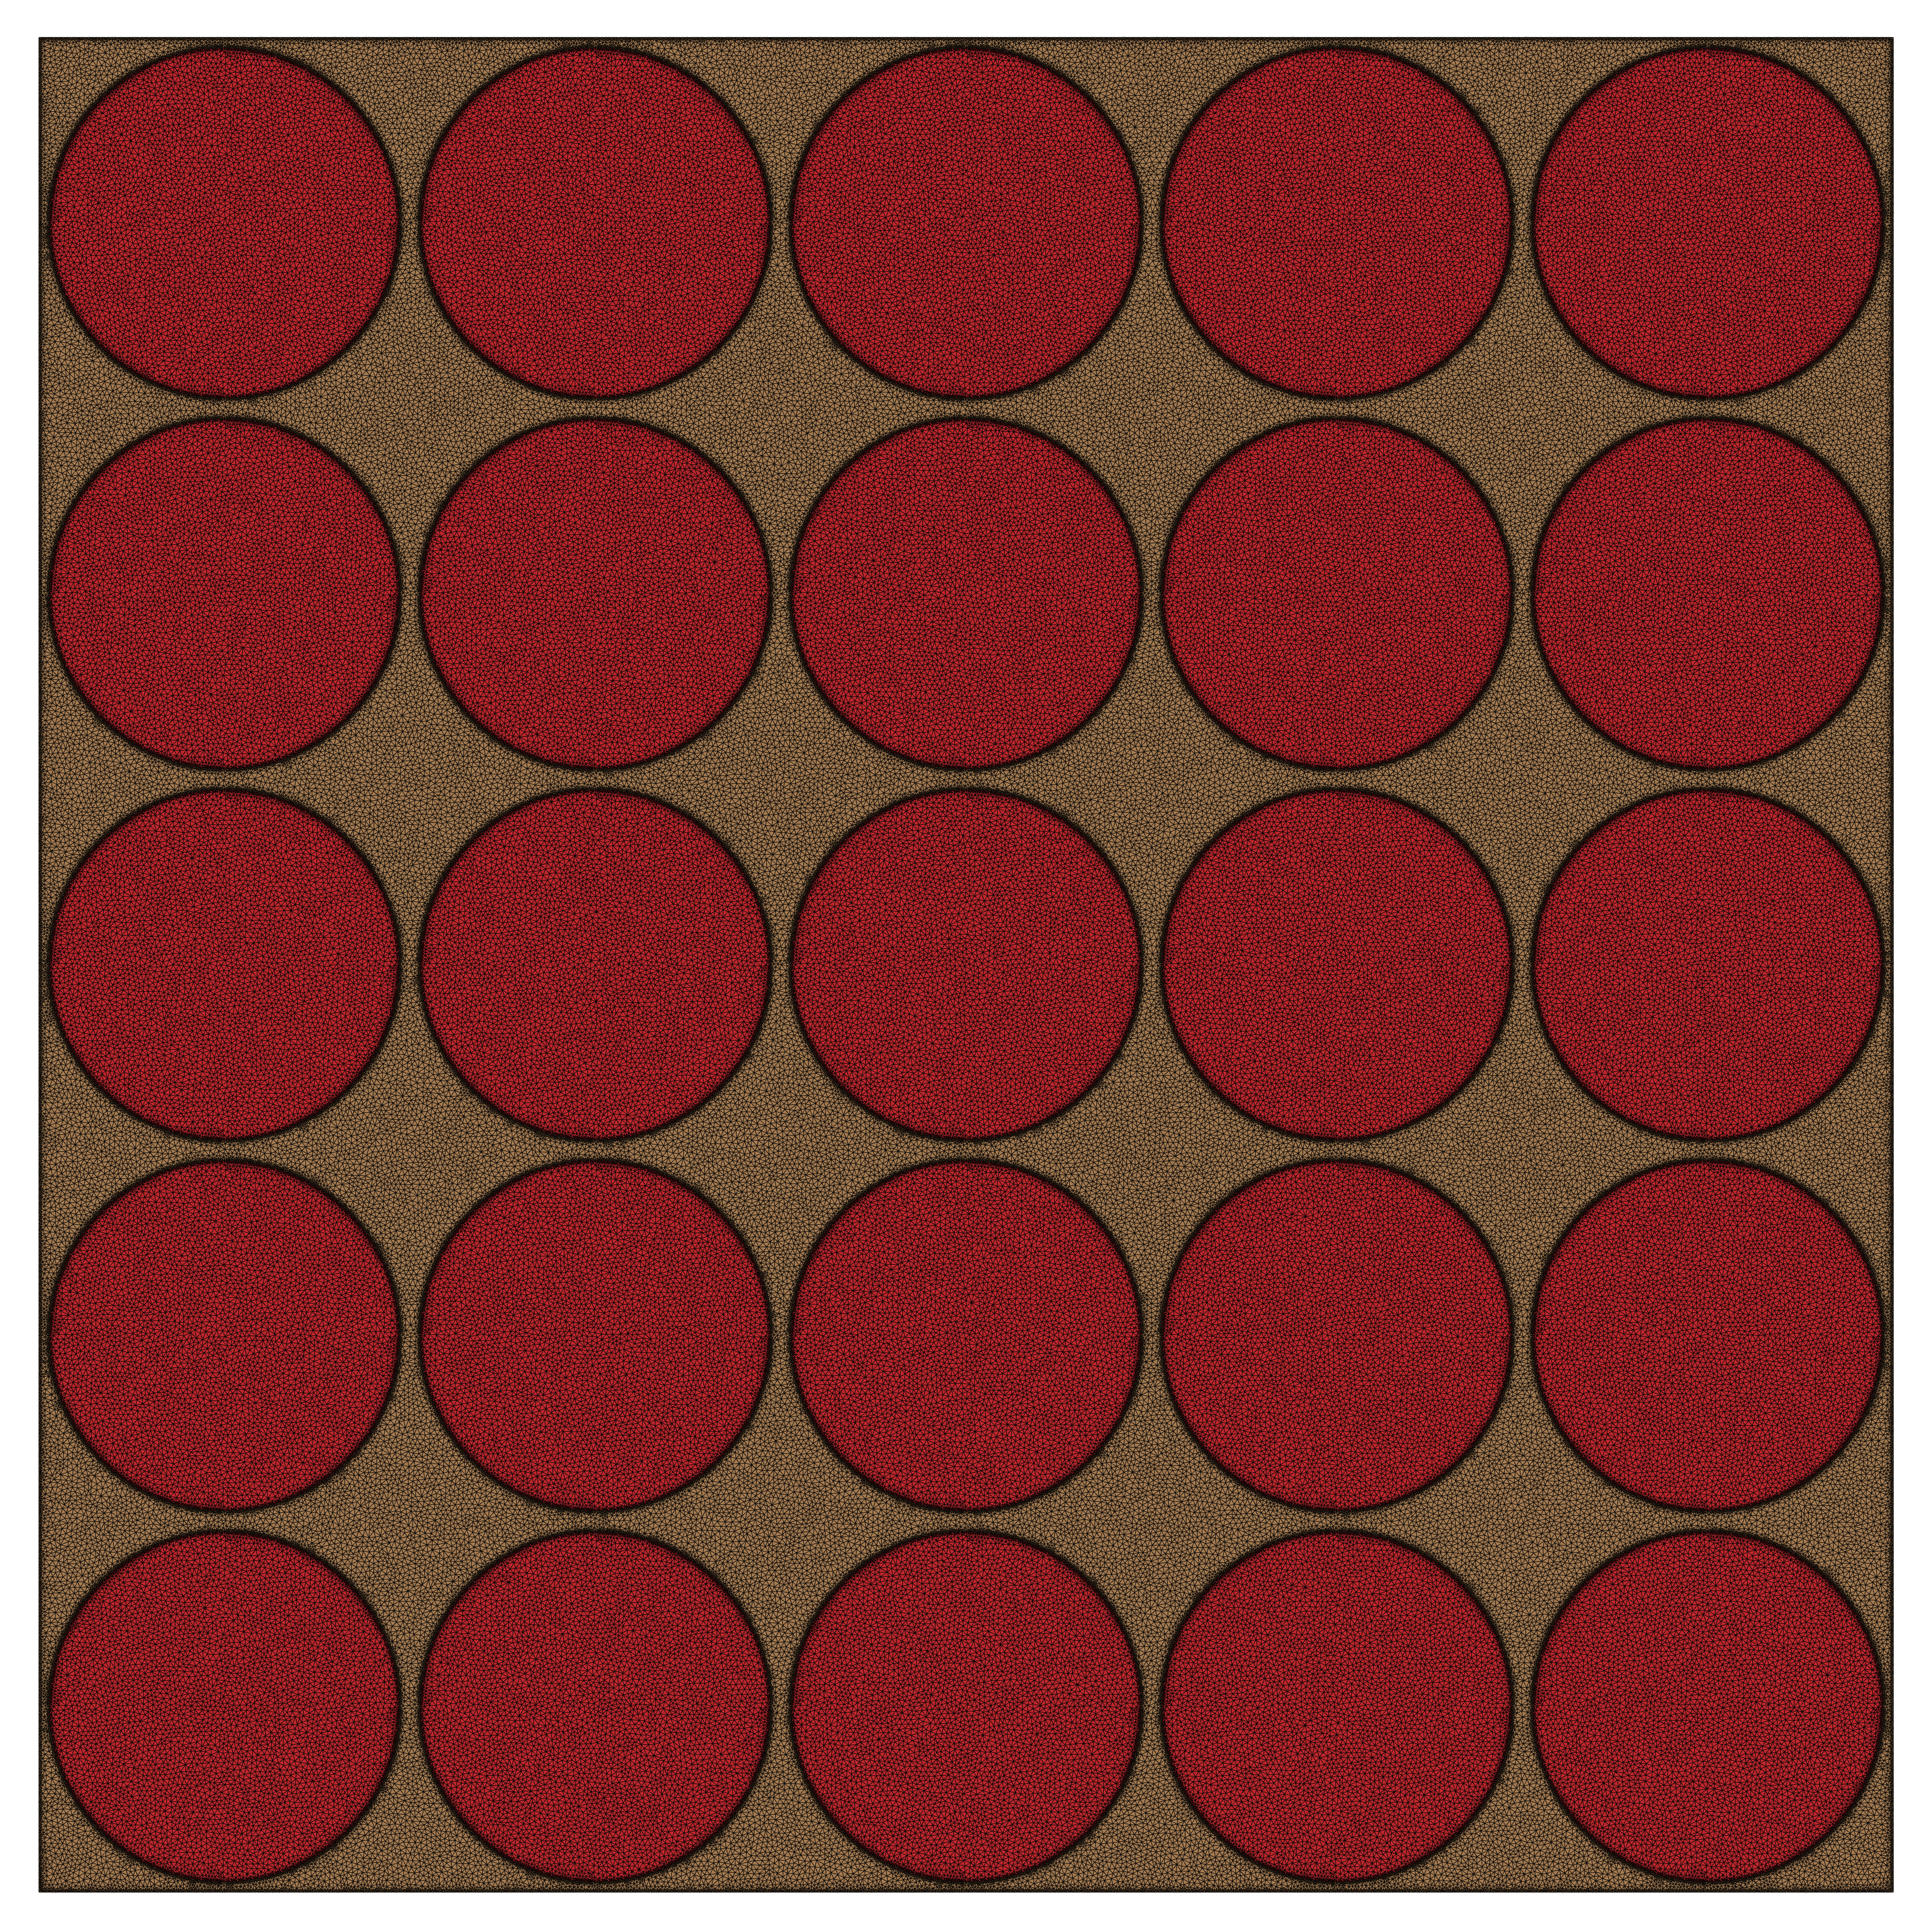
\includegraphics[width=\linewidth]{test_mesh_8.png}
	\caption{Mesh del volume rappresentativo con 756.787 DoF}\label{fig:Mesh}
\end{figure}



\subsection{Codice}

\subsubsection{Condizioni al bordo}

DESCriVI CODICE BORDO

\subsection{Analisi di convergenza}
\label{sec:convergenza}

Per effettuare l'analisi a convergenza è stata implementata una routine che ripete diverse volte l'omogenizzazione citata in \cref{sec:homogen} andando ad infittire la mesh. I risultati sono presenti in Tabella \ref{tab:convergence} e in \cref{fig:convergence}.

Analizzando i risultati è stato preso come valore ottimo quello ottenuto nell'iterazione 8 che presenta un errore rispetto il risultato ideale dello $0.11\%$ a fronte di differenza di impegno computazionale del $83\%$. 



\begin{figure}[bt!] %% preferably at bottom or top of column
	\centering
	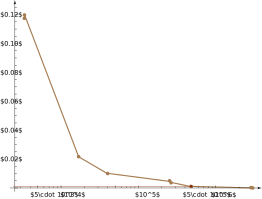
\includegraphics[width=\linewidth]{test_data.pdf}
	\caption{Analisi di convergenza sul parametro $\mathbb C_{11}$}\label{fig:convergence}
\end{figure}

\begin{table}[bt!]
	\caption{Analisi di convergenza}\label{tab:convergence}
	\begin{tabular}{l r r l}
		\toprule
Iterazione&	$C_{11}^{(om)}$ & DoF &  Time (s)\\
		\midrule
	1&		$845.289$ &$3368 $ &  $4.8125 $\\
			2&	$846.427$ & $3384$ &  $4.7500 $\\
			3&	$ 772.214$ &$ 16874$  &  $ 8.5625$\\
			4&$ 763.611$ &$ 39022$  &$ 14.0625$   \\
			5&$ 759.333$ &$ 253262$  & $ 60.7656$     \\
		6&	$ 759.333$ & $ 253316$ & $ 59.2188$     \\
		7&	$758.829 $ &$ 263104$  & $ 61.6563$     \\
		8&	$ 756.787$ &$ 453436$  & $95.2344 $     \\
		9&	$ 755.942$ &$2800338 $  &  $509.141 0$    \\
		10&	$755.903 $ &$ 3024312$  &  $ 555.0630$    \\
		\bottomrule
	\end{tabular}
\end{table}



\section{Disponibilità del codice e materiale aggiuntivo}




\subsection{Lista delle abbreviazioni}

\begin{itemize}
	\item RVE , rappresentative volume element 
	\item $\mathbb C^{(om)}$:,matrice di rigidezza ottenuta dall'omogenizzazione
	\item $\cdot_b$, parametri che fanno riferimento all'osso
	\item $\cdot_m$, parametri che fanno riferimento al midollo
	\item DoF, degrees of freedom
\end{itemize}
 







%% Specify your .bib file name here, without the extension
\bibliography{paper-refs}




\end{document}
